\makeatletter
\def\input@path{{../template/adapter/aljabr-1/edition/}{../template/adapter/aljabr-1/}}
\makeatother
\documentclass[draftmark=false,colors=true,fontsetup=font-setup-open.tex,titlesetup=titles-setup.tex]{AJbook}
\usepackage[unicode,bookmarksnumbered]{hyperref}
\usepackage{ajbook-page-layout,ajbook-cover,enumitem}
\usepackage[
  math-style=ISO,bold-style=ISO,
  mathrm=sym,mathit=sym,mathbf=sym,mathsf=sym,mathtt=sym
]{unicode-math}
\usepackage{arydshln}
% Use the Book face for every mathematical alphabet, including upright operators.
\unimathsetup{mathrm=sym,mathit=sym,mathbf=sym,mathsf=sym,mathtt=sym}
\setmathfont{NewCMMath-Book.otf}
\setoperatorfont{\symup}

% Keep amsopn's literal punctuation in Unicode math's main family as well.
% In particular, its legacy mathcodes otherwise draw the dots of p.v. in CMMI.
\makeatletter
\renewcommand*{\newmcodes@}{%
  \Umathcode"0027=0 \symoperators "0027\relax
  \Umathcode"002A=0 \symoperators "002A\relax
  \Umathcode"002E=0 \symoperators "002E\relax
  \Umathcode"002D=0 \symoperators "002D\relax
  \Umathcode"002F=0 \symoperators "002F\relax
  \Umathcode"003A=0 \symoperators "003A\relax
}
\makeatother

% Keep the existing bold commands on the OpenType mathematical alphabets.
\ExplSyntaxOn
\DeclareRobustCommand{\bm}[1]{%
  \regex_match:nnTF { \A [A-Za-z]+ \Z } {#1}
    { \symbfit{#1} }
    { \symbf{#1} }
}
\ExplSyntaxOff
\DeclareRobustCommand{\boldsymbol}[1]{\bm{#1}}

\numberwithin{equation}{chapter}
\counterwithin{figure}{chapter}
\AtBeginDocument{%
  \theoremstyle{plain}%
  \theoremheaderfont{\sffamily\bfseries\thmheiti}%
  \theorembodyfont{\fangsong}%
  \theoremseparator{\enspace}%
  \theoremsymbol{}%
  \newtheorem{RiemannDefinition}{Definition}[section]%
  \renewcommand{\theRiemannDefinition}{\arabic{section}.\arabic{RiemannDefinition}}%
  \newtheorem{RiemannTheorem}[RiemannDefinition]{Theorem}%
  \newtheorem{RiemannLemma}[RiemannDefinition]{Lemma}%
  \newtheorem{RiemannProposition}[RiemannDefinition]{Proposition}%
  \newtheorem{RiemannCorollary}[RiemannDefinition]{Corollary}%
  \theorembodyfont{\normalfont}%
  \newtheorem{RiemannExample}[RiemannDefinition]{Example}%
  \newtheorem{RiemannRemark}[RiemannDefinition]{Remark}%
  \newtheorem{RiemannExercise}[RiemannDefinition]{Exercise}%
  \theoremstyle{nonumberplain}%
  \theoremheaderfont{\sffamily\bfseries\CJKfamily{pffont}}%
  \theoremsymbol{\openbox}%
  \newtheorem{RiemannProof}{Proof}%
  \setlength{\abovedisplayskip}{8pt}%
  \setlength{\belowdisplayskip}{8pt}%
  \setlength{\abovedisplayshortskip}{8pt}%
  \setlength{\belowdisplayshortskip}{8pt}%
}
\makeatletter
% For stages of the translation where the target is not yet in the manuscript,
% retain a verified link to its page in the original. No provisional aux labels.
\newcommand{\RGRegisterSourceRef}[3]{%
  \expandafter\def\csname RGsourcepage:#1\endcsname{#3}%
  \expandafter\def\csname RGsourcevalue:#1\endcsname{#2}%
}
\newcommand{\RGref}[1]{%
  \@ifundefined{r@#1}{%
    \@ifundefined{RGsourcepage:#1}{\ref{#1}}{%
      \href[page=\csname RGsourcepage:#1\endcsname]{../../input/source/An Introduction to Riemannian Geometry.pdf}{\csname RGsourcevalue:#1\endcsname}%
    }%
  }{\ref{#1}}%
}
\newcommand{\RGbiblabel}[2][]{%
  \phantomsection
  \begingroup\def\@currentlabel{#2}\label{bib:#1#2}\endgroup
}
\newcommand{\RGsolution}[2]{%
  \item[(\ref{#1})]\leavevmode\phantomsection
  \begingroup\edef\@currentlabel{\getrefnumber{#1}}\label{sol:#2}\endgroup
}
\makeatother
\newcommand{\RGcite}[1]{[\RGref{bib:#1}]}
\newcommand{\RGReferenceSection}{%
  \section*{参考文献}%
  \phantomsection
  \addcontentsline{toc}{section}{参考文献}%
}
\newcommand{\RGfigure}[3][.6\textwidth]{%
  \begin{figure}[htbp]
  \centering
  \includegraphics[width=#1]{figures/#2.pdf}
  \caption{#3}\label{fig:#2}
  \end{figure}%
}

% Original cross-references without a verifiable target: see whole-book QA.
\RGRegisterSourceRef{src:unlocated-cartan-formula}{9}{142}
\RGRegisterSourceRef{src:immersion-section-in-chapter-one}{4.5}{166}

\hypersetup{pdftitle={Riemann 几何引论},pdfauthor={Leonor Godinho, José Natário}}
\begin{document}
\renewcommand{\figurename}{Fig.}
\hypersetup{pageanchor=false}
\begingroup
\setCJKfamilyfont{cover-title}[
  Path=../template/adapter/aljabr-1/edition/fonts/noto-serif-cjk-sc/,
  BoldFont=NotoSerifCJKsc-Bold.otf
]{NotoSerifCJKsc-Bold.otf}
\setCJKfamilyfont{cover-secondary}{Noto Sans CJK SC}
\colorlet{CoverSubtitle}{black!62}
\colorlet{octa}{cyan!50!gray}
\providecommand{\identity}{\ensuremath{\mathrm{id}}}
\pgfmathsetseed{20261023}
\begin{titlepage}
\begin{tikzpicture}[remember picture, overlay, pencildraw/.style={
  color=octa, thick, decorate,
  decoration={random steps, segment length=1pt, amplitude=0.7pt}
}]
  % The band and the text column are anchored independently to the page.
  \shade[top color=gray, bottom color=black]
    ([xshift=11mm, yshift=-29mm] current page.north west) rectangle ++(4.4mm,-88mm);
  \node[anchor=north west, inner sep=0pt, outer sep=0pt]
    at ([xshift=24mm, yshift=-33mm] current page.north west) {%
    \begin{minipage}[t]{\dimexpr\paperwidth-48mm\relax}
      \raggedright\CJKfamily{cover-secondary}
      \fontspec[BoldFont=texgyreheros-bold.otf]{texgyreheros-regular.otf}
      \setlength{\parindent}{0pt}%
      \setlength{\parskip}{0pt}%
      {\fontsize{40}{48}\selectfont\bfseries\CJKfamily{cover-title}
        Riemann 几何引论\par}
      \vspace{6pt}
      {\fontsize{18}{24}\selectfont\color{CoverSubtitle}
        在力学与相对论中的应用\par}
      \vspace{20pt}
      {\fontsize{22}{28}\selectfont\bfseries
        An Introduction to Riemannian Geometry\par}
      \vspace{4pt}
      {\fontsize{15}{20}\selectfont\color{CoverSubtitle}
        With Applications to Mechanics and Relativity\par}
      \vspace{13pt}
      {\color{black!55}\rule{\linewidth}{0.8pt}\par}
      \vspace{9pt}
      {\fontsize{16}{22}\selectfont
        \mbox{Leonor Godinho, José Natário}\enspace {\fontsize{13}{18}\selectfont 著}\par}
    \end{minipage}%
  };

  % AJbook cover illustration: Wen-Wei Li (2022), CC BY 4.0.
  \coordinate (pic) at ([xshift=-23em, yshift=22em] current page.south east);
  \coordinate (pic2) at ([xshift=3em] pic);
  \begin{scope}[shift=(pic2), scale=1.5, opacity=0.55]
    \node (P0) at (90:2.3cm) {$((X \otimes Y) \otimes Z) \otimes W$};
    \node (P1) at (90+72:2cm) {$(X \otimes (Y \otimes Z)) \otimes W$};
    \node (P2) at (90+2*72:2cm) {\makebox[5ex][r]{$X \otimes ((Y \otimes Z) \otimes W)$}};
    \node (P3) at (90+3*72:2cm) {\makebox[5ex][l]{$X \otimes (Y \otimes (Z \otimes W))$}};
    \node (P4) at (90+4*72:2cm) {$(X \otimes Y) \otimes (Z \otimes W)$};
    \path[commutative diagrams/.cd, every arrow, every label]
      (P0) edge node[swap] {$a(X,Y,Z) \otimes \identity_W$} (P1)
      (P1) edge node[swap] {$a(X, Y \otimes Z, W)$} (P2)
      (P2) edge node[swap, inner sep=1em] {$\identity_X \otimes a(Y,Z,W)$} (P3)
      (P3) edge node {$a(X,Y,Z \otimes W)$} (P4)
      (P0) edge node {$a(X \otimes Y, Z, W)$} (P4);
  \end{scope}
  \begin{scope}[shift=(pic), rotate=-30, scale=2]
    \coordinate (A1) at (pic);
    \coordinate (A2) at (6em, 2em);
    \coordinate (A3) at (10em, 0);
    \coordinate (A4) at (4em, -2em);
    \coordinate (B1) at (5em, 5em);
    \coordinate (B2) at (5em, -5em);
  \end{scope}
  \begin{scope}[loosely dashed, opacity=0.6]
    \draw[pencildraw] (A1) -- (A2) -- (A3);
    \draw[pencildraw] (B1) -- (A2) -- (B2);
  \end{scope}
  \draw[pencildraw, fill=octa!10, opacity=0.6] (A1) -- (A4) -- (B1);
  \draw[pencildraw, fill=octa!20, opacity=0.6] (A1) -- (A4) -- (B2);
  \draw[pencildraw, fill=octa!30, opacity=0.6] (A3) -- (A4) -- (B1);
  \draw[pencildraw, fill=octa!50, opacity=0.6] (A3) -- (A4) -- (B2);
  \draw[pencildraw] (B1) -- (A1) -- (B2) -- (A3) -- cycle;
\end{tikzpicture}
\cleardoublepage
\end{titlepage}
\endgroup

% Bookmark the heading when AJbook prints the contents, after the page break.
\makeatletter
\let\RGContentsChapterHead\@makeschapterhead
\renewcommand{\@makeschapterhead}[1]{%
  \pdfbookmark[0]{\contentsname}{front:contents}%
  \RGContentsChapterHead{#1}%
}
\frontmatter
\let\@makeschapterhead\RGContentsChapterHead
\makeatother
\clearpage
\hypersetup{pageanchor=true}
\makeatletter
\let\RGPrefaceChapterHead\@makeschapterhead
\renewcommand{\@makeschapterhead}[1]{\phantomsection\RGPrefaceChapterHead{#1}}
\chapter*{序言}
\let\@makeschapterhead\RGPrefaceChapterHead
\makeatother
\addcontentsline{toc}{chapter}{序言}
\markboth{序言}{序言}
\enlargethispage{\baselineskip}

本书以一门自 2002 年起在 Instituto Superior Técnico (里斯本) 面向数学, 物理和工程专业学生讲授的一学期课程为基础. 本书旨在简要介绍微分几何, 包括微分形式, 随后介绍 Riemann 几何的主要思想 (测地线的极小性质, 完备性和曲率). 最后两章给出若干可能的应用; 这两章也曾分别用于一学期的几何力学和广义相对论课程. 我们希望它们能让数学专业的学生体会 Riemann 几何的用处, 也能让物理和工程专业的学生更有动力学习相关数学背景.

我们假定读者具备线性代数, 多元微积分和微分方程的基本知识, 以及拓扑与代数的初步概念. 为方便读者 (尤其是物理和工程专业的学生), 我们在各章末尾按需归纳了这些背景材料中的主要定义和结果.

为了帮助读者检验并巩固自己的理解, 也为了介绍正文未涉及的重要思想和例子, 我们编入了 330 多道习题, 其中约 140 道在第~\RGref{chap:solutions}~章中给出解答 (全套习题的解答可提供给任课教师). 我们希望本书由此适合自学, 同时仍保留足够多没有给出解答的习题, 供读者挑战.

下面简要介绍各章的内容.

第~\RGref{chap:differentiable-manifolds}~章讨论微分几何的基本概念: 可微流形与可微映射, 向量场和 Lie 括号. 此外, 我们简要介绍 Lie 群和 Lie 群作用.

第~\RGref{chap:differential-forms}~章专门讨论微分形式, 涵盖楔积, 拉回, 外微分, 积分和 Stokes 定理等标准内容.

第~\RGref{chap:riemannian-manifolds}~章引入 Riemann 流形, 讨论 Levi–Civita 联络, 测地线的极小性质和 Hopf–Rinow 定理.

第~\RGref{chap:curvature}~章讨论曲率的概念. 特别地, 我们利用 Cartan 结构方程所提供的有力计算方法证明 Gauss–Bonnet 定理. 我们也讨论常曲率和等距嵌入.

第~\RGref{chap:geometric-mechanics}~章概述几何力学, 包括完整和非完整系统, Lagrange 力学与 Hamilton 力学, 完全可积系统和约化.

第~\RGref{chap:relativity}~章讨论广义相对论, 首先从几何角度介绍狭义相对论. 我们通过 Newton 引力的 Cartan 联络表述引出 Einstein 方程, 并研究 Schwarzschild 解 (包括黑洞) 和宇宙学等基本例子. 最后, 我们讨论因果性以及著名的 Hawking 和 Penrose 奇性定理. 这些定理在入门教材中并不常见, 却是 Riemann 几何很有趣的应用.

最后, 我们感谢许多曾阅读本书全部或部分内容的同事和学生, 感谢他们提出的宝贵意见与建议. 特别感谢我们的同事和朋友 Pedro Girão.

\mainmatter
\chapter{可微流形}\label{chap:differentiable-manifolds}
\begingroup
\renewcommand{\thefootnote}{}
\footnotetext{\textcopyright\ Springer International Publishing Switzerland 2014.
  L. Godinho and J. Natário, \emph{An Introduction to Riemannian Geometry},
  Universitext. DOI \href{https://doi.org/10.1007/978-3-319-08666-8_1}{10.1007/978-3-319-08666-8\_1}.}
\endgroup

在纯粹数学和应用数学中, 我们经常遇到局部看起来像 $\mathbb{R}^n$ 的空间, 意思是这些空间在局部可以用 $n$ 个坐标来参数化. 例如, $n$ 维球面 $S^n\subset\mathbb{R}^{n+1}$, 或刚体的构型集合 $\mathbb{R}^3\times SO(3)$. 我们或许会预期微积分的基本工具在这些空间上仍然适用. 然而, 由于一般没有典范的局部坐标选取, 在讨论导数或积分等概念时必须格外小心: 这些概念在 $\mathbb{R}^n$ 中的定义依赖于优先选取的 Cartesian 坐标.

本章的主题是这类空间 (称为\textbf{可微流形}) 的严格定义, 以及与之有关的微分概念. 尽管直观想法看来相当简单, 而且事实上可以追溯到 Gauss 和 Riemann, 但直到 1936 年才由 Whitney 给出形式定义.

局部看起来像 $\mathbb{R}^n$ 的空间, 通过\textbf{拓扑流形}的定义加以形式化: 拓扑流形是局部同胚于 $\mathbb{R}^n$ 的拓扑空间. 我们将在第~\RGref{sec:topological-manifolds}~节研究它们, 并讨论若干例子, 尤其是 2 维的例子 (曲面).

第~\RGref{sec:differentiable-manifolds}~节把可微流形定义为坐标变换 (从 $\mathbb{R}^n$ 到 $\mathbb{R}^n$ 的映射) 光滑 ($C^\infty$) 的拓扑流形. 由此可以把\textbf{可微函数}定义为局部坐标表达式光滑的函数 (第~\RGref{sec:differentiable-maps}~节), 把\textbf{切向量}定义为作用于实值可微函数的方向导数算子 (第~\RGref{sec:tangent-space}~节). 第~\RGref{sec:immersions-embeddings}~节考察可微映射的两个重要例子, 即\textbf{浸入}和\textbf{嵌入}.

\textbf{向量场}及其\textbf{流}是第~\RGref{sec:vector-fields}~节的主要内容. 我们定义向量场之间的一种自然微分运算, 称为 \textbf{Lie 括号}; 它度量这些向量场的流的不交换性, 在微分几何中起着核心作用.

第~\RGref{sec:lie-groups}~节讨论一类重要的可微流形, 它们同时也是群, 称为 \textbf{Lie 群}. 我们将说明, 每个 Lie 群都可对应一个 \textbf{Lie 代数}, 即一个带有 Lie 括号的向量空间. 本节也讨论在 Lie 群作用下得到的流形的\textbf{商}.

流形的\textbf{可定向性} (与曲面"有两面"这一直观概念密切相关) 和\textbf{带边界流形} (推广有闭曲线作为边界的曲面, 或有闭曲面作为边界的立体这一概念), 分别在第~\RGref{sec:orientability}~节和第~\RGref{sec:manifolds-with-boundary}~节研究. 陈述著名的 Stokes 定理需要这两个概念, 该定理将在第~\RGref{chap:differential-forms}~章证明.

\section{拓扑流形}\label{sec:topological-manifolds}

本节先研究局部形似 $\mathbb{R}^n$ 的空间, 即每个点都有一个与 $\mathbb{R}^n$ 的某个开子集同胚的邻域.

\begin{RiemannDefinition}\label{def:topological-manifold}
$n$ 维\textbf{拓扑流形} $M$ 是满足以下性质的拓扑空间:
\begin{enumerate}[label=(\roman*),leftmargin=*]
\item $M$ 是 \textbf{Hausdorff} 的, 即对 $M$ 中任意两个不同的点 $p_1,p_2$, 分别存在它们的邻域 $V_1,V_2$, 使得 $V_1\cap V_2=\varnothing$.
\item 每个点 $p\in M$ 都有一个与 $\mathbb{R}^n$ 的某个开子集 $U$ 同胚的邻域 $V$.
\item $M$ 满足\textbf{第二可数公理}, 即 $M$ 的拓扑具有可数基.
\end{enumerate}
\end{RiemannDefinition}

在定义中加入条件 (i) 和 (iii), 是为了避免这些空间的拓扑过于奇特. 特别地, Hausdorff 公理保证收敛序列的极限唯一. 这一公理与第二可数公理一起保证了单位分解的存在性 (参见第~\RGref{chap:differential-forms}~章第~\RGref{subsec:notes-integration-on-manifolds}~节). 我们将看到, 单位分解是微分几何的一项基本工具.

\begin{RiemannRemark}\label{rem:topological-manifolds-low-dimension}
若 $M$ 的维数为零, 则 $M$ 是一个赋有离散拓扑的可数集 ($M$ 的每个子集都是开集). 若 $\dim M=1$, 则 $M$ 局部同胚于开区间; 若 $\dim M=2$, 则 $M$ 局部同胚于开圆盘, 依此类推.
\end{RiemannRemark}

\begin{RiemannExample}\label{ex:manifolds-from-euclidean-space}
\begin{enumerate}[label=(\arabic*),leftmargin=*]
\item $\mathbb{R}^n$ 的每个开子集 $M$ 赋予子空间拓扑 (即 $U\subset M$ 是开集, 当且仅当 $U=M\cap V$, 其中 $V$ 是 $\mathbb{R}^n$ 的开集) 后, 都是拓扑流形.
\item (\emph{圆}) 赋有子空间拓扑的\textbf{圆}
\[
  S^1=\{(x,y)\in\mathbb{R}^2\mid x^2+y^2=1\}
\]
是 1 维拓扑流形. 条件 (i) 和 (iii) 继承自周围空间. 另外, 对每个点 $p\in S^1$, 至少有一条坐标轴不平行于 $S^1$ 在 $p$ 处的法向量 $n_p$. 投影到这条坐标轴, 就得到 $p$ 的一个 (足够小的) 邻域 $V$ 与 $\mathbb{R}$ 中一个区间之间的同胚.
\RGfigure[.46\textwidth]{circle-sphere-torus}{\textbf{a} $S^1$; \textbf{b} $S^2$; \textbf{c} 旋转环面}
\item (\emph{2 维球面}) 容易推广上一个例子, 以说明带有子空间拓扑的 \textbf{2 维球面}
\[
  S^2=\{(x,y,z)\in\mathbb{R}^3\mid x^2+y^2+z^2=1\}
\]
是 2 维拓扑流形.
\item (\emph{旋转环面}) 与前面的例子一样, 可以说明把一个圆绕一条与它不相交的轴旋转所得的旋转曲面是 2 维拓扑流形 (Fig.~\ref{fig:circle-sphere-torus}).
\item 立方体的表面是拓扑流形 (同胚于 $S^2$).
\end{enumerate}
\end{RiemannExample}

\begin{RiemannExample}\label{ex:manifolds-by-identifying-edges}
也可以用同胚把某些多边形的边等同起来, 从而得到拓扑流形. 例如, 正方形的边可以按几种不同的方式等同 (见 Fig.~\ref{fig:edge-identifications-torus-klein} 和 Fig.~\ref{fig:edge-identifications-projective-plane}):
\begin{enumerate}[label=(\arabic*),leftmargin=*]
\item (\emph{环面}) \textbf{环面} $T^2$ 是单位正方形 $Q=[0,1]^2\subset\mathbb{R}^2$ 对等价关系
\[
  (x,y)\sim(x+1,y)\sim(x,y+1),
\]
所取的商, 赋以商拓扑 (参见第~\RGref{subsec:notes-topological-manifolds}~节).
\item (\emph{Klein 瓶}) \textbf{Klein 瓶} $K^2$ 是 $Q$ 对等价关系
\[
  (x,y)\sim(x+1,y)\sim(1-x,y+1)
\]
所取的商.
\RGfigure[.52\textwidth]{edge-identifications-torus-klein}{\textbf{a} 环面 ($T^2$); \textbf{b} Klein 瓶 ($K^2$)}
\RGfigure[.52\textwidth]{edge-identifications-projective-plane}{射影平面 ($\mathbb{R}P^2$)}
\item (\emph{射影平面}) \textbf{射影平面} $\mathbb{R}P^2$ 是 $Q$ 对等价关系
\[
  (x,y)\sim(x+1,1-y)\sim(1-x,y+1)
\]
所取的商.
\end{enumerate}
\end{RiemannExample}

\begin{RiemannRemark}\label{rem:connected-sums-of-surfaces}
\begin{enumerate}[label=(\arabic*),leftmargin=*]
\item 唯一的紧致连通 1 维拓扑流形是圆 $S^1$ (见 \RGcite{Mil97}).
\item 两个拓扑流形 $M$ 和 $N$ 的\textbf{连通和}是如下得到的拓扑流形 $M\#N$: 从每个流形中去掉一个同胚于球的开集, 再用一个同胚将边界 (它们必须与球面同胚) 粘合起来 (参见 Fig.~\ref{fig:connected-sum-of-tori}). 可以证明, 任何紧致连通 2 维拓扑流形要么同胚于 $S^2$, 要么同胚于 Example~\ref{ex:manifolds-by-identifying-edges} 中的流形的连通和 (见 [\RGref{bib:Blo96}, \RGref{bib:Mun00}]).
\end{enumerate}
\end{RiemannRemark}

\RGfigure[.69\textwidth]{connected-sum-of-tori}{两个环面的连通和}
\RGfigure[.46\textwidth]{cylinder-and-mobius-band}{\textbf{a} 圆柱面; \textbf{b} Möbius 带}

若不把正方形所有的边都等同起来, 我们会得到圆柱面或 \textbf{Möbius 带} (参见 Fig.~\ref{fig:cylinder-and-mobius-band}). 这些拓扑空间是\textbf{带边界流形}的例子.

\begin{RiemannDefinition}\label{def:topological-manifold-with-boundary}
考虑\textbf{闭半空间}
\[
  \mathbb{H}^n=\{(x^1,\ldots,x^n)\in\mathbb{R}^n\mid x^n\geq 0\}.
\]
\textbf{带边界的拓扑流形}是一个具有可数开集基的 Hausdorff 空间 $M$, 使得每个点 $p\in M$ 都有一个邻域 $V$, 它或者与 $\mathbb{H}^n\setminus\partial\mathbb{H}^n$ 的某个开子集 $U$ 同胚, 或者与 $\mathbb{H}^n$ 的某个开子集 $U$ 同胚且 $p$ 对应于 $\partial\mathbb{H}^n$ 中的一个点. 第一类点称为\textbf{内点}, 其余的称为\textbf{边界点}.
\end{RiemannDefinition}

\RGfigure[.55\textwidth]{mobius-band-in-two-surfaces}{Möbius 带位于 \textbf{a} Klein 瓶内; \textbf{b} 实射影平面内}
\RGfigure[.73\textwidth]{disk-in-projective-plane}{实射影平面内的圆盘}

边界点的集合 $\partial M$ 称为 $M$ 的\textbf{边界}, 它是一个 $(n-1)$ 维流形.

\begin{RiemannRemark}\label{rem:mobius-band-decompositions}
\begin{enumerate}[label=\arabic*.,leftmargin=*]
\item 制作一个 Möbius 带的纸模型, 就容易验证其边界同胚于一个圆 (不是两个不相交的圆), 并且它只有一面 (参见 Fig.~\ref{fig:cylinder-and-mobius-band}).
\item Klein 瓶和实射影平面都含有 Möbius 带 (参见 Fig.~\ref{fig:mobius-band-in-two-surfaces}). 在射影平面上去掉这条带, 就得到一个圆盘 (参见 Fig.~\ref{fig:disk-in-projective-plane}). 换言之, 把一个 Möbius 带和一个圆盘沿各自的边界粘合, 就可以得到 $\mathbb{R}P^2$.
\end{enumerate}
\end{RiemannRemark}

若两个拓扑流形同胚, 我们就把它们视为相同. 例如, $\mathbb{R}^3$ 中半径不同的球面彼此同胚, Fig.~\ref{fig:knotted-and-unknotted-tori} 中的两个曲面也同胚. 实际上, 可以沿一个圆切开环面, 将它打结后再粘起来, 得到打结的环面. 一个显然的同胚便是将原环面上的每个点送到切开和粘合后的最终位置的映射 (不过, 这个同胚不能延拓为周围空间 $\mathbb{R}^3$ 的一个同胚).

\RGfigure[.49\textwidth]{knotted-and-unknotted-tori}{两个同胚的拓扑流形}

\begin{RiemannExercise}\label{ex:topological-manifolds}
\begin{enumerate}[label=(\arabic*),ref=\arabic*,leftmargin=*]
\item\label{ex:recognize-topological-manifolds} 下列哪些集合 (带有子空间拓扑) 是拓扑流形?
\begin{enumerate}[label=(\alph*),leftmargin=*]
\item $D^2=\{(x,y)\in\mathbb{R}^2\mid x^2+y^2<1\}$;
\item $S^2\setminus\{p\}$ ($p\in S^2$);
\item $S^2\setminus\{p,q\}$ ($p,q\in S^2$, $p\ne q$);
\item $\{(x,y,z)\in\mathbb{R}^3\mid x^2+y^2=1\}$;
\item $\{(x,y,z)\in\mathbb{R}^3\mid x^2+y^2=z^2\}$;
\end{enumerate}
\item\label{ex:classify-topological-manifolds} 上述哪些流形同胚?
\item\label{ex:klein-bottle-from-mobius-bands} 证明可以通过一个边界同胚将两个 Möbius 带粘合在一起, 从而得到 Klein 瓶 $K^2$.
\item\label{ex:connected-sum-identities} 证明:
\begin{enumerate}[label=(\alph*),leftmargin=*]
\item 对任意 2 维拓扑流形 $M$, $M\#S^2=M$;
\item $\mathbb{R}P^2\#\mathbb{R}P^2=K^2$;
\item $\mathbb{R}P^2\#T^2=\mathbb{R}P^2\#K^2$.
\end{enumerate}
\item\label{ex:euler-characteristic-of-surfaces} 2 维拓扑流形 $M$ 的一个\textbf{三角剖分}, 是将 $M$ 分解为有限个三角形 (即与 $\mathbb{R}^2$ 中三角形同胚的子集), 使任意两个三角形的交集或者是一条公共边, 或者是一个公共顶点, 或者为空 (可以证明这样的三角剖分总是存在). $M$ 的 \textbf{Euler 特征数}为
\[
  \chi(M):=V-E+F,
\]
其中 $V,E,F$ 分别为给定三角剖分的顶点数, 边数和面数 (可以证明它是良定义的, 即不依赖于三角剖分的选择). 证明:
\begin{enumerate}[label=(\alph*),leftmargin=*]
\item 给三角剖分增加一个顶点不会改变 $\chi(M)$;
\item $\chi\bigl(S^2\bigr)=2$;
\item $\chi\bigl(T^2\bigr)=0$;
\item $\chi\bigl(K^2\bigr)=0$;
\item $\chi\bigl(\mathbb{R}P^2\bigr)=1$;
\item $\chi(M\#N)=\chi(M)+\chi(N)-2$.
\end{enumerate}
\end{enumerate}
\end{RiemannExercise}

\section{可微流形}\label{sec:differentiable-manifolds}

回顾一下, $n$ 维拓扑流形是具有可数开集基的 Hausdorff 空间, 其中每个点都有一个与 $\mathbb{R}^n$ 的某个开子集同胚的邻域. 设 $U$ 是 $\mathbb{R}^n$ 的一个开子集, $\varphi:U\to\varphi(U)\subset M$ 是从 $U$ 到 $M$ 的一个开子集的同胚, 则每个这样的二元组 $(U,\varphi)$ 都称为一个\textbf{参数化}. 其逆映射 $\varphi^{-1}$ 称为\textbf{坐标系}或\textbf{坐标图}, 集合 $\varphi(U)\subset M$ 称为\textbf{坐标邻域}. 当两个坐标邻域相交时, 我们可以写出相应的坐标变换 (参见 Fig.~\ref{fig:chart-transition-maps}). 得到可微流形的想法是选取一部分参数化, 使得坐标变换都是可微映射.

\RGfigure[.57\textwidth]{chart-transition-maps}{参数化与重叠映射}

\begin{RiemannDefinition}\label{def:differentiable-manifold}
$n$ 维\textbf{可微流形}或\textbf{光滑流形}由一个 $n$ 维拓扑流形 $M$ 和一族定义在开集 $U_\alpha\subset\mathbb{R}^n$ 上的参数化 $\varphi_\alpha:U_\alpha\to M$ 组成, 且满足:
\begin{enumerate}[label=(\roman*),leftmargin=*]
\item 坐标邻域覆盖 $M$, 即 $\bigcup_\alpha\varphi_\alpha(U_\alpha)=M$;
\item 对每一对满足
\[
  W:=\varphi_\alpha(U_\alpha)\cap\varphi_\beta(U_\beta)\ne\varnothing,
\]
的指标 $\alpha,\beta$, 重叠映射
\begin{gather*}
  \varphi_\beta^{-1}\circ\varphi_\alpha:\varphi_\alpha^{-1}(W)\to\varphi_\beta^{-1}(W)\\
  \varphi_\alpha^{-1}\circ\varphi_\beta:\varphi_\beta^{-1}(W)\to\varphi_\alpha^{-1}(W)
\end{gather*}
都是 $C^\infty$ 的;
\item 族 $\mathcal{A}=\{(U_\alpha,\varphi_\alpha)\}$ 关于 (i) 和 (ii) 是极大的, 即如果 $\varphi_0:U_0\to M$ 是一个参数化, 使得对 $\mathcal{A}$ 中的所有 $\varphi$, $\varphi_0^{-1}\circ\varphi$ 和 $\varphi^{-1}\circ\varphi_0$ 都是 $C^\infty$ 的, 那么 $(U_0,\varphi_0)$ 属于 $\mathcal{A}$.
\end{enumerate}
\end{RiemannDefinition}

\begin{RiemannRemark}\label{rem:maximal-and-equivalent-atlases}
\begin{enumerate}[label=(\arabic*),leftmargin=*]
\item 任何满足 (i) 和 (ii) 的族 $\mathcal{A}=\{(U_\alpha,\varphi_\alpha)\}$ 都称为 $M$ 的一个 \textbf{$C^\infty$ 图册}. 如果 $\mathcal{A}$ 还满足 (iii), 就称其为\textbf{极大图册}或\textbf{可微结构}.
\item 条件 (iii) 纯粹是技术性的. 给定 $M$ 上任意图册 $\mathcal{A}=\{(U_\alpha,\varphi_\alpha)\}$, 存在唯一的包含它的极大图册 $\widetilde{\mathcal{A}}$. 实际上, 可以取 $\widetilde{\mathcal{A}}$ 为与 $\mathcal{A}$ 中每个参数化都满足 (ii) 的所有参数化所成的集合. 显然 $\mathcal{A}\subset\widetilde{\mathcal{A}}$, 且容易检验 $\widetilde{\mathcal{A}}$ 满足 (i) 和 (ii). 由构造可知, $\widetilde{\mathcal{A}}$ 关于 (i) 和 (ii) 是极大的. 如果两个图册定义了\phantomsection\label{idx:equivalent-atlases}同一个可微结构, 就称它们\textbf{等价}.
\item 我们也可以通过要求坐标变换是 $C^k$ 映射来定义 $C^k$ 流形 (此时 $C^0$ 流形就表示拓扑流形).
\end{enumerate}
\end{RiemannRemark}

\begin{RiemannExample}\label{ex:examples-of-differentiable-structures}
\begin{enumerate}[label=(\arabic*),ref=\arabic*,leftmargin=*]
\item\label{ex:standard-atlas-on-euclidean-space} 赋有 Euclidean 度量所定义的通常拓扑的空间 $\mathbb{R}^n$ 是 Hausdorff 空间, 并且具有可数的开集基. 例如, 若只考虑一个参数化 $(\mathbb{R}^n,id)$, 则 Definition~\ref{def:differentiable-manifold} 的 (i) 和 (ii) 自然满足, 从而得到 $\mathbb{R}^n$ 的一个图册. 包含这个参数化的极大图册通常称为 $\mathbb{R}^n$ 上的\textbf{标准可微结构}. 当然也可以考虑其他图册. 例如, 取由参数化 $(\mathbb{R}^n,\varphi)$ 定义的图册, 其中 $\varphi(x)=Ax$, $A$ 是非奇异的 $(n\times n)$ 矩阵. 证明这两个图册等价是一道简单的练习.
\item\label{ex:inequivalent-atlases-on-the-line} 一个流形可能有不等价的图册. 考虑 $\mathbb{R}$ 上的两个图册 $\{(\mathbb{R},\varphi_1)\}$ 和 $\{(\mathbb{R},\varphi_2)\}$, 其中 $\varphi_1(x)=x$, $\varphi_2(x)=x^3$. 由于映射 $\varphi_2^{-1}\circ\varphi_1$ 在原点不可微, 这两个图册定义了不同的可微结构 (不过, 我们将看到, 它们彼此微分同胚) [参见 Exercise~\ref{ex:exercise-differentiable-structures}(\ref{ex:prove-inequivalence-of-line-atlases}) 和 Exercise~\ref{ex:properties-of-differentiable-maps}(\ref{ex:properties-of-differentiable-maps-part-six})].
\item\label{ex:open-subsets-inherit-atlases} 光滑流形的每个开子集 $V$ 都是同维数的流形. 实际上, 由于 $V$ 是 $M$ 的子集, 它的子空间拓扑是 Hausdorff 的, 且具有可数的开集基. 此外, 若 $\mathcal{A}=\{(U_\alpha,\varphi_\alpha)\}$ 是 $M$ 的图册, 取所有满足 $\varphi_\alpha(U_\alpha)\cap V\ne\varnothing$ 的 $U_\alpha$, 容易检验参数化族 $\widetilde{\mathcal{A}}=\{(\widetilde U_\alpha,\varphi_\alpha|_{\widetilde U_\alpha})\}$ 是 $V$ 的一个图册, 其中 $\widetilde U_\alpha=\varphi_\alpha^{-1}(V)$.
\item\label{ex:matrix-space-and-general-linear-group} 设 $M_{n\times n}$ 是实系数 $n\times n$ 矩阵的集合. 把矩阵元素排成一行, 可见这个空间就是 $\mathbb{R}^{n^2}$, 因而它是流形. 由第~\ref{ex:open-subsets-inherit-atlases}~个例子可知, $GL(n)=\{A\in M_{n\times n}\mid\det A\ne 0\}$ 也是一个 $n^2$ 维流形. 实际上, 行列式是从 $M_{n\times n}$ 到 $\mathbb{R}$ 的连续映射, 而 $GL(n)$ 是开集 $\mathbb{R}\setminus\{0\}$ 的原像.
\item\label{ex:sphere-atlas-by-coordinate-projections} 考虑 \textbf{$n$ 维球面}
\[
  S^n=\{(x^1,\ldots,x^{n+1})\in\mathbb{R}^{n+1}\mid(x^1)^2+\cdots+(x^{n+1})^2=1\}
\]
以及映射
\[
  \begin{aligned}
  \varphi_i^+&:U\subset\mathbb{R}^n\to S^n\\
  (x^1,\ldots,x^n)&\mapsto(x^1,\ldots,x^{i-1},g(x^1,\ldots,x^n),x^i,\ldots,x^n),
  \end{aligned}
\]
\[
  \begin{aligned}
  \varphi_i^-&:U\subset\mathbb{R}^n\to S^n\\
  (x^1,\ldots,x^n)&\mapsto(x^1,\ldots,x^{i-1},-g(x^1,\ldots,x^n),x^i,\ldots,x^n),
  \end{aligned}
\]
其中
\[
  U=\{(x^1,\ldots,x^n)\in\mathbb{R}^n\mid (x^1)^2+\cdots+(x^n)^2<1\}
\]
且
\[
  g(x^1,\ldots,x^n)=\bigl(1-(x^1)^2-\cdots-(x^n)^2\bigr)^{\frac12}.
\]
球面是 $\mathbb{R}^{n+1}$ 的子集, 因而 (赋予子空间拓扑后) 是 Hausdorff 空间, 且具有可数的开集基. 也容易检验族 $\{(U,\varphi_i^+),(U,\varphi_i^-)\}_{i=1}^{n+1}$ 是 $S^n$ 的图册, 因而这个空间是 $n$ 维流形 (相应的坐标图恰是到超平面 $x^i=0$ 的投影).
\item 可以为立方体的表面 $Q\subset\mathbb{R}^3$ 定义一个图册, 使它成为光滑流形. 假定立方体以原点为中心, 考虑由 $f(x)=x/\lVert x\rVert$ 定义的映射 $f:Q\to S^2$. 于是, 对 $S^2$ 的图册 $\{(U_\alpha,\varphi_\alpha)\}$, 族 $\{(U_\alpha,f^{-1}\circ\varphi_\alpha)\}$ 定义了 $Q$ 的一个图册.
\end{enumerate}
\end{RiemannExample}

\begin{RiemannRemark}\label{rem:topological-manifolds-without-smooth-structure}
有些拓扑流形完全不容许任何可微结构. 实际上, Kervaire 在 1960 年给出了第一个例子 (一个 10 维流形) \RGcite{Ker60}, 不久 Smale 又构造了另一个例子 (维数为 12) \RGcite{Sma60}. 早在 1956 年, Milnor \RGcite{Mil07} 就给出了一个他认为不容许可微结构的 8 维流形的例子, 但这一点直到 1965 年才得到证明 (见 \RGcite{Nov65}).
\end{RiemannRemark}

\begin{RiemannExercise}\label{ex:exercise-differentiable-structures}
\begin{enumerate}[label=(\arabic*),ref=\arabic*,leftmargin=*]
\item\label{ex:compare-atlases-by-union} 证明光滑流形的两个图册 $\mathcal{A}_1$ 和 $\mathcal{A}_2$ 等价, 当且仅当 $\mathcal{A}_1\cup\mathcal{A}_2$ 是图册.
\item\label{ex:open-sets-in-parameterizations} 设 $M$ 是可微流形. 证明集合 $V\subset M$ 是开集, 当且仅当对于一个 $C^\infty$ 图册中的每个参数化 $(U_\alpha,\varphi_\alpha)$, $\varphi_\alpha^{-1}(V)$ 都是 $\mathbb{R}^n$ 的开子集.
\item\label{ex:euclidean-atlases-equivalent} 证明 Example~\ref{ex:examples-of-differentiable-structures}(\ref{ex:standard-atlas-on-euclidean-space}) 中 $\mathbb{R}^n$ 上的两个图册等价.
\item\label{ex:prove-inequivalence-of-line-atlases} 考虑 Example~\ref{ex:examples-of-differentiable-structures}(\ref{ex:inequivalent-atlases-on-the-line}) 中 $\mathbb{R}$ 上的两个图册 $\{(\mathbb{R},\varphi_1)\}$ 和 $\{(\mathbb{R},\varphi_2)\}$, 其中 $\varphi_1(x)=x$, $\varphi_2(x)=x^3$. 证明 $\varphi_2^{-1}\circ\varphi_1$ 在原点不可微, 并由此得出这两个图册不等价.
\item\label{ex:surfaces-as-local-graphs} 回顾初等向量微积分中的定义: 曲面 $S\subset\mathbb{R}^3$ 是一个集合, 对每个 $p\in S$, 在 $\mathbb{R}^3$ 中存在 $p$ 的一个邻域 $V_p$, 并存在一个 $C^\infty$ 映射 $f_p:U_p\to\mathbb{R}$ (其中 $U_p$ 是 $\mathbb{R}^2$ 的开子集), 使得 $S\cap V_p$ 是 $z=f_p(x,y)$, $x=f_p(y,z)$ 或 $y=f_p(x,z)$ 的图像. 证明 $S$ 是 2 维光滑流形.
\item\label{ex:product-differentiable-manifold} (乘积流形) 设 $\{(U_\alpha,\varphi_\alpha)\}$ 和 $\{(V_\beta,\psi_\beta)\}$ 分别为两个光滑流形 $M$ 和 $N$ 的图册. 证明族 $\{(U_\alpha\times V_\beta,\varphi_\alpha\times\psi_\beta)\}$ 是乘积 $M\times N$ 的一个图册. 赋予由这个图册生成的可微结构后, $M\times N$ 称为 $M$ 和 $N$ 的\textbf{乘积流形}.
\item\label{ex:stereographic-sphere-atlas} (球极投影) 考虑带子空间拓扑的 $n$ 维球面 $S^n$, 设 $N=(0,\ldots,0,1)$ 和 $S=(0,\ldots,0,-1)$ 分别为北极和南极. 从 $N$ 出发的\textbf{球极投影}是映射 $\pi_N:S^n\setminus\{N\}\to\mathbb{R}^n$, 它把点 $p\in S^n\setminus\{N\}$ 送到经过 $N$ 和 $p$ 的直线与超平面 $x^{n+1}=0$ 的交点 (参见 Fig.~\ref{fig:stereographic-projection}). 类似地, 从 $S$ 出发的球极投影是映射 $\pi_S:S^n\setminus\{S\}\to\mathbb{R}^n$, 它把 $S^n\setminus\{S\}$ 上的点 $p$ 送到经过 $S$ 和 $p$ 的直线与同一超平面的交点. 验证 $\{(\mathbb{R}^n,\pi_N^{-1}),(\mathbb{R}^n,\pi_S^{-1})\}$ 是 $S^n$ 的一个图册. 证明这个图册与 Example~\ref{ex:examples-of-differentiable-structures}(\ref{ex:sphere-atlas-by-coordinate-projections}) 中的图册等价. 由这两个图册得到的极大图册称为 $S^n$ 上的\textbf{标准可微结构}.
\item\label{ex:projective-space-atlas-from-sphere} (\emph{实射影空间}) \textbf{实射影空间} $\mathbb{R}P^n$ 是 $\mathbb{R}^{n+1}$ 中过原点的直线所成的集合. 这个空间可定义为 $S^n$ 关于等价关系 $x\sim -x$ 的商空间, 即将每一点与它的对径点等同.
\begin{enumerate}[label=(\alph*),leftmargin=*]
\item 证明赋予商拓扑的商空间 $\mathbb{R}P^n=S^n/{\sim}$ 是 Hausdorff 空间, 且具有可数的开集基. (\textbf{Hint:} 使用 Proposition~\RGref{prop:topology-of-quotients}.)
\item 考虑 Example~\ref{ex:examples-of-differentiable-structures}(\ref{ex:sphere-atlas-by-coordinate-projections}) 中定义的 $S^n$ 上的图册, 以及由 $\pi(x)=[x]$ 给出的典范投影 $\pi:S^n\to\mathbb{R}P^n$, 为 $\mathbb{R}P^n$ 定义一个图册.
\end{enumerate}
\item\label{ex:projective-space-atlas-from-lines} 也可以用另一种方式在 $\mathbb{R}P^n$ 上定义图册, 即将它等同于 $\mathbb{R}^{n+1}\setminus\{0\}$ 关于等价关系 $x\sim\lambda x$ (其中 $\lambda\in\mathbb{R}\setminus\{0\}$) 的商空间. 为此, 考虑集合 $V_i=\{[x^1,\ldots,x^{n+1}]\mid x^i\ne 0\}$ (对应于 $\mathbb{R}^{n+1}$ 中过原点而不包含在超平面 $x^i=0$ 内的直线所成的集合), 并考虑由
\[
  \varphi_i(x^1,\ldots,x^n)=[x^1,\ldots,x^{i-1},1,x^i,\ldots,x^n].
\]
定义的映射 $\varphi_i:\mathbb{R}^n\to V_i$. 证明:
\begin{enumerate}[label=(\alph*),leftmargin=*]
\item 族 $\{(\mathbb{R}^n,\varphi_i)\}$ 是 $\mathbb{R}P^n$ 的一个图册;
\item 这个图册与 Exercise~\ref{ex:exercise-differentiable-structures}(\ref{ex:projective-space-atlas-from-sphere}) 中的图册定义相同的可微结构.
\end{enumerate}
\item\label{ex:non-hausdorff-line-with-two-origins} (\emph{非 Hausdorff 流形}) 设 $M$ 是 $\mathbb{R}$ 与一点 $p$ 的不交并. 考虑映射 $f_i:\mathbb{R}\to M$ ($i=1,2$), 定义为当 $x\in\mathbb{R}\setminus\{0\}$ 时 $f_i(x)=x$, 并且 $f_1(0)=0$, $f_2(0)=p$. 证明:
\begin{enumerate}[label=(\alph*),leftmargin=*]
\item 映射 $f_i^{-1}\circ f_j$ 在其定义域上可微;
\item 若考虑由 $\{(\mathbb{R},f_1),(\mathbb{R},f_2)\}$ 构成的图册, 则相应的拓扑不满足 Hausdorff 公理.
\end{enumerate}
\end{enumerate}
\end{RiemannExercise}

\RGfigure[.57\textwidth]{stereographic-projection}{球极投影}

\section{可微映射}\label{sec:differentiable-maps}

在本书中, \textbf{可微}和\textbf{光滑}都指\textbf{无穷次可微} ($C^\infty$).

\begin{RiemannDefinition}\label{def:differentiable-map}
设 $M$ 和 $N$ 分别为 $m$ 维和 $n$ 维可微流形. 若存在 $M$ 在 $p\in M$ 处的参数化 $(U,\varphi)$ (即 $p\in\varphi(U)$) 及 $N$ 在 $f(p)$ 处的参数化 $(V,\psi)$, 满足 $f(\varphi(U))\subset\psi(V)$, 且映射
\[
  \widehat f:=\psi^{-1}\circ f\circ\varphi:U\subset\mathbb{R}^m\to\mathbb{R}^n
\]
光滑 (Fig.~\ref{fig:local-representation-of-manifold-map}), 则称映射 $f:M\to N$ 在 $p$ 处\textbf{可微} (或\textbf{光滑}, 或为 \textbf{$C^\infty$}).

若 $f$ 在 $M$ 的某个子集的每一点都可微, 就称 $f$ 在该子集上\textbf{可微}.
\end{RiemannDefinition}

\RGfigure[.56\textwidth]{local-representation-of-manifold-map}{流形之间映射的局部表示}

因为坐标变换是光滑的, 这个定义与在 $f(p)$ 和 $p$ 处选取的参数化无关. 映射 $\widehat f:=\psi^{-1}\circ f\circ\varphi:U\subset\mathbb{R}^m\to\mathbb{R}^n$ 称为 $f$ 的\textbf{局部表示}, 即 $f$ 在由 $\varphi$ 和 $\psi$ 确定的局部坐标下的表达式. 一切光滑函数 $f:M\to N$ 的集合记为 $C^\infty(M,N)$, 并把 $C^\infty(M,\mathbb{R})$ 简记为 $C^\infty(M)$.

两个流形之间的可微映射 $f:M\to N$ 是连续的 [参见 Exercise~\ref{ex:properties-of-differentiable-maps}(\ref{ex:smooth-map-is-continuous})]. 此外, 若 $f$ 是双射且其逆映射 $f^{-1}:N\to M$ 也可微, 则称 $f$ 为\textbf{微分同胚}. 若可微流形 $M$ 和 $N$ \textbf{微分同胚}, 即存在微分同胚 $f:M\to N$, 就把它们视为相同. 如果存在 $p\in M$ 的邻域 $V$ 和 $f(p)$ 的邻域 $W$, 使得 $f|_V:V\to W$ 是微分同胚, 则称 $f$ 在 $p$ 处是\textbf{局部微分同胚}.

很长一段时间里, 人们认为每个拓扑流形在相差微分同胚的意义下只有一种可微结构 (Exercise~\ref{ex:exercise-differentiable-structures}(\ref{ex:prove-inequivalence-of-line-atlases}) 和 Exercise~\ref{ex:properties-of-differentiable-maps}(\ref{ex:properties-of-differentiable-maps-part-six}) 中的两个不同可微结构是微分同胚的, 参见 Exercise~\ref{ex:properties-of-differentiable-maps}(\ref{ex:properties-of-differentiable-maps-part-six})). 但在 1956 年, Milnor \RGcite{Mil56} 给出了与 $S^7$ 同胚但不微分同胚的流形的例子. 后来, Milnor 和 Kervaire [\RGref{bib:Mil59}, \RGref{bib:KM63}] 证明了还有一些维数大于 7 的球面也容许多种可微结构. 例如, $S^{19}$ 有 73 种不同的光滑结构, $S^{31}$ 有 16,931,177 种. 时间更近一些, Freedman \RGcite{Fre82} 和 Gompf \RGcite{Gom83} 分别在 1982 年和 1983 年构造了 $\mathbb{R}^4$ 上非标准可微结构的例子.

\begin{RiemannExercise}\label{ex:properties-of-differentiable-maps}
\begin{enumerate}[label=(\arabic*),ref=\arabic*,leftmargin=*]
\item\label{ex:independence-from-parametrization} 证明 Definition~\ref{def:differentiable-map} 不依赖于参数化的选取.
\item\label{ex:smooth-map-is-continuous} 证明两个光滑流形之间的可微映射 $f:M\to N$ 是连续的.
\item\label{ex:composite-of-smooth-maps} 证明若 $f:M_1\to M_2$ 和 $g:M_2\to M_3$ 是光滑流形 $M_1,M_2,M_3$ 之间的可微映射, 则 $g\circ f:M_1\to M_3$ 也可微.
\item\label{ex:smooth-antipodal-map} 证明由 $f(x)=-x$ 给出的\textbf{对径映射} $f:S^n\to S^n$ 是可微的.
\item\label{ex:mobius-transformations-of-the-sphere} 利用从北极出发的球极投影 $\pi_N:S^2\setminus\{N\}\to\mathbb{R}^2$, 并把 $\mathbb{R}^2$ 与复平面 $\mathbb{C}$ 等同, 可以把 $S^2$ 与 $\mathbb{C}\cup\{\infty\}$ 等同, 其中 $\infty$ 称为\textbf{无穷远点}. \textbf{Möbius 变换}是形如
\[
  f(z)=\frac{az+b}{cz+d},
\]
的映射 $f:\mathbb{C}\cup\{\infty\}\to\mathbb{C}\cup\{\infty\}$, 其中 $a,b,c,d\in\mathbb{C}$ 满足 $ad-bc\ne 0$, 且 $\infty$ 满足
\[
  \frac{\alpha}{\infty}=0,\qquad \frac{\alpha}{0}=\infty
\]
对任意 $\alpha\in\mathbb{C}\setminus\{0\}$ 成立. 证明任意 Möbius 变换 $f$ 视为映射 $f:S^2\to S^2$ 时都是微分同胚. {\small (\textbf{Hint:} 先证明任意 Möbius 变换都是形如 $g(z)=\frac{1}{z}$ 和 $h(z)=az+b$ 的变换的复合.)}
\item\label{ex:properties-of-differentiable-maps-part-six} 再考虑 Example~\ref{ex:examples-of-differentiable-structures}(\ref{ex:inequivalent-atlases-on-the-line}) 和 Exercise~\ref{ex:exercise-differentiable-structures}(\ref{ex:prove-inequivalence-of-line-atlases}) 中 $\mathbb{R}$ 上的两个图册 $\{(\mathbb{R},\varphi_1)\}$ 和 $\{(\mathbb{R},\varphi_2)\}$, 其中 $\varphi_1(x)=x$, $\varphi_2(x)=x^3$. 证明:
\begin{enumerate}[label=(\alph*),leftmargin=*]
\item 恒等映射 $i:(\mathbb{R},\varphi_1)\to(\mathbb{R},\varphi_2)$ 不是微分同胚;
\item 由 $f(x)=x^3$ 给出的映射 $f:(\mathbb{R},\varphi_1)\to(\mathbb{R},\varphi_2)$ 是微分同胚 (这说明这两个图册虽然定义了不同的可微结构, 但这些结构彼此微分同胚).
\end{enumerate}
\end{enumerate}
\end{RiemannExercise}

\section{切空间}\label{sec:tangent-space}

回顾初等向量微积分: 若存在可微曲线 $c:(-\varepsilon,\varepsilon)\to S\subset\mathbb{R}^3$, 使得 $c(0)=p$ 且 $\dot c(0)=v$, 就称向量 $v\in\mathbb{R}^3$ 在点 $p\in S$ 处\textbf{相切}于曲面 $S\subset\mathbb{R}^3$ [参见 Exercise~\ref{ex:exercise-differentiable-structures}(\ref{ex:surfaces-as-local-graphs})]. 所有这些向量的集合 $T_pS$ 是一个 2 维向量空间, 称为 $S$ 在 $p$ 处的\textbf{切空间}, 可以将它与 $\mathbb{R}^3$ 中在 $p$ 处与 $S$ 相切的平面等同 (Fig.~\ref{fig:tangent-vector-to-surface}).

为了将这个概念推广到抽象的 $n$ 维流形, 我们需要找到一种不涉及周围 Euclidean 空间 $\mathbb{R}^3$ 的方式来描述 $v$. 为此, 注意 $v$ 的分量为
\[
  v^i=\frac{\mathrm{d}(x^i\circ c)}{\mathrm{d}t}(0),
\]
其中 $x^i:\mathbb{R}^3\to\mathbb{R}$ 是第 $i$ 个坐标函数. 若不考虑周围空间, $x^i:S\to\mathbb{R}$ 就只是一个可微函数, 且
\[
  v^i=v(x^i),
\]
其中对任意可微函数 $f:S\to\mathbb{R}$, 定义
\[
  v(f):=\frac{\mathrm{d}(f\circ c)}{\mathrm{d}t}(0).
\]
这样就可以把 $v$ 看作算子 $v:C^\infty(S)\to\mathbb{R}$, 显然这个算子完全确定向量 $v$. 我们将用切向量的这一新解释来定义流形的切空间.

\RGfigure[.52\textwidth]{tangent-vector-to-surface}{曲面的切向量}

\begin{RiemannDefinition}\label{def:tangent-vector-and-space}
设 $c:(-\varepsilon,\varepsilon)\to M$ 是光滑流形 $M$ 上的一条可微曲线. 考虑所有在 $c(0)=p$ 处可微的函数 $f:M\to\mathbb{R}$ 所组成的集合 $C^\infty(p)$. \textbf{曲线 $c$ 在 $p$ 处的切向量}是由
\[
  \dot c(0)(f)=\frac{\mathrm{d}(f\circ c)}{\mathrm{d}t}(0)
\]
给出的算子 $\dot c(0):C^\infty(p)\to\mathbb{R}$.

$M$ 在 $p$ 处的\textbf{切向量}是某条满足 $c(0)=p$ 的可微曲线 $c:(-\varepsilon,\varepsilon)\to M$ 的切向量. $p$ 处的\textbf{切空间}是 $p$ 处所有切向量组成的空间 $T_pM$.
\end{RiemannDefinition}

选取 $p$ 附近的参数化 $\varphi:U\subset\mathbb{R}^n\to M$, 则在局部坐标下, 曲线 $c$ 由 $U$ 中的曲线
\[
  \widehat c(t):=(\varphi^{-1}\circ c)(t)=(x^1(t),\ldots,x^n(t))
\]
给出, 且
\begin{align*}
  \dot c(0)(f)
    &=\frac{\mathrm{d}(f\circ c)}{\mathrm{d}t}(0)
      =\left.\frac{\mathrm{d}}{\mathrm{d}t}
      \left(\overbrace{(f\circ\varphi)}^{\widehat f}
      \circ\overbrace{(\varphi^{-1}\circ c)}^{\widehat c}\right)\right|_{t=0}\\
    &=\left.\frac{\mathrm{d}}{\mathrm{d}t}
      \bigl(\widehat f(x^1(t),\ldots,x^n(t))\bigr)\right|_{t=0}
      =\sum_{i=1}^n
      \frac{\partial\widehat f}{\partial x^i}(\widehat c(0))
      \frac{\mathrm{d}x^i}{\mathrm{d}t}(0)\\
    &=\left(\sum_{i=1}^n\dot x^i(0)
      \left(\frac{\partial}{\partial x^i}\right)_{\varphi^{-1}(p)}\right)(\widehat f).
\end{align*}
因此, 我们可以写成
\[
  \dot c(0)=\sum_{i=1}^n\dot x^i(0)\left(\frac{\partial}{\partial x^i}\right)_p,
\]
其中 $\bigl(\frac{\partial}{\partial x^i}\bigr)_p$ 表示曲线 $c_i$ 在 $p$ 处的切向量所对应的算子, 这条曲线在局部坐标下由
\[
  \widehat c_i(t)=(x^1,\ldots,x^{i-1},x^i+t,x^{i+1},\ldots,x^n)
\]
给出, 且 $(x^1,\ldots,x^n)=\varphi^{-1}(p)$.

\begin{RiemannExample}\label{ex:coordinate-tangent-vectors-on-sphere}
由
\[
  \psi(\theta,\varphi)=(\sin\theta\cos\varphi,\sin\theta\sin\varphi,\cos\theta)
\]
给出的映射 $\psi:(0,\pi)\times(-\pi,\pi)\to S^2$ 对点 $(1,0,0)=\psi(\frac{\pi}{2},0)$ 的一个邻域作参数化. 因此, $\bigl(\frac{\partial}{\partial\theta}\bigr)_{(1,0,0)}=\dot c_\theta(0)$, 且 $\bigl(\frac{\partial}{\partial\varphi}\bigr)_{(1,0,0)}=\dot c_\varphi(0)$, 其中
\begin{align*}
  c_\theta(t)&=\psi\left(\frac{\pi}{2}+t,0\right)=(\cos t,0,-\sin t);\\
  c_\varphi(t)&=\psi\left(\frac{\pi}{2},t\right)=(\cos t,\sin t,0).
\end{align*}
注意, 用上面的记号,
\[
  \widehat c_\theta(t)=\left(\frac{\pi}{2}+t,0\right)
  \quad\text{且}\quad
  \widehat c_\varphi(t)=\left(\frac{\pi}{2},t\right).
\]
此外, 由于 $c_\theta$ 和 $c_\varphi$ 是 $\mathbb{R}^3$ 中的曲线, $\bigl(\frac{\partial}{\partial\theta}\bigr)_{(1,0,0)}$ 和 $\bigl(\frac{\partial}{\partial\varphi}\bigr)_{(1,0,0)}$ 可以分别与向量 $(0,0,-1)$ 和 $(0,1,0)$ 等同.
\end{RiemannExample}

\begin{RiemannProposition}\label{prop:dimension-of-tangent-space}
$M$ 在 $p$ 处的切空间是一个 $n$ 维向量空间.
\end{RiemannProposition}

\begin{RiemannProof}
考虑 $p$ 附近的一个参数化 $\varphi:U\subset\mathbb{R}^n\to M$, 取由算子 $\bigl(\frac{\partial}{\partial x^i}\bigr)_p$ 张成的向量空间
\[
  \mathcal{D}_p:=\operatorname{span}\left\{
  \left(\frac{\partial}{\partial x^1}\right)_p,\ldots,
  \left(\frac{\partial}{\partial x^n}\right)_p\right\}.
\]
容易证明这些算子线性无关 [参见 Exercise~\ref{ex:tangent-space}(\ref{ex:independence-of-coordinate-tangent-vectors})]. 另外, $M$ 在 $p$ 处的每个切向量都能表示成这些算子的线性组合, 因此切空间 $T_pM$ 是 $\mathcal{D}_p$ 的子集. 现在来说明 $\mathcal{D}_p\subset T_pM$. 令 $v\in\mathcal{D}_p$, 则 $v$ 可以写成
\[
  v=\sum_{i=1}^n v^i\left(\frac{\partial}{\partial x^i}\right)_p.
\]
若考虑由
\[
  c(t)=\varphi(x^1+v^1t,\ldots,x^n+v^nt)
\]
定义的曲线 $c:(-\varepsilon,\varepsilon)\to M$ (其中 $(x^1,\ldots,x^n)=\varphi^{-1}(p)$), 则
\[
  \widehat c(t)=(x^1+v^1t,\ldots,x^n+v^nt)
\]
从而 $\dot x^i(0)=v^i$, 这意味着 $\dot c(0)=v$. 因此 $v\in T_pM$.
\end{RiemannProof}

\begin{RiemannRemark}\label{rem:associated-basis-and-tangent-space-of-open-set}
\begin{enumerate}[label=(\arabic*),leftmargin=*]
\item 由 $p$ 附近选定的参数化确定的基 $\bigl\{\bigl(\frac{\partial}{\partial x^i}\bigr)_p\bigr\}_{i=1}^n$ 称为该参数化的\textbf{关联基}.
\item 注意, $p$ 处切空间的定义只用到在 $p$ 的一个邻域上可微的函数. 因此, 若 $U$ 是 $M$ 中包含 $p$ 的开集, 则切空间 $T_pU$ 自然地与 $T_pM$ 等同.
\end{enumerate}
\end{RiemannRemark}

考虑 $M$ 上所有点 $p$ 的切空间 $T_pM$ 的不交并, 得到空间
\[
  TM=\bigcup_{p\in M}T_pM=\{v\in T_pM\mid p\in M\},
\]
它具有由 $M$ 的可微结构自然确定的可微结构 [参见 Exercise~\ref{ex:tangent-space}(\ref{ex:tangent-bundle-chart-construction})]. 赋予这一可微结构之后, 此空间称为\textbf{切丛}. 注意, 有一个自然投影 $\pi:TM\to M$, 将 $v\in T_pM$ 送到 $p$ (参见第~\RGref{subsec:notes-tangent-space}~节).

现在已经定义了切空间, 于是可以定义光滑流形之间的可微映射 $f:M\to N$ \textbf{在点 $p$ 处的导数}. 我们希望这个导数是对应切空间之间的线性变换
\[
  (\mathrm{d}f)_p:T_pM\to T_{f(p)}N,
\]
当 $M$ 和 $N$ 为 Euclidean 空间时, 它就是 $f$ 的通常导数 (Jacobian), 并且满足链式法则.

\begin{RiemannDefinition}\label{def:derivative-of-manifold-map}
设 $f:M\to N$ 是光滑流形之间的可微映射. 对 $p\in M$, $f$ 在 $p$ 处的导数是映射
\begin{align*}
  (\mathrm{d}f)_p:T_pM&\to T_{f(p)}N\\
  v&\mapsto\frac{\mathrm{d}(f\circ c)}{\mathrm{d}t}(0),
\end{align*}
其中 $c:(-\varepsilon,\varepsilon)\to M$ 是满足 $c(0)=p$ 和 $\dot c(0)=v$ 的曲线.
\end{RiemannDefinition}

\begin{RiemannProposition}\label{prop:linear-derivative-of-manifold-map}
上面定义的映射 $(\mathrm{d}f)_p:T_pM\to T_{f(p)}N$ 是线性变换, 与曲线 $c$ 的选取无关.
\end{RiemannProposition}

\begin{RiemannProof}
设 $(U,\varphi)$ 和 $(V,\psi)$ 是 $p$ 和 $f(p)$ 附近的两个参数化, 使得 $f(\varphi(U))\subset\psi(V)$ (参见 Fig.~\ref{fig:derivative-of-manifold-map}). 考虑向量 $v\in T_pM$ 和满足 $c(0)=p$, $\dot c(0)=v$ 的曲线 $c:(-\varepsilon,\varepsilon)\to M$. 若在局部坐标下曲线 $c$ 由
\[
  \widehat c(t):=(\varphi^{-1}\circ c)(t)=(x^1(t),\ldots,x^m(t))
\]
给出, 且曲线 $\gamma:=f\circ c:(-\varepsilon,\varepsilon)\to N$ 由
\begin{align*}
  \widehat\gamma(t)&:=(\psi^{-1}\circ\gamma)(t)
      =(\psi^{-1}\circ f\circ\varphi)(x^1(t),\ldots,x^m(t))\\
    &=(y^1(x(t)),\ldots,y^n(x(t)))
\end{align*}
给出, 则 $\dot\gamma(0)$ 是 $T_{f(p)}N$ 中由下式给出的切向量:
\begin{align*}
  \dot\gamma(0)
    &=\sum_{i=1}^n\left.\frac{\mathrm{d}}{\mathrm{d}t}
      \bigl(y^i(x^1(t),\ldots,x^m(t))\bigr)\right|_{t=0}
      \left(\frac{\partial}{\partial y^i}\right)_{f(p)}\\
    &=\sum_{i=1}^n\left\{\sum_{k=1}^m\dot x^k(0)
      \left(\frac{\partial y^i}{\partial x^k}\right)(x(0))\right\}
      \left(\frac{\partial}{\partial y^i}\right)_{f(p)}\\
    &=\sum_{i=1}^n\left\{\sum_{k=1}^m v^k
      \left(\frac{\partial y^i}{\partial x^k}\right)(x(0))\right\}
      \left(\frac{\partial}{\partial y^i}\right)_{f(p)},
\end{align*}
其中 $v^k$ 是 $v$ 在与 $(U,\varphi)$ 关联的基下的分量. 因此, 只要 $\dot c(0)=v$, $\dot\gamma(0)$ 就与 $c$ 的选取无关. 此外, $w=(\mathrm{d}f)_p(v)$ 在与 $(V,\psi)$ 关联的基下的分量是
\[
  w^i=\sum_{j=1}^m\frac{\partial y^i}{\partial x^j}v^j,
\]
其中 $\bigl(\frac{\partial y^i}{\partial x^j}\bigr)$ 是一个 $n\times m$ 矩阵 (即 $f$ 的局部表示在 $\varphi^{-1}(p)$ 处的 Jacobian 矩阵). 因此, $(\mathrm{d}f)_p:T_pM\to T_{f(p)}N$ 是线性变换, 在与参数化 $\varphi$ 和 $\psi$ 关联的基下由此矩阵表示.
\end{RiemannProof}

\RGfigure[.55\textwidth]{derivative-of-manifold-map}{可微映射的导数}

\begin{RiemannRemark}\label{rem:notations-for-derivative-of-manifold-map}
导数 $(\mathrm{d}f)_p$ 有时称为 $f$ 在 $p$ 处的\textbf{微分}. $\mathrm{d}f$ 也常用其他若干记号表示, 如 $f_*$, $Df$, $Tf$ 和 $f'$.
\end{RiemannRemark}

\begin{RiemannExample}\label{ex:derivative-of-local-parametrization}
设 $\varphi:U\subset\mathbb{R}^n\to M$ 是点 $p\in M$ 附近的一个参数化. 可以把 $\varphi$ 看作两个光滑流形之间的可微映射, 并计算其在 $x=\varphi^{-1}(p)$ 处的导数
\[
  (\mathrm{d}\varphi)_x:T_xU\to T_pM.
\]
对 $v\in T_xU\cong\mathbb{R}^n$, $(\mathrm{d}\varphi)_x(v)$ 的第 $i$ 个分量为
\[
  \sum_{j=1}^n\frac{\partial x^i}{\partial x^j}v^j=v^i
\]
(其中 $\bigl(\frac{\partial x^i}{\partial x^j}\bigr)$ 是恒等矩阵). 因此, $(\mathrm{d}\varphi)_x(v)$ 是 $T_pM$ 中在与参数化 $\varphi$ 关联的基 $\bigl\{\bigl(\frac{\partial}{\partial x^i}\bigr)_p\bigr\}$ 下由 $v$ 表示的向量.
\end{RiemannExample}

给定可微映射 $f:M\to N$, 也可以定义对应切丛之间的整体导数 $\mathrm{d}f$ (又称\textbf{前推}, 记为 $f_*$):
\begin{align*}
  \mathrm{d}f:TM&\to TN\\
  T_pM\ni v&\mapsto(\mathrm{d}f)_p(v)\in T_{f(p)}N.
\end{align*}

\begin{RiemannExercise}\label{ex:tangent-space}
\begin{enumerate}[label=(\arabic*),ref=\arabic*,leftmargin=*]
\item\label{ex:independence-of-coordinate-tangent-vectors} 证明算子 $\bigl(\frac{\partial}{\partial x^i}\bigr)_p$ 线性无关.
\item\label{ex:change-of-tangent-basis} 设 $M$ 是光滑流形, $p$ 是 $M$ 中一点, $v$ 是 $M$ 在 $p$ 处的切向量. 证明: 若在与 $p$ 附近不同参数化关联的两组基下, $v$ 可以写成 $v=\sum_{i=1}^na^i\bigl(\frac{\partial}{\partial x^i}\bigr)_p$ 和 $v=\sum_{i=1}^nb^i\bigl(\frac{\partial}{\partial y^i}\bigr)_p$, 则
\[
  b^j=\sum_{i=1}^n\frac{\partial y^j}{\partial x^i}a^i.
\]
\item\label{ex:alternative-definitions-of-tangent-space} 设 $M$ 是 $n$ 维可微流形且 $p\in M$. 证明下列集合可以典范地与 $T_pM$ 等同 (因而构成切空间的其他定义):
\begin{enumerate}[label=(\alph*),leftmargin=*]
\item $\mathcal{C}_p/\sim$, 其中 $\mathcal{C}_p$ 是满足 $c(0)=p$ 的可微曲线 $c:I\subset\mathbb{R}\to M$ 的集合, $\sim$ 是由
\[
  c_1\sim c_2\;\Leftrightarrow\;
  \frac{\mathrm{d}}{\mathrm{d}t}(\varphi^{-1}\circ c_1)(0)
  =\frac{\mathrm{d}}{\mathrm{d}t}(\varphi^{-1}\circ c_2)(0)
\]
定义的等价关系, 这里 $\varphi:U\subset\mathbb{R}^n\to M$ 是 $p$ 的一个邻域的某个参数化.
\item $\{(\alpha,v_\alpha)\mid p\in\varphi_\alpha(U_\alpha)\text{ 且 }v_\alpha\in\mathbb{R}^n\}/\sim$, 其中 $\mathcal{A}=\{(U_\alpha,\varphi_\alpha)\}$ 是可微结构, $\sim$ 是由
\[
  (\alpha,v_\alpha)\sim(\beta,v_\beta)\;\Leftrightarrow\;
  v_\beta=\mathrm{d}(\varphi_\beta^{-1}\circ\varphi_\alpha)_{\varphi_\alpha^{-1}(p)}(v_\alpha).
\]
定义的等价关系.
\end{enumerate}
\item\label{ex:chain-rule-for-manifold-maps} (\emph{链式法则}) 设 $f:M\to N$ 和 $g:N\to P$ 是两个可微映射. 则 $g\circ f:M\to P$ 也可微 [参见 Exercise~\ref{ex:properties-of-differentiable-maps}(\ref{ex:composite-of-smooth-maps})]. 证明对 $p\in M$,
\[
  (\mathrm{d}(g\circ f))_p=(\mathrm{d}g)_{f(p)}\circ(\mathrm{d}f)_p.
\]
\item\label{ex:cartesian-components-of-spherical-coordinates} 设 $\phi:(0,+\infty)\times(0,\pi)\times(0,2\pi)\to\mathbb{R}^3$ 是 $U=\mathbb{R}^3\setminus\{(x,0,z)\mid x\geq 0\text{ 且 }z\in\mathbb{R}\}$ 的球坐标参数化, 由
\[
  \phi(r,\theta,\varphi)=(r\sin\theta\cos\varphi,r\sin\theta\sin\varphi,r\cos\theta)
\]
给出. 确定在 $U$ 的每一点, $\frac{\partial}{\partial r}$, $\frac{\partial}{\partial\theta}$ 和 $\frac{\partial}{\partial\varphi}$ 的 Cartesian 分量.
\item\label{ex:derivative-of-antipodal-map-at-north-pole} 计算对径映射 $f:S^n\to S^n$ 在北极 $N$ 处的导数 $(\mathrm{d}f)_N$.
\item\label{ex:coordinate-differential-of-scalar-function} 设 $W$ 是 $M$ 上的一个坐标邻域, $x:W\to\mathbb{R}^n$ 是一个坐标图, 考虑光滑函数 $f:M\to\mathbb{R}$. 证明对 $p\in W$, 导数 $(\mathrm{d}f)_p$ 由
\[
  (\mathrm{d}f)_p
  =\frac{\partial\widehat f}{\partial x^1}(x(p))(\mathrm{d}x^1)_p+\cdots
  +\frac{\partial\widehat f}{\partial x^n}(x(p))(\mathrm{d}x^n)_p
\]
给出, 其中 $\widehat f:=f\circ x^{-1}$.
\item\label{ex:tangent-bundle-chart-construction} (切丛) 设 $\{(U_\alpha,\varphi_\alpha)\}$ 是 $M$ 上的一个可微结构, 考虑映射
\begin{align*}
  \Phi_\alpha:U_\alpha\times\mathbb{R}^n&\to TM\\
  (x,v)&\mapsto(\mathrm{d}\varphi_\alpha)_x(v)\in T_{\varphi_\alpha(x)}M.
\end{align*}
证明族 $\{(U_\alpha\times\mathbb{R}^n,\Phi_\alpha)\}$ 定义了 $TM$ 的一个可微结构. 由此得出, 赋予此可微结构的 $TM$ 是维数为 $2\times\dim M$ 的光滑流形.
\item\label{ex:smoothness-and-inverse-of-pushforward} 设 $f:M\to N$ 是光滑流形之间的可微映射. 证明:
\begin{enumerate}[label=(\alph*),leftmargin=*]
\item $\mathrm{d}f:TM\to TN$ 也可微;
\item 若 $f:M\to M$ 是恒等映射, 则 $\mathrm{d}f:TM\to TM$ 也是恒等映射;
\item 若 $f$ 是微分同胚, 则 $\mathrm{d}f:TM\to TN$ 也是微分同胚, 且 $(\mathrm{d}f)^{-1}=\mathrm{d}f^{-1}$.
\end{enumerate}
\item\label{ex:tangent-bundle-of-product-manifolds} 设 $M_1,M_2$ 是两个可微流形, 且
\begin{align*}
  \pi_1 &: M_1\times M_2\to M_1\\
  \pi_2 &: M_1\times M_2\to M_2
\end{align*}
是相应的典范投影.
\begin{enumerate}[label=(\alph*),leftmargin=*]
\item 证明 $\mathrm{d}\pi_1\times\mathrm{d}\pi_2$ 是切丛 $T(M_1\times M_2)$ 与乘积流形 $TM_1\times TM_2$ 之间的微分同胚.
\item 证明: 若 $N$ 是光滑流形且 $f_i:N\to M_i$ ($i=1,2$) 是可微映射, 则 $\mathrm{d}(f_1\times f_2)=\mathrm{d}f_1\times\mathrm{d}f_2$.
\end{enumerate}
\end{enumerate}
\end{RiemannExercise}

\section{浸入与嵌入}\label{sec:immersions-embeddings}

本节研究光滑流形之间的可微映射 $f:M\to N$ 的局部行为. 我们已经看到, 若 $\dim M=\dim N$, 且 $f$ 将 $p$ 的一个邻域微分同胚地映到 $f(p)$ 的一个邻域, 则称 $f$ 在点 $p\in M$ 处为局部微分同胚. 这时, 它的导数 $(\mathrm{d}f)_p:T_pM\to T_{f(p)}N$ 必为同构 [参见 Exercise~\ref{ex:tangent-space}(\ref{ex:smoothness-and-inverse-of-pushforward})]. 反过来, 若 $(\mathrm{d}f)_p$ 是同构, 则由反函数定理可知 $f$ 是局部微分同胚 (参见第~\RGref{subsec:notes-inverse-function-theorem}~节). 因此, 要检验 $f$ 是否将 $p$ 的一个邻域微分同胚地映到 $f(p)$ 的一个邻域, 只需检验 $(\mathrm{d}f)_p$ 的局部表示的行列式是否非零.

当 $\dim M<\dim N$ 时, 至多只能要求 $(\mathrm{d}f)_p:T_pM\to T_{f(p)}N$ 是单射. 这时称 $f$ \textbf{在 $p$ 处为浸入}. 若 $f$ 在 $M$ 的每一点处均为浸入, 则称它为\textbf{浸入}. 局部而言, 每个浸入在相差微分同胚的意义下, 都是 $\mathbb{R}^m$ 到 $\mathbb{R}^n$ ($m<n$) 的\textbf{典范浸入}, 即将点 $(x^1,\ldots,x^m)$ 映到 $(x^1,\ldots,x^m,0,\ldots,0)$. 这一结果称为\textbf{局部浸入定理}.

\begin{RiemannTheorem}\label{thm:local-immersion-normal-form}
设 $f:M\to N$ 在 $p\in M$ 处为浸入. 则在 $p$ 和 $f(p)$ 附近存在局部坐标, 使得 $f$ 在这些坐标下为典范浸入.
\end{RiemannTheorem}

\begin{RiemannProof}
设 $(U,\varphi)$ 和 $(V,\psi)$ 是 $p$ 和 $q=f(p)$ 附近的参数化. 为简单起见, 假设 $\varphi(0)=p$ 且 $\psi(0)=q$. 由于 $f$ 是浸入, $(\mathrm{d}\widehat f)_0:\mathbb{R}^m\to\mathbb{R}^n$ 是单射 (其中 $\widehat f:=\psi^{-1}\circ f\circ\varphi$ 是 $f$ 的局部坐标表达式). 因此, 可以假定 (必要时更换 $\mathbb{R}^n$ 的基) 这个线性变换由如下 $n\times m$ 矩阵表示:
\[
  \left(\begin{array}{c} I_{m\times m}\\ \hdashline 0\end{array}\right),
\]
其中 $I_{m\times m}$ 是 $m\times m$ 恒等矩阵. 因此, 映射
\begin{align*}
  F:U\times\mathbb{R}^{n-m}&\to\mathbb{R}^n\\
  (x^1,\ldots,x^n)&\mapsto
  \widehat f(x^1,\ldots,x^m)+(0,\ldots,0,x^{m+1},\ldots,x^n),
\end{align*}
的导数 $(\mathrm{d}F)_0:\mathbb{R}^n\to\mathbb{R}^n$ 由下列矩阵给出:
\[
  \left(\begin{array}{c:c}
  I_{m\times m}&0\\ \hdashline
  0&I_{(n-m)\times(n-m)}
  \end{array}\right)=I_{n\times n}.
\]
应用反函数定理可知, $F$ 在 $0$ 处是局部微分同胚. 这意味着 $\psi\circ F$ 在 $0$ 处也是局部微分同胚, 因而 $\psi\circ F$ 是 $N$ 在 $q$ 附近的另一个参数化. 将 $\mathbb{R}^m$ 到 $\mathbb{R}^n$ 的典范浸入记为 $j$, 则 $\widehat f=F\circ j\Leftrightarrow f=\psi\circ F\circ j\circ\varphi^{-1}$, 因而下图交换:
\[
  \begin{tikzcd}[ampersand replacement=\&]
    M\supset\varphi(\widetilde U) \arrow[r,"f"] \& (\psi\circ F)(\widetilde V)\subset N\\
    \mathbb{R}^m\supset\widetilde U \arrow[u,"\varphi"] \arrow[r,"j"] \&
    \widetilde V\subset\mathbb{R}^n \arrow[u,"\psi\circ F"']
  \end{tikzcd}
\]
(其中 $\widetilde U\subset U$ 和 $\widetilde V\subset V$ 是可能需要缩小的开集). 因此, $f$ 在这些新坐标下是典范浸入.
\end{RiemannProof}

\begin{RiemannRemark}\label{rem:immersion-on-neighborhood}
由局部浸入定理可知, 在点 $p\in M$ 处为浸入的映射, 在 $p$ 的一个邻域上也是浸入.
\end{RiemannRemark}

若浸入 $f:M\to N$ 又是从 $M$ 到赋有子空间拓扑的像 $f(M)\subset N$ 的同胚, 则称它为\textbf{嵌入}. 我们把证明局部浸入定理蕴含每个浸入在局部都是嵌入留作习题.

\RGfigure[.55\textwidth]{injective-immersion-not-embedding}{不是嵌入的单射浸入}

\begin{RiemannExample}\label{ex:immersions-and-embeddings}
\begin{enumerate}[label=(\arabic*),ref=\arabic*,leftmargin=*]
\item 由 $f(t)=(t^2,t^3)$ 给出的映射 $f:\mathbb{R}\to\mathbb{R}^2$ 在 $t=0$ 处不是浸入.
\item\label{ex:periodic-plane-immersion} 由 $f(t)=(\cos t,\sin 2t)$ 定义的映射 $f:\mathbb{R}\to\mathbb{R}^2$ 是浸入, 但不是嵌入 (它不是单射).
\item 设 $g:\mathbb{R}\to\mathbb{R}$ 为函数 $g(t)=2\arctan(t)+\pi/2$. 若 $f$ 为 Example~\ref{ex:immersions-and-embeddings}(\ref{ex:periodic-plane-immersion}) 中定义的映射, 则 $h:=f\circ g$ 是单射浸入, 但不是嵌入. 实际上, Fig.~\ref{fig:injective-immersion-not-embedding} 中的集合 $S=h(\mathbb{R})$ 并不是 $\mathbb{R}$ 到 $\mathbb{R}^2$ 的某个嵌入的像. 图中的箭头表示曲线在原点处与自身任意接近, 但从不自交. 若在 $\mathbb{R}$ 和 $\mathbb{R}^2$ 上取通常拓扑, 则 $\mathbb{R}$ 中包含 $0$ 的有界开集的像, 对子空间拓扑而言并不是 $h(\mathbb{R})$ 中的开集, 所以 $h^{-1}$ 不连续.
\item 由 $f(t)=(e^t\cos t,e^t\sin t)$ 给出的映射 $f:\mathbb{R}\to\mathbb{R}^2$ 是 $\mathbb{R}$ 到 $\mathbb{R}^2$ 的嵌入.
\end{enumerate}
\end{RiemannExample}

若 $M\subset N$ 且包含映射 $i:M\hookrightarrow N$ 是嵌入, 就称 $M$ 为 $N$ 的\textbf{子流形}. 因此, 嵌入 $f:M\to N$ 将 $M$ 微分同胚地映到 $N$ 的一个子流形. $f(M)$ 上的坐标图就是在 $N$ 上适当选取的坐标图到 $f(M)$ 的限制 [参见 Exercise~\ref{ex:immersions-embeddings}(\ref{ex:coordinate-submanifold-characterization})].

若可微映射 $f:M\to N$ 的 $(\mathrm{d}f)_p$ 是满射, 则称 $f$ \textbf{在 $p$ 处为淹没}. 注意, 这时必有 $m\geq n$. 若 $f$ 在 $M$ 的每一点处均为淹没, 则称它为\textbf{淹没}. 局部而言, 每个淹没都是 $\mathbb{R}^m$ 到前 $n$ 个因子的标准投影.

\begin{RiemannTheorem}\label{thm:local-submersion-normal-form}
设 $f:M\to N$ 在 $p\in M$ 处为淹没. 则在 $p$ 和 $f(p)$ 附近存在局部坐标, 使得 $f$ 在这些坐标下为标准投影.
\end{RiemannTheorem}

\begin{RiemannProof}
考虑 $p$ 和 $f(p)$ 附近的参数化 $(U,\varphi)$ 和 $(V,\psi)$, 使得 $f(\varphi(U))\subset\psi(V)$, $\varphi(0)=p$ 且 $\psi(0)=f(p)$. $f$ 在局部坐标下由 $\widehat f:=\psi^{-1}\circ f\circ\varphi$ 给出. 由于 $(\mathrm{d}f)_p$ 是满射, $(\mathrm{d}\widehat f)_0:\mathbb{R}^m\to\mathbb{R}^n$ 是满射线性变换. 对 $\mathbb{R}^n$ 作线性坐标变换, 可以假定 $(\mathrm{d}\widehat f)_0=(I_{n\times n}\mid *)$. 如同局部浸入定理的证明, 我们引入一个辅助映射 $F$, 以便应用反函数定理:
\begin{align*}
  F:U\subset\mathbb{R}^m&\to\mathbb{R}^m\\
  (x^1,\ldots,x^m)&\mapsto(\widehat f(x^1,\ldots,x^m),x^{n+1},\ldots,x^m).
\end{align*}
它在 $0$ 处的导数是由下式给出的线性映射:
\[
  (\mathrm{d}F)_0=\left(\begin{array}{c:c}
  I_{n\times n}&*\\ \hdashline
  0&I_{(m-n)\times(m-n)}
  \end{array}\right).
\]
由反函数定理可知, $F$ 在 $0$ 处是局部微分同胚, 即它将这个点的某个开邻域 $\widetilde U\subset U$ 微分同胚地映到 $\mathbb{R}^m$ 中包含 $0$ 的一个开集 $W$. 若 $\pi_1:\mathbb{R}^m\to\mathbb{R}^n$ 是到前 $n$ 个因子的标准投影, 则 $\pi_1\circ F=\widehat f$, 因此
\[
  \widehat f\circ F^{-1}=\pi_1:W\to\mathbb{R}^n.
\]
于是, 用 $\widetilde\varphi:=\varphi\circ F^{-1}$ 替代 $\varphi$, 得到使 $f$ 成为到前 $n$ 个因子的标准投影 $\pi_1$ 的坐标:
\[
  \psi^{-1}\circ f\circ\widetilde\varphi
  =\psi^{-1}\circ f\circ\varphi\circ F^{-1}
  =\widehat f\circ F^{-1}=\pi_1.
\]
\end{RiemannProof}

\begin{RiemannRemark}\label{rem:rank-theorem}
这一结果通常与局部浸入定理一同陈述, 合称为\textbf{秩定理} (例如见 \RGcite{Boo03}).
\end{RiemannRemark}

设 $f:M\to N$ 是维数分别为 $m$ 和 $n$ 的光滑流形之间的可微映射. 若 $(\mathrm{d}f)_p$ 是满射, 则称点 $p\in M$ 是 $f$ 的\textbf{正则点}. 若 $f^{-1}(q)$ 中的每一点都是正则点, 则称点 $q\in N$ 是 $f$ 的\textbf{正则值}. 不是正则点的点 $p\in M$ 称为 $f$ 的\textbf{临界点}, 相应的值 $f(p)$ 称为\textbf{临界值}. 注意, 若 $f$ 存在正则值, 则 $m\geq n$. 取正则值的原像可以得到可微流形.

\begin{RiemannTheorem}\label{thm:submanifold-of-regular-level-set}
设 $q\in N$ 是 $f:M\to N$ 的正则值, 并假定水平集 $L:=f^{-1}(q)=\{p\in M\mid f(p)=q\}$ 非空. 则 $L$ 是 $M$ 的子流形, 且对所有 $p\in L$, 有 $T_pL=\ker(\mathrm{d}f)_p\subset T_pM$.
\end{RiemannTheorem}

\begin{RiemannProof}
对每个点 $p\in f^{-1}(q)$, 在 $p$ 和 $q$ 附近选取参数化 $(U,\varphi)$ 和 $(V,\psi)$, 使得 $f$ 是到前 $n$ 个因子的标准投影 $\pi_1$, 且 $\varphi(0)=p$, $\psi(0)=q$ (参见 Theorem~\ref{thm:local-submersion-normal-form}). 接着按以下方式为 $L:=f^{-1}(q)$ 构造可微结构: 从 $M$ 的这些参数化中分别取出集合 $U$. 由于 $f\circ\varphi=\psi\circ\pi_1$, 有
\begin{align*}
  \varphi^{-1}\bigl(f^{-1}(q)\bigr)
    &=\pi_1^{-1}\bigl(\psi^{-1}(q)\bigr)=\pi_1^{-1}(0)\\
    &=\{(0,\ldots,0,x^{n+1},\ldots,x^m)\mid x^{n+1},\ldots,x^m\in\mathbb{R}\},
\end{align*}
于是
\[
  \widetilde U:=\varphi^{-1}(L)
  =\{(x^1,\ldots,x^m)\in U\mid x^1=\cdots=x^n=0\};
\]
因此, 若取 $\pi_2:\mathbb{R}^m\to\mathbb{R}^{m-n}$ 为到后 $m-n$ 个因子的标准投影, 取 $j:\mathbb{R}^{m-n}\to\mathbb{R}^m$ 为由
\[
  j(x^1,\ldots,x^{m-n})=(0,\ldots,0,x^1,\ldots,x^{m-n}),
\]
给出的浸入, 则族 $\{(\pi_2(\widetilde U),\varphi\circ j)\}$ 是 $L$ 的一个图册.

此外, 包含映射 $i:L\to M$ 是嵌入. 实际上, 若 $A$ 是 $L$ 中包含在一个坐标邻域内的开集, 则
\[
  A=\varphi\left(\left(\mathbb{R}^n\times(\varphi\circ j)^{-1}(A)\right)\cap U\right)\cap L
\]
是 $L$ 的子空间拓扑下的开集.

现在证明 $T_pL=\ker(\mathrm{d}f)_p$. 为此, 对每个 $v\in T_pL$, 考虑 $L$ 上满足 $c(0)=p$ 且 $\dot c(0)=v$ 的曲线 $c$. 于是对每个 $t$, 有 $(f\circ c)(t)=q$, 因此
\[
  \frac{\mathrm{d}}{\mathrm{d}t}(f\circ c)(0)=0
  \Leftrightarrow(\mathrm{d}f)_p\dot c(0)=(\mathrm{d}f)_pv=0,
\]
故 $v\in\ker(\mathrm{d}f)_p$. 由于 $\dim T_pL=\dim\bigl(\ker(\mathrm{d}f)_p\bigr)=m-n$, 结论得证.
\end{RiemannProof}

给定一个可微流形, 可以问它是否能嵌入到某个 $\mathbb{R}^K$ ($K\in\mathbb{N}$) 中. 下面由 Whitney 在 [\RGref{bib:Whi44a}, \RGref{bib:Whi44b}] 中证明的定理回答了这一问题, 称为 \textbf{Whitney 嵌入定理}.

\begin{RiemannTheorem}[Whitney]\label{thm:whitney-embedding}
任何 $n$ 维光滑流形 $M$ 都可以嵌入 $\mathbb{R}^{2n}$ (且当 $n>1$ 时, 可以浸入 $\mathbb{R}^{2n-1}$).\hfill\openbox
\end{RiemannTheorem}

\begin{RiemannRemark}\label{rem:manifold-as-euclidean-submanifold}
由 Whitney 嵌入定理可知, 任何 $n$ 维光滑流形 $M$ 都与 $\mathbb{R}^{2n}$ 的一个子流形微分同胚.
\end{RiemannRemark}

\begin{RiemannExercise}\label{ex:immersions-embeddings}
\begin{enumerate}[label=(\arabic*),ref=\arabic*,leftmargin=*]
\item\label{ex:parametrizations-are-embeddings} 证明任何参数化 $\varphi:U\subset\mathbb{R}^m\to M$ 都是 $U$ 到 $M$ 的嵌入.
\item\label{ex:immersion-is-locally-an-embedding} 证明每个浸入在局部都是嵌入. 即若 $f:M\to N$ 是浸入且 $p\in M$, 则存在包含 $p$ 的开集 $W\subset M$, 使得 $f|_W$ 是嵌入.
\item\label{ex:coordinate-submanifold-characterization} 设 $N$ 是流形. 证明: $M\subset N$ 是 $N$ 的一个 $m$ 维子流形, 当且仅当对每个 $p\in M$, 在 $N$ 上 $p$ 的附近都有一个坐标系 $x:W\to\mathbb{R}^n$, 使得 $M\cap W$ 由方程 $x^{m+1}=\cdots=x^n=0$ 定义.
\item\label{ex:sphere-as-regular-level-set} 考虑球面
\[
  S^n=\{x\in\mathbb{R}^{n+1}\mid(x^1)^2+\cdots+(x^{n+1})^2=1\}.
\]
证明 $S^n$ 是 $\mathbb{R}^{n+1}$ 的一个 $n$ 维子流形, 且
\[
  T_xS^n=\{v\in\mathbb{R}^{n+1}\mid\langle x,v\rangle=0\},
\]
其中 $\langle\cdot,\cdot\rangle$ 是 $\mathbb{R}^n$ 上的通常内积.
\item\label{ex:restriction-to-submanifolds} 设 $f:M\to N$ 是光滑流形之间的可微映射, 并考虑子流形 $V\subset M$ 和 $W\subset N$. 证明若 $f(V)\subset W$, 则 $f:V\to W$ 也是可微映射.
\item\label{ex:compact-injective-immersion} 设 $f:M\to N$ 是单射浸入. 证明若 $M$ 紧致, 则 $f(M)$ 是 $N$ 的子流形.
\end{enumerate}
\end{RiemannExercise}

\section{向量场}\label{sec:vector-fields}

光滑流形 $M$ 上的\textbf{向量场}是一个映射, 它给每个点 $p\in M$ 指派 $M$ 在 $p$ 处的一个切向量:
\begin{align*}
  X:M&\to TM\\
  p&\mapsto X(p):=X_p\in T_pM.
\end{align*}
若这个映射可微, 则称该向量场\textbf{可微}. $M$ 上所有可微向量场的集合记为 $\mathfrak{X}(M)$. 在局部有:

\begin{RiemannProposition}\label{prop:local-components-of-vector-field}
设 $W$ 是 $M$ 上的坐标邻域 (即对某个参数化 $\varphi:U\to M$, 有 $W=\varphi(U)$), 令 $x:=\varphi^{-1}:W\to\mathbb{R}^n$ 为相应的坐标图. 则映射 $X:W\to TW$ 是 $W$ 上的可微向量场, 当且仅当
\[
  X_p=X^1(p)\left(\frac{\partial}{\partial x^1}\right)_p+
    \cdots+X^n(p)\left(\frac{\partial}{\partial x^n}\right)_p
\]
对某些可微函数 $X^i:W\to\mathbb{R}$ ($i=1,\ldots,n$) 成立.
\end{RiemannProposition}

\begin{RiemannProof}
考虑坐标图 $x=(x^1,\ldots,x^n)$. 由于 $X_p\in T_pM$, 有
\[
  X_p=X^1(p)\left(\frac{\partial}{\partial x^1}\right)_p+
    \cdots+X^n(p)\left(\frac{\partial}{\partial x^n}\right)_p
\]
其中 $X^i:W\to\mathbb{R}$ 是一些函数. 在与 $TM$ 的参数化 $(U\times\mathbb{R}^n,\mathrm{d}\varphi)$ 相应的局部坐标图中, 映射 $X$ 的局部表示为
\[
  \widehat X(x^1,\ldots,x^n)
  =\bigl(x^1,\ldots,x^n,\widehat X^1(x^1,\ldots,x^n),
    \ldots,\widehat X^n(x^1,\ldots,x^n)\bigr).
\]
因此, $X$ 可微当且仅当函数 $\widehat X^i:U\to\mathbb{R}$ 可微, 即当且仅当函数 $X^i:W\to\mathbb{R}$ 可微.
\end{RiemannProof}

向量场 $X$ 可微, 当且仅当给定任意可微函数 $f:M\to\mathbb{R}$, 函数
\begin{align*}
  X\cdot f:M&\to\mathbb{R}\\
  p&\mapsto X_p\cdot f:=X_p(f)
\end{align*}
也可微 [参见 Exercise~\ref{ex:vector-fields}(\ref{ex:directional-derivative-characterization})]. 函数 $X\cdot f$ 称为 $f$ \textbf{沿 $X$ 的方向导数}. 因此, 可以把 $X\in\mathfrak{X}(M)$ 看成线性算子 $X:C^\infty(M)\to C^\infty(M)$.

现在取两个向量场 $X,Y\in\mathfrak{X}(M)$. 一般而言, 算子 $X\circ Y$ 和 $Y\circ X$ 涉及二阶导数, 并不对应于向量场. 然而, 交换子 $X\circ Y-Y\circ X$ 确实定义了一个向量场.

\begin{RiemannProposition}\label{prop:commutator-of-vector-fields}
给定光滑流形 $M$ 上的两个可微向量场 $X,Y\in\mathfrak{X}(M)$, 存在唯一的可微向量场 $Z\in\mathfrak{X}(M)$, 使得
\[
  Z\cdot f=(X\circ Y-Y\circ X)\cdot f
\]
对每个可微函数 $f\in C^\infty(M)$ 成立.
\end{RiemannProposition}

\begin{RiemannProof}
考虑坐标图 $x:W\subset M\to\mathbb{R}^n$, 有
\[
  X=\sum_{i=1}^nX^i\frac{\partial}{\partial x^i}
  \quad\text{且}\quad
  Y=\sum_{i=1}^nY^i\frac{\partial}{\partial x^i}.
\]
于是
\begin{align*}
  (X\circ Y-Y\circ X)\cdot f
  &=X\cdot\left(\sum_{i=1}^nY^i\frac{\partial\widehat f}{\partial x^i}\right)
    -Y\cdot\left(\sum_{i=1}^nX^i\frac{\partial\widehat f}{\partial x^i}\right)\\
  &=\sum_{i=1}^n\left((X\cdot Y^i)\frac{\partial\widehat f}{\partial x^i}
    -(Y\cdot X^i)\frac{\partial\widehat f}{\partial x^i}\right)\\
  &\quad+\sum_{i,j=1}^n\left(
    X^jY^i\frac{\partial^2\widehat f}{\partial x^j\partial x^i}
    -Y^jX^i\frac{\partial^2\widehat f}{\partial x^j\partial x^i}\right)\\
  &=\left(\sum_{i=1}^n(X\cdot Y^i-Y\cdot X^i)\frac{\partial}{\partial x^i}\right)\cdot f,
\end{align*}
因此, 在每个点 $p\in W$ 处, 有 $\bigl((X\circ Y-Y\circ X)\cdot f\bigr)(p)=Z_p\cdot f$, 其中
\[
  Z_p=\sum_{i=1}^n(X\cdot Y^i-Y\cdot X^i)(p)
  \left(\frac{\partial}{\partial x^i}\right)_p.
\]
所以算子 $X\circ Y-Y\circ X$ 定义了一个向量场. 注意, 这个向量场可微, 因为对每个光滑函数 $f:M\to\mathbb{R}$, $(X\circ Y-Y\circ X)\cdot f$ 都是光滑的.
\end{RiemannProof}

向量场 $Z$ 称为 $X$ 与 $Y$ 的 \textbf{Lie 括号}, 记为 $[X,Y]$. 在局部坐标下, 它由下式给出:
\begin{equation}\label{eq:lie-bracket-in-coordinates}
  [X,Y]=\sum_{i=1}^n(X\cdot Y^i-Y\cdot X^i)\frac{\partial}{\partial x^i}.
\end{equation}
若 $[X,Y]=0$, 则称两个向量场 $X,Y\in\mathfrak{X}(M)$ \textbf{交换}. Lie 括号具有下列性质.

\begin{RiemannProposition}\label{prop:identities-for-lie-bracket}
给定 $X,Y,Z\in\mathfrak{X}(M)$, 有:
\begin{enumerate}[label=(\roman*),leftmargin=*]
\item \textbf{双线性}: 对任意 $\alpha,\beta\in\mathbb{R}$,
\begin{align*}
  [\alpha X+\beta Y,Z]&=\alpha[X,Z]+\beta[Y,Z]\\
  [X,\alpha Y+\beta Z]&=\alpha[X,Y]+\beta[X,Z];
\end{align*}
\item \textbf{反对称性}:
\[
  [X,Y]=-[Y,X];
\]
\item \textbf{Jacobi 恒等式}:
\[
  [[X,Y],Z]+[[Y,Z],X]+[[Z,X],Y]=0;
\]
\item \textbf{Leibniz 法则}: 对任意 $f,g\in C^\infty(M)$,
\[
  [fX,gY]=fg[X,Y]+f(X\cdot g)Y-g(Y\cdot f)X.
\]
\end{enumerate}
\end{RiemannProposition}

\begin{RiemannProof}
Exercise~\ref{ex:vector-fields}(\ref{ex:prove-lie-bracket-properties}).
\end{RiemannProof}

$M$ 上向量场的空间 $\mathfrak{X}(M)$ 是 Lie 代数的一个特例:

\begin{RiemannDefinition}\label{def:lie-algebra}
赋有满足 Jacobi 恒等式的反对称双线性映射 $[\cdot,\cdot]:V\times V\to V$ (称为 \textbf{Lie 括号}) 的向量空间 $V$, 称为 \textbf{Lie 代数}. 若 Lie 代数之间的线性映射 $F:V\to W$ 对所有 $v_1,v_2\in V$ 满足 $F([v_1,v_2])=[F(v_1),F(v_2)]$, 则称 $F$ 为 \textbf{Lie 代数同态}. 若 $F$ 还是双射, 则称其为 \textbf{Lie 代数同构}.
\end{RiemannDefinition}

给定向量场 $X\in\mathfrak{X}(M)$ 和光滑流形之间的微分同胚 $f:M\to N$, 可以利用 $f$ 的导数自然地在 $N$ 上定义一个向量场. 这个向量场称为 $X$ 的\textbf{前推}, 记为 $f_*X$, 定义如下: 给定 $p\in M$,
\[
  (f_*X)_{f(p)}:=(\mathrm{d}f)_pX_p.
\]
这样就使下图交换:
\[
  \begin{tikzcd}[ampersand replacement=\&]
    TM\arrow[r,"\mathrm{d}f"]\&TN\\
    M\arrow[u,"X"]\arrow[r,"f"]\&N\arrow[u,"f_*X"']
  \end{tikzcd}
\]
现在转向积分曲线的定义. 若 $X\in\mathfrak{X}(M)$ 是光滑向量场, 则 $X$ 的一条\textbf{积分曲线}是满足 $\dot c(t)=X_{c(t)}$ 的光滑曲线 $c:(-\varepsilon,\varepsilon)\to M$. 若这条曲线的初值为 $c(0)=p$, 则把它记为 $c_p$, 并称 $c_p$ 是 $X$ \textbf{在 $p$ 处的积分曲线}.

考虑 $M$ 上的参数化 $\varphi:U\subset\mathbb{R}^n\to M$, 则积分曲线 $c$ 局部由 $\widehat c:=\varphi^{-1}\circ c$ 给出. 在定义 $c$ 的方程两边应用 $(\mathrm{d}\varphi^{-1})_{c(t)}$, 得
\[
  \dot{\widehat c}(t)=\widehat X(\widehat c(t)),
\]
其中 $\widehat X=\mathrm{d}\varphi^{-1}\circ X\circ\varphi$ 是 $X$ 关于 $M$ 和 $TM$ 上的参数化 $(U,\varphi)$ 和 $(TU,\mathrm{d}\varphi)$ 的局部表示 (参见 Fig.~\ref{fig:integral-curves-of-vector-field}). 这个方程就是由 $n$ 个常微分方程组成的方程组:
\begin{equation}\label{eq:local-ode-for-integral-curve}
  \frac{\mathrm{d}\widehat c^i}{\mathrm{d}t}(t)
  =\widehat X^i(\widehat c(t)),\qquad
  \text{对 } i=1,\ldots,n.
\end{equation}
因此, 积分曲线的 (局部) 存在性和唯一性由常微分方程的 Picard–Lindelöf 定理确定 (例如见 \RGcite{Arn92}), 从而有

\begin{RiemannTheorem}\label{thm:local-existence-of-integral-curves}
设 $M$ 是光滑流形, $X\in\mathfrak{X}(M)$ 是 $M$ 上的光滑向量场. 给定 $p\in M$, 存在 $X$ 在 $p$ 处的一条积分曲线 $c_p:I\to M$ (即对 $t\in I=(-\varepsilon,\varepsilon)$, 有 $\dot c_p(t)=X_{c_p(t)}$, 且 $c_p(0)=p$). 此外, 这条曲线是唯一的, 即任何两条这样的曲线在其定义域的交集上一致.\hfill\openbox
\end{RiemannTheorem}

\RGfigure[.35\textwidth]{integral-curves-of-vector-field}{向量场的积分曲线}

由求解 \eqref{eq:local-ode-for-integral-curve} 得到的这条积分曲线光滑地依赖于初始点 $p$ (见 \RGcite{Arn92}).

\begin{RiemannTheorem}\label{thm:smooth-dependence-of-local-flow}
设 $X\in\mathfrak{X}(M)$. 对每个 $p\in M$, 存在 $p$ 的一个邻域 $W$, 一个区间 $I=(-\varepsilon,\varepsilon)$ 和映射 $F:W\times I\to M$, 使得:
\begin{enumerate}[label=(\roman*),leftmargin=*]
\item 对给定的 $q\in W$, 曲线 $F(q,t)$ ($t\in I$) 是 $X$ 在 $q$ 处的一条积分曲线, 即 $F(q,0)=q$, 且 $\frac{\partial F}{\partial t}(q,t)=X_{F(q,t)}$;
\item 映射 $F$ 可微.\hfill\openbox
\end{enumerate}
\end{RiemannTheorem}

上面定义的映射 $F:W\times I\to M$ 称为 $X$ \textbf{在 $p$ 处的局部流}. 现在固定 $t\in I$, 考虑由局部流定义的映射
\begin{align*}
  \psi_t:W&\to M\\
  q&\mapsto F(q,t)=c_q(t).
\end{align*}
则有下述命题:

\begin{RiemannProposition}\label{prop:composition-of-local-flows}
上面的映射 $\psi_t:W\to M$ 是局部微分同胚, 并且只要 $t,s,t+s\in I$ 且 $\psi_s(q)\in W$, 就有
\begin{equation}\label{eq:local-flow-group-law}
  (\psi_t\circ\psi_s)(q)=\psi_{t+s}(q).
\end{equation}
\end{RiemannProposition}

\begin{RiemannProof}
首先注意到
\[
  \frac{\mathrm{d}c_q}{\mathrm{d}t}(t)=X_{c_q(t)}
\]
从而
\[
  \frac{\mathrm{d}}{\mathrm{d}t}(c_q(t+s))=X_{c_q(t+s)}.
\]
因此, 由于 $\left.c_q(t+s)\right|_{t=0}=c_q(s)$, 曲线 $c_{c_q(s)}(t)$ 就是 $c_q(t+s)$, 即 $\psi_{t+s}(q)=\psi_t(\psi_s(q))$. 对所有满足 $t+s\in I$ 的 $s\in I$, 可以用这个公式把 $\psi_t$ 延拓到 $\psi_s(W)$. 特别地, $\psi_{-t}$ 在 $\psi_t(W)$ 上有良好定义, 而且对所有 $q\in W$ 有 $(\psi_{-t}\circ\psi_t)(q)=\psi_0(q)=c_q(0)=q$. 所以 $\psi_{-t}$ 是 $\psi_t$ 的逆, 故 $\psi_t$ 是局部微分同胚 (它将 $W$ 微分同胚地映到自身的像).
\end{RiemannProof}

设 $I=(-\varepsilon,\varepsilon)$. 满足 \eqref{eq:local-flow-group-law} 的一族微分同胚 $\{\psi_t:M\to M\}_{t\in I}$ 称为\phantomsection\label{idx:local-one-parameter-group-of-diffeomorphisms}\textbf{局部单参数微分同胚群}. 当 $c_q$ 的定义区间 $I$ 为 $\mathbb{R}$ 时, 这个局部单参数微分同胚群成为一个\textbf{微分同胚群}. 若向量场 $X$ 的局部流定义了一个单参数微分同胚群, 则称 $X$ \textbf{完备}. 例如, 向量场 $X$ 具有紧支集时就是如此.

\begin{RiemannTheorem}\label{thm:compactly-supported-vector-fields-are-complete}
若 $X\in\mathfrak{X}(M)$ 是具有紧支集的光滑向量场, 则 $X$ 完备.
\end{RiemannTheorem}

\begin{RiemannProof}
对每个 $p\in M$, 可取一个邻域 $W$ 和区间 $I=(-\varepsilon,\varepsilon)$, 使得 $X$ 在 $p$ 处的局部流 $F(q,t)=c_q(t)$ 在 $W\times I$ 上有定义. 因此, 可以用有限多个这样的邻域 $W_k$ 覆盖 $X$ 的支集 (它是紧的), 并考虑包含在相应区间 $I_k$ 的交集中的区间 $I_0=(-\varepsilon_0,\varepsilon_0)$. 若 $q$ 不在 $\operatorname{supp}(X)$ 中, 则 $X_q=0$, 因而 $c_q(t)$ 在 $I_0$ 上显然有定义. 因此, 可以把映射 $F$ 延拓到 $M\times I_0$. 此外, 条件 \eqref{eq:local-flow-group-law} 对每一组 $-\varepsilon_0/2<s,t<\varepsilon_0/2$ 都成立, 因而可再次延拓映射 $F$, 这次延拓到 $M\times\mathbb{R}$. 实际上, 对任意 $t\in\mathbb{R}$, 可以写成 $t=k\varepsilon_0/2+s$, 其中 $k\in\mathbb{Z}$ 且 $0\leq s<\varepsilon_0/2$, 并定义 $F(q,t):=F^k(F(q,s),\varepsilon_0/2)$.
\end{RiemannProof}

\begin{RiemannCorollary}\label{cor:completeness-on-compact-manifolds}
若 $M$ 紧致, 则 $M$ 上的所有光滑向量场均完备.\hfill\openbox
\end{RiemannCorollary}

最后, 给出本节的一个重要结果.

\begin{RiemannTheorem}\label{thm:commuting-flows-and-lie-brackets}
设 $X_1,X_2\in\mathfrak{X}(M)$ 是两个完备向量场. 则它们的流 $\psi_1,\psi_2$ \textbf{交换} (即对所有 $s,t\in\mathbb{R}$, 有 $\psi_{1,t}\circ\psi_{2,s}=\psi_{2,s}\circ\psi_{1,t}$), 当且仅当 $[X_1,X_2]=0$.
\end{RiemannTheorem}

\begin{RiemannProof}
Exercise~\ref{ex:vector-fields}(\ref{ex:commuting-flows-and-pushforward}).
\end{RiemannProof}

\begin{RiemannExercise}\label{ex:vector-fields}
\begin{enumerate}[label=(\arabic*),ref=\arabic*,leftmargin=*]
\item\label{ex:directional-derivative-characterization} 设 $X:M\to TM$ 是 $M$ 上的一个可微向量场. 对光滑函数 $f:M\to\mathbb{R}$, 考虑由
\begin{align*}
  X\cdot f:M&\to\mathbb{R}\\
  p&\mapsto X_p\cdot f
\end{align*}
定义的 $f$ 沿 $X$ 的方向导数. 证明:
\begin{enumerate}[label=(\alph*),leftmargin=*]
\item $(X\cdot f)(p)=(\mathrm{d}f)_pX_p$;
\item 向量场 $X$ 光滑, 当且仅当对任意光滑函数 $f:M\to\mathbb{R}$, $X\cdot f$ 都是可微函数;
\item 方向导数具有以下性质: 对 $f,g\in C^\infty(M)$ 和 $\alpha\in\mathbb{R}$,
\begin{enumerate}[label=(\roman*),leftmargin=*]
\item $X\cdot(f+g)=X\cdot f+X\cdot g$;
\item $X\cdot(\alpha f)=\alpha(X\cdot f)$;
\item $X\cdot(fg)=fX\cdot g+gX\cdot f$.
\end{enumerate}
\end{enumerate}
\item\label{ex:prove-lie-bracket-properties} 证明 Proposition~\ref{prop:identities-for-lie-bracket}.
\item\label{ex:cross-product-lie-algebra} 证明 $(\mathbb{R}^3,\times)$ 是 Lie 代数, 其中 $\times$ 是 $\mathbb{R}^3$ 上的叉积.
\item\label{ex:flows-of-three-plane-vector-fields} 计算由下式定义的向量场 $X,Y,Z\in\mathfrak{X}(\mathbb{R}^2)$ 的流:
\[
  X_{(x,y)}=\frac{\partial}{\partial x};\quad
  Y_{(x,y)}=x\frac{\partial}{\partial x}+y\frac{\partial}{\partial y};\quad
  Z_{(x,y)}=-y\frac{\partial}{\partial x}+x\frac{\partial}{\partial y}.
\]
\item\label{ex:rotations-as-vector-field-flows} 设 $X_1,X_2,X_3\in\mathfrak{X}(\mathbb{R}^3)$ 为由下式定义的向量场:
\[
  X_1=y\frac{\partial}{\partial z}-z\frac{\partial}{\partial y},\quad
  X_2=z\frac{\partial}{\partial x}-x\frac{\partial}{\partial z},\quad
  X_3=x\frac{\partial}{\partial y}-y\frac{\partial}{\partial x},
\]
其中 $(x,y,z)$ 是通常的 Cartesian 坐标.
\begin{enumerate}[label=(\alph*),leftmargin=*]
\item 计算 $i,j=1,2,3$ 时的 Lie 括号 $[X_i,X_j]$.
\item 证明 $\operatorname{span}\{X_1,X_2,X_3\}$ 是 $\mathfrak{X}(\mathbb{R}^3)$ 的 Lie 子代数, 同构于 $(\mathbb{R}^3,\times)$.
\item 计算 $X_1,X_2,X_3$ 的流 $\psi_{1,t},\psi_{2,t},\psi_{3,t}$.
\item 证明当 $i\ne j$ 时, $\psi_{i,\frac{\pi}{2}}\circ\psi_{j,\frac{\pi}{2}}\ne\psi_{j,\frac{\pi}{2}}\circ\psi_{i,\frac{\pi}{2}}$.
\end{enumerate}
\item\label{ex:noncomplete-vector-field} 给出一个不完备的向量场的例子.
\item\label{ex:lie-bracket-tangent-to-submanifold} 设 $N$ 是一个可微流形, $M\subset N$ 是一个子流形, $X,Y\in\mathfrak{X}(N)$ 是与 $M$ 相切的向量场, 即对所有 $p\in M$ 都有 $X_p,Y_p\in T_pM$. 证明 $[X,Y]$ 也与 $M$ 相切, 且它到 $M$ 的限制等于 $X$ 和 $Y$ 到 $M$ 的限制的 Lie 括号.
\item\label{ex:related-vector-fields} 设 $f:M\to N$ 是流形之间的光滑映射. 若对每个 $q\in N$ 和 $p\in f^{-1}(q)\subset M$, 有 $(\mathrm{d}f)_pX_p=Y_q$, 则称两个向量场 $X\in\mathfrak{X}(M)$ 和 $Y\in\mathfrak{X}(N)$ \textbf{关于 $f$ 相关} (记作 $Y=f_*X$). 证明:
\begin{enumerate}[label=(\alph*),leftmargin=*]
\item 给定 $f$ 和 $X$, 可能没有关于 $f$ 与 $X$ 相关的向量场 $Y$;
\item 向量场 $X$ 关于 $f$ 与 $Y$ 相关, 当且仅当对定义在 $N$ 的某个开子集 $W$ 上的任意可微函数 $g$, 在 $g$ 的定义域的原像 $f^{-1}(W)$ 上有 $(Y\cdot g)\circ f=X\cdot(g\circ f)$;
\item 对光滑流形之间的可微映射 $f:M\to N$, $g:N\to P$ 以及向量场 $X\in\mathfrak{X}(M)$, $Y\in\mathfrak{X}(N)$ 和 $Z\in\mathfrak{X}(P)$, 若 $X$ 关于 $f$ 与 $Y$ 相关, 且 $Y$ 关于 $g$ 与 $Z$ 相关, 则 $X$ 关于 $g\circ f$ 与 $Z$ 相关.
\end{enumerate}
\item\label{ex:pushforward-preserves-lie-bracket} 设 $f:M\to N$ 是光滑流形之间的微分同胚. 证明对每个 $X,Y\in\mathfrak{X}(M)$, 有 $f_*[X,Y]=[f_*X,f_*Y]$. 因此, $f_*$ 诱导 $\mathfrak{X}(M)$ 与 $\mathfrak{X}(N)$ 之间的 Lie 代数同构.
\item\label{ex:related-vector-fields-and-integral-curves} 设 $f:M\to N$ 是光滑流形之间的可微映射, 并考虑两个向量场 $X\in\mathfrak{X}(M)$ 和 $Y\in\mathfrak{X}(N)$. 证明:
\begin{enumerate}[label=(\alph*),leftmargin=*]
\item 若向量场 $Y$ 关于 $f$ 与 $X$ 相关, 则 $f$ 把 $X$ 的任一条积分曲线映为 $Y$ 的一条积分曲线;
\item 向量场 $Y$ 关于 $f$ 与 $X$ 相关, 当且仅当对所有使两边都有定义的 $(t,p)$, 局部流 $F_X,F_Y$ 满足 $f(F_X(p,t))=F_Y(f(p),t)$.
\end{enumerate}
\item\label{ex:lie-derivative-of-function} (\emph{函数的 Lie 导数}) 给定向量场 $X\in\mathfrak{X}(M)$, 定义光滑函数 $f:M\to\mathbb{R}$ \textbf{沿 $X$ 方向的 Lie 导数}为
\[
  L_X f(p):=\left.\frac{\mathrm{d}}{\mathrm{d}t}((f\circ\psi_t)(p))\right|_{t=0},
\]
其中 $\psi_t=F(\cdot,t)$, $F$ 是 $X$ 在 $p$ 处的局部流. 证明 $L_X f=X\cdot f$, 即 $f$ 沿 $X$ 方向的 Lie 导数就是 $f$ 沿 $X$ 的方向导数.
\item\label{ex:lie-derivative-of-vector-field} (\emph{向量场的 Lie 导数}) 对两个向量场 $X,Y\in\mathfrak{X}(M)$, 定义 $Y$ \textbf{沿 $X$ 方向的 Lie 导数}为
\[
  L_XY:=\left.\frac{\mathrm{d}}{\mathrm{d}t}((\psi_{-t})_*Y)\right|_{t=0},
\]
其中 $\{\psi_t\}_{t\in I}$ 是 $X$ 的局部流. 证明:
\begin{enumerate}[label=(\alph*),leftmargin=*]
\item $L_XY=[X,Y]$;
\item 对 $X,Y,Z\in\mathfrak{X}(M)$, 有 $L_X[Y,Z]=[L_XY,Z]+[Y,L_XZ]$;
\item $L_X\circ L_Y-L_Y\circ L_X=L_{[X,Y]}$.
\end{enumerate}
\item\label{ex:commuting-flows-and-pushforward} 设 $X,Y\in\mathfrak{X}(M)$ 是流分别为 $\psi,\phi$ 的两个完备向量场. 证明:
\begin{enumerate}[label=(\alph*),leftmargin=*]
\item 给定微分同胚 $f:M\to M$, 有 $f_*X=X$, 当且仅当对所有 $t\in\mathbb{R}$, 有 $f\circ\psi_t=\psi_t\circ f$;
\item 对所有 $s,t\in\mathbb{R}$ 有 $\psi_t\circ\phi_s=\phi_s\circ\psi_t$, 当且仅当 $[X,Y]=0$.
\end{enumerate}
\end{enumerate}
\end{RiemannExercise}

\section{Lie 群}\label{sec:lie-groups}

\textbf{Lie 群} $G$ 是同时也是群的光滑流形, 并且群运算
\[
  \begin{aligned}
    G\times G&\to G\\
    (g,h)&\mapsto gh
  \end{aligned}
  \quad\text{和}\quad
  \begin{aligned}
    G&\to G\\
    g&\mapsto g^{-1}
  \end{aligned}
\]
都是可微映射 (在 $G\times G$ 上取乘积的标准可微结构, 参见 Exercise~\ref{ex:exercise-differentiable-structures}(\ref{ex:product-differentiable-manifold})).

\begin{RiemannExample}\label{ex:classical-matrix-lie-groups}
\begin{enumerate}[label=(\arabic*),ref=\arabic*,leftmargin=*]
\item 显然, $(\mathbb{R}^n,+)$ 是 Abel Lie 群.
\item \textbf{一般线性群}
\[
  GL(n)=\{n\times n\text{ 可逆实矩阵}\}
\]
是最基本的非平凡 Lie 群的例子. 我们在 Example~\ref{ex:examples-of-differentiable-structures}(\ref{ex:matrix-space-and-general-linear-group}) 中已看到, 它是一个 $n^2$ 维光滑流形. 此外, 群乘法就是 $n\times n$ 矩阵的通常乘法到
\[
  GL(n)\times GL(n)
\]
的限制, 其坐标函数是二次多项式; 求逆就是非奇异矩阵的通常求逆到 $GL(n)$ 的限制. 由 Cramer 法则可知, 求逆的坐标函数是分母非零的有理函数 (分母中只出现行列式).
\item\label{ex:orthogonal-group-regular-level-set} $\mathbb{R}^n$ 的正交变换所成的\textbf{正交群}
\[
  O(n)=\{A\in\mathcal M_{n\times n}\mid A^tA=I\}
\]
也是 Lie 群. 为说明这一点, 考虑从 $\mathcal M_{n\times n}\cong\mathbb{R}^{n^2}$ 到 $n\times n$ 对称矩阵所成的空间 $\mathcal S_{n\times n}\cong\mathbb{R}^{\frac12 n(n+1)}$ 的映射 $f:A\mapsto A^tA$. 它在点 $A\in O(n)$ 处的导数 $(\mathrm{d}f)_A$ 是从 $T_A\mathcal M_{n\times n}\cong\mathcal M_{n\times n}$ 到 $T_{f(A)}\mathcal S_{n\times n}\cong\mathcal S_{n\times n}$ 的满射. 实际上,
\begin{align*}
  (\mathrm{d}f)_A(B)
  &=\lim_{h\to0}\frac{f(A+hB)-f(A)}{h}\\
  &=\lim_{h\to0}\frac{(A+hB)^t(A+hB)-A^tA}{h}\\
  &=B^tA+A^tB,
\end{align*}
且令 $B=\frac12(A^{-1})^tS=\frac12 AS$, 就能把任意对称矩阵 $S$ 写成 $B^tA+A^tB$. 特别地, 恒等矩阵 $I$ 是 $f$ 的正则值, 所以由 Theorem~\ref{thm:submanifold-of-regular-level-set} 可知, $O(n)=f^{-1}(I)$ 是 $\mathcal M_{n\times n}$ 的一个维数为 $\frac12 n(n-1)$ 的子流形. 此外, 它也是 Lie 群, 因为群乘法和求逆是 $GL(n)$ 上相应运算到子流形 $O(n)$ 的限制, 且它们的值仍在 $O(n)$ 中 [参见 Exercise~\ref{ex:immersions-embeddings}(\ref{ex:restriction-to-submanifolds})].
\item\label{ex:special-linear-group-regular-level-set} 由 $f(A)=\det A$ 给出的映射 $f:GL(n)\to\mathbb{R}$ 可微, 且水平集 $f^{-1}(1)$ 是\textbf{特殊线性群}
\[
  SL(n)=\{A\in\mathcal M_{n\times n}\mid\det A=1\}.
\]
同样, $f$ 在点 $A\in GL(n)$ 处的导数是满射, 这使得 $SL(n)$ 成为 Lie 群. 实际上, 容易看出
\[
  (\mathrm{d}f)_I(B)=\lim_{h\to0}\frac{\det(I+hB)-\det I}{h}
  =\operatorname{tr}B
\]
从而
\begin{align*}
  (\mathrm{d}f)_A(B)
  &=\lim_{h\to0}\frac{\det(A+hB)-\det A}{h}\\
  &=\lim_{h\to0}\frac{(\det A)\det(I+hA^{-1}B)-\det A}{h}\\
  &=(\det A)\lim_{h\to0}\frac{\det(I+hA^{-1}B)-1}{h}\\
  &=(\det A)(\mathrm{d}f)_I(A^{-1}B)
   =(\det A)\operatorname{tr}(A^{-1}B).
\end{align*}
由于 $\det(A)=1$, 对任意 $k\in\mathbb{R}$, 取矩阵 $B=\frac{k}{n}A$, 就有 $(\mathrm{d}f)_A(B)=\operatorname{tr}(\frac{k}{n}I)=k$. 因此, 对每个 $A\in SL(n)$, $(\mathrm{d}f)_A$ 都是满射, 所以 $1$ 是 $f$ 的一个正则值. 于是 $SL(n)$ 是 $GL(n)$ 的一个子流形. 和前一个例子一样, 群乘法和求逆可微, 所以 $SL(n)$ 是 Lie 群.
\item 映射 $A\mapsto\det A$ 是从 $O(n)$ 到 $\{-1,1\}$ 的可微映射, 水平集 $f^{-1}(1)$ 为
\[
  SO(n)=\{A\in O(n)\mid\det A=1\},
\]
称为 $\mathbb{R}^n$ 中的\textbf{特殊正交群}或\textbf{旋转群}. 它是 $O(n)$ 的开子集, 因而是同维数的 Lie 群.
\item 还可以考虑复 $n\times n$ 矩阵的空间 $\mathcal M_{n\times n}(\mathbb C)$ 和复可逆 $n\times n$ 矩阵的空间 $GL(n,\mathbb C)$. 后者是实维数为 $2n^2$ 的 Lie 群. 此外, 类似于上面对 $O(n)$ 的处理, 可以取 $\mathbb{C}^n$ 上的酉变换群
\[
  U(n)=\{A\in\mathcal M_{n\times n}(\mathbb{C})\mid A^*A=I\},
\]
其中 $A^*$ 是 $A$ 的伴随. 这个群是 $\mathcal M_{n\times n}(\mathbb{C})\cong\mathbb{C}^{n^2}\cong\mathbb{R}^{2n^2}$ 的子流形, 也是一个 Lie 群, 称为\textbf{酉群}. 这一点可由下述事实看出: $I$ 是从 $\mathcal M_{n\times n}(\mathbb{C})$ 到自伴矩阵空间的映射 $f:A\mapsto A^*A$ 的一个正则值. 任意 $\mathcal M_{n\times n}(\mathbb{C})$ 的元素都能唯一地写成一个自伴矩阵和一个反自伴矩阵之和, 且 $A\mapsto iA$ 是从自伴矩阵空间到反自伴矩阵空间的同构. 因此这两个空间的实维数均为 $\frac12\dim_{\mathbb{R}}\mathcal M_{n\times n}(\mathbb{C})=n^2$. 所以 $\dim U(n)=n^2$.
\item \textbf{特殊酉群}
\[
  SU(n)=\{A\in U(n)\mid\det A=1\},
\]
也是 Lie 群, 此时维数为 $n^2-1$ (注意, $A\mapsto\det(A)$ 现在是从 $U(n)$ 到 $S^1$ 的可微映射).
\end{enumerate}
\end{RiemannExample}

按定义, Lie 群 $G$ 是流形, 因而可以考虑它在某一点的切空间. 特别地, 在单位元 $e$ 处的切空间通常记为
\[
  \mathfrak g:=T_eG.
\]
对 $g\in G$, 有映射
\[
  \begin{aligned}
    L_g:G&\to G\\ h&\mapsto g\cdot h
  \end{aligned}
  \quad\text{和}\quad
  \begin{aligned}
    R_g:G&\to G\\ h&\mapsto h\cdot g
  \end{aligned}
\]
分别对应于 $g$ 的\textbf{左乘}和\textbf{右乘}.

若对每个 $g\in G$ 都有 $(L_g)_*X=X$, 则称 $G$ 上的向量场 $X$ \textbf{左不变}, 即对每个 $g,h\in G$,
\[
  ((L_g)_*X)_{gh}=X_{gh}\quad\text{或}\quad(\mathrm{d}L_g)_hX_h=X_{gh}.
\]
当然, $\mathfrak g$ 与 $G$ 上左不变向量场的空间之间存在向量空间同构, 它将每个 $V\in\mathfrak g$ 对应到由
\[
  X_g^V:=(\mathrm{d}L_g)_eV
\]
定义的向量场 $X^V$, 其中 $g\in G$ 任意. 这一向量场是左不变的, 因为
\begin{align*}
  (\mathrm{d}L_g)_hX_h^V
  &=(\mathrm{d}L_g)_h(\mathrm{d}L_h)_eV
    =(\mathrm{d}(L_g\circ L_h))_eV\\
  &=(\mathrm{d}L_{gh})_eV=X_{gh}^V.
\end{align*}
注意, 给定左不变向量场 $X$, $\mathfrak g$ 中相应的元素是 $X_e$. 左不变向量场的空间 $\mathfrak{X}_L(G)$ 在向量场的 Lie 括号下封闭 (因为由 Exercise~\ref{ex:vector-fields}(\ref{ex:pushforward-preserves-lie-bracket}), 有 $(L_g)_*[X,Y]=[(L_g)_*X,(L_g)_*Y]$), 因而它是向量场的 Lie 代数的一个 Lie 子代数 (见 Definition~\ref{def:lie-algebra}). 于是, 同构 $\mathfrak{X}_L(G)\cong\mathfrak g$ 在 $\mathfrak g$ 上确定了一个 Lie 代数结构. 我们称 $\mathfrak g$ 为 Lie 群 $G$ 的 \textbf{Lie 代数}.

\begin{RiemannExample}\label{ex:lie-algebras-of-matrix-groups}
\begin{enumerate}[label=(\arabic*),ref=\arabic*,leftmargin=*]
\item 若 $G=GL(n)$, 则 $\mathfrak{gl}(n)=T_I GL(n)=\mathcal M_{n\times n}$ 是实系数 $n\times n$ 矩阵的空间, $\mathfrak{gl}(n)$ 上的 Lie 括号是矩阵的交换子
\[
  [A,B]=AB-BA.
\]
实际上, 若 $A,B\in\mathfrak{gl}(n)$ 是两个 $n\times n$ 矩阵, 相应的左不变向量场由下式给出:
\begin{align*}
  X_g^A&=(\mathrm{d}L_g)_I(A)
       =\sum_{i,k,j}x^{ik}a^{kj}\frac{\partial}{\partial x^{ij}}\\
  X_g^B&=(\mathrm{d}L_g)_I(B)
       =\sum_{i,k,j}x^{ik}b^{kj}\frac{\partial}{\partial x^{ij}},
\end{align*}
其中 $g\in GL(n)$ 是分量为 $x^{ij}$ 的矩阵. $[X^A,X^B]_g$ 的 $ij$ 分量由 $X_g^A\cdot(X^B)^{ij}-X_g^B\cdot(X^A)^{ij}$ 给出, 即
\begin{align*}
  [X^A,X^B]^{ij}(g)
   &=\left(\sum_{l,m,p}x^{lp}a^{pm}\frac{\partial}{\partial x^{lm}}\right)
       \left(\sum_k x^{ik}b^{kj}\right)\\
   &\quad-\left(\sum_{l,m,p}x^{lp}b^{pm}\frac{\partial}{\partial x^{lm}}\right)
       \left(\sum_k x^{ik}a^{kj}\right)\\
   &=\sum_{k,l,m,p}x^{lp}a^{pm}\delta_{il}\delta_{km}b^{kj}
       -\sum_{k,l,m,p}x^{lp}b^{pm}\delta_{il}\delta_{km}a^{kj}\\
   &=\sum_{m,p}x^{ip}(a^{pm}b^{mj}-b^{pm}a^{mj})\\
   &=\sum_p x^{ip}(AB-BA)^{pj}
\end{align*}
(其中 $\delta_{ij}=1$ 若 $i=j$, $\delta_{ij}=0$ 若 $i\ne j$, 这是 Kronecker 符号). 令 $g=I$, 得
\[
  [A,B]=[X^A,X^B]_I=AB-BA.
\]
由 Exercise~\ref{ex:vector-fields}(\ref{ex:lie-bracket-tangent-to-submanifold}) 可知, 当 $G$ 是矩阵群, 即对某个 $n$, $G$ 是 $GL(n)$ 的子群时, 这一点总是成立.
\item\label{ex:lie-algebra-orthogonal-group} 若 $G=O(n)$, 则它的 Lie 代数为
\[
  \mathfrak o(n)=\{A\in\mathcal M_{n\times n}\mid A^t+A=0\}.
\]
实际上, 我们在 Example~\ref{ex:classical-matrix-lie-groups}(\ref{ex:orthogonal-group-regular-level-set}) 中已看到 $O(n)=f^{-1}(I)$, 其中恒等矩阵 $I$ 是映射
\begin{align*}
  f:\mathcal M_{n\times n}&\to\mathcal S_{n\times n}\\ A&\mapsto A^tA
\end{align*}
的正则值. 因此, $\mathfrak o(n)=T_IG=\ker(\mathrm{d}f)_I=\{A\in\mathcal M_{n\times n}\mid A^t+A=0\}$ 是反对称矩阵的空间.
\item 若 $G=SL(n)$, 则它的 Lie 代数为
\[
  \mathfrak{sl}(n)=\{A\in\mathcal M_{n\times n}\mid\operatorname{tr}A=0\}.
\]
实际上, 我们在 Example~\ref{ex:classical-matrix-lie-groups}(\ref{ex:special-linear-group-regular-level-set}) 中已看到 $SL(n)=f^{-1}(1)$, 其中 $1$ 是映射
\begin{align*}
  f:\mathcal M_{n\times n}&\to\mathbb{R}\\ A&\mapsto\det A
\end{align*}
的正则值. 因此, $\mathfrak{sl}(n)=T_IG=\ker(\mathrm{d}f)_I=\{A\in\mathcal M_{n\times n}\mid\operatorname{tr}A=0\}$ 是迹为零的矩阵的空间.
\item 若 $G=SO(n)=\{A\in O(n)\mid\det A=1\}$, 则它的 Lie 代数为
\[
  \mathfrak{so}(n)=T_I SO(n)=T_I O(n)=\mathfrak o(n).
\]
\item 类似于 Example~\ref{ex:lie-algebras-of-matrix-groups}(\ref{ex:lie-algebra-orthogonal-group}), $U(n)$ 的 Lie 代数为
\[
  \mathfrak u(n)=\{A\in\mathcal M_{n\times n}(\mathbb{C})\mid A^*+A=0\},
\]
即反 Hermite 矩阵的空间.
\item 为确定 $SU(n)$ 的 Lie 代数, 注意 $SU(n)$ 是 $f(A)=\det A$ 的水平集 $f^{-1}(1)$, 因而
\[
  \mathfrak{su}(n)=\ker(\mathrm{d}f)_I
  =\{A\in\mathfrak u(n)\mid\operatorname{tr}(A)=0\}.
\]
\end{enumerate}
\end{RiemannExample}

现在研究左不变向量场的流.

\begin{RiemannProposition}\label{prop:global-flow-of-left-invariant-vector-field}
设 $F$ 是左不变向量场 $X$ 在点 $h\in G$ 处的局部流. 则 $F$ 所定义的映射 $\psi_t$ (即 $\psi_t(g)=F(g,t)$) 满足 $\psi_t=R_{\psi_t(e)}$. 此外, $X$ 的流对所有 $t\in\mathbb{R}$ 全局有定义.
\end{RiemannProposition}

\begin{RiemannProof}
对 $g\in G$, 有 $R_{\psi_t(e)}(g)=g\cdot\psi_t(e)=L_g(\psi_t(e))$. 因此,
\[
  R_{\psi_0(e)}(g)=g\cdot e=g
\]
且
\begin{align*}
  \frac{\mathrm{d}}{\mathrm{d}t}\bigl(R_{\psi_t(e)}(g)\bigr)
    &=\frac{\mathrm{d}}{\mathrm{d}t}\bigl(L_g(\psi_t(e))\bigr)
      =(\mathrm{d}L_g)_{\psi_t(e)}\left(\frac{\mathrm{d}}{\mathrm{d}t}(\psi_t(e))\right)\\
    &=(\mathrm{d}L_g)_{\psi_t(e)}\bigl(X_{\psi_t(e)}\bigr)=X_{g\cdot\psi_t(e)}\\
    &=X_{R_{\psi_t(e)}(g)},
\end{align*}
因此 $R_{\psi_t(e)}(g)=c_g(t)=\psi_t(g)$ 是 $X$ 在 $g$ 处的积分曲线. 于是, 若 $\psi_t(e)$ 对 $t\in(-\varepsilon,\varepsilon)$ 有定义, 则 $\psi_t(g)$ 对 $t\in(-\varepsilon,\varepsilon)$, $g\in G$ 有定义. 此外, 第~\ref{sec:vector-fields}~节的条件 \eqref{eq:local-flow-group-law} 对每一组 $-\varepsilon/2<s,t<\varepsilon/2$ 都成立, 因此可以像前面那样把映射 $F$ 延拓到 $G\times\mathbb{R}$: 对任意 $t\in\mathbb{R}$, 写成 $t=k\varepsilon/2+s$, 其中 $k\in\mathbb{Z}$ 且 $0\leq s<\varepsilon/2$, 并定义 $F(g,t):=F^k(F(g,s),\varepsilon/2)=gF(e,s)F^k(e,\varepsilon/2)$.
\end{RiemannProof}

\begin{RiemannRemark}\label{rem:one-parameter-lie-group-homomorphism}
若 Lie 群之间的同态 $F:G_1\to G_2$ 除了是群同态之外, 还是可微映射, 就称为 \textbf{Lie 群同态}. 由于
\[
  \psi_{t+s}(e)=\psi_s(\psi_t(e))=R_{\psi_s(e)}\psi_t(e)=\psi_t(e)\cdot\psi_s(e),
\]
积分曲线 $t\mapsto\psi_t(e)$ 定义了 $(\mathbb{R},+)$ 到 $(G,\cdot)$ 的群同态.
\end{RiemannRemark}

\begin{RiemannDefinition}\label{def:lie-group-exponential-map}
\textbf{指数映射} $\exp:\mathfrak g\to G$ 将每个 $V\in\mathfrak g$ 映到 $\psi_1(e)$, 其中 $\psi_t$ 是左不变向量场 $X^V$ 的流.
\end{RiemannDefinition}

\begin{RiemannRemark}\label{rem:one-parameter-subgroup-via-exponential}
若 $c_g(t)$ 是 $X$ 在 $g$ 处的积分曲线且 $s\in\mathbb{R}$, 容易验证 $c_g(st)$ 是 $sX$ 在 $g$ 处的积分曲线. 另一方面, 对 $V\in\mathfrak g$ 有 $X^{sV}=sX^V$. 因此,
\[
  \psi_t(e)=c_e(t)=c_e(t\cdot 1)=F(e,1)=\exp(tV),
\]
其中 $F$ 是 $tX^V=X^{tV}$ 的流.
\end{RiemannRemark}

\begin{RiemannExample}\label{ex:matrix-lie-group-exponential}
若 $G$ 是矩阵群, 则对 $A\in\mathfrak g$,
\[
  \exp A=e^A=\sum_{k=0}^{\infty}\frac{A^k}{k!}.
\]
实际上, 对任意矩阵 $A$, 这一系列都收敛, 而且映射 $h(t)=e^{At}$ 满足
\begin{align*}
  h(0)&=e^0=I\\
  \frac{\mathrm{d}h}{\mathrm{d}t}(t)&=e^{At}A=h(t)A.
\end{align*}
因此, $h$ 是 $X^A$ 在单位元处的流 (即 $h(t)=\psi_t(e)$), 故 $\exp A=\psi_1(e)=e^A$.
\end{RiemannExample}

现在设 $G$ 是任意群, $M$ 是任意集合. 若存在从 $G$ 到 $M$ 到自身的双射映射所成的群的同态 $\phi$, 就称 \phantomsection\label{idx:group-action-definition}\textbf{$G$ 作用于 $M$}. 等价地, 写作
\[
  \phi(g)(p)=A(g,p),
\]
则要求存在满足以下条件的映射 $A:G\times M\to M$:
\begin{enumerate}[label=(\roman*),leftmargin=*]
\item 若 $e$ 是 $G$ 的单位元, 则 $A(e,p)=p$, $\forall p\in M$;
\item 若 $g,h\in G$, 则 $A(g,A(h,p))=A(gh,p)$, $\forall p\in M$.
\end{enumerate}
通常用 $g\cdot p$ 表示 $A(g,p)$.

\begin{RiemannExample}\label{ex:group-actions-by-left-multiplication}
\begin{enumerate}[label=(\arabic*),leftmargin=*]
\item 设 $G$ 是群, $H\subset G$ 是子群. 则 $H$ 通过左乘作用于 $G$: 对 $h\in H$, $g\in G$, 有 $A(h,g)=h\cdot g$.
\item $GL(n)$ 通过 $A\cdot x=Ax$ 作用于 $\mathbb{R}^n$, 其中 $A\in GL(n)$ 且 $x\in\mathbb{R}^n$. 对任何子群 $G\subset GL(n)$ 也是如此.
\end{enumerate}
\end{RiemannExample}

对每个 $p\in M$, 可以把 $p$ 的\textbf{轨道}定义为集合 $G\cdot p:=\{g\cdot p\mid g\in G\}$. 若 $G\cdot p=\{p\}$, 则称 $p$ 为 $G$ 的\textbf{不动点}. 若存在点 $p\in M$ 的轨道是整个 $M$ (即 $G\cdot p=M$), 则称作用是\textbf{传递的}. 注意, 此时只有一条轨道, 且对任意 $p,q\in M$ 且 $p\ne q$, 总存在群的元素 $g\in G$ 使得 $q=g\cdot p$. 这时称流形 $M$ 为 $G$ 的\textbf{齐性空间}. 点 $p\in M$ 的\textbf{稳定子} (或\textbf{各向同性子群}) 是群
\[
  G_p=\{g\in G\mid g\cdot p=p\}.
\]
若所有稳定子都是平凡的, 则称作用是\textbf{自由的}.

若 $G$ 是 Lie 群, $M$ 是光滑流形, 当映射 $A:G\times M\to M$ 可微时, 称作用是\textbf{光滑的}. 此时, 映射 $p\mapsto g\cdot p$ 是微分同胚. 我们始终假设 Lie 群在可微流形上的作用是光滑的. 若映射
\begin{align*}
  G\times M&\to M\times M\\
  (g,p)&\mapsto(g\cdot p,p)
\end{align*}
是固有映射, 则称这个光滑作用是\textbf{固有的} (回顾一下, 若每个紧集的原像都紧, 则称映射是\textbf{固有映射}, 参见第~\RGref{subsec:notes-proper-maps-and-fundamental-group}~节).

\begin{RiemannRemark}\label{rem:sequential-characterization-of-proper-actions}
注意, 一个光滑作用是固有的, 当且仅当给定 $M$ 中两个收敛序列 $\{p_n\}$ 和 $\{g_n\cdot p_n\}$, $G$ 中存在收敛子序列 $\{g_{n_k}\}$. 若 $G$ 紧致, 这个条件总是成立.
\end{RiemannRemark}

$G$ 在 $M$ 上的作用的轨道是由 $p\sim q\Leftrightarrow q\in G\cdot p$ 给出的等价关系 $\sim$ 的等价类 (参见第~\RGref{subsec:notes-topological-manifolds}~节). 因此, 商 (拓扑) 空间 $M/{\sim}$ 通常称为该作用的\textbf{轨道空间}, 并记作 $M/G$.

\begin{RiemannProposition}\label{prop:hausdorff-orbit-space}
若 Lie 群 $G$ 在可微流形 $M$ 上的作用是固有的, 则轨道空间 $M/G$ 是 Hausdorff 空间.
\end{RiemannProposition}

\begin{RiemannProof}
关系 $p\sim q\Leftrightarrow q\in G\cdot p$ 是开等价关系 (参见第~\RGref{subsec:notes-topological-manifolds}~节). 实际上, 由于 $p\mapsto g\cdot p$ 是同胚, 对 $M$ 中的任何开集 $U$, 集合 $\pi^{-1}(\pi(U))=\{g\cdot p\mid p\in U\text{ 且 }g\in G\}=\bigcup_{g\in G}g\cdot U$ 是 $M$ 的开子集, 即 $\pi(U)$ 是开集 (这里 $\pi:M\to M/G$ 是商映射). 因此只需证明集合
\[
  R=\{(p,q)\in M\times M\mid p\sim q\}
\]
是闭的 (参见 Proposition~\RGref{prop:topology-of-quotients}). 这一点由 $R$ 是映射
\begin{align*}
  G\times M&\to M\times M\\
  (g,p)&\mapsto(g\cdot p,p)
\end{align*}
的像推出, 因为该映射连续而且固有, 因而是闭映射 (参见第~\RGref{subsec:notes-proper-maps-and-fundamental-group}~节).
\end{RiemannProof}

在一定条件下, 轨道空间 $M/G$ 自然成为可微流形.

\begin{RiemannTheorem}\label{thm:quotient-manifold-of-free-proper-action}
设 $M$ 是可微流形, 赋有 Lie 群 $G$ 的一个自由且固有的作用. 则轨道空间 $M/G$ 自然成为维数为 $\dim M-\dim G$ 的可微流形, 而且商映射 $\pi:M\to M/G$ 是淹没.
\end{RiemannTheorem}

\begin{RiemannProof}
由前一命题, 商空间 $M/G$ 是 Hausdorff 的. 此外, 由于 $M$ 满足第二可数公理, 且 $G$ 所定义的等价关系是开等价关系, 这个商空间也满足第二可数公理. 还需证明 $M/G$ 具有一种自然的可微结构, 使商映射是淹没. 我们只证明 $G$ 是离散 (即零维) Lie 群的情形 (参见 Remark~\ref{rem:topological-manifolds-low-dimension}); 一般 Lie 群的证明可见 \RGcite{DK99}.

在这里, 只需证明: 对每个 $p\in M$, 存在邻域 $U\ni p$, 使得当 $g\ne h$ 时, $g\cdot U\cap h\cdot U=\varnothing$. 这保证每个点 $[p]\in M/G$ 都有一个与 $U$ 同胚的邻域 $[U]$, 并可假定 $U$ 是坐标邻域. 由于 $G$ 通过微分同胚作用, 如此定义的可微结构与 $p\in[p]$ 的选取无关. $M/G$ 的坐标图来自 $M$ 的坐标图, 所以重叠映射是光滑的. 因此, $M/G$ 具有一种自然的可微结构, 使 $\pi:M\to M/G$ 是局部微分同胚 (因为 $\pi|_U:U\to[U]$ 的坐标表达式是恒等映射).

证明当 $g\ne h$ 时 $g\cdot U\cap h\cdot U=\varnothing$, 等价于证明当 $g\ne e$ 时 $g\cdot U\cap U=\varnothing$. 假设对于任何邻域 $U\ni p$, 这一点都不成立. 则存在一列开集 $U_n\ni p$, 满足 $U_{n+1}\subset U_n$, $\bigcap_{n=1}^{+\infty}U_n=\{p\}$, 以及一列 $g_n\in G\setminus\{e\}$, 使得 $g_n\cdot U_n\cap U_n\ne\varnothing$. 取 $p_n\in g_n\cdot U_n\cap U_n$. 则对某个 $q_n\in U_n$, 有 $p_n=g_n\cdot q_n$. 我们有 $p_n\to p$ 及 $q_n\to p$. 由于作用固有, $g_n$ 存在收敛子序列 $g_{n_k}$. 设 $g$ 为其极限. 在 $q_{n_k}=g_{n_k}\cdot p_{n_k}$ 中令 $k\to+\infty$, 得 $g\cdot p=p$, 从而 $g=e$ (因为作用是自由的). 由于 $G$ 离散, 对充分大的 $k$ 应有 $g_{n_k}=e$, 矛盾.
\end{RiemannProof}

\begin{RiemannExample}\label{ex:projective-spaces-and-tori-as-quotients}
\begin{enumerate}[label=(\arabic*),ref=\arabic*,leftmargin=*]
\item\label{ex:projective-space-antipodal-quotient} 设 $S^n=\{x\in\mathbb{R}^{n+1}\mid\sum_{i=1}^{n}(x^i)^2=1\}$ 赋有 $G=\mathbb{Z}_2=\{-I,I\}$ 由 $-I\cdot x=-x$ (对径映射) 给出的作用. 这个作用既固有又自由, 所以轨道空间 $S^n/G$ 是 $n$ 维流形. 这个空间就是实射影空间 $\mathbb{R}P^n$ [参见 Exercise~\ref{ex:exercise-differentiable-structures}(\ref{ex:projective-space-atlas-from-sphere})].
\item 群 $G=\mathbb{R}\setminus\{0\}$ 通过乘法 $t\cdot x=tx$ 作用于 $M=\mathbb{R}^{n+1}\setminus\{0\}$. 这个作用既固有又自由, 因而 $M/G$ 是 $n$ 维可微流形 (它又是 $\mathbb{R}P^n$).
\item 考虑 $M=\mathbb{R}^n$, 赋有 $G=\mathbb{Z}^n$ 由下式定义的作用:
\[
  (k^1,\ldots,k^n)\cdot(x^1,\ldots,x^n)
  =(x^1+k^1,\ldots,x^n+k^n).
\]
这个作用既固有又自由, 所以商空间 $M/G$ 是 $n$ 维流形. 赋予 Theorem~\ref{thm:quotient-manifold-of-free-proper-action} 所定义的商可微结构后, 这个空间称为 \textbf{$n$ 维环面}, 记为 $T^n$. 它与乘积流形 $S^1\times\cdots\times S^1$ 微分同胚, 且当 $n=2$ 时, 它与 $\mathbb{R}^3$ 中的旋转环面微分同胚.
\end{enumerate}
\end{RiemannExample}

离散群作用的商给出了流形的\textbf{覆盖}.

\begin{RiemannDefinition}\label{def:smooth-covering-of-manifold}
可微流形 $B$ 的一个\textbf{光滑覆盖}是二元组 $(M,\pi)$, 其中 $M$ 是连通可微流形, $\pi:M\to B$ 是满射的局部微分同胚, 且对每个 $p\in B$, 在 $B$ 中都存在 $p$ 的连通邻域 $U$, 使得 $\pi^{-1}(U)$ 是互不相交的开集 $U_\alpha\subset M$ (称为\textbf{片}) 的并, 且 $\pi$ 到 $U_\alpha$ 的限制 $\pi_\alpha$ 都是到 $U$ 的微分同胚. 映射 $\pi$ 称为\textbf{覆盖映射}, $M$ 称为\textbf{覆盖流形}.
\end{RiemannDefinition}

\begin{RiemannRemark}\label{rem:dimensions-and-fibers-of-coverings}
\begin{enumerate}[label=(\arabic*),leftmargin=*]
\item 显然, 必有 $\dim M=\dim B$.
\item 注意, 互不相交的开集族 $\{U_\alpha\}$ 必为可数 ($M$ 有可数基).
\item \textbf{纤维} $\pi^{-1}(p)\subset M$ 具有离散拓扑. 实际上, 每一片 $U_\alpha$ 都是开集且与 $\pi^{-1}(p)$ 恰好相交于一点, 因此该点在子空间拓扑中是开集.
\end{enumerate}
\end{RiemannRemark}

\begin{RiemannExample}\label{ex:coverings-of-circle-torus-projective-space}
\begin{enumerate}[label=(\arabic*),ref=\arabic*,leftmargin=*]
\item\label{ex:real-line-covers-circle} 由
\[
  \pi(t)=(\cos(2\pi t),\sin(2\pi t))
\]
给出的映射 $\pi:\mathbb{R}\to S^1$ 是 $S^1$ 的一个光滑覆盖. 然而, 这个映射限制到 $(0,+\infty)$ 后是满射的局部微分同胚, 却不是覆盖映射.
\item\label{ex:euclidean-space-covers-torus} 覆盖映射的乘积显然是覆盖映射. 因此, 可以推广上例, 得到以 $\mathbb{R}^n$ 覆盖 $T^n\cong S^1\times\cdots\times S^1$ 的覆盖.
\item\label{ex:sphere-covers-projective-space} 在 Example~\ref{ex:projective-spaces-and-tori-as-quotients}(\ref{ex:projective-space-antipodal-quotient}) 中, 得到了以 $S^n$ 覆盖 $\mathbb{R}P^n$ 的覆盖.
\end{enumerate}
\end{RiemannExample}

设 $M$ 是覆盖流形. 若微分同胚 $h:M\to M$ 满足 $\pi\circ h=\pi$, 或等价地, $h$ 将每个集合 $\pi^{-1}(p)$ 映到自身, 则称 $h$ 为\textbf{甲板变换} (或\textbf{覆盖变换}). 可以证明, 全体覆盖变换所成的群 $G$ 是离散 Lie 群, 它在 $M$ 上的作用既自由又固有.

若覆盖流形 $M$ 是\textbf{单连通的} (参见第~\RGref{subsec:notes-proper-maps-and-fundamental-group}~节), 则称这个覆盖为\textbf{万有覆盖}. 此时, $B$ 与 $M/G$ 微分同胚. 此外, $G$ 同构于 $B$ 的\textbf{基本群} $\pi_1(B)$ (参见第~\RGref{subsec:notes-proper-maps-and-fundamental-group}~节).

\textbf{Lie 定理} (例如见 \RGcite{DK99}) 断言, 对给定的 Lie 代数 $\mathfrak g$, 存在唯一的单连通 Lie 群 $\widetilde G$, 其 Lie 代数为 $\mathfrak g$. 若 Lie 群 $G$ 的 Lie 代数也是 $\mathfrak g$, 则存在唯一的 Lie 群同态 $\pi:\widetilde G\to G$, 它是覆盖映射. 此时甲板变换群就是 $\ker(\pi)$, 因而 $G$ 与 $\widetilde G/\ker(\pi)$ 微分同胚. 实际上, $G$ 也同构于 $\widetilde G/\ker(\pi)$; 后者具有自然的群结构 (因为 $\ker(\pi)$ 是正规子群).

\begin{RiemannExample}\label{ex:fundamental-groups-from-universal-coverings}
\begin{enumerate}[label=(\arabic*),leftmargin=*]
\item 在 Example~\ref{ex:coverings-of-circle-torus-projective-space}(\ref{ex:real-line-covers-circle}) 的 $S^1$ 的万有覆盖中, 甲板变换是整数 $k$ 所给的平移 $h_k:t\mapsto t+k$, 因而 $S^1$ 的基本群是 $\mathbb{Z}$.
\item 类似地, $T^n$ 的万有覆盖的甲板变换是按整数向量的平移 [参见 Example~\ref{ex:coverings-of-circle-torus-projective-space}(\ref{ex:euclidean-space-covers-torus})], 因而 $T^n$ 的基本群是 $\mathbb{Z}^n$.
\item 在 Example~\ref{ex:coverings-of-circle-torus-projective-space}(\ref{ex:sphere-covers-projective-space}) 的 $\mathbb{R}P^n$ 的万有覆盖中, 仅有的甲板变换是恒等映射和对径映射, 因而 $\mathbb{R}P^n$ 的基本群是 $\mathbb{Z}_2$.
\end{enumerate}
\end{RiemannExample}

\begin{RiemannExercise}\label{ex:lie-groups}
\begin{enumerate}[label=(\arabic*),ref=\arabic*,leftmargin=*]
\item\label{ex:products-of-lie-groups-and-tori}
\begin{enumerate}[label=(\alph*),leftmargin=*]
\item 给定两个 Lie 群 $G_1,G_2$, 证明 $G_1\times G_2$ (两个群的直积) 赋有乘积的标准可微结构后是 Lie 群.
\item 圆 $S^1$ 可以与绝对值为 $1$ 的复数集合等同. 证明 $S^1$ 是 Lie 群, 并由此得出 $n$ 维环面 $T^n\cong S^1\times\cdots\times S^1$ 也是 Lie 群.
\end{enumerate}
\item\label{ex:abelian-lie-groups-and-exponential}
\begin{enumerate}[label=(\alph*),leftmargin=*]
\item 证明 $(\mathbb{R}^n,+)$ 是 Lie 群, 确定其 Lie 代数并写出指数映射的表达式.
\item 证明若 $G$ 是 Abel Lie 群, 则对所有 $V,W\in\mathfrak g$, 有 $[V,W]=0$.
\end{enumerate}
\item\label{ex:affine-maps-lie-group} 可以将
\[
  H=\{(x,y)\in\mathbb{R}^2\mid y>0\}
\]
中的每个点与由 $h(t)=yt+x$ 给出的可逆仿射映射 $h:\mathbb{R}\to\mathbb{R}$ 等同. 这样的映射全体关于复合构成一个群, 因而这一等同在 $H$ 上诱导出一个群结构.
\begin{enumerate}[label=(\alph*),leftmargin=*]
\item 证明诱导出的群运算由
\[
  (x,y)\cdot(z,w)=(yz+x,yw),
\]
给出, 且 $H$ 赋予这一群运算后是 Lie 群.
\item 证明左平移映射 $L_{(x,y)}:H\to H$ 在点 $(z,w)\in H$ 处的导数, 在上述坐标下由矩阵
\[
  (\mathrm{d}L_{(x,y)})_{(z,w)}=\begin{pmatrix}y&0\\0&y\end{pmatrix}.
\]
表示. 由此得出, 由向量
\[
  V=\xi\frac{\partial}{\partial x}+\eta\frac{\partial}{\partial y}
   \in\mathfrak h\equiv T_{(0,1)}H\qquad(\xi,\eta\in\mathbb{R})
\]
确定的左不变向量场 $X^V\in\mathfrak{X}(H)$ 由下式给出:
\[
  X_{(x,y)}^V=\xi y\frac{\partial}{\partial x}+\eta y\frac{\partial}{\partial y}.
\]
\item 给定 $V,W\in\mathfrak h$, 计算 $[V,W]$.
\item 确定向量场 $X^V$ 的流, 并给出指数映射 $\exp:\mathfrak h\to H$ 的表达式.
\item 先证明 $H$ 是 $GL(2)$ 中由满足 $y>0$ 的矩阵
\[
  \begin{pmatrix}y&x\\0&1\end{pmatrix}
\]
组成的子群, 再验证你的结果.
\end{enumerate}
\item\label{ex:special-linear-two-diffeomorphism} 考虑群
\[
  SL(2)=\left\{\begin{pmatrix}a&b\\c&d\end{pmatrix}\mid ad-bc=1\right\}.
\]
我们已经知道它是 3 维流形. 令
\[
  a=p+q,\quad d=p-q,\quad b=r+s,\quad c=r-s,
\]
证明 $SL(2)$ 与 $S^1\times\mathbb{R}^2$ 微分同胚.
\item\label{ex:exponentials-of-noncommuting-matrices} 举出矩阵 $A,B\in\mathfrak{gl}(2)$ 的例子, 使得 $e^{A+B}\ne e^Ae^B$.
\item\label{ex:determinant-of-matrix-exponential} 对 $A\in\mathfrak{gl}(n)$, 考虑可微映射
\begin{align*}
  h:\mathbb{R}&\to\mathbb{R}\setminus\{0\}\\
  t&\mapsto\det e^{At}
\end{align*}
并证明:
\begin{enumerate}[label=(\alph*),leftmargin=*]
\item 该映射是 $(\mathbb{R},+)$ 到 $(\mathbb{R}\setminus\{0\},\cdot)$ 的群同态;
\item $h'(0)=\operatorname{tr}A$;
\item $\det(e^A)=e^{\operatorname{tr}A}$.
\end{enumerate}
\item\label{ex:non-surjective-special-linear-exponential}
\begin{enumerate}[label=(\alph*),leftmargin=*]
\item 若 $A\in\mathfrak{sl}(2)$, 证明存在 $\lambda\in\mathbb{R}\cup i\mathbb{R}$, 使得
\[
  e^A=\cosh\lambda\,I+\frac{\sinh\lambda}{\lambda}A.
\]
\item 证明 $\exp:\mathfrak{sl}(2)\to SL(2)$ 不是满射.
\end{enumerate}
\item\label{ex:free-action-on-punctured-plane} 考虑由下式定义的向量场 $X\in\mathfrak{X}(\mathbb{R}^2)$:
\[
  X=\sqrt{x^2+y^2}\,\frac{\partial}{\partial x}.
\]
\begin{enumerate}[label=(\alph*),leftmargin=*]
\item 证明 $X$ 的流定义了 $\mathbb{R}$ 在 $M=\mathbb{R}^2\setminus\{0\}$ 上的自由作用.
\item 描述商拓扑空间 $M/\mathbb{R}$. 上述作用是固有的吗?
\end{enumerate}
\item\label{ex:diagonal-circle-action-on-product-of-spheres} 设 $M=S^2\times S^2$, 考虑 $S^1$ 在 $M$ 上由下式给出的对角作用:
\[
  e^{i\theta}\cdot(u,v)=\bigl(e^{i\theta}\cdot u,e^{2i\theta}\cdot v\bigr),
\]
其中, 对 $u\in S^2\subset\mathbb{R}^3$ 及 $e^{i\beta}\in S^1$, $e^{i\beta}\cdot u$ 表示将 $u$ 绕 $z$ 轴旋转角度 $\beta$.
\begin{enumerate}[label=(\alph*),leftmargin=*]
\item 确定此作用的不动点.
\item 可能的非平凡稳定子有哪些?
\end{enumerate}
\item\label{ex:closed-lie-subgroup-action-is-proper} 设 $G$ 是 Lie 群, $H$ 是闭 Lie 子群, 即 $H$ 是 $G$ 的子群且也是 $G$ 的闭子流形. 证明 $H$ 在 $G$ 上由 $A(h,g)=h\cdot g$ 定义的作用既自由又固有.
\item\label{ex:grassmannian-as-a-quotient} (\emph{Grassmann 流形}) 考虑形如
\[
  \begin{pmatrix}A&0\\C&B\end{pmatrix}
\]
的可逆矩阵所成的集合 $H\subset GL(n)$, 其中 $A\in GL(k)$, $B\in GL(n-k)$, $C\in\mathcal M_{(n-k)\times k}$.
\begin{enumerate}[label=(\alph*),leftmargin=*]
\item 证明 $H$ 是 $GL(n)$ 的闭 Lie 子群. 因而 $H$ 在 $GL(n)$ 上的作用既自由又固有 [参见 Exercise~\ref{ex:lie-groups}(\ref{ex:closed-lie-subgroup-action-is-proper})].
\item 证明商流形
\[
  Gr(n,k):=GL(n)/H
\]
可以与 $\mathbb{R}^n$ 的 $k$ 维子空间所成的集合等同 (特别地, $Gr(n,1)$ 就是射影空间 $\mathbb{R}P^{n-1}$).
\item 流形 $Gr(n,k)$ 称为 $\mathbb{R}^n$ 中 $k$ 维平面的 \textbf{Grassmann 流形}. 它的维数是多少?
\end{enumerate}
\item\label{ex:differential-of-lie-group-homomorphism} 设 $G$ 与 $H$ 是 Lie 群, $F:G\to H$ 是 Lie 群同态. 证明:
\begin{enumerate}[label=(\alph*),leftmargin=*]
\item $(\mathrm{d}F)_e:\mathfrak g\to\mathfrak h$ 是 Lie 代数同态;
\item 若 $(\mathrm{d}F)_e$ 是同构, 则 $F$ 是局部微分同胚;
\item 若 $F$ 是满射的局部微分同胚, 则 $F$ 是覆盖映射.
\end{enumerate}
\item\label{ex:quaternions-and-covering-of-rotation-group}
\begin{enumerate}[label=(\alph*),leftmargin=*]
\item 证明 $\mathbb{R}\cdot SU(2)$ 是 $\mathcal M_{2\times 2}(\mathbb{C})$ 的 4 维实线性子空间, 在矩阵乘法下封闭, 并有一组基
\begin{align*}
  1&=\begin{pmatrix}1&0\\0&1\end{pmatrix},&
  i&=\begin{pmatrix}i&0\\0&-i\end{pmatrix},\\
  j&=\begin{pmatrix}0&1\\-1&0\end{pmatrix},&
  k&=\begin{pmatrix}0&i\\i&0\end{pmatrix},
\end{align*}
满足 $i^2=j^2=k^2=ijk=-1$. 因此, 这一空间可以与\textbf{四元数}等同 (参见第~\RGref{subsec:notes-topological-manifolds}~节). 证明 $SU(2)$ 可以与 Euclidean 范数等于 $1$ 的四元数等同, 因而与 $S^3$ 微分同胚.
\item 若 $n\in\mathbb{R}^3$ 是一个单位向量, 将其与实部为零的一个四元数等同, 证明
\[
  \exp\left(\frac{n\theta}{2}\right)
    =1\cos\left(\frac{\theta}{2}\right)+n\sin\left(\frac{\theta}{2}\right)
\]
也是单位四元数.
\item 再将 $\mathbb{R}^3$ 与实部为零的四元数等同, 证明映射
\begin{align*}
  \mathbb{R}^3&\to\mathbb{R}^3\\
  v&\mapsto\exp\left(\frac{n\theta}{2}\right)\cdot v\cdot
       \exp\left(-\frac{n\theta}{2}\right)
\end{align*}
是绕 $n$ 确定的轴旋转角度 $\theta$ 的旋转.
\item 证明存在满射同态 $F:SU(2)\to SO(3)$, 并借此得出 $SU(2)$ 是 $SO(3)$ 的万有覆盖.
\item $SO(3)$ 的基本群是什么?
\end{enumerate}
\end{enumerate}
\end{RiemannExercise}


\section{可定向性}\label{sec:orientability}

设 $V$ 是有限维向量空间, 考虑两组有序基 $\beta=\{b_1,\ldots,b_n\}$ 和 $\beta'=\{b'_1,\ldots,b'_n\}$. 存在唯一的线性变换 $S:V\to V$, 使得对每个 $i=1,\ldots,n$ 都有 $b'_i=Sb_i$. 若 $\det S>0$, 就称这两组基\textbf{等价}. 这样定义了一个等价关系, 把 $V$ 的所有有序基分成两个等价类. $V$ 的一个\textbf{定向}是给一个等价类的元素赋予正号, 给另一个等价类的元素赋予负号. 赋给一组基的符号称为它的\textbf{定向}; 根据其符号, 称这组基为\textbf{正定向}或\textbf{负定向}. 显然, $V$ 恰有两种可能的定向.

\begin{RiemannRemark}\label{rem:orders-and-standard-orientation}
\begin{enumerate}[label=(\arabic*),leftmargin=*]
\item 基的次序很重要. 交换两个基向量的位置, 就得到另一组有序基, 其定向与原来相反.
\item 零维向量空间的一个定向就是赋予符号 $+1$ 或 $-1$.
\item 将正号赋给标准有序基的定向称为 $\mathbb{R}^n$ 的\textbf{标准定向}.
\end{enumerate}
\end{RiemannRemark}

两个已定向向量空间之间的同构 $A:V\to W$ 将 $V$ 的等价有序基映为 $W$ 的等价有序基. 因此, 对任何有序基 $\beta$, 像 $A\beta$ 的符号要么总与 $\beta$ 的符号相同, 要么总与之相反. 第一种情形下, 称同构 $A$ \textbf{保定向}; 第二种情形下, 称其\textbf{反定向}.

光滑流形的一个\textbf{定向}是对所有切空间 $T_pM$ 选取定向. 若 $\dim M=n\geq 1$, 这些定向必须光滑地相容, 即对每个点 $p\in M$, 存在 $p$ 附近的参数化 $(U,\varphi)$, 使得
\[
  (\mathrm{d}\varphi)_x:\mathbb{R}^n\to T_{\varphi(x)}M
\]
在每个点 $x\in U$ 处保持 $\mathbb{R}^n$ 的标准定向.

\begin{RiemannRemark}\label{rem:orientation-in-dimension-zero}
若 $M$ 的维数为零, 则一个定向就是给每个点 $p\in M$ 赋予符号 ($+1$ 或 $-1$), 称为\textbf{定向数}.
\end{RiemannRemark}

\begin{RiemannDefinition}\label{def:orientable-manifold}
若光滑流形 $M$ 容许一个定向, 则称 $M$ \textbf{可定向}.
\end{RiemannDefinition}

\begin{RiemannProposition}\label{prop:two-orientations-on-connected-manifold}
若光滑流形 $M$ 连通且可定向, 则它恰有两个定向.
\end{RiemannProposition}

\begin{RiemannProof}
我们证明, 两个定向一致的点所成的集合与两者不一致的点所成的集合都是开集. 因此, 其中一个必为 $M$, 另一个必为空集. 设 $p$ 是 $M$ 中的一点, $(U_\alpha,\varphi_\alpha)$ 和 $(U_\beta,\varphi_\beta)$ 是以 $p$ 为中心的两个参数化, 使得 $\mathrm{d}\varphi_\alpha$ 对第一个定向保定向, 而 $\mathrm{d}\varphi_\beta$ 对第二个定向保定向. 映射 $\bigl(\mathrm{d}(\varphi_\beta^{-1}\circ\varphi_\alpha)\bigr)_0:\mathbb{R}^n\to\mathbb{R}^n$ 或者保定向 (如果两个定向在 $p$ 处一致), 或者反定向. 在第一种情形下, 它在 $0$ 处的行列式为正, 因而由连续性, 对 $0$ 的某个邻域内的 $x$, $\bigl(\mathrm{d}(\varphi_\beta^{-1}\circ\varphi_\alpha)\bigr)_x$ 的行列式为正, 这意味着两个定向在 $p$ 的一个邻域内一致. 类似地, 若 $\bigl(\mathrm{d}(\varphi_\beta^{-1}\circ\varphi_\alpha)\bigr)_0$ 反定向, 则 $\bigl(\mathrm{d}(\varphi_\beta^{-1}\circ\varphi_\alpha)\bigr)_x$ 的行列式在 $0$ 的一个邻域内为负, 所以两个定向在 $p$ 的一个邻域内不一致.

设 $O$ 是 $M$ 的一个定向 (即对每个 $p\in M$, 光滑地选取 $T_pM$ 的定向 $O_p$), $-O$ 是相反的定向 (对应于在每个切空间 $T_pM$ 上取相反的定向 $-O_p$). 若 $O'$ 是 $M$ 的另一个定向, 则对给定的点 $p\in M$, $O'_p$ 要么与 $O_p$ 一致, 要么与 $-O_p$ 一致 (因为向量空间只有两种可能的定向). 因此, $O'$ 在 $M$ 上或者与 $O$ 一致, 或者与 $-O$ 一致.
\end{RiemannProof}

下述命题给出可定向性的另一种刻画.

\begin{RiemannProposition}\label{prop:orientation-preserving-atlas}
光滑流形 $M$ 可定向, 当且仅当存在图册 $\mathcal{A}=\{(U_\alpha,\varphi_\alpha)\}$, 使所有重叠映射 $\varphi_\beta^{-1}\circ\varphi_\alpha$ 都保定向.
\end{RiemannProposition}

\begin{RiemannProof}
Exercise~\ref{ex:orientability}(\ref{ex:characterize-orientable-manifold-by-atlas}).
\end{RiemannProof}

\textbf{已定向流形}是带有一个选定定向的可定向流形. 对两个同维的已定向流形之间的映射 $f:M\to N$, 若 $(\mathrm{d}f)_p$ 在所有点 $p\in M$ 处都保定向, 则称 $f$ \textbf{保定向}; 若 $(\mathrm{d}f)_p$ 在所有点 $p\in M$ 处都反定向, 则称 $f$ \textbf{反定向}.

\begin{RiemannExercise}\label{ex:orientability}
\begin{enumerate}[label=(\arabic*),ref=\arabic*,leftmargin=*]
\item\label{ex:equivalence-of-ordered-bases} 证明上述有限维向量空间的有序基之间的"等价"关系确实是等价关系.
\item\label{ex:characterize-orientable-manifold-by-atlas} 证明可微流形 $M$ 可定向, 当且仅当存在图册 $\mathcal{A}=\{(U_\alpha,\varphi_\alpha)\}$, 使所有重叠映射 $\varphi_\beta^{-1}\circ\varphi_\alpha$ 都保定向.
\item\label{ex:orientability-of-sphere-and-two-chart-manifolds}
\begin{enumerate}[label=(\alph*),leftmargin=*]
\item 证明若流形 $M$ 可由两个坐标邻域 $V_1,V_2$ 覆盖, 且 $V_1\cap V_2$ 连通, 则 $M$ 可定向.
\item 证明 $S^n$ 可定向.
\end{enumerate}
\item\label{ex:orientation-of-bases-along-curve} 设 $M$ 是已定向的 $n$ 维流形, $c:I\to M$ 是可微曲线. \textbf{沿 $c$ 的光滑向量场}是可微映射 $V:I\to TM$, 使得对所有 $t\in I$ 有 $V(t)\in T_{c(t)}M$ (参见第~\RGref{chap:riemannian-manifolds}~章第~\RGref{sec:affine-connections}~节). 证明若 $V_1,\ldots,V_n:I\to M$ 是沿 $c$ 的光滑向量场, 且对所有 $t\in I$, $\{V_1(t),\ldots,V_n(t)\}$ 都是 $T_{c(t)}M$ 的一组基, 则这些基都有相同的定向.
\item\label{ex:mobius-band-is-not-orientable} 可以将 Möbius 带视为 $\mathbb{R}^3$ 中由浸入 $g:(-1,1)\times\mathbb{R}\to\mathbb{R}^3$ 的像给出的 2 维子流形, 其中
\[
  g(t,\varphi)=\left(
    \left(1+t\cos\left(\frac{\varphi}{2}\right)\right)\cos\varphi,
    \left(1+t\cos\left(\frac{\varphi}{2}\right)\right)\sin\varphi,
    t\sin\left(\frac{\varphi}{2}\right)\right).
\]
证明 Möbius 带不可定向.
\item\label{ex:orientability-preserved-by-diffeomorphism} 设 $f:M\to N$ 是两个光滑流形之间的微分同胚. 证明 $M$ 可定向当且仅当 $N$ 可定向. 若另外两个流形都连通且已定向, 并且在某一点 $p\in M$ 处 $(\mathrm{d}f)_p:T_pM\to T_{f(p)}N$ 保定向, 证明 $f$ 保定向.
\item\label{ex:well-defined-product-orientation} 设 $M$ 和 $N$ 是两个已定向流形. 按如下方式定义乘积流形 $M\times N$ 的定向 (称为\textbf{乘积定向}): 若 $\alpha=\{a_1,\ldots,a_m\}$ 和 $\beta=\{b_1,\ldots,b_n\}$ 分别为 $T_pM$ 和 $T_qN$ 的有序基, 考虑 $T_{(p,q)}(M\times N)\cong T_pM\times T_qN$ 的有序基 $\{(a_1,0),\ldots,(a_m,0),(0,b_1),\ldots,(0,b_n)\}$. 令这组基的符号等于 $\alpha$ 与 $\beta$ 的符号之积, 以此定义该空间的一个定向. 证明这个定向与 $\alpha$ 和 $\beta$ 的选取无关.
\item\label{ex:orientability-of-tangent-bundle} 证明切丛 $TM$ 总是可定向的, 即使 $M$ 不可定向.
\item\label{ex:orientable-double-covering} (\emph{可定向二重覆盖}) 设 $M$ 是不可定向的 $n$ 维流形. 对每个点 $p\in M$, 考虑 $T_pM$ 的基的 (两个) 等价类所成的集合 $\mathcal{O}_p$. 设 $\overline M$ 为集合
\[
  \overline M=\{(p,O_p)\mid p\in M,\ O_p\in\mathcal{O}_p\}.
\]
给定 $M$ 的一个参数化 $(U,\varphi)$, 考虑由下式定义的映射 $\overline{\varphi}:U\to\overline M$:
\[
  \overline{\varphi}(x^1,\ldots,x^n)
  =\left(\varphi(x^1,\ldots,x^n),
    \left[\left(\frac{\partial}{\partial x^1}\right)_{\varphi(x)},
       \ldots,\left(\frac{\partial}{\partial x^n}\right)_{\varphi(x)}\right]\right),
\]
其中 $x=(x^1,\ldots,x^n)\in U$, 且 $\bigl[\bigl(\frac{\partial}{\partial x^1}\bigr)_{\varphi(x)},\allowbreak\ldots,\bigl(\frac{\partial}{\partial x^n}\bigr)_{\varphi(x)}\bigr]$ 表示 $T_{\varphi(x)}M$ 的基 $\bigl\{\bigl(\frac{\partial}{\partial x^1}\bigr)_{\varphi(x)},\allowbreak\ldots,\bigl(\frac{\partial}{\partial x^n}\bigr)_{\varphi(x)}\bigr\}$ 的等价类.
\begin{enumerate}[label=(\alph*),leftmargin=*]
\item 证明这些映射在 $\overline M$ 上确定了一个 $n$ 维可定向可微流形的结构.
\item 考虑由 $\pi(p,O_p)=p$ 定义的映射 $\pi:\overline M\to M$. 证明 $\pi$ 可微且满射. 此外, 证明对每个 $p\in M$, 存在 $p$ 的一个邻域 $V$, 使得 $\pi^{-1}(V)=W_1\cup W_2$, 其中 $W_1$ 和 $W_2$ 是 $\overline M$ 的两个不相交的开子集, 且 $\pi$ 到 $W_i$ ($i=1,2$) 的限制是到 $V$ 的微分同胚.
\item 证明 $\overline M$ 连通 (因此称 $\overline M$ 是 $M$ 的\textbf{可定向二重覆盖}).
\item 设 $\sigma:\overline M\to\overline M$ 由 $\sigma(p,O_p)=(p,-O_p)$ 定义, 其中 $-O_p$ 表示 $T_pM$ 与 $O_p$ 相反的定向. 证明 $\sigma$ 是反定向的微分同胚, 且满足 $\pi\circ\sigma=\pi$ 和 $\sigma\circ\sigma=\mathrm{id}$.
\item 证明任何单连通流形都是可定向的.
\end{enumerate}
\end{enumerate}
\end{RiemannExercise}

\section{带边界流形}\label{sec:manifolds-with-boundary}

再次考虑\textbf{闭半空间}
\[
  \mathbb{H}^n=\{(x^1,\ldots,x^n)\in\mathbb{R}^n\mid x^n\geq 0\}
\]
及由 $\mathbb{R}^n$ 的通常拓扑诱导的拓扑. 回顾一下, 定义在开集 $U\subset\mathbb{H}^n$ 上的映射 $f:U\to\mathbb{R}^m$ 称为\textbf{可微}, 若它是定义在 $\mathbb{R}^n$ 中包含 $U$ 的开子集上的某个可微映射 $\overline f$ 到 $U$ 的限制 (参见第~\RGref{subsec:notes-differentiability}~节). 此时定义导数 $(\mathrm{d}f)_p$ 为 $(\mathrm{d}\overline f)_p$. 注意, 这个导数与所用的延拓无关, 因为任何两个延拓都必须在 $U$ 上一致.

\begin{RiemannDefinition}\label{def:smooth-manifold-with-boundary}
\textbf{带边界的光滑 $n$ 维流形}是一个 $n$ 维带边界拓扑流形 $M$ 和一族参数化 $\varphi_\alpha:U_\alpha\subset\mathbb{H}^n\to M$ (即从 $\mathbb{H}^n$ 的开集 $U_\alpha$ 到 $M$ 的开集的同胚), 使得:
\begin{enumerate}[label=(\roman*),leftmargin=*]
\item 坐标邻域覆盖 $M$, 即 $\bigcup_\alpha\varphi_\alpha(U_\alpha)=M$;
\item 对每一对满足
\[
  W:=\varphi_\alpha(U_\alpha)\cap\varphi_\beta(U_\beta)\ne\varnothing,
\]
的指标 $\alpha,\beta$, 重叠映射
\begin{gather*}
  \varphi_\beta^{-1}\circ\varphi_\alpha:\varphi_\alpha^{-1}(W)\to\varphi_\beta^{-1}(W)\\
  \varphi_\alpha^{-1}\circ\varphi_\beta:\varphi_\beta^{-1}(W)\to\varphi_\alpha^{-1}(W)
\end{gather*}
都是光滑的;
\item 族 $\mathcal{A}=\{(U_\alpha,\varphi_\alpha)\}$ 关于 (i) 和 (ii) 是极大的, 即若 $\varphi_0:U_0\to M$ 是一个参数化, 使得对 $\mathcal{A}$ 中所有 $\varphi$, $\varphi_0\circ\varphi^{-1}$ 和 $\varphi^{-1}\circ\varphi_0$ 都是 $C^\infty$ 的, 则 $\varphi_0$ 属于 $\mathcal{A}$.
\end{enumerate}
\end{RiemannDefinition}

回顾一下, 若 $M$ 中一点属于 $\partial\mathbb{H}^n$ 在某个参数化下的像 (即存在参数化 $\varphi:U\subset\mathbb{H}^n\to M$, 对某个 $(x^1,\ldots,x^{n-1})\in\mathbb{R}^{n-1}$ 有 $\varphi(x^1,\ldots,x^{n-1},0)=p$), 则称它为\textbf{边界点}. 所有这些点所成的集合 $\partial M$ 称为 $M$ 的\textbf{边界}. 注意, 可微流形是带边界可微流形的特殊情形, 对此有 $\partial M=\varnothing$.

\begin{RiemannProposition}\label{prop:smooth-boundary-manifold}
带边界的光滑 $n$ 维流形的边界是一个 $(n-1)$ 维可微流形.
\end{RiemannProposition}

\begin{RiemannProof}
设 $p$ 是 $M$ (一个带边界 $n$ 维流形) 的边界点, 在 $p$ 附近选取参数化 $\varphi_\alpha:U_\alpha\subset\mathbb{H}^n\to M$. 令 $V_\alpha:=\varphi_\alpha(U_\alpha)$, 我们断言 $\varphi_\alpha(\partial U_\alpha)=\partial V_\alpha$, 其中 $\partial U_\alpha=U_\alpha\cap\partial\mathbb{H}^n$ 且 $\partial V_\alpha=V_\alpha\cap\partial M$. 根据边界的定义, 已知 $\varphi_\alpha(\partial U_\alpha)\subset\partial V_\alpha$, 所以只需证明 $\partial V_\alpha\subset\varphi_\alpha(\partial U_\alpha)$. 设 $q\in\partial V_\alpha$, 考虑 $q$ 附近的参数化 $\varphi_\beta:U_\beta\to V_\alpha$, 它将 $\mathbb{H}^n$ 的一个开子集映到 $M$ 的一个开子集, 且使 $q\in\varphi_\beta(\partial U_\beta)$. 如果能证明 $\varphi_\beta(\partial U_\beta)\subset\varphi_\alpha(\partial U_\alpha)$, 结论便成立. 为此, 证明 $(\varphi_\alpha^{-1}\circ\varphi_\beta)(\partial U_\beta)\subset\partial U_\alpha$. 事实上, 假设这个映射 $\varphi_\alpha^{-1}\circ\varphi_\beta$ 将一点 $x\in\partial U_\beta$ 映到 $U_\alpha$ 的一个 (在 $\mathbb{R}^n$ 中的) 内点. 由于这个映射是微分同胚, $x$ 就是 $U_\beta$ 的一个 (在 $\mathbb{R}^n$ 中的) 内点. 这当然与假设 $x\in\partial U_\beta$ 矛盾. 因此, $(\varphi_\alpha^{-1}\circ\varphi_\beta)(\partial U_\beta)\subset\partial U_\alpha$, 从而 $\varphi_\beta(\partial U_\beta)\subset\varphi_\alpha(\partial U_\alpha)$.

限制 $\varphi_\alpha$ 就得到从 $\partial U_\alpha$ 到 $\partial V_\alpha$ 的微分同胚, 其中把 $\partial U_\alpha$ 与 $\mathbb{R}^{n-1}$ 的一个开子集等同. 这样就得到了 $\partial M$ 中 $p$ 附近的一个参数化, 容易看出这些参数化在 $\partial M$ 上定义了可微结构.
\end{RiemannProof}

\begin{RiemannRemark}\label{rem:boundary-point-independent-of-chart}
由上面的证明可知, 边界点的定义与所选参数化无关. 也就是说, 若存在 $p$ 附近的一个参数化, 使得 $p$ 为 $\partial\mathbb{H}^n$ 中一点的像, 那么 $p$ 附近的任何参数化都将 $\mathbb{H}^n$ 的一个边界点映到 $p$.
\end{RiemannRemark}

可定向性的定义很容易推广到带边界流形. 此时有下面的结果.

\begin{RiemannProposition}\label{prop:orientability-of-boundary}
设 $M$ 是可定向带边界流形. 则 $\partial M$ 也可定向.
\end{RiemannProposition}

\begin{RiemannProof}
若 $M$ 可定向, 可以在 $M$ 上选取一个图册 $\{(U_\alpha,\varphi_\alpha)\}$, 使得所有重叠映射的导数的行列式均为正. 利用这个图册, 可以按 Proposition~\ref{prop:smooth-boundary-manifold} 的证明中所述的方法, 得到 $\partial M$ 的图册 $\{(\partial U_\alpha,\widetilde\varphi_\alpha)\}$. 对任意重叠映射
\[
  (\varphi_\beta^{-1}\circ\varphi_\alpha)(x^1,\ldots,x^n)
  =(y^1(x^1,\ldots,x^n),\ldots,y^n(x^1,\ldots,x^n))
\]
有
\begin{align*}
  &(\varphi_\beta^{-1}\circ\varphi_\alpha)(x^1,\ldots,x^{n-1},0)\\
  &\quad=(y^1(x^1,\ldots,x^{n-1},0),\ldots,y^{n-1}(x^1,\ldots,x^{n-1},0),0)
\end{align*}
且
\begin{align*}
  &(\widetilde\varphi_\beta^{-1}\circ\widetilde\varphi_\alpha)(x^1,\ldots,x^{n-1})\\
  &\quad=(y^1(x^1,\ldots,x^{n-1},0),\ldots,y^{n-1}(x^1,\ldots,x^{n-1},0)).
\end{align*}
于是, 将 $(x^1,\ldots,x^{n-1},0)$ 记为 $(\widetilde x,0)$, 有
\[
  \bigl(\mathrm{d}(\varphi_\beta^{-1}\circ\varphi_\alpha)\bigr)_{(\widetilde x,0)}
   =\left(\begin{array}{c:c}
    \bigl(\mathrm{d}(\widetilde\varphi_\beta^{-1}\circ\widetilde\varphi_\alpha)\bigr)_{\widetilde x}&*\\
    \hdashline
    0&\frac{\partial y^n}{\partial x^n}(\widetilde x,0)
  \end{array}\right)
\]
从而
\[
  \det\bigl(\mathrm{d}(\varphi_\beta^{-1}\circ\varphi_\alpha)\bigr)_{(\widetilde x,0)}
  =\frac{\partial y^n}{\partial x^n}(\widetilde x,0)
    \det\bigl(\mathrm{d}(\widetilde\varphi_\beta^{-1}\circ\widetilde\varphi_\alpha)\bigr)_{\widetilde x}.
\]
然而, 固定 $x^1,\ldots,x^{n-1}$ 后, 当 $x^n$ 为正时 $y^n$ 为正, 当 $x^n=0$ 时 $y^n$ 为零. 因此 $\frac{\partial y^n}{\partial x^n}(\widetilde x,0)>0$, 所以
\[
  \det\bigl(\mathrm{d}(\widetilde\varphi_\beta^{-1}\circ\widetilde\varphi_\alpha)\bigr)_{\widetilde x}>0.
\]
\end{RiemannProof}

因此, 在带边界流形 $M$ 上选取一个定向, 会在边界 $\partial M$ 上诱导出一个定向. 一种方便的选择称为\textbf{诱导定向}, 可以按如下方式得到. 对 $p\in\partial M$, 切空间 $T_p(\partial M)$ 是 $T_pM$ 的余维为 $1$ 的子空间. 如上所见, 考虑 $p$ 附近的坐标系 $x:W\to\mathbb{R}^n$, 有 $x^n(p)=0$, 且 $(x^1,\ldots,x^{n-1})$ 是 $\partial M$ 中 $p$ 附近的坐标系. 令 $n_p:=-\bigl(\frac{\partial}{\partial x^n}\bigr)_p$ (称为 $p$ 处的\textbf{向外向量}). 若 $T_pM$ 的有序基 $\{n_p,\beta\}$ 为正, 就给 $T_p(\partial M)$ 的有序基 $\beta$ 赋予正号, 否则赋予负号. 由此定义 $\partial M$ 上的诱导定向. 注意, 由于 $\frac{\partial y^n}{\partial x^n}(\varphi^{-1}(p))>0$ (采用上面的记号), $n_p$ 的最后一个分量的符号与坐标系的选取无关. 一般而言, 诱导定向\textbf{不是}从 $M$ 的坐标图中直接去掉最后一个坐标所得的定向 (实际上, 它是该定向的 $(-1)^n$ 倍).

\begin{RiemannExercise}\label{ex:manifolds-with-boundary}
\begin{enumerate}[label=(\arabic*),ref=\arabic*,leftmargin=*]
\item\label{ex:product-with-corners} 举例说明两个带边界流形的乘积不总是带边界流形.
\item\label{ex:product-with-boundaryless-manifold} 设 $M$ 是无边界流形, $N$ 是带边界流形. 证明乘积 $M\times N$ 是带边界流形. $\partial(M\times N)$ 是什么?
\item\label{ex:diffeomorphism-preserves-boundary} 证明两个带边界流形 $M$ 和 $N$ 之间的微分同胚将边界 $\partial M$ 微分同胚地映到 $\partial N$.
\end{enumerate}
\end{RiemannExercise}

\section{注记}\label{sec:notes-differentiable-manifolds}

\subsection[第 \ref{sec:topological-manifolds} 节]{第~\ref{sec:topological-manifolds}~节}\label{subsec:notes-topological-manifolds}

先简要回顾所需的一般拓扑学的主要概念和结果 (详见 \RGcite{Mun00}).

\begin{enumerate}[label=(\arabic*),leftmargin=*]
\item 集合 $M$ 上的一个\textbf{拓扑}是满足下列性质的 $M$ 的子集族 $\mathcal{T}$:
\begin{enumerate}[label=(\roman*),leftmargin=*]
\item $\varnothing$ 和 $M$ 属于 $\mathcal{T}$;
\item $\mathcal{T}$ 的任意子族的成员之并属于 $\mathcal{T}$;
\item $\mathcal{T}$ 的任意有限子族的成员之交属于 $\mathcal{T}$.
\end{enumerate}
赋有拓扑 $\mathcal{T}$ 的集合 $M$ 称为\textbf{拓扑空间}. 若子集 $U\subset M$ 属于拓扑 $\mathcal{T}$, 则称它为 $M$ 的\textbf{开集}. 点 $p\in M$ 的一个\textbf{邻域}就是包含 $p$ 的开集 $U\in\mathcal{T}$. 一个\textbf{闭集} $F\subset M$ 是其补集 $M\setminus F$ 为开集的集合. 子集 $A\subset M$ 的\textbf{内部} $\operatorname{int}A$ 是包含在 $A$ 中的最大开集, 而其\textbf{闭包} $\overline{A}$ 是包含 $A$ 的最小闭集. 最后, $A\subset M$ 上的\textbf{子空间拓扑}是 $\mathcal{T}_A:=\{U\cap A\}_{U\in\mathcal{T}}$.
\item 如果对 $M$ 中每对不同的点 $p_1,p_2$ 都存在它们各自的邻域 $U_1,U_2$, 使得 $U_1\cap U_2=\varnothing$, 则称拓扑空间 $(M,\mathcal{T})$ 是 \textbf{Hausdorff} 的.
\item $M$ 上的拓扑 $\mathcal{T}$ 的一个\textbf{基}是一个子族 $\mathcal{B}\subset\mathcal{T}$, 使得对每个点 $p\in M$ 以及每个包含 $p$ 的开集 $U$, 都有一个基元素 $B\in\mathcal{B}$ 满足 $p\in B\subset U$. 若 $\mathcal{B}$ 是拓扑 $\mathcal{T}$ 的基, 则 $\mathcal{T}$ 的任意成员都是 $\mathcal{B}$ 的某些成员之并. 若 $\mathcal{T}$ 有可数基, 则称拓扑空间 $(M,\mathcal{T})$ 满足\textbf{第二可数公理}.
\item 两个拓扑空间之间的映射 $f:M\to N$ 称为\textbf{连续的}, 若对每个开集 $U\subset N$, 原像 $f^{-1}(U)$ 是 $M$ 的开子集. 若双射 $f$ 和它的逆 $f^{-1}$ 都连续, 则称其为\textbf{同胚}.
\item 拓扑空间 $(M,\mathcal{T})$ 的一个\textbf{开覆盖}是一个族 $\{U_\alpha\}\subset\mathcal{T}$, 满足 $\bigcup_\alpha U_\alpha=M$. \textbf{子覆盖}是仍为开覆盖的子族 $\{V_\beta\}\subset\{U_\alpha\}$. 若每个开覆盖都有有限子覆盖, 则称拓扑空间是\textbf{紧致的}. 若 $A\subset M$ 赋予子空间拓扑后是紧致拓扑空间, 则称 $A$ 为\textbf{紧子集}. 容易看出, 连续映射把紧集映为紧集.
\item 若 $M$ 中既开又闭的子集只有 $\varnothing$ 和 $M$, 则称拓扑空间是\textbf{连通的}. 若 $A\subset M$ 赋予子空间拓扑后是连通拓扑空间, 则称 $A$ 为\textbf{连通子集}. 容易看出, 连续映射把连通集映为连通集.
\item 设 $(M,\mathcal{T})$ 是拓扑空间. 若对 $p$ 的每个邻域 $V$ 都存在 $N\in\mathbb{N}$, 使得当 $n>N$ 时 $p_n\in V$, 则称 $M$ 中序列 $\{p_n\}$ \textbf{收敛}到 $p\in M$. 若 $(M,\mathcal{T})$ 是 Hausdorff 的, 收敛序列的极限唯一. 若 $(M,\mathcal{T})$ 还满足第二可数公理, 则 $F\subset M$ 是闭集, 当且仅当 $F$ 中每个收敛序列的极限都在 $F$ 中; $K\subset M$ 是紧集, 当且仅当 $K$ 中每个序列都在 $K$ 中有子列极限.
\item 若 $M$ 与 $N$ 是拓扑空间, 则 $M$ 的开子集与 $N$ 的开子集的所有 Cartesian 乘积, \phantomsection\label{idx:basis-for-product-topology}构成 $M\times N$ 上一个拓扑的基. 这一拓扑称为\textbf{乘积拓扑}. 注意, 在此拓扑下, 典范投影都是连续映射.
\item 集合 $M$ 上的一个\textbf{等价关系} $\sim$ 是具有下列性质的关系:
\begin{enumerate}[label=(\roman*),leftmargin=*]
\item \emph{自反性}: 对每个 $p\in M$, 有 $p\sim p$;
\item \emph{对称性}: 若 $p\sim q$, 则 $q\sim p$;
\item \emph{传递性}: 若 $p\sim q$ 且 $q\sim r$, 则 $p\sim r$.
\end{enumerate}
给定点 $p\in M$, 定义 $p$ 的\textbf{等价类}为集合
\[
  [p]=\{q\in M\mid q\sim p\}.
\]
由自反性可知 $p\in[p]$. 对集合 $M$ 上的任意等价关系 $\sim$, 相应的等价类所成的集合称为\textbf{商空间}, 记为 $M/{\sim}$. 存在一个典范投影 $\pi:M\to M/{\sim}$, 将 $M$ 的每个元素映到它的等价类. 若 $M$ 是拓扑空间, 可以在商空间上定义一个拓扑 (称为\textbf{商拓扑}): 子集 $V\subset M/{\sim}$ 是开集, 当且仅当 $\pi^{-1}(V)$ 在 $M$ 中是开集. 在这一拓扑下, $\pi$ 连续. 我们想知道某些商空间是否为 Hausdorff 空间. 为此, 下面的定义很有用.

\begin{RiemannDefinition}\label{def:open-equivalence-relation}
若映射 $\pi:M\to M/{\sim}$ 是开映射, 即对每个开集 $U\subset M$, 集合 $[U]:=\pi(U)$ 都是开集, 就称拓扑空间 $M$ 上的等价关系 $\sim$ 是\textbf{开的}.
\end{RiemannDefinition}

于是有

\begin{RiemannProposition}\label{prop:topology-of-quotients}
设 $\sim$ 是 $M$ 上的开等价关系, 令 $R=\{(p,q)\in M\times M\mid p\sim q\}$. 则商空间是 Hausdorff 的, 当且仅当 $R$ 在 $M\times M$ 中是闭的.
\end{RiemannProposition}

\begin{RiemannProof}
假设 $R$ 是闭的. 取 $[p],[q]\in M/{\sim}$ 且 $[p]\ne[q]$. 则 $p\not\sim q$, 且 $(p,q)\notin R$. 因为 $R$ 是闭的, 分别存在包含 $p,q$ 的开集 $U,V$, 使得 $(U\times V)\cap R=\varnothing$. 这蕴含 $[U]\cap[V]=\varnothing$. 事实上, 若存在一点 $[r]\in[U]\cap[V]$, 则 $r$ 分别与某些点 $p'\in U$ 和 $q'\in V$ 等价 (即 $p'\sim r$ 且 $r\sim q'$). 于是有 $p'\sim q'$ (从而 $(p',q')\in R$), 所以 $(U\times V)\cap R$ 非空. 因为 $[U]$ 和 $[V]$ 是开集 ($\sim$ 是开等价关系), 可知 $M/{\sim}$ 是 Hausdorff 的.

反过来, 假设 $M/{\sim}$ 是 Hausdorff 的. 若 $(p,q)\notin R$, 则 $p\not\sim q$ 且 $[p]\ne[q]$, 因而存在分别包含 $[p]$ 和 $[q]$ 的开集 $\widetilde U,\widetilde V\subset M/{\sim}$, 使 $\widetilde U\cap\widetilde V=\varnothing$. 集合 $U:=\pi^{-1}(\widetilde U)$ 与 $V:=\pi^{-1}(\widetilde V)$ 在 $M$ 中是开集, 并且 $(U\times V)\cap R=\varnothing$. 事实上, 若非如此, 就存在 $p'\in U$ 和 $q'\in V$ 使得 $p'\sim q'$. 于是有 $[p']=[q']$, 与 $\widetilde U\cap\widetilde V=\varnothing$ 矛盾 (因为 $[p']\in\pi(U)=\widetilde U$, 且 $[q']\in\pi(V)=\widetilde V$). 由于 $(p,q)\in U\times V\subset(M\times M)\setminus R$ 且 $U\times V$ 是开集, 可知 $(M\times M)\setminus R$ 是开集, 因而 $R$ 是闭的.
\end{RiemannProof}
\end{enumerate}

\subsection[第 \ref{sec:differentiable-manifolds} 节]{第~\ref{sec:differentiable-manifolds}~节}\label{subsec:notes-differentiability}

\begin{enumerate}[label=(\arabic*),leftmargin=*]
\item 先回顾 $\mathbb{R}^n$ 上映射的可微性的一些事实. 定义在 $\mathbb{R}^n$ 的开子集 $U$ 上的函数 $f:U\to\mathbb{R}$ 称为在 $U$ 上\textbf{连续可微}, 若所有偏导数 $\frac{\partial f}{\partial x^1},\ldots,\frac{\partial f}{\partial x^n}$ 在 $U$ 上存在且连续. 本书中, \emph{可微}和\emph{光滑}指\textbf{无穷次可微}, 即所有偏导数 $\frac{\partial^k f}{\partial x^{i^1}\cdots\partial x^{i^k}}$ 在 $U$ 上都存在且连续. 类似地, 定义在 $\mathbb{R}^n$ 的开子集上的映射 $f:U\to\mathbb{R}^m$ 称为\textbf{可微}或\textbf{光滑}, 若它的所有坐标函数 $f^i$ 也具有相同性质, 即都具有各阶连续偏导数. 若 $f$ 在 $U$ 上可微, 那么它在 $U$ 的每个点的\textbf{导数}是线性映射 $Df:\mathbb{R}^n\to\mathbb{R}^m$, 它在 $\mathbb{R}^n$ 和 $\mathbb{R}^m$ 的典范基下由 \textbf{Jacobian 矩阵}
\[
  Df=\begin{bmatrix}
    \dfrac{\partial f^1}{\partial x^1}&\cdots&\dfrac{\partial f^1}{\partial x^n}\\
    \vdots&&\vdots\\
    \dfrac{\partial f^m}{\partial x^1}&\cdots&\dfrac{\partial f^m}{\partial x^n}
  \end{bmatrix}.
\]
表示.

若存在开集 $U\supset A$ 和可微映射 $\widetilde f:U\to\mathbb{R}^m$ 使得 $f=\widetilde f|_A$, 则称定义在任意集合 $A\subset\mathbb{R}^n$ (不必是开集) 上的映射 $f:A\to\mathbb{R}^m$ \textbf{在 $A$ 上可微}.
\end{enumerate}

\subsection[第 \ref{sec:tangent-space} 节]{第~\ref{sec:tangent-space}~节}\label{subsec:notes-tangent-space}

\begin{enumerate}[label=(\arabic*),leftmargin=*]
\item 设 $E$, $B$ 和 $F$ 是光滑流形, $\pi:E\to B$ 是可微映射. 若满足以下条件, 则称 $\pi:E\to B$ 为一个以 $B$ 为\textbf{底空间}, 以 $E$ 为\textbf{全空间}, 以 $F$ 为\textbf{纤维}的\textbf{纤维丛}:
\begin{enumerate}[label=(\roman*),leftmargin=*]
\item 映射 $\pi$ 为满射;
\item 存在 $B$ 的开覆盖 $\{U_\alpha\}$ 以及微分同胚 $\psi_\alpha:\pi^{-1}(U_\alpha)\to U_\alpha\times F$, 使得对每个 $b\in U_\alpha$, 有 $\psi_\alpha(\pi^{-1}(b))=\{b\}\times F$.
\end{enumerate}
\end{enumerate}

\subsection[第 \ref{sec:immersions-embeddings} 节]{第~\ref{sec:immersions-embeddings}~节}\label{subsec:notes-inverse-function-theorem}

\begin{enumerate}[label=(\arabic*),leftmargin=*]
\item (\emph{反函数定理}) 设 $f:U\subset\mathbb{R}^n\to\mathbb{R}^n$ 是光滑函数, 且 $p\in U$ 使得 $(\mathrm{d}f)_p$ 是线性同构. 则存在包含 $p$ 的开子集 $V\subset U$, 使得 $f|_V:V\to f(V)$ 是微分同胚. 此外, 对所有 $q\in V$,
\[
  (\mathrm{d}(f|_V)^{-1})_{f(q)}=((\mathrm{d}(f|_V))_q)^{-1}.
\]
\end{enumerate}

\subsection[第 \ref{sec:lie-groups} 节]{第~\ref{sec:lie-groups}~节}\label{subsec:notes-proper-maps-and-fundamental-group}

\begin{enumerate}[label=(\arabic*),leftmargin=*]
\item \textbf{群}是赋有二元运算 $\cdot:G\times G\to G$ 的集合 $G$, 该运算满足:
\begin{enumerate}[label=(\roman*),leftmargin=*]
\item \textbf{结合律}: 对所有 $g_1,g_2,g_3\in G$, 有 $g_1\cdot(g_2\cdot g_3)=(g_1\cdot g_2)\cdot g_3$;
\item \textbf{单位元存在}: 存在元素 $e\in G$, 使得对所有 $g\in G$, 有 $e\cdot g=g\cdot e=g$;
\item \textbf{逆元存在}: 对所有 $g\in G$, 都有 $g^{-1}\in G$, 使得 $g\cdot g^{-1}=g^{-1}\cdot g=e$.
\end{enumerate}
若群运算可交换, 即对所有 $g_1,g_2\in G$ 有 $g_1\cdot g_2=g_2\cdot g_1$, 则称该群是 \textbf{Abel 群}. 若 $\cdot$ 到 $H\times H$ 的限制是 $H$ 上的二元运算, 且 $H$ 在这个运算下是群, 就称子集 $H\subset G$ 为 $G$ 的\textbf{子群}. 若对所有 $g\in G$, $h\in H$ 有 $ghg^{-1}\in H$, 则称子群 $H\subset G$ 是\textbf{正规的}. 若两个群 $G$ 和 $H$ 之间的映射 $f:G\to H$ 对所有 $g_1,g_2\in G$ 满足 $f(g_1\cdot g_2)=f(g_1)\cdot f(g_2)$, 则称它为\textbf{群同态}. \textbf{同构}是双射的同态. 群同态 $f:G\to H$ 的\textbf{核}是子集 $\ker(f)=\{g\in G\mid f(g)=e\}$, 容易看出它是 $G$ 的正规子群.
\item 设 $M$ 与 $N$ 是拓扑流形. 若每个紧集 $K\subset N$ 的原像 $f^{-1}(K)$ 是紧的, 就称映射 $f:M\to N$ 为\textbf{固有的}. 若 $f$ 还连续, 则 $f$ 是\textbf{闭映射}, 即它将闭集映为闭集. 为说明这一点, 取闭集 $F\subset M$, 考虑 $f(F)$ 中的收敛序列 $\{q_n\}$, 其中 $q_n\to q$. 容易看出, 集合 $\{q_n\mid n\in\mathbb{N}\}$ 的闭包 $K$ 是紧的. 由于 $f$ 固有, $f^{-1}(K)$ 也是紧的. 对每个 $n\in\mathbb{N}$, 选取 $p_n\in F$ 使得 $f(p_n)=q_n$. 则 $p_n\in f^{-1}(K)$, 因而 $\{p_n\}$ 必有一个子列极限 $p\in F$ (因为 $F$ 是闭的). 若 $\{p_{n_k}\}$ 是收敛到 $p$ 的一个子序列, 则 $q_{n_k}=f(p_{n_k})\to f(p)$ (因为 $f$ 连续). 因此 $q=f(p)\in f(F)$, 所以 $f(F)$ 是闭的.
\item 设 $f,g:X\to Y$ 是拓扑空间之间的两个连续映射, 令 $I=[0,1]$. 若存在连续映射 $H:I\times X\to Y$, 使得对每个 $x\in X$, 有 $H(0,x)=f(x)$ 且 $H(1,x)=g(x)$, 就称 $f$ 与 $g$ \textbf{同伦}. 映射 $H$ 称为一个\textbf{同伦}.

映射的同伦在 $X$ 到 $Y$ 的连续映射全体上构成等价关系. 作为应用, 在流形 $M$ 上固定一个\textbf{基点} $p$, 考虑满足 $f(0)=f(1)=p$ 的连续映射 $f:I\to M$ (这些映射称为\textbf{以 $p$ 为基点的环路}) 的同伦类, 其中另加条件: 对所有 $t\in I$, $H(t,0)=H(t,1)=p$. 这些同伦类所成的集合称为 $M$ \textbf{相对于基点 $p$ 的基本群}, 记为 $\pi_1(M,p)$. 它的元素中有\textbf{以 $p$ 为基点的常值环路}的类, 该环路由对每个 $t\in I$ 取 $f(t)=p$ 给出. 注意, 集合 $\pi_1(M,p)$ 在运算 $*$ (\textbf{环路的复合}) 下确实是群. 定义 $[f]*[g]:=[h]$, 其中 $h:I\to M$ 由
\[
  h(t)=\begin{cases}
    f(2t)&\text{若 }t\in[0,\frac12]\\
    g(2t-1)&\text{若 }t\in[\frac12,1]
  \end{cases}.
\]
给出. 这个群的单位元是以 $p$ 为基点的常值环路的等价类.

若 $M$ 连通且它是 $\pi_1(M,p)$ 中唯一的类, 则称 $M$ 是\textbf{单连通的}. 这意味着通过 $p$ 的每条环路都能连续变形为常值环路. 这一性质与点 $p$ 的选取无关, 并且等价于 $M$ 中任何闭路径都能连续变形为常值环路.
\item \textbf{四元数}是 Hamilton 在 1843 年引入的复数的推广. 他当时考虑形如 $a+bi+cj+dk$ 的数, 其中 $a,b,c,d\in\mathbb{R}$, 且
\[
  i^2=j^2=k^2=ijk=-1.
\]
形式上, 四元数集合 $\mathbb{H}$ 就是 $\mathbb{R}^4$, 其中
\begin{align*}
  1&=(1,0,0,0)\\ i&=(0,1,0,0)\\
  j&=(0,0,1,0)\\ k&=(0,0,0,1)
\end{align*}
并赋有由 Hamilton 公式 (以及 $1$ 为单位元的假设) 确定的双线性结合乘法. 在这些定义下, $\mathbb{H}$ 是一个除环, 即 $(\mathbb{H}\setminus\{0\},\cdot)$ 是 (非交换) 群, 且乘法对加法满足分配律.

四元数 $a+bi+cj+ik$ 的\textbf{实部}是 $a$, 而它的\textbf{向量部分}是 $bi+cj+dk$. 向量部分为零的四元数与实数等同, 实部为零的四元数与 $\mathbb{R}^3$ 中的向量等同. 四元数的\textbf{范数}是通常的 Euclidean 范数.
\end{enumerate}

\subsection{文献说明}\label{subsec:bibliographical-notes-differentiable-manifolds}

本章的材料完全是标准内容, 几乎可以在任何一本微分几何书中找到 (例如 [\RGref{bib:Boo03}, \RGref{bib:dC93}, \RGref{bib:GHL04}]). 浸入和嵌入是\textbf{微分拓扑}的起点, 可参见 [\RGref{bib:GP73}, \RGref{bib:Mil97}]. Lie 群和 Lie 代数是数学的一个广阔领域, 本书无法充分展开. 例如可参见 [\RGref{bib:BtD03}, \RGref{bib:DK99}, \RGref{bib:War83}]. 关于基本群和覆盖空间的更多细节, 例如可参见 \RGcite{Mun00}.

\RGReferenceSection

\begin{description}[style=multiline,leftmargin=5em,labelwidth=4.5em,font=\normalfont]
\item[{[Arn92]}]\RGbiblabel{Arn92}Arnold, V.I.: Ordinary Differential Equations. Springer, Berlin (1992)
\item[{[Blo96]}]\RGbiblabel{Blo96}Bloch, E.: A First Course in Geometric Topology and Differential Geometry. Birkäuser, Boston (1996)
\item[{[Boo03]}]\RGbiblabel{Boo03}Boothby, W.: An Introduction to Differentiable Manifolds and Riemannian Geometry. Academic Press, Orlando (2003)
\item[{[BtD03]}]\RGbiblabel{BtD03}Bröcker, T., tom Diek, T.: Representations of Compact Lie Groups. Springer, Berlin (2003)
\item[{[dC93]}]\RGbiblabel{dC93}do Carmo, M.: Riemannian Geometry. Birkhäuser, Boston (1993)
\item[{[DK99]}]\RGbiblabel{DK99}Duistermaat, J., Kolk, J.: Lie Groups. Springer, Berlin (1999)
\item[{[Fre82]}]\RGbiblabel{Fre82}Freedman, M.: The topology of four-dimensional manifolds. J. Differ. Geom. \textbf{17}, 357–453 (1982)
\item[{[GHL04]}]\RGbiblabel{GHL04}Gallot, S., Hulin, D., Lafontaine, J.: Riemannian Geometry. Springer, Berlin (2004)
\item[{[GP73]}]\RGbiblabel{GP73}Guillemin, V., Pollack, A.: Differential Topology. Prentice-Hall, Englewood Cliffs (1973)
\item[{[Gom83]}]\RGbiblabel{Gom83}Gompf, R.: Three exotic $\mathbb{R}^4$'s and other anomalies. J. Differ. Geom. \textbf{18}, 317–328 (1983)
\item[{[Ker60]}]\RGbiblabel{Ker60}Kervaire, M.: A manifold wich does not admit any differentiable structure. Comment. Math. Helv. \textbf{34}, 257–270 (1960)
\item[{[KM63]}]\RGbiblabel{KM63}Kervaire, M., Milnor, J.: Groups of homotopy spheres. I. Ann. Math. \textbf{77}(2), 504–537 (1963)
\item[{[Mil56]}]\RGbiblabel{Mil56}Milnor, J.: On manifolds homeomorphic to the 7-sphere. Ann. Math. \textbf{64}, 399–405 (1956)
\item[{[Mil59]}]\RGbiblabel{Mil59}Milnor, J.: Differentiable structures on spheres. Amer. J. Math. \textbf{81}, 962–972 (1959)
\item[{[Mil97]}]\RGbiblabel{Mil97}Milnor, J.: 1413 Topology from the Differentiable Viewpoint. Princeton University Press, Princeton (1997)
\item[{[Mil07]}]\RGbiblabel{Mil07}Milnor, J.: On the relationship between differentiable manifolds and combinatorial manifolds, Collected papers. III. Differential topology. pp. 19–28, American Mathematical Society, Providence (2007)
\item[{[Mun00]}]\RGbiblabel{Mun00}Munkres, J.: Topology. Prentice-Hall, Upper Saddle River (2000)
\item[{[Nov65]}]\RGbiblabel{Nov65}Novikov, S.P.: Topological invariance of rational Pontrjagin classes. Soviet Math. Dokl. \textbf{6}, 921–923 (1965)
\item[{[Sma60]}]\RGbiblabel{Sma60}Smale, S.: The generalized Poincaré conjecture in higher dimensions. Bull. AMS \textbf{66}, 373–375 (1960)
\item[{[War83]}]\RGbiblabel{War83}Warner, F.: Foundations of Differentiable Manifolds and Lie Groups. Springer, Berlin (1983)
\item[{[Whi44a]}]\RGbiblabel{Whi44a}Whitney, H.: The selfintersections of a smooth $n$-manifold in $(2n-1)$-space. Ann. Math. \textbf{45}, 247–293 (1944)
\item[{[Whi44b]}]\RGbiblabel{Whi44b}Whitney, H.: The selfintersections of a smooth $n$-manifold in $2n$-space. Ann. Math. \textbf{45}, 220–246 (1944)
\end{description}

\chapter{微分形式}\label{chap:differential-forms}
\begingroup
\renewcommand{\thefootnote}{}
\footnotetext{\textcopyright\ Springer International Publishing Switzerland 2014.
  L. Godinho and J. Natário, \emph{An Introduction to Riemannian Geometry},
  Universitext. DOI \href{https://doi.org/10.1007/978-3-319-08666-8_2}{10.1007/978-3-319-08666-8\_2}.}
\endgroup

本章讨论可微流形上的积分. 由于没有典范的局部坐标选取, 也就没有自然的体积概念, 因而只有在坐标变换下具有适当变换性质的对象才能积分. 这些对象称为\textbf{微分形式}, 由 Élie Cartan 于 1899 年引入. 它们具有自然的代数运算和微分运算, 因而是微分几何的一项基本工具.

微分形式除了可用于积分, 还出现在微分几何和物理学中的许多其他地方. 例如, 它们可以很高效地用来计算 Riemann 流形 (第~\RGref{chap:curvature}~章) 或 Lorentz 流形 (第~\RGref{chap:relativity}~章) 的曲率, 表述 Hamilton 力学 (第~\RGref{chap:geometric-mechanics}~章), 或简洁优雅地写出电磁学的 Maxwell 方程.

第~\RGref{sec:tensors}~节建立微分形式的代数结构, 回顾\textbf{张量}和\textbf{张量积}的概念, 并引入\textbf{交错张量}及其\textbf{外积}.

第~\RGref{sec:tensor-fields}~节讨论\textbf{张量场}, 它是向量场的自然推广. 这一节定义一个新运算: 协变张量场在光滑映射下的\textbf{拉回}. 第~\RGref{sec:differential-forms}~节把微分形式引入为交错张量场, 并介绍其\textbf{外微分}. 本书余下部分不以 Poincaré 引理, de Rham 上同调或 Lie 导数等重要思想为中心, 因而在习题中讨论它们.

第~\RGref{sec:integration-on-manifolds}~节定义光滑流形上的微分形式的\textbf{积分}. 这利用了微分几何的另一项基本工具, 即\textbf{单位分解}的存在性.

第~\RGref{sec:stokes-theorem}~节证明著名的 \textbf{Stokes 定理}. 它推广了向量微积分的基本定理 (Green 定理, 散度定理和向量场的经典 Stokes 定理). 它的一些推论, 如闭形式积分的\textbf{同伦不变性}, 或 \textbf{Brouwer 不动点定理}, 将在习题中探讨.

最后, 第~\RGref{sec:orientation-and-volume-forms}~节研究可定向性与一种称为\textbf{体积形式}的特殊微分形式的存在性之间的关系. 体积形式可以用来在可定向流形上定义体积概念.

\section{张量}\label{sec:tensors}

设 $V$ 为 $n$ 维向量空间. $V$ 上的一个 \textbf{$k$-张量}是在 $V$ 的 $k$ 个副本的乘积 $V\times\cdots\times V$ 上定义的实值多线性函数 (即对每个变量都线性). 全体 $k$-张量所成的集合本身就是向量空间, 通常记为 $\mathcal{T}^k(V^*)$.

\begin{RiemannExample}\label{ex:linear-functions-inner-product-determinant-as-tensors}
\begin{enumerate}[label=(\arabic*),leftmargin=*]
\item 1-张量的空间 $\mathcal{T}^1(V^*)$ 等于 $V^*$, 即 $V$ 的\textbf{对偶空间}, 也就是 $V$ 上实值线性函数的空间.
\item $\mathbb{R}^n$ 上的通常内积是 2-张量的一个例子.
\item 行列式是 $\mathbb{R}^n$ 上的一个 $n$-张量.
\end{enumerate}
\end{RiemannExample}

给定 $k$-张量 $T$ 和 $m$-张量 $S$, 定义它们的\textbf{张量积}为由下式给出的 $(k+m)$-张量 $T\otimes S$:
\begin{align*}
  &T\otimes S(v_1,\ldots,v_k,v_{k+1},\ldots,v_{k+m})\\
  &\qquad:=T(v_1,\ldots,v_k)\cdot S(v_{k+1},\ldots,v_{k+m}).
\end{align*}
这一运算是双线性的, 且满足结合律, 但不满足交换律 [参见 Exercise~\ref{ex:tensors}(\ref{ex:tensor-product-properties})].

\begin{RiemannProposition}\label{prop:basis-of-tensor-product-space}
若 $\{T_1,\ldots,T_n\}$ 是 $\mathcal{T}^1(V^*)=V^*$ (即 $V$ 的对偶空间) 的一组基, 则集合 $\{T_{i_1}\otimes\cdots\otimes T_{i_k}\mid 1\leq i_1,\ldots,i_k\leq n\}$ 是 $\mathcal{T}^k(V^*)$ 的一组基, 因此 $\dim\mathcal{T}^k(V^*)=n^k$.
\end{RiemannProposition}

\begin{RiemannProof}
先证明这个集合中的元素线性无关. 若
\[
  T:=\sum_{i_1,\ldots,i_k}a_{i_1\ldots i_k}T_{i_1}\otimes\cdots\otimes T_{i_k}=0,
\]
取 $\{T_1,\ldots,T_n\}$ 在 $V$ 中的对偶基 $\{v_1,\ldots,v_n\}$, 即 $T_i(v_j)=\delta_{ij}$ (参见第~\RGref{subsec:notes-tensors}~节), 则对每组 $1\leq j_1,\ldots,j_k\leq n$, 有 $T(v_{j_1},\ldots,v_{j_k})=a_{j_1\ldots j_k}=0$.

为说明 $\{T_{i_1}\otimes\cdots\otimes T_{i_k}\mid 1\leq i_1,\ldots,i_k\leq n\}$ 张成 $\mathcal{T}^k(V^*)$, 任取 $T\in\mathcal{T}^k(V^*)$, 考虑由下式定义的 $k$-张量 $S$:
\[
  S:=\sum_{i_1,\ldots,i_k}T(v_{i_1},\ldots,v_{i_k})T_{i_1}\otimes\cdots\otimes T_{i_k}.
\]
显然, 对每组 $1\leq i_1,\ldots,i_k\leq n$, 有 $S(v_{i_1},\ldots,v_{i_k})=T(v_{i_1},\ldots,v_{i_k})$, 所以由线性性可知 $S=T$.
\end{RiemannProof}

若考虑 $V^*$ 而不是 $V$ 上的 $k$-张量, 就得到空间 $\mathcal{T}^k(V)$ (注意, 如第~\RGref{subsec:notes-tensors}~节所示, $(V^*)^*=V$). 这些张量称为 $V$ 上的\textbf{逆变张量}, 而 $\mathcal{T}^k(V^*)$ 中的元素称为 $V$ 上的\textbf{协变张量}. 注意, $V$ 上的逆变张量就是 $V^*$ 上的协变张量. 如第~\RGref{subsec:notes-tensors}~节所述, 协变和逆变这两个术语与 $V$ 换基时张量分量的变换方式有关.

也可以考虑 $V$ 上的\textbf{混合 $(k,m)$-张量}, 即定义在 $V$ 的 $k$ 个副本和 $V^*$ 的 $m$ 个副本的乘积
$V\times\cdots\times V\times V^*\times\cdots\times V^*$ 上的多线性函数. 于是, 一个 $(k,m)$-张量在 $V$ 上是 $k$ 重协变, $m$ 重逆变的. $V$ 上全体 $(k,m)$-张量的空间记为 $\mathcal{T}^{k,m}(V^*,V)$.

\begin{RiemannRemark}\label{rem:mixed-tensors-and-linear-maps}
\begin{enumerate}[label=(\arabic*),leftmargin=*]
\item 可以将空间 $\mathcal{T}^{1,1}(V^*,V)$ 与从 $V$ 到 $V$ 的线性映射空间等同. 实际上, 对每个元素 $T\in\mathcal{T}^{1,1}(V^*,V)$, 定义从 $V$ 到 $V$ 的线性映射 $v\mapsto T(v,\cdot)$. 注意, $T(v,\cdot):V^*\to\mathbb{R}$ 是 $V^*$ 上的线性函数, 即 $(V^*)^*=V$ 的一个元素.
\item 将上面张量积的定义推广到不同向量空间上定义的张量, 就可以定义由 $\mathcal{T}^k(V^*)$ 中的元素与 $\mathcal{T}^m(W^*)$ 中的元素的张量积所生成的空间 $\mathcal{T}^k(V^*)\otimes\mathcal{T}^m(W^*)$. 注意, $\mathcal{T}^{k,m}(V^*,V)=\mathcal{T}^k(V^*)\otimes\mathcal{T}^m(V)$. 求这个空间的一组基留作习题.
\end{enumerate}
\end{RiemannRemark}

若一个张量像行列式那样每交换两个变量就变号, 则称它是\phantomsection\label{idx:alternating-tensors}\textbf{交错的}, 即
\begin{align*}
  &T(v_1,\ldots,v_i,\ldots,v_j,\ldots,v_k)\\
  &\qquad=-T(v_1,\ldots,v_j,\ldots,v_i,\ldots,v_k).
\end{align*}
全体交错 $k$-张量所成的空间是 $\mathcal{T}^k(V^*)$ 的一个向量子空间 $\Lambda^k(V^*)$. 注意, 对任何交错 $k$-张量 $T$, 若对某组 $i\ne j$ 有 $v_i=v_j$, 则 $T(v_1,\ldots,v_k)=0$.

\begin{RiemannExample}\label{ex:linear-functionals-and-determinant-are-alternating}
\begin{enumerate}[label=(\arabic*),leftmargin=*]
\item 显然所有 1-张量都是交错的, 即 $\Lambda^1(V^*)=\mathcal{T}^1(V^*)=V^*$.
\item 行列式是 $\mathbb{R}^n$ 上的一个交错 $n$-张量.
\end{enumerate}
\end{RiemannExample}

设 $S_k$ 为 $\{1,\ldots,k\}$ 的全体置换所成的群. 对 $\sigma\in S_k$, 令
\[
  \sigma(v_1,\ldots,v_k)=(v_{\sigma(1)},\ldots,v_{\sigma(k)}).
\]
给定 $k$-张量 $T\in\mathcal{T}^k(V^*)$, 可以按如下方式定义一个新的交错 $k$-张量 $\operatorname{Alt}(T)$:
\[
  \operatorname{Alt}(T):=\frac{1}{k!}\sum_{\sigma\in S_k}
    (\operatorname{sgn}\sigma)(T\circ\sigma),
\]
其中当 $\sigma$ 是偶置换时 $\operatorname{sgn}\sigma$ 为 $+1$, 是奇置换时为 $-1$. 证明 $\operatorname{Alt}(T)$ 确实交错留作习题.

\begin{RiemannExample}\label{ex:alternation-of-three-tensor}
若 $T\in\mathcal{T}^3(V^*)$, 则
\begin{align*}
  \operatorname{Alt}(T)(v_1,v_2,v_3)
    &=\tfrac16\bigl(T(v_1,v_2,v_3)+T(v_3,v_1,v_2)+T(v_2,v_3,v_1)\\
    &\qquad-T(v_1,v_3,v_2)-T(v_2,v_1,v_3)-T(v_3,v_2,v_1)\bigr).
\end{align*}
\end{RiemannExample}

现在定义交错张量之间的\textbf{楔积}: 若 $T\in\Lambda^k(V^*)$ 且 $S\in\Lambda^m(V^*)$, 则 $T\wedge S\in\Lambda^{k+m}(V^*)$ 由下式给出:
\[
  T\wedge S:=\frac{(k+m)!}{k!\,m!}\operatorname{Alt}(T\otimes S).
\]
\begin{RiemannExample}\label{ex:wedge-of-linear-functionals}
若 $T,S\in\Lambda^1(V^*)=V^*$, 则
\[
  T\wedge S=2\operatorname{Alt}(T\otimes S)=T\otimes S-S\otimes T,
\]
从而 $T\wedge S=-S\wedge T$ 且 $T\wedge T=0$.
\end{RiemannExample}

容易验证这一乘积是双线性的. 要证明结合律, 需要下述命题.

\begin{RiemannProposition}\label{prop:alternation-and-tensor-product}
\begin{enumerate}[label=(\roman*),leftmargin=*]
\item 设 $T\in\mathcal{T}^k(V^*)$ 且 $S\in\mathcal{T}^m(V^*)$. 若 $\operatorname{Alt}(T)=0$, 则
\[
  \operatorname{Alt}(T\otimes S)=\operatorname{Alt}(S\otimes T)=0;
\]
\item $\operatorname{Alt}(\operatorname{Alt}(T\otimes S)\otimes R)
  =\operatorname{Alt}(T\otimes S\otimes R)
  =\operatorname{Alt}(T\otimes\operatorname{Alt}(S\otimes R))$.
\end{enumerate}
\end{RiemannProposition}

\begin{RiemannProof}
\begin{enumerate}[label=(\roman*),leftmargin=*]
\item 考虑
\begin{align*}
  &(k+m)!\operatorname{Alt}(T\otimes S)(v_1,\ldots,v_{k+m})\\
  &\quad=\sum_{\sigma\in S_{k+m}}(\operatorname{sgn}\sigma)
  T(v_{\sigma(1)},\ldots,v_{\sigma(k)})S(v_{\sigma(k+1)},\ldots,v_{\sigma(k+m)}).
\end{align*}
取 $S_{k+m}$ 的子群 $G$, 它由 $\{1,\ldots,k+m\}$ 中固定 $k+1,\ldots,k+m$ 的置换组成, 则
\begin{align*}
  &\sum_{\sigma\in G}(\operatorname{sgn}\sigma)
    T(v_{\sigma(1)},\ldots,v_{\sigma(k)})S(v_{\sigma(k+1)},\ldots,v_{\sigma(k+m)})\\
  &\quad=\left(\sum_{\sigma\in G}(\operatorname{sgn}\sigma)
    T(v_{\sigma(1)},\ldots,v_{\sigma(k)})\right)S(v_{k+1},\ldots,v_{k+m})\\
  &\quad=k!(\operatorname{Alt}(T)\otimes S)(v_1,\ldots,v_{k+m})=0.
\end{align*}
于是, 由于 $G$ 把 $S_{k+m}$ 分解为不相交的右陪集 $G\cdot\widetilde\sigma:=\{\sigma\widetilde\sigma\mid\sigma\in G\}$, 而且对每个陪集都有
\begin{align*}
  &\sum_{\sigma\in G\cdot\widetilde\sigma}(\operatorname{sgn}\sigma)
     (T\otimes S)(v_{\sigma(1)},\ldots,v_{\sigma(k+m)})\\
  &\quad=(\operatorname{sgn}\widetilde\sigma)\sum_{\sigma\in G}
    (\operatorname{sgn}\sigma)(T\otimes S)
    (v_{\sigma(\widetilde\sigma(1))},\ldots,v_{\sigma(\widetilde\sigma(k+m))})\\
  &\quad=(\operatorname{sgn}\widetilde\sigma)k!(\operatorname{Alt}(T)\otimes S)
     (v_{\widetilde\sigma(1)},\ldots,v_{\widetilde\sigma(k+m)})=0,
\end{align*}
可得 $\operatorname{Alt}(T\otimes S)=0$. 类似地可证 $\operatorname{Alt}(S\otimes T)=0$.
\item 由算子 $\operatorname{Alt}$ 的线性性和 $\operatorname{Alt}\circ\operatorname{Alt}=\operatorname{Alt}$ [参见 Exercise~\ref{ex:tensors}(\ref{ex:alternating-projection-properties})], 有
\[
  \operatorname{Alt}(\operatorname{Alt}(S\otimes R)-S\otimes R)=0.
\]
因此, 由 (i) 得
\begin{align*}
  0&=\operatorname{Alt}(T\otimes(\operatorname{Alt}(S\otimes R)-S\otimes R))\\
   &=\operatorname{Alt}(T\otimes\operatorname{Alt}(S\otimes R))
     -\operatorname{Alt}(T\otimes S\otimes R),
\end{align*}
从而得到所需结果.
\end{enumerate}
\end{RiemannProof}

由这些性质可得下述结果.

\begin{RiemannProposition}\label{prop:associativity-of-wedge-product}
$(T\wedge S)\wedge R=T\wedge(S\wedge R)$.
\end{RiemannProposition}

\begin{RiemannProof}
由 Proposition~\ref{prop:alternation-and-tensor-product}, 对 $T\in\Lambda^k(V^*)$, $S\in\Lambda^m(V^*)$ 和 $R\in\Lambda^l(V^*)$, 有
\begin{align*}
  (T\wedge S)\wedge R
  &=\frac{(k+m+l)!}{(k+m)!\,l!}\operatorname{Alt}((T\wedge S)\otimes R)\\
  &=\frac{(k+m+l)!}{k!\,m!\,l!}\operatorname{Alt}(T\otimes S\otimes R)
\end{align*}
以及
\begin{align*}
  T\wedge(S\wedge R)
  &=\frac{(k+m+l)!}{k!\,(m+l)!}\operatorname{Alt}(T\otimes(S\wedge R))\\
  &=\frac{(k+m+l)!}{k!\,m!\,l!}\operatorname{Alt}(T\otimes S\otimes R).
\end{align*}
\end{RiemannProof}

现在可以证明下述定理.

\begin{RiemannTheorem}\label{thm:basis-and-dimension-of-alternating-tensors}
若 $\{T_1,\ldots,T_n\}$ 是 $V^*$ 的一组基, 则集合
\[
  \{T_{i_1}\wedge\cdots\wedge T_{i_k}\mid 1\leq i_1<\cdots<i_k\leq n\}
\]
是 $\Lambda^k(V^*)$ 的一组基, 且
\[
  \dim\Lambda^k(V^*)=\binom{n}{k}=\frac{n!}{k!(n-k)!}.
\]
\end{RiemannTheorem}

\begin{RiemannProof}
设 $T\in\Lambda^k(V^*)\subset\mathcal{T}^k(V^*)$. 由 Proposition~\ref{prop:basis-of-tensor-product-space},
\[
  T=\sum_{i_1,\ldots,i_k}a_{i_1\ldots i_k}T_{i_1}\otimes\cdots\otimes T_{i_k},
\]
而且由于 $T$ 是交错的, 有
\[
  T=\operatorname{Alt}(T)=\sum_{i_1,\ldots,i_k}a_{i_1\cdots i_k}
    \operatorname{Alt}(T_{i_1}\otimes\cdots\otimes T_{i_k}).
\]
可以用归纳法证明 $\operatorname{Alt}(T_{i_1}\otimes\cdots\otimes T_{i_k})=\frac{1}{k!}T_{i_1}\wedge T_{i_2}\wedge\cdots\wedge T_{i_k}$. 实际上, 当 $k=1$ 时显然成立. 假设它对 $k$ 个基张量成立, 则由 Proposition~\ref{prop:alternation-and-tensor-product} 得
\begin{align*}
  \operatorname{Alt}(T_{i_1}\otimes\cdots\otimes T_{i_{k+1}})
    &=\operatorname{Alt}(\operatorname{Alt}(T_{i_1}\otimes\cdots\otimes T_{i_k})\otimes T_{i_{k+1}})\\
    &=\frac{k!}{(k+1)!}\operatorname{Alt}(T_{i_1}\otimes\cdots\otimes T_{i_k})\wedge T_{i_{k+1}}\\
    &=\frac{1}{(k+1)!}T_{i_1}\wedge T_{i_2}\wedge\cdots\wedge T_{i_{k+1}}.
\end{align*}
因此,
\[
  T=\frac{1}{k!}\sum_{i_1,\ldots,i_k}a_{i_1\ldots i_k}
     T_{i_1}\wedge T_{i_2}\wedge\cdots\wedge T_{i_k}.
\]
然而, 张量 $T_{i_1}\wedge\cdots\wedge T_{i_k}$ 并不线性无关. 实际上, 由反交换性可知, 若两个序列 $(i_1,\ldots,i_k)$ 和 $(j_1,\ldots,j_k)$ 仅排列顺序不同, 则 $T_{i_1}\wedge\cdots\wedge T_{i_k}=\pm T_{j_1}\wedge\cdots\wedge T_{j_k}$. 此外, 若任意两个指标相等, 则 $T_{i_1}\wedge\cdots\wedge T_{i_k}=0$. 因此, 只考虑递增指标序列即可避免重复项:
\[
  T=\sum_{i_1<\cdots<i_k}b_{i_1\ldots i_k}T_{i_1}\wedge\cdots\wedge T_{i_k},
\]
所以集合 $\{T_{i_1}\wedge\cdots\wedge T_{i_k}\mid 1\leq i_1<\cdots<i_k\leq n\}$ 张成 $\Lambda^k(V^*)$. 此外, 这个集合中的元素线性无关. 实际上, 若
\[
  0=T=\sum_{i_1<\cdots<i_k}b_{i_1\ldots i_k}T_{i_1}\wedge\cdots\wedge T_{i_k},
\]
取 $\{T_1,\ldots,T_n\}$ 在 $V$ 中的对偶基 $\{v_1,\ldots,v_n\}$ 和递增指标序列 $(j_1,\ldots,j_k)$, 则
\begin{align*}
  0=T(v_{j_1},\ldots,v_{j_k})
    &=k!\sum_{i_1<\cdots<i_k}b_{i_1\ldots i_k}
      \operatorname{Alt}(T_{i_1}\otimes\cdots\otimes T_{i_k})(v_{j_1},\ldots,v_{j_k})\\
    &=\sum_{i_1<\cdots<i_k}b_{i_1\ldots i_k}
      \sum_{\sigma\in S_k}(\operatorname{sgn}\sigma)
      T_{i_1}(v_{j_{\sigma(1)}})\cdots T_{i_k}(v_{j_{\sigma(k)}}).
\end{align*}
由于 $(i_1,\ldots,i_k)$ 和 $(j_1,\ldots,j_k)$ 都是递增的, 第二个和式中唯一可能不为零的项对应于 $\sigma=\mathrm{id}$. 因此,
\[
  0=T(v_{j_1},\ldots,v_{j_k})=b_{j_1\ldots j_k}.
\]
\end{RiemannProof}

下述结果由 Example~\ref{ex:wedge-of-linear-functionals} 所示的反交换性可立即推出.

\begin{RiemannProposition}\label{prop:graded-commutativity-of-wedge-product}
若 $T\in\Lambda^k(V^*)$ 且 $S\in\Lambda^m(V^*)$, 则
\[
  T\wedge S=(-1)^{km}S\wedge T.
\]
\end{RiemannProposition}

\begin{RiemannProof}
Exercise~\ref{ex:tensors}(\ref{ex:prove-graded-commutativity}).
\end{RiemannProof}

\begin{RiemannRemark}\label{rem:top-degree-and-zero-degree-alternating-tensors}
\begin{enumerate}[label=(\arabic*),leftmargin=*]
\item Theorem~\ref{thm:basis-and-dimension-of-alternating-tensors} 的另一个推论是 $\dim(\Lambda^n(V^*))=1$. 因此, 若 $V=\mathbb{R}^n$, 则 $\mathbb{R}^n$ 上任何交错 $n$-张量都是行列式的倍数.
\item 显然, 当 $k>n$ 时, $\Lambda^k(V^*)=0$. 此外, 定义集合 $\Lambda^0(V^*)$ 等于 $\mathbb{R}$ (与 $V$ 上的常值函数集合等同).
\end{enumerate}
\end{RiemannRemark}

线性变换 $F:V\to W$ 诱导一个线性变换 $F^*:\mathcal{T}^k(W^*)\to\mathcal{T}^k(V^*)$, 由下式定义:
\[
  (F^*T)(v_1,\ldots,v_k)=T(F(v_1),\ldots,F(v_k)).
\]
此映射有下列性质.

\begin{RiemannProposition}\label{prop:pullback-of-tensors}
设 $V,W,Z$ 是向量空间, $F:V\to W$ 和 $H:W\to Z$ 是线性映射, 且 $T\in\mathcal{T}^k(W^*)$, $S\in\mathcal{T}^m(W^*)$. 则:
\begin{enumerate}[label=(\arabic*),leftmargin=*]
\item $F^*(T\otimes S)=(F^*T)\otimes(F^*S)$;
\item 若 $T$ 是交错的, 则 $F^*T$ 也是交错的;
\item $F^*(T\wedge S)=(F^*T)\wedge(F^*S)$;
\item $(F\circ H)^*=H^*\circ F^*$.
\end{enumerate}
\end{RiemannProposition}

\begin{RiemannProof}
Exercise~\ref{ex:tensors}(\ref{ex:prove-pullback-of-tensors-properties}).
\end{RiemannProof}

交错张量的另一个重要事实如下.

\begin{RiemannTheorem}\label{thm:pullback-top-degree-determinant}
设 $F:V\to V$ 是线性映射, 且 $T\in\Lambda^n(V^*)$. 则 $F^*T=(\det A)T$, 其中 $A$ 是表示 $F$ 的任意矩阵.
\end{RiemannTheorem}

\begin{RiemannProof}
由于 $\Lambda^n(V^*)$ 是一维的, 且 $F^*$ 是线性映射, $F^*$ 就是乘以某个常数 $C$. 考虑 $V$ 与 $\mathbb{R}^n$ 之间的一个同构 $H$. 则 $H^*\det$ 是 $V$ 上的交错 $n$-张量, 所以 $F^*H^*\det=CH^*\det$. 因此
\begin{align*}
  (H^{-1})^*F^*H^*\det=C\det
  &\Leftrightarrow(H\circ F\circ H^{-1})^*\det=C\det\\
  &\Leftrightarrow A^*\det=C\det,
\end{align*}
其中 $A$ 是由 $H$ 诱导的 $F$ 的矩阵表示. 取 $\mathbb{R}^n$ 的标准基 $\{e_1,\ldots,e_n\}$, 有
\[
  A^*\det(e_1,\ldots,e_n)=C\det(e_1,\ldots,e_n)=C,
\]
所以
\[
  \det(Ae_1,\ldots,Ae_n)=C,
\]
从而 $C=\det A$.
\end{RiemannProof}

\begin{RiemannRemark}\label{rem:equivalent-orientations-and-top-tensors}
由上面的定理可知, 若 $T\in\Lambda^n(V^*)$ 且 $T\ne0$, 则两组有序基 $\{v_1,\ldots,v_n\}$ 和 $\{w_1,\ldots,w_n\}$ 的定向等价, 当且仅当 $T(v_1,\ldots,v_n)$ 和 $T(w_1,\ldots,w_n)$ 同号.
\end{RiemannRemark}

\begin{RiemannExercise}\label{ex:tensors}
\begin{enumerate}[label=(\arabic*),ref=\arabic*,leftmargin=*]
\item\label{ex:tensor-product-properties} 证明张量积是双线性的, 且满足结合律, 但不满足交换律.
\item\label{ex:basis-of-mixed-tensors} 求混合 $(k,m)$-张量空间 $\mathcal{T}^{k,m}(V^*,V)$ 的一组基.
\item\label{ex:alternating-projection-properties} 若 $T\in\mathcal{T}^k(V^*)$, 证明:
\begin{enumerate}[label=(\alph*),leftmargin=*]
\item $\operatorname{Alt}(T)$ 是交错张量;
\item 若 $T$ 是交错的, 则 $\operatorname{Alt}(T)=T$;
\item $\operatorname{Alt}(\operatorname{Alt}(T))=\operatorname{Alt}(T)$.
\end{enumerate}
\item\label{ex:prove-graded-commutativity} 证明 Proposition~\ref{prop:graded-commutativity-of-wedge-product}.
\item\label{ex:prove-pullback-of-tensors-properties} 证明 Proposition~\ref{prop:pullback-of-tensors}.
\item\label{ex:wedge-of-linear-functionals-determinant} 设 $T_1,\ldots,T_k\in V^*$. 证明
\[
  (T_1\wedge\cdots\wedge T_k)(v_1,\ldots,v_k)=\det[T_i(v_j)].
\]
\item\label{ex:linear-independence-by-wedge-product} 证明 $T_1,\ldots,T_k\in\Lambda^1(V^*)=V^*$ 线性无关, 当且仅当 $T_1\wedge\cdots\wedge T_k\ne0$.
\item\label{ex:contraction-of-alternating-tensors} 设 $T\in\Lambda^k(V^*)$ 且 $v\in V$. 定义 $T$ \textbf{与 $v$ 的缩并} $\iota(v)T$ 为由下式给出的 $(k-1)$-张量:
\[
  (\iota(v)T)(v_1,\ldots,v_{k-1})=T(v,v_1,\ldots,v_{k-1}).
\]
证明:
\begin{enumerate}[label=(\alph*),leftmargin=*]
\item $\iota(v_1)(\iota(v_2)T)=-\iota(v_2)(\iota(v_1)T)$;
\item 若 $T\in\Lambda^k(V^*)$ 且 $S\in\Lambda^m(V^*)$, 则
\[
  \iota(v)(T\wedge S)=(\iota(v)T)\wedge S+(-1)^kT\wedge(\iota(v)S).
\]
\end{enumerate}
\end{enumerate}
\end{RiemannExercise}

\section{张量场}\label{sec:tensor-fields}

向量场的定义可以推广到一般类型的张量场. 为此, 将 $M$ 中一点 $p$ 处的切空间 $T_pM$ 的对偶空间记为 $T_p^*M$ (通常称为 $M$ 在 $p$ 处的\textbf{余切空间}).

\begin{RiemannDefinition}\label{def:tensor-field}
一个 \textbf{$(k,m)$-张量场}是给每个点 $p\in M$ 指派一个张量 $T\in\mathcal{T}^{k,m}(T_p^*M,T_pM)$ 的映射.
\end{RiemannDefinition}

\begin{RiemannExample}\label{ex:vector-field-as-a-tensor-field}
向量场是一个 $(0,1)$-张量场 (或 1 重逆变张量场), 即给每个点 $p\in M$ 指派一个 1 重逆变张量 $X_p\in T_pM$ 的映射.
\end{RiemannExample}

\begin{RiemannExample}\label{ex:differential-is-covariant-tensor-field}
设 $f:M\to\mathbb{R}$ 是可微函数. 可以定义一个 $(1,0)$-张量场 $\mathrm{d}f$, 它将每个点 $p\in M$ 映到 $(\mathrm{d}f)_p$, 其中
\[
  (\mathrm{d}f)_p:T_pM\to\mathbb{R}
\]
是 $f$ 在 $p$ 处的导数. 这个张量场称为 $f$ 的\textbf{微分}. 对任意 $v\in T_pM$, 有 $(\mathrm{d}f)_p(v)=v\cdot f$ (即 $f$ 在 $p$ 处沿向量 $v$ 的方向导数). 考虑坐标系 $x:W\to\mathbb{R}^n$, 可以写成 $v=\sum_{i=1}^nv^i\bigl(\frac{\partial}{\partial x^i}\bigr)_p$, 所以
\[
  (\mathrm{d}f)_p(v)=\sum_i v^i\frac{\partial\widehat f}{\partial x^i}(x(p)),
\]
其中 $\widehat f=f\circ x^{-1}$. 取坐标函数 $x^i:W\to\mathbb{R}$, 可以得到定义在 $W$ 上的 1-形式 $\mathrm{d}x^i$. 它们满足
\[
  (\mathrm{d}x^i)_p\left(\left(\frac{\partial}{\partial x^j}\right)_p\right)=\delta_{ij}
\]
因而构成每个余切空间 $T_p^*M$ 的一组基, 与 $T_pM$ 的坐标基 $\bigl\{\bigl(\frac{\partial}{\partial x^1}\bigr)_p,\ldots,\bigl(\frac{\partial}{\partial x^n}\bigr)_p\bigr\}$ 对偶. 所以 $W$ 上任意 $(1,0)$-张量场可写为 $\omega=\sum_i\omega_i\,\mathrm{d}x^i$, 其中 $\omega_i:W\to\mathbb{R}$ 满足 $\omega_i(p)=\omega_p\bigl(\bigl(\frac{\partial}{\partial x^i}\bigr)_p\bigr)$. 特别地, $\mathrm{d}f$ 可以写成通常的形式
\[
  (\mathrm{d}f)_p=\sum_{i=1}^n\frac{\partial\widehat f}{\partial x^i}(x(p))(\mathrm{d}x^i)_p.
\]
\end{RiemannExample}

\begin{RiemannRemark}\label{rem:cotangent-bundle}
与切丛的构造类似, 可以考虑所有余切空间的不交并, 得到流形
\[
  T^*M=\bigcup_{p\in M}T_p^*M
\]
称为 $M$ 的\textbf{余切丛}. 注意, 一个 $(1,0)$-张量场就是由
\[
  p\mapsto\omega_p\in T_p^*M
\]
定义的从 $M$ 到 $T^*M$ 的映射. 这个构造很容易推广到任意类型的张量场.
\end{RiemannRemark}

显然, $(k,m)$-张量场的空间是向量空间, 因为 $(k,m)$-张量的线性组合仍然是 $(k,m)$-张量. 若 $W$ 是 $M$ 的一个坐标邻域, 则已知 $\{(\mathrm{d}x^i)_p\}$ 是 $T_p^*M$ 的一组基, 而 $\bigl\{\bigl(\frac{\partial}{\partial x^i}\bigr)_p\bigr\}$ 是 $T_pM$ 的一组基. 因此, 一个 $(k,m)$-张量场 $T$ 在点 $p\in W$ 处的值可以写成张量
\begin{align*}
  T_p&=\sum a_{i_1\ldots i_k}^{j_1\cdots j_m}(p)
  (\mathrm{d}x^{i_1})_p\otimes\cdots\otimes(\mathrm{d}x^{i_k})_p\\
  &\qquad\otimes\left(\frac{\partial}{\partial x^{j_1}}\right)_p
  \otimes\cdots\otimes\left(\frac{\partial}{\partial x^{j_m}}\right)_p
\end{align*}
其中 $a_{i_1\ldots i_k}^{j_1\ldots j_m}:W\to\mathbb{R}$ 这些函数在每个点 $p\in W$ 处给出 $T_p$ 相对于 $T_p^*M$ 和 $T_pM$ 的这些基的分量. 如同向量场的情形, 若对极大图册的所有坐标系, 这些函数都可微, 就称该张量场\textbf{可微}. 同样, 只需考虑一个图册的坐标系, 因为所有重叠映射均可微 [参见 Exercise~\ref{ex:tensor-fields}(\ref{ex:components-of-tensor-under-coordinate-change})].

\begin{RiemannExample}\label{ex:smooth-function-has-smooth-differential}
光滑函数 $f:M\to\mathbb{R}$ 的微分显然是一个可微 $(1,0)$-张量场, 因为在给定坐标系 $x:W\to\mathbb{R}^n$ 下, 它的分量 $\frac{\partial\widehat f}{\partial x^i}\circ x$ 都是光滑的.
\end{RiemannExample}

协变张量的一个重要运算是沿光滑映射的\textbf{拉回}.

\begin{RiemannDefinition}\label{def:pullback-of-covariant-tensor-field}
设 $f:M\to N$ 是光滑流形之间的可微映射. 则 $N$ 上的每个可微 $k$ 重协变张量场 $T$ 都按以下方式在 $M$ 上定义一个 $k$ 重协变张量场 $f^*T$:
\[
  (f^*T)_p(v_1,\ldots,v_k)=T_{f(p)}((\mathrm{d}f)_pv_1,\ldots,(\mathrm{d}f)_pv_k),
\]
其中 $v_1,\ldots,v_k\in T_pM$.
\end{RiemannDefinition}

\begin{RiemannRemark}\label{rem:pointwise-and-algebraic-properties-of-tensor-pullback}
注意, $(f^*T)_p$ 正是 $T_{f(p)}$ 在线性映射 $(\mathrm{d}f)_p^*:\mathcal{T}^k(T_{f(p)}^*N)\to\mathcal{T}^k(T_p^*M)$ 下的像, 这一映射由 $(\mathrm{d}f)_p:T_pM\to T_{f(p)}N$ 诱导 (参见第~\ref{sec:tensors}~节). 因此, 对所有 $\alpha,\beta\in\mathbb{R}$ 及所有适当的协变张量场 $T,S$, 有 $f^*(\alpha T+\beta S)=\alpha(f^*T)+\beta(f^*S)$ 和 $f^*(T\otimes S)=(f^*T)\otimes(f^*S)$. 我们将在 Exercise~\ref{ex:tensor-fields}(\ref{ex:smooth-pullback-of-covariant-tensor}) 中看到, 可微协变张量场的拉回仍是可微协变张量场.
\end{RiemannRemark}

\begin{RiemannExercise}\label{ex:tensor-fields}
\begin{enumerate}[label=(\arabic*),ref=\arabic*,leftmargin=*]
\item\label{ex:components-of-tensor-under-coordinate-change} 求张量场在两个重叠坐标系中的坐标函数之间的关系.
\item\label{ex:smooth-pullback-of-covariant-tensor} 证明可微协变张量场的拉回仍是可微协变张量场.
\item\label{ex:lie-derivative-of-tensors} (\emph{张量场的 Lie 导数}) 给定向量场 $X\in\mathfrak{X}(M)$, 定义\textbf{$k$ 重协变张量场 $T$ 沿 $X$ 的 Lie 导数}为
\[
  L_XT:=\left.\frac{\mathrm{d}}{\mathrm{d}t}(\psi_t^*T)\right|_{t=0},
\]
其中 $\psi_t=F(\cdot,t)$, $F$ 是 $X$ 在 $p$ 处的局部流.
\begin{enumerate}[label=(\alph*),leftmargin=*]
\item 证明
\begin{align*}
  L_X(T(Y_1,\ldots,Y_k))
  &=(L_XT)(Y_1,\ldots,Y_k)\\
  &\quad+T(L_XY_1,\ldots,Y_k)+\cdots+T(Y_1,\ldots,L_XY_k),
\end{align*}
即证明
\begin{align*}
  X\cdot(T(Y_1,\ldots,Y_k))
  &=(L_XT)(Y_1,\ldots,Y_k)\\
  &\quad+T([X,Y_1],\ldots,Y_k)+\cdots+T(Y_1,\ldots,[X,Y_k]),
\end{align*}
对所有向量场 $Y_1,\ldots,Y_k$ 成立 [参见第~\ref{chap:differentiable-manifolds}~章的 Exercise~\ref{ex:vector-fields}(\ref{ex:lie-derivative-of-function}) 和 Exercise~\ref{ex:vector-fields}(\ref{ex:lie-derivative-of-vector-field})].
\item 你会如何定义 $(k,m)$-张量场的 Lie 导数?
\end{enumerate}
\end{enumerate}
\end{RiemannExercise}

\section{微分形式}\label{sec:differential-forms}

交错张量场是非常重要的对象, 称为\textbf{形式}.

\begin{RiemannDefinition}\label{def:differential-form}
设 $M$ 是光滑流形. $M$ 上的\textbf{$k$ 次形式} (或 \textbf{$k$-形式}) 是定义在 $M$ 上的交错 $k$-张量场, 即给每个点 $p\in M$ 指派一个元素 $\omega_p\in\Lambda^k(T_p^*M)$ 的映射 $\omega$.
\end{RiemannDefinition}

$M$ 上的 $k$-形式空间显然是一个向量空间. 由 Theorem~\ref{thm:basis-and-dimension-of-alternating-tensors}, 给定坐标系 $x:W\to\mathbb{R}^n$, $W$ 上任意 $k$-形式都可写成
\[
  \omega=\sum_I\omega_I\,\mathrm{d}x^I
\]
其中 $I=(i_1,\ldots,i_k)$ 表示由 $\{1,\ldots,n\}$ 中的整数组成的任意递增指标序列, $\mathrm{d}x^I$ 是形式 $\mathrm{d}x^{i_1}\wedge\cdots\wedge\mathrm{d}x^{i_k}$, 而 $\omega_I$ 是定义在 $W$ 上的函数. 容易验证, $\omega$ 在基 $\{\mathrm{d}x^{i_1}\otimes\cdots\otimes\mathrm{d}x^{i_k}\}$ 下的分量为 $\pm\omega_I$. 因此, 若对极大图册中的所有坐标系, 函数 $\omega_I$ 都是光滑的, 则 $\omega$ 是可微 $(k,0)$-张量 (此时称它为\textbf{微分形式}). $M$ 上的微分 $k$-形式集合记为 $\Omega^k(M)$. 以下用 \textquotedblleft 形式\textquotedblright 一词指微分形式.

给定可微流形之间的光滑映射 $f:M\to N$, 可以用拉回运算从 $N$ 上的形式诱导出 $M$ 上的形式 (参见 Definition~\ref{def:pullback-of-covariant-tensor-field}), 因为交错张量场的拉回仍是交错张量场.

\begin{RiemannRemark}\label{rem:pullback-of-zero-form}
若 $g:N\to\mathbb{R}$ 是 0-形式, 即函数, 则其拉回定义为 $f^*g=g\circ f$.
\end{RiemannRemark}

容易验证, 形式的拉回满足下列性质.

\begin{RiemannProposition}\label{prop:pullback-of-differential-forms}
设 $f:M\to N$ 是可微映射, $\alpha,\beta$ 是 $N$ 上的形式. 则
\begin{enumerate}[label=(\roman*),leftmargin=*]
\item $f^*(\alpha+\beta)=f^*\alpha+f^*\beta$;
\item 对任意函数 $g\in C^\infty(N)$, 有 $f^*(g\alpha)=(g\circ f)f^*\alpha=(f^*g)(f^*\alpha)$;
\item $f^*(\alpha\wedge\beta)=(f^*\alpha)\wedge(f^*\beta)$;
\item 对任意映射 $g\in C^\infty(L,M)$, 有 $g^*(f^*\alpha)=(f\circ g)^*\alpha$, 其中 $L$ 为可微流形.
\end{enumerate}
\end{RiemannProposition}

\begin{RiemannProof}
见 Exercise~\ref{ex:differential-forms}(\ref{ex:prove-pullback-of-differential-forms}).
\end{RiemannProof}

\begin{RiemannExample}\label{ex:coordinate-pullback-of-differential-form}
若 $f:M\to N$ 可微, 并考虑 $M$ 和 $N$ 上各自的坐标系 $x:V\to\mathbb{R}^m$, $y:W\to\mathbb{R}^n$, 则对 $i=1,\ldots,n$, 有 $y^i=\widehat f^i(x^1,\ldots,x^m)$, 其中 $\widehat f=y\circ f\circ x^{-1}$ 是 $f$ 的局部表示. 若 $\omega=\sum_I\omega_I\,\mathrm{d}y^I$ 是 $W$ 上的 $k$-形式, 则由 Proposition~\ref{prop:pullback-of-differential-forms},
\begin{align*}
  f^*\omega
  &=f^*\left(\sum_I\omega_I\,\mathrm{d}y^I\right)
   =\sum_I(f^*\omega_I)(f^*\mathrm{d}y^I)\\
  &=\sum_I(\omega_I\circ f)(f^*\mathrm{d}y^{i_1})\wedge\cdots\wedge(f^*\mathrm{d}y^{i_k}).
\end{align*}
此外, 对 $v\in T_pM$,
\[
  (f^*(\mathrm{d}y^i))_p(v)
  =(\mathrm{d}y^i)_{f(p)}((\mathrm{d}f)_pv)
  =\bigl(\mathrm{d}(y^i\circ f)\bigr)_p(v),
\]
即 $f^*(\mathrm{d}y^i)=\mathrm{d}(y^i\circ f)$. 因此,
\begin{align*}
  f^*\omega&=\sum_I(\omega_I\circ f)\,\mathrm{d}(y^{i_1}\circ f)\wedge\cdots\wedge\mathrm{d}(y^{i_k}\circ f)\\
  &=\sum_I(\omega_I\circ f)\,\mathrm{d}(\widehat f^{i_1}\circ x)\wedge\cdots\wedge\mathrm{d}(\widehat f^{i_k}\circ x).
\end{align*}
若 $k=\dim M=\dim N=n$, 则拉回 $f^*\omega$ 很容易由 Theorem~\ref{thm:pullback-top-degree-determinant} 算出, 由该定理有
\begin{equation}\label{eq:pullback-top-form-in-coordinates}
  (f^*(\mathrm{d}y^1\wedge\cdots\wedge\mathrm{d}y^n))_p
  =\det(\mathrm{d}\widehat f)_{x(p)}(\mathrm{d}x^1\wedge\cdots\wedge\mathrm{d}x^n)_p.
\end{equation}
\end{RiemannExample}

给定 $M$ 上任意形式 $\omega$ 和参数化 $\varphi:U\to M$, 可以取 $\omega$ 沿 $\varphi$ 的拉回, 得到一个定义在开集 $U$ 上的形式, 称为 $\omega$ 在该参数化下的\textbf{局部表示}.

\begin{RiemannExample}\label{ex:local-representation-of-coordinate-one-form}
设 $x:W\to\mathbb{R}^n$ 是光滑流形 $M$ 上的坐标系, 考虑定义在 $W$ 上的 1-形式 $\mathrm{d}x^i$. 沿相应参数化 $\varphi:=x^{-1}$ 的拉回 $\varphi^*\mathrm{d}x^i$ 是 $\mathbb{R}^n$ 的开子集 $U$ 上的 1-形式, 满足
\begin{align*}
  (\varphi^*\mathrm{d}x^i)_x(v)
  &=(\varphi^*\mathrm{d}x^i)_x\left(\sum_{j=1}^nv^j\left(\frac{\partial}{\partial x^j}\right)_x\right)\\
  &=(\mathrm{d}x^i)_p\left(\sum_{j=1}^nv^j(\mathrm{d}\varphi)_x\left(\frac{\partial}{\partial x^j}\right)_x\right)\\
  &=(\mathrm{d}x^i)_p\left(\sum_{j=1}^nv^j\left(\frac{\partial}{\partial x^j}\right)_p\right)
  =v^i=(\mathrm{d}x^i)_x(v),
\end{align*}
其中 $x\in U$, $p=\varphi(x)$, 且 $v=\sum_{j=1}^nv^j\bigl(\frac{\partial}{\partial x^j}\bigr)_x\in T_xU$. 因此, 如同已有 $\bigl(\frac{\partial}{\partial x^i}\bigr)_p=(\mathrm{d}\varphi)_x\bigl(\frac{\partial}{\partial x^i}\bigr)_x$, 现在有 $(\mathrm{d}x^i)_x=\varphi^*(\mathrm{d}x^i)_p$, 所以 $(\mathrm{d}x^i)_p$ 是 $W$ 上以 $(\mathrm{d}x^i)_x$ 为其在 $U$ 上局部表示的 1-形式.
\end{RiemannExample}

若 $\omega=\sum_I\omega_I\,\mathrm{d}x^I$ 是定义在 $\mathbb{R}^n$ 的某个开子集上的 $k$-形式, 则如下定义一个称为 $\omega$ 的\textbf{外微分}的 $(k+1)$-形式:
\[
  \mathrm{d}\omega:=\sum_I\mathrm{d}\omega_I\wedge\mathrm{d}x^I.
\]

\begin{RiemannExample}\label{ex:exterior-derivative-of-angular-form}
考虑定义在 $\mathbb{R}^2\setminus\{0\}$ 上的形式 $\omega=-\frac{y}{x^2+y^2}\,\mathrm{d}x+\frac{x}{x^2+y^2}\,\mathrm{d}y$. 则
\begin{align*}
  \mathrm{d}\omega
  &=\mathrm{d}\left(-\frac{y}{x^2+y^2}\right)\wedge\mathrm{d}x
    +\mathrm{d}\left(\frac{x}{x^2+y^2}\right)\wedge\mathrm{d}y\\
  &=\frac{y^2-x^2}{(x^2+y^2)^2}\,\mathrm{d}y\wedge\mathrm{d}x
    +\frac{y^2-x^2}{(x^2+y^2)^2}\,\mathrm{d}x\wedge\mathrm{d}y=0.
\end{align*}
\end{RiemannExample}

外微分满足下列性质:

\begin{RiemannProposition}\label{prop:properties-of-exterior-derivative}
若 $\alpha,\omega,\omega_1,\omega_2$ 是 $\mathbb{R}^n$ 上的形式, 则
\begin{enumerate}[label=(\roman*),leftmargin=*]
\item $\mathrm{d}(\omega_1+\omega_2)=\mathrm{d}\omega_1+\mathrm{d}\omega_2$;
\item 若 $\omega$ 是 $k$-形式, 则 $\mathrm{d}(\omega\wedge\alpha)=\mathrm{d}\omega\wedge\alpha+(-1)^k\omega\wedge\mathrm{d}\alpha$;
\item $\mathrm{d}(\mathrm{d}\omega)=0$;
\item 若 $f:\mathbb{R}^m\to\mathbb{R}^n$ 光滑, 则 $\mathrm{d}(f^*\omega)=f^*(\mathrm{d}\omega)$.
\end{enumerate}
\end{RiemannProposition}

\begin{RiemannProof}
性质 (i) 显然成立. 利用 (i), 只需对 $\omega=a_I\,\mathrm{d}x^I$ 和 $\alpha=b_J\,\mathrm{d}x^J$ 证明 (ii):
\begin{align*}
  \mathrm{d}(\omega\wedge\alpha)
  &=\mathrm{d}(a_Ib_J\,\mathrm{d}x^I\wedge\mathrm{d}x^J)
    =\mathrm{d}(a_Ib_J)\wedge\mathrm{d}x^I\wedge\mathrm{d}x^J\\
  &=(b_J\,\mathrm{d}a_I+a_I\,\mathrm{d}b_J)\wedge\mathrm{d}x^I\wedge\mathrm{d}x^J\\
  &=b_J\,\mathrm{d}a_I\wedge\mathrm{d}x^I\wedge\mathrm{d}x^J
    +a_I\,\mathrm{d}b_J\wedge\mathrm{d}x^I\wedge\mathrm{d}x^J\\
  &=\mathrm{d}\omega\wedge\alpha+(-1)^ka_I\,\mathrm{d}x^I\wedge\mathrm{d}b_J\wedge\mathrm{d}x^J\\
  &=\mathrm{d}\omega\wedge\alpha+(-1)^k\omega\wedge\mathrm{d}\alpha.
\end{align*}
同样, 为证明 (iii), 只需考虑形式 $\omega=a_I\,\mathrm{d}x^I$. 由于
\[
  \mathrm{d}\omega=\mathrm{d}a_I\wedge\mathrm{d}x^I
  =\sum_{i=1}^n\frac{\partial a_I}{\partial x^i}\,\mathrm{d}x^i\wedge\mathrm{d}x^I,
\]
有
\begin{align*}
  \mathrm{d}(\mathrm{d}\omega)
  &=\sum_{j=1}^n\sum_{i=1}^n\frac{\partial^2a_I}{\partial x^j\partial x^i}
    \,\mathrm{d}x^j\wedge\mathrm{d}x^i\wedge\mathrm{d}x^I\\
  &=\sum_{i=1}^n\sum_{j<i}\left(\frac{\partial^2a_I}{\partial x^j\partial x^i}
    -\frac{\partial^2a_I}{\partial x^i\partial x^j}\right)
    \mathrm{d}x^j\wedge\mathrm{d}x^i\wedge\mathrm{d}x^I=0.
\end{align*}

为证明 (iv), 先考虑 0-形式 $g$:
\begin{align*}
  f^*(\mathrm{d}g)
  &=f^*\left(\sum_{i=1}^n\frac{\partial g}{\partial x^i}\,\mathrm{d}x^i\right)
    =\sum_{i=1}^n\left(\frac{\partial g}{\partial x^i}\circ f\right)\mathrm{d}f^i\\
  &=\sum_{i,j=1}^n\left(\left(\frac{\partial g}{\partial x^i}\circ f\right)
    \frac{\partial f^i}{\partial x^j}\right)\mathrm{d}x^j\\
  &=\sum_{j=1}^n\frac{\partial(g\circ f)}{\partial x^j}\,\mathrm{d}x^j
    =\mathrm{d}(g\circ f)=\mathrm{d}(f^*g).
\end{align*}
再取 $\omega=a_I\,\mathrm{d}x^I$, 有
\begin{align*}
  \mathrm{d}(f^*\omega)&=\mathrm{d}((f^*a_I)\,\mathrm{d}f^I)\\
  &=\mathrm{d}(f^*a_I)\wedge\mathrm{d}f^I+(f^*a_I)\,\mathrm{d}(\mathrm{d}f^I)
    =\mathrm{d}(f^*a_I)\wedge\mathrm{d}f^I\\
  &=(f^*\mathrm{d}a_I)\wedge(f^*\mathrm{d}x^I)
    =f^*(\mathrm{d}a_I\wedge\mathrm{d}x^I)=f^*(\mathrm{d}\omega)
\end{align*}
(其中 $\mathrm{d}f^I$ 表示形式 $\mathrm{d}f^{i_1}\wedge\cdots\wedge\mathrm{d}f^{i_k}$), 由此得证.
\end{RiemannProof}

现在设 $\omega$ 是光滑流形 $M$ 上的微分 $k$-形式. 定义 $(k+1)$-形式 $\mathrm{d}\omega$ 为这样一个光滑形式: 对每个参数化 $\varphi_\alpha:U_\alpha\to M$, 它的局部表示为 $\mathrm{d}\omega_\alpha$, 其中 $\omega_\alpha:=\varphi_\alpha^*\omega$ 是 $\omega$ 的局部表示, 即在 $\varphi_\alpha(U)$ 上有 $\mathrm{d}\omega=(\varphi_\alpha^{-1})^*(\mathrm{d}\omega_\alpha)$. 给定另一个参数化 $\varphi_\beta:U_\beta\to M$, 使得 $W:=\varphi_\alpha(U_\alpha)\cap\varphi_\beta(U_\beta)\ne\varnothing$, 则容易验证
\[
  (\varphi_\alpha^{-1}\circ\varphi_\beta)^*\omega_\alpha=\omega_\beta.
\]
令 $f$ 等于 $\varphi_\alpha^{-1}\circ\varphi_\beta$, 有
\[
  f^*(\mathrm{d}\omega_\alpha)=\mathrm{d}(f^*\omega_\alpha)=\mathrm{d}\omega_\beta.
\]
于是,
\begin{align*}
  (\varphi_\beta^{-1})^*\mathrm{d}\omega_\beta
  &=(\varphi_\beta^{-1})^*f^*(\mathrm{d}\omega_\alpha)\\
  &=(f\circ\varphi_\beta^{-1})^*(\mathrm{d}\omega_\alpha)\\
  &=(\varphi_\alpha^{-1})^*(\mathrm{d}\omega_\alpha),
\end{align*}
所以两个定义在重叠集 $W$ 上一致. 因此, $\mathrm{d}\omega$ 是良定义的. 光滑流形上形式的外微分也满足 Proposition~\ref{prop:properties-of-exterior-derivative} 的各条性质, 这一点留作练习.

\begin{RiemannExercise}\label{ex:differential-forms}
\begin{enumerate}[label=(\arabic*),ref=\arabic*,leftmargin=*]
\item\label{ex:prove-pullback-of-differential-forms} 证明 Proposition~\ref{prop:pullback-of-differential-forms}.
\item\label{ex:intrinsic-exterior-derivative} (\emph{外微分}) 设 $M$ 是光滑流形. 给定 $M$ 上的 $k$-形式 $\omega$, 可以不使用局部坐标定义其外微分 $\mathrm{d}\omega$: 给定 $k+1$ 个向量场 $X_1,\ldots,X_{k+1}\in\mathfrak{X}(M)$, 定义
\begin{align*}
  \mathrm{d}\omega(X_1,\ldots,X_{k+1})
  &:=\sum_{i=1}^{k+1}(-1)^{i-1}X_i\cdot\omega(X_1,\ldots,\widehat X_i,\ldots,X_{k+1})\\
  &\quad+\sum_{i<j}(-1)^{i+j}\omega([X_i,X_j],X_1,\ldots,\widehat X_i,\ldots,\widehat X_j,\ldots,X_{k+1}),
\end{align*}
其中帽号表示省略该变量.
\begin{enumerate}[label=(\alph*),leftmargin=*]
\item 证明上述定义的 $\mathrm{d}\omega$ 确实是 $M$ 上的 $(k+1)$-形式, 即
\begin{enumerate}[label=(\roman*),leftmargin=*]
\item $\mathrm{d}\omega(X_1,\ldots,X_i+Y_i,\ldots,X_{k+1})={}$\\
$\mathrm{d}\omega(X_1,\ldots,X_i,\ldots,X_{k+1})+\mathrm{d}\omega(X_1,\ldots,Y_i,\ldots,X_{k+1})$;
\item 对任意可微函数 $f$, 有 $\mathrm{d}\omega(X_1,\ldots,fX_j,\ldots,X_{k+1})=f\,\mathrm{d}\omega(X_1,\ldots,X_{k+1})$;
\item $\mathrm{d}\omega$ 是交错的;
\item $\mathrm{d}\omega(X_1,\ldots,X_{k+1})(p)$ 只依赖于 $(X_1)_p,\ldots,(X_{k+1})_p$.
\end{enumerate}
\item 设 $x:W\to\mathbb{R}^n$ 是 $M$ 的坐标系, 且 $\omega=\sum_Ia_I\,\mathrm{d}x^{i_1}\wedge\cdots\wedge\mathrm{d}x^{i_k}$ 是 $\omega$ 在这些坐标下的表达式 (其中 $a_I$ 为光滑函数). 证明 $\mathrm{d}\omega$ 的局部表达式与外微分的局部定义所用的表达式相同, 即
\[
  \mathrm{d}\omega=\sum_I\mathrm{d}a_I\wedge\mathrm{d}x^{i_1}\wedge\cdots\wedge\mathrm{d}x^{i_k}.
\]
\end{enumerate}
\item\label{ex:properties-of-exterior-derivative-on-manifolds} 证明对光滑流形上的形式定义的外微分满足 Proposition~\ref{prop:properties-of-exterior-derivative} 的性质.
\item\label{ex:exterior-derivative-curl-and-divergence} 证明:
\begin{enumerate}[label=(\alph*),leftmargin=*]
\item 若 $\omega=f^1\,\mathrm{d}x+f^2\,\mathrm{d}y+f^3\,\mathrm{d}z$ 是 $\mathbb{R}^3$ 上的 1-形式, 则
\[
  \mathrm{d}\omega=g^1\,\mathrm{d}y\wedge\mathrm{d}z
    +g^2\,\mathrm{d}z\wedge\mathrm{d}x+g^3\,\mathrm{d}x\wedge\mathrm{d}y,
\]
其中 $(g^1,g^2,g^3)=\operatorname{curl}(f^1,f^2,f^3)$;
\item 若 $\omega=f^1\,\mathrm{d}y\wedge\mathrm{d}z+f^2\,\mathrm{d}z\wedge\mathrm{d}x+f^3\,\mathrm{d}x\wedge\mathrm{d}y$ 是 $\mathbb{R}^3$ 上的 2-形式, 则
\[
  \mathrm{d}\omega=\operatorname{div}(f^1,f^2,f^3)\,\mathrm{d}x\wedge\mathrm{d}y\wedge\mathrm{d}z.
\]
\end{enumerate}
\item\label{ex:de-rham-cohomology} (\emph{De Rham 上同调}) 若 $\mathrm{d}\omega=0$, 则称 $k$-形式 $\omega$ \textbf{闭}. 若存在 $(k-1)$-形式 $\beta$, 使得 $\omega=\mathrm{d}\beta$, 则称 $\omega$ \textbf{恰当}. 注意, 每个恰当形式都是闭形式. 设 $Z^k$ 是 $M$ 上所有闭 $k$-形式的集合, 在 $Z^k$ 上的形式之间定义如下关系: $\alpha\sim\beta$ 当且仅当它们相差一个恰当形式, 即对某个 $(k-1)$-形式 $\theta$, 有 $\beta-\alpha=\mathrm{d}\theta$.
\begin{enumerate}[label=(\alph*),leftmargin=*]
\item 证明该关系是等价关系.
\item 设 $H^k(M)$ 是相应的等价类集合 (称为 $M$ 的 \textbf{$k$ 维 de Rham 上同调空间}). 证明形式的加法和数乘确实在 $H^k(M)$ 上定义了向量空间结构.
\item 设 $f:M\to N$ 是光滑映射. 证明:
\begin{enumerate}[label=(\roman*),leftmargin=*]
\item 拉回 $f^*$ 将闭形式映为闭形式, 将恰当形式映为恰当形式;
\item 若 $\alpha\sim\beta$ 在 $N$ 上成立, 则 $f^*\alpha\sim f^*\beta$ 在 $M$ 上成立;
\item $f^*$ 诱导上同调上的线性映射 $f^\sharp:H^k(N)\to H^k(M)$, 由 $f^\sharp[\omega]=[f^*\omega]$ 自然定义;
\item 若 $g:L\to M$ 是另一个光滑映射, 则 $(f\circ g)^\sharp=g^\sharp\circ f^\sharp$.
\end{enumerate}
\item 证明 $H^0(M)$ 的维数等于 $M$ 的连通分支数.
\item 证明对每个 $k>\dim M$, 有 $H^k(M)=0$.
\end{enumerate}
\item\label{ex:homotopy-operator-and-poincare-lemma} 设 $M$ 是 $n$ 维流形, $U$ 是 $\mathbb{R}^n$ 的开子集, $\omega$ 是 $\mathbb{R}\times U$ 上的 $k$-形式. 将 $\omega$ 写成
\[
  \omega=\mathrm{d}t\wedge\sum_Ia_I\,\mathrm{d}x^I+\sum_Jb_J\,\mathrm{d}x^J,
\]
其中 $I=(i_1,\ldots,i_{k-1})$ 和 $J=(j_1,\ldots,j_k)$ 为递增指标序列, $(x^1,\ldots,x^n)$ 为 $U$ 中的坐标, $t$ 为 $\mathbb{R}$ 中的坐标. 考虑由下式定义的算子 $Q$:
\[
  Q(\omega)_{(t,x)}=\sum_I\left(\int_{t_0}^ta_I\,\mathrm{d}s\right)\mathrm{d}x^I,
\]
它将 $\mathbb{R}\times U$ 中的 $k$-形式 $\omega$ 变为 $(k-1)$-形式.
\begin{enumerate}[label=(\alph*),ref=\alph*,leftmargin=*]
\item\label{ex:homotopy-operator-coordinate-naturality} 设 $f:V\to U$ 是 $\mathbb{R}^n$ 中开子集之间的微分同胚. 证明诱导的微分同胚 $\widetilde f:=\operatorname{id}\times f:\mathbb{R}\times V\to\mathbb{R}\times U$ 满足
\[
  \widetilde f^*\circ Q=Q\circ\widetilde f^*.
\]
\item\label{ex:homotopy-operator-on-manifolds} 利用 (\ref{ex:homotopy-operator-coordinate-naturality}), 构造一个算子 $Q$, 将 $\mathbb{R}\times M$ 上的 $k$-形式映为 $(k-1)$-形式, 并使得对任意微分同胚 $f:M\to N$, 诱导的微分同胚 $\widetilde f:=\operatorname{id}\times f:\mathbb{R}\times M\to\mathbb{R}\times N$ 满足 $\widetilde f^*\circ Q=Q\circ\widetilde f^*$. 证明此算子是线性的.
\item 考虑 (\ref{ex:homotopy-operator-on-manifolds}) 中定义的算子 $Q$, 以及 $M$ 在\textquotedblleft 层\textquotedblright $t_0$ 处的包含映射 $i_{t_0}:M\to\mathbb{R}\times M$, 它由 $i_{t_0}(p)=(t_0,p)$ 定义. 证明 $\omega-\pi^*i_{t_0}^*\omega=\mathrm{d}Q\omega+Q\mathrm{d}\omega$, 其中 $\pi:\mathbb{R}\times M\to M$ 是到 $M$ 的投影.
\item\label{ex:homotopy-operator-cylinder-cohomology} 证明映射 $\pi^\sharp:H^k(M)\to H^k(\mathbb{R}\times M)$ 和 $i_{t_0}^\sharp:H^k(\mathbb{R}\times M)\to H(M)$ 互为逆映射 (因而 $H^k(M)$ 同构于 $H^k(\mathbb{R}\times M)$).
\item 利用 (\ref{ex:homotopy-operator-cylinder-cohomology}) 证明: 对 $k>0$ 和 $n>0$, $\mathbb{R}^n$ 中每个闭 $k$-形式都是恰当的, 即当 $k>0$ 时 $H^k(\mathbb{R}^n)=0$.
\item 利用 (\ref{ex:homotopy-operator-cylinder-cohomology}) 证明: 若 $f,g:M\to N$ 是光滑流形之间的两个\textbf{光滑同伦的映射} (意即存在光滑映射 $H:\mathbb{R}\times M\to N$, 使得对某些固定的 $t_0,t_1\in\mathbb{R}$, 有 $H(t_0,p)=f(p)$ 和 $H(t_1,p)=g(p)$), 则 $f^\sharp=g^\sharp$.
\item 若恒等映射 $\operatorname{id}:M\to M$ 与常值映射光滑同伦, 则称 $M$ \textbf{可缩}. 证明 $\mathbb{R}^n$ 可缩.
\item (\emph{Poincaré 引理}) 设 $M$ 是可缩的光滑流形. 证明 $M$ 上每个闭形式都是恰当的, 即对所有 $k>0$, 有 $H^k(M)=0$.

{\small (\textbf{Remark:} 本题基于 \RGcite{ch02-GP73} 中的一道练习).}
\end{enumerate}
\item\label{ex:lie-derivative-of-differential-form} (\emph{微分形式的 Lie 导数}) 给定向量场 $X\in\mathfrak{X}(M)$, 定义\textbf{形式 $\omega$ 沿 $X$ 的 Lie 导数}为
\[
  L_X\omega:=\left.\frac{\mathrm{d}}{\mathrm{d}t}(\psi_t^*\omega)\right|_{t=0},
\]
其中 $\psi_t=F(\cdot,t)$, $F$ 是 $X$ 在 $p$ 处的局部流 [参见 Exercise~\ref{ex:tensor-fields}(\ref{ex:lie-derivative-of-tensors})]. 证明 Lie 导数满足下列性质:
\begin{enumerate}[label=(\alph*),leftmargin=*]
\item $L_X(\omega_1\wedge\omega_2)=(L_X\omega_1)\wedge\omega_2+\omega_1\wedge(L_X\omega_2)$;
\item $\mathrm{d}(L_X\omega)=L_X(\mathrm{d}\omega)$;
\item \textbf{Cartan 公式:} $L_X\omega=\iota(X)\mathrm{d}\omega+\mathrm{d}(\iota(X)\omega)$;
\item $L_X(\iota(Y)\omega)=\iota(L_XY)\omega+\iota(Y)L_X\omega$\\\relax
[参见第~\ref{chap:differentiable-manifolds}~章的 Exercise~\ref{ex:vector-fields}(\ref{ex:lie-derivative-of-vector-field}) 和 Exercise~\ref{ex:tensors}(\ref{ex:contraction-of-alternating-tensors})].
\end{enumerate}
\end{enumerate}
\end{RiemannExercise}

\section{流形上的积分}\label{sec:integration-on-manifolds}

在讨论如何在流形上对微分形式积分之前, 先研究 $\mathbb{R}^n$ 的情形. 为此, 考虑定义在 $\mathbb{R}^n$ 的开子集 $U$ 上的 $n$-形式 $\omega$. 已知 $\omega$ 可写成
\[
  \omega_x=a(x)\,\mathrm{d}x^1\wedge\cdots\wedge\mathrm{d}x^n,
\]
其中 $a:U\to\mathbb{R}$ 是光滑函数. 按定义, $\omega$ 的\textbf{支集}是 $\omega\ne0$ 的点所成集合的闭包, 即
\[
  \operatorname{supp}\omega=\overline{\{x\in\mathbb{R}^n\mid\omega_x\ne0\}}.
\]
假设此集合是紧的 (称 $\omega$ 有\textbf{紧支集}). 定义
\[
  \int_U\omega=\int_U a(x)\,\mathrm{d}x^1\wedge\cdots\wedge\mathrm{d}x^n
  :=\int_U a(x)\,\mathrm{d}x^1\cdots\mathrm{d}x^n,
\]
其中右端是 $\mathbb{R}^n$ 的一个子集上的重积分. 对于 $\mathbb{R}^n$ 中的换元, 这个定义几乎完全相容. 事实上, 若 $f:V\to U$ 是 $\mathbb{R}^n$ 中开集之间的微分同胚, 则由 \eqref{eq:pullback-top-form-in-coordinates} 有
\[
  f^*\omega=(a\circ f)(\det\mathrm{d}f)\,\mathrm{d}y^1\wedge\cdots\wedge\mathrm{d}y^n,
\]
因而
\[
  \int_Vf^*\omega=\int_V(a\circ f)(\det\mathrm{d}f)\,\mathrm{d}y^1\cdots\mathrm{d}y^n.
\]
若 $f$ 保持定向, 则 $\det(\mathrm{d}f)>0$, 根据 $\mathbb{R}^n$ 中重积分的换元定理 (参见第~\RGref{subsec:notes-integration-on-manifolds}~节), 右端的积分等于 $\int_U\omega$. 因此在流形上对形式积分时, 只考虑可定向流形. 此外, 为避免收敛问题, 始终假设 $\operatorname{supp}\omega$ 是紧的.

设 $M$ 是定向流形, $\mathcal{A}=\{(U_\alpha,\varphi_\alpha)\}$ 是一个各参数化均保持定向的图册. 假设 $\operatorname{supp}\omega$ 包含在某个坐标邻域 $W_\alpha=\varphi_\alpha(U_\alpha)$ 内. 定义
\[
  \int_M\omega:=\int_{U_\alpha}\varphi_\alpha^*\omega=\int_{U_\alpha}\omega_\alpha.
\]
注意, 这与坐标邻域的选择无关: 若 $\operatorname{supp}\omega$ 包含在另一个坐标邻域 $W_\beta=\varphi_\beta(U_\beta)$ 内, 则 $\omega_\beta=f^*\omega_\alpha$, 其中 $f:=\varphi_\alpha^{-1}\circ\varphi_\beta$ 保持定向, 从而
\[
  \int_{U_\beta}\omega_\beta=\int_{U_\beta}f^*\omega_\alpha=\int_{U_\alpha}\omega_\alpha.
\]

为了定义一般情形下的积分, 取从属于 $M$ 的覆盖 $\{W_\alpha\}$ 的\textbf{单位分解} (参见第~\RGref{subsec:notes-integration-on-manifolds}~节), 即 $M$ 上满足下列条件的一族可微函数 $\{\rho_i\}_{i\in I}$:
\begin{enumerate}[label=(\roman*),leftmargin=*]
\item 对每个点 $p\in M$, 存在 $p$ 的一个邻域 $V$, 使得除有限个 $\rho_i$ 外, 均有 $V\cap\operatorname{supp}\rho_i=\varnothing$;
\item 对每个点 $p\in M$, 有 $\sum_{i\in I}\rho_i(p)=1$;
\item $0\leq\rho_i\leq1$, 且对覆盖中的某个元素 $W_{\alpha_i}$, 有 $\operatorname{supp}\rho_i\subset W_{\alpha_i}$.
\end{enumerate}
由性质 (i), $\operatorname{supp}\omega$ (它是紧的) 只与有限个 $\rho_i$ 的支集相交. 因此可假设 $I$ 是有限集, 并有
\[
  \omega=\left(\sum_{i\in I}\rho_i\right)\omega
  =\sum_{i\in I}\rho_i\omega=\sum_{i\in I}\omega_i
\]
其中 $\omega_i:=\rho_i\omega$, 且 $\operatorname{supp}\omega_i\subset W_{\alpha_i}$. 因而定义:
\[
  \int_M\omega:=\sum_{i\in I}\int_M\omega_i
  =\sum_{i\in I}\int_{U_{\alpha_i}}\varphi_{\alpha_i}^*\omega_i.
\]

\begin{RiemannRemark}\label{rem:well-definedness-of-integration}
\begin{enumerate}[label=(\arabic*),ref=\arabic*,leftmargin=*]
\item\label{rem:integral-agrees-on-single-chart} 当 $\operatorname{supp}\omega$ 包含在一个坐标邻域 $W$ 内时, 上述两个定义一致. 事实上,
\begin{align*}
  \int_M\omega&=\int_W\omega=\int_W\sum_{i\in I}\omega_i
   =\int_U\varphi^*\left(\sum_{i\in I}\omega_i\right)\\
  &=\int_U\sum_{i\in I}\varphi^*\omega_i
   =\sum_{i\in I}\int_U\varphi^*\omega_i=\sum_{i\in I}\int_M\omega_i,
\end{align*}
其中用到了拉回的线性以及 $\mathbb{R}^n$ 上积分的线性.
\item 积分的定义与单位分解和覆盖的选择无关. 事实上, 若 $\{\widetilde\rho_j\}_{j\in J}$ 是从属于另一个与同一定向相容的覆盖 $\{\widetilde W_\beta\}$ 的单位分解, 则由 (\ref{rem:integral-agrees-on-single-chart}) 有
\[
  \sum_{i\in I}\int_M\rho_i\omega
  =\sum_{i\in I}\sum_{j\in J}\int_M\widetilde\rho_j\rho_i\omega
\]
和
\[
  \sum_{j\in J}\int_M\widetilde\rho_j\omega
  =\sum_{j\in J}\sum_{i\in I}\int_M\rho_i\widetilde\rho_j\omega.
\]
\item 积分的线性也容易验证, 即
\[
  \int_Ma\omega_1+b\omega_2=a\int_M\omega_1+b\int_M\omega_2.
\]
其中 $a,b\in\mathbb{R}$, $\omega_1,\omega_2$ 是 $M$ 上的两个 $n$-形式.
\item 积分的定义很容易推广到定向带边界流形.
\end{enumerate}
\end{RiemannRemark}

\begin{RiemannExercise}\label{ex:integration-on-manifolds}
\begin{enumerate}[label=(\arabic*),ref=\arabic*,leftmargin=*]
\item\label{ex:zero-measure-on-manifold} 设 $M$ 是 $n$ 维可微流形. 若对极大图册中的每个参数化 $\varphi_\alpha:U_\alpha\to M$, 集合 $\varphi_\alpha^{-1}(N)\subset U_\alpha$ 都是零测集, 则称子集 $N\subset M$ \textbf{测度为零}.
\begin{enumerate}[label=(\alph*),leftmargin=*]
\item 证明: 为说明 $N\subset M$ 测度为零, 只需对任意一个图册中的参数化验证集合 $\varphi_\alpha^{-1}(N)\subset U_\alpha$ 的测度为零.
\item 设 $M$ 已定向. 设 $\omega\in\Omega^n(M)$ 有紧支集, $W=\varphi(U)$ 是一个坐标邻域, 且 $M\setminus W$ 测度为零. 证明
\[
  \int_M\omega=\int_U\varphi^*\omega,
\]
其中右端的积分按上述方式定义, 且总是存在.
\end{enumerate}
\item\label{ex:sphere-integral-by-two-charts} 设 $x,y,z$ 是 $\mathbb{R}^3$ 中的笛卡儿坐标函数在 $S^2$ 上的限制, 并给 $S^2$ 定向, 使 $\{(1,0,0);(0,1,0)\}$ 是 $T_{(0,0,1)}S^2$ 的正定向基. 考虑 2-形式
\[
  \omega=x\,\mathrm{d}y\wedge\mathrm{d}z+y\,\mathrm{d}z\wedge\mathrm{d}x
  +z\,\mathrm{d}x\wedge\mathrm{d}y\in\Omega^2(S^2).
\]
分别利用下述参数化求积分
\[
  \int_{S^2}\omega
\]
\begin{enumerate}[label=(\alph*),leftmargin=*]
\item 球坐标;
\item 球极投影.
\end{enumerate}
\item\label{ex:integral-on-complement-of-torus-in-sphere} 考虑流形
\begin{align*}
  S^3&=\{(x,y,z,w)\in\mathbb{R}^4\mid x^2+y^2+z^2+w^2=2\};\\
  T^2&=\{(x,y,z,w)\in\mathbb{R}^4\mid x^2+y^2=z^2+w^2=1\}.
\end{align*}
子流形 $T^2\subset S^3$ 将 $S^3$ 分成两个连通分支. 设 $M$ 是这两个分支之一, $\omega$ 是 3-形式
\[
  \omega=z\,\mathrm{d}x\wedge\mathrm{d}y\wedge\mathrm{d}w
  -x\,\mathrm{d}y\wedge\mathrm{d}z\wedge\mathrm{d}w.
\]
求 $\int_M\omega$ 的两个可能值.
\item\label{ex:orientation-preserving-pullback-integral} 设 $M,N$ 是 $n$ 维流形, $f:M\to N$ 是保持定向的微分同胚, $\omega\in\Omega^n(N)$ 是具有紧支集的形式. 证明
\[
  \int_N\omega=\int_Mf^*\omega.
\]
\end{enumerate}
\end{RiemannExercise}

\section{Stokes 定理}\label{sec:stokes-theorem}

本节证明一个非常重要的定理.

\begin{RiemannTheorem}[Stokes]\label{thm:stokes}
设 $M$ 是 $n$ 维定向光滑带边界流形, $\omega$ 是 $M$ 上具有紧支集的 $(n-1)$-微分形式, $i:\partial M\to M$ 是边界 $\partial M$ 到 $M$ 的包含映射. 则
\[
  \int_{\partial M}i^*\omega=\int_M\mathrm{d}\omega,
\]
其中 $\partial M$ 取诱导定向 (参见第~\ref{sec:manifolds-with-boundary}~节).
\end{RiemannTheorem}

\begin{RiemannProof}
取从属于 $M$ 的一个开覆盖的单位分解 $\{\rho_i\}_{i\in I}$, 该开覆盖由与定向相容的坐标邻域组成. 则 $\omega=\sum_{i\in I}\rho_i\omega$, 其中可假设 $I$ 是有限的 ($\omega$ 有紧支集), 因而
\[
  \mathrm{d}\omega=\mathrm{d}\sum_{i\in I}\rho_i\omega
  =\sum_{i\in I}\mathrm{d}(\rho_i\omega).
\]
由积分的线性, 有
\[
  \int_M\mathrm{d}\omega=\sum_{i\in I}\int_M\mathrm{d}(\rho_i\omega)
  \quad\text{且}\quad
  \int_{\partial M}i^*\omega=\sum_{i\in I}\int_{\partial M}i^*(\rho_i\omega).
\]
所以, 为证明本定理, 只需考虑 $\operatorname{supp}\omega$ 包含在覆盖中的一个坐标邻域内的情形. 因此, 考虑紧支集包含在一个坐标邻域 $W$ 内的 $(n-1)$-形式 $\omega$. 设 $\varphi:U\to W$ 是相应的参数化, 其中可假设 $U$ 有界 ($\operatorname{supp}(\varphi^*\omega)$ 是紧的). 则 $\omega$ 在 $U$ 上的表示可写成
\[
  \varphi^*\omega=\sum_{j=1}^na_j\,\mathrm{d}x^1\wedge\cdots\wedge
  \mathrm{d}x^{j-1}\wedge\mathrm{d}x^{j+1}\wedge\cdots\wedge\mathrm{d}x^n,
\]
(其中每个 $a_j:U\to\mathbb{R}$ 都是 $C^\infty$ 函数), 且
\[
  \varphi^*\mathrm{d}\omega=\mathrm{d}\varphi^*\omega
  =\sum_{j=1}^n(-1)^{j-1}\frac{\partial a_j}{\partial x^j}
    \,\mathrm{d}x^1\wedge\cdots\wedge\mathrm{d}x^n.
\]
可用下式将函数 $a_j$ 延拓为 $\mathbb{H}^n$ 上的 $C^\infty$ 函数:
\[
  a_j(x^1,\cdots,x^n)=
  \begin{cases}
    a_j(x^1,\cdots,x^n)&\text{若 }(x^1,\ldots,x^n)\in U\\
    0&\text{若 }(x^1,\ldots,x^n)\in\mathbb{H}^n\setminus U.
  \end{cases}
\]
若 $W\cap\partial M=\varnothing$, 则 $i^*\omega=0$. 此外, 在 $\mathbb{H}$ 中取包含 $U$ 的矩形 $I$, 由 $b_j\leq x^j\leq c_j$ ($j=1,\ldots,n$) 定义, 有
\begin{align*}
  \int_M\mathrm{d}\omega
  &=\int_U\left(\sum_{j=1}^n(-1)^{j-1}\frac{\partial a_j}{\partial x^j}\right)
    \mathrm{d}x^1\cdots\mathrm{d}x^n
  =\sum_{j=1}^n(-1)^{j-1}\int_I\frac{\partial a_j}{\partial x^j}\,\mathrm{d}x^1\cdots\mathrm{d}x^n\\
  &=\sum_{j=1}^n(-1)^{j-1}\int_{\mathbb{R}^{n-1}}
    \left(\int_{b_j}^{c_j}\frac{\partial a_j}{\partial x^j}\,\mathrm{d}x^j\right)
    \mathrm{d}x^1\cdots\mathrm{d}x^{j-1}\,\mathrm{d}x^{j+1}\cdots\mathrm{d}x^n\\
  &=\sum_{j=1}^n(-1)^{j-1}\int_{\mathbb{R}^{n-1}}
    \bigl(a_j(x^1,\ldots,x^{j-1},c_j,x^{j+1},\ldots,x^n)\\
  &\qquad{}-a_j(x^1,\ldots,x^{j-1},b_j,x^{j+1},\ldots,x^n)\bigr)
    \,\mathrm{d}x^1\cdots\mathrm{d}x^{j-1}\,\mathrm{d}x^{j+1}\cdots\mathrm{d}x^n=0,
\end{align*}
其中用到了 Fubini 定理 (参见第~\RGref{subsec:notes-stokes-theorem}~节), 微积分基本定理, 以及 $a_j$ 在 $U$ 外为零这一事实. 因此, 在此情形下, $\int_{\partial M}i^*\omega=\int_M\mathrm{d}\omega=0$.

另一方面, 若 $W\cap\partial M\ne\varnothing$, 则取包含 $U$ 的矩形 $I$, 此时由 $b_j\leq x^j\leq c_j$ ($j=1,\ldots,n-1$) 和 $0\leq x^n\leq c_n$ 定义. 与前一种情形一样, 有
\begin{align*}
  \int_M\mathrm{d}\omega
  &=\int_U\left(\sum_{j=1}^n(-1)^{j-1}\frac{\partial a_j}{\partial x^j}\right)
    \mathrm{d}x^1\cdots\mathrm{d}x^n
    =\sum_{j=1}^n(-1)^{j-1}\int_I\frac{\partial a_j}{\partial x^j}\,\mathrm{d}x^1\cdots\mathrm{d}x^n\\
  &=0+(-1)^{n-1}\int_{\mathbb{R}^{n-1}}
    \left(\int_0^{c_n}\frac{\partial a_n}{\partial x^n}\,\mathrm{d}x^n\right)
    \mathrm{d}x^1\cdots\mathrm{d}x^{n-1}\\
  &=(-1)^{n-1}\int_{\mathbb{R}^{n-1}}
    \bigl(a_n(x^1,\ldots,x^{n-1},c_n)-a_n(x^1,\ldots,x^{n-1},0)\bigr)
    \,\mathrm{d}x^1\cdots\mathrm{d}x^{n-1}\\
  &=(-1)^n\int_{\mathbb{R}^{n-1}}a_n(x^1,\ldots,x^{n-1},0)\,\mathrm{d}x^1\ldots\mathrm{d}x^{n-1}.
\end{align*}

为了计算 $\int_{\partial M}i^*\omega$, 需要考虑 $\partial M$ 的一个参数化 $\widetilde\varphi$, 它定义在 $\mathbb{R}^{n-1}$ 的一个开子集上, 并在 $\partial M$ 取诱导定向时保持 $\mathbb{R}^{n-1}$ 的标准定向. 为此, 例如可取集合
\[
  \widetilde U=\{(x^1,\ldots,x^{n-1})\in\mathbb{R}^{n-1}\mid
  ((-1)^nx^1,x^2,\ldots,x^{n-1},0)\in U\}
\]
和由下式给出的参数化 $\widetilde\varphi:\widetilde U\to\partial M$:
\[
  \widetilde\varphi(x^1,\ldots,x^{n-1})
    :=\varphi\bigl((-1)^nx^1,x^2,\ldots,x^{n-1},0\bigr).
\]
回顾仅去掉 $\varphi$ 的最后一个坐标所得的 $\partial M$ 上的定向, 是 $\partial M$ 的诱导定向的 $(-1)^n$ 倍 (参见第~\ref{sec:manifolds-with-boundary}~节). 因此, $\widetilde\varphi$ 给出正确的定向. $i:\partial M\to M$ 在这些坐标下的局部表达式 ($\widehat i:\widetilde U\to U$, 且 $\widehat i=\varphi^{-1}\circ i\circ\widetilde\varphi$) 为
\[
  \widehat i(x^1,\ldots,x^{n-1})
    =\bigl((-1)^nx^1,x^2,\ldots,x^{n-1},0\bigr).
\]
因此,
\[
  \int_{\partial M}i^*\omega
  =\int_{\widetilde U}\widetilde\varphi^*i^*\omega
  =\int_{\widetilde U}(i\circ\widetilde\varphi)^*\omega
  =\int_{\widetilde U}(\varphi\circ\widehat i)^*\omega
  =\int_{\widetilde U}\widehat i^*\varphi^*\omega.
\]
此外,
\begin{align*}
  \widehat i^*\varphi^*\omega
  &=\widehat i^*\sum_{j=1}^na_j\,\mathrm{d}x^1\wedge\cdots\wedge
    \mathrm{d}x^{j-1}\wedge\mathrm{d}x^{j+1}\wedge\cdots\wedge\mathrm{d}x^n\\
  &=\sum_{j=1}^n(a_j\circ\widehat i)\,\mathrm{d}\widehat i^1\wedge\cdots\wedge
    \mathrm{d}\widehat i^{j-1}\wedge\mathrm{d}\widehat i^{j+1}\wedge\cdots\wedge\mathrm{d}\widehat i^n\\
  &=(-1)^n(a_n\circ\widehat i)\,\mathrm{d}x^1\wedge\cdots\wedge\mathrm{d}x^{n-1},
\end{align*}
因为 $\mathrm{d}\widehat i^1=(-1)^n\,\mathrm{d}x^1$, $\mathrm{d}\widehat i^n=0$, 且对 $j\ne1$ 和 $j\ne n$, $\mathrm{d}\widehat i^j=\mathrm{d}x^j$. 因而
\begin{align*}
  \int_{\partial M}i^*\omega
  &=(-1)^n\int_{\widetilde U}(a_n\circ\widehat i)\,\mathrm{d}x^1\cdots\mathrm{d}x^{n-1}\\
  &=(-1)^n\int_{\widetilde U}a_n\bigl((-1)^nx^1,x^2,\ldots,x^{n-1},0\bigr)
    \,\mathrm{d}x^1\cdots\mathrm{d}x^{n-1}\\
  &=(-1)^n\int_{\mathbb{R}^{n-1}}a_n(x^1,x^2,\ldots,x^{n-1},0)
    \,\mathrm{d}x^1\cdots\mathrm{d}x^{n-1}=\int_M\mathrm{d}\omega
\end{align*}
(这里用到了换元定理).
\end{RiemannProof}

\begin{RiemannRemark}\label{rem:stokes-on-manifold-without-boundary}
若 $M$ 是 $n$ 维定向可微流形 (即边界 $\partial M=\varnothing$ 的带边界流形), 则由 Stokes 定理的证明可知, 对 $M$ 上任意具有紧支集的 $(n-1)$-微分形式 $\omega$, 有
\[
  \int_M\mathrm{d}\omega=0.
\]
若将空集上的积分定义为零, 这可视为 Stokes 定理的一个特例.
\end{RiemannRemark}

\begin{RiemannExercise}\label{ex:stokes-theorem}
\begin{enumerate}[label=(\arabic*),ref=\arabic*,leftmargin=*]
\item\label{ex:torus-complement-integral-by-stokes} 利用 Stokes 定理验证 Exercise~\ref{ex:integration-on-manifolds}(\ref{ex:integral-on-complement-of-torus-in-sphere}) 的结果.
\item\label{ex:homotopy-invariance-of-integral} (\emph{积分的同伦不变性}) 回顾: 若存在可微映射 $H:\mathbb{R}\times M\to N$, 使得 $H(0,p)=f_0(p)$ 和 $H(1,p)=f_1(p)$, 则称两个映射 $f_0,f_1:M\to N$ 光滑同伦 [参见 Exercise~\ref{ex:differential-forms}(\ref{ex:homotopy-operator-and-poincare-lemma})]. 若 $M$ 是 $n$ 维紧定向流形, $\omega$ 是 $N$ 上的闭 $n$-形式, 证明
\[
  \int_Mf_0^*\omega=\int_Mf_1^*\omega.
\]
\item\label{ex:sphere-vector-field-and-antipodal-homotopy}
\begin{enumerate}[label=(\alph*),leftmargin=*]
\item 设 $X\in\mathfrak{X}(S^n)$ 是处处不为零的向量场. 证明
\[
  H(t,p)=\cos(\pi t)p+\sin(\pi t)\frac{X_p}{\lVert X_p\rVert}
\]
是恒等映射与对径映射之间的光滑同伦, 其中用到了等同关系
\[
  X_p\in T_pS^n\subset T_p\mathbb{R}^{n+1}\cong\mathbb{R}^{n+1}.
\]
\item 利用 Stokes 定理证明
\[
  \int_{S^n}\omega>0,
\]
其中
\[
  \omega=\sum_{i=1}^{n+1}(-1)^{i+1}x^i\,\mathrm{d}x^1\wedge\cdots\wedge
  \mathrm{d}x^{i-1}\wedge\mathrm{d}x^{i+1}\wedge\cdots\wedge\mathrm{d}x^{n+1},
\]
且 $S^n=\partial\{x\in\mathbb{R}^{n+1}\mid\lVert x\rVert\leq1\}$ 取由 $\mathbb{R}^{n+1}$ 的标准定向诱导的定向.
\item 证明若 $n$ 为偶数, 则 $X$ 不存在. 若 $n$ 为奇数, 情况如何?
\end{enumerate}
\item\label{ex:degree-of-map} (\emph{映射的度}) 设 $M,N$ 是 $n$ 维紧连通定向流形, $f:M\to N$ 是光滑映射. 可以证明, 存在实数 $\deg(f)$ (称为 $f$ 的\textbf{度}), 使得对任何 $n$-形式 $\omega\in\Omega^n(N)$,
\[
  \int_Mf^*\omega=\deg(f)\int_N\omega.
\]
\begin{enumerate}[label=(\alph*),leftmargin=*]
\item 证明若 $f$ 不是满射, 则 $\deg(f)=0$.
\item 证明若 $f$ 是保持定向的微分同胚, 则 $\deg(f)=1$; 若 $f$ 是反转定向的微分同胚, 则 $\deg(f)=-1$.
\item 设 $f:M\to N$ 是满射, $q\in N$ 是 $f$ 的一个正则值. 证明 $f^{-1}(q)$ 是有限集, 且 $q$ 在 $N$ 中有一个邻域 $W$, 使得 $f^{-1}(W)$ 是 $M$ 中开集 $V_i$ 的不交并, 而 $f|_{V_i}:V_i\to W$ 是微分同胚.
\item 承认 $f$ 存在正则值, 证明 $\deg(f)$ 是整数.
{\small (\textbf{Remark:} \textbf{Sard 定理}保证同维流形之间可微映射 $f$ 的临界值集合测度为零, 由此保证 $f$ 存在正则值).}
\item 给定 $n\in\mathbb{N}$, 给出一个度为 $n$ 的光滑映射 $f:S^1\to S^1$.
\item 证明同伦的映射有相同的度.
\item 若 $n$ 为偶数, 设 $f:S^n\to S^n$ 是保持定向的微分同胚; 若 $n$ 为奇数, 则设它是反转定向的微分同胚. 证明 $f$ 有不动点, 即有一点 $p\in S^n$ 使得 $f(p)=p$.
{\small (\textbf{提示:} 证明若 $f$ 没有不动点, 则可以构造 $f$ 与对径映射之间的同伦).}
\end{enumerate}
\end{enumerate}
\end{RiemannExercise}

\section{定向与体积形式}\label{sec:orientation-and-volume-forms}

本节研究定向与微分形式之间的关系.

\begin{RiemannDefinition}\label{def:volume-form}
$n$ 维流形 $M$ 上的\textbf{体积形式} (或\textbf{体积元}) 是对所有 $p\in M$ 均有 $\omega_p\ne0$ 的 $n$-形式 $\omega$.
\end{RiemannDefinition}

体积形式的存在性等价于 $M$ 可定向.

\begin{RiemannProposition}\label{prop:orientation-and-existence-of-volume-form}
$n$ 维流形 $M$ 可定向, 当且仅当 $M$ 上存在体积形式.
\end{RiemannProposition}

\begin{RiemannProof}
设 $\omega$ 是 $M$ 上的体积形式, 考虑图册 $\{(U_\alpha,\varphi_\alpha)\}$. 不失一般性, 可假设开集 $U_\alpha$ 连通. 我们将据此构造一个新图册, 使其重叠映射的导数具有正的行列式. 事实上, 考虑 $\omega$ 在其中一个开集 $U_\alpha\subset\mathbb{R}^n$ 上的表示, 有
\[
  \varphi_\alpha^*\omega=a_\alpha\,\mathrm{d}x_\alpha^1\wedge\cdots\wedge\mathrm{d}x_\alpha^n,
\]
其中函数 $a_\alpha$ 不能为零, 因而符号固定. 若 $a_\alpha$ 为正, 保留相应的参数化. 否则, 将 $\varphi_\alpha$ 与下列映射复合, 构造一个新的参数化:
\[
  (x^1,\ldots,x^n)\mapsto(-x^1,x^2,\ldots,x^n).
\]
在这些新坐标下, 新的函数 $a_\alpha$ 显然为正. 对所有坐标邻域重复这个过程, 得到一个所有函数 $a_\alpha$ 均为正的新图册, 仍记为 $\{(U_\alpha,\varphi_\alpha)\}$. 此外, 只要 $W:=\varphi_\alpha(U_\alpha)\cap\varphi_\beta(U_\beta)\ne\varnothing$, 就有 $\omega_\alpha=(\varphi_\beta^{-1}\circ\varphi_\alpha)^*\omega_\beta$. 因此,
\begin{align*}
  a_\alpha\,\mathrm{d}x_\alpha^1\wedge\cdots\wedge\mathrm{d}x_\alpha^n
  &=(\varphi_\beta^{-1}\circ\varphi_\alpha)^*
    (a_\beta\,\mathrm{d}x_\beta^1\wedge\cdots\wedge\mathrm{d}x_\beta^n)\\
  &=(a_\beta\circ\varphi_\beta^{-1}\circ\varphi_\alpha)
    \bigl(\det(\mathrm{d}(\varphi_\beta^{-1}\circ\varphi_\alpha))\bigr)
    \,\mathrm{d}x_\alpha^1\wedge\cdots\wedge\mathrm{d}x_\alpha^n
\end{align*}
从而 $\det(\mathrm{d}(\varphi_\beta^{-1}\circ\varphi_\alpha))>0$. 因此 $M$ 可定向.

反过来, 若 $M$ 可定向, 则考虑一个图册 $\{(U_\alpha,\varphi_\alpha)\}$, 其重叠映射 $\varphi_\beta^{-1}\circ\varphi_\alpha$ 满足 $\det\mathrm{d}(\varphi_\beta^{-1}\circ\varphi_\alpha)>0$. 取从属于 $M$ 的相应坐标邻域覆盖的单位分解 $\{\rho_i\}_{i\in I}$, 可定义形式
\[
  \omega_i:=\rho_i\,\mathrm{d}x_i^1\wedge\cdots\wedge\mathrm{d}x_i^n
\]
使 $\operatorname{supp}\omega_i=\operatorname{supp}\rho_i\subset\varphi_{\alpha_i}(U_{\alpha_i})$. 令这些形式在 $\operatorname{supp}\rho_i$ 外为零, 从而将其延拓到 $M$ 上, 可定义形式 $\omega:=\sum_{i\in I}\omega_i$. 显然, $\omega$ 是 $M$ 上一个良定义的 $n$-形式, 所以只需证明对所有 $p\in M$, 都有 $\omega_p\ne0$. 设 $p$ 是 $M$ 中一点. 存在 $i\in I$ 使 $\rho_i(p)>0$, 因而存在线性无关的向量 $v_1,\ldots,v_n\in T_pM$, 使 $(\omega_i)_p(v_1,\ldots,v_n)>0$. 此外, 对所有其余的 $j\in I\setminus\{i\}$, 都有 $(\omega_j)_p(v_1,\ldots,v_n)\geq0$. 事实上, 若 $p\notin\varphi_{\alpha_j}(U_{\alpha_j})$, 则 $(\omega_j)_p(v_1,\ldots,v_n)=0$. 另一方面, 若 $p\in\varphi_{\alpha_j}(U_{\alpha_j})$, 则由 \eqref{eq:pullback-top-form-in-coordinates},
\[
  \mathrm{d}x_j^1\wedge\cdots\wedge\mathrm{d}x_j^n
  =\det(\mathrm{d}(\varphi_{\alpha_j}^{-1}\circ\varphi_{\alpha_i}))
    \,\mathrm{d}x_i^1\wedge\cdots\wedge\mathrm{d}x_i^n
\]
因而
\[
  (\omega_j)_p(v_1,\ldots,v_n)
  =\frac{\rho_j(p)}{\rho_i(p)}
    \bigl(\det(\mathrm{d}(\varphi_{\alpha_j}^{-1}\circ\varphi_{\alpha_i}))\bigr)
    (\omega_i)_p(v_1,\ldots,v_n)\geq0.
\]
因此 $\omega_p(v_1,\ldots,v_n)>0$, 所以 $\omega$ 是体积形式.
\end{RiemannProof}

\begin{RiemannRemark}\label{rem:orientation-determined-by-volume-form}
有时把体积形式称为一个定向. 在这种情况下, $M$ 上的定向是这样的: $T_pM$ 的一组基 $\{v_1,\ldots,v_n\}$ 为正定向的, 当且仅当 $\omega_p(v_1,\ldots,v_n)>0$.
\end{RiemannRemark}

在可定向流形 $M$ 上固定一个体积形式 $\omega\in\Omega^n(M)$ 后, 可以定义任意具有紧支集的函数 $f\in C^\infty(M,\mathbb{R})$ 的\textbf{积分}为
\[
  \int_Mf:=\int_Mf\omega
\]
(其中 $M$ 的定向由 $\omega$ 决定). 若 $M$ 紧, 定义其\textbf{体积}为
\[
  \operatorname{vol}(M):=\int_M1=\int_M\omega.
\]

\begin{RiemannExercise}\label{ex:orientation-and-volume-forms}
\begin{enumerate}[label=(\arabic*),ref=\arabic*,leftmargin=*]
\item\label{ex:orientability-of-product} 证明 $M\times N$ 可定向当且仅当 $M$ 和 $N$ 都可定向.
\item\label{ex:positive-integral-against-volume} 设 $M$ 是紧定向流形, 体积元为 $\omega\in\Omega^n(M)$. 证明若 $f>0$, 则 $\int_Mf\omega>0$.
{\small (\textbf{Remark:} 特别地, 紧流形的体积总是正的).}
\item\label{ex:vanishing-exterior-derivative-on-compact-orientable} 设 $M$ 是 $n$ 维紧可定向流形, $\omega$ 是 $M$ 中的 $(n-1)$-形式.
\begin{enumerate}[label=(\alph*),leftmargin=*]
\item 证明存在一点 $p\in M$, 使得 $(\mathrm{d}\omega)_p=0$.
\item 证明不存在从单位圆到 $\mathbb{R}$ 的浸入 $f:S^1\to\mathbb{R}$.
\end{enumerate}
\item\label{ex:forms-and-orientation-on-projective-space} 设 $f:S^n\to S^n$ 是对径映射. 回顾 $n$ 维射影空间是可微流形 $\mathbb{R}P^n=S^n/\mathbb{Z}_2$, 其中群 $\mathbb{Z}_2=\{1,-1\}$ 通过 $1\cdot x=x$ 和 $(-1)\cdot x=f(x)$ 作用于 $S^n$. 设 $\pi:S^n\to\mathbb{R}P^n$ 是自然投影.
\begin{enumerate}[label=(\alph*),leftmargin=*]
\item 证明 $\omega\in\Omega^k(S^n)$ 可写成 $\omega=\pi^*\theta$, 其中 $\theta\in\Omega^k(\mathbb{R}P^n)$, 当且仅当 $f^*\omega=\omega$.
\item 证明 $\mathbb{R}P^n$ 可定向当且仅当 $n$ 为奇数, 且在此情形下,
\[
  \int_{S^n}\pi^*\theta=2\int_{\mathbb{R}P^n}\theta.
\]
\item 证明当 $n$ 为偶数时, 球面 $S^n$ 是 $\mathbb{R}P^n$ 的可定向二重覆盖 [参见第~\ref{chap:differentiable-manifolds}~章的 Exercise~\ref{ex:orientability}(\ref{ex:orientable-double-covering})].
\end{enumerate}
\item\label{ex:divergence-theorem-for-volume-form} 设 $M$ 是紧定向带边界流形, $\omega\in\Omega^n(M)$ 是体积元. 向量场 $X\in\mathfrak{X}(M)$ 的\textbf{散度}是满足
\[
  L_X\omega=(\operatorname{div}(X))\omega
\]
的函数 $\operatorname{div}(X)$ [参见 Exercise~\ref{ex:differential-forms}(\ref{ex:lie-derivative-of-differential-form})]. 证明
\[
  \int_M\operatorname{div}(X)=\int_{\partial M}\iota(X)\omega.
\]
\item\label{ex:brouwer-fixed-point-theorem} (\emph{Brouwer 不动点定理})
\begin{enumerate}[label=(\alph*),leftmargin=*]
\item 设 $M$ 是 $n$ 维紧可定向带边界流形, 且 $\partial M\ne\varnothing$. 证明不存在满足 $f|_{\partial M}=\operatorname{id}$ 的光滑映射 $f:M\to\partial M$.
\item 证明 \textbf{Brouwer 不动点定理}: 闭球 $B:=\{x\in\mathbb{R}^n\mid\lVert x\rVert\leq1\}$ 到自身的任意光滑映射 $g:B\to B$ 都有一个不动点, 即存在一点 $p\in B$ 使得 $g(p)=p$.
{\small (\textbf{提示:} 对每个点 $x\in B$, 考虑从 $g(x)$ 出发且经过 $x$ 的射线 $r_x$. 在 $r_x\cap\partial B$ 上恰有一点 $f(x)$ 不同于 $g(x)$. 考虑映射 $f:B\to\partial B$).}
\end{enumerate}
\end{enumerate}
\end{RiemannExercise}

\section{附注}\label{sec:notes-on-differential-forms}

\subsection{第 \ref{sec:tensors} 节}\label{subsec:notes-tensors}
\begin{enumerate}[label=(\arabic*),leftmargin=*]
\item 给定有限维向量空间 $V$, 定义其\textbf{对偶空间}为 $V$ 上的线性泛函所成的空间.

\begin{RiemannProposition}\label{prop:existence-and-uniqueness-of-dual-basis}
若 $\{v_1,\ldots,v_n\}$ 是 $V$ 的一组基, 则 $V^*$ 存在唯一一组与 $\{v_1,\ldots,v_n\}$ 对偶的基 $\{T_1,\ldots,T_n\}$, 即满足 $T_i(v_j)=\delta_{ij}$ 的基.
\end{RiemannProposition}

\begin{RiemannProof}
由线性可知, 等式 $T_i(v_j)=\delta_{ij}$ 唯一确定了一组泛函 $T_i\in V^*$. 事实上, 对任意 $v\in V$, 有 $v=\sum_{j=1}^na_jv_j$, 从而
\[
  T_i(v)=\sum_{j=1}^na_jT_i(v_j)=\sum_{j=1}^na_j\delta_{ij}=a_i.
\]
此外, 这组唯一确定的泛函线性无关. 事实上, 若
\[
  T:=\sum_{i=1}^nb_iT_i=0,
\]
则对每个 $j=1,\ldots,n$, 有
\[
  0=T(v_j)=\sum_{i=1}^nb_iT_i(v_j)=b_j.
\]
为证明 $\{T_1,\ldots,T_n\}$ 张成 $V^*$, 任取 $S\in V^*$, 令 $b_i:=S(v_i)$. 然后定义 $T:=\sum_{i=1}^nb_iT_i$, 则对所有 $j=1,\ldots,n$ 都有 $S(v_j)=T(v_j)$. 由于 $\{v_1,\ldots,v_n\}$ 是 $V$ 的一组基, 得 $S=T$.
\end{RiemannProof}

此外, 若 $\{v_1,\ldots,v_n\}$ 是 $V$ 的一组基, $\{T_1,\ldots,T_n\}$ 是它的对偶基, 则对任意 $v=\sum a_jv_j\in V$ 和 $T=\sum b_iT_i\in V^*$, 有
\[
  T(v)=\sum_{j=i}^nb_iT_i(v)=\sum_{i,j=1}^na_jb_iT_i(v_j)
  =\sum_{i,j=1}^na_jb_i\delta_{ij}=\sum_{i=1}^na_ib_i.
\]
若现在考虑 $V^*$ 上的线性泛函 $F$, 即 $(V^*)^*$ 的一个元素, 则对某个固定向量 $v_0\in V$, 有 $F(T)=T(v_0)$. 事实上, 设 $\{v_1,\ldots,v_n\}$ 是 $V$ 的一组基, $\{T_1,\ldots,T_n\}$ 是其对偶基. 那么, 若 $T=\sum_{i=1}^nb_iT_i$, 则 $F(T)=\sum_{i=1}^nb_iF(T_i)$. 将 $F(T_i)$ 的值记为 $a_i$, 得 $F(T)=\sum_{i=1}^na_ib_i=T(v_0)$, 其中 $v_0=\sum_{i=1}^na_iv_i$. 这建立了 $(V^*)^*$ 和 $V$ 之间的一一对应, 因而可以将 $V$ 看作 $V^*$ 上的线性泛函空间. 对 $v\in V$ 和 $T\in V^*$, 记 $v(T)=T(v)$.

\item 由 $V$ 的一组基 $\{v_1,\ldots,v_n\}$ 换为新基 $\{v_1',\ldots,v_n'\}$, 得到一个\textbf{换基矩阵} $S$, 其第 $j$ 列是新基向量 $v_j'$ 在旧基下的坐标向量. 可以写出符号化的矩阵等式
\[
  (v_1',\ldots,v_n')=(v_1,\ldots,v_n)S.
\]
向量 $v\in V$ (即 $V$ 上的逆变 1-张量) 关于旧基和新基的坐标 (列) 向量 $a$ 和 $b$ 的关系为
\[
  b=\begin{pmatrix}b_1\\\vdots\\b_n\end{pmatrix}
  =S^{-1}\begin{pmatrix}a_1\\\vdots\\a_n\end{pmatrix}=S^{-1}a,
\]
因为必有 $(v_1',\ldots,v_n')b=(v_1,\ldots,v_n)a=(v_1',\ldots,v_n')S^{-1}a$. 另一方面, 若 $\{T_1,\ldots,T_n\}$ 和 $\{T_1',\ldots,T_n'\}$ 是 $\{v_1,\ldots,v_n\}$ 和 $\{v_1',\ldots,v_n'\}$ 的对偶基, 则
\[
  \begin{pmatrix}T_1\\\vdots\\T_n\end{pmatrix}(v_1,\ldots,v_n)
  =\begin{pmatrix}T_1'\\\vdots\\T_n'\end{pmatrix}(v_1',\ldots,v_n')=I
\]
(在上面的符号化矩阵乘法中, 每一项都由将余向量作用在向量上得到). 因此,
\[
  \begin{pmatrix}T_1\\\vdots\\T_n\end{pmatrix}(v_1',\ldots,v_n')S^{-1}=I
  \ \Leftrightarrow\
  S^{-1}\begin{pmatrix}T_1\\\vdots\\T_n\end{pmatrix}(v_1',\ldots,v_n')=I,
\]
这意味着
\[
  \begin{pmatrix}T_1'\\\vdots\\T_n'\end{pmatrix}=S^{-1}
  \begin{pmatrix}T_1\\\vdots\\T_n\end{pmatrix}.
\]
1-张量 $T\in V^*$ (即 $V$ 上的协变 1-张量) 关于旧基 $\{T_1,\ldots,T_n\}$ 和新基 $\{T_1',\ldots,T_n'\}$ 的坐标 (行) 向量 $a=(a_1,\ldots,a_n)$ 和 $b=(b_1,\ldots,b_n)$ 的关系为
\[
  a\begin{pmatrix}T_1\\\vdots\\T_n\end{pmatrix}
  =b\begin{pmatrix}T_1'\\\vdots\\T_n'\end{pmatrix}
  \ \Leftrightarrow\
  aS\begin{pmatrix}T_1'\\\vdots\\T_n'\end{pmatrix}
  =b\begin{pmatrix}T_1'\\\vdots\\T_n'\end{pmatrix}
\]
所以 $b=aS$. 注意, $V$ 上协变 1-张量的坐标向量与 $V$ 的基向量的变换方式相同 (即通过矩阵 $S$ 变换), 而 $V$ 上逆变 1-张量的坐标向量通过这个矩阵的逆变换. 这就是\textquotedblleft 协变\textquotedblright 和\textquotedblleft 逆变\textquotedblright 两个术语的由来.
\end{enumerate}

\subsection{第 \ref{sec:integration-on-manifolds} 节}\label{subsec:notes-integration-on-manifolds}
\begin{enumerate}[label=(\arabic*),leftmargin=*]
\item (\emph{换元定理}) 设 $U,V\subset\mathbb{R}^n$ 是开集, $g:U\to V$ 是微分同胚, $f:V\to\mathbb{R}$ 是可积函数. 则
\[
  \int_V f=\int_U(f\circ g)|\det\mathrm{d}g|.
\]
\item 要在流形上定义光滑对象, 通常可以先在坐标邻域上定义它们, 再用\textbf{单位分解}将各部分粘合起来.

{%
\setcounter{RiemannDefinition}{0}%
\renewcommand{\theHRiemannDefinition}{\theHsubsection.\arabic{RiemannDefinition}}%
\begin{RiemannTheorem}\label{thm:existence-of-partitions-of-unity}
设 $M$ 是光滑流形, $\mathcal{V}$ 是 $M$ 的一个开覆盖. 则 $M$ 上存在一族可微函数 $\{\rho_i\}_{i\in I}$, 使得:
\begin{enumerate}[label=(\roman*),leftmargin=*]
\item 对每个点 $p\in M$, 存在 $p$ 的一个邻域 $U$, 使得除有限个 $\rho_i$ 外, 均有 $U\cap\operatorname{supp}\rho_i=\varnothing$;
\item 对每个点 $p\in M$, 有 $\sum_{i\in I}\rho_i(p)=1$;
\item $0\leq\rho_i\leq1$, 且对某个 $V\in\mathcal{V}$, 有 $\operatorname{supp}\rho_i\subset V$.
\end{enumerate}
\end{RiemannTheorem}

\begin{RiemannRemark}\label{rem:partition-of-unity-subordinate-to-cover}
这族光滑函数 $\rho_i$ 称为\textbf{从属于覆盖 $\mathcal{V}$ 的单位分解}.
\end{RiemannRemark}

\begin{RiemannProof}
先假设 $M$ 紧. 对每个点 $p\in M$, 考虑其坐标邻域 $W_p=\varphi_p(U_p)$, 使它包含在 $\mathcal{V}$ 的一个元素 $V_p$ 内, 且 $\varphi_p(0)=p$ 和 $B_3(0)\subset U_p$ (其中 $B_3(0)$ 表示以 0 为中心, 半径为 3 的球). 然后考虑下列 $C^\infty$ 函数 (参见 Fig.~\ref{fig:bump-function-graphs}):
\RGfigure[.65\textwidth]{bump-function-graphs}{函数 $\lambda$ 和 $h$ 的图像}
\[
  \begin{array}{rcl}
    \lambda:\mathbb{R}&\to&\mathbb{R}\\
    x&\mapsto&
    \begin{cases}
      e^{\frac{1}{(x-1)(x-2)}}&\text{若 }1<x<2\\
      0&\text{否则},
    \end{cases}\\[.7ex]
    h:\mathbb{R}&\to&\mathbb{R}\\
    x&\mapsto&\displaystyle\frac{\int_x^2\lambda(t)\,\mathrm{d}t}
      {\int_1^2\lambda(t)\,\mathrm{d}t},\\[1ex]
    \beta:\mathbb{R}^n&\to&\mathbb{R}\\
    x&\mapsto&h(\lVert x\rVert).
  \end{array}
\]
注意, $h$ 是递减函数, 其值满足 $0\leq h(x)\leq1$, 当 $x\geq2$ 时等于零, 当 $x\leq1$ 时等于 1. 因此可考虑由下式定义的\phantomsection\label{idx:bump-function-definition}\textbf{隆起函数} $\gamma_p:M\to[0,1]$:
\[
  \gamma_p(q)=
  \begin{cases}
    \beta(\varphi_p^{-1}(q))&\text{若 }q\in\varphi_p(U_p)\\
    0&\text{否则}.
  \end{cases}
\]
于是 $\operatorname{supp}\gamma_p=\overline{\varphi_p(B_2(0))}\subset\varphi_p(B_3(0))\subset W_p$, 从而包含在覆盖的某个元素 $V_p$ 内. 此外, $\{\varphi_p(B_1(0))\}_{p\in M}$ 是 $M$ 的开覆盖, 因而可取有限子覆盖 $\{\varphi_{p_i}(B_1(0))\}_{i=1}^k$, 使得 $M=\bigcup_{i=1}^k\varphi_{p_i}(B_1(0))$. 最后取函数
\[
  \rho_i=\frac{\gamma_{p_i}}{\sum_{j=1}^k\gamma_{p_j}}.
\]
注意, $\sum_{j=1}^k\gamma_{p_j}(q)\ne0$, 因为 $q$ 必然在某个 $\varphi_{p_i}(B_1(0))$ 内, 从而 $\gamma_i(q)\ne0$. 此外, $0\leq\rho_i\leq1$, $\sum\rho_i=1$, 且 $\operatorname{supp}\rho_i=\operatorname{supp}\gamma_{p_i}\subset V_{p_i}$.

若 $M$ 不紧, 可使用一个\textbf{紧穷竭}, 即 $M$ 的紧子集构成的序列 $\{K_i\}_{i\in\mathbb{N}}$, 满足 $K_i\subset\operatorname{int}K_{i+1}$ 且 $M=\bigcup_{i=1}^\infty K_i$. 于是按如下方式得到单位分解. 族 $\{\varphi_p(B_1(0))\}_{p\in M}$ 覆盖 $K_1$, 因此可取 $K_1$ 的有限子覆盖
\[
  \{\varphi_{p_1}(B_1(0)),\ldots,\varphi_{p_{k_1}}(B_1(0))\}.
\]
通过归纳, 得到有限个点, 使得
\[
  \{\varphi_{p_1^i}(B_1(0)),\ldots,\varphi_{p_{k_i}^i}(B_1(0))\}
\]
覆盖 $K_i\setminus\operatorname{int}K_{i-1}$ (一个紧集). 然后对每个 $i$, 考虑相应的隆起函数
\[
  \gamma_{p_1^i},\ldots,\gamma_{p_{k_i}^i}:M\to[0,1].
\]
注意, 对每个 $q\in K_i\setminus\operatorname{int}K_{i-1}$, 有 $\gamma_{p_1^i}+\cdots+\gamma_{p_{k_i}^i}>0$ (因为总有这些函数中的一个非零). 如同紧的情形, 可选择这些隆起函数, 使 $\operatorname{supp}\gamma_{p_j^i}$ 包含在 $\mathcal{V}$ 的某个元素内. 还可以使 $\operatorname{supp}\gamma_{p_j^i}\subset\int K_{i+1}\setminus K_{i-2}$ (一个开集). 因此, $\{\gamma_{p_j^i}\}_{i\in\mathbb{N},1\leq j\leq k_i}$ 是局部有限的, 也就是说, 给定一点 $p\in M$, 存在 $p$ 的开邻域 $V$, 使这些函数中只有有限个不在 $V$ 上恒为零. 所以和 $\sum_{i=1}^\infty\sum_{j=1}^{k_i}\gamma_{p_j^i}$ 是 $M$ 上的正的可微函数. 最后令
\[
  \rho_j^i=\frac{\gamma_{p_j^i}}{\sum_{i=1}^\infty\sum_{j=1}^{k_i}\gamma_{p_j^i}},
\]
就得到了所求的单位分解 (从属于 $\mathcal{V}$).
\end{RiemannProof}

\begin{RiemannRemark}\label{rem:compact-exhaustions-of-manifolds}
流形上总存在紧穷竭. 事实上, 若 $U$ 是 $\mathbb{R}^n$ 的有界开集, 则令
\[
  K_i=\left\{x\in U\mid\operatorname{dist}(x,\partial U)\geq\frac{1}{n}\right\}
\]
就容易为 $U$ 构造一个紧穷竭 $\{K_i\}_{i\in\mathbb{N}}$. 若 $M$ 是可微流形, 总可取可数图册 $\mathcal{A}=\{(U_j,\varphi_j)\}_{j\in\mathbb{N}}$, 使每个 $U_j$ 都是有界开集, 从而都有紧穷竭 $\{K_i^j\}_{i\in\mathbb{N}}$. 因此
\[
  \left\{\bigcup_{i+j=l}\varphi_j\left(K_i^j\right)\right\}_{l\in\mathbb{N}}
\]
是 $M$ 的一个紧穷竭.
\end{RiemannRemark}
}
\end{enumerate}

\subsection{第 \ref{sec:stokes-theorem} 节}\label{subsec:notes-stokes-theorem}

(\emph{Fubini 定理}) 设 $A\subset\mathbb{R}^n$ 和 $B\subset\mathbb{R}^m$ 是紧区间, $f:A\times B\to\mathbb{R}$ 为连续函数. 则
\begin{align*}
  \int_{A\times B}f
  &=\int_A\left(\int_B f(x,y)\,\mathrm{d}y^1\cdots\mathrm{d}y^m\right)
    \mathrm{d}x^1\cdots\mathrm{d}x^n\\
  &=\int_B\left(\int_A f(x,y)\,\mathrm{d}x^1\cdots\mathrm{d}x^n\right)
    \mathrm{d}y^1\cdots\mathrm{d}y^m.
\end{align*}

\subsection{文献附注}\label{subsec:differential-forms-literature}

本章的材料在大多数微分几何著作中都可以找到 (例如 [\RGref{bib:ch02-Boo03}, \RGref{bib:ch02-GHL04}]). \RGcite{dC94} 是一部专门论述微分形式及其应用的著作. 对 de Rham 上同调的研究导向了一套优美而有力的理论, 其细节例如可见 \RGcite{BT82}.

\RGReferenceSection

\begin{description}[style=multiline,leftmargin=5em,labelwidth=4.5em,font=\normalfont]
\item[{[Boo03]}]\RGbiblabel[ch02-]{Boo03}Boothby, W.: An Introduction to Differentiable Manifolds and Riemannian Geometry. Academic Press, Boston (2003)
\item[{[BT82]}]\RGbiblabel{BT82}Bott, R., Tu, L.: Differential Forms in Algebraic Topology. Springer, New York (1982)
\item[{[dC94]}]\RGbiblabel{dC94}do Carmo, M.: Differential Forms and Applications. Springer, New York (1994)
\item[{[GHL04]}]\RGbiblabel[ch02-]{GHL04}Gallot, S., Hulin, D., Lafontaine, J.: Riemannian Geometry. Springer, Berlin (2004)
\item[{[GP73]}]\RGbiblabel[ch02-]{GP73}Guillemin, V., Pollack, A.: Differential Topology. Prentice-Hall, Englewood Cliffs (1973)
\end{description}

\chapter{Riemann 流形}\label{chap:riemannian-manifolds}
\begingroup
\renewcommand{\thefootnote}{}
\footnotetext{\textcopyright\ Springer International Publishing Switzerland 2014.
  L. Godinho and J. Natário, \emph{An Introduction to Riemannian Geometry},
  Universitext. DOI \href{https://doi.org/10.1007/978-3-319-08666-8_3}{10.1007/978-3-319-08666-8\_3}.}
\endgroup

$\mathbb{R}^n$ 的度量性质 (距离和角度) 由其典范的 Cartesian 坐标确定. 然而, 一般的可微流形上没有这样一套优先选取的坐标. 要定义距离和角度, 必须选定一个特殊的 2-张量场, 加入更多结构. 这个张量场称为 \textbf{Riemann 度量} (这与必须先选取一个体积形式才能确定体积概念十分相似). Gauss, Bolyai 和 Lobachevsky 在约 1830 年发现非 Euclidean 几何之后, Riemann 在 1854 年的任教资格演讲\textquotedblleft 论作为几何学基础的假设\textquotedblright 中提出这一思想 (实际上, Riemann 的演讲题目正是由 Gauss 提议的). 这一概念被证明极富成效, 其成果之一是促成了 Einstein 广义相对论的发展.

本章开始研究 Riemann 几何. 第~\RGref{sec:riemannian-metrics}~节将 Riemann 度量引入为给每个切空间确定一个内积的张量场. 这自然引出许多概念, 如向量 (或曲线) 的\textbf{长度}, 两个向量之间的\textbf{夹角}, \textbf{Riemann 体积形式} (赋予任意标准正交基以单位体积) 和函数的\textbf{梯度}.

第~\RGref{sec:affine-connections}~节讨论向量场的微分. 这一概念也需要引入某种额外的结构, 称为\textbf{仿射联络}, 因为可微流形上的向量场没有可优先选取的 Cartesian 分量可供求导. 仿射联络给出沿曲线的向量\textbf{平行性}概念, 进而定义\textbf{测地线}, 即切向量平行的曲线. Riemann 流形带有一种特殊的仿射联络, 称为 \textbf{Levi-Civita 联络} (第~\RGref{sec:levi-civita-connection}~节), 其测地线具有距离最小化性质 (第~\RGref{sec:minimizing-properties-of-geodesics}~节). 这与两点之间最短的路线不转弯这一直观想法一致.

最后, 第~\RGref{sec:hopf-rinow-theorem}~节证明 \textbf{Hopf-Rinow 定理}, 它把 Riemann 流形作为度量空间的性质与其测地线的性质联系起来. 该定理完全刻画了\textbf{完备} Riemann 流形这一重要类别.

\section{Riemann 流形}\label{sec:riemannian-metrics}

为定义 Riemann 流形, 必须先更仔细地考察 2-张量.

\begin{RiemannDefinition}\label{def:symmetric-nondegenerate-positive-tensor}
张量 $g\in\mathcal{T}^2(T_p^*M)$ 称为
\begin{enumerate}[label=(\roman*),leftmargin=*]
\item \textbf{对称的}, 若对所有 $v,w\in T_pM$, 有 $g(v,w)=g(w,v)$;
\item \textbf{非退化的}, 若对所有 $w\in T_pM$ 有 $g(v,w)=0$ 蕴含 $v=0$;
\item \textbf{正定的}, 若对所有 $v\in T_pM\setminus\{0\}$, 有 $g(v,v)>0$.
\end{enumerate}
\end{RiemannDefinition}

若对所有 $p\in M$, 都有 $g_p$ 对称, 非退化或正定, 则称协变 2-张量场 $g$ 对称, 非退化或正定. 若 $x:V\to\mathbb{R}^n$ 是一个局部坐标图, 则在 $V$ 上有
\[
  g=\sum_{i,j=1}^n g_{ij}\,\mathrm{d}x^i\otimes\mathrm{d}x^j
\]
其中
\[
  g_{ij}=g\left(\frac{\partial}{\partial x^i},\frac{\partial}{\partial x^j}\right).
\]
容易看出, $g$ 对称, 非退化或正定, 当且仅当矩阵 $(g_{ij})$ 具有相应的性质 [见 Exercise~\ref{ex:riemannian-manifolds}(\ref{ex:matrix-criteria-for-metric-tensor})].

\begin{RiemannDefinition}\label{def:riemannian-metric-and-manifold}
光滑流形 $M$ 上的一个 \textbf{Riemann 度量}是对称正定的光滑协变 2-张量场 $g$. 配备了 Riemann 度量 $g$ 的光滑流形 $M$ 称为 \textbf{Riemann 流形}, 记作 $(M,g)$.
\end{RiemannDefinition}

因此, Riemann 度量以光滑的方式给每个切空间指定了一个内积. 通常记作
\[
  g_p(v,w)=\langle v,w\rangle_p.
\]

\begin{RiemannExample}[{\unboldmath Euclidean $n$ 维空间}]\label{ex:euclidean-metric}
显然, $M=\mathbb{R}^n$ 和
\[
  g=\sum_{i=1}^n\mathrm{d}x^i\otimes\mathrm{d}x^i
\]
定义了一个 Riemann 流形.
\end{RiemannExample}

\begin{RiemannProposition}\label{prop:induced-metric-of-immersion}
设 $(N,g)$ 是 Riemann 流形, $f:M\to N$ 是浸入. 则 $f^*g$ 是 $M$ 上的一个 Riemann 度量 (称为\textbf{诱导度量}).
\end{RiemannProposition}

\begin{RiemannProof}
只需证明 $f^*g$ 对称且正定. 设 $p\in M$ 且 $v,w\in T_pM$. 由于 $g$ 对称,
\begin{align*}
  (f^*g)_p(v,w)&=g_{f(p)}((\mathrm{d}f)_pv,(\mathrm{d}f)_pw)\\
  &=g_{f(p)}((\mathrm{d}f)_pw,(\mathrm{d}f)_pv)=(f^*g)_p(w,v).
\end{align*}
另一方面, 显然 $(f^*g)_p(v,v)\geq0$, 且
\[
  (f^*g)_p(v,v)=0\Rightarrow g_{f(p)}((\mathrm{d}f)_pv,(\mathrm{d}f)_pv)=0
  \Rightarrow(\mathrm{d}f)_pv=0\Rightarrow v=0
\]
(因为 $(\mathrm{d}f)_p$ 是单射).
\end{RiemannProof}

特别地, Riemann 流形 $(N,g)$ 的任意子流形 $M$ 本身就是 Riemann 流形. 注意, 在这种情形下, 每个点 $p\in M$ 处的诱导度量恰为 $g_p$ 在 $T_pM\subset T_pN$ 上的限制. 由于 $\mathbb{R}^n$ 是 Riemann 流形 (参见 Example~\ref{ex:euclidean-metric}), $\mathbb{R}^n$ 的任意子流形都是 Riemann 流形. 于是 Whitney 定理蕴含任意流形都容许一个 Riemann 度量.

John Nash 在 1954 年证明 \RGcite{Nas56}: 任意紧的 $n$ 维 Riemann 流形都可等距嵌入 $\mathbb{R}^N$, 其中 $N=\frac{n(3n+11)}2$ (也就是说, 嵌入使其度量由 $\mathbb{R}^N$ 的 Euclidean 度量诱导). 后来 Gromov \RGcite{GR70} 证明可以取 $N=\frac{(n+2)(n+3)}2$. 注意, 当 $n=2$ 时, Nash 的结果给出任意紧曲面在 $\mathbb{R}^{17}$ 中的等距嵌入, 而 Gromov 的结果给出在 $\mathbb{R}^{10}$ 中的等距嵌入. 事实上, Gromov 进一步证明任意曲面都能等距嵌入 $\mathbb{R}^5$. 这个结果不能改进, 因为带标准度量的实射影平面 [见 Exercise~\ref{ex:riemannian-manifolds}(\ref{ex:quotient-riemannian-structures})] 不能等距嵌入 $\mathbb{R}^4$.

\begin{RiemannExample}\label{ex:standard-metric-of-sphere}
\[
  S^n=\{x\in\mathbb{R}^{n+1}\mid\lVert x\rVert=1\}
\]
上的\textbf{标准度量}是由 $\mathbb{R}^{n+1}$ 上的 Euclidean 度量在 $S^n$ 上诱导的度量. 例如, 开集
\[
  U=\{x\in S^n\mid x^{n+1}>0\}
\]
的一个参数化为
\[
  \varphi(x^1,\ldots,x^n)=\left(x^1,\ldots,x^n,\sqrt{1-(x^1)^2-\cdots-(x^n)^2}\right),
\]
相应的度量张量系数为
\[
  g_{ij}=\left\langle\frac{\partial\varphi}{\partial x^i},\frac{\partial\varphi}{\partial x^j}\right\rangle
  =\delta_{ij}+\frac{x^ix^j}{1-(x^1)^2-\cdots-(x^n)^2}.
\]
\end{RiemannExample}

若两个 Riemann 流形等距, 则将它们视为相同.

\begin{RiemannDefinition}\label{def:isometry-and-local-isometry}
设 $(M,g)$ 和 $(N,h)$ 是 Riemann 流形. 若微分同胚 $f:M\to N$ 满足 $f^*h=g$, 就称它为\textbf{等距映射}. 类似地, 若局部微分同胚 $f:M\to N$ 满足 $f^*h=g$, 就称它为\textbf{局部等距映射}.
\end{RiemannDefinition}

借助 Riemann 度量, 可以计算任意向量 $v\in TM$ 的\textbf{长度} $\lVert v\rVert=\langle v,v\rangle^{\frac12}$ (也可以计算两个基点相同的向量之间的\phantomsection\label{idx:angle-between-tangent-vectors}\textbf{夹角}). 因而可以度量曲线的长度.

\begin{RiemannDefinition}\label{def:length-of-curve}
若 $(M,\langle\cdot,\cdot\rangle)$ 是 Riemann 流形, $c:[a,b]\to M$ 是可微曲线, 则 $c$ 的\textbf{长度}为
\[
  l(c)=\int_a^b\lVert\dot c(t)\rVert\,\mathrm{d}t.
\]
\end{RiemannDefinition}

一段曲线的长度与参数化无关 [见 Exercise~\ref{ex:riemannian-manifolds}(\ref{ex:length-independent-of-parameterization})].

回顾, 若 $M$ 是 $n$ 维可定向流形, 则它具有体积元, 即对所有 $p\in M$ 都有 $\omega_p\ne0$ 的微分形式 $\omega\in\Omega^n(M)$. 显然, 体积元与无零点的可微函数 $f\in C^\infty(M)$ 一样多.

\begin{RiemannDefinition}\label{def:riemannian-volume-element}
若 $(M,g)$ 是可定向 Riemann 流形, 对每个 $p\in M$ 及 $T_pM$ 的任意标准正交基 $\{v_1,\ldots,v_n\}$, 若
\[
  \omega_p(v_1,\ldots,v_n)=\pm1
\]
则称 $\omega\in\Omega^n(M)$ 为 \textbf{Riemann 体积元}.
\end{RiemannDefinition}

注意, 若 $M$ 连通, 则恰有两个 Riemann 体积元 (每种定向的选取各对应一个). 此外, 若 $\omega$ 是 Riemann 体积元, 且 $x:V\to\mathbb{R}$ 是与 $\omega$ 诱导的定向相容的坐标图, 则
\[
  \omega=f\,\mathrm{d}x^1\wedge\ldots\wedge\mathrm{d}x^n
\]
其中有正函数
\[
  f=\omega\left(\frac{\partial}{\partial x^1},\ldots,\frac{\partial}{\partial x^n}\right).
\]
若 $S$ 是以 $\frac{\partial}{\partial x^1},\ldots,\frac{\partial}{\partial x^n}$ 在某组具有相同定向的标准正交基下的分量为列的矩阵, 则有
\[
  f=\det S=\bigl(\det(S^2)\bigr)^{\frac12}
  =\bigl(\det(S^tS)\bigr)^{\frac12}=\bigl(\det(g_{ij})\bigr)^{\frac12}
\]
因为 $S^tS$ 的第 $(i,j)$ 项显然是内积 $g\bigl(\frac{\partial}{\partial x^i},\frac{\partial}{\partial x^j}\bigr)=g_{ij}$.

$M$ 上的 Riemann 度量 $\langle\cdot,\cdot\rangle$ 对所有 $p\in M$ 确定一个线性同构 $\Phi_g:T_pM\to T_p^*M$, 由 $\Phi_g(v)(w)=\langle v,w\rangle$ 对所有 $v,w\in T_pM$ 定义. 它延伸为 $\mathfrak{X}(M)$ 和 $\Omega^1(M)$ 之间的同构. 特别地, 有如下定义.

\begin{RiemannDefinition}\label{def:gradient-of-function}
设 $(M,g)$ 是 Riemann 流形, $f:M\to\mathbb{R}$ 是光滑函数. $f$ 的\textbf{梯度}是通过由 $g$ 确定的同构与 1-形式 $\mathrm{d}f$ 相对应的向量场 $\operatorname{grad}f$.
\end{RiemannDefinition}

\begin{RiemannExercise}\label{ex:riemannian-manifolds}
\begin{enumerate}[label=(\arabic*),ref=\arabic*,leftmargin=*]
\item\label{ex:matrix-criteria-for-metric-tensor} 设 $g=\sum_{i,j=1}^n g_{ij}\,\mathrm{d}x^i\otimes\mathrm{d}x^j\in\mathcal{T}^2(T_p^*M)$. 证明:
\begin{enumerate}[label=(\alph*),leftmargin=*]
\item $g$ 对称当且仅当 $g_{ij}=g_{ji}$ ($i,j=1,\ldots,n$);
\item $g$ 非退化当且仅当 $\det(g_{ij})\ne0$;
\item $g$ 正定当且仅当 $(g_{ij})$ 是正定矩阵;
\item 若 $g$ 非退化, 则由 $\Phi_g(v)(w)=g(v,w)$ 对所有 $v,w\in T_pM$ 给出的映射 $\Phi_g:T_pM\to T_p^*M$ 是线性同构;
\item 若 $g$ 正定, 则 $g$ 非退化.
\end{enumerate}
\item\label{ex:riemannian-structure-by-partition-of-unity} 不借助 Whitney 定理, 证明任意可微流形都容许 Riemann 结构.
{\small (\textbf{提示:} 使用单位分解).}
\item\label{ex:quotient-riemannian-structures}
\begin{enumerate}[label=(\alph*),leftmargin=*]
\item 设 $(M,g)$ 是 Riemann 流形, $G$ 是通过等距映射自由且固有地作用在 $M$ 上的离散 Lie 群. 证明 $M/G$ 具有自然的 Riemann 结构 (称为\textbf{商结构}).
\item 如何定义 $n$ 维环面 $T^n=\mathbb{R}^n/\mathbb{Z}^n$ 上的\textbf{平直方形度量}?
\item 如何定义 $n$ 维实射影空间 $\mathbb{R}P^n=S^n/\mathbb{Z}_2$ 上的\textbf{标准度量}?
\end{enumerate}
\item\label{ex:left-invariant-metric} 回顾, 给定 Lie 群 $G$ 和 $x\in G$, 由 $L_x(y)=xy$ 对所有 $y\in G$ 给出的微分同胚 $L_x:G\to G$ 是由 $x$ 确定的左平移. 若对所有 $x\in G$, $L_x$ 都是等距映射, 则称 $G$ 上的 Riemann 度量 $g$ \textbf{左不变}. 证明:
\begin{enumerate}[label=(\alph*),leftmargin=*]
\item $g(\cdot,\cdot)\equiv\langle\cdot,\cdot\rangle$ 左不变当且仅当
\[
  \langle v,w\rangle_x=\bigl\langle(\mathrm{d}L_{x^{-1}})_xv,(\mathrm{d}L_{x^{-1}})_xw\bigr\rangle_e
\]
对所有 $x\in G$ 和 $v,w\in T_xG$ 成立, 其中 $e\in G$ 为单位元, $\langle\cdot,\cdot\rangle_e$ 是 Lie 代数 $\mathfrak{g}=T_eG$ 上的内积;
\item $S^3\cong SU(2)$ 上的标准度量左不变;
\item $\mathcal{M}_{n\times n}\cong\mathbb{R}^{n^2}$ 的 Euclidean 度量在 $O(n)$ 上诱导的度量左不变.
\end{enumerate}
\item\label{ex:length-independent-of-parameterization} 若存在光滑双射 $f:[\alpha,\beta]\to[a,b]$ (即重参数化), 使得 $\gamma=c\circ f$, 就说可微曲线 $\gamma:[\alpha,\beta]\to M$ 由曲线 $c:[a,b]\to M$ \textbf{重参数化}得到. 证明若 $\gamma$ 由 $c$ 重参数化得到, 则 $l(\gamma)=l(c)$.
\item\label{ex:gradient-normal-to-regular-level-set} 设 $(M,g)$ 是 Riemann 流形, $f\in C^\infty(M)$. 证明若 $a\in\mathbb{R}$ 是 $f$ 的正则值, 则 $\operatorname{grad}(f)$ 与子流形 $f^{-1}(a)$ 正交.
\end{enumerate}
\end{RiemannExercise}

\section{仿射联络}\label{sec:affine-connections}

若 $X$ 和 $Y$ 是 Euclidean 空间中的向量场, 可以定义 $Y$ 沿 $X$ 的\textbf{方向导数} $\nabla_XY$. 然而, 这一定义用到了 Cartesian 坐标的存在性, 而一般流形上不再有这种坐标. 为克服这个困难, 必须引入更多结构.

\begin{RiemannDefinition}\label{def:affine-connection}
设 $M$ 是可微流形. $M$ 上的\textbf{仿射联络}是一个映射 $\nabla:\mathfrak{X}(M)\times\mathfrak{X}(M)\to\mathfrak{X}(M)$, 对所有 $X,Y,Z\in\mathfrak{X}(M)$ 和 $f,g\in C^\infty(M,\mathbb{R})$ 满足
\begin{enumerate}[label=(\roman*),leftmargin=*]
\item $\nabla_{fX+gY}Z=f\nabla_XZ+g\nabla_YZ$;
\item $\nabla_X(Y+Z)=\nabla_XY+\nabla_XZ$;
\item $\nabla_X(fY)=(X\cdot f)Y+f\nabla_XY$
\end{enumerate}
(记 $\nabla_XY:=\nabla(X,Y)$).
\end{RiemannDefinition}

向量场 $\nabla_XY$ 有时称为 $Y$ 沿 $X$ 的\textbf{协变导数}.

\begin{RiemannProposition}\label{prop:local-expression-of-affine-connection}
设 $\nabla$ 是 $M$ 上的仿射联络, $X,Y\in\mathfrak{X}(M)$ 且 $p\in M$. 则 $(\nabla_XY)_p\in T_pM$ 只依赖于 $X_p$ 和 $Y$ 沿一条在 $p$ 处与 $X$ 相切的曲线的取值. 此外, 若 $x:W\to\mathbb{R}^n$ 是某个开集 $W\subset M$ 上的局部坐标, 且在该开集上
\[
  X=\sum_{i=1}^n X^i\frac{\partial}{\partial x^i},\qquad
  Y=\sum_{i=1}^n Y^i\frac{\partial}{\partial x^i},
\]
则
\begin{equation}\label{eq:local-expression-of-affine-connection}
  \nabla_XY=\sum_{i=1}^n
  \left(X\cdot Y^i+\sum_{j,k=1}^n\Gamma_{jk}^i X^jY^k\right)
  \frac{\partial}{\partial x^i}
\end{equation}
其中 $n^3$ 个可微函数 $\Gamma_{jk}^i:W\to\mathbb{R}$ 称为 \textbf{Christoffel 符号}, 由下式定义:
\begin{equation}\label{eq:definition-of-christoffel-symbols}
  \nabla_{\frac{\partial}{\partial x^j}}\frac{\partial}{\partial x^k}
  =\sum_{i=1}^n\Gamma_{jk}^i\frac{\partial}{\partial x^i}.
\end{equation}
\end{RiemannProposition}

\begin{RiemannProof}
容易证明仿射联络是\textbf{局部的}, 即若 $X,Y\in\mathfrak{X}(M)$ 在某个开集 $W\subset M$ 上与 $\widetilde X,\widetilde Y\in\mathfrak{X}(M)$ 一致, 则 $\nabla_XY=\nabla_{\widetilde X}\widetilde Y$ 在 $W$ 上成立 [见 Exercise~\ref{ex:affine-connections}(\ref{ex:locality-and-coordinate-expressions})]. 所以可以计算只定义在 $W$ 上的向量场 $X,Y$ 的 $\nabla_XY$. 设 $W$ 是局部坐标 $x:W\to\mathbb{R}^n$ 的坐标邻域, 由 \eqref{eq:definition-of-christoffel-symbols} 定义与这些局部坐标对应的 Christoffel 符号. 展开
\[
  \nabla_XY=\nabla_{\left(\sum_{i=1}^nX^i\frac{\partial}{\partial x^i}\right)}
  \left(\sum_{j=1}^nY^j\frac{\partial}{\partial x^j}\right)
\]
并应用 Definition~\ref{def:affine-connection} 中列出的性质, 得到 \eqref{eq:local-expression-of-affine-connection}. 此式表明, $(\nabla_XY)_p$ 只依赖于 $X^i(p)$, $Y^i(p)$ 和 $(X\cdot Y^i)(p)$. 此外, $X^i(p)$ 和 $Y^i(p)$ 只依赖于 $X_p$ 和 $Y_p$, 而 $(X\cdot Y^i)(p)=\left.\frac{\mathrm{d}}{\mathrm{d}t}Y^i(c(t))\right|_{t=0}$ 只依赖于 $Y^i$ (或 $Y$) 沿曲线 $c$ 的取值, 该曲线在 $p=c(0)$ 处的切向量为 $X_p$.
\end{RiemannProof}

\begin{RiemannRemark}\label{rem:connection-determined-by-christoffel-symbols}
局部而言, 指定一个坐标邻域上的 Christoffel 符号就唯一确定了仿射联络. 但是, 不同坐标图上的 Christoffel 符号不能独立选取, 因为协变导数在重叠处必须一致.
\end{RiemannRemark}

定义在可微曲线 $c:I\to M$ \textbf{沿线的向量场}是一个可微映射 $V:I\to TM$, 对所有 $t\in I$ 满足 $V(t)\in T_{c(t)}M$. 一个显然的例子是切向量 $\dot c(t)$. 若 $V$ 是定义在 $\dot c\ne0$ 的可微曲线 $c:I\to M$ 沿线的向量场, 则其沿 $c$ 的\textbf{协变导数}是定义在 $c$ 沿线并由下式给出的向量场:
\[
  \frac{DV}{\mathrm{d}t}(t):=\nabla_{\dot c(t)}V=(\nabla_XY)_{c(t)}
\]
其中 $X,Y\in\mathfrak{X}(M)$ 为任意满足 $X_{c(t)}=\dot c(t)$ 的向量场, 且对某个 $\varepsilon>0$ 和 $s\in(t-\varepsilon,t+\varepsilon)$ 有 $Y_{c(s)}=V(s)$. 注意, 只要 $\dot c(t)\ne0$, 这样的延拓就总存在. Proposition~\ref{prop:local-expression-of-affine-connection} 保证 $(\nabla_XY)_{c(t)}$ 不依赖于 $X,Y$ 的选取. 事实上, 若在局部坐标 $x:W\to\mathbb{R}^n$ 下有 $x^i(t):=x^i(c(t))$, 且
\[
  V(t)=\sum_{i=1}^n V^i(t)\left(\frac{\partial}{\partial x^i}\right)_{c(t)},
\]
则
\[
  \frac{DV}{\mathrm{d}t}(t)=\sum_{i=1}^n
  \left(\dot V^i(t)+\sum_{j,k=1}^n\Gamma_{jk}^i(c(t))\dot x^j(t)V^k(t)\right)
  \left(\frac{\partial}{\partial x^i}\right)_{c(t)}.
\]

\begin{RiemannDefinition}\label{def:parallel-vector-field-and-geodesic}
定义在曲线 $c:I\to M$ 沿线的向量场 $V$ 称为\textbf{沿 $c$ 平行}, 若对所有 $t\in I$, 有
\[
  \frac{DV}{\mathrm{d}t}(t)=0.
\]
若 $\dot c$ 沿 $c$ 平行, 即对所有 $t\in I$ 有
\[
  \frac{D\dot c}{\mathrm{d}t}(t)=0,
\]
则称曲线 $c$ 为联络 $\nabla$ 的\textbf{测地线}.
\end{RiemannDefinition}

在局部坐标 $x:W\to\mathbb{R}^n$ 下, $V$ 沿 $c$ 平行的条件写为
\begin{equation}\label{eq:parallel-transport-in-local-coordinates}
  \dot V^i+\sum_{j,k=1}^n\Gamma_{jk}^i\dot x^jV^k=0\quad(i=1,\ldots,n).
\end{equation}
这是关于 $V$ 的各分量的一阶线性常微分方程组. 由 Picard–Lindelöf 定理以及线性常微分方程的全局存在定理 \RGcite{ch03-Arn92}, 给定曲线 $c:I\to M$, 点 $p\in c(I)$ 和向量 $v\in T_pM$, 存在唯一的沿 $c$ 平行的向量场 $V:I\to TM$, 使得 $V(0)=v$, 称为 $v$ 沿 $c$ 的\textbf{平行移动}.

此外, 测地线方程为
\begin{equation}\label{eq:geodesic-equations-in-local-coordinates}
  \ddot x^i+\sum_{j,k=1}^n\Gamma_{jk}^i\dot x^j\dot x^k=0\quad(i=1,\ldots,n).
\end{equation}
这是关于 $c(t)$ 的各坐标的二阶 (非线性) 常微分方程组. 因此, 由 Picard–Lindelöf 定理, 给定点 $p\in M$ 和向量 $v\in T_pM$, 存在唯一的测地线 $c:I\to M$, 定义在包含 $0\in I$ 的极大开区间 $I$ 上, 满足 $c(0)=p$ 和 $\dot c(0)=v$.

现在定义仿射联络 $\nabla$ 的挠率. 为此, 注意在局部坐标 $x:W\to\mathbb{R}^n$ 下, 有
\begin{align*}
  \nabla_XY-\nabla_YX
  &=\sum_{i=1}^n\left(X\cdot Y^i-Y\cdot X^i
    +\sum_{j,k=1}^n\Gamma_{jk}^i(X^jY^k-Y^jX^k)\right)\frac{\partial}{\partial x^i}\\
  &=[X,Y]+\sum_{i,j,k=1}^n(\Gamma_{jk}^i-\Gamma_{kj}^i)X^jY^k\frac{\partial}{\partial x^i}.
\end{align*}

\begin{RiemannDefinition}\label{def:torsion-of-affine-connection}
$M$ 上联络 $\nabla$ 的\textbf{挠率算子}是对所有 $X,Y\in\mathfrak{X}(M)$ 由下式给出的算子 $T:\mathfrak{X}(M)\times\mathfrak{X}(M)\to\mathfrak{X}(M)$:
\[
  T(X,Y)=\nabla_XY-\nabla_YX-[X,Y].
\]
若 $T=0$, 则称该联络\textbf{对称}.
\end{RiemannDefinition}

$T(X,Y)$ 的局部表达式表明, $T(X,Y)_p$ 线性依赖于 $X_p$ 和 $Y_p$. 换言之, $T$ 是 $M$ 上一个 $(2,1)$-张量场, 由局部坐标中的下式给出:
\[
  T=\sum_{i,j,k=1}^n(\Gamma_{jk}^i-\Gamma_{kj}^i)
    \,\mathrm{d}x^j\otimes\mathrm{d}x^k\otimes\frac{\partial}{\partial x^i}
\]
(回顾第~\ref{chap:differential-forms}~章的 Remark~\ref{rem:mixed-tensors-and-linear-maps}: 任意 $(2,1)$-张量 $T\in\mathcal{T}^{2,1}(V^*,V)$ 都可自然地与一个双线性映射 $\Phi_T:V^*\times V^*\to V\cong V^{**}$ 等同, 具体地对所有 $v,w\in V$ 和 $\alpha\in V^*$, 有 $\Phi_T(v,w)(\alpha):=T(v,w,\alpha)$).

注意, 联络对称当且仅当对所有 $X,Y\in\mathfrak{X}(M)$ 有 $\nabla_XY-\nabla_YX=[X,Y]$. 在局部坐标中, 联络对称的条件为
\[
  \Gamma_{jk}^i=\Gamma_{kj}^i\quad(i,j,k=1,\ldots,n)
\]
(名称由此而来).

\begin{RiemannExercise}\label{ex:affine-connections}
\begin{enumerate}[label=(\arabic*),ref=\arabic*,leftmargin=*]
\item\label{ex:locality-and-coordinate-expressions}
\begin{enumerate}[label=(\alph*),leftmargin=*]
\item 证明若 $X,Y\in\mathfrak{X}(M)$ 在某个开集 $W\subset M$ 上与 $\widetilde X,\widetilde Y\in\mathfrak{X}(M)$ 一致, 则 $\nabla_XY=\nabla_{\widetilde X}\widetilde Y$ 在 $W$ 上成立.
{\small (\textbf{提示:} 使用支集包含在 $W$ 中的隆起函数, 以及 Definition~\ref{def:affine-connection} 中列出的性质).}
\item 导出 $\nabla_XY$ 的局部坐标表达式 \eqref{eq:local-expression-of-affine-connection}.
\item 导出平行移动定律的局部坐标方程 \eqref{eq:parallel-transport-in-local-coordinates}.
\item 导出联络 $\nabla$ 的测地线的局部坐标方程 \eqref{eq:geodesic-equations-in-local-coordinates}.
\end{enumerate}
\item\label{ex:connections-with-straight-geodesics} 确定 $\mathbb{R}^n$ 上的所有仿射联络. 在这些联络中, 确定哪些联络的测地线是直线 $c(t)=at+b$ (其中 $a,b\in\mathbb{R}^n$).
\item\label{ex:covariant-derivative-of-tensors} 设 $\nabla$ 是 $M$ 上的仿射联络. 若 $\omega\in\Omega^1(M)$ 且 $X\in\mathfrak{X}(M)$, 则对所有 $Y\in\mathfrak{X}(M)$, 由
\[
  \nabla_X\omega(Y)=X\cdot(\omega(Y))-\omega(\nabla_XY)
\]
定义 $\omega$ 沿 $X$ 的\textbf{协变导数} $\nabla_X\omega\in\Omega^1(M)$.
\begin{enumerate}[label=(\alph*),leftmargin=*]
\item 证明此式确实定义了一个 1-形式, 即证明 $(\nabla_X\omega(Y))(p)$ 是 $Y_p$ 的线性函数.
\item 证明对所有 $X,Y\in\mathfrak{X}(M)$, $f,g\in C^\infty(M)$ 和 $\omega,\eta\in\Omega^1(M)$, 有
\begin{enumerate}[label=(\roman*),leftmargin=*]
\item $\nabla_{fX+gY}\omega=f\nabla_X\omega+g\nabla_Y\omega$;
\item $\nabla_X(\omega+\eta)=\nabla_X\omega+\nabla_X\eta$;
\item $\nabla_X(f\omega)=(X\cdot f)\omega+f\nabla_X\omega$.
\end{enumerate}
\item 设 $x:W\to\mathbb{R}^n$ 是开集 $W\subset M$ 上的局部坐标, 并取
\[
  \omega=\sum_{i=1}^n\omega_i\,\mathrm{d}x^i.
\]
证明
\[
  \nabla_X\omega=\sum_{i=1}^n
  \left(X\cdot\omega_i-\sum_{j,k=1}^n\Gamma_{ji}^kX^j\omega_k\right)\mathrm{d}x^i.
\]
\item 定义 $M$ 中任意张量场 $T$ 的协变导数 $\nabla_XT$, 并写出它在局部坐标中的表达式.
\end{enumerate}
\end{enumerate}
\end{RiemannExercise}

\begingroup
\newcommand{\RiemannExerciseHeading}{%
  \begin{RiemannExercise}\label{ex:levi-civita-connection}%
}
\newcommand{\RiemannExercisePart}[1]{Exercise~\ref{ex:levi-civita-connection}(\ref{#1})}
\newcommand{\RiemannSourceRef}[1]{\csname RGsample:#1\endcsname}
\expandafter\def\csname RGsample:chap:differentiable-manifolds\endcsname{\phantomsection\label{idx:affine-map-in-hyperbolic-plane-exercise}\ref{chap:differentiable-manifolds}}
\expandafter\def\csname RGsample:ex:affine-maps-lie-group\endcsname{\ref{ex:lie-groups}(\ref{ex:affine-maps-lie-group})}
\expandafter\def\csname RGsample:ex:left-invariant-metric\endcsname{\ref{ex:riemannian-manifolds}(\ref{ex:left-invariant-metric})}
\expandafter\def\csname RGsample:ex:covariant-derivative-of-tensors\endcsname{\ref{ex:affine-connections}(\ref{ex:covariant-derivative-of-tensors})}
\expandafter\def\csname RGsample:ex:lie-derivative-of-tensors\endcsname{\ref{ex:tensor-fields}(\ref{ex:lie-derivative-of-tensors})}
\expandafter\def\csname RGsample:chap:differential-forms\endcsname{\ref{chap:differential-forms}}
\expandafter\def\csname RGsample:ex:divergence-of-vector-field\endcsname{\ref{ex:orientation-and-volume-forms}(\ref{ex:divergence-theorem-for-volume-form})}
\section{Levi-Civita 联络}\label{sec:levi-civita-connection}

在 Riemann 流形上, 有一种特殊的联络, 称为 \textbf{Levi-Civita 联络}, 它具有特殊的几何性质.

\begin{RiemannDefinition}\label{def:metric-compatible-connection}
Riemann 流形 $(M,\langle\cdot,\cdot\rangle)$ 上的联络 $\nabla$ 称为\textbf{与度量相容}, 若下式对所有 $X,Y,Z\in\mathfrak{X}(M)$ 成立:
\[
  X\cdot\langle Y,Z\rangle
  =\langle\nabla_XY,Z\rangle+\langle Y,\nabla_XZ\rangle.
\]
\end{RiemannDefinition}

若 $\nabla$ 与度量相容, 则两个沿曲线平行的向量场 $V_1$ 和 $V_2$ 的内积沿该曲线为常数:
\[
  \frac{\mathrm{d}}{\mathrm{d}t}\langle V_1(t),V_2(t)\rangle
  =\bigl\langle\nabla_{\dot c(t)}V_1(t),V_2(t)\bigr\rangle
   +\bigl\langle V_1(t),\nabla_{\dot c(t)}V_2(t)\bigr\rangle=0.
\]
特别地, 平行移动保持向量的长度和向量间的夹角. 因此, 若 $c:I\to M$ 是一条测地线, 则 $\lVert\dot c(t)\rVert=k$ 为常数. 若 $a\in I$, 则测地线从 $a$ 到 $t$ 的长度 $s$ 为
\[
  s=\int_a^t\lVert\dot c(v)\rVert\,\mathrm{d}v
   =\int_a^t k\,\mathrm{d}v=k(t-a).
\]
换言之, $t$ 是弧长 $s$ 的仿射函数 (因而称为\textbf{仿射参数}). 特别地, 这说明像相同的两条测地线的参数互为仿射函数.

\begin{RiemannTheorem}[Levi–Civita]\label{thm:levi-civita-connection}
若 $(M,\langle\cdot,\cdot\rangle)$ 是 Riemann 流形, 则 $M$ 上存在唯一的对称且与 $\langle\cdot,\cdot\rangle$ 相容的联络 $\nabla$. 在局部坐标 $(x^1,\ldots,x^n)$ 下, 此联络的 Christoffel 符号为
\begin{equation}\label{eq:levi-civita-christoffel-symbols}
  \Gamma^i_{jk}=\frac12\sum_{l=1}^n g^{il}
  \left(\frac{\partial g_{kl}}{\partial x^j}
       +\frac{\partial g_{jl}}{\partial x^k}
       -\frac{\partial g_{jk}}{\partial x^l}\right)
\end{equation}
其中 $(g^{ij})=(g_{ij})^{-1}$.
\end{RiemannTheorem}

\begin{RiemannProof}
设 $X,Y,Z\in\mathfrak{X}(M)$. 若 Levi-Civita 联络存在, 则必有
\begin{align*}
  X\cdot\langle Y,Z\rangle &= \langle\nabla_XY,Z\rangle+\langle Y,\nabla_XZ\rangle;\\
  Y\cdot\langle X,Z\rangle &= \langle\nabla_YX,Z\rangle+\langle X,\nabla_YZ\rangle;\\
  -Z\cdot\langle X,Y\rangle &= -\langle\nabla_ZX,Y\rangle-\langle X,\nabla_ZY\rangle,
\end{align*}
因为 $\nabla$ 与度量相容. 此外, 由于 $\nabla$ 是对称的, 还必有
\begin{align*}
  -\langle[X,Z],Y\rangle &= -\langle\nabla_XZ,Y\rangle+\langle\nabla_ZX,Y\rangle;\\
  -\langle[Y,Z],X\rangle &= -\langle\nabla_YZ,X\rangle+\langle\nabla_ZY,X\rangle;\\
  \langle[X,Y],Z\rangle &= \langle\nabla_XY,Z\rangle-\langle\nabla_YX,Z\rangle.
\end{align*}
将这六个等式相加, 得到 \textbf{Koszul 公式}
\begin{align*}
  2\langle\nabla_XY,Z\rangle
    &= X\cdot\langle Y,Z\rangle+Y\cdot\langle X,Z\rangle-Z\cdot\langle X,Y\rangle\\
    &\quad-\langle[X,Z],Y\rangle-\langle[Y,Z],X\rangle+\langle[X,Y],Z\rangle.
\end{align*}
由于 $\langle\cdot,\cdot\rangle$ 非退化且 $Z$ 任意, 此公式确定了 $\nabla_XY$. 因此, Levi-Civita 联络若存在, 必是唯一的.

为证明存在性, 我们用 Koszul 公式\textbf{定义} $\nabla_XY$. 不难证明这确实定义了一个联络 [参见 \RiemannExercisePart{ex:koszul-defines-connection}]. 此外, 利用此公式可得
\[
  2\langle\nabla_XY-\nabla_YX,Z\rangle
  =2\langle\nabla_XY,Z\rangle-2\langle\nabla_YX,Z\rangle=2\langle[X,Y],Z\rangle
\]
对任意 $X,Y,Z\in\mathfrak{X}(M)$ 成立, 故 $\nabla$ 是对称的. 最后, 再用 Koszul 公式可得
\[
  2\langle\nabla_XY,Z\rangle+2\langle Y,\nabla_XZ\rangle=2X\cdot\langle Y,Z\rangle
\]
所以由此公式定义的联络与度量相容.

选取局部坐标 $(x^1,\ldots,x^n)$, 有
\[
  \left[\frac{\partial}{\partial x^i},\frac{\partial}{\partial x^j}\right]=0
  \quad\text{且}\quad
  \left\langle\frac{\partial}{\partial x^i},\frac{\partial}{\partial x^j}\right\rangle=g_{ij}.
\]
因此, Koszul 公式给出
\begin{gather*}
  2\left\langle\nabla_{\frac{\partial}{\partial x^j}}\frac{\partial}{\partial x^k},
    \frac{\partial}{\partial x^l}\right\rangle
    =\frac{\partial}{\partial x^j}\cdot g_{kl}
     +\frac{\partial}{\partial x^k}\cdot g_{jl}
     -\frac{\partial}{\partial x^l}\cdot g_{jk}\\
  \Leftrightarrow\
  \left\langle\sum_{i=1}^n\Gamma^i_{jk}\frac{\partial}{\partial x^i},
    \frac{\partial}{\partial x^l}\right\rangle
    =\frac12\left(\frac{\partial g_{kl}}{\partial x^j}
                 +\frac{\partial g_{jl}}{\partial x^k}
                 -\frac{\partial g_{jk}}{\partial x^l}\right)\\
  \Leftrightarrow\
  \sum_{i=1}^n g_{il}\Gamma^i_{jk}
    =\frac12\left(\frac{\partial g_{kl}}{\partial x^j}
                 +\frac{\partial g_{jl}}{\partial x^k}
                 -\frac{\partial g_{jk}}{\partial x^l}\right).
\end{gather*}
容易解出此线性方程组, 得到 \eqref{eq:levi-civita-christoffel-symbols}.
\end{RiemannProof}

\RiemannExerciseHeading
\begin{enumerate}[label=(\arabic*),ref=\arabic*,leftmargin=*]
\item\label{ex:koszul-defines-connection}
证明 Koszul 公式定义了一个联络.

\item\label{ex:euclidean-connection-with-torsion}
在赋有通常 Euclidean 度量 $\langle\cdot,\cdot\rangle$ 的 $\mathbb{R}^3$ 中, 引入联络 $\nabla$, 它在 Cartesian 坐标 $(x^1,x^2,x^3)$ 下由下式定义:
\[
  \Gamma^i_{jk}=\omega\varepsilon_{ijk},
\]
其中 $\omega:\mathbb{R}^3\to\mathbb{R}$ 是光滑函数, 且
\[
  \varepsilon_{ijk}=\begin{cases}
    +1 & \text{若 $(i,j,k)$ 是 $(1,2,3)$ 的偶置换},\\
    -1 & \text{若 $(i,j,k)$ 是 $(1,2,3)$ 的奇置换},\\
    0  & \text{其他情形}.
  \end{cases}
\]
证明:
\begin{enumerate}[label=(\alph*),leftmargin=*]
\item $\nabla$ 与 $\langle\cdot,\cdot\rangle$ 相容;
\item $\nabla$ 的测地线是直线;
\item 在所有满足 $\omega\ne 0$ 的点, $\nabla$ 的挠率均非零 (因此, 除非 $\omega\equiv 0$, 否则 $\nabla$ 不是 Levi-Civita 联络);
\item 平行移动方程为
\[
  \dot V^i+\sum_{j,k=1}^3\omega\varepsilon_{ijk}\dot x^j V^k=0
  \Leftrightarrow \dot V+\omega(\dot x\times V)=0
\]
(其中 $\times$ 是 $\mathbb{R}^3$ 中的叉积); 因此, 沿直线平行的向量以角速度 $-\omega\dot x$ 绕该直线旋转.
\end{enumerate}

\item\label{ex:isometry-preserves-levi-civita}
设 $(M,g)$ 与 $(N,\widetilde g)$ 是等距的 Riemann 流形, 其 Levi-Civita 联络分别为 $\nabla$ 和 $\widetilde\nabla$, 并设 $f:M\to N$ 是一个等距映射. 证明:
\begin{enumerate}[label=(\alph*),leftmargin=*]
\item 对任意 $X,Y\in\mathfrak{X}(M)$, 有 $f_*\nabla_XY=\widetilde\nabla_{f_*X}f_*Y$;
\item 若 $c:I\to M$ 是测地线, 则 $f\circ c:I\to N$ 也是测地线.
\end{enumerate}

\item\label{ex:spherical-geodesics-and-transport}
考虑 $S^2\subset\mathbb{R}^3$ 上通常的局部坐标 $(\theta,\varphi)$, 它由如下参数化 $\phi:(0,\pi)\times(0,2\pi)\to\mathbb{R}^3$ 定义:
\[
  \phi(\theta,\varphi)=(\sin\theta\cos\varphi,\sin\theta\sin\varphi,\cos\theta).
\]
\begin{enumerate}[label=(\alph*),leftmargin=*]
\item 用这些坐标确定 $\mathbb{R}^3$ 的 Euclidean 度量在 $S^2$ 上诱导的 Riemann 度量的表达式.
\item 计算这些坐标下 Levi-Civita 联络的 Christoffel 符号.
\item 证明赤道是某条测地线的像.
\item 证明 $\mathbb{R}^3$ 中绕任一过原点的轴的旋转都诱导 $S^2$ 的等距映射.
\item 证明 $S^2$ 的测地线的像为大圆.
\item 找出一个内角和为 $\frac{3\pi}{2}$ 的\textbf{测地三角形} (即三边均为测地线的像的三角形).
\item 令 $c:\mathbb{R}\to S^2$ 由 $c(t)=(\sin\theta_0\cos t,\sin\theta_0\sin t,\cos\theta_0)$ 给出, 其中 $\theta_0\in(0,\frac{\pi}{2})$ (因而 $c$ 不是测地线). 设 $V$ 是沿 $c$ 平行的向量场, 满足 $V(0)=\frac{\partial}{\partial\theta}$ ($\frac{\partial}{\partial\theta}$ 由连续性在 $(\sin\theta_0,0,\cos\theta_0)$ 处有良好定义). 计算 $V$ 回到起点时转过的角度.
{\small (\textbf{Remark:} 你所算出的角度, 恰好是在纬度 $\frac{\pi}{2}-\theta_0$ 处, \textbf{Foucault 摆}的振动平面在一天内转过的角度, 因为在自转的地球上, 该平面趋于相对恒星保持不动.)}
\item 利用这一结果证明: $S^2$ 中不存在与带 Euclidean 度量的 $\mathbb{R}^2$ 中某个开集 $W$ 等距的开集 $U$.
\item 在带 Euclidean 度量的 $\mathbb{R}^2$ 中, 给定测地线 $c:\mathbb{R}\to\mathbb{R}^2$ 和一点 $p\notin c(\mathbb{R})$, 存在唯一的测地线 $\widetilde c:\mathbb{R}\to\mathbb{R}^2$ (相差重新参数化), 使得 $p\in\widetilde c(\mathbb{R})$ 且 $c(\mathbb{R})\cap\widetilde c(\mathbb{R})=\varnothing$ (\textbf{平行公设}). 这在 $S^2$ 上也成立吗?
\end{enumerate}

\item\label{ex:hyperbolic-plane}
回顾一下, 将
\[
  H=\{(x,y)\in\mathbb{R}^2\mid y>0\}
\]
中的每一点与由 $h(t)=yt+x$ 给出的可逆仿射映射 $h:\mathbb{R}\to\mathbb{R}$ 等同, 就在 $H$ 上诱导了 Lie 群结构 [参见 Chapter~\RiemannSourceRef{chap:differentiable-manifolds} 的 Exercise~\RiemannSourceRef{ex:affine-maps-lie-group}].
\begin{enumerate}[label=(\alph*),leftmargin=*]
\item 证明: $\mathfrak h=T_{(0,1)}H$ 中的 Euclidean 内积 $\mathrm{d}x\otimes\mathrm{d}x+\mathrm{d}y\otimes\mathrm{d}y$ 所诱导的左不变度量为
\[
  g=\frac{1}{y^2}(\mathrm{d}x\otimes\mathrm{d}x+\mathrm{d}y\otimes\mathrm{d}y)
\]
[参见 Exercise~\RiemannSourceRef{ex:left-invariant-metric}]. {\small (\textbf{Remark:} 赋有此度量的 $H$ 称为\textbf{双曲平面}.)}
\item 计算坐标 $(x,y)$ 下 Levi-Civita 联络的 Christoffel 符号.
\item 证明在这些坐标下由
\begin{align*}
  \alpha(t)&=(0,e^t)\\
  \beta(t)&=\left(\tanh t,\frac{1}{\cosh t}\right)
\end{align*}
给出的曲线 $\alpha,\beta:\mathbb{R}\to H$ 是测地线. 集合 $\alpha(\mathbb{R})$ 和 $\beta(\mathbb{R})$ 是什么?
\item 确定所有测地线的像.
\item 证明: 给定 $p,q\in H$ 两点, 存在唯一的经过它们的测地线 (相差重新参数化).
\item 给出连通 Riemann 流形的例子, 其中有两点, (i) 有无穷多条测地线 (按重新参数化等同) 经过这两点; (ii) 没有测地线经过这两点.
\item 证明: $H$ 中不存在与带 Euclidean 度量的 $\mathbb{R}^2$ 中某个开集 $V$ 等距的开集 $U$. {\small (\textbf{Hint:} 证明任意一点 $p\in H$ 的任意邻域中, 总有一个内角和小于 $2\pi$ 的测地四边形.)}
\item 平行公设在双曲平面上成立吗?
\end{enumerate}

\item\label{ex:induced-connection-and-projection}
设 $(M,\langle\cdot,\cdot\rangle)$ 是 Levi-Civita 联络为 $\widetilde\nabla$ 的 Riemann 流形, 并设 $(N,\langle\langle\cdot,\cdot\rangle\rangle)$ 是带有诱导度量且 Levi-Civita 联络为 $\nabla$ 的子流形.
\begin{enumerate}[label=(\alph*),leftmargin=*]
\item 证明对任意 $X,Y\in\mathfrak{X}(N)$, 都有
\[
  \nabla_XY=\bigl(\widetilde\nabla_{\widetilde X}\widetilde Y\bigr)^{\top},
\]
其中 $\widetilde X,\widetilde Y$ 分别是 $X,Y$ 到 $\mathfrak{X}(M)$ 的任意延拓, 而 $\mathord{}^{\top}:TM|_N\to TN$ 是正交投影.
\item 利用这一结果, 分别举出 $\mathbb{R}^3$ 中下列曲面上是测地线的曲线以及不是测地线的曲线:
\begin{enumerate}[label=(\roman*),leftmargin=*]
\item 球面 $S^2$;
\item 旋转环面;
\item 锥面;
\item 一般的旋转曲面.
\end{enumerate}
\item 证明: 若 $\mathbb{R}^3$ 中的两个曲面沿一条曲线相切, 则向量沿该曲线在两个曲面上的平行移动相同.
\item 利用这一结果, 计算将向量 $V$ 沿球面上一个圆作平行移动时转过的角度 $\Delta\theta$.
{\small (\textbf{Hint:} 考虑沿该圆与球面相切的锥面 (参见 Fig.~\ref{fig:sphere-circle-parallel-transport}); 注意, 从该锥面去掉一条经过锥顶的射线之后得到的曲面, 与 Euclidean 平面中的一个开集等距.)}
\end{enumerate}

\item\label{ex:metric-is-parallel}
设 $(M,g)$ 是 Levi-Civita 联络为 $\nabla$ 的 Riemann 流形. 证明 $g$ 沿任意曲线\textbf{平行}, 即证明对任意 $X\in\mathfrak{X}(M)$ 都有
\[
  \nabla_Xg=0
\]
[参见 Exercise~\RiemannSourceRef{ex:covariant-derivative-of-tensors}].

\item\label{ex:killing-vector-field}
设 $(M,g)$ 是 Levi-Civita 联络为 $\nabla$ 的 Riemann 流形, $\psi_t:M\to M$ 是一个单参数等距变换群. 由
\[
  X_p:=\left.\frac{\mathrm{d}}{\mathrm{d}t}\right|_{t=0}\psi_t(p)
\]
定义的向量场 $X\in\mathfrak{X}(M)$ 称为与 $\psi_t$ 对应的 \textbf{Killing 向量场}. 证明:
\begin{enumerate}[label=(\alph*),leftmargin=*]
\item $L_Xg=0$ [参见 Exercise~\RiemannSourceRef{ex:lie-derivative-of-tensors}];
\item 对任意向量场 $Y,Z\in\mathfrak{X}(M)$, $X$ 满足 $\langle\nabla_YX,Z\rangle+\langle\nabla_ZX,Y\rangle=0$;
\begin{figure}[htbp]
  \centering
  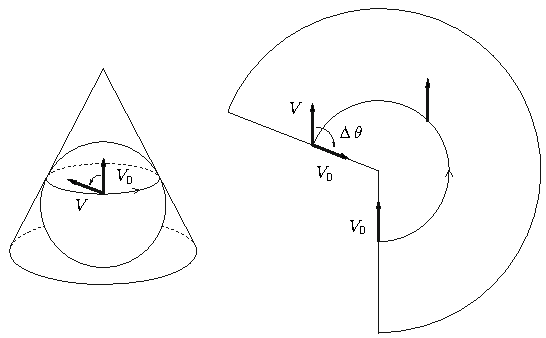
\includegraphics[width=.54\textwidth]{figures/parallel-transport-sphere.pdf}
  \caption{沿球面上一个圆的平行移动}\label{fig:sphere-circle-parallel-transport}
\end{figure}
\item 若 $c:I\to M$ 是测地线, 则 $\langle\dot c(t),X_{c(t)}\rangle$ 是常数.
\end{enumerate}

\item\label{ex:riemannian-divergence-trace}
回顾一下, 若 $M$ 是带有体积元 $\omega\in\Omega^n(M)$ 的定向微分流形, 则 $X$ 的\textbf{散度}是满足
\[
  L_X\omega=(\operatorname{div}(X))\omega
\]
的函数 $\operatorname{div}(X)$ [参见 Chapter~\RiemannSourceRef{chap:differential-forms} 的 Exercise~\RiemannSourceRef{ex:divergence-of-vector-field}]. 假设 $M$ 带有 Riemann 度量, 且 $\omega$ 是 Riemann 体积元. 证明: 在每一点 $p\in M$, 都有
\[
  \operatorname{div}(X)=\sum_{i=1}^n\langle\nabla_{Y_i}X,Y_i\rangle,
\]
其中 $\{Y_1,\ldots,Y_n\}$ 是 $T_pM$ 的一个标准正交基, $\nabla$ 是 Levi-Civita 联络.
\end{enumerate}

\end{RiemannExercise}
\endgroup

\section{测地线的最短性}\label{sec:minimizing-properties-of-geodesics}

设 $M$ 是带有仿射联络 $\nabla$ 的可微流形. 如第~\ref{sec:affine-connections}~节所见, 给定点 $p\in M$ 和切向量 $v\in T_pM$, 存在唯一的测地线 $c_v:I\to M$, 定义在极大开区间 $I\subset\mathbb{R}$ 上, 使得 $0\in I$, $c_v(0)=p$ 且 $\dot c_v(0)=v$. 现考虑由 $\gamma(t)=c_v(at)$ 定义的曲线 $\gamma:J\to M$, 其中 $a\in\mathbb{R}$, 而 $J$ 是映射 $t\mapsto at$ 下 $I$ 的原像. 有
\[
  \dot\gamma(t)=a\dot c_v(at),
\]
从而
\[
  \nabla_{\dot\gamma}\dot\gamma
  =\nabla_{a\dot c_v}(a\dot c_v)=a^2\nabla_{\dot c_v}\dot c_v=0.
\]
所以 $\gamma$ 也是测地线. 由于 $\gamma(0)=c_v(0)=p$ 且 $\dot\gamma(0)=a\dot c_v(0)=av$, $\gamma$ 就是初速度为 $av\in T_pM$ 的唯一测地线 (即 $\gamma=c_{av}$). 因此对所有 $t\in I$, 有 $c_{av}(t)=c_v(at)$. 这一性质有时称为\textbf{测地线的齐次性}. 注意, 取 $a$ 足够小, 就可以使区间 $J$ 任意大. 若 $1\in I$, 定义 $\exp_p(v)=c_v(1)$. 由测地线的齐次性, 可以对 $T_pM$ 中原点的某个开邻域 $U$ 内的 $v$ 定义 $\exp_p(v)$. 由此得到的映射 $\exp_p:U\subset T_pM\to M$ 称为 $p$ 处的\textbf{指数映射} (Fig.~\ref{fig:exponential-map}).
\RGfigure[.53\textwidth]{exponential-map}{指数映射}

\begin{RiemannProposition}\label{prop:exponential-map-local-diffeomorphism}
存在包含原点的开集 $U\subset T_pM$, 使 $\exp_p:U\to M$ 是到某个包含 $p$ 的开集 $V\subset M$ 的微分同胚 ($V$ 称为\textbf{正规邻域}).
\end{RiemannProposition}

\begin{RiemannProof}
由常微分方程的解对初始数据的光滑依赖性 (参见 \RGcite{ch03-Arn92}), 指数映射显然可微. 若 $v\in T_pM$ 使 $\exp_p(v)$ 有定义, 则由齐次性有 $\exp_p(tv)=c_{tv}(1)=c_v(t)$. 因而
\[
  (\mathrm{d}\exp_p)_0v=\left.\frac{\mathrm{d}}{\mathrm{d}t}\exp_p(tv)\right|_{t=0}
  =\left.\frac{\mathrm{d}}{\mathrm{d}t}c_v(t)\right|_{t=0}=v.
\]
因此 $(\mathrm{d}\exp_p)_0:T_0(T_pM)\cong T_pM\to T_pM$ 是恒等映射. 由反函数定理, $\exp_p$ 是从 $0\in T_pM$ 的某个开邻域 $U$ 到包含 $p=\exp_p(0)$ 的某个开集 $V\subset M$ 的微分同胚.
\end{RiemannProof}

\begin{RiemannExample}\label{ex:exponential-map-of-standard-sphere}
考虑带标准度量的 $S^2$ 上的 Levi-Civita 联络, 设 $p\in S^2$. 则 $\exp_p(v)$ 对所有 $v\in T_pS^2$ 都有定义, 但它不是微分同胚, 因为显然它不是单射. 然而, 它在开球 $B_\pi(0)\subset T_pS^2$ 上的限制是到 $S^2\setminus\{-p\}$ 的微分同胚.
\end{RiemannExample}

现在设 $(M,\langle\cdot,\cdot\rangle)$ 是 Riemann 流形, $\nabla$ 是其 Levi-Civita 联络. 由于 $\langle\cdot,\cdot\rangle$ 在 $T_pM$ 上定义了一个内积, 可以把 $T_pM$ 看作 Euclidean $n$ 维空间 $\mathbb{R}^n$. 设 $E$ 是在 $T_pM\setminus\{0\}$ 上由下式定义的向量场:
\[
  E_v=\frac{v}{\lVert v\rVert},
\]
并在 $V\setminus\{p\}$ 上定义 $X:=(\exp_p)_*E$, 其中 $V\subset M$ 是一个正规邻域. 有
\begin{align*}
  X_{\exp_p(v)}&=(\mathrm{d}\exp_p)_vE_v
   =\left.\frac{\mathrm{d}}{\mathrm{d}t}\exp_p\left(v+t\frac{v}{\lVert v\rVert}\right)\right|_{t=0}\\
  &=\left.\frac{\mathrm{d}}{\mathrm{d}t}c_v\left(1+\frac{t}{\lVert v\rVert}\right)\right|_{t=0}
   =\frac{1}{\lVert v\rVert}\dot c_v(1).
\end{align*}
由于 $\lVert\dot c_v(1)\rVert=\lVert\dot c_v(0)\rVert=\lVert v\rVert$, 可知 $X_{\exp_p(v)}$ 是测地线 $c_v$ 的单位切向量. 特别地, $X$ 必须满足
\[
  \nabla_XX=0.
\]
对使 $\overline{B_\varepsilon(0)}\subset U:=\exp_p^{-1}(V)$ 的 $\varepsilon>0$, 将以 $p$ 为中心, 半径为 $\varepsilon$ 的\phantomsection\label{idx:normal-balls}\textbf{正规球}定义为开集 $B_\varepsilon(p):=\exp_p(B_\varepsilon(0))$, 将以 $p$ 为中心, 半径为 $\varepsilon$ 的\textbf{正规球面}定义为紧子流形 $S_\varepsilon(p):=\exp_p(\partial B_\varepsilon(0))$. 现在证明 $X$ (从而经过 $p$ 的测地线) 与正规球面正交. 为此, 选取局部参数化 $\varphi:W\subset\mathbb{R}^{n-1}\to S^{n-1}\subset T_pM$, 并借此定义参数化 $\widetilde\varphi:(0,+\infty)\times W\to T_pM$:
\[
  \widetilde\varphi(r,\theta^1,\ldots,\theta^{n-1})=r\varphi(\theta^1,\ldots,\theta^{n-1})
\]
(从而 $(r,\theta^1,\ldots,\theta^{n-1})$ 是 $T_pM$ 上的球坐标). 注意
\[
  \frac{\partial}{\partial r}=E,
\]
因为
\[
  E_{\widetilde\varphi(r,\theta)}=E_{r\varphi(\theta)}
  =\varphi(\theta)=\frac{\partial\widetilde\varphi}{\partial r}(r,\theta),
\]
所以
\begin{equation}\label{eq:radial-field-in-normal-ball}
  X=(\exp_p)_*\frac{\partial}{\partial r}.
\end{equation}
由于 $\frac{\partial}{\partial\theta^i}$ 与 $\{r=\varepsilon\}$ 相切, 向量场
\begin{equation}\label{eq:angular-field-in-normal-ball}
  Y_i:=(\exp_p)_*\frac{\partial}{\partial\theta^i}
\end{equation}
与 $S_\varepsilon(p)$ 相切. 还注意到, $\bigl\lVert\frac{\partial}{\partial\theta^i}\bigr\rVert
=\bigl\lVert\frac{\partial\widetilde\varphi}{\partial\theta^i}\bigr\rVert
=r\bigl\lVert\frac{\partial\varphi}{\partial\theta^i}\bigr\rVert$ 与 $r$ 成正比. 因而当 $r\to0$ 时, $\frac{\partial}{\partial\theta^i}\to0$, 这就意味着当 $q\to p$ 时, $(Y_i)_q\to0_p$. 由于 $\exp_p$ 是局部微分同胚, 向量场 $X$ 和 $Y_i$ 在每一点都线性无关. 此外,
\[
  [X,Y_i]=\left[(\exp_p)_*\frac{\partial}{\partial r},(\exp_p)_*\frac{\partial}{\partial\theta^i}\right]
  =(\exp_p)_*\left[\frac{\partial}{\partial r},\frac{\partial}{\partial\theta^i}\right]=0
\]
[参见第~\ref{chap:differentiable-manifolds}~章的 Exercise~\ref{ex:vector-fields}(\ref{ex:pushforward-preserves-lie-bracket})]. 又因 Levi-Civita 联络对称, 等价地有
\[
  \nabla_XY_i=\nabla_{Y_i}X.
\]
为证明 $X$ 与正规球面 $S_\varepsilon(p)$ 正交, 只需证明 $X$ 与每个向量场 $Y_i$ 正交. 事实上, 由于 $\nabla_XX=0$ 和 $\lVert X\rVert=1$, 有
\begin{align*}
  X\cdot\langle X,Y_i\rangle
  &=\langle\nabla_XX,Y_i\rangle+\langle X,\nabla_XY_i\rangle\\
  &=\langle X,\nabla_{Y_i}X\rangle=\frac12Y_i\cdot\langle X,X\rangle=0,
\end{align*}
因而 $\langle X,Y_i\rangle$ 沿每条经过 $p$ 的测地线为常数. 所以
\[
  \langle X,Y_i\rangle(\exp_p v)
  =\bigl\langle X_{\exp_p(v)},(Y_i)_{\exp_p(v)}\bigr\rangle
  =\lim_{t\to0}\bigl\langle X_{\exp_p(tv)},(Y_i)_{\exp_p(tv)}\bigr\rangle=0
\]
(因为 $\lVert X\rVert=1$, 且当 $q\to p$ 时, $(Y_i)_q\to0_p$). 所以经过 $p$ 的每条测地线都与所有以 $p$ 为中心的正规球面正交. 利用这一点, 得到以下结果.

\begin{RiemannProposition}\label{prop:length-bound-from-normal-sphere}
设 $\gamma:[0,1]\to M$ 是可微曲线, 满足 $\gamma(0)=p$ 和 $\gamma(1)\in S_\varepsilon(p)$, 其中 $S_\varepsilon(p)$ 是正规球面. 则 $l(\gamma)\geq\varepsilon$, 且 $l(\gamma)=\varepsilon$ 当且仅当 $\gamma$ 是一条重参数化的测地线.
\end{RiemannProposition}

\begin{RiemannProof}
可以假设对所有 $t\in(0,1)$ 均有 $\gamma(t)\ne p$, 否则很容易构造曲线 $\widetilde\gamma:[0,1]\to M$, 满足 $\widetilde\gamma(0)=p$, $\widetilde\gamma(1)=\gamma(1)\in S_\varepsilon(p)$ 和 $l(\widetilde\gamma)<l(\gamma)$. 同理, 可假设 $\gamma([0,1))\subset B_\varepsilon(p)$. 于是可以写成
\[
  \gamma(t):=\exp_p(r(t)n(t)),
\]
其中对 $t\in(0,1]$, $r(t)\in(0,\varepsilon]$ 和 $n(t)\in S^{n-1}$ 都有定义. 注意, $r(t)$ 可以延拓为 $[0,1]$ 上的光滑函数. 于是
\[
  \dot\gamma(t)=(\exp_p)_*(\dot r(t)n(t)+r(t)\dot n(t)).
\]
由于 $\langle n(t),n(t)\rangle=1$, 有 $\langle\dot n(t),n(t)\rangle=0$, 所以 $\dot n(t)$ 与 $\partial B_{r(t)}(0)$ 相切. 注意到 $n(t)=\bigl(\frac{\partial}{\partial r}\bigr)_{r(t)n(t)}$, 得到
\[
  \dot\gamma(t)=\dot r(t)X_{\gamma(t)}+Y(t),
\]
其中 $X=(\exp_p)_*\frac{\partial}{\partial r}$, 而 $Y(t)=r(t)(\exp_p)_*\dot n(t)$ 与 $S_{r(t)}(p)$ 相切, 因而与 $X_{\gamma(t)}$ 正交. 所以
\begin{align*}
  l(\gamma)
  &=\int_0^1\bigl\langle\dot r(t)X_{\gamma(t)}+Y(t),\dot r(t)X_{\gamma(t)}+Y(t)\bigr\rangle^{\frac12}\,\mathrm{d}t\\
  &=\int_0^1\left(\dot r(t)^2+\lVert Y(t)\rVert^2\right)^{\frac12}\,\mathrm{d}t\\
  &\geq\int_0^1\dot r(t)\,\mathrm{d}t=r(1)-r(0)=\varepsilon.
\end{align*}
显然, $l(\gamma)=\varepsilon$ 当且仅当对所有 $t\in[0,1]$ 有 $\lVert Y(t)\rVert\equiv0$ 和 $\dot r(t)\geq0$. 在这种情况下, $\dot n(t)=0$ (从而 $n$ 为常量), 而 $\gamma(t)=\exp_p(r(t)n)=c_{r(t)n}(1)=c_n(r(t))$ 在相差重参数化的意义下, 是通过 $p$ 且初始条件为 $n\in T_pM$ 的测地线.
\end{RiemannProof}

\begin{RiemannDefinition}\label{def:piecewise-differentiable-curve}
\textbf{分段可微曲线}是一个连续映射 $c:[a,b]\to M$, 存在 $a=t_0<t_1<\cdots<t_{n-1}<t_n=b$, 使得对 $i=1,\ldots,n$, $c$ 在 $[t_{i-1},t_i]$ 上的限制可微. 若 $c(a)=p$ 且 $c(b)=q$, 则称 $c$ \textbf{连接} $p\in M$ 和 $q\in M$.
\end{RiemannDefinition}

分段可微曲线的\textbf{长度}没有定义上的困难. 显然, 若现在允许分段可微的重参数化, Proposition~\ref{prop:length-bound-from-normal-sphere} 很容易推广到分段可微曲线. 利用 Proposition~\ref{prop:length-bound-from-normal-sphere} 的这一推广, 指数映射的性质以及长度在重参数化下的不变性, 容易证明以下结果.

\begin{RiemannTheorem}\label{thm:radial-geodesic-minimizes-length}
设 $(M,\langle\cdot,\cdot\rangle)$ 是 Riemann 流形, $p\in M$, 且 $B_\varepsilon(p)$ 是以 $p$ 为中心的正规球. 则对每一点 $q\in B_\varepsilon(p)$, 存在连接 $p$ 到 $q$ 的测地线 $c:I\to M$. 此外, 若 $\gamma:J\to M$ 是连接 $p$ 到 $q$ 的任意其他分段可微曲线, 则 $l(\gamma)\geq l(c)$, 且 $l(\gamma)=l(c)$ 当且仅当 $\gamma$ 是 $c$ 的重参数化.\hfill\openbox
\end{RiemannTheorem}

反过来, 有如下结论.

\begin{RiemannTheorem}\label{thm:length-minimizer-is-geodesic}
设 $(M,\langle\cdot,\cdot\rangle)$ 是 Riemann 流形, $p,q\in M$. 若 $c:I\to M$ 是连接 $p$ 到 $q$ 的一条分段可微曲线, 且对连接 $p$ 到 $q$ 的任意分段可微曲线 $\gamma:J\to M$, 都有 $l(c)\leq l(\gamma)$, 则 $c$ 是一条重参数化的测地线.
\end{RiemannTheorem}

\begin{RiemannProof}
为证明本定理, 需要以下定义.

\begin{RiemannDefinition}\label{def:totally-normal-neighborhood}
若存在 $\varepsilon>0$, 使得对所有 $p\in V$ 均有 $V\subset B_\varepsilon(p)$, 则称正规邻域 $V\subset M$ 为\textbf{全正规邻域}.
\end{RiemannDefinition}

现在证明全正规邻域总是存在. 为此, 回顾 $M$ 上的局部坐标 $(x^1,\ldots,x^n)$ 给出 $TM$ 上的局部坐标 $(x^1,\ldots,x^n,v^1,\ldots,v^n)$, 它们标记向量
\[
  v^1\frac{\partial}{\partial x^1}+\cdots+v^n\frac{\partial}{\partial x^n}.
\]
测地线方程
\[
  \ddot x^i+\sum_{j,k=1}^n\Gamma_{jk}^i\dot x^j\dot x^k=0\quad(i=1,\ldots,n),
\]
对应于一阶常微分方程组
\[
  \begin{cases}
    \dot x^i=v^i\\
    \dot v^i=-\sum_{j,k=1}^n\Gamma_{jk}^iv^jv^k
  \end{cases}
  \qquad(i=1,\ldots,n).
\]
这些方程定义了向量场 $X\in\mathfrak{X}(TM)$ 的局部流, 这个向量场在局部坐标下为
\[
  X=\sum_{i=1}^n v^i\frac{\partial}{\partial x^i}
  -\sum_{i,j,k=1}^n\Gamma_{jk}^iv^jv^k\frac{\partial}{\partial v^i},
\]
称为\textbf{测地流}. 如第~\ref{chap:differentiable-manifolds}~章所见, 对每个点 $v\in TM$, 存在开邻域 $W\subset TM$ 和包含 0 的开区间 $I\subset\mathbb{R}$, 使得 $X$ 的局部流 $F:W\times I\to TM$ 有良好定义. 特别地, 对每一点 $p\in M$ 可以选取包含 $p$ 的开邻域 $U$ 和 $\varepsilon>0$, 使得测地流在 $W\times I$ 上有良好定义, 其中
\[
  W=\{v\in T_qM\mid q\in U,\ \lVert v\rVert<\varepsilon\}.
\]
利用测地线的齐次性, 使 $\varepsilon$ 足够小, 就可以使区间 $I$ 任意大. 因此, 对足够小的 $\varepsilon$, 可以用 $G(v):=(q,\exp_q(v))$ 定义映射 $G:W\to M\times M$. 由于 $\exp_q(0)=q$, $(\mathrm{d}G)_0$ 在上述局部坐标下的矩阵表示为 $\bigl(\begin{smallmatrix}I&0\\I&I\end{smallmatrix}\bigr)$, 因而 $G$ 是局部微分同胚. 必要时缩小 $U$ 和 $\varepsilon$, 就可假设 $G$ 是到其像 $G(W)$ 的微分同胚, 而该像包含点 $(p,p)=G(0_p)$. 取 $p$ 的开邻域 $V$, 使 $V\times V\subset G(W)$, 则 $V$ 显然是全正规邻域: 对每个 $q\in V$, 有 $\{q\}\times\exp_q(B_\varepsilon(0))=G(W)\cap(\{q\}\times M)\supset\{q\}\times V$, 即 $\exp_q(B_\varepsilon(0))\supset V$.

注意, 给定全正规邻域 $V$ 中任意两点 $p,q$, 存在连接 $p$ 到 $q$ 的测地线 $c:I\to M$, 使得任意其他连接 $p$ 到 $q$ 的分段可微曲线 $\gamma:J\to M$ 都满足 $l(\gamma)\geq l(c)$ (且 $l(\gamma)=l(c)$ 当且仅当 $\gamma$ 是 $c$ 的重参数化). 现在, Theorem~\ref{thm:length-minimizer-is-geodesic} 的证明由以下观察直接得到: 若 $c:I\to M$ 是连接 $p$ 到 $q$ 的分段可微曲线, 且对连接 $p$ 到 $q$ 的任意曲线 $\gamma:J\to M$ 均有 $l(c)\leq l(\gamma)$, 则 $c$ 在它所经过的每个全正规邻域内必是一条重参数化的测地线.
\end{RiemannProof}

\begin{RiemannExercise}\label{ex:minimizing-properties-of-geodesics}
\begin{enumerate}[label=(\arabic*),ref=\arabic*,leftmargin=*]
\item\label{ex:unit-gradient-integral-curves} 设 $(M,g)$ 是 Riemann 流形, $f:M\to\mathbb{R}$ 是光滑函数. 若 $\lVert\operatorname{grad}(f)\rVert\equiv1$, 则 $\operatorname{grad}(f)$ 的积分曲线是测地线. 分别利用下列两种方法证明:
\begin{enumerate}[label=(\alph*),leftmargin=*]
\item 测地线的定义;
\item 测地线的最短性.
\end{enumerate}
\item\label{ex:metric-and-connection-in-normal-coordinates} 设 $M$ 是 Riemann 流形, $\nabla$ 是 $M$ 上的 Levi–Civita 联络. 给定 $p\in M$ 和 $T_pM$ 的一组基 $\{v_1,\ldots,v_n\}$, 考虑正规邻域的参数化 $\varphi:U\subset\mathbb{R}^n\to M$, 它由
\[
  \varphi(x^1,\ldots,x^n)=\exp_p(x^1v_1+\cdots+x^nv_n)
\]
给出 (局部坐标 $(x^1,\ldots,x^n)$ 称为\textbf{正规坐标}). 证明:
\begin{enumerate}[label=(\alph*),leftmargin=*]
\item 在这些坐标下, $\Gamma_{jk}^i(p)=0$ {\small (\textbf{提示:} 考虑测地线方程)};
\item 若 $\{v_1,\ldots,v_n\}$ 是标准正交基, 则 $g_{ij}(p)=\delta_{ij}$.
\end{enumerate}
\item\label{ex:bi-invariant-metrics-on-lie-groups} 设 $G$ 是配备\textbf{双不变 Riemann 度量}的 Lie 群 (即对所有 $g\in G$, $L_g$ 和 $R_g$ 都是等距映射), 并设 $i:G\to G$ 是由 $i(g)=g^{-1}$ 定义的微分同胚.
\begin{enumerate}[label=(\alph*),leftmargin=*]
\item 计算 $(\mathrm{d}i)_e$, 并证明对所有 $g\in G$, 有
\[
  (\mathrm{d}i)_g=(\mathrm{d}R_{g^{-1}})_e(\mathrm{d}i)_e(\mathrm{d}L_{g^{-1}})_g.
\]
由此推得 $i$ 是等距映射.
\item 设 $v\in\mathfrak{g}=T_eG$, $c_v$ 是满足 $c_v(0)=e$ 和 $\dot c_v(0)=v$ 的测地线. 证明若 $t$ 足够小, 则 $c_v(-t)=(c_v(t))^{-1}$. 由此推得 $c_v$ 在 $\mathbb{R}$ 上有定义, 且对所有 $t,s\in\mathbb{R}$ 满足 $c_v(t+s)=c_v(t)c_v(s)$.
{\small (\textbf{提示:} 回顾全正规邻域中的任意两点由该邻域内唯一一条测地线连接).}
\item \phantomsection\label{idx:bi-invariant-metric-geodesics}证明 $G$ 的测地线是左不变向量场的积分曲线, 并证明映射 $\exp$ (Lie 群的指数映射) 和 $\exp_e$ (单位元处的测地指数映射) 一致.
\item 设 $\nabla$ \phantomsection\label{idx:bi-invariant-metric-levi-civita}是双不变度量的 Levi-Civita 联络, $X,Y$ 是两个左不变向量场. 证明
\[
  \nabla_XY=\frac12[X,Y].
\]
\item 核实 Exercise~\ref{ex:riemannian-manifolds}(\ref{ex:left-invariant-metric}) 中的左不变度量实际上是双不变的.
\item 证明任意紧 Lie 群都容许双不变度量.
{\small (\textbf{提示:} 将一个左不变度量对所有右平移取平均).}
\end{enumerate}
\item\label{ex:isometries-send-geodesics-to-geodesics} 利用 Theorem~\ref{thm:length-minimizer-is-geodesic} 证明: 若 $f:M\to N$ 是等距映射且 $c:I\to M$ 是测地线, 则 $f\circ c:I\to N$ 也是测地线.
\item\label{ex:fixed-point-submanifold-of-isometry} 设 $f:M\to M$ 是等距映射, 其不动点集合是连通的 1 维子流形 $N\subset M$. 证明 $N$ 是一条测地线的像.
\item\label{ex:jacobi-fields-and-cut-locus} 设 $(M,\langle\cdot,\cdot\rangle)$ 是 Riemann 流形, 其测地线可以延拓到参数的所有取值. 设 $p\in M$.
\begin{enumerate}[label=(\alph*),leftmargin=*]
\item 设 $X$ 和 $Y_i$ 是以 $p$ 为中心的正规球上由 \eqref{eq:radial-field-in-normal-ball} 和 \eqref{eq:angular-field-in-normal-ball} 定义的向量场. 证明 $Y_i$ 满足 \textbf{Jacobi 方程}
\[
  \nabla_X\nabla_XY_i=R(X,Y_i)X,
\]
其中由
\[
  R(X,Y)Z=\nabla_X\nabla_YZ-\nabla_Y\nabla_XZ-\nabla_{[X,Y]}Z,
\]
定义的 $R:\mathfrak{X}(M)\times\mathfrak{X}(M)\times\mathfrak{X}(M)\to\mathfrak{X}(M)$ 称为\textbf{曲率算子} (参见第~\RGref{chap:curvature}~章).
{\small (\textbf{Remark:} 可以证明 $(R(X,Y)Z)_p$ 只依赖于 $X_p,Y_p,Z_p$).}
\item 考虑满足 $c(0)=p$ 的弧长参数化测地线 $c:\mathbb{R}\to M$. 若沿 $c$ 的向量场 $Y$ 满足沿 $c$ 的 Jacobi 方程
\[
  \frac{D^2Y}{\mathrm{d}t^2}=R(\dot c,Y)\dot c,
\]
则称它为 \textbf{Jacobi 场}. 证明 $Y$ 是满足 $Y(0)=0$ 的 Jacobi 场当且仅当
\[
  Y(t)=\left.\frac{\partial}{\partial s}\exp_p(tv(s))\right|_{s=0}
\]
其中 $v:(-\varepsilon,\varepsilon)\to T_pM$ 满足 $v(0)=\dot c(0)$.
\item 若点 $q\in M$ 是 $\exp_p$ 的临界值, 则称 $q$ \textbf{共轭于} $p$. 证明 $q$ 共轭于 $p$ 当且仅当存在一个非零 Jacobi 场 $Y$, 它沿着连接 $p=c(0)$ 和 $q=c(b)$ 的测地线 $c$ 且满足 $Y(0)=Y(b)=0$. 由此推知, 若 $q$ 共轭于 $p$, 则 $p$ 共轭于 $q$.
\item 若对所有 $X,Y\in\mathfrak{X}(M)$ 都有 $\langle R(X,Y)X,Y\rangle\geq0$, 则称流形 $M$ 具有\textbf{非正曲率}. 证明在这样的流形上没有两点共轭.
\item 给定一条由弧长参数化且满足 $c(0)=p$ 的测地线 $c:I\to M$, 设 $t_c$ 为使 $c$ 是连接 $p$ 到 $c(t)$ 的最短曲线的 $t$ 值所成集合的上确界 (因此 $t_c>0$). 定义 $p$ 的\textbf{割迹}为所有形如 $c(t_c)$ 且 $t_c<+\infty$ 的点所成的集合. 当 $M$ 分别为以下流形时, 求给定点 $p\in M$ 的割迹:
\begin{enumerate}[label=(\roman*),leftmargin=*]
\item 带平直方形度量的环面 $T^n$;
\item 带标准度量的球面 $S^n$;
\item 带标准度量的射影空间 $\mathbb{R}P^n$.
\end{enumerate}
在这些例子中验证: 割迹中的任一点或者共轭于 $p$, 或者由两条长度相同但像不同的测地线与 $p$ 相连.
{\small (\textbf{Remark:} 这是割迹的一般性质, 证明见 \RGcite{ch03-dC93} 或 \RGcite{ch03-GHL04}).}
\end{enumerate}
\end{enumerate}
\end{RiemannExercise}

\section{Hopf-Rinow 定理}\label{sec:hopf-rinow-theorem}

设 $(M,g)$ 是 Riemann 流形. 全正规邻域的存在性蕴含, 总可以用一条最短测地线连接两个充分接近的点 $p,q\in M$. 现在从整体上讨论同一问题.

\begin{RiemannExample}\label{ex:global-geodesics-of-euclidean-space-and-sphere}
\begin{enumerate}[label=(\arabic*),leftmargin=*]
\item 给定两个不同的点 $p,q\in\mathbb{R}^n$, 对 Euclidean 度量存在唯一一条连接这两点的测地线 (在相差重参数化的意义下).
\item 给定两个不同的点 $p,q\in S^n$, 对标准度量至少存在两条连接这两点的测地线, 它们互不为重参数化.
\item 若 $p\ne0$, 则对 $\mathbb{R}^n\setminus\{0\}$ 中的 Euclidean 度量, 不存在从 $p$ 到 $-p$ 的测地线.
\end{enumerate}
\end{RiemannExample}

在许多情形下 (例如 $\mathbb{R}^n\setminus\{0\}$), 存在不能延拓到参数的所有取值的测地线. 换言之, $\exp_p(v)$ 并非对所有 $v\in T_pM$ 都有定义.

\begin{RiemannDefinition}\label{def:geodesic-completeness}
若对每个点 $p\in M$, 映射 $\exp_p$ 都在 $T_pM$ 上有定义, 则称 Riemann 流形 $(M,\langle\cdot,\cdot\rangle)$ \textbf{测地完备}.
\end{RiemannDefinition}

连通 Riemann 流形还有另一种完备性概念, 源于任何这样的流形自然地是一个度量空间.

\begin{RiemannDefinition}\label{def:riemannian-distance}
设 $(M,\langle\cdot,\cdot\rangle)$ 是连通 Riemann 流形, 且 $p,q\in M$. $p$ 与 $q$ 之间的\textbf{距离}定义为
\[
  d(p,q)=\inf\{l(\gamma)\mid\text{$\gamma$ 是从 $p$ 到 $q$ 的分段可微曲线}\}.
\]
\end{RiemannDefinition}

注意, 若存在连接 $p$ 到 $q$ 的最短测地线 $c$, 则 $d(p,q)=l(c)$. 如下述命题所述, 函数 $d:M\times M\to[0,+\infty)$ 确实是一个距离.

\begin{RiemannProposition}\label{prop:riemannian-distance-defines-metric-topology}
$(M,d)$ 是度量空间, 即对所有 $p,q,r\in M$, $d$ 满足:
\begin{enumerate}[label=(\roman*),leftmargin=*]
\item \textbf{正性:} $d(p,q)\geq0$, 且 $d(p,q)=0$ 当且仅当 $p=q$;
\item \textbf{对称性:} $d(p,q)=d(q,p)$;
\item \textbf{三角不等式:} $d(p,r)\leq d(p,q)+d(q,r)$.
\end{enumerate}
$M$ 上诱导的度量空间拓扑与 $M$ 作为可微流形的拓扑一致.
\end{RiemannProposition}

\begin{RiemannProof}
见 Exercise~\ref{ex:hopf-rinow-theorem}(\ref{ex:proof-of-riemannian-metric-space-topology}).
\end{RiemannProof}

因此, 可以讨论作为度量空间的 $M$ 的完备性 (即 Cauchy 序列是否收敛). 完备与测地完备等价, 这就是下述定理的内容.

\begin{RiemannTheorem}[Hopf-Rinow]\label{thm:hopf-rinow}
设 $(M,\langle\cdot,\cdot\rangle)$ 是连通 Riemann 流形, $p\in M$. 以下断言等价:
\begin{enumerate}[label=(\roman*),ref=\roman*,leftmargin=*]
\item\label{thm:hopf-rinow-geodesically-complete} $M$ 测地完备;
\item\label{thm:hopf-rinow-metrically-complete} $(M,d)$ 是完备度量空间;
\item\label{thm:hopf-rinow-exponential-at-one-point} $\exp_p$ 在 $T_pM$ 上有定义.
\end{enumerate}
此外, 若 $(M,\langle\cdot,\cdot\rangle)$ 测地完备, 则对所有 $q\in M$, 存在连接 $p$ 到 $q$ 的测地线 $c$, 满足 $l(c)=d(p,q)$.
\end{RiemannTheorem}

\begin{RiemannProof}
显然 (\ref{thm:hopf-rinow-geodesically-complete}) $\Rightarrow$ (\ref{thm:hopf-rinow-exponential-at-one-point}).

首先证明若 (\ref{thm:hopf-rinow-exponential-at-one-point}) 成立, 则对所有 $q\in M$, 存在连接 $p$ 到 $q$ 的测地线 $c$, 满足 $l(c)=d(p,q)$. 设 $d(p,q)=\rho$. 若 $\rho=0$, 则 $q=p$, 无需证明. 若 $\rho>0$, 取 $\varepsilon\in(0,\rho)$ 使 $S_\varepsilon(p)$ 是一个正规球面 (它是 $M$ 的一个紧子流形). 于是连续函数 $x\mapsto d(x,q)$ 有一个最小值点 $x_0\in S_\varepsilon(p)$. 此外, $x_0=\exp_p(\varepsilon v)$, 其中 $\lVert v\rVert=1$. 考虑测地线 $c_v(t)=\exp_p(tv)$. 将证明 $q=c_v(\rho)$. 为此, 考虑集合
\[
  A=\{t\in[0,\rho]\mid d(c_v(t),q)=\rho-t\}.
\]
由于映射 $t\mapsto d(c_v(t),q)$ 连续, $A$ 是闭集. 此外, $A\ne\varnothing$, 因为显然 $0\in A$. 现在证明任何点 $t_0\in[0,\rho)$ 都不可能是 $A$ 的最大值. 这蕴含 $A$ 的最大值必为 $\rho$ (因而 $d(c_v(\rho),q)=0$, 即 $c_v(\rho)=q$, 所以 $c_v$ 连接 $p$ 到 $q$, 且 $l(c_v)=\rho$). 取 $t_0\in A\cap[0,\rho)$, $r=c_v(t_0)$, 并取 $\delta\in(0,\rho-t_0)$ 使 $S_\delta(r)$ 为正规球面. 设 $y_0$ 是连续函数 $y\mapsto d(y,q)$ 在紧集 $S_\delta(r)$ 上的一个最小值点 (Fig.~\ref{fig:hopf-rinow-proof}). 将证明 $y_0=c_v(t_0+\delta)$. 事实上, 有
\RGfigure[.55\textwidth]{hopf-rinow-proof}{Hopf-Rinow 定理的证明}
\[
  \rho-t_0=d(r,q)=\delta+\min_{y\in S_\delta(r)}d(y,q)=\delta+d(y_0,q),
\]
所以
\begin{equation}\label{eq:distance-from-minimum-on-normal-sphere}
  d(y_0,q)=\rho-t_0-\delta.
\end{equation}
由三角不等式得到
\[
  d(p,y_0)\geq d(p,q)-d(y_0,q)=\rho-(\rho-t_0-\delta)=t_0+\delta,
\]
而沿 $c_v$ 从 $p$ 到 $r$, 再沿测地线从 $r$ 到 $y_0$ 的分段可微曲线, 长度为 $t_0+\delta$. 因此它是最短曲线, 从而是一条 (重参数化的) 测地线. 如前所述, 得 $y_0=c_v(t_0+\delta)$. 因此, 由 \eqref{eq:distance-from-minimum-on-normal-sphere} 可写成
\[
  d(c_v(t_0+\delta),q)=\rho-(t_0+\delta),
\]
这意味着 $t_0+\delta\in A$, 所以 $t_0$ 不可能是 $A$ 的最大值.

现在证明 (\ref{thm:hopf-rinow-exponential-at-one-point}) $\Rightarrow$ (\ref{thm:hopf-rinow-metrically-complete}). 先证明任何有界闭子集 $K\subset M$ 都紧. 事实上, 若 $K$ 有界, 则对某个 $R>0$, 有 $K\subset B_R(p)$, 其中
\[
  B_R(p)=\{q\in M\mid d(p,q)<R\}.
\]
如前所见, $p$ 可由长度小于 $R$ 的测地线连接到 $B_R(p)$ 中任意一点, 因而 $B_R(p)\subset\exp_p\bigl(\overline{B_R(0)}\bigr)$. 由于 $\exp_p:T_pM\to M$ 连续且 $\overline{B_R(0)}$ 紧, 集合 $\exp_p\bigl(\overline{B_R(0)}\bigr)$ 也紧. 因此 $K$ 是紧集的闭子集, 从而 $K$ 紧. 现在, 若 $\{p_n\}$ 是 $M$ 中的一个 Cauchy 序列, 则其闭包有界, 从而紧. 因此 $\{p_n\}$ 必有收敛子序列, 所以它本身必收敛.

最后证明 (\ref{thm:hopf-rinow-metrically-complete}) $\Rightarrow$ (\ref{thm:hopf-rinow-geodesically-complete}). 设 $c$ 是一条对 $t<t_0$ 有定义的测地线. 不失一般性, 可假设它已\textbf{归一化}, 即 $\lVert\dot c(t)\rVert=1$. 设 $\{t_n\}$ 是收敛到 $t_0$ 的递增实数序列. 由于 $d(c(t_m),c(t_n))\leq|t_m-t_n|$, 可知 $\{c(t_n)\}$ 是一个 Cauchy 序列. 因假设 $M$ 完备, 可知 $c(t_n)\to p\in M$, 且容易看出, 当 $t\to t_0$ 时, $c(t)\to p$. 设 $B_\varepsilon(p)$ 为以 $p$ 为中心的正规球. 则 $c$ 在此正规球内可以延拓到 $t_0$ 之后.
\end{RiemannProof}

\begin{RiemannCorollary}\label{cor:compact-riemannian-manifold-geodesically-complete}
若 $M$ 紧, 则 $M$ 测地完备.
\end{RiemannCorollary}

\begin{RiemannProof}
任何紧度量空间都完备.
\end{RiemannProof}

\begin{RiemannCorollary}\label{cor:closed-submanifold-complete-in-induced-metric}
若 $M$ 是完备连通 Riemann 流形的闭连通子流形, 并赋予诱导度量, 则 $M$ 完备.
\end{RiemannCorollary}

\begin{RiemannProof}
设 $M$ 是完备连通 Riemann 流形 $N$ 的闭连通子流形. 设 $d$ 是 $N$ 上度量确定的距离, $d^*$ 是 $M$ 上诱导度量确定的距离. 因为 $M$ 上的任何曲线也是 $N$ 上的曲线, 所以 $d\leq d^*$. 设 $\{p_n\}$ 是 $(M,d^*)$ 中的一个 Cauchy 序列. 则 $\{p_n\}$ 是 $(N,d)$ 中的 Cauchy 序列, 因而在 $N$ 中收敛到一点 $p\in M$ (因为 $N$ 完备且 $M$ 闭). 由于 $M$ 的拓扑由 $N$ 的拓扑诱导, 可知在 $M$ 上有 $p_n\to p$.
\end{RiemannProof}

\begin{RiemannExercise}\label{ex:hopf-rinow-theorem}
\begin{enumerate}[label=(\arabic*),ref=\arabic*,leftmargin=*]
\item\label{ex:proof-of-riemannian-metric-space-topology} 证明 Proposition~\ref{prop:riemannian-distance-defines-metric-topology}.
\item\label{ex:metric-ball-in-slit-plane} 考虑带 Euclidean 度量的 $\mathbb{R}^2\setminus\{(x,0)\mid-3\leq x\leq3\}$. 求 $B_7(0,4)$.
\item\label{ex:heine-borel-property-and-completeness}
\begin{enumerate}[label=(\alph*),leftmargin=*]
\item 证明连通 Riemann 流形完备当且仅当紧集就是有界闭集.
\item 给出一个含有非紧的有界闭集的连通 Riemann 流形的例子.
\end{enumerate}
\item\label{ex:completeness-of-homogeneous-manifolds} 若对任意两点 $p,q\in M$, 都存在等距映射 $f:M\to M$ 使 $f(p)=q$, 则称 Riemann 流形 $(M,\langle\cdot,\cdot\rangle)$ \textbf{齐性}. 证明:
\begin{enumerate}[label=(\alph*),leftmargin=*]
\item 任意齐性 Riemann 流形都完备;
\item 若 Lie 群 $G$ 容许双不变度量 [参见 Exercise~\ref{ex:minimizing-properties-of-geodesics}(\ref{ex:bi-invariant-metrics-on-lie-groups})], 则指数映射 $\exp:\mathfrak{g}\to G$ 是满射;
\item $SL(2,\mathbb{R})$ 不容许双不变度量.
\end{enumerate}
\item\label{ex:ambrose-and-cartan-hadamard-theorems} 设 $(M,g)$ 是完备 Riemann 流形. 证明:
\begin{enumerate}[label=(\alph*),leftmargin=*]
\item (\emph{Ambrose 定理}) 若 $(N,h)$ 是 Riemann 流形, $f:M\to N$ 是局部等距映射, 则 $f$ 是覆盖映射;
\item 存在不是覆盖映射的满局部等距映射;
\item (\emph{Cartan–Hadamard 定理}) 若 $(M,g)$ 具有非正曲率 [参见 Exercise~\ref{ex:minimizing-properties-of-geodesics}(\ref{ex:jacobi-fields-and-cut-locus})], 则对每个点 $p\in M$, 指数映射 $\exp_p:T_pM\to M$ 是覆盖映射.
{\small (\textbf{Remark:} 特别地, 若 $M$ 单连通, 则 $M$ 必与 $\mathbb{R}^n$ 微分同胚).}
\end{enumerate}
\end{enumerate}
\end{RiemannExercise}

\section{附注}\label{sec:notes-on-riemannian-manifolds}

\subsection{第 \ref{sec:hopf-rinow-theorem} 节}\label{subsec:notes-hopf-rinow}

本节用到几个关于度量空间的定义和结果, 现在来讨论它们. \textbf{度量空间}是一个二元组 $(M,d)$, 其中 $M$ 是一个集合, $d:M\times M\to[0,+\infty)$ 是满足 Proposition~\ref{prop:riemannian-distance-defines-metric-topology} 所列性质的映射. 集合
\[
  B_\varepsilon(p)=\{q\in M\mid d(p,q)<\varepsilon\}
\]
称为以 $p$ 为中心, 半径为 $\varepsilon$ 的\textbf{开球}. 所有这类球的族构成 $M$ 上一个 Hausdorff 拓扑的基, 此拓扑称为\textbf{度量拓扑}. 注意, 在此拓扑中, $p_n\to p$ 当且仅当 $d(p_n,p)\to0$. 虽然度量空间 $(M,d)$ 不一定满足第二可数性, 下述结论仍然成立: $F\subset M$ 为闭集当且仅当 $F$ 中的每个收敛序列的极限都在 $F$ 中, 而 $K\subset M$ 紧当且仅当 $K$ 中的每个序列在 $K$ 中都有子列极限.

若对所有 $\varepsilon>0$, 存在 $N\in\mathbb{N}$, 使得对所有 $m,n>N$ 都有 $d(p_n,p_m)<\varepsilon$, 则称 $M$ 中的序列 $\{p_n\}$ 为 \textbf{Cauchy 序列}. 容易看出所有收敛序列都是 Cauchy 序列. 然而反过来不一定成立 (但若一个 Cauchy 序列有收敛子序列, 则它必收敛). 若度量空间的所有 Cauchy 序列均收敛, 就称它\textbf{完备}. 完备度量空间的闭子集本身也是完备的.

若集合是某个球的子集, 就称它\textbf{有界}. 例如, Cauchy 序列所有项所成的集合有界. 容易证明, 若 $K\subset M$ 紧, 则 $K$ 必有界且闭 (但反过来不一定成立). 紧度量空间必完备.

\subsection{文献附注}\label{subsec:riemannian-manifolds-literature}

本章的材料在大多数 Riemann 几何著作中都可以找到 (例如 [\RGref{bib:ch03-Boo03}, \RGref{bib:ch03-dC93}, \RGref{bib:ch03-GHL04}]). 一般仿射联络的更多细节参见 \RGcite{KN96}. Lie 群上的双不变度量是对称空间的例子, 其优美的理论例如可见 \RGcite{Hel01}.

\RGReferenceSection

\begin{description}[style=multiline,leftmargin=5em,labelwidth=4.5em,font=\normalfont]
\item[{[Arn92]}]\RGbiblabel[ch03-]{Arn92}Arnold, V.I.: Ordinary Differential Equations. Springer, Berlin (1992)
\item[{[Boo03]}]\RGbiblabel[ch03-]{Boo03}Boothby, W.: An Introduction to Differentiable Manifolds and Riemannian Geometry. Academic Press, New York (2003)
\item[{[dC93]}]\RGbiblabel[ch03-]{dC93}do Carmo, M.: Riemannian Geometry. Birkhäuser, Boston (1993)
\item[{[GHL04]}]\RGbiblabel[ch03-]{GHL04}Gallot, S., Hulin, D., Lafontaine, J.: Riemannian Geometry. Springer, Berlin (2004)
\item[{[GR70]}]\RGbiblabel{GR70}Gromov, M., Rohlin, V.: Imbeddings and Immersions in Riemannian Geometry. Usp. Mat. Nauk \textbf{25}, 3–62 (1970)
\item[{[Hel01]}]\RGbiblabel{Hel01}Helgasson, S.: Differential Geometry, Lie Groups and Symmetric Spaces. American Mathematical Society, Providence (2001)
\item[{[KN96]}]\RGbiblabel{KN96}Kobayashi, S., Nomizu, K.: Foundations of Differential Geometry, vol. I and II. Wiley, New York (1996)
\item[{[Nas56]}]\RGbiblabel{Nas56}Nash, J.: The Imbedding Problem for Riemannian Manifolds. Ann. Math. \textbf{63}, 20–63 (1956)
\end{description}

\chapter{曲率}\label{chap:curvature}
\begingroup
\renewcommand{\thefootnote}{}
\footnotetext{\textcopyright\ Springer International Publishing Switzerland 2014.
  L. Godinho and J. Natário, \emph{An Introduction to Riemannian Geometry},
  Universitext. DOI \href{https://doi.org/10.1007/978-3-319-08666-8_4}{10.1007/978-3-319-08666-8\_4}.}
\endgroup

一般 Riemann 流形的局部几何不同于 Euclidean 空间 $\mathbb{R}^n$ 的平直几何. 例如, 2 维球面 $S^2$ (带标准度量) 上测地三角形的内角和总大于 $\pi$. 衡量这种差异的是\textbf{曲率}. 这一概念由 Gauss 在 1827 年的论文\textquotedblleft 曲面的一般研究\textquotedblright 中引入, 又由 Riemann 本人 (于 1854 年) 推广到任意 Riemann 流形. 曲率有许多不同的表现: 测地线偏离的速率, 沿不同向量场的协变导数不交换的程度, 测地三角形内角和与 $\pi$ 的差, 或者将向量沿闭曲线平行移动时该向量旋转的角度.

本章研究曲率的各种刻画和性质. 第~\RGref{sec:curvature}~节引入一般仿射联络的\textbf{曲率算子}, 对 Riemann 流形还引入等价但更具几何性的\textbf{截面曲率}概念. 本节还定义由曲率张量缩并得到的 \textbf{Ricci 曲率张量}和\textbf{标量曲率}. 在广义相对论中, 这些量是表述 Einstein 方程的基础 (第~\RGref{chap:relativity}~章).

第~\RGref{sec:cartan-structure-equations}~节建立 \textbf{Cartan 结构方程}, 这是利用微分形式计算曲率的一种有力方法. 第~\RGref{sec:gauss-bonnet-theorem}~节利用这些方程证明 \textbf{Gauss–Bonnet 定理}, 将紧曲面的曲率与其拓扑联系起来. 这一定理给出一个简单的例子, 说明完备 Riemann 流形的曲率如何制约其拓扑.

第~\RGref{sec:manifolds-of-constant-curvature}~节讨论具有常曲率的完备 Riemann 流形. 这些流形给出弯曲几何的重要例子, 包括 Gauss, Bolyai 和 Lobachevsky 的负曲率非 Euclidean 几何.

最后, 第~\RGref{sec:isometric-immersions}~节研究 Riemann 流形的曲率与其子流形 (带诱导度量) 的曲率之间的关系. 这推广了 Gauss 对曲面的研究, 包括他著名的 \emph{Theorema Egregium}.

\section{曲率}\label{sec:curvature}

如第~\ref{chap:riemannian-manifolds}~章的 Exercise~\ref{ex:levi-civita-connection}(\ref{ex:spherical-geodesics-and-transport}) 所见, 带标准度量的 2 维球面 $S^2$ 上没有任何开集与 Euclidean 平面上的一个开集等距. 从局部区分这两个 Riemann 流形的几何对象就是所谓的\textbf{曲率算子}, 它也出现在许多其他情形中 [参见第~\ref{chap:riemannian-manifolds}~章的 Exercise~\ref{ex:minimizing-properties-of-geodesics}(\ref{ex:jacobi-fields-and-cut-locus})].

\begin{RiemannDefinition}\label{def:curvature-of-connection}
联络 $\nabla$ 的\textbf{曲率} $R$ 为每对向量场 $X,Y\in\mathfrak{X}(M)$ 指派映射 $R(X,Y):\mathfrak{X}(M)\to\mathfrak{X}(M)$, 该映射由下式定义:
\[
  R(X,Y)Z=\nabla_X\nabla_YZ-\nabla_Y\nabla_XZ-\nabla_{[X,Y]}Z.
\]
\end{RiemannDefinition}

因此, $R$ 衡量联络的不交换性. 由于
\begin{enumerate}[label=(\roman*),leftmargin=*]
\item $R(fX_1+gX_2,Y)Z=fR(X_1,Y)Z+gR(X_2,Y)Z$,
\item $R(X,fY_1+gY_2)Z=fR(X,Y_1)Z+gR(X,Y_2)Z$,
\item $R(X,Y)(fZ_1+gZ_2)=fR(X,Y)Z_1+gR(X,Y)Z_2$,
\end{enumerate}
对所有向量场 $X,X_1,X_2,Y,Y_1,Y_2,Z,Z_1,Z_2\in\mathfrak{X}(M)$ 和所有光滑函数 $f,g\in C^\infty(M)$ 成立, $R$ 定义了一个称为 \textbf{Riemann 张量}的 $(3,1)$-张量. 证明留作练习 [参见 Exercise~\ref{ex:curvature}(\ref{ex:tensoriality-of-curvature})]. 在 $M$ 上选取坐标系 $x:V\to\mathbb{R}^n$, 则此张量在局部可写成
\[
  R=\sum_{i,j,k,l=1}^n R_{ijk}{}^l\,\mathrm{d}x^i\otimes\mathrm{d}x^j
  \otimes\mathrm{d}x^k\otimes\frac{\partial}{\partial x^l},
\]
其中每个系数 $R_{ijk}{}^l$ 是向量场 $R\bigl(\frac{\partial}{\partial x^i},\frac{\partial}{\partial x^j}\bigr)\frac{\partial}{\partial x^k}$ 的第 $l$ 个坐标, 即
\[
  R\left(\frac{\partial}{\partial x^i},\frac{\partial}{\partial x^j}\right)
  \frac{\partial}{\partial x^k}=\sum_{l=1}^n R_{ijk}{}^l\frac{\partial}{\partial x^l}.
\]
利用 $\bigl[\frac{\partial}{\partial x^i},\frac{\partial}{\partial x^j}\bigr]=0$, 有
\begin{align*}
  R\left(\frac{\partial}{\partial x^i},\frac{\partial}{\partial x^j}\right)
  \frac{\partial}{\partial x^k}
  &=\nabla_{\frac{\partial}{\partial x^i}}\nabla_{\frac{\partial}{\partial x^j}}
    \frac{\partial}{\partial x^k}
  -\nabla_{\frac{\partial}{\partial x^j}}\nabla_{\frac{\partial}{\partial x^i}}
    \frac{\partial}{\partial x^k}\\
  &=\nabla_{\frac{\partial}{\partial x^i}}
    \left(\sum_{m=1}^n\Gamma_{jk}^m\frac{\partial}{\partial x^m}\right)
   -\nabla_{\frac{\partial}{\partial x^j}}
    \left(\sum_{m=1}^n\Gamma_{ik}^m\frac{\partial}{\partial x^m}\right)\\
  &=\sum_{m=1}^n\left(\frac{\partial}{\partial x^i}\cdot\Gamma_{jk}^m
    -\frac{\partial}{\partial x^j}\cdot\Gamma_{ik}^m\right)\frac{\partial}{\partial x^m}\\
  &\quad+\sum_{l,m=1}^n(\Gamma_{jk}^m\Gamma_{im}^l-\Gamma_{ik}^m\Gamma_{jm}^l)
    \frac{\partial}{\partial x^l}\\
  &=\sum_{l=1}^n\left(\frac{\partial\Gamma_{jk}^l}{\partial x^i}
    -\frac{\partial\Gamma_{ik}^l}{\partial x^j}
    +\sum_{m=1}^n\Gamma_{jk}^m\Gamma_{im}^l
    -\sum_{m=1}^n\Gamma_{ik}^m\Gamma_{jm}^l\right)\frac{\partial}{\partial x^l},
\end{align*}
所以
\[
  R_{ijk}{}^l=\frac{\partial\Gamma_{jk}^l}{\partial x^i}
  -\frac{\partial\Gamma_{ik}^l}{\partial x^j}
  +\sum_{m=1}^n\Gamma_{jk}^m\Gamma_{im}^l-\sum_{m=1}^n\Gamma_{ik}^m\Gamma_{jm}^l.
\]

\begin{RiemannExample}\label{ex:curvature-of-euclidean-space}
考虑带有 Euclidean 度量及相应 Levi–Civita 联络的 $M=\mathbb{R}^n$ (即 Christoffel 符号 $\Gamma_{ij}^k\equiv0$). 此时 $R_{ijk}{}^l=0$, 曲率 $R$ 为零. 因此, 也可以把曲率解释为衡量给定流形上的联络与 Euclidean 空间的 Levi–Civita 联络有多大差异的量.
\end{RiemannExample}

若联络对称 (如 Levi–Civita 联络), 则张量 $R$ 满足所谓的 \textbf{Bianchi 恒等式}.

\begin{RiemannProposition}[Bianchi 恒等式]\label{prop:first-bianchi-identity}
若 $M$ 是带有对称联络的流形, 则相应的曲率满足
\[
  R(X,Y)Z+R(Y,Z)X+R(Z,X)Y=0.
\]
\end{RiemannProposition}

\begin{RiemannProof}
这个性质是向量场的 Jacobi 恒等式的直接推论. 事实上,
\begin{align*}
  &R(X,Y)Z+R(Y,Z)X+R(Z,X)Y\\
  &\quad=\nabla_X\nabla_YZ-\nabla_Y\nabla_XZ-\nabla_{[X,Y]}Z
   +\nabla_Y\nabla_ZX-\nabla_Z\nabla_YX-\nabla_{[Y,Z]}X\\
  &\qquad{}+\nabla_Z\nabla_XY-\nabla_X\nabla_ZY-\nabla_{[Z,X]}Y\\
  &\quad=\nabla_X(\nabla_YZ-\nabla_ZY)+\nabla_Y(\nabla_ZX-\nabla_XZ)
    +\nabla_Z(\nabla_XY-\nabla_YX)\\
  &\qquad{}-\nabla_{[X,Y]}Z-\nabla_{[Y,Z]}X-\nabla_{[Z,X]}Y,
\end{align*}
所以, 由于联络对称, 有
\begin{align*}
  &R(X,Y)Z+R(Y,Z)X+R(Z,X)Y\\
  &\quad=\nabla_X[Y,Z]+\nabla_Y[Z,X]+\nabla_Z[X,Y]
    -\nabla_{[Y,Z]}X-\nabla_{[Z,X]}Y-\nabla_{[X,Y]}Z\\
  &\quad=[X,[Y,Z]]+[Y,[Z,X]]+[Z,[X,Y]]=0.
\end{align*}
\end{RiemannProof}

以下假定 $(M,g)$ 是 Riemann 流形, $\nabla$ 是其 Levi–Civita 联络. 可以定义一个新的协变 4-张量, 称为\textbf{曲率张量}:
\[
  R(X,Y,Z,W):=g(R(X,Y)Z,W).
\]
注意, 由于度量非退化, 曲率张量与 Riemann 张量包含相同的信息. 再在 $M$ 上选取坐标系 $x:V\to\mathbb{R}^n$, 可将此张量写成
\[
  R(X,Y,Z,W)=\left(\sum_{i,j,k,l=1}^n R_{ijkl}\,\mathrm{d}x^i\otimes\mathrm{d}x^j
  \otimes\mathrm{d}x^k\otimes\mathrm{d}x^l\right)(X,Y,Z,W)
\]
其中
\begin{align*}
  R_{ijkl}
  &=g\left(R\left(\frac{\partial}{\partial x^i},\frac{\partial}{\partial x^j}\right)
       \frac{\partial}{\partial x^k},\frac{\partial}{\partial x^l}\right)\\
  &=g\left(\sum_{m=1}^n R_{ijk}{}^m\frac{\partial}{\partial x^m},
       \frac{\partial}{\partial x^l}\right)=\sum_{m=1}^n R_{ijk}{}^m g_{ml}.
\end{align*}
此张量满足以下对称性质.

\begin{RiemannProposition}\label{prop:symmetries-of-riemannian-curvature-tensor}
若 $X,Y,Z,W$ 是 $M$ 上的向量场, $\nabla$ 是 Levi–Civita 联络, 则
\begin{enumerate}[label=(\roman*),leftmargin=*]
\item $R(X,Y,Z,W)+R(Y,Z,X,W)+R(Z,X,Y,W)=0$;
\item $R(X,Y,Z,W)=-R(Y,X,Z,W)$;
\item $R(X,Y,Z,W)=-R(X,Y,W,Z)$;
\item $R(X,Y,Z,W)=R(Z,W,X,Y)$.
\end{enumerate}
\end{RiemannProposition}

\begin{RiemannProof}
性质 (i) 是 Bianchi 恒等式的直接推论, 性质 (ii) 显然成立.

性质 (iii) 等价于 $R(X,Y,Z,Z)=0$. 事实上, 若 (iii) 成立, 则显然 $R(X,Y,Z,Z)=0$. 反之, 若后一式成立, 则有
\[
  R(X,Y,Z+W,Z+W)=0\Leftrightarrow R(X,Y,Z,W)+R(X,Y,W,Z)=0.
\]
利用 Levi–Civita 联络与度量相容, 有
\[
  X\cdot\langle\nabla_YZ,Z\rangle
  =\langle\nabla_X\nabla_YZ,Z\rangle+\langle\nabla_YZ,\nabla_XZ\rangle
\]
以及
\[
  [X,Y]\cdot\langle Z,Z\rangle=2\bigl\langle\nabla_{[X,Y]}Z,Z\bigr\rangle.
\]
于是,
\begin{align*}
  R(X,Y,Z,Z)
  &=\langle\nabla_X\nabla_YZ,Z\rangle-\langle\nabla_Y\nabla_XZ,Z\rangle
    -\langle\nabla_{[X,Y]}Z,Z\rangle\\
  &=X\cdot\langle\nabla_YZ,Z\rangle-\langle\nabla_YZ,\nabla_XZ\rangle
    -Y\cdot\langle\nabla_XZ,Z\rangle\\
  &\qquad{}+\langle\nabla_XZ,\nabla_YZ\rangle-\tfrac12[X,Y]\cdot\langle Z,Z\rangle\\
  &=\tfrac12X\cdot(Y\cdot\langle Z,Z\rangle)-\tfrac12Y\cdot(X\cdot\langle Z,Z\rangle)
    -\tfrac12[X,Y]\cdot\langle Z,Z\rangle\\
  &=\tfrac12[X,Y]\cdot\langle Z,Z\rangle-\tfrac12[X,Y]\cdot\langle Z,Z\rangle=0.
\end{align*}

为证明 (iv), 由 (i) 得
\begin{align*}
  R(X,Y,Z,W)+R(Y,Z,X,W)+R(Z,X,Y,W)&=0\\
  R(Y,Z,W,X)+R(Z,W,Y,X)+R(W,Y,Z,X)&=0\\
  R(Z,W,X,Y)+R(W,X,Z,Y)+R(X,Z,W,Y)&=0\\
  R(W,X,Y,Z)+R(X,Y,W,Z)+R(Y,W,X,Z)&=0
\end{align*}
将这些等式相加并利用 (iii), 得
\[
  R(Z,X,Y,W)+R(W,Y,Z,X)+R(X,Z,W,Y)+R(Y,W,X,Z)=0.
\]
再用 (ii) 和 (iii), 得到
\[
  2R(Z,X,Y,W)-2R(Y,W,Z,X)=0.
\]
\end{RiemannProof}

下面的定义给出一种等价的方式来表述 Riemann 流形的曲率信息.

\begin{RiemannDefinition}\label{def:sectional-curvature}
设 $\Pi$ 是 $T_pM$ 的一个 2 维子空间, $X_p,Y_p$ 是 $\Pi$ 中两个线性无关的元素. 定义 $\Pi$ 的\textbf{截面曲率}为
\[
  K(\Pi):=-\frac{R(X_p,Y_p,X_p,Y_p)}
  {\lVert X_p\rVert^2\lVert Y_p\rVert^2-\langle X_p,Y_p\rangle^2}.
\]
\end{RiemannDefinition}

注意, $\lVert X_p\rVert^2\lVert Y_p\rVert^2-\langle X_p,Y_p\rangle^2$ 是 $T_pM$ 中由 $X_p,Y_p$ 张成的平行四边形的面积的平方. 因而上述截面曲率的定义不依赖于线性无关向量 $X_p,Y_p$ 的选取. 事实上, 改变 $\Pi$ 上的基时, $R(X_p,Y_p,X_p,Y_p)$ 和 $\lVert X_p\rVert^2\lVert Y_p\rVert^2-\langle X_p,Y_p\rangle^2$ 均乘以换基矩阵的行列式的平方 [参见 Exercise~\ref{ex:curvature}(\ref{ex:sectional-curvature-independent-of-basis})]. 接下来说明, 知道 $T_pM$ 中每个截面的截面曲率, 就完全确定了该空间上的曲率张量.

\begin{RiemannProposition}\label{prop:sectional-curvature-determines-curvature-tensor}
$p$ 处的 Riemann 曲率张量由 $T_pM$ 的截面 (即 2 维子空间) 的截面曲率值唯一确定.
\end{RiemannProposition}

\begin{RiemannProof}
考虑 $T_pM$ 上满足 Proposition~\ref{prop:symmetries-of-riemannian-curvature-tensor} 中对称性质的两个协变 4-张量 $R_1,R_2$. 则张量 $T:=R_1-R_2$ 也满足这些对称性质. 将证明, 若对每对 $X_p,Y_p\in T_pM$, 值 $R_1(X_p,Y_p,X_p,Y_p)$ 和 $R_2(X_p,Y_p,X_p,Y_p)$ 一致 (即对每对 $X_p,Y_p\in T_pM$, 有 $T(X_p,Y_p,X_p,Y_p)=0$), 则 $R_1=R_2$ (即 $T\equiv0$). 事实上, 对所有向量 $X_p,Y_p,Z_p\in T_pM$, 有
\begin{align*}
  0&=T(X_p+Z_p,Y_p,X_p+Z_p,Y_p)\\
   &=T(X_p,Y_p,Z_p,Y_p)+T(Z_p,Y_p,X_p,Y_p)\\
   &=2T(X_p,Y_p,Z_p,Y_p),
\end{align*}
所以
\begin{align*}
  0&=T(X_p,Y_p+W_p,Z_p,Y_p+W_p)\\
   &=T(X_p,Y_p,Z_p,W_p)+T(X_p,W_p,Z_p,Y_p)\\
   &=T(Z_p,W_p,X_p,Y_p)-T(W_p,X_p,Z_p,Y_p),
\end{align*}
即 $T(Z_p,W_p,X_p,Y_p)=T(W_p,X_p,Z_p,Y_p)$. 因此 $T$ 在前三项的循环置换下不变, 利用 Bianchi 恒等式有 $3T(X_p,Y_p,Z_p,W_p)=0$.
\end{RiemannProof}

若 Riemann 流形在每个截面 $\Pi\subset T_pM$ 上的截面曲率均为一个常数 $K_p$, 则称其\textbf{在点 $p\in M$ 处各向同性}. 若它在每一点都各向同性, 则称其\textbf{各向同性}. 注意, 每个 2 维流形显然各向同性. 其截面曲率 $K(p):=K_p$ 称为 \textbf{Gauss 曲率}.

\begin{RiemannRemark}\label{rem:geometric-interpretations-of-gauss-curvature}
稍后将看到, Gauss 曲率衡量曲面的局部几何与 Euclidean 平面的几何有多大差异. 例如, 它在曲面上的圆盘 $D$ 上的积分给出一个向量沿 $D$ 的边界平行移动一周时旋转的角度 [参见 Exercise~\RGref{ex:cartan-structure-equations}(\RGref{ex:gauss-curvature-by-holonomy})]. 或者, 它在测地三角形 $\Delta$ 的内部的积分等于 $\Delta$ 的内角和与 $\pi$ 的差 [参见 Exercise~\RGref{ex:gauss-bonnet}(\RGref{ex:gauss-curvature-by-geodesic-triangle})]. 还将看到, $n$ 维 Riemann 流形的截面曲率实际上是某些特殊 2 维子流形的 Gauss 曲率, 这些子流形由与截面相切的测地线构成 [参见 Exercise~\RGref{ex:isometric-immersions}(\RGref{ex:sectional-curvature-by-geodesic-surface})].
\end{RiemannRemark}

\begin{RiemannProposition}\label{prop:curvature-tensor-at-isotropic-point}
若 $M$ 在 $p$ 处各向同性, $x:V\to\mathbb{R}^n$ 是 $p$ 附近的坐标系, 则 $p$ 处的 Riemann 曲率张量的系数由下式给出:
\[
  R_{ijkl}(p)=-K_p(g_{ik}g_{jl}-g_{il}g_{jk}).
\]
\end{RiemannProposition}

\begin{RiemannProof}
首先如下定义 $T_pM$ 上的协变 4-张量 $A$:
\[
  A:=\sum_{i,j,k,l=1}^n-K_p(g_{ik}g_{jl}-g_{il}g_{jk})\,
    \mathrm{d}x^i\otimes\mathrm{d}x^j\otimes\mathrm{d}x^k\otimes\mathrm{d}x^l.
\]
验证 $A$ 满足 Proposition~\ref{prop:symmetries-of-riemannian-curvature-tensor} 的对称性质留作练习. 此外,
\begin{align*}
  A(X_p,Y_p,X_p,Y_p)
  &=\sum_{i,j,k,l=1}^n-K_p(g_{ik}g_{jl}-g_{il}g_{jk})X_p^iY_p^jX_p^kY_p^l\\
  &=-K_p\bigl(\langle X_p,X_p\rangle\langle Y_p,Y_p\rangle-\langle X_p,Y_p\rangle^2\bigr)\\
  &=R(X_p,Y_p,X_p,Y_p),
\end{align*}
所以由 Proposition~\ref{prop:sectional-curvature-determines-curvature-tensor} 得 $A=R$.
\end{RiemannProof}

\begin{RiemannDefinition}\label{def:manifold-of-constant-curvature}
若 Riemann 流形各向同性, 且 $K_p$ 在 $M$ 的所有点都相同, 则称其为\textbf{常曲率流形}.
\end{RiemannDefinition}

\begin{RiemannExample}\label{ex:euclidean-space-of-zero-constant-curvature}
Euclidean 空间是 $K_p\equiv0$ 的常曲率流形. 第~\RGref{sec:manifolds-of-constant-curvature}~节将给出 (完备连通的) 常曲率流形的完整分类.
\end{RiemannExample}

广义相对论中另一个很重要的几何对象是所谓的 \textbf{Ricci 张量}.

\begin{RiemannDefinition}\label{def:ricci-curvature-tensor}
\textbf{Ricci 曲率张量}是局部由下式定义的协变 2-张量:
\[
  \mathit{Ric}(X,Y):=\sum_{k=1}^n\mathrm{d}x^k
  \left(R\left(\frac{\partial}{\partial x^k},X\right)Y\right).
\]
\end{RiemannDefinition}

上述定义与坐标的选取无关. 事实上, 可以把 $\mathit{Ric}_p(X_p,Y_p)$ 看作由 $Z_p\mapsto R(Z_p,X_p)Y_p$ 给出的从 $T_pM$ 到 $T_pM$ 的线性映射的迹, 因此它与基的选取无关. 此外, 此张量对称. 事实上, 选取 $T_pM$ 的一组标准正交基 $\{E_1,\ldots,E_n\}$, 有
\begin{align*}
  \mathit{Ric}_p(X_p,Y_p)
  &=\sum_{k=1}^n\bigl\langle R(E_k,X_p)Y_p,E_k\bigr\rangle
    =\sum_{k=1}^nR(E_k,X_p,Y_p,E_k)\\
  &=\sum_{k=1}^n R(Y_p,E_k,E_k,X_p)=\sum_{k=1}^nR(E_k,Y_p,X_p,E_k)\\
  &=\mathit{Ric}_p(Y_p,X_p).
\end{align*}
局部可写成
\[
  \mathit{Ric}=\sum_{i,j=1}^nR_{ij}\,\mathrm{d}x^i\otimes\mathrm{d}x^j
\]
其中系数 $R_{ij}$ 由下式给出:
\begin{align*}
  R_{ij}&:=\mathit{Ric}\left(\frac{\partial}{\partial x^i},\frac{\partial}{\partial x^j}\right)\\
  &=\sum_{k=1}^n\mathrm{d}x^k\left(R\left(\frac{\partial}{\partial x^k},
    \frac{\partial}{\partial x^i}\right)\frac{\partial}{\partial x^j}\right)
    =\sum_{k=1}^n R_{kij}{}^k,
\end{align*}
即 $R_{ij}=\sum_{k=1}^nR_{kij}{}^k$.

顺带注意到, 我们从一个 $(3,1)$-张量得到了一个 $(2,0)$-张量. 这是一种称为\textbf{缩并}的一般方法的例子, 该方法从一个 $(k,m)$-张量得到一个 $(k-1,m-1)$-张量. 为此, 从 $(k,m)$-张量的分量中选取两个指标, 一个协变, 一个逆变, 令它们相等后对其求和, 从而得到 $(k-1,m-1)$-张量的分量. 在 Ricci 张量的例子中, 取由曲率定义的 $(3,1)$-张量 $\widetilde R$,
\[
  \widetilde R(X,Y,Z,\omega)=\omega(R(X,Y)Z),
\]
选取第一个协变指标和第一个逆变指标, 令它们相等并对其求和:
\[
  \mathit{Ric}(X,Y)=\sum_{k=1}^n\widetilde R
  \left(\frac{\partial}{\partial x^k},X,Y,\mathrm{d}x^k\right).
\]

类似地, 可以用缩并从 Ricci 张量 (一个协变 2-张量) 得到一个函数 (0-张量). 为此, 先用度量定义一个新的 $(1,1)$-张量场 $T$:
\[
  T(X,\omega):=\mathit{Ric}(X,Y),
\]
其中 $Y$ 满足对每个向量场 $Z$, 有 $\omega(Z)=\langle Y,Z\rangle$. 然后令协变指标和逆变指标相等并求和, 得到函数 $S:M\to\mathbb{R}$, 称为\textbf{标量曲率}. 局部选取坐标系 $x:V\to\mathbb{R}^n$, 有
\[
  S(p):=\sum_{k=1}^nT\left(\frac{\partial}{\partial x^k},\mathrm{d}x^k\right)
  =\sum_{k=1}^n\mathit{Ric}\left(\frac{\partial}{\partial x^k},Y_k\right),
\]
其中对 $V$ 上的每个向量场 $Z$,
\[
  Z^k=\mathrm{d}x^k(Z)=\langle Z,Y_k\rangle=\sum_{i,j=1}^n g_{ij}Z^iY_k^j.
\]
因此必有 $Y_k^j=g^{jk}$ (其中 $(g^{ij})=(g_{ij})^{-1}$), 从而 $Y_k=\sum_{i=1}^ng^{ik}\frac{\partial}{\partial x^i}$. 由此得出, 标量曲率在局部由下式给出:
\[
  S(p)=\sum_{k=1}^n\mathit{Ric}\left(\frac{\partial}{\partial x^k},
  \sum_{i=1}^ng^{ik}\frac{\partial}{\partial x^i}\right)
  =\sum_{i,k=1}^nR_{ki}g^{ik}=\sum_{i,k=1}^n g^{ik}R_{ik}.
\]
(因为 $\mathit{Ric}$ 对称.)

\begin{RiemannExercise}\label{ex:curvature}
\begin{enumerate}[label=(\arabic*),ref=\arabic*,leftmargin=*]
\item\label{ex:tensoriality-of-curvature}
\begin{enumerate}[label=(\alph*),leftmargin=*]
\item 证明曲率算子满足
\begin{enumerate}[label=(\roman*),leftmargin=*]
\item $R(fX_1+gX_2,Y)Z=fR(X_1,Y)Z+gR(X_2,Y)Z$;
\item $R(X,fY_1+gY_2)Z=fR(X,Y_1)Z+gR(X,Y_2)Z$;
\item $R(X,Y)(fZ_1+gZ_2)=fR(X,Y)Z_1+gR(X,Y)Z_2$,
\end{enumerate}
对所有向量场 $X,X_1,X_2,Y,Y_1,Y_2,Z,Z_1,Z_2\in\mathfrak{X}(M)$ 和光滑函数 $f,g\in C^\infty(M)$ 成立.
\item 证明 $(R(X,Y)Z)_p\in T_pM$ 只依赖于 $X_p,Y_p,Z_p$. 由此推出 $R$ 定义了一个 $(3,1)$-张量.
{\small (\textbf{提示:} 选取 $p\in M$ 附近的局部坐标).}
\end{enumerate}
\item\label{ex:curvature-tensor-in-normal-coordinates} 设 $(M,g)$ 是 $n$ 维 Riemann 流形, $p\in M$. 证明, 若 $(x^1,\ldots,x^n)$ 是以 $p$ 为中心的正规坐标 [参见第~\ref{chap:riemannian-manifolds}~章的 Exercise~\ref{ex:minimizing-properties-of-geodesics}(\ref{ex:metric-and-connection-in-normal-coordinates})], 则
\[
  R_{ijkl}(p)=\frac12\left(\frac{\partial^2 g_{jl}}{\partial x^i\partial x^k}
  -\frac{\partial^2g_{il}}{\partial x^j\partial x^k}
  -\frac{\partial^2g_{jk}}{\partial x^i\partial x^l}
  +\frac{\partial^2g_{ik}}{\partial x^j\partial x^l}\right)(p).
\]
\item\label{ex:curvature-of-bi-invariant-metric} 回顾, 若 $G$ 是配备双不变 Riemann 度量的 Lie 群, $\nabla$ 是 Levi–Civita 联络, $X,Y$ 是两个左不变向量场, 则
\[
  \nabla_XY=\frac12[X,Y]
\]
[参见第~\ref{chap:riemannian-manifolds}~章的 Exercise~\ref{ex:minimizing-properties-of-geodesics}(\ref{ex:bi-invariant-metrics-on-lie-groups})]. 证明若 $Z$ 也左不变, 则
\[
  R(X,Y)Z=\frac14[Z,[X,Y]].
\]
\item\label{ex:sectional-curvature-independent-of-basis} 证明 $\lVert X_p\rVert^2\lVert Y_p\rVert^2-\langle X_p,Y_p\rangle^2$ 等于 $T_pM$ 中由 $X_p,Y_p$ 张成的平行四边形的面积的平方. 由此推出截面曲率不依赖于线性无关向量 $X_p,Y_p$ 的选取, 即改变 $\Pi$ 上的基时, $R(X_p,Y_p,X_p,Y_p)$ 和 $\lVert X_p\rVert^2\lVert Y_p\rVert^2-\langle X_p,Y_p\rangle^2$ 均乘以换基矩阵的行列式的平方.
\item\label{ex:ricci-as-only-independent-contraction} 证明 $\mathit{Ric}$ 是曲率张量唯一独立的缩并: 另取任意两个指标作缩并, 只会得到 $\pm\mathit{Ric}$ 或 0.
\item\label{ex:ricci-determines-curvature-in-three-dimensions} 设 $M$ 是 3 维 Riemann 流形. 证明曲率张量完全由 Ricci 张量确定.
\item\label{ex:ricci-and-scalar-curvature-for-isotropic-manifold} 设 $(M,g)$ 是截面曲率为 $K$ 的 $n$ 维各向同性 Riemann 流形. 证明 $\mathit{Ric}=(n-1)Kg$ 且 $S=n(n-1)K$.
\item\label{ex:rescaling-metric-and-curvature} 设 $g_1,g_2$ 是流形 $M$ 上的两个 Riemann 度量, 满足 $g_1=\rho g_2$, 其中 $\rho>0$ 为常数. 证明:
\begin{enumerate}[label=(\alph*),leftmargin=*]
\item 对 $M$ 的切空间的任意 2 维截面, 相应的截面曲率 $K_1,K_2$ 满足 $K_1(\Pi)=\rho^{-1}K_2(\Pi)$;
\item 相应的 Ricci 曲率张量满足 $\mathit{Ric}_1=\mathit{Ric}_2$;
\item 相应的标量曲率满足 $S_1=\rho^{-1}S_2$.
\end{enumerate}
\item\label{ex:ricci-for-general-affine-connection} 若 $\nabla$ 不是 Levi–Civita 联络, 还能定义 Ricci 曲率张量 $\mathit{Ric}$ 吗? 它一定对称吗?
\end{enumerate}
\end{RiemannExercise}

\section{Cartan 结构方程}\label{sec:cartan-structure-equations}

本节用微分形式重新表述 Levi–Civita 联络和 Riemann 曲率张量的性质. 为此, 取 $M$ 的开子集 $V$, 在其上已定义一个\textbf{标架场} $\{X_1,\ldots,X_n\}$, 即一组 $n$ 个向量场, 在 $V$ 的每个点 $p$ 处构成 $T_pM$ 的一组基 (例如, 可以取一个坐标邻域 $V$ 和向量场 $X_i=\frac{\partial}{\partial x^i}$; 但一般而言, $X_i$ 不对应于某一坐标系). 然后考虑一个\textbf{对偶余标架场}, 即 $V$ 上满足 $\omega^i(X_j)=\delta_{ij}$ 的 1-形式 $\{\omega^1,\ldots,\omega^n\}$. 注意, 在每个点 $p\in V$ 处, $\{\omega_p^1,\ldots,\omega_p^n\}$ 是 $T_p^*M$ 的一组基. 由联络的性质, 要定义 $\nabla_XY$, 只需确定
\[
  \nabla_{X_i}X_j=\sum_{k=1}^n\Gamma^k_{ij}X_k,
\]
其中 $\Gamma^k_{ij}$ 定义为向量场 $\nabla_{X_i}X_j$ 在基 $\{X_i\}_{i=1}^n$ 下的第 $k$ 个分量. 注意, 若 $X_i$ 不对应于某一坐标系, 则 $\Gamma^k_{ij}$ 不能用公式 (\RGref{src:unlocated-cartan-formula}) 计算, 且一般甚至不关于指标 $i,j$ 对称 [参见 Exercise~\ref{ex:cartan-structure-equations}(\ref{ex:structure-functions-of-frame})]. 给定 $\Gamma^k_{ij}$ 在 $V$ 上的值, 可以如下定义 1-形式 $\omega^k_j$ ($j,k=1,\ldots,n$):
\begin{equation}\label{eq:connection-forms-from-christoffel-symbols}
  \omega^k_j:=\sum_{i=1}^n\Gamma^k_{ij}\omega^i.
\end{equation}
反过来, 给定这些形式, 可由下式得到 $\Gamma^k_{ij}$ 的值:
\[
  \Gamma^k_{ij}=\omega^k_j(X_i).
\]
于是联络完全由这些形式确定: 给定两个向量场 $X=\sum_{i=1}^na^iX_i$ 和 $Y=\sum_{i=1}^nb^iX_i$, 有
\begin{equation}\label{eq:covariant-derivative-of-frame-vector}
\begin{aligned}
  \nabla_XX_j&=\nabla_{\sum_{i=1}^na^iX_i}X_j
    =\sum_{i=1}^na^i\nabla_{X_i}X_j=\sum_{i,k=1}^na^i\Gamma^k_{ij}X_k\\
  &=\sum_{i,k=1}^na^i\omega^k_j(X_i)X_k=\sum_{k=1}^n\omega^k_j(X)X_k
\end{aligned}
\end{equation}
因而
\begin{equation}\label{eq:covariant-derivative-in-frame}
\begin{aligned}
  \nabla_XY&=\nabla_X\left(\sum_{i=1}^n b^iX_i\right)
  =\sum_{i=1}^n\bigl((X\cdot b^i)X_i+b^i\nabla_XX_i\bigr)\\
  &=\sum_{j=1}^n\left(X\cdot b^j+\sum_{i=1}^n b^i\omega^j_i(X)\right)X_j.
\end{aligned}
\end{equation}
注意, 形式 $\omega^k_j$ 在 $X$ 上的取值为 $\nabla_XX_j$ 相对于标架场的分量, 即
\begin{equation}\label{eq:connection-form-as-coframe-evaluation}
  \omega^i_j(X)=\omega^i(\nabla_XX_j).
\end{equation}
$\omega^k_j$ 称为\textbf{联络形式}. 对于 Levi–Civita 联络, 这些形式不能任意选取. 事实上, 它们必须满足对应于对称性和与度量相容性的某些方程.

\begin{RiemannTheorem}[Cartan]\label{thm:cartan-equations-for-levi-civita-connection}
设 $V$ 是 Riemann 流形 $M$ 的开子集. 设 $\{X_1,\ldots,X_n\}$ 是其上已定义的标架场, $\{\omega^1,\ldots,\omega^n\}$ 为相应的余标架场. 则 Levi–Civita 联络的联络形式是下列方程的唯一解:
\begin{enumerate}[label=(\roman*),leftmargin=*]
\item $\mathrm{d}\omega^i=\sum_{j=1}^n\omega^j\wedge\omega^i_j$,
\item $\mathrm{d}g_{ij}=\sum_{k=1}^n(g_{kj}\omega^k_i+g_{ki}\omega^k_j)$,
\end{enumerate}
其中 $g_{ij}=\langle X_i,X_j\rangle$.
\end{RiemannTheorem}

\begin{RiemannProof}
先证明由 \eqref{eq:connection-forms-from-christoffel-symbols} 定义的 Levi–Civita 联络形式满足 (i) 和 (ii). 为此, 利用 1-形式的下列性质 [参见第~\ref{chap:differential-forms}~章的 Exercise~\ref{ex:differential-forms}(\ref{ex:intrinsic-exterior-derivative})]:
\[
  \mathrm{d}\omega(X,Y)=X\cdot(\omega(Y))-Y\cdot(\omega(X))-\omega([X,Y]).
\]
有
\[
  \nabla_YX=\nabla_Y\left(\sum_{j=1}^n\omega^j(X)X_j\right)
  =\sum_{j=1}^n\bigl(Y\cdot\omega^j(X)\,X_j+\omega^j(X)\nabla_YX_j\bigr),
\]
从而
\begin{equation}\label{eq:coframe-of-covariant-derivative}
  \omega^i(\nabla_YX)=Y\cdot\omega^i(X)+\sum_{j=1}^n\omega^j(X)\omega^i(\nabla_YX_j).
\end{equation}
利用 \eqref{eq:connection-form-as-coframe-evaluation} 和 \eqref{eq:coframe-of-covariant-derivative}, 有
\begin{align*}
  \left(\sum_{j=1}^n\omega^j\wedge\omega^i_j\right)(X,Y)
  &=\sum_{j=1}^n\bigl(\omega^j(X)\,\omega^i_j(Y)-\omega^j(Y)\,\omega^i_j(X)\bigr)\\
  &=\sum_{j=1}^n\bigl(\omega^j(X)\,\omega^i(\nabla_YX_j)-\omega^j(Y)\,\omega^i(\nabla_XX_j)\bigr)\\
  &=\omega^i(\nabla_YX)-Y\cdot(\omega^i(X))-\omega^i(\nabla_XY)+X\cdot(\omega^i(Y)),
\end{align*}
所以
\begin{align*}
  &\left(\mathrm{d}\omega^i-\sum_{j=1}^n\omega^j\wedge\omega^i_j\right)(X,Y)\\
  &\quad=X\cdot(\omega^i(Y))-Y\cdot(\omega^i(X))-\omega^i([X,Y])
  -\left(\sum_{j=1}^n\omega^j\wedge\omega^i_j\right)(X,Y)\\
  &\quad=\omega^i(\nabla_XY-\nabla_YX-[X,Y])=0.
\end{align*}
注意, 方程 (i) 等价于联络的对称性. 为证明 (ii) 成立, 注意到
\[
  \mathrm{d}g_{ij}(Y)=Y\cdot\langle X_i,X_j\rangle,
\]
而另一方面,
\begin{align*}
  \left(\sum_{k=1}^n g_{kj}\omega_i^k+g_{ki}\omega_j^k\right)(Y)
  &=\sum_{k=1}^n g_{kj}\omega_i^k(Y)+g_{ki}\omega_j^k(Y)\\
  &=\left\langle\sum_{k=1}^n\omega_i^k(Y)X_k,X_j\right\rangle
    +\left\langle\sum_{k=1}^n\omega_j^k(Y)X_k,X_i\right\rangle\\
  &=\langle\nabla_YX_i,X_j\rangle+\langle\nabla_YX_j,X_i\rangle.
\end{align*}
所以, 方程 (ii) 等价于对每个 $i,j$ 均有
\[
  Y\cdot\langle X_i,X_j\rangle
  =\langle\nabla_YX_i,X_j\rangle+\langle X_i,\nabla_YX_j\rangle,
\]
即等价于与度量相容 [参见 Exercise~\ref{ex:cartan-structure-equations}(\ref{ex:metric-compatibility-on-frame})]. 因此, Levi–Civita 联络形式满足 (i) 和 (ii).

为证明唯一性, 取满足 (i) 和 (ii) 的 1-形式 $\omega_i^j$ ($i,j=1,\ldots,n$). 利用 \eqref{eq:covariant-derivative-of-frame-vector} 和 \eqref{eq:covariant-derivative-in-frame}, 可以定义一个联络, 该联络必对称且与度量相容. 由 Levi–Civita 联络的唯一性, 满足 (i) 和 (ii) 的一组形式 $\omega_i^j$ 也唯一 (注意, 每个联络唯一确定一组 $n^2$ 个联络形式, 反之亦然).
\end{RiemannProof}

\begin{RiemannRemark}\label{rem:cartan-first-equation-orthonormal-frame}
给定某个开集上的一个标架场, 可以通过 Gram–Schmidt 正交化得到光滑的标准正交标架场 $\{E_1,\ldots,E_n\}$. 由于 $g_{ij}=\langle E_i,E_j\rangle=\delta_{ij}$, 上面的方程 (i) 和 (ii) 变为
\begin{enumerate}[label=(\roman*),leftmargin=*]
\item $\mathrm{d}\omega^i=\sum_{j=1}^n\omega^j\wedge\omega_j^i$,
\item $\omega_i^j+\omega_j^i=0$.
\end{enumerate}
\end{RiemannRemark}

除联络形式外, 还可以定义\textbf{曲率形式}. 再取 $M$ 的一个开子集 $V$, 在其上有标架场 $\{X_1,\ldots,X_n\}$ (因而也有相应的对偶余标架场 $\{\omega^1,\ldots,\omega^n\}$). 对 $V$ 上的所有向量场 $X,Y$, 定义 2-形式 $\Omega_k^l$ ($k,l=1,\ldots,n$) 为
\[
  \Omega_k^l(X,Y):=\omega^l(R(X,Y)X_k),
\]
(即 $R(X,Y)X_k=\sum_{l=1}^n\Omega_k^l(X,Y)X_l$). 用 2-形式的基 $\{\omega^i\wedge\omega^j\}_{i<j}$, 有
\begin{align*}
  \Omega_k^l
  &=\sum_{i<j}\Omega_k^l(X_i,X_j)\,\omega^i\wedge\omega^j
    =\sum_{i<j}\omega^l(R(X_i,X_j)X_k)\,\omega^i\wedge\omega^j\\
  &=\sum_{i<j}R_{ijk}{}^l\,\omega^i\wedge\omega^j
    =\frac12\sum_{i,j=1}^nR_{ijk}{}^l\,\omega^i\wedge\omega^j,
\end{align*}
其中 $R_{ijk}{}^l$ 是曲率相对于这些标架的系数:
\[
  R(X_i,X_j)X_k=\sum_{l=1}^nR_{ijk}{}^lX_l.
\]
曲率形式满足下列方程.

\begin{RiemannProposition}\label{prop:cartan-equation-for-curvature-forms}
沿用上述记号,
\begin{enumerate}[label=(\roman*),start=3,leftmargin=*]
\item 对每个 $i,j=1,\ldots,n$, 有 $\Omega_i^j=\mathrm{d}\omega_i^j-\sum_{k=1}^n\omega_i^k\wedge\omega_k^j$.
\end{enumerate}
\end{RiemannProposition}

\begin{RiemannProof}
我们将证明
\[
  R(X,Y)X_i=\sum_{j=1}^n\Omega_i^j(X,Y)X_j
  =\sum_{j=1}^n\left(\left(\mathrm{d}\omega_i^j-\sum_{k=1}^n\omega_i^k\wedge\omega_k^j\right)(X,Y)\right)X_j.
\]
事实上,
\begin{align*}
  R(X,Y)X_i&=\nabla_X\nabla_YX_i-\nabla_Y\nabla_XX_i-\nabla_{[X,Y]}X_i\\
  &=\nabla_X\left(\sum_{k=1}^n\omega_i^k(Y)X_k\right)
    -\nabla_Y\left(\sum_{k=1}^n\omega_i^k(X)X_k\right)
    -\sum_{k=1}^n\omega_i^k([X,Y])X_k\\
  &=\sum_{k=1}^n\bigl(X\cdot(\omega_i^k(Y))-Y\cdot(\omega_i^k(X))-\omega_i^k([X,Y])\bigr)X_k+{}\\
  &\quad+\sum_{k=1}^n\omega_i^k(Y)\nabla_XX_k-\sum_{k=1}^n\omega_i^k(X)\nabla_YX_k\\
  &=\sum_{k=1}^n\mathrm{d}\omega_i^k(X,Y)X_k
    +\sum_{k,j=1}^n\left(\omega_i^k(Y)\,\omega_k^j(X)\,X_j-\omega_i^k(X)\,\omega_k^j(Y)\,X_j\right)\\
  &=\sum_{j=1}^n\left(\mathrm{d}\omega_i^j(X,Y)-\sum_{k=1}^n(\omega_i^k\wedge\omega_k^j)(X,Y)\right)X_j.
\end{align*}
\end{RiemannProof}

方程 (i), (ii) 和 (iii) 称为 \textbf{Cartan 结构方程}. 下面将这些方程和主要定义列出.
\begin{enumerate}[label=(\roman*),leftmargin=*]
\item $\mathrm{d}\omega^i=\sum_{j=1}^n\omega^j\wedge\omega_j^i$,
\item $\mathrm{d}g_{ij}=\sum_{k=1}^n(g_{kj}\omega_i^k+g_{ki}\omega_j^k)$,
\item $\mathrm{d}\omega_i^j=\Omega_i^j+\sum_{k=1}^n\omega_i^k\wedge\omega_k^j$,
\end{enumerate}
其中 $\omega^i(X_j)=\delta_{ij}$, $\omega_j^k=\sum_{i=1}^n\Gamma_{ij}^k\omega^i$, 且 $\Omega_i^j=\sum_{k<l}R_{kli}{}^j\,\omega^k\wedge\omega^l$.

\begin{RiemannRemark}\label{rem:cartan-equations-in-orthonormal-frame}
若考虑一个标准正交标架场 $\{E_1,\ldots,E_n\}$, 则上述方程变为:
\begin{enumerate}[label=(\roman*),leftmargin=*]
\item $\mathrm{d}\omega^i=\sum_{j=1}^n\omega^j\wedge\omega_j^i$,
\item $\omega_i^j+\omega_j^i=0$,
\item $\mathrm{d}\omega_i^j=\Omega_i^j+\sum_{k=1}^n\omega_i^k\wedge\omega_k^j$ (因而 $\Omega_i^j+\Omega_j^i=0$).
\end{enumerate}
\end{RiemannRemark}

\begin{RiemannExample}\label{ex:cartan-equations-in-euclidean-space}
对带 Euclidean 度量的 $\mathbb{R}^n$ 中的标准正交标架场, 曲率形式必为零 (因为 $R=0$), 得到以下结构方程:
\begin{enumerate}[label=(\roman*),leftmargin=*]
\item $\mathrm{d}\omega^i=\sum_{j=1}^n\omega^j\wedge\omega_j^i$,
\item $\omega_i^j+\omega_j^i=0$,
\item $\mathrm{d}\omega_i^j=\sum_{k=1}^n\omega_i^k\wedge\omega_k^j$.
\end{enumerate}
\end{RiemannExample}

本节最后详细讨论 2 维 Riemann 流形的特殊情形. 在此情形下, 标准正交标架场的结构方程特别简单: 方程 (ii) 蕴含只有一个独立的联络形式 ($\omega_1^1=\omega_2^2=0$ 且 $\omega_2^1=-\omega_1^2$), 可由方程 (i) 计算:
\begin{align*}
  \mathrm{d}\omega^1&=-\omega^2\wedge\omega_1^2;\\
  \mathrm{d}\omega^2&=\omega^1\wedge\omega_1^2.
\end{align*}
于是方程 (iii) 给出唯一独立的曲率形式 $\Omega_1^2=\mathrm{d}\omega_1^2$. 这个形式与流形的 Gauss 曲率密切相关.

\begin{RiemannProposition}\label{prop:curvature-form-and-gauss-curvature}
若 $M$ 是 2 维流形, 则对标准正交标架有 $\Omega_1^2=-K\,\omega^1\wedge\omega^2$, 其中函数 $K$ 是 $M$ 的 Gauss 曲率 (即其截面曲率).
\end{RiemannProposition}

\begin{RiemannProof}
设 $p$ 是 $M$ 中的一点, 选取包含 $p$ 且其上已定义标准正交标架场 $\{E_1,E_2\}$ 的开集. 则
\[
  K=-R(E_1,E_2,E_1,E_2)=-R_{1212},
\]
因而
\begin{align*}
  \Omega_1^2&=\Omega_1^2(E_1,E_2)\,\omega^1\wedge\omega^2
    =\omega^2(R(E_1,E_2)E_1)\,\omega^1\wedge\omega^2\\
  &=\langle R(E_1,E_2)E_1,E_2\rangle\,\omega^1\wedge\omega^2
    =R_{1212}\,\omega^1\wedge\omega^2=-K\,\omega^1\wedge\omega^2.
\end{align*}
\end{RiemannProof}

注意, $K$ 不依赖于标架场的选取, 因为它是截面曲率 (参见 Definition~\ref{def:sectional-curvature}). 又因 $\omega^1\wedge\omega^2$ 是 Riemann 体积形式, 曲率形式也不依赖于该选取 (至多相差一个符号). 然而, 联络形式依赖于该选取. 设 $\{E_1,E_2\}$, $\{F_1,F_2\}$ 是 $M$ 的开子集 $V$ 上的两个标准正交标架场. 则
\[
  \begin{pmatrix}F_1&F_2\end{pmatrix}=\begin{pmatrix}E_1&E_2\end{pmatrix}S
\]
其中 $S:V\to O(2)$ 取值于 $2\times2$ 矩阵的正交群. 注意, $S$ 有以下两种形式之一:
\[
  S=\begin{pmatrix}a&-b\\b&a\end{pmatrix}
  \quad\text{或}\quad S=\begin{pmatrix}a&b\\b&-a\end{pmatrix},
\]
其中 $a,b:V\to\mathbb{R}$ 满足 $a^2+b^2=1$. $S$ 的行列式为 $\pm1$, 取决于两个标架是否具有相同定向. 有以下命题.

\begin{RiemannProposition}\label{prop:connection-form-under-oriented-frame-change}
若 $\{E_1,E_2\}$ 和 $\{F_1,F_2\}$ 具有相同定向, 分别记相应的联络形式为 $\omega_1^2$ 和 $\overline\omega{}_1^2$, 则 $\overline\omega{}_1^2-\omega_1^2=\sigma$, 其中 $\sigma:=a\,\mathrm{d}b-b\,\mathrm{d}a$.
\end{RiemannProposition}

\begin{RiemannProof}
分别用 $\{\omega^1,\omega^2\}$ 和 $\{\overline\omega{}^1,\overline\omega{}^2\}$ 表示与 $\{E_1,E_2\}$ 和 $\{F_1,F_2\}$ 相应的对偶余标架场, 定义由 1-形式组成的列向量
\[
  \omega:=\begin{pmatrix}\omega^1\\\omega^2\end{pmatrix}
  \quad\text{和}\quad
  \overline\omega:=\begin{pmatrix}\overline\omega{}^1\\\overline\omega{}^2\end{pmatrix}
\]
以及由 1-形式组成的矩阵
\[
  A:=\begin{pmatrix}0&-\omega_1^2\\\omega_1^2&0\end{pmatrix}
  \quad\text{和}\quad
  \overline A:=\begin{pmatrix}0&-\overline\omega{}_1^2\\\overline\omega{}_1^2&0\end{pmatrix}.
\]
两个标架间的关系可写成
\[
  \overline\omega=S^{-1}\omega\Leftrightarrow\omega=S\overline\omega
\]
(参见第~\ref{chap:differential-forms}~章第~\ref{subsec:notes-tensors}~节), 而 Cartan 结构方程可写成
\[
  \mathrm{d}\omega=-A\wedge\omega\quad\text{和}\quad
  \mathrm{d}\overline\omega=-\overline A\wedge\overline\omega.
\]
因此,
\begin{align*}
  \mathrm{d}\omega&=S\,\mathrm{d}\overline\omega+\mathrm{d}S\wedge\overline\omega
    =-S\overline A\wedge\overline\omega+\mathrm{d}S\wedge S^{-1}\omega\\
  &=-S\overline A\wedge S^{-1}\omega+\mathrm{d}S\wedge S^{-1}\omega
    =-(S\overline AS^{-1}-\mathrm{d}S\,S^{-1})\wedge\omega,
\end{align*}
由 Cartan 结构方程解的唯一性, 得
\[
  A=S\overline AS^{-1}-\mathrm{d}S\,S^{-1}.
\]
完全写开得
\[
  \begin{pmatrix}0&-\omega_1^2\\\omega_1^2&0\end{pmatrix}
  =\begin{pmatrix}0&-\overline\omega{}_1^2\\\overline\omega{}_1^2&0\end{pmatrix}
  -\begin{pmatrix}
    a\,\mathrm{d}a+b\,\mathrm{d}b&b\,\mathrm{d}a-a\,\mathrm{d}b\\
    a\,\mathrm{d}b-b\,\mathrm{d}a&a\,\mathrm{d}a+b\,\mathrm{d}b
  \end{pmatrix},
\]
结论随之得到 (同时还得到 $a\,\mathrm{d}a+b\,\mathrm{d}b=0$, 这显然也可由 $\det S=a^2+b^2=1$ 得出).
\end{RiemannProof}

现在给出 $\sigma:=a\,\mathrm{d}b-b\,\mathrm{d}a$ 的几何解释. 局部而言, 可以在每个点 $p\in M$ 定义 $(E_1)_p$ 与 $(F_1)_p$ 之间的夹角 $\theta(p)$. 则换基矩阵 $S$ 具有如下形式:
\[
  \begin{pmatrix}a&-b\\b&a\end{pmatrix}
  =\begin{pmatrix}\cos\theta&-\sin\theta\\\sin\theta&\cos\theta\end{pmatrix}.
\]
所以
\begin{align*}
  \sigma&=a\,\mathrm{d}b-b\,\mathrm{d}a
   =\cos\theta\,\mathrm{d}(\sin\theta)-\sin\theta\,\mathrm{d}(\cos\theta)\\
  &=\cos^2\theta\,\mathrm{d}\theta+\sin^2\theta\,\mathrm{d}\theta=\mathrm{d}\theta.
\end{align*}
因此, 沿一条曲线对 $\sigma$ 积分, 就得到沿该曲线 $F_1$ 相对于 $E_1$ 旋转的角度.

特别地, 注意 $\sigma$ 是闭的. 这一点也显然可由下式看出:
\[
  \mathrm{d}\sigma=\mathrm{d}\overline\omega{}_1^2-\mathrm{d}\omega_1^2
  =-K\,\overline\omega{}^1\wedge\overline\omega{}^2+K\,\omega^1\wedge\omega^2=0
\]
(因为两个标架场具有相同定向, 所以 $\overline\omega{}^1\wedge\overline\omega{}^2=\omega^1\wedge\omega^2$).

可以用联络形式 $\omega_1^2$ 定义定向 2 维 Riemann 流形 $M$ 上一条曲线的\textbf{测地曲率}. 设 $c:I\to M$ 是 $M$ 中一条由弧长 $s$ 参数化的光滑曲线 (因而 $\lVert\dot c(s)\rVert=1$). 设 $V$ 是曲线上一点 $c(s)$ 的邻域, 其上有满足 $(E_1)_{c(s)}=\dot c(s)$ 的标准正交标架场 $\{E_1,E_2\}$. 注意, 总可以考虑这样的标架场: 先将向量场 $\dot c(s)$ 延拓为定义在 $c(s)$ 的邻域上的单位向量场 $E_1$, 再取与之正交的单位向量场 $E_2$, 使 $\{E_1,E_2\}$ 为正定向. 由于
\[
  \nabla_{E_1}E_1=\omega_1^1(E_1)E_1+\omega_1^2(E_1)E_2=\omega_1^2(E_1)E_2,
\]
$c$ 的\phantomsection\label{idx:covariant-acceleration}\textbf{协变加速度}为
\[
  \nabla_{\dot c(s)}\dot c(s)=\nabla_{E_1(s)}E_1(s)=\omega_1^2(E_1(s))E_2(s).
\]
定义曲线 $c$ 的\textbf{测地曲率}为
\[
  k_g(s):=\omega_1^2(E_1(s))
\]
(因此 $|k_g(s)|=\lVert\nabla_{\dot c(s)}\dot c(s)\rVert$). 它衡量曲线在 $c(s)$ 处偏离测地线的程度. 特别地, $c$ 是测地线当且仅当其测地曲率为零.

\begin{RiemannExercise}\label{ex:cartan-structure-equations}
\begin{enumerate}[label=(\arabic*),ref=\arabic*,leftmargin=*]
\item\label{ex:structure-functions-of-frame} 设 $\{X_1,\ldots,X_n\}$ 是 Riemann 流形 $(M,\langle\cdot,\cdot\rangle)$ 的开集 $V$ 上的标架场, $\nabla$ 为其 Levi–Civita 联络. 相应的\textbf{结构函数} $C_{ij}^k$ 由下式定义:
\[
  [X_i,X_j]=\sum_{k=1}^n C_{ij}^kX_k.
\]
证明:
\begin{enumerate}[label=(\alph*),leftmargin=*]
\item $C_{jk}^i=\Gamma_{jk}^i-\Gamma_{kj}^i$;
\item
\begin{align*}
  \Gamma_{jk}^i&=\frac12\sum_{l=1}^n g^{il}(X_j\cdot g_{kl}+X_k\cdot g_{jl}-X_l\cdot g_{jk})\\
  &\quad+\frac12 C_{jk}^i-\frac12\sum_{l,m=1}^n g^{il}(g_{jm}C_{kl}^m+g_{km}C_{jl}^m);
\end{align*}
\item $\mathrm{d}\omega^i+\frac12\sum_{j,k=1}^nC_{jk}^i\,\omega^j\wedge\omega^k=0$, 其中 $\{\omega^1,\ldots,\omega^n\}$ 是对偶余标架场.
\end{enumerate}
\item\label{ex:metric-compatibility-on-frame} 设 $\{X_1,\ldots,X_n\}$ 是 Riemann 流形 $(M,\langle\cdot,\cdot\rangle)$ 的开集 $V$ 上的标架场. 证明 $M$ 上的联络 $\nabla$ 在 $V$ 上与度量相容, 当且仅当对所有 $i,j,k$,
\[
  X_k\cdot\langle X_i,X_j\rangle
   =\langle\nabla_{X_k}X_i,X_j\rangle+\langle X_i,\nabla_{X_k}X_j\rangle.
\]
\item\label{ex:gauss-curvature-of-sphere-and-hyperbolic-plane} 计算下列流形的 Gauss 曲率:
\begin{enumerate}[label=(\alph*),leftmargin=*]
\item 带标准度量的球面 $S^2$;
\item 双曲平面, 即带有度量
\[
  g=\frac1{y^2}(\mathrm{d}x\otimes\mathrm{d}x+\mathrm{d}y\otimes\mathrm{d}y)
\]
的上半平面
\[
  H=\{(x,y)\in\mathbb{R}^2\mid y>0\}
\]
[参见第~\ref{chap:riemannian-manifolds}~章的 Exercise~\ref{ex:levi-civita-connection}(\ref{ex:hyperbolic-plane})].
\end{enumerate}
\item\label{ex:surfaces-of-revolution-with-constant-gauss-curvature} 确定所有 Gauss 曲率恒定的旋转曲面.
\item\label{ex:curvature-preserving-map-not-local-isometry} 设 $M$ 是由
\[
  \varphi(u,v)=(u\cos v,u\sin v,v)
\]
给出的参数化 $\varphi:(0,+\infty)\times\mathbb{R}\to\mathbb{R}^3$ 的像, $N$ 是由
\[
  \psi(u,v)=(u\cos v,u\sin v,\log u).
\]
给出的参数化 $\psi:(0,+\infty)\times\mathbb{R}\to\mathbb{R}^3$ 的像. 在 $M$ 和 $N$ 上都取由 $\mathbb{R}^3$ 的 Euclidean 度量诱导的 Riemann 度量. 证明由
\[
  f(\varphi(u,v))=\psi(u,v)
\]
定义的映射 $f:M\to N$ 保持 Gauss 曲率, 但不是局部等距映射.
\item\label{ex:ricci-and-scalar-curvature-of-radial-metric} 考虑 $M=I\times S^2$ 上的度量
\[
  g=A^2(r)\,\mathrm{d}r\otimes\mathrm{d}r+r^2\,\mathrm{d}\theta\otimes\mathrm{d}\theta
  +r^2\sin^2\theta\,\mathrm{d}\varphi\otimes\mathrm{d}\varphi
\]
其中 $r$ 是 $I\subset\mathbb{R}$ 上的局部坐标, $(\theta,\varphi)$ 是 $S^2$ 上的球面局部坐标.
\begin{enumerate}[label=(\alph*),leftmargin=*]
\item 计算这一度量的 Ricci 张量和标量曲率.
\item 当 $A(r)=(1-r^2)^{-\frac12}$ 时 (即当 $M$ 与 $S^3$ 局部等距时), 结果如何?
\item 当 $A(r)=(1+r^2)^{-\frac12}$ 时 (即当 $M$ 与\textbf{双曲 3 维空间}局部等距时), 结果又如何?
\item 对哪些函数 $A(r)$, 标量曲率为常数?
\end{enumerate}
\item\label{ex:gauss-curvature-by-holonomy} 设 $M$ 是定向的 2 维 Riemann 流形, $p$ 是 $M$ 中一点. 设 $D$ 是 $p$ 在 $M$ 中一个同胚于圆盘且具有光滑边界 $\partial D$ 的邻域. 取点 $q\in\partial D$ 和单位向量 $X_q\in T_qM$. 设 $X$ 是 $X_q$ 沿 $\partial D$ 正向的平行移动. 当 $X$ 回到 $q$ 时, 它与初始向量 $X_q$ 的夹角为 $\Delta\theta$. 取满足 $F_1=X$ 的两个正定向标准正交标架场 $\{E_1,E_2\}$ 和 $\{F_1,F_2\}$, 证明
\[
  \Delta\theta=\int_D K.
\]
由此推出 $M$ 在 $p$ 处的 Gauss 曲率满足
\[
  K(p)=\lim_{D\to p}\frac{\Delta\theta}{\operatorname{vol}(D)}.
\]
\item\label{ex:geodesic-curvature-of-circles} 分别计算以下空间上正定向圆的测地曲率:
\begin{enumerate}[label=(\alph*),leftmargin=*]
\item 带 Euclidean 度量和通常定向的 $\mathbb{R}^2$;
\item 带通常度量和定向的 $S^2$.
\end{enumerate}
\item\label{ex:geodesic-curvature-as-angle-derivative} 如测地曲率的定义中那样, 设 $c$ 是定向 2 维流形 $M$ 上一条光滑曲线. 设 $X$ 是沿 $c$ 平行的向量场, $\theta$ 是给定定向下 $X$ 和 $\dot c(s)$ 沿 $c$ 的夹角. 证明 $c$ 的测地曲率 $k_g$ 等于 $\frac{\mathrm{d}\theta}{\mathrm{d}s}$.
{\small (\textbf{提示:} 考虑两个正定向的标准正交标架场 $\{E_1,E_2\}$ 和 $\{F_1,F_2\}$, 使 $E_1=\frac{X}{\lVert X\rVert}$ 且 $F_1=\dot c$).}
\end{enumerate}
\end{RiemannExercise}

\section{Gauss–Bonnet 定理}\label{sec:gauss-bonnet-theorem}

现在利用 Cartan 结构方程证明 \textbf{Gauss–Bonnet 定理}, 将紧曲面的曲率与其拓扑联系起来. 设 $M$ 是紧定向 2 维流形, $X$ 是 $M$ 上的向量场.

\begin{RiemannDefinition}\label{def:isolated-singularity-of-vector-field}
若 $X_p=0$, 则称点 $p\in M$ 为 $X$ 的\textbf{奇点}. 若存在 $p$ 的邻域 $V\subset M$, 使得 $p$ 是 $X$ 在 $V$ 中的唯一奇点, 则称这个奇点为\textbf{孤立奇点}.
\end{RiemannDefinition}

由于 $M$ 紧, 若 $X$ 的所有奇点都孤立, 则奇点的数目有限 (否则它们将聚集于某个非孤立奇点).

可按如下方法给 $X\in\mathfrak{X}(M)$ 的每个孤立奇点 $p\in V$ 赋予一个整数, 称为 $X$ 在 $p$ 处的\textbf{指标}:
\begin{enumerate}[label=(\roman*),leftmargin=*]
\item 在 $M$ 上固定一个 Riemann 度量;
\item 选取定义在 $V\setminus\{p\}$ 上的正定向标准正交标架 $\{F_1,F_2\}$, 使得
\[
  F_1=\frac{X}{\lVert X\rVert},
\]
设 $\{\overline\omega{}^1,\overline\omega{}^2\}$ 为其对偶余标架, $\overline\omega{}_1^2$ 为相应的联络形式;
\item 必要时缩小 $V$, 取定义在 $V$ 上的正定向标准正交标架 $\{E_1,E_2\}$, 其对偶余标架为 $\{\omega^1,\omega^2\}$, 联络形式为 $\omega_1^2$;
\item 取 $p$ 在 $V$ 中同胚于圆盘且有光滑边界 $\partial D$ 的邻域 $D$, 给边界赋予诱导定向, 定义 $X$ 在 $p$ 处的指标 $I_p$ 为
\[
  2\pi I_p=\int_{\partial D}\sigma,
\]
其中 $\sigma:=\overline\omega{}_1^2-\omega_1^2$ 是 Proposition~\ref{prop:connection-form-under-oriented-frame-change} 中的形式.
\end{enumerate}
回顾 $\sigma$ 满足 $\sigma=\mathrm{d}\theta$, 其中 $\theta$ 是 $E_1$ 与 $F_1$ 的夹角. 因此 $I_p$ 必是整数. 直观而言, 向量场 $X$ 的指标衡量逆时针绕奇点一周时 $X$ 旋转的圈数, 若 $X$ 本身逆时针旋转则计为正, 否则计为负.

\begin{RiemannExample}\label{ex:four-vector-field-indices}
在 $M=\mathbb{R}^2$ 中, 下列向量场在原点有孤立奇点, 其指标如下 (参见 Fig.~\ref{fig:vector-field-singularity-indices}):
\begin{enumerate}[label=(\arabic*),leftmargin=*]
\item $X_{(x,y)}=(x,y)$ 的指标为 $1$;
\item $Y_{(x,y)}=(-y,x)$ 的指标为 $1$;
\item $Z_{(x,y)}=(y,x)$ 的指标为 $-1$;
\item $W_{(x,y)}=(x,-y)$ 的指标为 $-1$.
\end{enumerate}
\end{RiemannExample}
\RGfigure[.75\textwidth]{vector-field-singularity-indices}{计算向量场 $X$, $Y$, $Z$ 和 $W$ 的指标}

现在验证指标是良定义的. 首先注意, 由于 $\sigma$ 是闭的, $I_p$ 不依赖于 $D$ 的选取. 事实上, 任意两个这样的圆盘的边界必同伦 [参见第~\ref{chap:differential-forms}~章的 Exercise~\ref{ex:stokes-theorem}(\ref{ex:homotopy-invariance-of-integral})]. 接下来证明 $I_p$ 不依赖于标架 $\{E_1,E_2\}$ 的选取. 更确切地, 将证明
\[
  I_p=\lim_{r\to0}\frac1{2\pi}\int_{S_r(p)}\overline\omega{}_1^2,
\]
其中 $S_r(p)$ 是以 $p$ 为中心, 半径为 $r$ 的正规球面. 事实上, 若 $r_1>r_2>0$ 为正规球面的半径, 则
\begin{equation}\label{eq:annulus-curvature-and-connection}
\begin{aligned}
 &\int_{S_{r_1}(p)}\overline\omega{}_1^2-\int_{S_{r_2}(p)}\overline\omega{}_1^2
  =\int_{\Delta_{12}}\mathrm{d}\overline\omega{}_1^2\\
 &\qquad=-\int_{\Delta_{12}}K\,\overline\omega{}^1\wedge\overline\omega{}^2
  =-\int_{\Delta_{12}}K,
\end{aligned}
\end{equation}
其中 $\Delta_{12}=B_{r_1}(p)\setminus B_{r_2}(p)$. 由于 $K$ 连续, 当 $r_1\to0$ 时, 有
\[
  \left(\int_{S_{r_1}(p)}\overline\omega{}_1^2-\int_{S_{r_2}(p)}\overline\omega{}_1^2\right)\longrightarrow0.
\]
因此, 若 $\{r_n\}$ 是递减并收敛到零的正数序列, 则序列
\[
  \left\{\int_{S_{r_n}(p)}\overline\omega{}_1^2\right\}
\]
是 Cauchy 序列, 从而收敛. 令
\[
  \overline I_p:=\lim_{r\to0}\frac1{2\pi}\int_{S_r(p)}\overline\omega{}_1^2.
\]
在 \eqref{eq:annulus-curvature-and-connection} 中取 $r_2\to0$ 的极限, 得
\begin{align*}
  \int_{S_{r_1}(p)}\overline\omega{}_1^2-2\pi\overline I_p
  &=-\int_{B_{r_1}(p)}K=-\int_{B_{r_1}(p)}K\,\omega^1\wedge\omega^2\\
  &=\int_{B_{r_1}(p)}\mathrm{d}\omega_1^2=\int_{S_{r_1}(p)}\omega_1^2,
\end{align*}
因而
\[
  2\pi I_p=\int_{S_{r_1}(p)}\sigma
    =\int_{S_{r_1}(p)}\overline\omega{}_1^2-\omega_1^2=2\pi\overline I_p.
\]

最后, 证明 $I_p$ 不依赖于 Riemann 度量的选取. 事实上, 若 $\langle\cdot,\cdot\rangle_0$, $\langle\cdot,\cdot\rangle_1$ 是 $M$ 上的两个 Riemann 度量, 则容易验证
\[
  \langle\cdot,\cdot\rangle_t:=(1-t)\langle\cdot,\cdot\rangle_0+t\langle\cdot,\cdot\rangle_1
\]
也是 $M$ 上的一个 Riemann 度量, 且按度量 $\langle\cdot,\cdot\rangle_t$ 计算的指标 $I_p(t)$ 是 $t$ 的连续函数 [参见 Exercise~\ref{ex:gauss-bonnet}(\ref{ex:index-continuous-under-metric-interpolation})]. 由于对所有 $t\in[0,1]$, $I_p(t)$ 都是整数, 可知 $I_p(0)=I_p(1)$.

因此 $I_p$ 只依赖于向量场 $X\in\mathfrak{X}(M)$. 现在可以陈述 Gauss–Bonnet 定理.

\begin{RiemannTheorem}[Gauss–Bonnet]\label{thm:gauss-bonnet}
设 $M$ 是紧定向 2 维流形, $X$ 是 $M$ 中一个具有孤立奇点 $p_1,\ldots,p_k$ 的向量场. 则对 $M$ 上的任意 Riemann 度量,
\begin{equation}\label{eq:gauss-bonnet-index-formula}
  \int_M K=2\pi\sum_{i=1}^k I_{p_i}
\end{equation}
其中 $K$ 是 Gauss 曲率.
\end{RiemannTheorem}

\begin{RiemannProof}
考虑正定向标准正交标架 $\{F_1,F_2\}$, 其中
\[
  F_1=\frac{X}{\lVert X\rVert},
\]
它定义在 $M\setminus\bigcup_{i=1}^k\{p_i\}$ 上, 其对偶余标架为 $\{\overline\omega{}^1,\overline\omega{}^2\}$, 联络形式为 $\overline\omega{}_1^2$. 取充分小的 $r>0$, 令 $B_i:=B_r(p_i)$, 使得当 $i\ne j$ 时, $\overline B_i\cap\overline B_j=\varnothing$. 注意,
\begin{align*}
  \int_{M\setminus\bigcup_{i=1}^k B_i}K
  &=\int_{M\setminus\bigcup_{i=1}^k B_i}K\,\overline\omega{}^1\wedge\overline\omega{}^2
  =-\int_{M\setminus\bigcup_{i=1}^k B_i}\mathrm{d}\overline\omega{}_1^2\\
  &=\int_{\bigcup_{i=1}^k\partial B_i}\overline\omega{}_1^2
  =\sum_{i=1}^k\int_{\partial B_i}\overline\omega{}_1^2,
\end{align*}
其中 $\partial B_i$ 取由 $B_i$ 的定向诱导的定向. 取 $r\to0$ 的极限, 得
\[
  \int_M K=2\pi\sum_{i=1}^k I_{p_i}.
\]
\end{RiemannProof}

\begin{RiemannRemark}\label{rem:euler-characteristic-from-indices-and-triangulation}
\begin{enumerate}[label=(\arabic*),leftmargin=*]
\item 由于 \eqref{eq:gauss-bonnet-index-formula} 的右端与度量无关, 可知对 $M$ 上的\textbf{所有} Riemann 度量, $\int_M K$ 都相同.
\item 由于 \eqref{eq:gauss-bonnet-index-formula} 的左端与向量场 $X$ 无关, 可知对 $M$ 上所有具有孤立奇点的向量场, $\chi(M):=\sum_{i=1}^k I_{p_i}$ 都相同. 这称为 $M$ 的 \textbf{Euler 特征数}.
\item 回顾, $M$ 的一个\textbf{三角剖分}是将 $M$ 分解为有限个三角形 (即 Euclidean 三角形在参数化下的像), 使得任意两个三角形的交集或者是一条公共边, 或者是一个公共顶点, 或者为空 (可以证明这样的三角剖分总存在). 给定一个三角剖分, 可构造具有以下性质的向量场 $X$ (参见 Fig.~\ref{fig:vector-field-on-triangulation}):
\begin{enumerate}[label=(\alph*),leftmargin=*]
\item 每个顶点都是一个汇点型奇点, 即对以该奇点为中心的某些局部坐标 $(x,y)$,
\[
  X=-x\frac{\partial}{\partial x}-y\frac{\partial}{\partial y};
\]
\item 每个 2 维面的内部恰有一个源点型奇点, 即对以该奇点为中心的某些局部坐标 $(x,y)$,
\[
  X=x\frac{\partial}{\partial x}+y\frac{\partial}{\partial y};
\]
\item 每条边由向量场的积分曲线构成, 并恰好包含一个不是顶点的奇点.
\end{enumerate}
容易看出, 所有奇点都是孤立的, 顶点和 2 维面内的奇点指标为 $1$, 边上的奇点指标为 $-1$. 所以
\[
  \chi(M)=V-E+F,
\]
其中 $V$ 是任意三角剖分的顶点数, $E$ 是边数, $F$ 是 2 维面的数目. 这就是第~\ref{chap:differentiable-manifolds}~章的 Exercise~\ref{ex:topological-manifolds}(\ref{ex:euler-characteristic-of-surfaces}) 中使用的定义.
\end{enumerate}
\end{RiemannRemark}
\RGfigure[.7\textwidth]{vector-field-on-triangulation}{与三角剖分相联系的向量场}

\begin{RiemannExample}\label{ex:euler-characteristics-of-sphere-and-torus}
\begin{enumerate}[label=(\arabic*),leftmargin=*]
\item 在 $S^2$ 上选取标准度量, 得
\[
  \chi(S^2)=\frac1{2\pi}\int_{S^2}1=\frac1{2\pi}\operatorname{vol}(S^2)=2.
\]
由此可以得出一些结论:
\begin{enumerate}[label=(\alph*),leftmargin=*]
\item $S^2$ 上不存在零曲率度量, 否则将有 $\chi(S^2)=0$;
\item $S^2$ 上不存在无奇点的向量场, 因为这同样会蕴含 $\chi(S^2)=0$;
\item 对 $S^2$ 的任意三角剖分, 有 $V-E+F=2$. 特别地, 这证明了具有三角形 2 维面的凸多面体的 Euler 公式, 因为这些多面体显然给出 $S^2$ 的三角剖分.
\end{enumerate}
\item 如将在第~\RGref{sec:manifolds-of-constant-curvature}~节所见, 环面 $T^2$ 有一个零曲率度量, 因而 $\chi(T^2)=0$. 这一点也可由 $T^2$ 上存在无奇点的向量场看出.
\end{enumerate}
\end{RiemannExample}

\begin{RiemannExercise}\label{ex:gauss-bonnet}
\begin{enumerate}[label=(\arabic*),ref=\arabic*,leftmargin=*]
\item\label{ex:index-continuous-under-metric-interpolation} 证明若 $\langle\cdot,\cdot\rangle_0$, $\langle\cdot,\cdot\rangle_1$ 是 $M$ 上的两个 Riemann 度量, 则
\[
  \langle\cdot,\cdot\rangle_t:=(1-t)\langle\cdot,\cdot\rangle_0+t\langle\cdot,\cdot\rangle_1
\]
也是 $M$ 上的 Riemann 度量, 且按度量 $\langle\cdot,\cdot\rangle_t$ 计算的指标 $I_p(t)$ 是 $t$ 的连续函数.
\item\label{ex:gauss-bonnet-for-nonorientable-manifolds} (\emph{不可定向流形的 Gauss–Bonnet 定理}) 设 $(M,g)$ 是紧不可定向 2 维 Riemann 流形, $\pi:\overline M\to M$ 是其可定向二重覆盖 [参见第~\ref{chap:differentiable-manifolds}~章的 Exercise~\ref{ex:orientability}(\ref{ex:orientable-double-covering})]. 证明:
\begin{enumerate}[label=(\alph*),leftmargin=*]
\item $\chi(\overline M)=2\chi(M)$;
\item $\overline K=\pi^*K$, 其中 $\overline K$ 是 $\overline M$ 上 Riemann 度量 $\overline g:=\pi^*g$ 的 Gauss 曲率;
\item $2\pi\chi(M)=\frac12\int_{\overline M}\overline K$.
\end{enumerate}
{\small (\textbf{Remark:} 即使 $M$ 不可定向, 仍可用 $\int_Mf=\frac12\int_{\overline M}\pi^*f$ 定义 $M$ 上函数 $f$ 的积分; 在这一定义下, Gauss–Bonnet 定理也适用于不可定向的 2 维 Riemann 流形).}
\item\label{ex:gauss-bonnet-for-manifolds-with-boundary} (\emph{带边界流形的 Gauss–Bonnet 定理}) 设 $M$ 是紧定向 2 维带边界流形, $X$ 是 $M$ 中与 $\partial M$ \textbf{横截}的向量场 (即对所有 $p\in\partial M$, $X_p\notin T_p\partial M$), 具有孤立奇点 $p_1,\ldots,p_k\in M\setminus\partial M$. 证明对 $M$ 上任意 Riemann 度量,
\[
  \int_M K+\int_{\partial M}k_g=2\pi\sum_{i=1}^k I_{p_i}
\]
其中 $K$ 是 $M$ 的 Gauss 曲率, $k_g$ 是 $\partial M$ 的测地曲率.
\item\label{ex:closed-geodesics-intersect-in-positive-gauss-curvature} 设 $(M,g)$ 是具有正 Gauss 曲率的紧可定向 2 维 Riemann 流形. 证明任意两条无自交的闭测地线必相交.
\item\label{ex:hessian-and-morse-theorem} 设 $M$ 是可微流形, $f:M\to\mathbb{R}$ 是光滑函数.
\begin{enumerate}[label=(\alph*),leftmargin=*]
\item (\emph{Hessian}) 设 $p\in M$ 是 $f$ 的一个临界点 (即 $(\mathrm{d}f)_p=0$). $f$ 在 $p$ 处的 \textbf{Hessian} 是由
\[
  (Hf)_p(v,w)=\left.\frac{\partial^2}{\partial t\,\partial s}\right|_{s=t=0}(f\circ\gamma)(s,t),
\]
给出的映射 $(Hf)_p:T_pM\times T_pM\to\mathbb{R}$, 其中 $\gamma:U\subset\mathbb{R}^2\to M$ 满足 $\gamma(0,0)=p$, $\frac{\partial\gamma}{\partial s}(0,0)=v$ 和 $\frac{\partial\gamma}{\partial t}(0,0)=w$. 证明 $(Hf)_p$ 是一个良定义的对称 2-张量.
\item (\emph{Morse 定理}) 若 $(Hf)_p$ 非退化, 则称 $p$ 为\textbf{非退化临界点}. 假设 $M$ 紧且 $f$ 是一个 \textbf{Morse 函数}, 即它的所有临界点都非退化. 证明临界点只有有限个. 进一步证明, 若 $M$ 为 2 维, 则
\[
  \chi(M)=m-s+n,
\]
其中 $m$, $n$ 和 $s$ 分别为极大值点, 极小值点和鞍点的数目.
{\small (\textbf{提示:} 在 $M$ 上选取一个 Riemann 度量, 并考虑向量场 $X:=\operatorname{grad}f$).}
\end{enumerate}
\item\label{ex:gauss-curvature-by-geodesic-triangle} 设 $(M,g)$ 是 2 维 Riemann 流形, $\Delta\subset M$ 是一个\textbf{测地三角形}, 即同胚于 Euclidean 三角形且各边是测地弧的像的开集. 设 $\alpha,\beta,\gamma$ 是 $\Delta$ 的内角, 即测地线在 $\partial\Delta$ 上交点处的夹角. 对充分小的 $\Delta$, 证明
\[
  \alpha+\beta+\gamma=\pi+\int_\Delta K,
\]
其中 $K$ 是 $M$ 的 Gauss 曲率. 分别利用:
\begin{enumerate}[label=(\alph*),leftmargin=*]
\item $\int_\Delta K$ 等于向量沿 $\partial\Delta$ 平行移动一周所旋转的角度这一事实;
\item 带边界流形的 Gauss–Bonnet 定理.
\end{enumerate}
{\small (\textbf{Remark:} 这个结果给出 Gauss 曲率的另一种几何解释: $K(p)=\lim_{\Delta\to p}\frac{\alpha+\beta+\gamma-\pi}{\operatorname{vol}(\Delta)}$).}
\item\label{ex:geodesics-meet-at-most-once-in-nonpositive-gauss-curvature} 设 $(M,g)$ 是具有非正 Gauss 曲率的单连通 2 维 Riemann 流形. 证明任意两条测地线至多相交于一点.
{\small (\textbf{提示:} 注意, 若两条测地线相交于多于一点, 就会存在一个\textbf{测地二边形}, 即一个同胚于圆盘且边界由两条测地弧的像组成的开集).}
\end{enumerate}
\end{RiemannExercise}

\section{常曲率流形}\label{sec:manifolds-of-constant-curvature}

回顾, 若一个流形在所有点的所有截面曲率都取同一个常数值 $K$, 则称它为常曲率流形. 利用曲率形式可以容易地判别这些流形.

\begin{RiemannLemma}\label{lem:curvature-forms-characterize-constant-curvature}
若 $M$ 是曲率为 $K$ 的常曲率流形, 则在每点 $p\in M$ 附近, 所有曲率形式 $\Omega_i^j$ 都满足
\begin{equation}\label{eq:curvature-forms-in-constant-curvature}
  \Omega_i^j=-K\,\omega^i\wedge\omega^j,
\end{equation}
其中 $\{\omega^1,\ldots,\omega^n\}$ 是定义在 $p$ 的一个邻域上的任意标准正交余标架场. 反之, 若 $M$ 的每点附近都有一个标准正交标架场 $\{E_1,\ldots,E_n\}$, 相应的余标架场 $\{\omega^1,\ldots,\omega^n\}$ 对某个常数 $K$ 满足 \eqref{eq:curvature-forms-in-constant-curvature}, 则 $M$ 的曲率恒为 $K$.
\end{RiemannLemma}

\begin{RiemannProof}
若 $M$ 的曲率恒为 $K$, 则
\begin{align*}
  \Omega_i^j&=\sum_{k<l}\Omega_i^j(E_k,E_l)\,\omega^k\wedge\omega^l
  =\sum_{k<l}\omega^j(R(E_k,E_l)E_i)\,\omega^k\wedge\omega^l\\
  &=\sum_{k<l}\langle R(E_k,E_l)E_i,E_j\rangle\,\omega^k\wedge\omega^l
  =\sum_{k<l}R_{klij}\,\omega^k\wedge\omega^l\\
  &=-\sum_{k<l}K(\delta_{ki}\delta_{lj}-\delta_{kj}\delta_{li})\,\omega^k\wedge\omega^l
  =-K\,\omega^i\wedge\omega^j.
\end{align*}
反之, 设存在常数 $K$, 使在每点 $p\in M$ 的某个邻域上有 $\Omega_i^j=-K\,\omega^i\wedge\omega^j$. 则对切空间 $T_pM$ 的每个截面 $\Pi$, 相应的截面曲率由下式给出:
\[
  K(\Pi)=-R(X,Y,X,Y)
\]
其中 $X,Y$ 是张成 $\Pi$ 的两个线性无关向量 (假设它们张成单位面积的平行四边形). 用 $p$ 附近的标准正交标架场, 有 $X=\sum_{i=1}^nX^iE_i$, $Y=\sum_{i=1}^nY^iE_i$, 所以
\begin{align*}
  K(\Pi)&=-\sum_{i,j,k,l=1}^n X^iY^jX^kY^lR(E_i,E_j,E_k,E_l)\\
  &=-\sum_{i,j,k,l=1}^n X^iY^jX^kY^l\Omega_k^l(E_i,E_j)\\
  &=K\sum_{i,j,k,l=1}^n X^iY^jX^kY^l\omega^k\wedge\omega^l(E_i,E_j)\\
  &=K\sum_{i,j,k,l=1}^n X^iY^jX^kY^l
    \bigl(\omega^k(E_i)\omega^l(E_j)-\omega^k(E_j)\omega^l(E_i)\bigr)\\
  &=K\sum_{i,j,k,l=1}^n X^iY^jX^kY^l(\delta_{ik}\delta_{jl}-\delta_{jk}\delta_{il})\\
  &=K\bigl(\lVert X\rVert^2\lVert Y\rVert^2-\langle X,Y\rangle^2\bigr)=K.
\end{align*}
\end{RiemannProof}

现在来看一个应用此引理的例子.

\begin{RiemannExample}\label{ex:constant-curvature-of-hyperbolic-space}
半径为 $a>0$ 的 $n$ 维\textbf{双曲空间} $H^n(a)$ 是赋有 Riemann 度量
\[
  g_{ij}(x)=\frac{a^2}{(x^n)^2}\delta_{ij}
\]
的开半空间
\[
  \{(x^1,\ldots,x^n)\in\mathbb{R}^n\mid x^n>0\}.
\]
这个 Riemann 流形的截面曲率恒为 $K=-\frac1{a^2}$. 事实上, 利用上述引理, 将证明 $H^n(a)$ 上存在标准正交标架场 $\{E_1,\ldots,E_n\}$, 其对偶余标架场 $\{\omega^1,\ldots,\omega^n\}$ 对 $K=-\frac1{a^2}$ 满足
\begin{equation}\label{eq:target-curvature-forms-of-hyperbolic-space}
  \Omega_i^j=-K\,\omega^i\wedge\omega^j.
\end{equation}
为此, 考虑自然坐标系 $x:H^n(a)\to\mathbb{R}^n$, 及由 $X_i=\frac{\partial}{\partial x^i}$ 构成的相应坐标标架场 $\{X_1,\ldots,X_n\}$. 由于
\[
  \langle X_i,X_j\rangle=\frac{a^2}{(x^n)^2}\delta_{ij},
\]
得到一个标准正交标架场 $\{E_1,\ldots,E_n\}$, 其中 $E_i=\frac{x^n}{a}X_i$, 而相应的对偶余标架场 $\{\omega^1,\ldots,\omega^n\}$ 满足 $\omega^i=\frac{a}{x^n}\,\mathrm{d}x^i$. 则
\[
  \mathrm{d}\omega^i=\frac{a}{(x^n)^2}\,\mathrm{d}x^i\wedge\mathrm{d}x^n
  =\frac1a\,\omega^i\wedge\omega^n
  =\sum_{j=1}^n\omega^j\wedge\left(-\frac1a\delta_{jn}\omega^i\right),
\]
所以, 利用结构方程
\begin{align*}
  \mathrm{d}\omega^i&=\sum_{j=1}^n\omega^j\wedge\omega_j^i\\
  \omega_i^j&+\omega_j^i=0,
\end{align*}
可以猜测联络形式由 $\omega_j^i=\frac1a(\delta_{in}\omega^j-\delta_{jn}\omega^i)$ 给出. 事实上, 容易验证这些形式满足上述结构方程, 因而由方程解的唯一性, 它们必为联络形式. 有了这些形式, 现在容易用第三个结构方程计算曲率形式 $\Omega_i^j$:
\[
  \mathrm{d}\omega_i^j=\sum_{k=1}^n\omega_i^k\wedge\omega_k^j+\Omega_i^j.
\]
有
\[
  \mathrm{d}\omega_i^j=\mathrm{d}\left(\frac1a(\delta_{jn}\omega^i-\delta_{in}\omega^j)\right)
  =\frac1{a^2}(\delta_{jn}\,\omega^i\wedge\omega^n-\delta_{in}\,\omega^j\wedge\omega^n)
\]
和
\begin{align*}
  \sum_{k=1}^n\omega_i^k\wedge\omega_k^j
  &=\frac1{a^2}\sum_{k=1}^n(\delta_{kn}\omega^i-\delta_{in}\omega^k)
    \wedge(\delta_{jn}\omega^k-\delta_{kn}\omega^j)\\
  &=\frac1{a^2}\sum_{k=1}^n(\delta_{kn}\delta_{jn}\,\omega^i\wedge\omega^k
    -\delta_{kn}\,\omega^i\wedge\omega^j+\delta_{in}\delta_{kn}\,\omega^k\wedge\omega^j)\\
  &=\frac1{a^2}(\delta_{jn}\,\omega^i\wedge\omega^n-\omega^i\wedge\omega^j
    +\delta_{in}\,\omega^n\wedge\omega^j),
\end{align*}
因而
\[
  \Omega_i^j=\mathrm{d}\omega_i^j-\sum_{k=1}^n\omega_i^k\wedge\omega_k^j
  =\frac1{a^2}\,\omega^i\wedge\omega^j.
\]
由此得到 $K=-\frac1{a^2}$.
\end{RiemannExample}

Euclidean 空间 $\mathbb{R}^n$ 的曲率恒为零. 此外, 容易看出半径为 $r$ 的球面 $S^n(r)\subset\mathbb{R}^{n+1}$ 的曲率恒为 $\frac1{r^2}$ [参见 Exercise~\RGref{ex:isometric-immersions}(\RGref{ex:constant-curvature-of-round-sphere})]. 因此在任意维数下, 都有曲率为任意负常数 ($H^n(a)$), 零 ($\mathbb{R}^n$) 或正的常数 ($S^n(r)$) 的流形例子. 注意, 这些例子全都单连通且测地完备. 事实上, Euclidean 空间 $\mathbb{R}^n$ 的测地线的像是直线, $S^n(r)$ 是紧的, 而 $H^n(a)$ 的测地线的像或者是垂直于平面 $x^n=0$ 且圆心在该平面上的半圆, 或者是从平面 $x^n=0$ 出发的竖直半直线 [参见 Exercise~\ref{ex:manifolds-of-constant-curvature}(\ref{ex:geodesics-of-hyperbolic-space})].

每个单连通且测地完备的常曲率流形都与上述一个例子等距, 如下述定理所示. 一般而言, 若该流形不单连通 (但仍测地完备), 则它与上述某个例子在其等距映射群的一个离散子群的自由固有作用下的商空间等距 (可以证明 Riemann 流形的等距映射群总是 Lie 群).

\begin{RiemannTheorem}[Killing-Hopf]\label{thm:killing-hopf}
设 $M$ 是曲率恒为 $K$ 的连通且测地完备的 $n$ 维 Riemann 流形.
\begin{enumerate}[label=(\arabic*),leftmargin=*]
\item 若 $M$ 单连通, 则它与下列流形之一等距: 当 $K>0$ 时为 $S^n\bigl(\frac1{\sqrt K}\bigr)$, 当 $K=0$ 时为 $\mathbb{R}^n$, 当 $K<0$ 时为 $H^n\bigl(\frac1{\sqrt{-K}}\bigr)$.
\item 若 $M$ 不单连通, 则 $M$ 与商空间 $\widetilde M/\Gamma$ 等距, 其中 $\widetilde M$ 是上述单连通流形之一, $\Gamma$ 是 $\widetilde M$ 的等距映射群的非平凡离散子群, 在 $\widetilde M$ 上固有且自由地作用.
\end{enumerate}
\end{RiemannTheorem}

\begin{RiemannProof}
本定理的证明见 \RGcite{ch04-dC93}. 这里只给出 $M$ 单连通, $n=2$ 且 $K=0$ 情形下的证明. 在此情形下, Cartan–Hadamard 定理 [参见第~\ref{chap:riemannian-manifolds}~章的 Exercise~\ref{ex:hopf-rinow-theorem}(\ref{ex:ambrose-and-cartan-hadamard-theorems})] 蕴含, 给定 $p\in M$, 映射 $\exp_p:T_pM\to M$ 是微分同胚. 设 $\{E_1,E_2\}$ 是 $M$ 上的一个全局标准正交标架 (由全局 Cartesian 坐标的相应标架正交归一化得到). 由于 $K=0$, 相应的联络形式 $\omega_1^2$ 满足 $\mathrm{d}\omega_1^2=0$, 因而由 Poincaré 引理 [参见第~\ref{chap:differential-forms}~章的 Exercise~\ref{ex:differential-forms}(\ref{ex:de-rham-cohomology})], 对某个光滑函数 $f\in C^\infty(M)$, 有 $\omega_1^2=\mathrm{d}f$. 设 $\{F_1,F_2\}$ 是与 $\{E_1,E_2\}$ 同定向的标准正交标架, 使得 $E_1$ 与 $F_1$ 之间的夹角为 $\theta=-f$. 则其联络形式 $\overline\omega{}_1^2$ 满足 $\overline\omega{}_1^2=\omega_1^2+\mathrm{d}\theta=0$, 即 $\nabla_{F_1}F_1=\nabla_{F_1}F_2=\nabla_{F_2}F_1=\nabla_{F_2}F_2=0$. 从而 $[F_1,F_2]=0$, 因此由第~\ref{chap:differentiable-manifolds}~章的 Theorem~\ref{thm:commuting-flows-and-lie-brackets}, 它们的流可交换. 于是, 可以用参数化
\[
  \varphi(x,y)=\psi_{1,x}\circ\psi_{2,x}(p)
\]
在 $M$ 上引入局部坐标 $(x,y)$ (其中 $\psi_1,\psi_2$ 是 $F_1,F_2$ 的流). 利用 $\frac{\partial}{\partial x}=F_1$ 和 $\frac{\partial}{\partial y}=F_2$, 容易证明 $\varphi(x,y)=\exp_p\bigl(x(F_1)_p+y(F_2)_p\bigr)$, 所以 $(x,y)$ 实际上是全局坐标. 由于在这些坐标下度量写成
\[
  g=\mathrm{d}x\otimes\mathrm{d}x+\mathrm{d}y\otimes\mathrm{d}y,
\]
因此 $M$ 与 $\mathbb{R}^2$ 等距.
\end{RiemannProof}

\begin{RiemannExample}\label{ex:complete-flat-surfaces}
设 $\widetilde M=\mathbb{R}^2$. 则等距映射的子群 $\Gamma$ 不能含有带不动点的等距映射 (因为它自由作用). 因此 $\Gamma$ 只能包含平移和滑移反射 (即反射后再沿反射轴的方向平移). 此外, $\Gamma$ 至多由两个元素生成, 其中一个可以假定为平移 [参见 Exercise~\ref{ex:manifolds-of-constant-curvature}(\ref{ex:discrete-isometry-groups-of-plane})]. 因此:
\begin{enumerate}[label=(\arabic*),leftmargin=*]
\item 若 $\Gamma$ 由一次平移生成, 则所得曲面为圆柱面;
\item 若 $\Gamma$ 由两次平移生成, 则得到环面;
\item 若 $\Gamma$ 由一次滑移反射生成, 则得到 Möbius 带;
\item 若 $\Gamma$ 由一次平移和一次滑移反射生成, 则得到 Klein 瓶.
\end{enumerate}
这些就是测地完备 Euclidean 曲面 (曲率恒为零的 2 维流形) 的所有可能例子.
\end{RiemannExample}

\begin{RiemannExample}\label{ex:orientable-hyperbolic-surfaces}
双曲平面 $H^2$ 的保持定向的等距映射群是 $\mathit{PSL}(2,\mathbb{R})=\mathit{SL}(2,\mathbb{R})/\{\pm\operatorname{id}\}$, 它在 $H^2$ 上的作用为
\[
  \begin{pmatrix}a&b\\c&d\end{pmatrix}\cdot z:=\frac{az+b}{cz+d},
\]
其中将 $\mathbb{R}^2\cong\mathbb{C}$ 等同 [参见 Exercise~\ref{ex:manifolds-of-constant-curvature}(\ref{ex:orientation-preserving-isometries-of-hyperbolic-plane}) 及第~\RGref{subsec:notes-manifolds-of-constant-curvature}~节]. 要找出可定向双曲曲面, 即曲率恒为 $K=-1$ 的曲面, 必须找到 $\mathit{PSL}(2,\mathbb{R})$ 在 $H^2$ 上固有且自由地作用的离散子群 $\Gamma$. 这里的可能性要多得多. 例如, 可以考虑由平移 $f(z)=z+2\pi$ 生成的群 $\Gamma=\langle f\rangle$. 所得曲面称为\textbf{伪球面}, 与圆柱面同胚 (参见 Fig.~\ref{fig:pseudosphere}). 然而, $y\to+\infty$ 的一端宽度趋于零, 而 $y\to0$ 的一端宽度趋于 $+\infty$. 它朝向两端的高度都是无限的. 注意, 此曲面上存在横截自交有限次的测地线 (参见 Fig.~\ref{fig:pseudosphere-geodesics}).
\end{RiemannExample}
\RGfigure[.73\textwidth]{pseudosphere}{伪球面}
\RGfigure[.65\textwidth]{pseudosphere-geodesics}{伪球面上的测地线轨迹}

取双曲多边形 (以测地线为边界), 并用等距映射把它们的边等同, 可得到其他例子. 例如, Fig.~\ref{fig:hyperbolic-polygon-punctured-sphere}(b) 的曲面是由等距映射 $g(z)=z+2$ 和 $h(z)=\frac{z}{2z+1}$ 等同 Fig.~\ref{fig:hyperbolic-polygon-punctured-sphere}(a) 中多边形的边得到的. 选取其他多边形可以得到紧双曲曲面. 事实上, 对任意 Euler 特征数为负的拓扑 2 维流形, 都存在与它同胚的紧双曲曲面 (此时 Gauss–Bonnet 定理不允许非负的 Euler 特征数).
\RGfigure[.73\textwidth]{hyperbolic-polygon-punctured-sphere}{(a) 双曲多边形; (b) 三穿孔球面}

\begin{RiemannExample}\label{ex:even-dimensional-positive-curvature-quotients}
要找出常正曲率的 Riemann 流形, 必须找到球面的等距映射群中固有且自由地作用的离散子群. 考虑 $K=1$ 的情形. 此时 $\Gamma\subset O(n+1)$ [参见 Exercise~\ref{ex:manifolds-of-constant-curvature}(\ref{ex:isometry-group-of-sphere})]. 因为它必须在 $S^n$ 上自由作用, 所以 $\Gamma\setminus\{\operatorname{id}\}$ 中的元素都不能有特征值 $1$. 将看到, 若 $n$ 为偶数, $S^n$ 和 $\mathbb{R}P^n$ 是仅有的曲率恒为 $1$ 的测地完备流形. 事实上, 若 $A\in\Gamma$, 则 $A$ 是一个 $(n+1)\times(n+1)$ 正交矩阵, 故其所有特征值的绝对值均为 $1$. 此外, 它的特征多项式的次数 $n+1$ 为奇数, 因而有一个等于 $\pm1$ 的实根. 因此 $A^2$ 有特征值 $1$, 所以 $A^2$ 必为恒等映射. 于是 $A=A^{-1}=A^t$, 因而 $A$ 对称, 从而所有特征值均为实数. 那么 $A$ 的特征值要么全等于 $1$ (若 $A=\operatorname{id}$), 要么全等于 $-1$, 此时 $A=-\operatorname{id}$. 因而 $\Gamma=\{\pm\operatorname{id}\}$, 这蕴含所得流形是 $S^n$ 或 $\mathbb{R}P^n$. 若 $n$ 为奇数, 还有其他可能, 其分类见 \RGcite{Wol78}.
\end{RiemannExample}

\begin{RiemannExercise}\label{ex:manifolds-of-constant-curvature}
\begin{enumerate}[label=(\arabic*),ref=\arabic*,leftmargin=*]
\item\label{ex:hyperbolic-metric-as-left-invariant-metric} 将 $(x^1,\ldots,x^n)\in H^n(a)$ 与由
\[
  g(t^1,\ldots,t^{n-1})=x^n(t^1,\ldots,t^{n-1})+(x^1,\ldots,x^{n-1})
\]
给出的仿射映射 $g:\mathbb{R}^{n-1}\to\mathbb{R}^{n-1}$ 等同, 可诱导出 Lie 群结构. 证明 $H^n(a)$ 的度量对该 Lie 群结构是左不变度量.
\item\label{ex:connection-forms-for-common-one-form} 证明若标准正交余标架场中的形式 $\omega^i$ 满足 $\mathrm{d}\omega^i=\alpha\wedge\omega^i$ (其中 $\alpha$ 是 1-形式), 则联络形式 $\omega_i^j$ 由 $\omega_i^j=\alpha(E_i)\omega^j-\alpha(E_j)\omega^i=-\omega_j^i$ 给出. 用此结论验证 Example~\ref{ex:constant-curvature-of-hyperbolic-space} 的结果.
\item\label{ex:constant-curvature-of-conformal-euclidean-metric} 设 $K$ 是实数, 令 $\rho=1+(\frac K4)\sum_{i=1}^n(x^i)^2$. 证明 $\mathbb{R}^n$ 上由
\[
  g_{ij}(p)=\frac1{\rho^2}\delta_{ij}
\]
定义的 Riemann 度量的截面曲率恒为 $K$.
\item\label{ex:geodesics-of-hyperbolic-space} 证明保持坐标函数 $x^n$ 不变的 Euclidean 空间 $\mathbb{R}^n$ 的任意等距映射都是 $H^n(a)$ 的等距映射. 用此结论确定 $H^n(a)$ 的所有测地线.
\item\label{ex:schur-theorem} (\emph{Schur 定理}) 设 $M$ 是维数 $n\geq3$ 的连通各向同性 Riemann 流形. 证明 $M$ 为常曲率流形.
{\small (\textbf{提示:} 利用结构方程证明 $\mathrm{d}K=0$).}
\item\label{ex:discrete-isometry-groups-of-plane} 为补全 Example~\ref{ex:complete-flat-surfaces} 中的细节, 证明:
\begin{enumerate}[label=(\alph*),leftmargin=*]
\item $\mathbb{R}^2$ 中没有不动点的等距映射或者是平移, 或者是滑移反射;
\item 在 $\mathbb{R}^2$ 上固有且自由地作用的任何离散等距映射群至多由两个元素生成, 其中一个可以假定为平移.
\end{enumerate}
\item\label{ex:mobius-band-and-klein-bottle-quotients} 设 $f,g:\mathbb{R}^2\to\mathbb{R}^2$ 是等距映射
\[
  f(x,y)=(-x,y+1)\quad\text{和}\quad g(x,y)=(x+1,y)
\]
(故 $f$ 是滑移反射, $g$ 是平移). 核实 $\mathbb{R}^2/\langle f\rangle$ 与 Möbius 带 (无边界) 同胚, $\mathbb{R}^2/\langle f,g\rangle$ 与 Klein 瓶同胚.
\item\label{ex:orientation-preserving-isometries-of-hyperbolic-plane} 设 $H^2$ 是双曲平面. 证明:
\begin{enumerate}[label=(\alph*),leftmargin=*]
\item 公式
\[
  \begin{pmatrix}a&b\\c&d\end{pmatrix}\cdot z:=\frac{az+b}{cz+d}\qquad(ad-bc=1)
\]
定义了 $\mathit{PSL}(2,\mathbb{R}):=\mathit{SL}(2,\mathbb{R})/\{\pm\operatorname{id}\}$ 在 $H^2$ 上通过保持定向的等距映射给出的作用;
\item 对任意两条以弧长为参数的测地线 $c_1,c_2:\mathbb{R}\to H^2$, 存在 $g\in\mathit{PSL}(2,\mathbb{R})$, 使得对所有 $s\in\mathbb{R}$ 有 $c_1(s)=g\cdot c_2(s)$;
\item 给定满足 $d(z_1,z_2)=d(z_3,z_4)$ 的 $z_1,z_2,z_3,z_4\in H^2$, 存在 $g\in\mathit{PSL}(2,\mathbb{R})$, 使得 $g\cdot z_1=z_3$ 且 $g\cdot z_2=z_4$;
\item 若 $H^2$ 的一个保持定向的等距映射有两个不动点, 则它必为恒等映射. 由此推出, 所有保持定向的等距映射均为 $f(z)=g\cdot z$ 的形式, 其中 $g\in\mathit{PSL}(2,\mathbb{R})$.
\end{enumerate}
\item\label{ex:identifications-on-hyperbolic-polygon} 核实 Example~\ref{ex:orientable-hyperbolic-surfaces} 中双曲平面的等距映射 $g(z)=z+2$ 和 $h(z)=\frac{z}{2z+1}$ 将 Fig.~\ref{fig:hyperbolic-polygon-punctured-sphere} 中的双曲多边形的边等同.
\item\label{ex:tractrix-and-tractroid} \textbf{曳物线}是由以下参数方程描述的曲线:
\[
  \begin{cases}
    x=u-\tanh u\\
    y=\operatorname{sech}u
  \end{cases}
  \qquad(u>0)
\]
(其名称源于如下性质: 曲线上任意一点沿切线到 $x$ 轴的距离恒为 $1$). 证明将曳物线绕 $x$ 轴旋转生成的旋转曲面 (\textbf{曳物旋转面}) 的 Gauss 曲率恒为 $K=-1$. 确定伪球面中与曳物旋转面等距的一个开子集.
{\small (\textbf{Remark:} 曳物旋转面并不测地完备. 事实上, Hilbert 于 1901 年证明嵌入 Euclidean 3 维空间的任何常负曲率曲面必不完备).}
\item\label{ex:isometry-group-of-sphere} 证明 $S^n$ 的等距映射群是 $O(n+1)$.
\item\label{ex:compact-two-dimensional-lie-groups} 设 $G$ 是 2 维紧 Lie 群. 证明:
\begin{enumerate}[label=(\alph*),leftmargin=*]
\item $G$ 可定向;
\item $\chi(G)=0$;
\item $G$ 上的任意左不变度量都是常曲率的;
\item $G$ 是 2 维环面 $T^2$.
\end{enumerate}
\end{enumerate}
\end{RiemannExercise}

\section{等距浸入}\label{sec:isometric-immersions}

许多 Riemann 流形是其他 Riemann 流形的子流形, 并取诱导度量 (例如 $S^n\subset\mathbb{R}^{n+1}$). 本节分析这两个流形的曲率之间的关系.

设 $f:N\to M$ 是一个 $n$ 维流形 $N$ 到 $m$ 维流形 $M$ 的浸入. 由第~\ref{chap:differentiable-manifolds}~章第~\RGref{src:immersion-section-in-chapter-one}~节可知, 对每一点 $p\in N$, 都存在 $p$ 的邻域 $V\subset N$, 使 $f$ 在 $V$ 上是到其像的嵌入. 因而 $f(V)$ 是 $M$ 的子流形. 为简化记号, 将 $V$ 与 $f(V)$ 等同, 把 $f$ 当作包含映射继续讨论. 设 $\langle\cdot,\cdot\rangle$ 是 $M$ 上的 Riemann 度量, $\langle\!\langle\cdot,\cdot\rangle\!\rangle$ 是由 $f$ 在 $N$ 上诱导的度量 (因而称 $f$ 为\textbf{等距浸入}). 对每个 $p\in V$, 切空间 $T_pM$ 可以分解为
\[
  T_pM=T_pN\oplus(T_pN)^\perp.
\]
因此 $T_pM$ 的每个元素 $v$ 都可唯一写成 $v=v^\top+v^\perp$, 其中 $v^\top\in T_pN$ 是 $v$ 的\textbf{切向分量}, $v^\perp\in(T_pN)^\perp$ 是 $v$ 的\textbf{法向分量}. 设 $\widetilde\nabla$ 和 $\nabla$ 分别是 $(M,\langle\cdot,\cdot\rangle)$ 和 $(N,\langle\!\langle\cdot,\cdot\rangle\!\rangle)$ 的 Levi–Civita 联络. 设 $X,Y$ 是 $V\subset N$ 上的两个向量场, $\widetilde X,\widetilde Y$ 是 $X,Y$ 到 $V$ 的一个邻域 $W\subset M$ 的两个延拓. 利用 Koszul 公式, 容易验证
\[
  \nabla_XY=(\widetilde\nabla_{\widetilde X}\widetilde Y)^\top
\]
[参见第~\ref{chap:riemannian-manifolds}~章的 Exercise~\ref{ex:levi-civita-connection}(\ref{ex:induced-connection-and-projection})]. 定义 $N$ 的\textbf{第二基本形式}为
\[
  B(X,Y):=\widetilde\nabla_{\widetilde X}\widetilde Y-\nabla_XY.
\]
注意, 这个映射是良定义的, 即它不依赖于 $X,Y$ 的延拓 $\widetilde X,\widetilde Y$ [参见 Exercise~\ref{ex:isometric-immersions}(\ref{ex:second-fundamental-form-properties})]. 此外, 它双线性且对称, 对每个 $p\in V$, $B(X,Y)_p\in(T_pN)^\perp$ 只依赖于 $X_p$ 和 $Y_p$ 的值.

利用第二基本形式, 可以为每个向量 $n_p\in(T_pN)^\perp$ 定义一个对称双线性映射 $H_{n_p}:T_pN\times T_pN\to\mathbb{R}$:
\[
  H_{n_p}(X_p,Y_p)=\langle B(X_p,Y_p),n_p\rangle.
\]
相应的二次型通常称为 \textbf{$f$ 在 $p$ 处沿向量 $n_p$ 的第二基本形式}.

最后, 由于 $H_{n_p}$ 是双线性的, 存在线性映射 $S_{n_p}:T_pN\to T_pN$, 对所有 $X_p,Y_p\in T_pN$ 满足
\[
  \langle\!\langle S_{n_p}(X_p),Y_p\rangle\!\rangle
  =H_{n_p}(X_p,Y_p)=\langle B(X_p,Y_p),n_p\rangle.
\]
容易验证, 此线性映射由下式给出:
\[
  S_{n_p}(X_p)=-(\widetilde\nabla_{\widetilde X}n)_p^\top,
\]
其中 $n$ 是 $n_p$ 的一个垂直于 $N$ 的局部延拓. 事实上, 由于在 $N$ 上有 $\langle\widetilde Y,n\rangle=0$ 且 $\widetilde X$ 与 $N$ 相切, 所以在 $N$ 上有
\begin{align*}
  \langle\!\langle S_n(X),Y\rangle\!\rangle
  &=\langle B(X,Y),n\rangle
  =\langle\widetilde\nabla_{\widetilde X}\widetilde Y-\nabla_XY,n\rangle\\
  &=\langle\widetilde\nabla_{\widetilde X}\widetilde Y,n\rangle
  =\widetilde X\cdot\langle\widetilde Y,n\rangle
    -\langle\widetilde Y,\widetilde\nabla_{\widetilde X}n\rangle\\
  &=\langle-\widetilde\nabla_{\widetilde X}n,\widetilde Y\rangle
    =\langle\!\langle-(\widetilde\nabla_{\widetilde X}n)^\top,Y\rangle\!\rangle.
\end{align*}
因此, 对所有 $Y_p\in T_pN$,
\[
  \langle\!\langle S_{n_p}(X_p),Y_p\rangle\!\rangle
    =\langle\!\langle-(\widetilde\nabla_{\widetilde X}n)_p^\top,Y_p\rangle\!\rangle.
\]

\begin{RiemannExample}\label{ex:principal-curvatures-of-hypersurface}
设 $N$ 是 $M$ 中的一个\textbf{超曲面}, 即 $\dim N=n$ 且 $\dim M=n+1$. 取点 $p\in V$ ($V$ 是 $N$ 中 $f$ 为嵌入的一个邻域), 并取 $p$ 处垂直于 $N$ 的单位向量 $n_p$. 由于线性映射 $S_{n_p}:T_pN\to T_pN$ 对称, $T_pN$ 存在一组由特征向量 $\{(E_1)_p,\ldots,(E_n)_p\}$ 构成的标准正交基 (称为 $p$ 处的\textbf{主方向}), 对应于 $S_{n_p}$ 的实特征值 $\lambda_1,\ldots,\lambda_n$ (称为 $p$ 处的\textbf{主曲率}). 映射 $S_{n_p}$ 的行列式 (等于乘积 $\lambda_1\cdots\lambda_n$) 称为 $f$ 的 \textbf{Gauss 曲率}, 而 $H:=\frac1n\operatorname{tr}S_{n_p}=\frac1n(\lambda_1+\cdots+\lambda_n)$ 称为 $f$ 的\textbf{平均曲率}. 当 $n=2$ 且 $M=\mathbb{R}^3$ 带 Euclidean 度量时, $f$ 的 Gauss 曲率实际上就是第~\ref{sec:curvature}~节所定义的 $N$ 的 Gauss 曲率 (参见 Example~\ref{ex:theorema-egregium}).
\end{RiemannExample}

\begin{RiemannExample}\label{ex:derivative-of-gauss-map}
若上一例中 $M=\mathbb{R}^{n+1}$ 带 Euclidean 度量, 可以定义取值于单位球面的 \textbf{Gauss 映射} $g:V\subset N\to S^n$, 它给每个点 $p\in V$ 指派单位法向量 $n_p$. 由于 $n_p$ 垂直于 $T_pN$, 可以将切空间 $T_pN$ 与 $T_{g(p)}S^n$ 等同, 并得到一个良定义的映射 $(\mathrm{d}g)_p:T_pN\to T_pN$. 取满足 $c(0)=p$ 和 $\dot c(0)=X_p\in T_pN$ 的曲线 $c:I\to N$, 则
\[
  (\mathrm{d}g)_p(X_p)=\left.\frac{\mathrm{d}}{\mathrm{d}t}(g\circ c)\right|_{t=0}
  =\left.\frac{\mathrm{d}}{\mathrm{d}t}n_{c(t)}\right|_{t=0}
  =(\widetilde\nabla_{\dot c}n)_p,
\]
其中用到了 $\widetilde\nabla$ 是 Euclidean 度量的 Levi–Civita 联络这一事实. 然而, 由于 $\lVert n\rVert=1$, 有
\[
  0=\dot c(t)\cdot\langle n,n\rangle=2\langle\widetilde\nabla_{\dot c}n,n\rangle,
\]
从而
\[
  (\mathrm{d}g)_p(X_p)=(\widetilde\nabla_{\dot c}n)_p
    =(\widetilde\nabla_{\dot c}n)_p^\top=-S_{n_p}(X_p).
\]
于是 $p$ 处 Gauss 映射的导数为 $(\mathrm{d}g)_p=-S_{n_p}$.
\end{RiemannExample}

现在将 $N$ 与 $M$ 的曲率联系起来.

\begin{RiemannProposition}\label{prop:sectional-curvature-of-isometrically-immersed-submanifold}
设 $p$ 是 $N$ 中一点, $X_p,Y_p$ 是 $T_pN\subset T_pM$ 中两个线性无关的向量, $\Pi\subset T_pN\subset T_pM$ 是由这些向量生成的 2 维子空间. 设 $K^N(\Pi)$ 和 $K^M(\Pi)$ 分别表示 $N$ 和 $M$ 中相应的截面曲率. 则
\[
  K^N(\Pi)-K^M(\Pi)=
  \frac{\langle B(X_p,X_p),B(Y_p,Y_p)\rangle-\lVert B(X_p,Y_p)\rVert^2}
       {\lVert X_p\rVert^2\lVert Y_p\rVert^2-\langle X_p,Y_p\rangle^2}.
\]
\end{RiemannProposition}

\begin{RiemannProof}
注意, 右端只依赖于 $\Pi$, 所以不失一般性可假设 $\{X_p,Y_p\}$ 标准正交. 设 $X,Y$ 是 $X_p,Y_p$ 的局部延拓, 定义在 $p$ 在 $N$ 中的邻域上, 与 $N$ 相切且也标准正交. 设 $\widetilde X,\widetilde Y$ 是 $X,Y$ 到 $p$ 在 $M$ 中的邻域的延拓. 此外, 考虑也定义在 $p$ 在 $M$ 中的邻域上的标架场 $\{E_1,\ldots,E_{n+k}\}$, 使 $E_1,\ldots,E_n$ 与 $N$ 相切, 且在 $N$ 上有 $E_1=X$ 和 $E_2=Y$, 而 $E_{n+1},\ldots,E_{n+k}$ 垂直于 $N$ ($n+k=m$). 由于 $B(X,Y)$ 垂直于 $N$, 有
\[
  B(X,Y)=\sum_{i=1}^k\langle B(X,Y),E_{n+i}\rangle E_{n+i}
    =\sum_{i=1}^kH_{E_{n+i}}(X,Y)\,E_{n+i}.
\]
另一方面,
\begin{align*}
  K^N(\Pi)-K^M(\Pi)
   &=-R^N(X_p,Y_p,X_p,Y_p)+R^M(\widetilde X_p,\widetilde Y_p,\widetilde X_p,\widetilde Y_p)\\
   &=\bigl\langle\bigl(-\nabla_X\nabla_YX+\nabla_Y\nabla_XX+\nabla_{[X,Y]}X\\
   &\qquad{}+\widetilde\nabla_{\widetilde X}\widetilde\nabla_{\widetilde Y}\widetilde X
              -\widetilde\nabla_{\widetilde Y}\widetilde\nabla_{\widetilde X}\widetilde X
              -\widetilde\nabla_{[\widetilde X,\widetilde Y]}\widetilde X\bigr)_p,Y_p\bigr\rangle\\
   &=\bigl\langle\bigl(-\nabla_X\nabla_YX+\nabla_Y\nabla_XX
      +\widetilde\nabla_{\widetilde X}\widetilde\nabla_{\widetilde Y}\widetilde X
      -\widetilde\nabla_{\widetilde Y}\widetilde\nabla_{\widetilde X}\widetilde X\bigr)_p,Y_p\bigr\rangle,
\end{align*}
其中用到了 $\widetilde\nabla_{[\widetilde X,\widetilde Y]}\widetilde X-\nabla_{[X,Y]}X$ 垂直于 $N$ [参见 Exercise~\ref{ex:isometric-immersions}(\ref{ex:second-fundamental-form-properties})]. 然而, 由于在 $N$ 上
\begin{align*}
  \widetilde\nabla_{\widetilde Y}\widetilde\nabla_{\widetilde X}\widetilde X
  &=\widetilde\nabla_{\widetilde Y}(B(X,X)+\nabla_XX)\\
  &=\widetilde\nabla_{\widetilde Y}\left(\sum_{i=1}^kH_{E_{n+i}}(X,X)E_{n+i}+\nabla_XX\right)\\
  &=\sum_{i=1}^k\bigl(H_{E_{n+i}}(X,X)\widetilde\nabla_{\widetilde Y}E_{n+i}
    +\widetilde Y\cdot(H_{E_{n+i}}(X,X))E_{n+i}\bigr)
    +\widetilde\nabla_{\widetilde Y}\nabla_XX,
\end{align*}
有
\[
  \langle\widetilde\nabla_{\widetilde Y}\widetilde\nabla_{\widetilde X}\widetilde X,Y\rangle
  =\sum_{i=1}^k H_{E_{n+i}}(X,X)\langle\widetilde\nabla_{\widetilde Y}E_{n+i},Y\rangle
    +\langle\widetilde\nabla_{\widetilde Y}\nabla_XX,Y\rangle.
\]
此外,
\begin{align*}
  0&=\widetilde Y\cdot\langle E_{n+i},Y\rangle
    =\langle\widetilde\nabla_{\widetilde Y}E_{n+i},Y\rangle
    +\langle E_{n+i},\widetilde\nabla_{\widetilde Y}\widetilde Y\rangle\\
  &=\langle\widetilde\nabla_{\widetilde Y}E_{n+i},Y\rangle+\langle E_{n+i},B(Y,Y)+\nabla_YY\rangle\\
  &=\langle\widetilde\nabla_{\widetilde Y}E_{n+i},Y\rangle+\langle E_{n+i},B(Y,Y)\rangle\\
  &=\langle\widetilde\nabla_{\widetilde Y}E_{n+i},Y\rangle+H_{E_{n+i}}(Y,Y),
\end{align*}
所以
\begin{align*}
 &\langle\widetilde\nabla_{\widetilde Y}\widetilde\nabla_{\widetilde X}\widetilde X,Y\rangle\\
 &\qquad=-\sum_{i=1}^k H_{E_{n+i}}(X,X)H_{E_{n+i}}(Y,Y)
    +\langle\widetilde\nabla_{\widetilde Y}\nabla_XX,Y\rangle\\
 &\qquad=-\sum_{i=1}^k H_{E_{n+i}}(X,X)H_{E_{n+i}}(Y,Y)+\langle\nabla_Y\nabla_XX,Y\rangle.
\end{align*}
类似地, 可得
\[
  \langle\widetilde\nabla_{\widetilde X}\widetilde\nabla_{\widetilde Y}\widetilde X,Y\rangle
  =-\sum_{i=1}^k H_{E_{n+i}}(X,Y)H_{E_{n+i}}(X,Y)+\langle\nabla_X\nabla_YX,Y\rangle,
\]
从而
\begin{align*}
  K^N(\Pi)-K^M(\Pi)
  &=\sum_{i=1}^k\bigl(-(H_{E_{n+i}}(X_p,Y_p))^2+
     H_{E_{n+i}}(X_p,X_p)H_{E_{n+i}}(Y_p,Y_p)\bigr)\\
  &=-\lVert B(X_p,Y_p)\rVert^2+\langle B(X_p,X_p),B(Y_p,Y_p)\rangle.
\end{align*}
\end{RiemannProof}

\begin{RiemannExample}\label{ex:sectional-curvature-and-principal-curvatures}
仍考虑超曲面 $N$. 选取 $T_pN$ 的一个标准正交基 $\{(E_1)_p,\ldots,(E_n)_p\}$, 由 $S_{n_p}$ 的特征向量组成, 其中 $n_p\in(T_pN)^\perp$. 因此, 考虑 $T_pN$ 中由其中两个向量 $(E_i)_p,(E_j)_p$ 生成的截面 $\Pi$, 并利用 $B(X_p,Y_p)=\langle\!\langle S_{n_p}(X_p),Y_p\rangle\!\rangle n_p$, 有
\begin{align*}
  &K^N(\Pi)-K^M(\Pi)\\
  &\quad=-\lVert B((E_i)_p,(E_j)_p)\rVert^2
    +\langle B((E_i)_p,(E_i)_p),B((E_j)_p,(E_j)_p)\rangle\\
  &\quad=-\langle\!\langle S_{n_p}((E_i)_p),(E_j)_p\rangle\!\rangle^2
     +\langle\!\langle S_{n_p}((E_i)_p),(E_i)_p\rangle\!\rangle
      \langle\!\langle S_{n_p}((E_j)_p),(E_j)_p\rangle\!\rangle\\
  &\quad=\lambda_i\lambda_j.
\end{align*}
\end{RiemannExample}

\begin{RiemannExample}\label{ex:theorema-egregium}
在 $N$ 是 2 维流形且 $M=\mathbb{R}^3$ 带 Euclidean 度量的特殊情形下, 有 $K^M\equiv0$, 从而 $K^N(p)=\lambda_1\lambda_2$, 正如 Example~\ref{ex:principal-curvatures-of-hypersurface} 所述. 因此, 虽然 $\lambda_1$ 和 $\lambda_2$ 依赖于浸入, 但它们的\textbf{乘积}只依赖于 $N$ 的内在几何. Gauss 对这一发现十分满意, 将其称为他的 \textbf{Theorema Egregium} (\textquotedblleft 卓越定理\textquotedblright).
\end{RiemannExample}

现在详细研究 $N$ 是带 Euclidean 度量的 $M=\mathbb{R}^{n+1}$ 中的超曲面的特殊情形. 设 $c:I\to N$ 是 $N$ 中一条由弧长 $s$ 参数化的曲线, 满足 $c(0)=p$ 且 $\dot c(0)=X_p\in T_pN$. 将曲线 $c$ 与 $\mathbb{R}^{n+1}$ 中的曲线 $f\circ c$ 等同. 考虑定义在 $p$ 在 $N$ 中的邻域 $V$ 上的 Gauss 映射 $g:V\to S^n$, 在 $S^n$ 中取曲线 $n(s):=(g\circ c)(s)$. 由于 $\widetilde\nabla$ 是 $\mathbb{R}^3$ 上 Euclidean 度量对应的 Levi–Civita 联络, 有 $\langle\widetilde\nabla_{\dot c}\dot c,n\rangle=\langle\ddot c,n\rangle$. 另一方面,
\[
  \langle\widetilde\nabla_{\dot c}\dot c,n\rangle
  =\langle B(\dot c,\dot c)+\nabla_{\dot c}\dot c,n\rangle
  =\langle B(\dot c,\dot c),n\rangle=H_n(\dot c,\dot c).
\]
因此, 在 $s=0$ 时, $H_{g(p)}(X_p,X_p)=\langle\ddot c(0),n_p\rangle$. 这个值 $k_{n_p}:=\langle\ddot c(0),n_p\rangle$ 称为 $c$ 在 $p$ 处的\textbf{法曲率}. 由于 $k_{n_p}$ 等于 $H_{g(p)}(X_p,X_p)$, 它不依赖于曲线, 只依赖于曲线的初速度. 因为 $H_{g(p)}(X_p,X_p)=\langle\!\langle S_{g(p)}(X_p),X_p\rangle\!\rangle$, 在 $\lVert X_p\rVert=1$ 的约束下, 这些曲率的临界值等于 $\lambda_1,\ldots,\lambda_n$, 称为\textbf{主曲率}. 这就是在 Example~\ref{ex:principal-curvatures-of-hypersurface} 中也称 $S_{n_p}$ 的特征值为主曲率的原因. 于是 $f$ 的 Gauss 曲率等于主曲率的乘积, $K=\lambda_1\ldots\lambda_n$. 由于法曲率不依赖于在 $p$ 处与 $X_p$ 相切的曲线的选取, 可以取 $c$ 在 $X_p$ 与 $n_p$ 生成的 2 维平面内取值. 此时 $\ddot c(0)$ 平行于法向量 $n_p$, 所以
\[
  |k_n|=|\langle\ddot c(0),n\rangle|=\lVert\ddot c(0)\rVert=k_c,
\]
其中 $k_c:=\lVert\ddot c(0)\rVert$ 是曲线 $c$ 在 $c(0)$ 处的\textbf{曲率}. 若 $c$ 是 $N$ 的测地线, 同一公式也成立 [参见 Exercise~\ref{ex:isometric-immersions}(\ref{ex:principal-curvatures-from-geodesic-curvatures})].

\begin{RiemannExample}\label{ex:gauss-curvature-sphere-cylinder-saddle}
考虑下列三个曲面: 2 维球面, 圆柱面和鞍形曲面 $z=xy$.
\begin{enumerate}[label=(\arabic*),leftmargin=*]
\item 设 $p$ 是球面上任一点. 直观地, 这个曲面的所有点都在 $p$ 处切平面的同一侧, 这意味着两个主曲率同号 (取决于选取的定向), 因而所有点的 Gauss 曲率为正.
\item 若 $p$ 是圆柱面上任一点, 则其中一个主曲率为零 (是最大值还是最小值取决于所选定向), 所以所有点的 Gauss 曲率为零.
\item 最后, 若 $p$ 是鞍形曲面 $z=xy$ 上的一点, 则 $p$ 处的主曲率异号, 所以 Gauss 曲率为负.
\end{enumerate}
\end{RiemannExample}

\begin{RiemannExercise}\label{ex:isometric-immersions}
\begin{enumerate}[label=(\arabic*),ref=\arabic*,leftmargin=*]
\item\label{ex:second-fundamental-form-properties} 设 $M$ 是具有 Levi–Civita 联络 $\widetilde\nabla$ 的 Riemann 流形, $N$ 是赋有诱导度量和 Levi–Civita 联络 $\nabla$ 的子流形. 设 $\widetilde X,\widetilde Y\in\mathfrak{X}(M)$ 为 $X,Y\in\mathfrak{X}(N)$ 的局部延拓. 回顾, $N$ 在 $M$ 中的包含映射的第二基本形式是每点 $p\in N$ 处由下式定义的映射 $B:T_pN\times T_pN\to(T_pN)^\perp$:
\[
  B(X,Y):=\widetilde\nabla_{\widetilde X}\widetilde Y-\nabla_XY.
\]
证明:
\begin{enumerate}[label=(\alph*),leftmargin=*]
\item $B(X,Y)$ 不依赖于延拓 $\widetilde X,\widetilde Y$ 的选取;
\item $B(X,Y)$ 垂直于 $N$;
\item $B$ 对称, 即 $B(X,Y)=B(Y,X)$;
\item $B$ 双线性;
\item $B(X,Y)_p$ 只依赖于 $X_p$ 和 $Y_p$ 的取值;
\item $\widetilde\nabla_{[\widetilde X,\widetilde Y]}\widetilde X-\nabla_{[X,Y]}X$ 垂直于 $N$.
\end{enumerate}
\item\label{ex:constant-curvature-of-round-sphere} 设 $S^n(r)\subset\mathbb{R}^{n+1}$ 是半径为 $r$ 的 $n$ 维球面.
\begin{enumerate}[label=(\alph*),leftmargin=*]
\item 在每点选取向外的单位法向量, 这个包含映射的 Gauss 映射是什么?
\item 它的导数的特征值是什么?
\item 证明所有截面曲率都等于 $\frac1{r^2}$ (所以 $S^n(r)$ 的曲率恒为 $\frac1{r^2}$).
\end{enumerate}
\item\label{ex:totally-geodesic-submanifolds} 设 $(M,\langle\cdot,\cdot\rangle)$ 是 Riemann 流形. 若 $N$ 的测地线是 $M$ 的测地线, 则称子流形 $N\subset M$ 是\textbf{全测地的}. 证明:
\begin{enumerate}[label=(\alph*),leftmargin=*]
\item $N$ 全测地当且仅当 $B\equiv0$, 其中 $B$ 是 $N$ 的第二基本形式;
\item 若 $N$ 是某个等距映射的不动点集, 则 $N$ 全测地. 利用该结果给出 $\mathbb{R}^n$, $S^n$ 和 $H^n$ 的全测地子流形的例子.
\end{enumerate}
\item\label{ex:gauss-curvature-as-ratio-of-volumes} 设 $N$ 是 $\mathbb{R}^{n+1}$ 中的超曲面, $p$ 是 $N$ 中一点. 证明若 $K(p)\ne0$, 则
\[
  |K(p)|=\lim_{D\to p}\frac{\operatorname{vol}(g(D))}{\operatorname{vol}(D)},
\]
其中 $g:V\subset N\to S^n$ 是 Gauss 映射, $D$ 是 $p$ 的邻域, 其直径趋于零.
\item\label{ex:sectional-curvature-by-geodesic-surface} 设 $(M,\langle\cdot,\cdot\rangle)$ 是 Riemann 流形, $p$ 是 $M$ 中一点, $\Pi$ 是 $T_pM$ 的一个截面. 对 $p$ 附近的正规球 $B_\varepsilon(p):=\exp_p(B_\varepsilon(0))$, 考虑集合 $N_p:=\exp_p(B_\varepsilon(0)\cap\Pi)$. 证明:
\begin{enumerate}[label=(\alph*),leftmargin=*]
\item 集合 $N_p$ 是 $M$ 的 2 维子流形, 由 $B_\varepsilon(p)$ 内在 $p$ 处与 $\Pi$ 相切的测地线段构成;
\item 若在 $N_p$ 上使用由 $M$ 的度量诱导的度量, 则截面曲率 $K^M(\Pi)$ 等于 2 维流形 $N_p$ 的 Gauss 曲率.
\end{enumerate}
\item\label{ex:principal-curvatures-from-geodesic-curvatures} 设 $(M,\langle\cdot,\cdot\rangle)$ 是具有 Levi–Civita 联络 $\widetilde\nabla$ 的 Riemann 流形, $N$ 是 $M$ 中的一个超曲面. 由弧长参数化的曲线 $c:I\subset\mathbb{R}\to M$ 的\textbf{测地曲率}为 $k_g(s)=\lVert\widetilde\nabla_{\dot c(s)}\dot c(s)\rVert$. 证明主曲率的绝对值是与主方向相切的 $N$ 的测地线 (在 $M$ 中) 的测地曲率.
{\small (\textbf{Remark:} 在定向 2 维 Riemann 流形的情形, 根据 $\{\dot c(s),\widetilde\nabla_{\dot c(s)}\dot c(s)\}$ 的定向, $k_g$ 取正或负, 参见第~\ref{sec:cartan-structure-equations}~节).}
\item\label{ex:gauss-maps-of-paraboloid-and-saddle} 利用 Gauss 映射计算 $\mathbb{R}^3$ 中下列曲面的 Gauss 曲率:
\begin{enumerate}[label=(\alph*),leftmargin=*]
\item 抛物面 $z=\frac12(x^2+y^2)$;
\item 鞍形曲面 $z=xy$.
\end{enumerate}
\item\label{ex:fundamental-forms-of-surfaces-of-revolution} (\emph{旋转曲面}) 考虑由
\[
  f(s,\theta)=(h(s)\cos\theta,h(s)\sin\theta,g(s))
\]
给出的映射 $f:\mathbb{R}\times(0,2\pi)\to\mathbb{R}^3$, 其中 $h>0$ 和 $g$ 为满足
\[
  (h'(s))^2+(g'(s))^2=1
\]
的光滑映射. $f$ 的像是以 $Oz$ 为轴的旋转曲面 $S$, 由弧长 $s$ 参数化的曲线 $\alpha(s)=(h(s),g(s))$ 绕此轴旋转而成.
\begin{enumerate}[label=(\alph*),leftmargin=*]
\item 证明 $f$ 是浸入.
\item 证明 $f_s:=(\mathrm{d}f)\bigl(\frac{\partial}{\partial s}\bigr)$ 和 $f_\theta:=(\mathrm{d}f)\bigl(\frac{\partial}{\partial\theta}\bigr)$ 正交.
\item 求 Gauss 映射并计算 $S$ 相对于标架 $\{E_s,E_\theta\}$ 的第二基本形式的矩阵, 其中 $E_s:=f_s$, $E_\theta:=\frac1{\lVert f_\theta\rVert}f_\theta$.
\item 计算 $S$ 的平均曲率 $H$ 和 Gauss 曲率 $K$.
\item 利用这些结果, 分别给出满足以下条件的旋转曲面的例子:
\begin{enumerate}[label=(\arabic*),leftmargin=*]
\item $K\equiv0$;
\item $K\equiv1$;
\item $K\equiv-1$;
\item $H\equiv0$ (不是平面).
\end{enumerate}
{\small (\textbf{Remark:} 平均曲率恒为零的曲面称为\textbf{极小曲面}. 可以证明, 若一个紧带边界曲面在所有具有相同边界的曲面中面积最小, 则它必为极小曲面).}
\end{enumerate}
\end{enumerate}
\end{RiemannExercise}

\section{附注}\label{sec:notes-on-curvature}

\subsection{第 \ref{sec:manifolds-of-constant-curvature} 节}\label{subsec:notes-manifolds-of-constant-curvature}

双曲平面的等距映射是\textbf{线性分式变换} (或 \textbf{Möbius 变换}) 的例子, 即由
\[
  f(z)=\frac{az+b}{cz+d}
\]
给出的映射 $f:\mathbb{C}\to\mathbb{C}$, 其中 $a,b,c,d\in\mathbb{C}$ 满足 $ad-bc\ne0$. 容易看出, 这些变换中的每一个都是下列类型的变换的复合:
\begin{enumerate}[label=(\arabic*),leftmargin=*]
\item 平移: $z\mapsto z+b$;
\item 旋转: $z\mapsto az$, $|a|=1$;
\item 位似: $z\mapsto rz$, $r>0$;
\item 反演: $z\mapsto1/z$,
\end{enumerate}
从而显然它们把直线和圆映成直线或圆.

可以分别用 $z\to\infty$ 和 $z\to-d/c$ 的极限引入特殊值 $f(\infty)=\frac ac$ 和 $f(-\frac dc)=\infty$. 因此利用球极投影, 可以将 $f$ 看成球面到自身的映射. 注意, 平面上的直线和圆都对应于球面上的圆, 因此可以说, 视为球面上一个映射的 Möbius 变换将圆映成圆.

\subsection{文献附注}\label{subsec:curvature-literature}

本章材料见于大多数 Riemann 几何著作 (例如 [\RGref{bib:ch04-Boo03}, \RGref{bib:ch04-dC93}, \RGref{bib:ch04-GHL04}]). Gauss–Bonnet 定理的证明 (出自 S. Chern) 紧随 [\RGref{bib:ch04-dC93}, \RGref{bib:CCL00}] 的做法. 此定理如何纳入纤维丛示性类的一般理论, 参见 [\RGref{bib:ch04-KN96}, \RGref{bib:Jos02}]. 关于 $\mathbb{R}^3$ 中曲面等距浸入的更初等讨论 (包括 Gauss–Bonnet 定理的证明) 可见 [\RGref{bib:dC76}, \RGref{bib:Mor98}].

\RGReferenceSection

\begin{description}[style=multiline,leftmargin=5em,labelwidth=4.5em,font=\normalfont]
\item[{[Boo03]}]\RGbiblabel[ch04-]{Boo03}Boothby, W.: An Introduction to Differentiable Manifolds and Riemannian Geometry. Academic Press, New York (2003)
\item[{[CCL00]}]\RGbiblabel{CCL00}Chern, S., Chen, W., Lam, K.: Lectures on Differential Geometry. World Scientific, Singapore (2000)
\item[{[dC76]}]\RGbiblabel{dC76}do Carmo, M.: Differential Geometry of Curves and Surfaces. Prentice-Hall, Singapore (1976)
\item[{[dC93]}]\RGbiblabel[ch04-]{dC93}do Carmo, M.: Riemannian Geometry. Birkhäuser, Boston (1993)
\item[{[GHL04]}]\RGbiblabel[ch04-]{GHL04}Gallot, S., Hulin, D., Lafontaine, J.: Riemannian Geometry. Springer, Berlin (2004)
\item[{[Jos02]}]\RGbiblabel{Jos02}Jost, J.: Riemannian Geometry and Geometric Analysis. Springer, Berlin (2002)
\item[{[KN96]}]\RGbiblabel[ch04-]{KN96}Kobayashi, S., Nomizu, K.: Foundations of Differential Geometry, Vol I and II. Wiley, New York (1996)
\item[{[Mor98]}]\RGbiblabel{Mor98}Morgan, F.: Riemannian Geometry. A K Peters, Wellesley (1998)
\item[{[Wol78]}]\RGbiblabel{Wol78}Wolf, J.A.: Spaces of Constant Curvature. Publish or Perish, Berkeley (1978)
\end{description}

\chapter{几何力学}\label{chap:geometric-mechanics}
\begingroup
\renewcommand{\thefootnote}{}
\footnotetext{\textcopyright\ Springer International Publishing Switzerland 2014.
  L. Godinho and J. Natário, \emph{An Introduction to Riemannian Geometry},
  Universitext. DOI \href{https://doi.org/10.1007/978-3-319-08666-8_5}{10.1007/978-3-319-08666-8\_5}.}
\endgroup

力学是研究运动的科学, 基本上始于 Galileo 及其革命性的实证方法. 第一个精确的数学表述由 Newton 在 \emph{Philosophiae Naturalis Principia Mathematica} 中给出. 该书于 1687 年首次出版, 内容丰富, 其中包括对行星绕太阳运行的椭圆轨道的解释. Newton 的思想由多位数学家发展并推广, 包括 Euler, Lagrange, Laplace, Jacobi, Poisson 和 Hamilton. 特别是, 天体力学达到了极高的精度: 例如, 1846 年发现 Neptune, 正是因为需要解释 Uranus 的观测轨道与理论预测之间的偏差.

本章利用 Riemann 几何给出 Newton 力学的几何表述. 如第~\RGref{sec:mechanical-systems}~节所解释, 这之所以可行, 是因为任何力学系统的动能都在其位形空间上给出一个 Riemann 度量. 位形空间是一个可微流形, 其点表示系统可能的位形. 第~\RGref{sec:holonomic-constraints}~节说明\textbf{完整约束}如何产生非平凡的力学系统: 这类约束迫使系统沿位形空间的子流形运动. 第~\RGref{sec:rigid-body}~节详细研究一个特别重要的例子, 即\textbf{刚体}. 第~\RGref{sec:nonholonomic-constraints}~节讨论限制速度而不是位形的\textbf{非完整约束}.

第~\RGref{sec:lagrangian-mechanics}~节给出力学的 Lagrange 表述, 其中运动轨迹是使作用量积分取极值的曲线. 本节也讨论 \textbf{Noether 定理}, 它把守恒律与对称性联系起来. 第~\RGref{sec:hamiltonian-mechanics}~节说明与之对偶的 Hamilton 力学表述, 其中运动轨迹由余切丛中的特定流得到. 第~\RGref{sec:completely-integrable-systems}~节用它建立\textbf{完全可积系统}的理论, 这类系统的动力学特别简单. 第~\RGref{sec:symmetry-and-reduction}~节将 Hamilton 形式体系推广到辛流形和 Poisson 流形, 并讨论这些流形在适当对称性下的约化.

\section{力学系统}\label{sec:mechanical-systems}

力学研究受已知力作用的粒子或粒子系统的运动.

\begin{RiemannExample}\label{ex:single-particle-in-euclidean-space}
单个粒子在 $n$ 维空间中的运动由曲线 $x:I\subset\mathbb{R}\to\mathbb{R}^n$ 描述. 通常假设作用于粒子的力只依赖于粒子的位置和速度. \textbf{Newton 第二定律}要求粒子的运动满足二阶常微分方程
\[
  m\ddot x=F(x,\dot x),
\]
其中 $F:\mathbb{R}^n\times\mathbb{R}^n\to\mathbb{R}^n$ 是作用于粒子的力, $m>0$ 是粒子的质量. 因此该方程的解描述了粒子的可能运动.
\end{RiemannExample}

作如下推广是有益的.

\begin{RiemannDefinition}\label{def:mechanical-system-and-motion}
\textbf{力学系统}是一个三元组 $(M,\langle\cdot,\cdot\rangle,\mathcal{F})$, 其中:
\begin{enumerate}[label=(\roman*),leftmargin=*]
\item $M$ 是可微流形, 称为\textbf{位形空间};
\item $\langle\cdot,\cdot\rangle$ 是 $M$ 上的 Riemann 度量, 它给出\textbf{质量算子} $\mu:TM\to T^*M$, 对所有 $v,w\in T_pM$ 和 $p\in M$ 定义为
\[
  \mu(v)(w)=\langle v,w\rangle
\]
\item $\mathcal{F}:TM\to T^*M$ 是可微映射, 对所有 $p\in M$ 满足 $\mathcal{F}(T_pM)\subset T_p^*M$, 称为\textbf{外力}.
\end{enumerate}
力学系统的一个\textbf{运动}是 \textbf{Newton 方程}
\[
  \mu\left(\frac{D\dot c}{\mathrm{d}t}\right)=\mathcal{F}(\dot c)
\]
的一个解 $c:I\subset\mathbb{R}\to M$.
\end{RiemannDefinition}

\begin{RiemannRemark}\label{rem:free-particle-geodesics}
特别地, Riemann 流形 $(M,\langle\cdot,\cdot\rangle)$ 的测地线就是力学系统 $(M,\langle\cdot,\cdot\rangle,0)$ 的运动 (描述 $M$ 上的\textbf{自由粒子}).
\end{RiemannRemark}

\begin{RiemannExample}\label{ex:mechanical-system-for-single-particle}
对于由在 $n$ 维空间中运动的单个粒子构成的力学系统, 位形空间显然是 $\mathbb{R}^n$. 若对所有 $v,w\in\mathbb{R}^n$ 令
\[
  \langle\!\langle v,w\rangle\!\rangle:=m\langle v,w\rangle
\]
其中 $\langle\cdot,\cdot\rangle$ 是 $\mathbb{R}^n$ 上的 Euclidean 内积, 则 $\langle\!\langle\cdot,\cdot\rangle\!\rangle$ 的 Levi–Civita 联络仍是平凡联络, 且
\[
  \frac{D\dot x}{\mathrm{d}t}=\ddot x.
\]
对所有 $v,w\in\mathbb{R}^n$ 令
\begin{equation}\label{eq:force-covector-of-single-particle}
  \mathcal{F}(x,v)(w):=\langle F(x,v),w\rangle
\end{equation}
则有
\begin{align*}
  \mu\left(\frac{D\dot x}{\mathrm{d}t}\right)=\mathcal{F}(x,\dot x)
  &\Leftrightarrow \mu\left(\frac{D\dot x}{\mathrm{d}t}\right)(v)=\mathcal{F}(x,\dot x)(v)
    \quad\text{对所有 }v\in\mathbb{R}^n\\
  &\Leftrightarrow m\langle\ddot x,v\rangle=\langle F(x,\dot x),v\rangle
    \quad\text{对所有 }v\in\mathbb{R}^n\\
  &\Leftrightarrow m\ddot x=F(x,\dot x).
\end{align*}
因此粒子的运动就是力学系统 $(\mathbb{R}^n,\langle\!\langle\cdot,\cdot\rangle\!\rangle,\mathcal{F})$ 的运动, 其中 $\mathcal{F}$ 由 \eqref{eq:force-covector-of-single-particle} 定义.
\end{RiemannExample}

\begin{RiemannDefinition}\label{def:positional-and-conservative-external-force}
设 $(M,\langle\cdot,\cdot\rangle,\mathcal{F})$ 是力学系统. 称外力 $\mathcal{F}$ 为
\begin{enumerate}[label=(\roman*),leftmargin=*]
\item \textbf{位置力}, 若 $\mathcal{F}(v)$ 只依赖于 $\pi(v)$, 其中 $\pi:TM\to M$ 是自然投影;
\item \textbf{保守力}, 若存在 $U:M\to\mathbb{R}$, 使得对所有 $v\in TM$, 有 $\mathcal{F}(v)=-(\mathrm{d}U)_{\pi(v)}$ (函数 $U$ 称为\textbf{势能}).
\end{enumerate}
\end{RiemannDefinition}

\begin{RiemannRemark}\label{rem:conservative-mechanical-system}
特别地, 任何保守力都是位置力. 外力为保守力的力学系统称为\textbf{保守力学系统}.
\end{RiemannRemark}

\begin{RiemannDefinition}\label{def:kinetic-energy-of-mechanical-system}
设 $(M,\langle\cdot,\cdot\rangle,\mathcal{F})$ 是力学系统. \textbf{动能}是可微映射 $K:TM\to\mathbb{R}$, 对所有 $v\in TM$ 由下式给出:
\[
  K(v)=\frac12\langle v,v\rangle.
\]
\end{RiemannDefinition}

\begin{RiemannExample}\label{ex:kinetic-energy-of-single-particle}
对于由在 $n$ 维空间中运动的单个粒子构成的力学系统, 有
\[
  K(v):=\frac12m\langle v,v\rangle.
\]
\end{RiemannExample}

\begin{RiemannTheorem}[能量守恒]\label{thm:conservation-of-mechanical-energy}
在保守力学系统 $(M,\langle\cdot,\cdot\rangle,-\mathrm{d}U)$ 中, 沿任意运动 $c:I\subset\mathbb{R}\to M$, \textbf{机械能} $E(t)=K(\dot c(t))+U(c(t))$ 为常数.
\end{RiemannTheorem}

\begin{RiemannProof}
\begin{align*}
  \frac{\mathrm{d}E}{\mathrm{d}t}(t)
  &=\frac{\mathrm{d}}{\mathrm{d}t}\left(\frac12\langle\dot c(t),\dot c(t)\rangle+U(c(t))\right)\\
  &=\left\langle\frac{D\dot c}{\mathrm{d}t}(t),\dot c(t)\right\rangle+(\mathrm{d}U)_{c(t)}\dot c(t)\\
  &=\mu\left(\frac{D\dot c}{\mathrm{d}t}\right)(\dot c)-\mathcal{F}(\dot c)(\dot c)=0.
\end{align*}
\end{RiemannProof}

保守力学系统的一个特别简单的例子是 $(M,\langle\cdot,\cdot\rangle,0)$, 其运动就是 $(M,\langle\cdot,\cdot\rangle)$ 的测地线. 事实上, 可将\textbf{任何}保守系统的运动适当地重新解释为某个度量的测地线.

\begin{RiemannDefinition}\label{def:jacobi-metric}
设 $(M,\langle\cdot,\cdot\rangle,-\mathrm{d}U)$ 是保守力学系统, $h\in\mathbb{R}$ 满足
\[
  M_h:=\{p\in M\mid U(p)<h\}\ne\varnothing.
\]
流形 $M_h$ 上的 \textbf{Jacobi 度量}对所有 $v,w\in T_pM_h$ 和 $p\in M_h$ 由下式给出:
\[
  \langle\!\langle v,w\rangle\!\rangle:=2[h-U(p)]\langle v,w\rangle.
\]
\end{RiemannDefinition}

\begin{RiemannTheorem}[Jacobi]\label{thm:jacobi-geodesics-as-mechanical-motion}
保守力学系统 $(M,\langle\cdot,\cdot\rangle,-\mathrm{d}U)$ 中机械能为 $h$ 的运动, 在相差重参数化的意义下, 是 $M_h$ 上 Jacobi 度量的测地线.
\end{RiemannTheorem}

\begin{RiemannProof}
需要以下两个引理, 它们的证明留作练习.

\begin{RiemannLemma}\label{lem:levi-civita-under-conformal-change}
设 $(M,\langle\cdot,\cdot\rangle)$ 是具有 Levi–Civita 联络 $\nabla$ 的 Riemann 流形, $\langle\!\langle\cdot,\cdot\rangle\!\rangle=e^{2\rho}\langle\cdot,\cdot\rangle$ 是与 $\langle\cdot,\cdot\rangle$ 共形相关的度量 (其中 $\rho\in C^\infty(M)$). 则 $\langle\!\langle\cdot,\cdot\rangle\!\rangle$ 的 Levi–Civita 联络 $\widetilde\nabla$ 对所有 $X,Y\in\mathfrak{X}(M)$ 由下式给出:
\[
  \widetilde\nabla_XY=\nabla_XY+\mathrm{d}\rho(X)Y+\mathrm{d}\rho(Y)X
    -\langle X,Y\rangle\operatorname{grad}\rho
\]
(其中梯度相对于 $\langle\cdot,\cdot\rangle$ 计算).\hfill\openbox
\end{RiemannLemma}

\begin{RiemannLemma}\label{lem:criterion-for-reparameterized-geodesic}
曲线 $c:I\subset\mathbb{R}\to M$ 是 Riemann 流形 $(M,\langle\cdot,\cdot\rangle)$ 的一条重参数化测地线, 当且仅当对某个可微函数 $f:I\to\mathbb{R}$, 有
\[
  \frac{D\dot c}{\mathrm{d}t}=f(t)\dot c.
\]
\mbox{}\hfill\openbox
\end{RiemannLemma}

现在证明 Jacobi 定理. 设 $c:I\subset\mathbb{R}\to M$ 是 $(M,\langle\cdot,\cdot\rangle,-\mathrm{d}U)$ 的一个机械能为 $h$ 的运动. 由 Lemma~\ref{lem:levi-civita-under-conformal-change} 得
\[
  \frac{\widetilde D\dot c}{\mathrm{d}t}
  =\frac{D\dot c}{\mathrm{d}t}+2\,\mathrm{d}\rho(\dot c)\dot c
    -\langle\dot c,\dot c\rangle\operatorname{grad}\rho,
\]
其中 $\frac{\widetilde D}{\mathrm{d}t}$ 是相对于 Jacobi 度量沿 $c$ 的协变导数, 且 $e^{2\rho}=2(h-U)$. 由 Newton 方程得到
\[
  \mu\left(\frac{D\dot c}{\mathrm{d}t}\right)=-\mathrm{d}U
  \Leftrightarrow\frac{D\dot c}{\mathrm{d}t}=-\operatorname{grad}U=e^{2\rho}\operatorname{grad}\rho,
\]
而由能量守恒有
\[
  \langle\dot c,\dot c\rangle=2K=2(h-U)=e^{2\rho}.
\]
因而
\[
  \frac{\widetilde D\dot c}{\mathrm{d}t}=2\,\mathrm{d}\rho(\dot c)\dot c,
\]
由 Lemma~\ref{lem:criterion-for-reparameterized-geodesic}, 这意味着 $c$ 是 Jacobi 度量的一条重参数化测地线.
\end{RiemannProof}

要在局部坐标下写出 Newton 方程, 下列表达式十分有用.

\begin{RiemannProposition}\label{prop:newton-equation-using-kinetic-energy-in-coordinates}
设 $(M,\langle\cdot,\cdot\rangle,\mathcal{F})$ 是力学系统. 取 $M$ 上的局部坐标 $(x^1,\ldots,x^n)$, 以及由此在 $TM$ 上诱导的局部坐标 $(x^1,\ldots,x^n,\allowbreak v^1,\ldots,v^n)$. 则
\[
  \mu\left(\frac{D\dot c}{\mathrm{d}t}(t)\right)=
  \sum_{i=1}^n\left[\frac{\mathrm{d}}{\mathrm{d}t}
  \left(\frac{\partial K}{\partial v^i}(x(t),\dot x(t))\right)
  -\frac{\partial K}{\partial x^i}(x(t),\dot x(t))\right]\mathrm{d}x^i.
\]
特别地, 若 $\mathcal{F}=-\mathrm{d}U$ 是保守力, 则运动方程为
\[
  \frac{\mathrm{d}}{\mathrm{d}t}\left(\frac{\partial K}{\partial v^i}(x(t),\dot x(t))\right)
  -\frac{\partial K}{\partial x^i}(x(t),\dot x(t))=-\frac{\partial U}{\partial x^i}(x(t))
\]
($i=1,\ldots,n$).
\end{RiemannProposition}

\begin{RiemannProof}
见 Exercise~\ref{ex:mechanical-systems}(\ref{ex:derive-newton-equation-in-coordinates}).
\end{RiemannProof}

\begin{RiemannExample}\label{ex:central-fields-and-spherical-christoffel-symbols}
\begin{enumerate}[label=(\arabic*),ref=\arabic*,leftmargin=*]
\item\label{ex:particle-in-central-field} (\emph{中心力场中的粒子}) 考虑一个质量为 $m>0$ 的粒子, 它在保守力的作用下在 $\mathbb{R}^2$ 中运动, 势能 $U$ 只依赖于到原点的距离 $r=\sqrt{x^2+y^2}$, 即 $U=u(r)$. 将运动方程写成\textbf{极坐标} $(r,\theta)$ 最容易求解, 这组坐标由下式定义:
\[
  \begin{cases}
    x=r\cos\theta\\
    y=r\sin\theta
  \end{cases}.
\]
由于
\begin{align*}
  \mathrm{d}x&=\cos\theta\,\mathrm{d}r-r\sin\theta\,\mathrm{d}\theta,\\
  \mathrm{d}y&=\sin\theta\,\mathrm{d}r+r\cos\theta\,\mathrm{d}\theta,
\end{align*}
容易看出, Euclidean 度量在这些坐标下写成
\[
  \langle\cdot,\cdot\rangle=\mathrm{d}x\otimes\mathrm{d}x+\mathrm{d}y\otimes\mathrm{d}y
  =\mathrm{d}r\otimes\mathrm{d}r+r^2\,\mathrm{d}\theta\otimes\mathrm{d}\theta,
\]
因而
\[
  K(r,\theta,v^r,v^\theta)=\frac12m\left[(v^r)^2+r^2(v^\theta)^2\right].
\]
所以
\[
  \frac{\partial K}{\partial v^r}=mv^r,\quad
  \frac{\partial K}{\partial v^\theta}=mr^2v^\theta,\quad
  \frac{\partial K}{\partial r}=mr(v^\theta)^2,\quad
  \frac{\partial K}{\partial\theta}=0,
\]
因而 Newton 方程写成
\begin{align*}
  \frac{\mathrm{d}}{\mathrm{d}t}(m\dot r)-mr\dot\theta^2&=-u'(r),\\
  \frac{\mathrm{d}}{\mathrm{d}t}\left(mr^2\dot\theta\right)&=0.
\end{align*}
注意, \textbf{角动量}
\[
  p_\theta:=mr^2\dot\theta
\]
沿运动为常数. 这一守恒律可以追溯到 $K$ 和 $U$ 都不依赖于 $\theta$ 这一事实.
\item\label{ex:christoffel-symbols-of-two-sphere} (\emph{2 维球面的 Christoffel 符号}) 2 维球面 $S^2\subset\mathbb{R}^3$ 的度量在通常的局部坐标 $(\theta,\varphi)$ 中写成
\[
  \langle\cdot,\cdot\rangle=\mathrm{d}\theta\otimes\mathrm{d}\theta
    +\sin^2\theta\,\mathrm{d}\varphi\otimes\mathrm{d}\varphi,
\]
其中 $(\theta,\varphi)$ 由参数化
\[
  \phi(\theta,\varphi)=(\sin\theta\cos\varphi,\sin\theta\sin\varphi,\cos\theta)
\]
定义 [参见第~\ref{chap:riemannian-manifolds}~章的 Exercise~\ref{ex:levi-civita-connection}(\ref{ex:spherical-geodesics-and-transport})]. 得到这一坐标系下的 Christoffel 符号的一个快捷方法是写出 $S^2$ 上一个自由粒子 (例如取质量 $m=1$) 的 Newton 方程. 有
\[
  K(\theta,\varphi,v^\theta,v^\varphi)=\frac12\left[(v^\theta)^2+\sin^2\theta\,(v^\varphi)^2\right]
\]
并且
\[
  \frac{\partial K}{\partial v^\theta}=v^\theta,\quad
  \frac{\partial K}{\partial v^\varphi}=\sin^2\theta\,v^\varphi,\quad
  \frac{\partial K}{\partial\theta}=\sin\theta\cos\theta\,(v^\varphi)^2,\quad
  \frac{\partial K}{\partial\varphi}=0.
\]
于是 Newton 方程写成
\begin{align*}
  \frac{\mathrm{d}}{\mathrm{d}t}(\dot\theta)-\sin\theta\cos\theta\,\dot\varphi^2=0
  &\Leftrightarrow\ddot\theta-\sin\theta\cos\theta\,\dot\varphi^2=0,\\
  \frac{\mathrm{d}}{\mathrm{d}t}\left(\sin^2\theta\,\dot\varphi\right)=0
  &\Leftrightarrow\ddot\varphi+2\cot\theta\,\dot\theta\dot\varphi=0.
\end{align*}
由于这些必是 $S^2$ 上测地线的方程, 与测地线方程
\[
  \ddot x^i+\sum_{j,k=1}^2\Gamma_{jk}^i\dot x^j\dot x^k=0\qquad(i=1,2)
\]
对照, 立即读出不为零的 Christoffel 符号:
\[
  \Gamma_{\varphi\varphi}^{\theta}=-\sin\theta\cos\theta,\qquad
  \Gamma_{\theta\varphi}^{\varphi}=\Gamma_{\varphi\theta}^{\varphi}=\cot\theta.
\]
\end{enumerate}
\end{RiemannExample}

\begin{RiemannExercise}\label{ex:mechanical-systems}
\begin{enumerate}[label=(\arabic*),ref=\arabic*,leftmargin=*]
\item\label{ex:mechanical-system-of-many-particles} 将 Example~\ref{ex:single-particle-in-euclidean-space}, Example~\ref{ex:mechanical-system-for-single-particle} 和 Example~\ref{ex:kinetic-energy-of-single-particle} 推广到 $\mathbb{R}^n$ 中运动的 $k$ 个粒子构成的系统.
\item\label{ex:vector-field-of-newton-flow} 设 $(M,\langle\cdot,\cdot\rangle,\mathcal{F})$ 是力学系统. 证明 Newton 方程在 $TM$ 上确定了一个流, 由向量场 $X\in\mathfrak{X}(TM)$ 生成, 其局部表达式为
\[
  X=v^i\frac{\partial}{\partial x^i}
  +\left(\sum_{j=1}^ng^{ij}(x)F_j(x,v)-\sum_{j,k=1}^n\Gamma^i_{jk}(x)v^jv^k\right)
    \frac{\partial}{\partial v^i},
\]
其中 $(x^1,\ldots,x^n)$ 是 $M$ 上的局部坐标, $(x^1,\ldots,x^n,v^1,\ldots,v^n)$ 是在 $TM$ 上诱导的局部坐标, 并且在这些坐标下有
\[
  \mathcal{F}=\sum_{i=1}^n F_i(x,v)\,\mathrm{d}x^i.
\]
这个流的不动点是什么?
\item\label{ex:harmonic-oscillator} (\emph{谐振子}) \textbf{谐振子} (在适当单位下) 是保守力学系统 $(\mathbb{R},\mathrm{d}x\otimes\mathrm{d}x,-\mathrm{d}U)$, 其中 $U:\mathbb{R}\to\mathbb{R}$ 由下式给出:
\[
  U(x):=\frac12\omega^2 x^2.
\]
\begin{enumerate}[label=(\alph*),ref=\alph*,leftmargin=*]
\item\label{ex:harmonic-oscillator-motion} 写出运动方程及其通解.
\item 在这个模型中可以通过考虑外力
\[
  \mathcal{F}\left(u\frac{\mathrm{d}}{\mathrm{d}x}\right)
    =-\mathrm{d}U-2ku\,\mathrm{d}x
\]
(其中 $k>0$ 为常数) 来计入摩擦. 写出这个新力学系统的运动方程及其通解.
\item 将 (\ref{ex:harmonic-oscillator-motion}) 推广到 $n$ 维谐振子, 其势能 $U:\mathbb{R}^n\to\mathbb{R}$ 由下式给出:
\[
  U(x^1,\ldots,x^n):=\frac12\omega^2\left((x^1)^2+\cdots+(x^n)^2\right).
\]
\end{enumerate}
\item\label{ex:one-dimensional-conservative-dynamics} 考虑保守力学系统 $(\mathbb{R},\mathrm{d}x\otimes\mathrm{d}x,-\mathrm{d}U)$. 证明:
\begin{enumerate}[label=(\alph*),leftmargin=*]
\item Newton 方程在 $T\mathbb{R}\cong\mathbb{R}^2$ 上确定的流由向量场
\[
  X=v\frac{\partial}{\partial x}-U'(x)\frac{\partial}{\partial v}\in\mathfrak{X}(\mathbb{R}^2)
\]
生成;
\item 该流的不动点形如 $(x_0,0)$, 其中 $x_0$ 是 $U$ 的临界点;
\item 若 $x_0$ 是 $U$ 的极大值点且 $U''(x_0)<0$, 则 $(x_0,0)$ 是不稳定不动点;
\item 若 $x_0$ 是 $U$ 的极小值点且 $U''(x_0)>0$, 则 $(x_0,0)$ 是稳定不动点, 并且有由周期轨道组成的任意小的邻域;
\item 当这些轨道趋近 $(x_0,0)$ 时, 其周期趋于 $2\pi U''(x_0)^{-\frac12}$;
\item $\dim M=1$ 的任何保守力学系统 $(M,\langle\cdot,\cdot\rangle,-\mathrm{d}U)$ 局部都具有上述形式.
\end{enumerate}
\item\label{ex:prove-levi-civita-under-conformal-change} 证明 Lemma~\ref{lem:levi-civita-under-conformal-change}.
{\small (\textbf{提示:} 使用 Koszul 公式).}
\item\label{ex:prove-criterion-for-reparameterized-geodesic} 证明 Lemma~\ref{lem:criterion-for-reparameterized-geodesic}.
\item\label{ex:periodic-motion-of-compact-system} 已知若 $(M,\langle\cdot,\cdot\rangle)$ 是紧 Riemann 流形, 则存在非平凡的周期测地线. 利用这个事实证明, 若 $M$ 紧, 则任何保守力学系统 $(M,\langle\cdot,\cdot\rangle,-\mathrm{d}U)$ 都容许非平凡的周期运动.
\item\label{ex:derive-newton-equation-in-coordinates} 证明 Proposition~\ref{prop:newton-equation-using-kinetic-energy-in-coordinates}.
\item\label{ex:christoffel-symbols-of-hyperbolic-plane-by-newton-equation} 回顾, 双曲平面是上半平面
\[
  H=\{(x,y)\in\mathbb{R}^2\mid y>0\}
\]
赋以 Riemann 度量
\[
  \langle\cdot,\cdot\rangle=\frac1{y^2}(\mathrm{d}x\otimes\mathrm{d}x+\mathrm{d}y\otimes\mathrm{d}y)
\]
[参见第~\ref{chap:riemannian-manifolds}~章的 Exercise~\ref{ex:levi-civita-connection}(\ref{ex:hyperbolic-plane})]. 利用 Proposition~\ref{prop:newton-equation-using-kinetic-energy-in-coordinates} 计算 $(H,\langle\cdot,\cdot\rangle)$ 的 Levi–Civita 联络在坐标 $(x,y)$ 下的 Christoffel 符号.
\item\label{ex:kepler-problem} (\emph{Kepler 问题}) \textbf{Kepler 问题} (在适当单位下) 是确定质量为 $m=1$ 的粒子在中心势
\[
  U=-\frac1r
\]
中的运动.
\begin{enumerate}[label=(\alph*),leftmargin=*]
\item 证明运动方程可积分为
\begin{align*}
  r^2\dot\theta&=p_\theta,\\
  \frac{\dot r^2}{2}+\frac{p_\theta^2}{2r^2}-\frac1r&=E,
\end{align*}
其中 $E$ 和 $p_\theta$ 是积分常数.
\item 利用这些方程证明 $u=\frac1r$ 满足线性常微分方程
\[
  \frac{\mathrm{d}^2u}{\mathrm{d}\theta^2}+u=\frac1{p_\theta^2}.
\]
\item 假设\textbf{近心点} (即粒子轨道上离吸引中心 $r=0$ 最近的点) 出现在 $\theta=0$, 证明粒子轨道的方程是
\[
  r=\frac{p_\theta^2}{1+\varepsilon\cos\theta},
\]
其中
\[
  \varepsilon=\sqrt{1+2p_\theta^2E}.
\]
{\small (\textbf{Remark:} 这是偏心率为 $\varepsilon$ 的圆锥曲线的极坐标方程).}
\item 刻画带 Riemann 度量
\[
  \langle\cdot,\cdot\rangle=\frac1{\sqrt{x^2+y^2}}(\mathrm{d}x\otimes\mathrm{d}x+\mathrm{d}y\otimes\mathrm{d}y)
\]
的 $\mathbb{R}^2\setminus\{(0,0)\}$ 上的所有测地线. 证明此流形与开角为 $\frac\pi3$ 的圆锥面等距.
\end{enumerate}
\end{enumerate}
\end{RiemannExercise}

\section{完整约束}\label{sec:holonomic-constraints}

许多力学系统涉及位置受约束的粒子或粒子系统 (例如单摆, 在给定曲面上运动的粒子, 或用无质量杆连接起来的刚性粒子系统). 为处理这些情形, 引入以下定义.

\begin{RiemannDefinition}\label{def:holonomic-constraint}
力学系统 $(M,\langle\cdot,\cdot\rangle,\mathcal{F})$ 上的一个\textbf{完整约束}是满足 $\dim N<\dim M$ 的子流形 $N\subset M$. 若对所有 $t\in I$ 都有 $c(t)\in N$, 则称曲线 $c:I\subset\mathbb{R}\to M$ \textbf{与 $N$ 相容}.
\end{RiemannDefinition}

\begin{RiemannExample}\label{ex:holonomic-constraints-of-pendulum-surface-rigid-body}
\begin{enumerate}[label=(\arabic*),ref=\arabic*,leftmargin=*]
\item\label{ex:simple-pendulum-constraint} 一个质量为 $m>0$ 的粒子在 $\mathbb{R}^2$ 中运动, 受恒定重力加速度 $g$ 作用. 它由力学系统 $(\mathbb{R}^2,\langle\!\langle\cdot,\cdot\rangle\!\rangle,-mg\,\mathrm{d}y)$ 模拟, 其中
\[
  \langle\!\langle v,w\rangle\!\rangle:=m\langle v,w\rangle
\]
($\langle\cdot,\cdot\rangle$ 是 $\mathbb{R}^2$ 上的 Euclidean 内积). 用一根长度为 $l>0$ 的理想无质量杆将粒子与一个固定支点相连, 得到一个\textbf{单摆} (参见 Fig.~\ref{fig:simple-pendulum}). 假设支点是原点, 则这对应于完整约束
\[
  N=\{(x,y)\in\mathbb{R}^2\mid x^2+y^2=l^2\}
\]
($N$ 与 $S^1$ 微分同胚).
\item\label{ex:particle-on-surface-constraint} 类似地, 一个质量为 $m>0$ 的粒子在 $\mathbb{R}^3$ 中运动, 受恒定重力加速度 $g$ 作用. 它由力学系统 $(\mathbb{R}^3,\langle\!\langle\cdot,\cdot\rangle\!\rangle,-mg\,\mathrm{d}z)$ 模拟, 其中
\[
  \langle\!\langle v,w\rangle\!\rangle:=m\langle v,w\rangle
\]
($\langle\cdot,\cdot\rangle$ 是 $\mathbb{R}^3$ 上的 Euclidean 内积). 要求粒子在方程为 $z=f(x,y)$ 的曲面上运动, 得到完整约束
\[
  N=\{(x,y,z)\in\mathbb{R}^3\mid z=f(x,y)\}.
\]
\item\label{ex:rigid-body-distance-constraints} 质量分别为 $m_1,\ldots,m_k$ 的 $k$ 个粒子在 $\mathbb{R}^3$ 中自由运动. 这一系统由力学系统 $(\mathbb{R}^{3k},\langle\!\langle\cdot,\cdot\rangle\!\rangle,0)$ 模拟, 其中
\[
  \langle\!\langle(v_1,\ldots,v_k),(w_1,\ldots,w_k)\rangle\!\rangle
  :=\sum_{i=1}^k m_i\langle v_i,w_i\rangle
\]
($\langle\cdot,\cdot\rangle$ 是 $\mathbb{R}^3$ 上的 Euclidean 内积). 用理想无质量杆连接所有粒子得到\textbf{刚体}, 对应于完整约束
\[
  N=\bigl\{(x_1,\ldots,x_k)\in\mathbb{R}^{3k}\mid
    \lVert x_i-x_j\rVert=d_{ij}\ \text{对 }1\leq i<j\leq k\bigr\}.
\]
若至少有三个粒子不共线, 容易看出 $N$ 与 $\mathbb{R}^3\times O(3)$ 微分同胚.
\end{enumerate}
\end{RiemannExample}
\RGfigure[.46\textwidth]{simple-pendulum}{单摆}

要使粒子始终满足完整约束, 需要一个额外的外力 (在上述例子中由杆或曲面提供).

\begin{RiemannDefinition}\label{def:reaction-force-for-holonomic-constraint}
带完整约束的力学系统 $(M,\langle\cdot,\cdot\rangle,\mathcal{F},N)$ 上的\textbf{约束反力}是映射 $\mathcal{R}:TN\to T^*M$, 它对所有 $p\in N$ 满足 $\mathcal{R}(T_pN)\subset T_p^*M$, 且对每个 $v\in TN$, \textbf{广义 Newton 方程}
\[
  \mu\left(\frac{D\dot c}{\mathrm{d}t}\right)
  =(\mathcal{F}+\mathcal{R})(\dot c)
\]
有一个满足初始条件 $\dot c(0)=v$ 的解 $c:I\subset\mathbb{R}\to N$.
\end{RiemannDefinition}

对任意完整约束, 一般有无穷多种约束反力可供选择. 以下定义给出选择约束反力的一条特别有用的判据.

\begin{RiemannDefinition}\label{def:perfect-reaction-force}
若带完整约束的力学系统 $(M,\langle\cdot,\cdot\rangle,\mathcal{F},N)$ 的约束反力对所有 $v\in T_pN$ 和 $p\in N$ 满足
\[
  \mu^{-1}(\mathcal{R}(v))\in(T_pN)^\perp,
\]
则称其为\textbf{理想约束反力}, 或称它满足 \textbf{d’Alembert 原理}.
\end{RiemannDefinition}

\begin{RiemannRemark}\label{rem:perfect-reaction-does-no-work}
广义 Newton 方程的解的动能变化为
\begin{align*}
  \frac{\mathrm{d}K}{\mathrm{d}t}
  &=\left\langle\frac{D\dot c}{\mathrm{d}t},\dot c\right\rangle
  =\mathcal{F}(\dot c)(\dot c)+\mathcal{R}(\dot c)(\dot c)\\
  &=\mathcal{F}(\dot c)(\dot c)+\bigl\langle\mu^{-1}(\mathcal{R}(\dot c)),\dot c\bigr\rangle.
\end{align*}
因此, 约束反力是理想的, 当且仅当沿任何与约束相容的运动, 它既不产生能量也不耗散能量.
\end{RiemannRemark}

\begin{RiemannExample}\label{ex:perfect-reactions-in-three-holonomic-systems}
在上述各例中, 要求约束反力为理想约束反力分别等价于下列假设.
\begin{enumerate}[label=(\arabic*),leftmargin=*]
\item \textbf{单摆:} 杆传递的力完全沿径向 (即没有阻尼);
\item \textbf{曲面上的粒子:} 曲面施加的力与曲面正交 (即曲面无摩擦);
\item \textbf{刚体:} 内聚力不耗散能量.
\end{enumerate}
\end{RiemannExample}

下述结果建立理想约束反力的存在性和唯一性.

\begin{RiemannTheorem}\label{thm:existence-and-uniqueness-of-perfect-reaction}
给定任意带完整约束的力学系统 $(M,\langle\cdot,\cdot\rangle,\mathcal{F},N)$, 存在唯一满足 d’Alembert 原理的约束反力 $\mathcal{R}:TN\to T^*M$. 广义 Newton 方程
\[
  \mu\left(\frac{D\dot c}{\mathrm{d}t}\right)
  =(\mathcal{F}+\mathcal{R})(\dot c)
\]
的解恰是力学系统 $(N,\langle\!\langle\cdot,\cdot\rangle\!\rangle,\mathcal{F}_N)$ 的运动, 其中 $\langle\!\langle\cdot,\cdot\rangle\!\rangle$ 是由 $\langle\cdot,\cdot\rangle$ 在 $N$ 上诱导的度量, $\mathcal{F}_N$ 是 $\mathcal{F}$ 到 $N$ 的限制. 特别地, 若 $\mathcal{F}=-\mathrm{d}U$ 是保守力, 则 $\mathcal{F}_N=-\mathrm{d}(U|_N)$.
\end{RiemannTheorem}

\begin{RiemannProof}
回顾第~\ref{chap:curvature}~章第~\ref{sec:isometric-immersions}~节, 若 $\widetilde\nabla$ 是 $(M,\langle\cdot,\cdot\rangle)$ 的 Levi–Civita 联络, $\nabla$ 是 $(N,\langle\!\langle\cdot,\cdot\rangle\!\rangle)$ 的 Levi–Civita 联络, 则
\[
  \nabla_XY=(\widetilde\nabla_{\widetilde X}\widetilde Y)^\top
\]
对所有 $X,Y\in\mathfrak{X}(N)$ 成立, 其中 $\widetilde X,\widetilde Y$ 是 $X,Y$ 到 $\mathfrak{X}(M)$ 的任意延拓 (照常, $v=v^\top+v^\perp$ 表示对每个 $p\in N$ 由分解 $T_pM=T_pN\oplus(T_pN)^\perp$ 得到的唯一分解). 此外, $N$ 的第二基本形式
\[
  B(X,Y)=\widetilde\nabla_{\widetilde X}\widetilde Y-\nabla_XY
        =(\widetilde\nabla_{\widetilde X}\widetilde Y)^\perp
\]
是良定义的, 且对所有 $p\in N$, $B(X,Y)_p\in(T_pN)^\perp$ 是 $X_p,Y_p$ 的对称双线性函数.

假设理想约束反力 $\mathcal{R}$ 存在, 则广义 Newton 方程的解满足
\[
  \widetilde\nabla_{\dot c}\dot c=\mu^{-1}(\mathcal{F}(\dot c))+\mu^{-1}(\mathcal{R}(\dot c)).
\]
由于按假设 $\mu^{-1}\mathcal{R}$ 垂直于 $N$, 该方程沿 $N$ 的切向分量给出
\[
  \nabla_{\dot c}\dot c=\mu_N^{-1}(\mathcal{F}_N(\dot c))
\]
(其中 $\mu_N:TN\to T^*N$ 是 $N$ 上的质量算子), 因为对任意 $v\in TN$ 有
\begin{align*}
  \left\langle\!\left\langle(\mu^{-1}(\mathcal{F}(\dot c)))^\top,v\right\rangle\!\right\rangle
  &=\left\langle\mu^{-1}(\mathcal{F}(\dot c)),v\right\rangle=\mathcal{F}(\dot c)(v)\\
  &=\mathcal{F}_N(\dot c)(v)=\left\langle\!\left\langle\mu_N^{-1}(\mathcal{F}_N(\dot c)),v\right\rangle\!\right\rangle.
\end{align*}
因此 $c$ 是 $(N,\langle\!\langle\cdot,\cdot\rangle\!\rangle,\mathcal{F}_N)$ 的一个运动.

另一方面, 广义 Newton 方程垂直于 $N$ 的分量给出
\[
  B(\dot c,\dot c)=(\mu^{-1}(\mathcal{F}(\dot c)))^\perp+\mu^{-1}(\mathcal{R}(\dot c)).
\]
所以, 若 $\mathcal{R}$ 存在, 则对所有 $v\in TN$ 必须满足
\begin{equation}\label{eq:perfect-holonomic-reaction-force}
  \mathcal{R}(v)=\mu(B(v,v))-\mu\left[(\mu^{-1}(\mathcal{F}(v)))^\perp\right].
\end{equation}
这就证明了唯一性.

为证明存在性, 由 \eqref{eq:perfect-holonomic-reaction-force} \textbf{定义} $\mathcal{R}$. 这当然保证对所有 $v\in T_pN$ 和 $p\in N$, 有 $\mu^{-1}(\mathcal{R}(v))\in(T_pN)^\perp$. 给定 $v\in TN$, 设 $c:I\subset\mathbb{R}\to N$ 是力学系统 $(N,\langle\!\langle\cdot,\cdot\rangle\!\rangle,\mathcal{F}_N)$ 中以 $v$ 为初始条件的运动. 则
\begin{align*}
  \widetilde\nabla_{\dot c}\dot c
  &=\nabla_{\dot c}\dot c+B(\dot c,\dot c)\\
  &=\mu_N^{-1}(\mathcal{F}_N(\dot c))
     +(\mu^{-1}(\mathcal{F}(\dot c)))^\perp+\mu^{-1}(\mathcal{R}(\dot c))\\
  &=(\mu^{-1}(\mathcal{F}(\dot c)))^\top
     +(\mu^{-1}(\mathcal{F}(\dot c)))^\perp+\mu^{-1}(\mathcal{R}(\dot c))\\
  &=\mu^{-1}(\mathcal{F}(\dot c))+\mu^{-1}(\mathcal{R}(\dot c)).
\end{align*}
\end{RiemannProof}

\begin{RiemannExample}\label{ex:simple-pendulum-equation-of-motion}
为写出带理想约束反力的单摆的运动方程, 用映射 $\varphi:(-\pi,\pi)\to\mathbb{R}^2$ 参数化完整约束 $N$, 该映射定义为
\[
  \varphi(\theta)=(l\sin\theta,-l\cos\theta)
\]
(所以 $\theta=0$ 标记稳定平衡位置, 参见 Fig.~\ref{fig:simple-pendulum}). 有
\[
  \frac{\mathrm{d}}{\mathrm{d}\theta}
  =\frac{\mathrm{d}x}{\mathrm{d}\theta}\frac{\partial}{\partial x}
   +\frac{\mathrm{d}y}{\mathrm{d}\theta}\frac{\partial}{\partial y}
  =l\cos\theta\,\frac{\partial}{\partial x}+l\sin\theta\,\frac{\partial}{\partial y},
\]
所以单摆的动能为
\begin{align*}
  K\left(v\frac{\mathrm{d}}{\mathrm{d}\theta}\right)
  &=\frac12m\left\langle
      vl\cos\theta\,\frac{\partial}{\partial x}+vl\sin\theta\,\frac{\partial}{\partial y},\
      vl\cos\theta\,\frac{\partial}{\partial x}+vl\sin\theta\,\frac{\partial}{\partial y}
      \right\rangle\\
  &=\frac12ml^2v^2.
\end{align*}
另一方面, 势能由下式给出:
\[
  U(x,y)=mgy,
\]
所以它到 $N$ 的限制的局部表达式为
\[
  U(\theta)=-mgl\cos\theta.
\]
因而运动方程为
\begin{align*}
  &\frac{\mathrm{d}}{\mathrm{d}t}\left(\frac{\partial K}{\partial v}(\theta,\dot\theta)\right)
   -\frac{\partial K}{\partial\theta}(\theta,\dot\theta)=-\frac{\partial U}{\partial\theta}(\theta)\\
  &\quad\Leftrightarrow\frac{\mathrm{d}}{\mathrm{d}t}(ml^2\dot\theta)=-mgl\sin\theta\\
  &\quad\Leftrightarrow\ddot\theta=-\frac gl\sin\theta.
\end{align*}
注意, 无需求出约束反力.
\end{RiemannExample}

\begin{RiemannExercise}\label{ex:holonomic-constraints}
\begin{enumerate}[label=(\arabic*),ref=\arabic*,leftmargin=*]
\item\label{ex:spherical-pendulum-motion} 利用球坐标写出长度为 $l$ 的\textbf{球面摆}的运动方程. 它是质量为 $m>0$ 的粒子在 $\mathbb{R}^3$ 中的运动, 受恒定重力加速度 $g$ 和完整约束
\[
  N=\{(x,y,z)\in\mathbb{R}^3\mid x^2+y^2+z^2=l^2\}.
\]
$N$ 上哪些纬线是粒子的可能轨迹?
\item\label{ex:particle-on-frictionless-surface-of-revolution} 写出粒子在恒定重力加速度 $g$ 作用下沿方程为 $z=f(r)$ (其中 $r=\sqrt{x^2+y^2}$) 的无摩擦旋转曲面运动的方程.
\item\label{ex:free-dumbbell-motion} 写出并求解自由哑铃 (即由长度为 $l$ 的无质量杆连接的质量分别为 $m_1,m_2$ 的两个粒子组成的系统) 在下列空间内运动的方程:
\begin{enumerate}[label=(\alph*),leftmargin=*]
\item $\mathbb{R}^2$;
\item $\mathbb{R}^3$.
\end{enumerate}
{\small (\textbf{提示:} 使用\textbf{质心}的坐标, 即沿杆与 $m_1$ 相距 $\frac{m_2}{m_1+m_2}l$ 的点的坐标).}
\item\label{ex:double-pendulum-motion} 长度为 $l_1,l_2$ 的\textbf{双摆}是由质量分别为 $m_1,m_2$ 的两个粒子确定的力学系统. 粒子在 $\mathbb{R}^2$ 中运动, 受恒定重力加速度 $g$ 和完整约束
\[
  N=\{(x_1,x_2)\in\mathbb{R}^4\mid\lVert x_1\rVert=l_1\ \text{且}\ \lVert x_1-x_2\rVert=l_2\}.
\]
($N$ 与 2 维环面 $T^2$ 微分同胚.)
\begin{enumerate}[label=(\alph*),leftmargin=*]
\item 用以下参数化 $\phi:(-\pi,\pi)\times(-\pi,\pi)\to N$ 写出双摆的运动方程:
\[
  \phi(\theta,\varphi)=
  (l_1\sin\theta,-l_1\cos\theta,l_1\sin\theta+l_2\sin\varphi,-l_1\cos\theta-l_2\cos\varphi)
\]
(参见 Fig.~\ref{fig:double-pendulum}).
\item 在 $\theta=\varphi=0$ 附近将运动方程线性化. 寻找线性化方程满足 $\varphi=k\theta$ 的解, 其中 $k\in\mathbb{R}$ 是常数 (\textbf{简正模}). 由此产生的振荡的周期分别是多少?
\end{enumerate}
\end{enumerate}
\end{RiemannExercise}
\RGfigure[.43\textwidth]{double-pendulum}{双摆}

\section{刚体}\label{sec:rigid-body}

回顾, 刚体是由质量分别为 $m_1,\ldots,m_k$ 的 $k$ 个粒子构成的系统, 这些粒子由无质量杆连接, 使其相互距离保持不变. 若进一步假设给定的一个粒子固定不动 (例如固定在原点), 就得到完整约束
\[
  N=\bigl\{(x_1,\ldots,x_k)\in\mathbb{R}^{3k}\mid x_1=0\ \text{且}\
    \lVert x_i-x_j\rVert=d_{ij}\ \text{对 }1\leq i<j\leq k\bigr\}.
\]
若至少有三个粒子不共线, 则此流形与 $O(3)$ 微分同胚. 事实上, 若固定 $N$ 中一点 $(\xi_1,\ldots,\xi_k)$, 则 $N$ 中任何其他点都形如 $(S\xi_1,\ldots,S\xi_k)$, 其中 $S\in O(3)$ 唯一. 因此, $N$ 中的一个运动可以由曲线 $S:I\subset\mathbb{R}\to O(3)$ 指定. 质量为 $m_i$ 的粒子在 $\mathbb{R}^3$ 中的轨迹由曲线 $S\xi_i:I\subset\mathbb{R}\to\mathbb{R}^3$ 给出, 其速度为 $\dot S\xi_i$ (这里用 $O(3)\subset\mathcal{M}_{3\times3}(\mathbb{R})\cong\mathbb{R}^9$ 将 $T_SO(3)$ 与 $\mathcal{M}_{3\times3}(\mathbb{R})$ 的一个适当子空间等同). 因此, 系统沿运动的动能为
\[
  K=\frac12\sum_{i=1}^n m_i\langle\dot S\xi_i,\dot S\xi_i\rangle,
\]
其中 $\langle\cdot,\cdot\rangle$ 是 $\mathbb{R}^3$ 上的 Euclidean 内积.

$O(3)$, 从而 $N$, 有两个微分同胚的连通分支, 分别对应于行列式为正或为负的矩阵. 由于任意运动必在一个连通分支内发生, 可以直接取 $SO(3)$ 为位形空间. 为包括连续刚体, 作如下推广.

\begin{RiemannDefinition}\label{def:rigid-body-with-fixed-point}
\textbf{有定点的刚体}是任何形如 $(SO(3),\langle\!\langle\cdot,\cdot\rangle\!\rangle,\mathcal{F})$ 的力学系统, 其中对所有 $V,W\in T_SSO(3)$ 和所有 $S\in SO(3)$, 有
\[
  \langle\!\langle V,W\rangle\!\rangle:=\int_{\mathbb{R}^3}\langle V\xi,W\xi\rangle\,\mathrm{d}m,
\]
$\langle\cdot,\cdot\rangle$ 是 $\mathbb{R}^3$ 上通常的 Euclidean 内积, $m$ (称为\textbf{参考位形的质量分布}) 是 $\mathbb{R}^3$ 上的正有限测度, 不支承于任何经过原点的直线, 且满足 $\int_{\mathbb{R}^3}\lVert\xi\rVert^2\,\mathrm{d}m<+\infty$.
\end{RiemannDefinition}

\begin{RiemannExample}\label{ex:discrete-and-continuous-rigid-bodies}
\begin{enumerate}[label=(\arabic*),leftmargin=*]
\item 由质量分别为 $m_1,\ldots,m_k$ 的 $k$ 个粒子构成的刚体对应于测度
\[
  m=\sum_{i=1}^k m_i\delta_{\xi_i},
\]
其中 $\delta_{\xi_i}$ 为以点 $\xi_i\in\mathbb{R}^3$ 为中心的 Dirac delta.
\item 具有 (例如) 紧支集的可积密度函数 $\rho:\mathbb{R}^3\to[0,+\infty)$ 的连续刚体, 由 Lebesgue $\sigma$-代数上如下定义的测度 $m$ 描述:
\[
  m(A):=\int_A\rho(\xi)\,\mathrm{d}^3\xi.
\]
\end{enumerate}
\end{RiemannExample}

\begin{RiemannRemark}\label{rem:reduction-of-rigid-body-rotation-to-fixed-point}
一般刚体的转动在许多情形下可化归为有定点刚体的运动 [参见 Exercise~\ref{ex:rigid-body}(\ref{ex:rigid-body-without-fixed-point})]. 除非另有说明, 以下以\textquotedblleft 刚体\textquotedblright 指\textquotedblleft 有定点的刚体\textquotedblright.
\end{RiemannRemark}

\begin{RiemannProposition}\label{prop:left-invariant-metric-of-rigid-body}
刚体在 $SO(3)$ 上定义的度量 $\langle\!\langle\cdot,\cdot\rangle\!\rangle$ 是左不变的, 即任何左平移都是等距映射.
\end{RiemannProposition}

\begin{RiemannProof}
由于固定矩阵 $R\in SO(3)$ 的左乘是线性映射 $L_R:\mathcal{M}_{3\times3}(\mathbb{R})\to\mathcal{M}_{3\times3}(\mathbb{R})$, 对任意 $V\in T_SSO(3)$ 有 $(\mathrm{d}L_R)_SV=RV\in T_{RS}SO(3)$. 因而
\begin{align*}
  \bigl\langle\!\bigl\langle(\mathrm{d}L_R)_SV,(\mathrm{d}L_R)_SW\bigr\rangle\!\bigr\rangle
  &=\langle\!\langle RV,RW\rangle\!\rangle
    =\int_{\mathbb{R}^3}\langle RV\xi,RW\xi\rangle\,\mathrm{d}m\\
  &=\int_{\mathbb{R}^3}\langle V\xi,W\xi\rangle\,\mathrm{d}m
    =\langle\!\langle V,W\rangle\!\rangle
\end{align*}
(因为 $R\in SO(3)$ 保持 Euclidean 内积).
\end{RiemannProof}

因此, 刚体的数目至多和 $\mathfrak{so}(3)\cong\mathbb{R}^3$ 上内积的数目一样多, 即和 $3\times3$ 实对称正定矩阵的数目一样多 [参见第~\ref{chap:riemannian-manifolds}~章的 Exercise~\ref{ex:riemannian-manifolds}(\ref{ex:left-invariant-metric})]. 事实上, 将看到任何刚体都可以用 3 个正数来指定.

\begin{RiemannProposition}\label{prop:trace-form-of-rigid-body-metric}
刚体在 $SO(3)$ 上定义的度量 $\langle\!\langle\cdot,\cdot\rangle\!\rangle$ 由
\[
  \langle\!\langle V,W\rangle\!\rangle=\operatorname{tr}(VJW^t)
\]
给出, 其中
\[
  J_{ij}=\int_{\mathbb{R}^3}\xi^i\xi^j\,\mathrm{d}m.
\]
\end{RiemannProposition}

\begin{RiemannProof}
只需注意
\begin{align*}
  \langle\!\langle V,W\rangle\!\rangle
  &=\int_{\mathbb{R}^3}\sum_{i=1}^3
    \left(\sum_{j=1}^3V_{ij}\xi^j\right)
    \left(\sum_{k=1}^3W_{ik}\xi^k\right)\mathrm{d}m\\
  &=\sum_{i,j,k=1}^3 V_{ij}W_{ik}\int_{\mathbb{R}^3}\xi^j\xi^k\,\mathrm{d}m
    =\sum_{i,j,k=1}^3 V_{ij}J_{jk}W_{ik}.
\end{align*}
\end{RiemannProof}

\begin{RiemannProposition}\label{prop:covariant-acceleration-of-rigid-body}
若 $S:I\subset\mathbb{R}\to SO(3)$ 是一条曲线, $\nabla$ 是 $(SO(3),\langle\!\langle\cdot,\cdot\rangle\!\rangle)$ 上的 Levi–Civita 联络, 则对任意 $V\in T_SSO(3)$, 有
\[
  \langle\!\langle\nabla_{\dot S}\dot S,V\rangle\!\rangle
  =\int_{\mathbb{R}^3}\langle\ddot S\xi,V\xi\rangle\,\mathrm{d}m.
\]
\end{RiemannProposition}

\begin{RiemannProof}
先考虑\textbf{非平面}刚体的情形, 即 $m$ 不支承于任何经过原点的平面. 此时可用同一公式
\[
  \langle\!\langle\!\langle V,W\rangle\!\rangle\!\rangle
  =\int_{\mathbb{R}^3}\langle V\xi,W\xi\rangle\,\mathrm{d}m
\]
对所有 $V,W\in T_S\mathcal{M}_{3\times3}(\mathbb{R})$ 及 $S\in\mathcal{M}_{3\times3}(\mathbb{R})$, 将度量 $\langle\!\langle\cdot,\cdot\rangle\!\rangle$ 延拓为 $\mathcal{M}_{3\times3}(\mathbb{R})\cong\mathbb{R}^9$ 上的平直度量. 事实上, 此公式显然在 $\mathcal{M}_{3\times3}(\mathbb{R})$ 上定义了一个对称 2-张量. 为验证正定性, 注意若 $V\in T_S\mathcal{M}_{3\times3}(\mathbb{R})$ 非零, 则它的核包含于一个经过原点的平面. 因而连续函数 $\langle V\xi,V\xi\rangle$ 在一个正测度集合上为正, 从而
\[
  \langle\!\langle\!\langle V,V\rangle\!\rangle\!\rangle
    =\int_{\mathbb{R}^3}\langle V\xi,V\xi\rangle\,\mathrm{d}m>0.
\]
容易看出此度量是平直的, 因为度量在 $\mathcal{M}_{3\times3}(\mathbb{R})$ 的自然坐标下的分量是常系数 $J_{ij}$. 因此在这些坐标下所有 Christoffel 符号都为零, 相应的 Levi–Civita 联络 $\widetilde\nabla$ 是平凡联络. 若 $S:I\subset\mathbb{R}\to\mathcal{M}_{3\times3}(\mathbb{R})$ 是一条曲线, 则
\[
  \widetilde\nabla_{\dot S}\dot S=\ddot S.
\]
由于 $\langle\!\langle\cdot,\cdot\rangle\!\rangle$ 是由 $\langle\!\langle\!\langle\cdot,\cdot\rangle\!\rangle\!\rangle$ 在 $SO(3)$ 上诱导的度量, 对任意曲线 $S:I\subset\mathbb{R}\to SO(3)$, 有
\[
  \nabla_{\dot S}\dot S=(\widetilde\nabla_{\dot S}\dot S)^\top=\ddot S^\top,
\]
从而对任意 $V\in T_SSO(3)$,
\[
  \langle\!\langle\nabla_{\dot S}\dot S,V\rangle\!\rangle
    =\langle\!\langle\ddot S^\top,V\rangle\!\rangle
    =\langle\!\langle\!\langle\ddot S,V\rangle\!\rangle\!\rangle
    =\int_{\mathbb{R}^3}\langle\ddot S\xi,V\xi\rangle\,\mathrm{d}m.
\]
对于平面刚体, 该公式可通过取极限得到 [参见 Exercise~\ref{ex:rigid-body}(\ref{ex:acceleration-formula-for-planar-rigid-body})].
\end{RiemannProof}

可以利用这一结果确定 $(SO(3),\langle\!\langle\cdot,\cdot\rangle\!\rangle)$ 的测地线. 引入下列量后, 可得到一条巧妙的捷径 (其确切性质将在第~\RGref{sec:lagrangian-mechanics}~节讨论).

\begin{RiemannDefinition}\label{def:angular-momentum-of-rigid-body}
若刚体的运动由 $S:I\subset\mathbb{R}\to SO(3)$ 描述, 则其\textbf{角动量}是向量
\[
  p(t):=\int_{\mathbb{R}^3}\bigl[(S(t)\xi)\times\dot S(t)\xi\bigr]\,\mathrm{d}m
\]
(其中 $\times$ 是 $\mathbb{R}^3$ 上通常的叉积).
\end{RiemannDefinition}

\begin{RiemannTheorem}\label{thm:conservation-of-angular-momentum-of-free-rigid-body}
若 $S:I\subset\mathbb{R}\to SO(3)$ 是 $(SO(3),\langle\!\langle\cdot,\cdot\rangle\!\rangle)$ 的一条测地线, 则 $p(t)$ 为常量.
\end{RiemannTheorem}

\begin{RiemannProof}
有
\[
  \dot p=\int_{\mathbb{R}^3}\bigl[(\dot S\xi)\times(\dot S\xi)+(S\xi)\times(\ddot S\xi)\bigr]\,\mathrm{d}m
        =\int_{\mathbb{R}^3}\bigl[(S\xi)\times(\ddot S\xi)\bigr]\,\mathrm{d}m.
\]
任取 $v\in\mathbb{R}^3$. 则
\begin{align*}
  \langle Sv,\dot p\rangle
  &=\left\langle Sv,\int_{\mathbb{R}^3}\bigl[(S\xi)\times(\ddot S\xi)\bigr]\,\mathrm{d}m\right\rangle
    =\int_{\mathbb{R}^3}\langle Sv,(S\xi)\times(\ddot S\xi)\rangle\,\mathrm{d}m\\
  &=\int_{\mathbb{R}^3}\langle\ddot S\xi,(Sv)\times(S\xi)\rangle\,\mathrm{d}m
    =\int_{\mathbb{R}^3}\langle\ddot S\xi,S(v\times\xi)\rangle\,\mathrm{d}m,
\end{align*}
这里用到了 $\langle\cdot,\cdot\times\cdot\rangle\equiv\det(\cdot,\cdot,\cdot)$ 在其变元的偶置换下不变, 以及叉积在乘以 $S\in SO(3)$ 下的等变性.

为完成证明, 需要下面的引理, 其证明留作练习.

\begin{RiemannLemma}\label{lem:so-three-cross-product-isomorphism}
存在线性同构 $\Omega:\mathfrak{so}(3)\to\mathbb{R}^3$, 对所有 $\xi\in\mathbb{R}^3$ 和 $A\in\mathfrak{so}(3)$, 有
\[
  A\xi=\Omega(A)\times\xi.
\]
此外, 对所有 $A,B\in\mathfrak{so}(3)$, 有 $\Omega([A,B])=\Omega(A)\times\Omega(B)$ (即 $\Omega$ 是 $\mathfrak{so}(3)$ 与 $(\mathbb{R}^3,\times)$ 之间的 Lie 代数同构).\hfill\openbox
\end{RiemannLemma}

回到证明, 设 $V\in\mathfrak{so}(3)$ 满足 $\Omega(V)=v$. 则 $SV\in T_SSO(3)$, 且
\[
  \langle Sv,\dot p\rangle
  =\int_{\mathbb{R}^3}\langle\ddot S\xi,SV\xi\rangle\,\mathrm{d}m
  =\langle\!\langle\nabla_{\dot S}\dot S,SV\rangle\!\rangle=0
\]
(因为 $S:I\subset\mathbb{R}\to SO(3)$ 是测地线). 由于 $v\in\mathbb{R}^3$ 任意, 可知沿运动有 $\dot p=0$.
\end{RiemannProof}

若 $S:I\subset\mathbb{R}\to SO(3)$ 是一条曲线, 则对某个 $A\in\mathfrak{so}(3)$, 有 $\dot S=SA$. 定义 $\Omega:=\Omega(A)$. 则
\begin{align*}
  p&=\int_{\mathbb{R}^3}\bigl[(S\xi)\times(SA\xi)\bigr]\,\mathrm{d}m
    =\int_{\mathbb{R}^3}S\bigl[\xi\times(A\xi)\bigr]\,\mathrm{d}m\\
   &=S\int_{\mathbb{R}^3}\bigl[\xi\times(\Omega\times\xi)\bigr]\,\mathrm{d}m.
\end{align*}
这提示了如下定义.

\begin{RiemannDefinition}\label{def:moment-of-inertia-tensor}
由
\[
  I(v):=\int_{\mathbb{R}^3}\bigl[\xi\times(v\times\xi)\bigr]\,\mathrm{d}m
\]
定义的线性算子 $I:\mathbb{R}^3\to\mathbb{R}^3$ 称为刚体的\textbf{转动惯量张量}.
\end{RiemannDefinition}

\begin{RiemannProposition}\label{prop:kinetic-energy-via-inertia-tensor}
任何给定刚体的转动惯量张量都是对称正定线性算子. 对所有 $V\in T_SSO(3)$ 和 $S\in SO(3)$, 相应的动能映射 $K:TSO(3)\to\mathbb{R}$ 由
\[
  K(V)=\frac12\langle\!\langle V,V\rangle\!\rangle
  =\frac12\langle\!\langle SA,SA\rangle\!\rangle
  =\frac12\langle I\Omega,\Omega\rangle
\]
给出, 其中 $V=SA$, $\Omega=\Omega(A)$.
\end{RiemannProposition}

\begin{RiemannProof}
先验证 $I$ 对称:
\begin{align*}
  \langle Iv,w\rangle
  &=\left\langle\int_{\mathbb{R}^3}\bigl[\xi\times(v\times\xi)\bigr]\,\mathrm{d}m,w\right\rangle
    =\int_{\mathbb{R}^3}\langle\xi\times(v\times\xi),w\rangle\,\mathrm{d}m\\
  &=\int_{\mathbb{R}^3}\langle v\times\xi,w\times\xi\rangle\,\mathrm{d}m
    =\langle v,Iw\rangle.
\end{align*}
特别地, 有
\begin{align*}
  \langle I\Omega,\Omega\rangle
  &=\int_{\mathbb{R}^3}\langle\Omega\times\xi,\Omega\times\xi\rangle\,\mathrm{d}m
    =\int_{\mathbb{R}^3}\langle A\xi,A\xi\rangle\,\mathrm{d}m\\
  &=\int_{\mathbb{R}^3}\langle SA\xi,SA\xi\rangle\,\mathrm{d}m=2K(V).
\end{align*}
由此式立即得到 $I$ 的正定性.
\end{RiemannProof}

\begin{RiemannCorollary}\label{cor:existence-of-principal-moments-and-axes}
给定任意刚体, 存在三个正数 $I_1,I_2,I_3$ (\textbf{主转动惯量}) 和 $\mathbb{R}^3$ 的一组标准正交基 $\{e_1,e_2,e_3\}$ (\textbf{主轴}), 使得 $Ie_i=I_ie_i$ ($i=1,2,3$).
\end{RiemannCorollary}

三个主转动惯量完全确定了刚体 (因为它们确定惯性张量, 而惯性张量又给出动能). 要计算这三个数, 我们必须求出惯性张量的一个矩阵表示的特征值.

\begin{RiemannProposition}\label{prop:inertia-tensor-in-canonical-basis}
惯性张量在 $\mathbb{R}^3$ 的标准基下的矩阵表示为
\[
  \begin{pmatrix}
    \int_{\mathbb{R}^3}(y^2+z^2)\,\mathrm{d}m & -\int_{\mathbb{R}^3}xy\,\mathrm{d}m & -\int_{\mathbb{R}^3}xz\,\mathrm{d}m\\[.4ex]
    -\int_{\mathbb{R}^3}xy\,\mathrm{d}m & \int_{\mathbb{R}^3}(x^2+z^2)\,\mathrm{d}m & -\int_{\mathbb{R}^3}yz\,\mathrm{d}m\\[.4ex]
    -\int_{\mathbb{R}^3}xz\,\mathrm{d}m & -\int_{\mathbb{R}^3}yz\,\mathrm{d}m & \int_{\mathbb{R}^3}(x^2+y^2)\,\mathrm{d}m
  \end{pmatrix}.
\]
\end{RiemannProposition}

\begin{RiemannProof}
设 $\{u_1,u_2,u_3\}$ 为 $\mathbb{R}^3$ 的标准基. 则
\[
  I_{ij}=\langle Iu_i,u_j\rangle
  =\int_{\mathbb{R}^3}\langle\xi\times(u_i\times\xi),u_j\rangle\,\mathrm{d}m.
\]
利用对所有 $u,v,w\in\mathbb{R}^3$ 成立的向量恒等式
\[
  u\times(v\times w)=\langle u,w\rangle v-\langle u,v\rangle w,
\]
我们得到
\[
  I_{ij}=\int_{\mathbb{R}^3}\langle\|\xi\|^2u_i-\langle\xi,u_i\rangle\xi,u_j\rangle\,\mathrm{d}m
  =\int_{\mathbb{R}^3}\bigl(\|\xi\|^2\delta_{ij}-\xi^i\xi^j\bigr)\,\mathrm{d}m.
\]
\end{RiemannProof}

现在可以写出 $(SO(3),\langle\!\langle\cdot,\cdot\rangle\!\rangle)$ 的测地线方程, 即无外力时刚体的运动方程. 这一力学系统通常称为 \textbf{Euler 陀螺}.

\begin{RiemannProposition}\label{prop:euler-equations-of-free-rigid-body}
Euler 陀螺的运动方程由 \textbf{Euler 方程}给出:
\[
  I\dot\Omega=(I\Omega)\times\Omega.
\]
\end{RiemannProposition}

\begin{RiemannProof}
只需注意到
\[
  p=SI\Omega.
\]
因此
\[
  0=\dot p=\dot S I\Omega+SI\dot\Omega
  =SAI\Omega+SI\dot\Omega=S\bigl(\Omega\times(I\Omega)+I\dot\Omega\bigr).
\]
\end{RiemannProof}

\begin{RiemannRemark}\label{rem:angular-velocity-of-rigid-body}
刚体中的任一点 $\xi\in\mathbb{R}^3$ 沿曲线 $x(t)=S(t)\xi$ 运动, 其速度为
\[
  \dot x=\dot S\xi=SA\xi=S(\Omega\times\xi)=(S\Omega)\times(S\xi)=(S\Omega)\times x.
\]
因此 $\omega:=S\Omega$ 是刚体的\textbf{瞬时角速度}: 在每一时刻, 刚体绕 $\omega$ 确定的轴以角速率 $\|\omega\|$ 转动. 因而 $\Omega$ 是从刚体的 (加速的) 随体参考系中观察到的角速度 (参见 Fig.~\ref{fig:angular-velocities-of-rigid-body}).
\end{RiemannRemark}

在主轴基 $\{e_1,e_2,e_3\}$ 下, Euler 方程写为
\[
  \begin{cases}
    I_1\dot\Omega^1=(I_2-I_3)\Omega^2\Omega^3\\
    I_2\dot\Omega^2=(I_3-I_1)\Omega^3\Omega^1\\
    I_3\dot\Omega^3=(I_1-I_2)\Omega^1\Omega^2
  \end{cases}.
\]

由于 $I$ 正定 (从而可逆), 可以换用变量 $P:=I\Omega$. 注意 $p=SP$, 即 $P$ 是在刚体的随体参考系中观察到的 (恒定) 角动量向量. 用这一新变量, Euler 方程写为
\[
  \dot P=P\times\bigl(I^{-1}P\bigr).
\]
在主轴基 $\{e_1,e_2,e_3\}$ 下, 这些方程为
\[
  \begin{cases}
    \dot P^1=\left(\dfrac{1}{I_3}-\dfrac{1}{I_2}\right)P^2P^3\\
    \dot P^2=\left(\dfrac{1}{I_1}-\dfrac{1}{I_3}\right)P^3P^1\\
    \dot P^3=\left(\dfrac{1}{I_2}-\dfrac{1}{I_1}\right)P^1P^2
  \end{cases}.
\]
\RGfigure[.83\textwidth]{angular-velocities-of-rigid-body}{角速度}

\begin{RiemannProposition}\label{prop:stable-and-unstable-principal-axis-rotations}
若 $I_1>I_2>I_3$, 则 Euler 方程的平衡点为
\[
  P=\lambda e_i\qquad(\lambda\in\mathbb{R},\ i=1,2,3),
\]
且在 $i=1,3$ 时稳定, 在 $i=2$ 时不稳定.
\end{RiemannProposition}

\begin{RiemannProof}
由于没有外力, 由下式给出的动能 $K$ 守恒:
\[
  2K=\langle I\Omega,\Omega\rangle
  =\left\langle P,I^{-1}P\right\rangle
  =\frac{(P^1)^2}{I_1}+\frac{(P^2)^2}{I_2}+\frac{(P^3)^2}{I_3}.
\]
这意味着 Euler 方程确定的流沿椭球面运动, 椭球的半轴长为 $\sqrt{2KI_1}>\sqrt{2KI_2}>\sqrt{2KI_3}$. 另一方面, 由于 $p$ 在运动中保持恒定, 我们有第二个守恒量:
\[
  \|p\|^2=\|P\|^2=(P^1)^2+(P^2)^2+(P^3)^2.
\]
因此流也沿球面运动. 某一球面上的积分曲线可由该球面与对应于不同 $K$ 值的椭球面的交得到, 如 Fig.~\ref{fig:integral-curves-of-euler-equations} 所示.
\end{RiemannProof}
\RGfigure[.56\textwidth]{integral-curves-of-euler-equations}{Euler 方程的积分曲线}

\begin{RiemannRemark}\label{rem:rotation-about-the-intermediate-axis}
由于 $\Omega=I^{-1}P$, 将 Proposition~\ref{prop:stable-and-unstable-principal-axis-rotations} 中的 $P$ 换成 $\Omega$, 其结论仍成立. 平衡点表示绕主轴以恒定的角速率转动, 因为它们满足 $\Omega=I_iP$, 所以 $\omega=I_ip$ 恒定. 如果将刚体置于接近绕 $e_1$ 或 $e_3$ 轴转动的状态, 则 $P$ 会保持在这些轴的附近, 因而 $Se_1$ 或 $Se_3$ 也会保持在固定向量 $p$ 附近. 相反, 如果将刚体置于接近绕 $e_2$ 轴转动的状态, $P$ 就会偏离 $e_2$ (在回到 $e_2$ 前趋近 $-e_2$), 因而 $Se_2$ 也会偏离固定向量 $p$ (在回到 $p$ 前趋近 $-p$). 将一刚体 (如一块砖) 抛向空中即可说明这一点, 因为其绕质心的转动就是有定点刚体的运动 [参见 Exercise~\ref{ex:rigid-body}(\ref{ex:rigid-body-without-fixed-point})]. 当它绕较小或较大的轴转动时 [即与较大或较小转动惯量对应的主轴 --- 参见 Exercise~\ref{ex:rigid-body}(\ref{ex:principal-axes-of-box-and-ellipsoid})], 转动是稳定的; 但绕中间轴转动时, 它会在空中翻转.
\end{RiemannRemark}
\RGfigure[.59\textwidth]{euler-angles}{Euler 角}

若刚体不是自由的, 则必须使用 $SO(3)$ 的参数化.

\begin{RiemannDefinition}\label{def:euler-angles}
\textbf{Euler 角}对应于局部坐标 $(\theta,\varphi,\psi):SO(3)\to(0,\pi)\times(0,2\pi)\times(0,2\pi)$, 由下式定义:
\[
  S(\theta,\varphi,\psi)=
  \begin{pmatrix}
    \cos\varphi & -\sin\varphi & 0\\
    \sin\varphi & \cos\varphi & 0\\
    0 & 0 & 1
  \end{pmatrix}
  \begin{pmatrix}
    1 & 0 & 0\\
    0 & \cos\theta & -\sin\theta\\
    0 & \sin\theta & \cos\theta
  \end{pmatrix}
  \begin{pmatrix}
    \cos\psi & -\sin\psi & 0\\
    \sin\psi & \cos\psi & 0\\
    0 & 0 & 1
  \end{pmatrix}.
\]
\end{RiemannDefinition}

Euler 角的几何解释如 Fig.~\ref{fig:euler-angles} 所示: 若旋转将标准基 $\{e_x,e_y,e_z\}$ 变为一组新的标准正交基 $\{e_1,e_2,e_3\}$, 则 $\theta$ 是 $e_3$ 与 $e_z$ 的夹角, $\varphi$ 是由 $\{e_1,e_2\}$ 和 $\{e_x,e_y\}$ 分别张成的两个平面的交线 (称为\textbf{交节线}) 与 $x$ 轴的夹角, 而 $\psi$ 是 $e_1$ 与交节线的夹角.

在与 Euler 角对应的 $TSO(3)$ 局部坐标下, 动能的一般表达式相当复杂; 这里只给出 $I_1=I_2$ 这一较简单情形的表达式.

\begin{RiemannProposition}\label{prop:kinetic-energy-of-axisymmetric-rigid-body}
若 $I_1=I_2$, 则在 $TSO(3)$ 的局部坐标 $(\theta,\varphi,\psi,v^\theta,v^\varphi,v^\psi)$ 下, 刚体的动能为
\[
  K=\frac{I_1}{2}\bigl((v^\theta)^2+(v^\varphi)^2\sin^2\theta\bigr)
  +\frac{I_3}{2}\bigl(v^\psi+v^\varphi\cos\theta\bigr)^2.
\]
\end{RiemannProposition}

\begin{RiemannProof}
Exercise~\ref{ex:rigid-body}(\ref{ex:derive-axisymmetric-kinetic-energy}).
\end{RiemannProof}

可以用这个表达式研究的一个著名模型称为 \textbf{Lagrange 陀螺}, 即恒定重力场 $g$ 中的轴对称刚体. 相应力学系统的势能为
\[
  U:=g\int_{\mathbb{R}^3}\langle S\xi,e_z\rangle\,\mathrm{d}m
  =Mg\langle S\bar\xi,e_z\rangle,
\]
其中 $M=m(\mathbb{R}^3)$ 是总质量, 而
\[
  \bar\xi:=\frac{1}{M}\int_{\mathbb{R}^3}\xi\,\mathrm{d}m
\]
是\textbf{质心}在随体参考系中的位置. 由轴对称性, 对某个 $l\in\mathbb{R}$ 有 $\bar\xi=le_3$, 所以
\[
  U=Mgl\cos\theta.
\]

\begin{RiemannExercise}\label{ex:rigid-body}
\begin{enumerate}[label=(\arabic*),ref=\arabic*,leftmargin=*]
\item\label{ex:rigid-body-metric-is-riemannian} 证明刚体在 $SO(3)$ 上定义的双线性形式 $\langle\!\langle\cdot,\cdot\rangle\!\rangle$ 确实是 Riemann 度量.
\item\label{ex:rigid-body-without-fixed-point} 一般刚体 (即没有定点的刚体) 是形如 $(\mathbb{R}^3\times SO(3),\langle\!\langle\!\langle\cdot,\cdot\rangle\!\rangle\!\rangle,F)$ 的任意力学系统, 其中
\[
  \langle\!\langle\!\langle(v,V),(w,W)\rangle\!\rangle\!\rangle
  :=\int_{\mathbb{R}^3}\langle v+V\xi,w+W\xi\rangle\,\mathrm{d}m
\]
对所有 $(x,S)\in\mathbb{R}^3\times SO(3)$ 和 $(v,V),(w,W)\in T_{(x,S)}(\mathbb{R}^3\times SO(3))$ 成立, $\langle\cdot,\cdot\rangle$ 是 $\mathbb{R}^3$ 上通常的 Euclidean 内积, $m$ 是 $\mathbb{R}^3$ 上不支承于任何直线的正有限测度, 且 $\int_{\mathbb{R}^3}\|\xi\|^2\,\mathrm{d}m<+\infty$.
\begin{enumerate}[label=(\alph*),leftmargin=*]
\item 证明总可以对 $m$ 作平移, 使
\[
  \int_{\mathbb{R}^3}\xi\,\mathrm{d}m=0
\]
(即将参考构形的质心置于原点).
\item 证明作此选取时, 刚体的动能为
\[
  K(v,V)=\frac{1}{2}M\langle v,v\rangle+\frac{1}{2}\langle\!\langle V,V\rangle\!\rangle,
\]
其中 $M=m(\mathbb{R}^3)$ 是刚体的总质量, $\langle\!\langle\cdot,\cdot\rangle\!\rangle$ 是 $m$ 确定的有定点刚体的度量.
\item 假设存在可微函数 $F:\mathbb{R}^3\to\mathbb{R}^3$, 使
\[
  F(x,S,v,V)(w,W)=\int_{\mathbb{R}^3}\langle F(x+S\xi),w+W\xi\rangle\,\mathrm{d}m.
\]
证明若对所有 $(x,S)\in\mathbb{R}^3\times SO(3)$ 都有
\[
  \int_{\mathbb{R}^3}(S\xi)\times F(x+S\xi)\,\mathrm{d}m=0,
\]
则任意运动在 $SO(3)$ 上的投影都是 $(SO(3),\langle\!\langle\cdot,\cdot\rangle\!\rangle)$ 的测地线.
\item 描述刚体在恒定重力场中下落的运动, 此时 $F=-ge_z$ 为常量.
\end{enumerate}
\item\label{ex:acceleration-formula-for-planar-rigid-body} 对平面刚体证明 Proposition~\ref{prop:covariant-acceleration-of-rigid-body}. (\textbf{提示}: 将平面刚体纳入一个由非平面刚体组成的光滑单参数族.)
\item\label{ex:prove-so-three-cross-product-isomorphism} 证明 Lemma~\ref{lem:so-three-cross-product-isomorphism}.
\item\label{ex:principal-moment-triangle-inequality} 证明 $I_1\leq I_2+I_3$ (以及循环置换所得的不等式). 何时 $I_1=I_2+I_3$?
\item\label{ex:principal-axes-of-box-and-ellipsoid} 求下列刚体的主轴及对应的主转动惯量:
\begin{enumerate}[label=(\alph*),leftmargin=*]
\item 质量为 $M$, 边长为 $2a,2b,2c\in\mathbb{R}^+$, 且中心在原点的均匀长方体;
\item 质量为 $M$, 半轴长为 $a,b,c\in\mathbb{R}^+$, 且中心在原点的均匀 (实心) 椭球. (\textbf{提示}: 使用坐标变换 $(x,y,z)=(au,bv,cw)$.)
\end{enumerate}
\item\label{ex:rigid-body-symmetries} 刚体的\textbf{对称}是指保持质量分布的等距映射 $S\in O(3)$ (即对任意可测集 $A\subset\mathbb{R}^3$ 都有 $m(SA)=m(A)$). 证明:
\begin{enumerate}[label=(\alph*),leftmargin=*]
\item $SIS^t=I$, 其中 $I$ 是惯性张量的矩阵表示;
\item 若 $S$ 是关于某平面的反射, 则存在垂直于该反射平面的主轴;
\item 若 $S$ 是绕某轴的非平凡旋转, 则该轴为主轴;
\item 若旋转角还不等于 $\pi$, 则所有垂直于旋转轴的轴都是主轴.
\end{enumerate}
\item\label{ex:free-symmetric-top} 考虑满足 $I_1=I_2$ 的刚体. 利用 Euler 方程证明:
\begin{enumerate}[label=(\alph*),leftmargin=*]
\item 角速度满足
\[
  \dot\omega=\frac{1}{I_1}p\times\omega;
\]
\item 若 $I_1=I_2=I_3$, 则刚体绕固定轴以恒定角速率转动 (即 $\omega$ 恒定);
\item 若 $I_1=I_2\ne I_3$, 则 $\omega$ 绕 $p$ \textbf{进动} (即转动), 其角速度为
\[
  \omega_{\mathrm{pr}}:=\frac{p}{I_1}.
\]
\end{enumerate}
\item\label{ex:asteroid-rotation} 许多小行星的形状不规则, 因而满足 $I_1<I_2<I_3$. 其绕质心的转动可由 Euler 方程很好地近似描述. 然而, 在极长的时间尺度上, 它们与太阳及其他行星天体之间的微弱相互作用趋于在保持角动量不变的同时降低动能. 小行星会趋于何种转动状态?
\item\label{ex:chandler-precession} 由于自转, 地球并非完美的球体, 而是扁球体; 因此其转动惯量并不完全相等, 近似满足
\[
  \begin{gathered}
    I_1=I_2\ne I_3;\\
    \frac{I_3-I_1}{I_1}\simeq\frac{1}{306}.
  \end{gathered}
\]
地球的自转轴很接近 $e_3$, 但绕 $e_3$ 进动 (\textbf{Chandler 进动}). 求这一进动在地球参考系中的周期.
\item\label{ex:inertial-forces-in-rotating-frame} 考虑运动由曲线 $S:\mathbb{R}\to SO(3)$ 描述的刚体, 记相应的角速度为 $\Omega$. 考虑质量为 $m$ 的一个粒子, 在\textbf{随体参考系}中其运动由曲线 $\xi:\mathbb{R}\to\mathbb{R}^3$ 给出. 设 $f$ 为作用于粒子的外力, 则其运动方程为
\[
  m\frac{\mathrm{d}^2}{\mathrm{d}t^2}(S\xi)=f.
\]
\begin{enumerate}[label=(\alph*),leftmargin=*]
\item 证明运动方程可写成
\[
  m\ddot\xi=F-m\Omega\times(\Omega\times\xi)-2m\Omega\times\dot\xi-m\dot\Omega\times\xi,
\]
其中 $f=SF$. ($F$ 后面的各项称为\textbf{惯性力}, 依次为\textbf{离心力}, \textbf{Coriolis 力}和 \textbf{Euler 力}.)
\item 证明若刚体是自由转动的均匀球体 (例如地球), 则 Euler 力为零. 为什么在北半球, 远程火炮必须瞄准目标左侧?
\end{enumerate}
\item\label{ex:poinsot-theorem} (\emph{Poinsot 定理}) 惯性张量为 $I$ 的刚体的\textbf{惯性椭球}是集合
\[
  E=\bigl\{\xi\in\mathbb{R}^3\mid\langle I\xi,\xi\rangle=1\bigr\}.
\]
证明自由运动刚体的惯性椭球在垂直于 $p$ 的固定平面上无滑动地滚动 (即接触点在每一瞬间的速度均为零). (\textbf{提示}: 证明椭球与垂直于 $p$ 的平面相切的任一点 $S(t)\xi(t)$ 满足 $S(t)\xi(t)=\pm\frac{1}{\sqrt{2K}}\omega(t)$.)
\item\label{ex:derive-axisymmetric-kinetic-energy} 证明 Proposition~\ref{prop:kinetic-energy-of-axisymmetric-rigid-body}. (\textbf{提示}: 注意对称性要求 $K$ 的表达式既不依赖于 $\varphi$, 也不依赖于 $\psi$.)
\item\label{ex:lagrange-top} 考虑 Lagrange 陀螺.
\begin{enumerate}[label=(\alph*),leftmargin=*]
\item 写出运动方程并确定平衡点.
\item 证明存在 $\theta$, $\dot\varphi$ 和 $\dot\psi$ 为常量的解, 在 $|\dot\varphi|\ll|\dot\psi|$ 的极限下 (\textbf{快陀螺}) 满足
\[
  \dot\varphi\simeq\frac{Mgl}{I_3\dot\psi}.
\]
\end{enumerate}
\item\label{ex:precession-of-the-equinoxes} (\emph{岁差}) 由于自转, 地球并非完美的球体, 而是扁椭球; 因此其转动惯量并不完全相等, 近似满足
\[
  \begin{gathered}
    I_1=I_2\ne I_3;\\
    \frac{I_3-I_1}{I_1}\simeq\frac{1}{306}
  \end{gathered}
\]
[参见 Exercise~\ref{ex:rigid-body}(\ref{ex:chandler-precession})]. 因此, 月球和太阳的共同引力会扰动地球的自转运动. 该扰动可用势能 $U:SO(3)\to\mathbb{R}$ 近似模拟. 在 Euler 角 $(\theta,\varphi,\psi)$ 下, 势能为
\[
  U=-\frac{\Omega^2}{2}(I_3-I_1)\cos^2\theta,
\]
其中 $\frac{2\pi}{\Omega}\simeq168$ 天.
\begin{enumerate}[label=(\alph*),leftmargin=*]
\item 写出运动方程并确定平衡点.
\item 证明存在 $\theta$, $\dot\varphi$ 和 $\dot\psi$ 为常量的解, 在 $|\dot\varphi|\ll|\dot\psi|$ 的极限下 (地球即属此情形) 满足
\[
  \dot\varphi\simeq-\frac{\Omega^2(I_3-I_1)\cos\theta}{I_3\dot\psi}.
\]
已知对地球有 $\theta\simeq23^\circ$, 求 $\varphi(t)$ 周期的近似值.
\end{enumerate}
\item\label{ex:pseudo-rigid-body} (\emph{伪刚体}) 回顾, (非平面) 刚体的度量是 $GL(3)$ 上下列平坦度量在 $SO(3)$ 上的限制:
\[
  \langle\!\langle V,W\rangle\!\rangle=\operatorname{tr}(VJW^t),
\]
其中
\[
  J_{ij}=\int_{\mathbb{R}^3}\xi^i\xi^j\,\mathrm{d}m.
\]
\begin{enumerate}[label=(\alph*),leftmargin=*]
\item 这一度量的 Levi–Civita 联络的测地线是什么? $(GL(3),\langle\!\langle\cdot,\cdot\rangle\!\rangle)$ 是否测地完备?
\item 速度场为 $u:\mathbb{R}\times\mathbb{R}^3\to\mathbb{R}^3$, 压强为 $p:\mathbb{R}\times\mathbb{R}^3\to\mathbb{R}$ 的不可压缩流体, 其 \textbf{Euler 方程}和\textbf{连续性方程}为
\[
  \begin{aligned}
    \frac{\partial u}{\partial t}+(u\cdot\nabla)u&=-\nabla p,\\
    \nabla\cdot u&=0,
  \end{aligned}
\]
其中
\[
  \nabla=\left(\frac{\partial}{\partial x^1},\frac{\partial}{\partial x^2},\frac{\partial}{\partial x^3}\right)
\]
是通常的向量分析算子.

给定测地线 $S:\mathbb{R}\to GL(3)$, 定义
\[
  \begin{aligned}
    x(t,\xi)&=S(t)\xi,\\
    u(t,x)&=\dot S(t)\xi=\dot S(t)S^{-1}(t)x.
  \end{aligned}
\]
证明速度场 $u$ 满足 Euler 方程 (取 $p=0$), 但不满足连续性方程.
\item 设 $f:GL(3)\to\mathbb{R}$ 由 $f(S)=\det S$ 给出. 证明
\[
  \frac{\partial f}{\partial S_{ij}}=\operatorname{cof}(S)_{ij}
\]
(其中 $\operatorname{cof}(S)$ 是 $S$ 的余因子矩阵), 从而
\[
  \frac{\mathrm{d}f}{\mathrm{d}t}=(\det S)\operatorname{tr}\bigl(\dot S S^{-1}\bigr).
\]
因此, 若施加约束 $\det S(t)=1$, 连续性方程就得到满足.
\item 证明完整约束 $SL(3)\subset GL(3)$ 满足 d’Alembert 原理, 当且仅当
\[
  \begin{cases}
    \mu(\ddot S)=\lambda(t)\,\mathrm{d}f\\
    \det S=1.
  \end{cases}
\]
假设 $J$ 可逆, 证明运动方程可以改写为
\[
  \ddot S=\lambda\bigl(S^{-1}\bigr)^tJ^{-1}.
\]
\item 证明 $(SL(3),\langle\!\langle\cdot,\cdot\rangle\!\rangle)$ 的测地线给出 Euler 方程的解, 其中
\[
  p=-\frac{\lambda}{2}x^t\bigl(S^{-1}\bigr)^tJ^{-1}S^{-1}x,
\]
而且这些解也满足连续性方程.
\end{enumerate}
(\textbf{注}: 更一般地, 开集 $U\subset\mathbb{R}^n$ 上的 Euler 方程可以解释为 $U$ 的微分同胚群 (这是一个无穷维 Lie 群) 上的力学系统; 连续性方程施加了与保体积微分同胚子群相对应的完整约束, 而压强就是与该约束相关的理想反力.)
\end{enumerate}
\end{RiemannExercise}

\section{非完整约束}\label{sec:nonholonomic-constraints}

有些力学系统受到约束, 使运动必须沿某些允许的方向进行. 为处理此类约束, 首先引入相应的几何概念.

\begin{RiemannDefinition}\label{def:differentiable-distribution}
可微流形 $M$ 上的 $m$ 维\textbf{分布} $\Sigma$ 是对每个 $p\in M$ 选取一个 $m$ 维子空间 $\Sigma_p\subset T_pM$. 若对所有 $p\in M$, 都存在邻域 $U\ni p$ 和向量场 $X_1,\ldots,X_m\in\mathfrak{X}(U)$, 使对所有 $q\in U$ 有
\[
  \Sigma_q=\operatorname{span}\bigl\{(X_1)_q,\ldots,(X_m)_q\bigr\},
\]
则称该分布\textbf{可微}.
\end{RiemannDefinition}

等价地, $\Sigma$ 可微, 当且仅当对所有 $p\in M$, 都存在邻域 $U\ni p$ 和 1-形式 $\omega^1,\ldots,\omega^{n-m}\in\Omega^1(U)$, 使
\[
  \Sigma_q=\ker(\omega^1)_q\cap\cdots\cap\ker(\omega^{n-m})_q
\]
对所有 $p\in U$ 成立 [参见 Exercise~\ref{ex:nonholonomic-constraints}(\ref{ex:distribution-as-common-kernel})]. 以下假设所有分布均可微.

\begin{RiemannDefinition}\label{def:nonholonomic-constraint}
力学系统 $(M,\langle\cdot,\cdot\rangle,\mathcal{F})$ 上的\textbf{非完整约束}是 $M$ 上的一个分布 $\Sigma$. 若对所有 $t\in I$, 有 $\dot c(t)\in\Sigma_{c(t)}$, 则称曲线 $c:I\subset\mathbb{R}\to M$ \textbf{与 $\Sigma$ 相容}.
\end{RiemannDefinition}

\begin{RiemannExample}\label{ex:rolling-wheel-and-skate-constraints}
\begin{enumerate}[label=(\arabic*),ref=\arabic*,leftmargin=*]
\item\label{ex:wheel-rolling-without-slipping} (\emph{无滑动滚动的车轮}) 考虑一个半径为 $R$ 的竖直车轮, 它在平面上无滑动地滚动. 假设运动沿直线进行, 则可用接触点的位置 $x$ 和车轮上某条固定半径与经过接触点的半径之间的夹角 $\theta$ 来参数化车轮的任意位置 (参见 Fig.~\ref{fig:wheel-rolling-without-slipping}); 因此位形空间为 $\mathbb{R}\times S^1$.

若车轮无滑动地转动, 则必须要求沿任意运动都有 $\dot x=R\dot\theta$; 等价地, 运动必须与 $\mathbb{R}\times S^1$ 上由向量场
\[
  X=R\frac{\partial}{\partial x}+\frac{\partial}{\partial\theta}
\]
定义的分布相容, 或者等价地, 与由 1-形式
\[
  \omega=\mathrm{d}x-R\,\mathrm{d}\theta
\]
的核定义的分布相容.
\item\label{ex:ice-skate-constraint} (\emph{冰刀}) 冰刀的一个简单模型是一条线段, 它既可以沿自身方向移动, 也可以绕中点转动. 冰刀的位置可由中点的 Cartesian 坐标 $(x,y)$ 和冰刀与 $x$ 轴的夹角 $\theta$ 指定 (参见 Fig.~\ref{fig:ice-skate}); 因此位形空间为 $\mathbb{R}^2\times S^1$.

若冰刀只能沿自身方向移动, 则必须要求 $(\dot x,\dot y)$ 与 $(\cos\theta,\sin\theta)$ 成比例; 等价地, 运动必须与 $\mathbb{R}^2\times S^1$ 上由向量场
\[
  X=\cos\theta\frac{\partial}{\partial x}+\sin\theta\frac{\partial}{\partial y},
  \qquad Y=\frac{\partial}{\partial\theta}
\]
定义的分布相容, 或者等价地, 与由 1-形式
\[
  \omega=-\sin\theta\,\mathrm{d}x+\cos\theta\,\mathrm{d}y
\]
的核定义的分布相容.
\end{enumerate}
\end{RiemannExample}
\RGfigure[.59\textwidth]{wheel-rolling-without-slipping}{无滑动滚动的车轮}
\RGfigure[.46\textwidth]{ice-skate}{冰刀}

人们或许会问, 完整约束与非完整约束之间是否有联系. 为回答这一问题, 我们需要稍作引申.

\begin{RiemannDefinition}\label{def:foliation}
$n$ 维可微流形 $M$ 上的 $m$ 维\textbf{叶状结构}是由 $M$ 的子集组成的一个族 $\mathcal{F}=\{L_\alpha\}_{\alpha\in A}$, 这些子集称为\textbf{叶}, 且满足:
\begin{enumerate}[label=(\arabic*),leftmargin=*]
\item $M=\bigcup_{\alpha\in A}L_\alpha$;
\item 若 $\alpha\ne\beta$, 则 $L_\alpha\cap L_\beta=\varnothing$;
\item 每片叶 $L_\alpha$ 都是\textbf{道路连通的}, 即若 $p,q\in L_\alpha$, 则存在连续曲线 $c:[0,1]\to L_\alpha$, 使 $c(0)=p$, $c(1)=q$;
\item 对每个点 $p\in M$, 都存在开集 $U\ni p$ 和局部坐标 $(x^1,\ldots,x^n):U\to\mathbb{R}^n$, 使各片叶与 $U$ 的交集的连通分支是 $(x^{m+1},\ldots,x^n):U\to\mathbb{R}^{n-m}$ 的水平集.
\end{enumerate}
\end{RiemannDefinition}

\begin{RiemannRemark}\label{rem:leaves-as-injective-immersions}
坐标 $(x^1,\ldots,x^m)$ 给出各片叶上的局部坐标, 因而这些叶是单射浸入的像. 特别地, 各片叶在每一点都具有良定义的 $m$ 维切空间, 因此任何 $m$ 维叶状结构都定义了一个 $m$ 维分布. 然而要注意, 一般而言, 各片叶并不是 $M$ 的 (嵌入) 子流形 [参见 Exercise~\ref{ex:nonholonomic-constraints}(\ref{ex:irrational-slope-foliation})].
\end{RiemannRemark}

\begin{RiemannDefinition}\label{def:integrable-distribution}
若可微流形 $M$ 上存在一个 $m$ 维叶状结构 $\mathcal{F}=\{L_\alpha\}_{\alpha\in A}$, 使对所有 $p\in M$ 都有
\[
  \Sigma_p=T_pL_p,
\]
其中 $L_p$ 是包含 $p$ 的叶, 则称 $M$ 上的 $m$ 维分布 $\Sigma$ \textbf{可积}. $\mathcal{F}$ 的各片叶称为该分布的\textbf{积分子流形}.
\end{RiemannDefinition}

可积分布特别简单. 例如, 能够通过与分布相容的曲线从给定点 $p\in M$ 到达的点 $q\in M$ 所组成的集合, 就是经过 $p$ 的叶 $L_p$. 若各片叶是\textbf{嵌入}子流形, 则可积的非完整约束就化为一族完整约束. 为此, 可积分布有时称为\textbf{半完整约束}, 而不可积分布称为\textbf{真正的非完整约束}.

因此, 有必要给出判定分布是否可积的准则.

\begin{RiemannDefinition}\label{def:vector-field-compatible-with-distribution}
设 $\Sigma$ 为可微流形 $M$ 上的分布. 若对所有 $p\in M$, 都有 $X_p\in\Sigma_p$, 则称向量场 $X\in\mathfrak{X}(M)$ \textbf{与 $\Sigma$ 相容}. 由与 $\Sigma$ 相容的所有向量场构成的 $\mathfrak{X}(M)$ 的线性子空间, 记为 $\mathfrak{X}(\Sigma)$.
\end{RiemannDefinition}

\begin{RiemannTheorem}[Frobenius]\label{thm:frobenius-integrability}
分布 $\Sigma$ 可积, 当且仅当 $X,Y\in\mathfrak{X}(\Sigma)\implies[X,Y]\in\mathfrak{X}(\Sigma)$.
\end{RiemannTheorem}

\begin{RiemannProof}
本定理的证明可见 \RGcite{ch05-War83} [其中必要性见 Exercise~\ref{ex:nonholonomic-constraints}(\ref{ex:integrability-implies-bracket-closure})].
\end{RiemannProof}

若 $\Sigma$ 局部由 $m$ 个向量场 $X_1,\ldots,X_m$ 给出, 则只需检验是否存在局部定义的函数 $C_{ij}^k$, 使 $[X_i,X_j]=\sum_{k=1}^m C_{ij}^kX_k$, 就能判定其可积性 [参见 Exercise~\ref{ex:nonholonomic-constraints}(\ref{ex:local-frame-frobenius-criterion})]. 下面的命题给出另一种判据.

\begin{RiemannProposition}\label{prop:integrability-by-exterior-forms}
$n$ 维流形 $M$ 上的 $m$ 维分布 $\Sigma$ 可积, 当且仅当每一组在局部定义且其核确定 $\Sigma$ 的微分形式 $\{\omega^1,\ldots,\omega^{n-m}\}$ 都满足
\[
  \mathrm{d}\omega^i\wedge\omega^1\wedge\cdots\wedge\omega^{n-m}=0
  \qquad(i=1,\ldots,n-m).
\]
\end{RiemannProposition}

\begin{RiemannProof}
Exercise~\ref{ex:nonholonomic-constraints}(\ref{ex:prove-exterior-forms-integrability}).
\end{RiemannProof}

由于 Frobenius 定理的条件是局部的, 只需对定义域构成 $M$ 的一个开覆盖的各组微分形式检验该条件.

\begin{RiemannExample}\label{ex:integrability-for-wheel-and-skate}
\begin{enumerate}[label=(\arabic*),ref=\arabic*,leftmargin=*]
\item\label{ex:integrability-of-rolling-wheel-constraint} (\emph{无滑动滚动的车轮}) 回顾这一情形, 约束由 1-形式
\[
  \omega=\mathrm{d}x-R\,\mathrm{d}\theta
\]
的核给出. 由于 $\mathrm{d}\omega=0$, 可知这是一个半完整约束, 对应于一个可积分布. 分布的各片叶是方程为 $x=x_0+R\theta$ 的子流形.
\item\label{ex:nonintegrability-of-skate-constraint} (\emph{冰刀}) 回顾这一情形, 约束由 1-形式
\[
  \omega=-\sin\theta\,\mathrm{d}x+\cos\theta\,\mathrm{d}y
\]
的核给出. 由于
\begin{align*}
  \mathrm{d}\omega\wedge\omega
  &=(-\cos\theta\,\mathrm{d}\theta\wedge\mathrm{d}x-\sin\theta\,\mathrm{d}\theta\wedge\mathrm{d}y)
    \wedge(-\sin\theta\,\mathrm{d}x+\cos\theta\,\mathrm{d}y)\\
  &=-\mathrm{d}\theta\wedge\mathrm{d}x\wedge\mathrm{d}y\ne 0,
\end{align*}
可知这是一个真正的非完整约束.
\end{enumerate}
\end{RiemannExample}

在 Riemann 流形 $(M,\langle\cdot,\cdot\rangle)$ 中, 任意分布 $\Sigma$ 都确定一个\textbf{正交分布} $\Sigma^\perp$, 由
\[
  \Sigma_p^\perp=(\Sigma_p)^\perp\subset T_pM
\]
给出. 因而有两个正交投影 $\top:TM\to\Sigma$ 和 $\perp:TM\to\Sigma^\perp$. 对所有 $v\in TM$ 都满足
\[
  \mathcal{F}(v)=\mathcal{F}(v^\top)
\]
的外力 $\mathcal{F}:TM\to T^*M$ 所成的集合, 记为 $F_\Sigma$.

\begin{RiemannDefinition}\label{def:reaction-force-for-nonholonomic-constraint}
带非完整约束的力学系统 $(M,\langle\cdot,\cdot\rangle,\mathcal{F},\Sigma)$ 上的\textbf{约束反力}是力 $\mathcal{R}\in F_\Sigma$, 使得\textbf{广义 Newton 方程}
\[
  \mu\left(\frac{D\dot c}{\mathrm{d}t}\right)
  =(\mathcal{F}+\mathcal{R})(\dot c)
\]
的初始条件在 $\Sigma$ 中的解与 $\Sigma$ 相容. 若对所有 $p\in M$ 和 $v\in T_pM$, 都有
\[
  \mu^{-1}(\mathcal{R}(v))\in\Sigma_p^\perp,
\]
则称约束反力是\textbf{理想的}, 或称它满足 \textbf{d’Alembert 原理}.
\end{RiemannDefinition}

和完整约束的情形一样, 约束反力是理想的, 当且仅当它沿任意与约束相容的运动既不产生能量, 也不耗散能量.

\begin{RiemannTheorem}\label{thm:perfect-reaction-force-for-nonholonomic-constraint}
给定一个带非完整约束的力学系统 $(M,\langle\cdot,\cdot\rangle,\mathcal{F},\Sigma)$, 存在唯一一个满足 d’Alembert 原理的约束反力 $\mathcal{R}\in F_\Sigma$.
\end{RiemannTheorem}

\begin{RiemannProof}
定义分布 $\Sigma$ 在点 $p\in M$ 的\textbf{第二基本形式}为映射 $B:T_pM\times\Sigma_p\to\Sigma_p^\perp$, 由
\[
  B(v,w)=(\nabla_XY)^\perp
\]
给出, 其中 $X\in\mathfrak{X}(M)$ 和 $Y\in\mathfrak{X}(\Sigma)$ 满足 $X_p=v$ 和 $Y_p=w$. 为检验 $B$ 良定义, 设 $\{Z_1,\ldots,Z_n\}$ 是一个局部标准正交标架, 其中 $\{Z_1,\ldots,Z_m\}$ 是 $\Sigma$ 的一组基, $\{Z_{m+1},\ldots,Z_n\}$ 是 $\Sigma^\perp$ 的一组基. 则
\[
  \nabla_XY=\nabla_X\left(\sum_{i=1}^m Y^iZ_i\right)
  =\sum_{i=1}^m\left((X\cdot Y^i)Z_i+\sum_{j,k=1}^n\Gamma_{ji}^kX^jY^i Z_k\right),
\]
其中函数 $\Gamma_{ij}^k$ 由
\[
  \nabla_{Z_i}Z_j=\sum_{k=1}^n\Gamma_{ij}^kZ_k
\]
定义. 因而
\[
  B(v,w)=(\nabla_XY)^\perp
  =\sum_{i=1}^n\sum_{j=1}^m\sum_{k=m+1}^n\Gamma_{ij}^kX^iY^jZ_k
\]
只依赖于 $v=X_p$ 和 $w=Y_p$, 且是双线性映射. 顺带指出, $B$ 在 $\Sigma_p\times\Sigma_p$ 上的限制对所有 $p\in M$ 都是对称的, 当且仅当对所有 $i,j=1,\ldots,m$ 和 $k=m+1,\ldots,n$ 有
\[
  \Gamma_{ij}^k=\Gamma_{ji}^k
  \iff \langle\nabla_{Z_i}Z_j,Z_k\rangle=\langle\nabla_{Z_j}Z_i,Z_k\rangle
  \iff \langle[Z_i,Z_j],Z_k\rangle=0,
\]
即当且仅当 $\Sigma$ 可积. 在此情形, $B$ 自然就是各片叶的第二基本形式.

假设 $\mathcal{R}$ 存在. 那么, 初始条件在 $\Sigma$ 中的任意运动 $c:I\subset\mathbb{R}\to M$ 都与 $\Sigma$ 相容, 并且满足
\[
  \frac{D\dot c}{\mathrm{d}t}=\mu^{-1}(\mathcal{F}(\dot c))+\mu^{-1}(\mathcal{R}(\dot c)).
\]
将此方程投影到 $\Sigma^\perp$, 得到
\[
  B(\dot c,\dot c)=\bigl(\mu^{-1}(\mathcal{F}(\dot c))\bigr)^\perp
  +\mu^{-1}(\mathcal{R}(\dot c))
\]
(回顾 $\frac{D\dot c}{\mathrm{d}t}=\nabla_{\dot c}\dot c$). 因而, 若 $\mathcal{R}$ 存在, 则对任意 $v\in\Sigma$, 必有
\[
  \mathcal{R}(v)=\mu(B(v,v))-\mu\left(\bigl(\mu^{-1}(\mathcal{F}(v))\bigr)^\perp\right),
\]
对任意 $v\in TM$, 则由 $\mathcal{R}(v)=\mathcal{R}(v^\top)$ 给出 (因为 $\mathcal{R}\in F_\Sigma$). 这证明了 $\mathcal{R}$ 的唯一性.

为证明存在性, 只需证明这样选取 $\mathcal{R}$ 时, 广义 Newton 方程的初始条件在 $\Sigma$ 中的解与 $\Sigma$ 相容. 考虑方程组
\begin{equation}\label{eq:nonholonomic-motion-local-ode}
  \begin{cases}
    \dot c=\sum_{i=1}^m v^iZ_i\\[.4ex]
    \dfrac{D\dot c}{\mathrm{d}t}
    =\mu^{-1}(\mathcal{F}(\dot c))-\bigl(\mu^{-1}(\mathcal{F}(\dot c))\bigr)^\perp
    +B(\dot c,\dot c)
  \end{cases}.
\end{equation}
用局部坐标写出时, 它是一个含 $n+m$ 个未知量 $x^1(t),\ldots,x^n(t),v^1(t),\ldots,v^m(t)$ 的一阶常微分方程组. 由于第二个方程就是
\[
  \frac{D\dot c}{\mathrm{d}t}
  =\bigl(\mu^{-1}(\mathcal{F}(\dot c))\bigr)^\top
   +\left(\frac{D\dot c}{\mathrm{d}t}\right)^\perp
  \iff \left(\frac{D\dot c}{\mathrm{d}t}\right)^\top
  =\bigl(\mu^{-1}(\mathcal{F}(\dot c))\bigr)^\top,
\]
可见它在局部标架 $\{Z_1,\ldots,Z_n\}$ 中只有 $m$ 个非零分量. 因此, \eqref{eq:nonholonomic-motion-local-ode} 是含 $n+m$ 个未知量的 $n+m$ 个一阶常微分方程, 对任意初始条件都有唯一的局部解. 若 $\dot c(0)\in\Sigma_{c(0)}$, 总可选取 $v^1(0),\ldots,v^m(0)$, 使得
\[
  \dot c(0)=\sum_{i=1}^m v^i(0)(Z_i)_{c(0)}.
\]
由唯一性, \eqref{eq:nonholonomic-motion-local-ode} 的具有初始条件 $(x^1(0),\ldots,x^n(0),v^1(0),\ldots,v^m(0))$ 的解, 必定是
\[
  \frac{D\dot c}{\mathrm{d}t}=\mu^{-1}(\mathcal{F}(\dot c))+\mu^{-1}(\mathcal{R}(\dot c))
\]
的具有初始条件 $\dot c(0)$ 的解. 另一方面, 按构造它与 $\Sigma$ 相容.
\end{RiemannProof}

\begin{RiemannExample}[无滑动滚动的车轮]\label{ex:wheel-rolling-down-incline}
回顾这一情形, 约束由 1-形式
\[
  \omega=\mathrm{d}x-R\,\mathrm{d}\theta
\]
的核给出. 对于理想约束反力 $\mathcal{R}$, 由于 $\mu^{-1}\mathcal{R}$ 正交于约束, 约束必在 $\mathcal{R}$ 的核中, 从而 $\mathcal{R}=\lambda\omega$, 其中 $\lambda:TM\to\mathbb{R}$ 是某个光滑函数.

若车轮的动能为
\[
  K=\frac{M}{2}(v^x)^2+\frac{I}{2}(v^\theta)^2,
\]
则
\[
  \mu\left(\frac{D\dot c}{\mathrm{d}t}\right)
  =M\ddot x\,\mathrm{d}x+I\ddot\theta\,\mathrm{d}\theta.
\]

为使这个问题稍有变化, 考虑恒定的重力加速度 $g$, 并假设车轮滚动的平面与水平面成角 $\alpha$ (Fig.~\ref{fig:wheel-rolling-on-incline}), 于是存在一个保守力, 其势能为
\[
  U=Mgx\sin\alpha.
\]
因此运动方程为
\begin{align*}
  \mu\left(\frac{D\dot c}{\mathrm{d}t}\right)
  &=-\mathrm{d}U+\mathcal{R}(\dot c)\\
  &\iff M\ddot x\,\mathrm{d}x+I\ddot\theta\,\mathrm{d}\theta
  =-Mg\sin\alpha\,\mathrm{d}x+\lambda\,\mathrm{d}x-\lambda R\,\mathrm{d}\theta.
\end{align*}

车轮的运动由这个方程中同时满足约束方程的解给出, 即由以下常微分方程组的解给出:
\[
  \begin{cases}
    M\ddot x=-Mg\sin\alpha+\lambda\\
    I\ddot\theta=-R\lambda\\
    \dot x=R\dot\theta
  \end{cases}.
\]
容易解得
\[
  \begin{cases}
    x(t)=x_0+v_0t-\dfrac{\gamma}{2}t^2\\[.4ex]
    \theta(t)=\theta_0+\dfrac{v_0}{R}t-\dfrac{\gamma}{2R}t^2\\[.4ex]
    \lambda=\dfrac{I\gamma}{R^2}
  \end{cases}
\]
其中
\[
  \gamma=\frac{g\sin\alpha}{1+\dfrac{I}{MR^2}}
\]
且 $x_0,v_0,\theta_0$ 为积分常数.

从物理上说, 约束反力可以解释为平面对车轮施加的摩擦力. 这个力阻碍车轮的平动, 却使其转动加快. 因而, 与直觉相反, 能量并未耗散: 车轮损失的平动动能全部转化为转动动能.
\end{RiemannExample}
\RGfigure[.47\textwidth]{wheel-rolling-on-incline}{在斜面上无滑动滚动的车轮}

如预期的那样, 理想约束反力保证能量守恒.

\begin{RiemannTheorem}\label{thm:energy-under-perfect-nonholonomic-reaction}
设 $(M,\langle\cdot,\cdot\rangle,-\mathrm{d}U,\Sigma)$ 为带非完整约束的保守力学系统. 若约束反力 $\mathcal{R}$ 满足 d’Alembert 原理, 则机械能 $E:=K+U$ 沿任意初始条件在 $\Sigma$ 中的运动保持恒定.
\end{RiemannTheorem}

\begin{RiemannProof}
Exercise~\ref{ex:nonholonomic-constraints}(\ref{ex:prove-nonholonomic-energy-conservation}).
\end{RiemannProof}

\begin{RiemannExercise}\label{ex:nonholonomic-constraints}
\begin{enumerate}[label=(\arabic*),ref=\arabic*,leftmargin=*]
\item\label{ex:distribution-as-common-kernel}
证明 $n$ 维流形 $M$ 上的 $m$ 维分布 $\Sigma$ 可微, 当且仅当对所有 $p\in M$, 都存在邻域 $U\ni p$ 和 1-形式 $\omega^1,\ldots,\omega^{n-m}\in\Omega^1(U)$, 使得对所有 $q\in U$ 有
\[
  \Sigma_q=\ker(\omega^1)_q\cap\cdots\cap\ker(\omega^{n-m})_q.
\]
\item\label{ex:irrational-slope-foliation}
证明 $\mathbb{R}^2$ 的叶状结构
\[
  \mathcal{F}=\bigl\{(x,y)\in\mathbb{R}^2\mid y=\sqrt{2}x+\alpha\bigr\}_{\alpha\in\mathbb{R}}
\]
在 $T^2=\mathbb{R}^2/\mathbb{Z}^2$ 上诱导一个叶状结构 $\mathcal{F}'$, 其叶不是 (嵌入) 子流形.
\item\label{ex:integrability-implies-bracket-closure}
设 $\Sigma$ 为可积分布. 证明 $X,Y\in\mathfrak{X}(\Sigma)\implies[X,Y]\in\mathfrak{X}(\Sigma)$.
\item\label{ex:local-frame-frobenius-criterion}
利用 Frobenius 定理证明, $m$ 维分布 $\Sigma$ 可积, 当且仅当每组向量场局部基 $\{X_1,\ldots,X_m\}$ 都满足 $[X_i,X_j]=\sum_{k=1}^m C_{ij}^kX_k$, 其中 $C_{ij}^k$ 是局部定义的函数. (\textbf{注}: 由于 Frobenius 定理的条件是局部的, 只需对定义域构成 $M$ 的一个开覆盖的各组局部基检验该条件.)
\item\label{ex:prove-exterior-forms-integrability}
证明 Proposition~\ref{prop:integrability-by-exterior-forms}. (\textbf{提示}: 回顾第~\ref{chap:differential-forms}~章的 Exercise~\ref{ex:differential-forms}(\ref{ex:intrinsic-exterior-derivative}): 对任意 $\omega\in\Omega^1(M)$ 和 $X,Y\in\mathfrak{X}(M)$, 有 $\mathrm{d}\omega(X,Y)=X\cdot\omega(Y)-Y\cdot\omega(X)-\omega([X,Y])$.)
\item\label{ex:parallel-transport-integrable-distribution}
设 $M$ 为带仿射联络 $\nabla$ 的 $n$ 维可微流形. 证明向量的平行移动由 $TM$ 上的一个分布 $\Sigma$ 确定, 且 $\Sigma$ 可积当且仅当 $\nabla$ 的曲率为零.
\item\label{ex:prove-nonholonomic-energy-conservation}
证明 Theorem~\ref{thm:energy-under-perfect-nonholonomic-reaction}.
\item\label{ex:ice-skate-dynamics}
(\emph{冰刀}) 回顾, 冰刀模型由 $\mathbb{R}^2\times S^1$ 上以 1-形式 $\omega=-\sin\theta\,\mathrm{d}x+\cos\theta\,\mathrm{d}y$ 的核定义的非完整约束 $\Sigma$ 给出.
\begin{enumerate}[label=(\alph*),leftmargin=*]
\item 证明冰刀可以到达位形空间中的所有点: 给定两点 $p,q\in\mathbb{R}^2\times S^1$, 存在与 $\Sigma$ 相容的分段光滑曲线 $c:[0,1]\to\mathbb{R}^2\times S^1$, 使 $c(0)=p$ 且 $c(1)=q$. 为什么由此可知 $\Sigma$ 不可积?
\item 假设冰刀的动能为
\[
  K=\frac{M}{2}\bigl((v^x)^2+(v^y)^2\bigr)+\frac{I}{2}(v^\theta)^2
\]
且约束反力是理想的, 证明冰刀沿直线或圆周以恒定速率运动. 约束反力的物理解释是什么?
\item 确定冰刀在斜面上, 即受势能 $U=Mg\sin\alpha\,x$ 作用时的运动.
\end{enumerate}
\item\label{ex:vertical-wheel-dynamics}
考虑在平面上运动的半径为 $R$ 的竖直车轮.
\begin{enumerate}[label=(\alph*),leftmargin=*]
\item 证明与无滑动且无侧滑的滚动条件对应的非完整约束, 是在位形空间 $\mathbb{R}^2\times S^1\times S^1$ 上由 1-形式
\[
  \omega^1=\mathrm{d}x-R\cos\varphi\,\mathrm{d}\psi,\qquad
  \omega^2=\mathrm{d}y-R\sin\varphi\,\mathrm{d}\psi
\]
确定的分布, 其中 $(x,y,\psi,\varphi)$ 为 Fig.~\ref{fig:vertical-wheel-on-plane} 所示的局部坐标.
\item 假设车轮的动能为
\[
  K=\frac{M}{2}\bigl((v^x)^2+(v^y)^2\bigr)
  +\frac{I}{2}(v^\psi)^2+\frac{J}{2}(v^\varphi)^2
\]
且约束反力是理想的, 证明车轮沿直线或圆周以恒定速率运动. 约束反力的物理解释是什么?
\item 确定竖直车轮在斜面上, 即受势能 $U=Mg\sin\alpha\,x$ 作用时的运动.
\end{enumerate}
\item\label{ex:rolling-sphere-dynamics}
考虑在平面上无滑动滚动的半径为 $R$, 质量为 $M$ 的球体.
\begin{enumerate}[label=(\alph*),leftmargin=*]
\item 证明无滑动滚动的条件为
\[
  \dot x=R\omega^y,\qquad \dot y=-R\omega^x,
\]
其中 $(x,y)$ 是平面上接触点的 Cartesian 坐标, $\omega$ 是球体的角速度.
\item 证明若球体的质量分布对称, 则其动能为
\[
  K=\frac{M}{2}(\dot x^2+\dot y^2)+\frac{I}{2}\langle\omega,\omega\rangle,
\]
其中 $I$ 是球体的转动惯量, $\langle\cdot,\cdot\rangle$ 是 Euclidean 内积.
\item 以 $\omega$ 为 $TSO(3)$ 的纤维上的坐标, 证明
\[
  \frac{D\dot c}{\mathrm{d}t}=\ddot x\frac{\partial}{\partial x}
  +\ddot y\frac{\partial}{\partial y}+\dot\omega.
\]
(\textbf{提示}: 回顾第~\ref{chap:riemannian-manifolds}~章的 Exercise~\ref{ex:minimizing-properties-of-geodesics}(\ref{ex:bi-invariant-metrics-on-lie-groups}): 带双不变度量的 Lie 群上的左不变向量场的积分曲线是测地线.)
\item 既然将 $TSO(3)$ 的纤维与 $\mathbb{R}^3$ 等同, 也可以利用 Euclidean 内积将 $T^*SO(3)$ 的纤维与 $\mathbb{R}^3$ 等同. 证明在此等同下, 给出无滑动滚动条件的非完整约束是由下列 1-形式的核确定的分布:
\[
  \theta^x:=\mathrm{d}x-Re_y,\qquad\theta^y:=\mathrm{d}y+Re_x
\]
(其中 $\{e_x,e_y,e_z\}$ 是 $\mathbb{R}^3$ 的标准基). 该分布可积吗? (\textbf{提示}: 证明 $\mathbb{R}^2\times SO(3)$ 中的任意两点可由与该分布相容的分段光滑曲线连接.)
\item 证明球体沿直线以恒定速率运动, 其角速度恒定且垂直于运动方向.
\item 确定球体在斜面上, 即受势能 $U=Mg\sin\alpha\,x$ 作用时的运动.
\end{enumerate}
\item\label{ex:golfer-dilemma}
(\emph{高尔夫球手的难题}) 一个半径为 $R$, 质量为 $M$, 转动惯量为 $I$ 的对称球体, 在半径为 $R+a$ 的竖直圆柱内部无滑动地滚动. 证明其球心以恒定角速度绕圆柱的轴运动, 同时上下振荡, 振荡频率为绕轴运动频率的 $\sqrt{I/(I+MR^2)}$ 倍.
\end{enumerate}
\end{RiemannExercise}
\RGfigure[.54\textwidth]{vertical-wheel-on-plane}{平面上的竖直车轮}

\section{Lagrange 力学}\label{sec:lagrangian-mechanics}

设 $M$ 为可微流形, $p,q\in M$, 且 $a,b\in\mathbb{R}$ 满足 $a<b$. 记 $\mathcal{C}$ 为满足 $c(a)=p$ 和 $c(b)=q$ 的可微曲线 $c:[a,b]\to M$ 所成的集合.

\begin{RiemannDefinition}\label{def:lagrangian-and-action}
$M$ 上的 \textbf{Lagrange 函数}是可微映射 $L:TM\to\mathbb{R}$. 由 $L$ 在 $\mathcal{C}$ 上确定的\textbf{作用量}是映射 $S:\mathcal{C}\to\mathbb{R}$, 由
\[
  S(c):=\int_a^b L(\dot c(t))\,\mathrm{d}t
\]
给出.
\end{RiemannDefinition}

可以通过考虑 $\mathcal{C}$ 中的曲线来寻找作用量的全局极小值 (或极大值).

\begin{RiemannDefinition}\label{def:variation-and-critical-point-of-action}
$c\in\mathcal{C}$ 的一个\textbf{变分}是映射 $\gamma:(-\varepsilon,\varepsilon)\to\mathcal{C}$ (其中 $\varepsilon>0$), 使 $\gamma(0)=c$, 并且由 $\widetilde\gamma(s,t):=\gamma(s)(t)$ 给出的映射 $\widetilde\gamma:(-\varepsilon,\varepsilon)\times[a,b]\to M$ 可微. 若对 $c$ 的任意变分 $\gamma$ 都有
\[
  \left.\frac{\mathrm{d}}{\mathrm{d}s}\right|_{s=0}S(\gamma(s))=0,
\]
则称曲线 $c$ 为作用量的\textbf{临界点}.
\end{RiemannDefinition}

注意, $S$ 的全局极小值 (或极大值) 必在临界点取得. 然而临界点不一定是极小点 (或极大点). 事实上, 作用量的临界点是二阶常微分方程的解.

\begin{RiemannTheorem}\label{thm:euler-lagrange-equations}
曲线 $c\in\mathcal{C}$ 是 Lagrange 函数 $L:TM\to\mathbb{R}$ 所确定的作用量的临界点, 当且仅当对 $M$ 上的任意局部坐标卡 $(x^1,\ldots,x^n)$, 它都满足 \textbf{Euler–Lagrange 方程}
\[
  \frac{\mathrm{d}}{\mathrm{d}t}
  \left(\frac{\partial L}{\partial v^i}(x(t),\dot x(t))\right)
  -\frac{\partial L}{\partial x^i}(x(t),\dot x(t))=0
  \qquad(i=1,\ldots,n),
\]
其中 $(x^1,\ldots,x^n,v^1,\ldots,v^n)$ 是在 $TM$ 上诱导的相应局部坐标卡.
\end{RiemannTheorem}

\begin{RiemannProof}
先假设 $c$ 的像包含在一个局部坐标卡 $(x^1,\ldots,x^n)$ 的定义域内. 设 $\gamma:(-\varepsilon,\varepsilon)\to\mathcal{C}$ 是 $c$ 的一个变分. 令 $x(s,t):=(x\circ\widetilde\gamma)(s,t)$, 则有
\[
  S(\gamma(s))=\int_a^b L\left(x(s,t),\frac{\partial x}{\partial t}(s,t)\right)\,\mathrm{d}t,
\]
从而
\begin{align*}
  \left.\frac{\mathrm{d}}{\mathrm{d}s}\right|_{s=0}S(\gamma(s))
  &=\int_a^b\sum_{i=1}^n\frac{\partial L}{\partial x^i}
    \left(x(0,t),\frac{\partial x}{\partial t}(0,t)\right)
    \frac{\partial x^i}{\partial s}(0,t)\,\mathrm{d}t\\
  &\quad+\int_a^b\sum_{i=1}^n\frac{\partial L}{\partial v^i}
    \left(x(0,t),\frac{\partial x}{\partial t}(0,t)\right)
    \frac{\partial^2x^i}{\partial s\partial t}(0,t)\,\mathrm{d}t.
\end{align*}
将关系 $x(s,a)=x(p)$, $x(s,b)=x(q)$ 对 $s$ 求导, 得到
\[
  \frac{\partial x}{\partial s}(0,a)=\frac{\partial x}{\partial s}(0,b)=0.
\]
因而上面的第二个积分经分部积分后为
\[
  -\int_a^b\sum_{i=1}^n\frac{\mathrm{d}}{\mathrm{d}t}
  \left(\frac{\partial L}{\partial v^i}\left(x(0,t),\frac{\partial x}{\partial t}(0,t)\right)\right)
  \frac{\partial x^i}{\partial s}(0,t)\,\mathrm{d}t,
\]
所以
\begin{align*}
  &\left.\frac{\mathrm{d}}{\mathrm{d}s}\right|_{s=0}S(\gamma(s))\\
  &\quad=\int_a^b\sum_{i=1}^n\left(\frac{\partial L}{\partial x^i}(x(t),\dot x(t))
      -\frac{\mathrm{d}}{\mathrm{d}t}\left(\frac{\partial L}{\partial v^i}(x(t),\dot x(t))\right)\right)
      w^i(t)\,\mathrm{d}t,
\end{align*}
其中 $x(t):=(x\circ c)(t)$, $w(t):=\frac{\partial x}{\partial s}(0,t)$. 这表明若 $c$ 满足 Euler–Lagrange 方程, 则 $c$ 是作用量的临界点.

为证明反过来也成立, 注意任意满足 $w(a)=w(b)=0$ 的光滑函数 $w:[a,b]\to\mathbb{R}^n$ 都确定一个变分 $\gamma:(-\varepsilon,\varepsilon)\to\mathcal{C}$, 它在局部坐标下由 $x(s,t)=x(t)+sw(t)$ 给出, 并满足 $\frac{\partial x}{\partial s}(0,t)=w(t)$. 特别地, 若 $\rho:[a,b]\to\mathbb{R}$ 为满足 $\rho(a)=\rho(b)=0$ 的光滑正函数, 则可取
\[
  w^i(t):=\rho(t)\left(\frac{\partial L}{\partial x^i}(x(t),\dot x(t))
    -\frac{\mathrm{d}}{\mathrm{d}t}\left(\frac{\partial L}{\partial v^i}(x(t),\dot x(t))\right)\right).
\]
因此若 $c$ 为作用量的临界点, 必有
\[
  \int_a^b\sum_{i=1}^n\left(\frac{\partial L}{\partial x^i}(x(t),\dot x(t))
    -\frac{\mathrm{d}}{\mathrm{d}t}\left(\frac{\partial L}{\partial v^i}(x(t),\dot x(t))\right)\right)^2
    \rho(t)\,\mathrm{d}t=0,
\]
从而 $c$ 必须满足 Euler–Lagrange 方程.

一般情形 (即 $c$ 的像不包含在局部坐标卡的定义域内) 留作习题.
\end{RiemannProof}

\begin{RiemannCorollary}\label{cor:conservative-motion-as-critical-action}
任意保守力学系统 $(M,\langle\cdot,\cdot\rangle,-\mathrm{d}U)$ 的运动, 都是 Lagrange 函数 $L:=K-U$ 所确定的作用量的临界点.
\end{RiemannCorollary}

因此, 例如可以通过寻找作用量的极小点来求保守系统的运动. 这种变分方法往往很有用.

事实上, 保守系统的能量守恒是一条适用于任意 Lagrange 函数的更一般的守恒律的特例. 在陈述它之前, 需要以下定义.

\begin{RiemannDefinition}\label{def:fiber-derivative-of-lagrangian}
Lagrange 函数 $L:TM\to\mathbb{R}$ 在 $v\in T_pM$ 处的\textbf{纤维导数}是线性映射 $(\mathbb{F}L)_v:T_pM\to\mathbb{R}$, 对所有 $w\in T_pM$ 由
\[
  (\mathbb{F}L)_v(w):=\left.\frac{\mathrm{d}}{\mathrm{d}t}\right|_{t=0}L(v+tw)
\]
给出.
\end{RiemannDefinition}

\begin{RiemannDefinition}\label{def:hamiltonian-associated-to-lagrangian}
若 $L:TM\to\mathbb{R}$ 是 Lagrange 函数, 则与它相伴的 \textbf{Hamilton 函数} $H:TM\to\mathbb{R}$ 定义为
\[
  H(v):=(\mathbb{F}L)_v(v)-L(v).
\]
\end{RiemannDefinition}

\begin{RiemannTheorem}\label{thm:hamiltonian-conserved-along-euler-lagrange-flow}
Hamilton 函数沿 Euler–Lagrange 方程的解保持恒定.
\end{RiemannTheorem}

\begin{RiemannProof}
在局部坐标下有
\[
  H(x,v)=\sum_{i=1}^n v^i\frac{\partial L}{\partial v^i}(x,v)-L(x,v).
\]
从而若 $c:I\subset\mathbb{R}\to M$ 是 Euler–Lagrange 方程的解, 在局部坐标下由 $x=x(t)$ 给出, 则
\begin{align*}
  \frac{\mathrm{d}}{\mathrm{d}t}(H(\dot c(t)))
  &=\frac{\mathrm{d}}{\mathrm{d}t}
    \left(\sum_{i=1}^n\dot x^i(t)\frac{\partial L}{\partial v^i}(x(t),\dot x(t))
       - L(x(t),\dot x(t))\right)\\
  &=\sum_{i,j=1}^n\ddot x^i(t)\frac{\partial L}{\partial v^i}(x(t),\dot x(t))
    +\sum_{i=1}^n\dot x^i(t)\frac{\mathrm{d}}{\mathrm{d}t}
       \left(\frac{\partial L}{\partial v^i}(x(t),\dot x(t))\right)\\
  &\quad-\sum_{i=1}^n\dot x^i(t)\frac{\partial L}{\partial x^i}(x(t),\dot x(t))
     -\sum_{i=1}^n\ddot x^i(t)\frac{\partial L}{\partial v^i}(x(t),\dot x(t))=0.
\end{align*}
\end{RiemannProof}

\begin{RiemannExample}\label{ex:hamiltonian-as-mechanical-energy}
若 $(M,\langle\cdot,\cdot\rangle,-\mathrm{d}U)$ 是保守力学系统, 则其运动是相应于 Lagrange 函数 $L:TM\to\mathbb{R}$ 的 Euler–Lagrange 方程的解, 其中
\[
  L(v)=\frac{1}{2}\langle v,v\rangle-U(\pi(v))
\]
($\pi:TM\to M$ 为典范投影). 显然,
\[
  (\mathbb{F}L)_v(w)=\left.\frac{1}{2}\frac{\mathrm{d}}{\mathrm{d}t}\right|_{t=0}
  \langle v+tw,v+tw\rangle=\langle v,w\rangle,
\]
从而
\[
  H(v)=\langle v,v\rangle-\frac{1}{2}\langle v,v\rangle+U(\pi(v))
     =\frac{1}{2}\langle v,v\rangle+U(\pi(v))
\]
就是机械能.
\end{RiemannExample}

Lagrange 表述特别适合探究对称性与守恒律之间的关系.

\begin{RiemannDefinition}\label{def:group-invariant-lagrangian}
设 $G$ 为作用在流形 $M$ 上的 Lie 群. 若对所有 $p\in M$, $v\in T_pM$ 和 $g\in G$, 都有
\[
  L\bigl((\mathrm{d}g)_pv\bigr)=L(v)
\]
(其中 $g:M\to M$ 是映射 $p\mapsto g\cdot p$), 则称 Lagrange 函数 $L:TM\to\mathbb{R}$ 是 \textbf{$G$-不变的}.
\end{RiemannDefinition}

现在证明, 若 Lagrange 函数是 $G$-不变的, 则每个 $V\in\mathfrak{g}$ 都对应一个守恒量. 为此, 需要下面的定义.

\begin{RiemannDefinition}\label{def:infinitesimal-action-of-lie-algebra}
设 $G$ 为作用在流形 $M$ 上的 Lie 群. $V\in\mathfrak{g}$ 在 $M$ 上的\textbf{无穷小作用}是由下式定义的向量场 $X^V\in\mathfrak{X}(M)$:
\[
  X_p^V:=\left.\frac{\mathrm{d}}{\mathrm{d}t}\right|_{t=0}\bigl(\exp(tV)\cdot p\bigr)
  =(\mathrm{d}A_p)_eV,
\]
其中 $A_p:G\to M$ 是映射 $A_p(g)=g\cdot p$.
\end{RiemannDefinition}

\begin{RiemannTheorem}[Noether]\label{thm:noether-for-invariant-lagrangians}
设 $G$ 为作用在流形 $M$ 上的 Lie 群. 若 $L:TM\to\mathbb{R}$ 是 $G$-不变的, 则对所有 $V\in\mathfrak{g}$, 由 $J^V(v):=(\mathbb{F}L)_v(X^V)$ 定义的 $J^V:TM\to\mathbb{R}$ 沿 Euler–Lagrange 方程的解保持恒定.
\end{RiemannTheorem}

\begin{RiemannProof}
在 $M$ 上选取局部坐标 $(x^1,\ldots,x^n)$, 并设 $(y^1,\ldots,y^m)$ 是以 $e\in G$ 为中心的局部坐标. 设 $A:G\times M\to M$ 为 $G$ 在 $M$ 上的作用, 在这些局部坐标下写为
\[
  \bigl(A^1(x^1,\ldots,x^n,y^1,\ldots,y^m),\ldots,
         A^n(x^1,\ldots,x^n,y^1,\ldots,y^m)\bigr).
\]
则 $V=\sum_{a=1}^m V^a\frac{\partial}{\partial y^a}$ 的无穷小作用的分量为
\[
  X^i(x)=\sum_{a=1}^m\frac{\partial A^i}{\partial y^a}(x,0)V^a.
\]
由于 $L$ 是 $G$-不变的, 有
\begin{align*}
  &L\left(A^1(x,y),\ldots,A^n(x,y),
    \sum_{i=1}^n\frac{\partial A^1}{\partial x^i}(x,y)v^i,\ldots,
    \sum_{i=1}^n\frac{\partial A^n}{\partial x^i}(x,y)v^i\right)\\
  &\qquad=L(x^1,\ldots,x^n,v^1,\ldots,v^n).
\end{align*}
在上式中令 $y=y(t)$, 其中 $(y^1(t),\ldots,y^m(t))$ 是曲线 $\exp(tV)$ 在局部坐标下的表示. 对 $t$ 求导并令 $t=0$, 得到
\begin{align*}
  &\sum_{i=1}^n\sum_{a=1}^m\frac{\partial L}{\partial x^i}(x,v)
     \frac{\partial A^i}{\partial y^a}(x,0)V^a
  +\sum_{i,j=1}^n\sum_{a=1}^m\frac{\partial L}{\partial v^i}(x,v)
     \frac{\partial^2 A^i}{\partial y^a\partial x^j}(x,0)v^jV^a=0\\
  &\qquad\iff
  \sum_{i=1}^n\frac{\partial L}{\partial x^i}(x,v)X^i(x)
  +\sum_{i,j=1}^n\frac{\partial L}{\partial v^i}(x,v)
     \frac{\partial X^i}{\partial x^j}(x)v^j=0.
\end{align*}
在这些坐标下,
\[
  J^V(x,v)=\sum_{i=1}^n\frac{\partial L}{\partial v^i}(x,v)X^i(x).
\]
因此, 若 $c:I\subset\mathbb{R}\to M$ 是 Euler–Lagrange 方程的解, 在局部坐标下由 $x=x(t)$ 给出, 则
\begin{align*}
  \frac{\mathrm{d}}{\mathrm{d}t}\bigl(J^V(\dot c(t))\bigr)
  &=\frac{\mathrm{d}}{\mathrm{d}t}
      \left(\sum_{i=1}^n\frac{\partial L}{\partial v^i}(x(t),\dot x(t))X^i(x(t))\right)\\
  &=\sum_{i=1}^n\frac{\mathrm{d}}{\mathrm{d}t}
      \left(\frac{\partial L}{\partial v^i}(x(t),\dot x(t))\right)X^i(x(t))\\
  &\quad+\sum_{i,j=1}^n\frac{\partial L}{\partial v^i}(x(t),\dot x(t))
          \frac{\partial X^i}{\partial x^j}(x(t))\dot x^j(t)\\
  &=\sum_{i=1}^n\frac{\mathrm{d}}{\mathrm{d}t}
      \left(\frac{\partial L}{\partial v^i}(x(t),\dot x(t))\right)X^i(x(t))
    -\sum_{i=1}^n\frac{\partial L}{\partial x^i}(x(t),\dot x(t))X^i(x(t))=0.
\end{align*}
\end{RiemannProof}

\begin{RiemannRemark}\label{rem:noether-conserved-quantities-and-lie-algebra}
注意, 映射 $\mathfrak{g}\ni V\mapsto X^V\in\mathfrak{X}(M)$ 是线性的. 由于 $(\mathbb{F}L)_v$ 也是线性的, 可将 $J^V$ 视为线性映射 $\mathfrak{g}\ni V\mapsto J^V\in C^\infty(TM)$. 因此 Noether 定理给出 $m=\dim\mathfrak{g}$ 个独立的守恒量.
\end{RiemannRemark}

\begin{RiemannExample}\label{ex:noether-total-angular-momentum}
考虑一个由质量分别为 $m_1,\ldots,m_k$ 的 $k$ 个粒子组成的保守力学系统. 这些粒子在 $\mathbb{R}^3$ 中运动, 受只依赖于粒子间距离的势能 $U:\mathbb{R}^{3k}\to\mathbb{R}$ 作用. 系统的运动是由 Lagrange 函数 $L:T\mathbb{R}^{3k}\to\mathbb{R}$ 导出的 Euler–Lagrange 方程的解, 其中
\[
  L(x_1,\ldots,x_k,v_1,\ldots,v_k)
  =\frac{1}{2}\sum_{i=1}^k m_i\langle v_i,v_i\rangle-U(x_1,\ldots,x_k).
\]
这一 Lagrange 函数显然是 $SO(3)$-不变的, 其中 $SO(3)$ 在 $\mathbb{R}^{3k}$ 上的作用由
\[
  S\cdot(x_1,\ldots,x_k)=(Sx_1,\ldots,Sx_k)
\]
定义. $V\in\mathfrak{so}(3)$ 的无穷小作用是向量场
\[
  X^V_{(x_1,\ldots,x_k)}=(Vx_1,\ldots,Vx_k)
  =(\Omega(V)\times x_1,\ldots,\Omega(V)\times x_k),
\]
其中 $\Omega:\mathfrak{so}(3)\to\mathbb{R}^3$ 是 Lemma~\ref{lem:so-three-cross-product-isomorphism} 中的同构. 另一方面,
\[
  (\mathbb{F}L)_{(v_1,\ldots,v_k)}(w_1,\ldots,w_k)=\sum_{i=1}^k m_i\langle v_i,w_i\rangle.
\]
因此, Noether 定理保证, 对任意 $V\in\mathfrak{so}(3)$, 量
\begin{align*}
  J^V&=\sum_{i=1}^k m_i\langle\dot x_i,\Omega(V)\times x_i\rangle
  =\sum_{i=1}^k m_i\langle\Omega(V),x_i\times\dot x_i\rangle\\
  &=\left\langle\Omega(V),\sum_{i=1}^km_ix_i\times\dot x_i\right\rangle
\end{align*}
沿系统的运动守恒. 换言之, 系统的\phantomsection\label{idx:noether-conserved-total-angular-momentum}\textbf{总角动量}
\[
  Q:=\sum_{i=1}^k m_ix_i\times\dot x_i
\]
守恒.
\end{RiemannExample}

\begin{RiemannExercise}\label{ex:lagrangian-mechanics}
\begin{enumerate}[label=(\arabic*),ref=\arabic*,leftmargin=*]
\item\label{ex:complete-proof-of-euler-lagrange-equations}
补全 Theorem~\ref{thm:euler-lagrange-equations} 的证明.
\item\label{ex:arclength-critical-curves}
设 $(M,\langle\cdot,\cdot\rangle)$ 为 Riemann 流形. 证明弧长的临界点, 即由 Lagrange 函数 $L:TM\to\mathbb{R}$
\[
  L(v)=\langle v,v\rangle^{1/2}
\]
确定的作用量的临界点 (须将作用量限制在速度不为零的曲线上), 是重新参数化的测地线.
\item\label{ex:brachistochrone-curve}
(\emph{最速降线}) 质量为 $m$ 的粒子在恒定重力场作用下沿曲线 $y=y(x)$ 运动, 相应的势能为 $U=mgy$. 曲线满足 $y(0)=y(d)=0$, 且对 $0<x<d$ 有 $y(x)<0$.
\begin{enumerate}[label=(\alph*),leftmargin=*]
\item 假设粒子在原点从静止释放, 证明其在每一点的速率为
\[
  v=\sqrt{-2gy},
\]
从而从原点到 $(d,0)$ 的运动时间为
\[
  S=(2g)^{-1/2}\int_0^d(1+y'^{\,2})^{1/2}(-y)^{-1/2}\,\mathrm{d}x,
\]
其中 $y'=\frac{\mathrm{d}y}{\mathrm{d}x}$.
\item 证明使运动时间最短的曲线 $y=y(x)$ 满足微分方程
\[
  \frac{\mathrm{d}}{\mathrm{d}x}\bigl[(1+y'^{\,2})y\bigr]=0.
\]
\item 核实满足 $y(0)=y(d)=0$ 的该方程的解由参数方程
\[
  \begin{cases}
    x=R\theta-R\sin\theta\\
    y=-R+R\cos\theta
  \end{cases}
\]
给出, 其中 $d=2\pi R$. (\textbf{注}: 这条曲线称为\textbf{摆线}, 因为它是一个圆沿 $x$ 轴无滑动滚动时, 圆上一点描出的曲线.)
\end{enumerate}
\item\label{ex:charged-particle-in-stationary-field}
(\emph{静态电磁场中的带电粒子}) 一个质量为 $m>0$, 电荷为 $e\in\mathbb{R}$ 的粒子在静态电磁场中的运动, 由 Lagrange 函数 $L:T\mathbb{R}^3\to\mathbb{R}$ 确定:
\[
  L=\frac{1}{2}m\langle v,v\rangle+e\langle A,v\rangle-e\Phi,
\]
其中 $\langle\cdot,\cdot\rangle$ 为 Euclidean 内积, $\Phi\in C^\infty(\mathbb{R}^3)$ 为\textbf{电势}, $A\in\mathfrak{X}(\mathbb{R}^3)$ 为\textbf{磁矢势}.
\begin{enumerate}[label=(\alph*),leftmargin=*]
\item 证明运动方程为
\[
  m\ddot x=eE+e\dot x\times B,
\]
其中 $E=-\operatorname{grad}\Phi$ 为\textbf{电场}, $B=\operatorname{curl}A$ 为\textbf{磁场}.
\item 写出 Hamilton 函数的表达式, 并利用运动方程验证它沿任意运动保持恒定.
\end{enumerate}
\item\label{ex:restricted-three-body-problem}
(\emph{限制性三体问题}) 考虑两个在引力作用下绕共同质心作圆周运动的粒子. 选择单位, 使粒子质量分别为 $0<\mu<1$ 和 $1-\mu$, 两者间距为 $1$, 轨道角速度也为 $1$. 将轨道平面与 $\mathbb{R}^2$ 等同, 并取质心为原点, 则在两个粒子静止的旋转参考系中, 可将它们的位置分别取为 $p_1=(1-\mu,0)$ 和 $p_2=(-\mu,0)$.
\begin{enumerate}[label=(\alph*),leftmargin=*]
\item 利用 Exercise~\ref{ex:rigid-body}(\ref{ex:inertial-forces-in-rotating-frame}), 证明在此参考系中, 一个质量 $m$ 可忽略不计的第三粒子在轨道平面内运动的方程为
\[
  \begin{cases}
    \ddot x=\dfrac{F_x}{m}+x+2\dot y\\[.5ex]
    \ddot y=\dfrac{F_y}{m}+y-2\dot x
  \end{cases},
\]
其中 $(F_x,F_y)$ 是在旋转参考系中测得的作用于 $m$ 的力.
\item 假设 $m$ 只受由 $\mu$ 和 $1-\mu$ 产生的引力, 则
\[
  \begin{cases}
    \dfrac{F_x}{m}=-\dfrac{\mu}{r_1^3}(x-1+\mu)-\dfrac{1-\mu}{r_2^3}(x+\mu)\\[.5ex]
    \dfrac{F_y}{m}=-\dfrac{\mu}{r_1^3}y-\dfrac{1-\mu}{r_2^3}y=0
  \end{cases},
\]
其中 $r_1,r_2:\mathbb{R}^2\to\mathbb{R}$ 分别为到 $p_1,p_2$ 的 Euclidean 距离. 证明运动方程是由下列 Lagrange 函数 $L:T(\mathbb{R}^2\setminus\{p_1,p_2\})\to\mathbb{R}$ 确定的 Euler–Lagrange 方程:
\begin{align*}
  L(x,y,v^x,v^y)
  &=\frac{1}{2}\bigl((v^x)^2+(v^y)^2\bigr)+xv^y-yv^x\\
  &\quad+\frac{1}{2}(x^2+y^2)+\frac{\mu}{r_1}+\frac{1-\mu}{r_2}.
\end{align*}
\item 求 Hamilton 函数. (\textbf{注}: 此函数保持恒定, 由此得到所谓的 \textbf{Tisserand 判据}, 可用来辨认一颗彗星在近距离掠过木星前后是否为同一颗彗星.)
\item 求不在 $x$ 轴上的平衡点 (即对应于定常解的点). $x$ 轴上有多少个平衡点?
\item 证明系统在不位于 $x$ 轴上的平衡点处的线性化为
\[
  \begin{cases}
    \ddot\xi-2\dot\eta=\dfrac{3}{4}\xi\pm\dfrac{3\sqrt{3}}{4}(1-2\mu)\eta\\[.5ex]
    \ddot\eta+2\dot\xi=\pm\dfrac{3\sqrt{3}}{4}(1-2\mu)\xi+\dfrac{9}{4}\eta
  \end{cases},
\]
并证明当
\[
  \frac{1}{2}\left(1-\frac{\sqrt{69}}{9}\right)<\mu
  <\frac{1}{2}\left(1+\frac{\sqrt{69}}{9}\right)
\]
时, 这些平衡点不稳定.
\end{enumerate}
\item\label{ex:noether-total-linear-momentum}
考虑 Example~\ref{ex:noether-total-angular-momentum} 中的力学系统.
\begin{enumerate}[label=(\alph*),leftmargin=*]
\item 利用 Noether 定理证明\textbf{总线动量}
\[
  P:=\sum_{i=1}^k m_i\dot x_i
\]
沿运动守恒.
\item 证明系统的\textbf{质心}, 即由
\[
  X=\frac{\sum_{i=1}^k m_ix_i}{\sum_{i=1}^k m_i}
\]
定义的点, 以恒定速度运动.
\end{enumerate}
\item\label{ex:killing-field-conserved-quantity}
将 Example~\ref{ex:noether-total-angular-momentum} 推广到粒子在任意 Riemann 流形 $(M,\langle\cdot,\cdot\rangle)$ 上运动的情形: 证明给定任意 Killing 向量场 $X\in\mathfrak{X}(M)$ [参见第~\ref{chap:riemannian-manifolds}~章的 Exercise~\ref{ex:levi-civita-connection}(\ref{ex:killing-vector-field})], 量
\[
  J_X=\sum_{i=1}^k m_i\langle\dot c_i,X\rangle
\]
守恒, 其中 $c_i:I\subset\mathbb{R}\to M$ 是质量为 $m_i$ 的粒子的运动.
\item\label{ex:noether-for-free-rigid-body}
考虑 $SO(3)$ 通过左乘在自身上的作用.
\begin{enumerate}[label=(\alph*),leftmargin=*]
\item 证明 $B\in\mathfrak{so}(3)$ 的无穷小作用为由 $B$ 确定的\textbf{右}不变向量场.
\item \phantomsection\label{idx:noether-rigid-body-angular-momentum}利用 Noether 定理证明自由刚体的角动量恒定.
\end{enumerate}
\item\label{ex:satellite-with-rotor}
考虑一颗装有一个小转子的卫星, 转子是可绕自身轴自由旋转的圆柱. 转子锁定时, 卫星可用惯性张量为 $I$ 的自由刚体模拟. 转子轴经过卫星的质心, 其方向由单位向量 $e$ 给出. 转子的质量绕轴对称分布, 产生转动惯量 $J$.
\begin{enumerate}[label=(\alph*),leftmargin=*]
\item 证明转子解锁时, 卫星的位形空间是 Lie 群 $SO(3)\times S^1$, 其运动是对应于动能
\[
  K=\frac{1}{2}\langle I\Omega,\Omega\rangle+\frac{1}{2}J\varpi^2+J\varpi\langle\Omega,e\rangle
\]
的左不变度量的测地线, 其中 $\Omega\in\mathbb{R}^3$ 为在卫星参考系中观察到的卫星角速度, $\varpi\in\mathbb{R}$ 为转子绕其轴的角速率.
\item 利用 Noether 定理证明, 当转子解锁时, $l=J(\varpi+\langle\Omega,e\rangle)\in\mathbb{R}$ 和 $p=S(I\Omega+J\varpi e)\in\mathbb{R}^3$ 沿卫星的运动守恒, 其中 $S:\mathbb{R}\to SO(3)$ 描述卫星的朝向.
\end{enumerate}
\end{enumerate}
\end{RiemannExercise}

\section{Hamilton 力学}\label{sec:hamiltonian-mechanics}

下面将看到, 在一定条件下, 可以把 Euler–Lagrange 方程作为余切丛上具有特殊几何性质的流来研究.

设 $M$ 为 $n$ 维流形. 集合
\[
  TM\oplus T^*M:=\bigcup_{q\in M}T_qM\times T_q^*M
\]
具有一个显然的可微结构: 若 $(x^1,\ldots,x^n)$ 为 $M$ 上的局部坐标, 则 $TM\oplus T^*M$ 上标记 $(v,\omega)\in T_qM\times T_q^*M$ 的局部坐标为 $(x^1,\ldots,x^n,v^1,\ldots,v^n,p_1,\ldots,p_n)$, 其中
\[
  v=\sum_{i=1}^n v^i\frac{\partial}{\partial x^i},
  \qquad \omega=\sum_{i=1}^n p_i\,\mathrm{d}x^i,
\]
且 $q$ 是坐标为 $(x^1,\ldots,x^n)$ 的点. 对于这个可微结构, 由 $\pi_1(v,\omega)=v$ 和 $\pi_2(v,\omega)=\omega$ 给出的映射 $\pi_1:TM\oplus T^*M\to TM$ 和 $\pi_2:TM\oplus T^*M\to T^*M$ 都是浸没.

\begin{RiemannDefinition}\label{def:extended-hamiltonian-function}
对应于 Lagrange 函数 $L:TM\to\mathbb{R}$ 的\textbf{扩展 Hamilton 函数}是映射 $\widetilde H:TM\oplus T^*M\to\mathbb{R}$, 由
\[
  \widetilde H(v,\omega):=\omega(v)-L(v)
\]
给出.
\end{RiemannDefinition}

在局部坐标下有
\begin{align*}
  \widetilde H(x^1,\ldots,x^n,v^1,\ldots,v^n,p_1,\ldots,p_n)
  &=\sum_{i=1}^n p_iv^i\\
  &\quad-L(x^1,\ldots,x^n,v^1,\ldots,v^n),
\end{align*}
从而
\[
  \mathrm{d}\widetilde H
  =\sum_{i=1}^n\left(p_i-\frac{\partial L}{\partial v^i}\right)\mathrm{d}v^i
   +\sum_{i=1}^n v^i\,\mathrm{d}p_i
   -\sum_{i=1}^n\frac{\partial L}{\partial x^i}\,\mathrm{d}x^i.
\]
因此, 将 $\widetilde H$ 限制在任意形如 $T_qM\times\{\omega\}$ 的子流形上 (固定 $q\in M$ 和 $\omega\in T_q^*M$), 所得函数的任一临界点必满足
\[
  p_i=\frac{\partial L}{\partial v^i}(x^1,\ldots,x^n,v^1,\ldots,v^n)
  \qquad(i=1,\ldots,n).
\]
由此可知, 所有这些临界点自然组成一个 $2n$ 维子流形 $S\subset TM\oplus T^*M$, 使 $\pi_1|_S:S\to TM$ 为微分同胚. 若 $\pi_2|_S:S\to T^*M$ 也是微分同胚, 则称该 Lagrange 函数\textbf{超正则}. 在此情形, $\pi_2|_S\circ(\pi_1|_S)^{-1}:TM\to T^*M$ 是一个保纤维的微分同胚, 称为 \textbf{Legendre 变换}.

给定超正则的 Lagrange 函数, 可以用映射 $\pi_1|_S$ 和 $\pi_2|_S$ 作等同 $TM\cong S\cong T^*M$. Hamilton 函数 $H:TM\to\mathbb{R}$ 与扩展 Hamilton 函数由 $H=\widetilde H\circ(\pi_1|_S)^{-1}$ 相联系, 因此在这些等同下可直接写成 $H=\widetilde H|_S$. 所以
\[
  \mathrm{d}H=\sum_{i=1}^n v^i\,\mathrm{d}p_i
  -\sum_{i=1}^n\frac{\partial L}{\partial x^i}\,\mathrm{d}x^i
\]
(这里必须把 $x^1,\ldots,x^n,v^1,\ldots,v^n,p_1,\ldots,p_n$ 看作 $S$ 上的局部函数, 使 $(x^1,\ldots,x^n,v^1,\ldots,v^n)$ 和 $(x^1,\ldots,x^n,p_1,\ldots,p_n)$ \textbf{都}是局部坐标). 另一方面, 把 $H$ 看作余切丛上的函数, 得到
\[
  \mathrm{d}H=\sum_{i=1}^n\frac{\partial H}{\partial x^i}\,\mathrm{d}x^i
  +\sum_{i=1}^n\frac{\partial H}{\partial p_i}\,\mathrm{d}p_i.
\]
因此必有
\[
  \begin{cases}
     \dfrac{\partial H}{\partial x^i}=-\dfrac{\partial L}{\partial x^i}\\[.6ex]
     \dfrac{\partial H}{\partial p_i}=v^i
  \end{cases}
  \qquad(i=1,\ldots,n),
\]
其中 Hamilton 函数的偏导数须相对于局部坐标 $(x^1,\ldots,x^n,p_1,\ldots,p_n)$ 计算, 而 Lagrange 函数的偏导数须相对于局部坐标 $(x^1,\ldots,x^n,v^1,\ldots,v^n)$ 计算.

\begin{RiemannProposition}\label{prop:legendre-conjugates-euler-lagrange-and-hamilton}
超正则 Lagrange 函数 $L:TM\to\mathbb{R}$ 的 Euler–Lagrange 方程在 $TM$ 上定义一个流. 通过 Legendre 变换, 这个流被映为 $T^*M$ 上由 \textbf{Hamilton 方程}
\[
  \begin{cases}
    \dot x^i=\dfrac{\partial H}{\partial p_i}\\[.6ex]
    \dot p_i=-\dfrac{\partial H}{\partial x^i}
  \end{cases}
  \qquad(i=1,\ldots,n)
\]
所定义的流.
\end{RiemannProposition}

\begin{RiemannProof}
Euler–Lagrange 方程可以写成 $TM$ 上的下列一阶常微分方程组:
\[
  \begin{cases}
    \dot x^i=v^i\\[.6ex]
    \dfrac{\mathrm{d}}{\mathrm{d}t}\left(\dfrac{\partial L}{\partial v^i}\right)
    =\dfrac{\partial L}{\partial x^i}
  \end{cases}
  \qquad(i=1,\ldots,n).
\]
由于在 $S$ 上有
\[
  p_i=\frac{\partial L}{\partial v^i},\qquad
  v^i=\frac{\partial H}{\partial p_i},\qquad
  \frac{\partial L}{\partial x^i}=-\frac{\partial H}{\partial x^i},
\]
可见在局部坐标 $(x^1,\ldots,x^n,p_1,\ldots,p_n)$ 下, 这个方程组化为 Hamilton 方程. Hamilton 方程显然在 $T^*M$ 上定义一个流, 因此 Euler–Lagrange 方程必在 $TM$ 上定义一个流.
\end{RiemannProof}

\begin{RiemannExample}\label{ex:legendre-transform-for-conservative-system}
保守力学系统 $(M,\langle\cdot,\cdot\rangle,-\mathrm{d}U)$ 的 Lagrange 函数在局部坐标下写为
\[
  L(x^1,\ldots,x^n,v^1,\ldots,v^n)
  =\frac{1}{2}\sum_{i,j=1}^n g_{ij}(x^1,\ldots,x^n)v^iv^j
  -U(x^1,\ldots,x^n).
\]
在这些坐标下, Legendre 变换由
\[
  p_i=\frac{\partial L}{\partial v^i}=\sum_{j=1}^n g_{ij}v^j
  \qquad(i=1,\ldots,n)
\]
给出, 它确为保纤维的微分同胚, 其逆由
\[
  v^i=\sum_{j=1}^n g^{ij}p_j\qquad(i=1,\ldots,n)
\]
给出. 作为切丛上的函数, Hamilton 函数为 (参见 Example~\ref{ex:hamiltonian-as-mechanical-energy})
\[
  H=\frac{1}{2}\sum_{i,j=1}^n g_{ij}v^iv^j+U.
\]
利用 Legendre 变换, 可将 Hamilton 函数视为余切丛上的下列函数:
\[
  H=\frac{1}{2}\sum_{i,j,k,l=1}^n g_{ij}g^{ik}p_kg^{jl}p_l+U
    =\frac{1}{2}\sum_{k,l=1}^n g^{kl}p_kp_l+U.
\]
因此保守力学系统的 Hamilton 方程为
\[
  \begin{cases}
    \displaystyle\dot x^i=\sum_{j=1}^n g^{ij}p_j\\[.6ex]
    \displaystyle\dot p_i=-\frac12\sum_{k,l=1}^n
       \frac{\partial g^{kl}}{\partial x^i}p_kp_l-\frac{\partial U}{\partial x^i}
  \end{cases}
  \qquad(i=1,\ldots,n).
\]
\end{RiemannExample}

Hamilton 方程定义的流具有一些显著的几何性质. 引入下面的定义后, 这些性质会更容易理解.

\begin{RiemannDefinition}\label{def:canonical-symplectic-potential-and-form}
\textbf{典范辛势} (或 \textbf{Liouville 形式}) 是 1-形式 $\theta\in\Omega^1(T^*M)$, 对所有 $\alpha\in T^*M$ 和 $v\in T_\alpha(T^*M)$ 由
\[
  \theta_\alpha(v):=\alpha\bigl((\mathrm{d}\pi)_\alpha(v)\bigr)
\]
给出, 其中 $\pi:T^*M\to M$ 为自然投影. $T^*M$ 上的\textbf{典范辛形式}是由 $\omega=\mathrm{d}\theta$ 给出的 2-形式 $\omega\in\Omega^2(T^*M)$.
\end{RiemannDefinition}

在局部坐标下,
\[
  \pi(x^1,\ldots,x^n,p_1,\ldots,p_n)=(x^1,\ldots,x^n)
\]
且
\[
  v=\sum_{i=1}^n\mathrm{d}x^i(v)\frac{\partial}{\partial x^i}
  +\sum_{i=1}^n\mathrm{d}p_i(v)\frac{\partial}{\partial p_i}.
\]
因此
\[
  (\mathrm{d}\pi)_\alpha(v)
  =\sum_{i=1}^n\mathrm{d}x^i(v)\frac{\partial}{\partial x^i},
\]
从而
\[
  \theta_\alpha(v)=\alpha\bigl((\mathrm{d}\pi)_\alpha(v)\bigr)
  =\sum_{i=1}^n p_i\,\mathrm{d}x^i\left(
     \sum_{j=1}^n\mathrm{d}x^j(v)\frac{\partial}{\partial x^j}\right)
  =\sum_{i=1}^n p_i\,\mathrm{d}x^i(v).
\]
由此得到
\[
  \theta=\sum_{i=1}^n p_i\,\mathrm{d}x^i,
\]
进而
\[
  \omega=\sum_{i=1}^n\mathrm{d}p_i\wedge\mathrm{d}x^i.
\]

\begin{RiemannProposition}\label{prop:closed-nondegenerate-canonical-symplectic-form}
典范辛形式 $\omega$ 是闭的 ($\mathrm{d}\omega=0$) 且非退化. 此外, $\omega^n=\omega\wedge\cdots\wedge\omega$ 是体积形式 (特别地, 即使 $M$ 本身不可定向, $T^*M$ 也总是可定向的).
\end{RiemannProposition}

\begin{RiemannProof}
Exercise~\ref{ex:hamiltonian-mechanics}(\ref{ex:verify-canonical-symplectic-form}).
\end{RiemannProof}

回顾第~\ref{chap:differential-forms}~章的 Exercise~\ref{ex:tensors}(\ref{ex:contraction-of-alternating-tensors}): 若 $v\in T_pM$, 则 $\iota(v)\omega\in T_p^*M$ 是对所有 $w\in T_pM$ 由
\[
  (\iota(v)\omega)(w)=\omega(v,w)
\]
给出的余向量. 因此 Proposition~\ref{prop:closed-nondegenerate-canonical-symplectic-form} 的第一个论断等价于说, 对所有 $p\in M$, 映射 $T_pM\ni v\mapsto\iota(v)\omega\in T_p^*M$ 都是线性同构.

下面的结果给出了理解 Hamilton 方程几何意义的关键.

\begin{RiemannProposition}\label{prop:hamilton-equations-as-symplectic-duality}
Hamilton 方程是满足
\[
  \iota(X_H)\omega=-\mathrm{d}H
\]
的向量场 $X_H$ 的流的方程.
\end{RiemannProposition}

\begin{RiemannProof}
Hamilton 方程给出向量场
\[
  X_H=\sum_{i=1}^n\left(
    \frac{\partial H}{\partial p_i}\frac{\partial}{\partial x^i}
   -\frac{\partial H}{\partial x^i}\frac{\partial}{\partial p_i}\right)
\]
的流. 因此
\begin{align*}
  \iota(X_H)\omega
  &=\iota(X_H)\sum_{i=1}^n(\mathrm{d}p_i\otimes\mathrm{d}x^i
                        -\mathrm{d}x^i\otimes\mathrm{d}p_i)\\
  &=\sum_{i=1}^n\left(-\frac{\partial H}{\partial x^i}\,\mathrm{d}x^i
                    -\frac{\partial H}{\partial p_i}\,\mathrm{d}p_i\right)
    =-\mathrm{d}H.
\end{align*}
\end{RiemannProof}

\begin{RiemannRemark}\label{rem:symplectic-gradient-of-hamiltonian}
注意, 由于 $\omega$ 非退化, $H$ 完全确定 $X_H$. 类比 Riemann 情形, $-X_H$ 有时称为 $H$ 的\textbf{辛梯度}. 向量场 $X_H$ 通常称为由 $H$ 确定的 \textbf{Hamilton 向量场}.
\end{RiemannRemark}

\begin{RiemannDefinition}\label{def:hamiltonian-flow}
由 $F\in C^\infty(T^*M)$ 生成的 \textbf{Hamilton 流}是满足
\[
  \iota(X_F)\omega=-\mathrm{d}F
\]
的唯一向量场 $X_F\in\mathfrak{X}(T^*M)$ 的流.
\end{RiemannDefinition}

因此, 超正则 Lagrange 函数在 $T^*M$ 上确定的流是 Hamilton 流的一种特殊情形 (此时生成函数为 Hamilton 函数). 下面讨论一般 Hamilton 流的几何性质, 先从 Hamilton 形式的能量守恒讲起.

\begin{RiemannProposition}\label{prop:hamiltonian-flow-preserves-generator}
Hamilton 流保持其生成函数.
\end{RiemannProposition}

\begin{RiemannProof}
由于 $\omega$ 是交替的, 有
\[
  X_F\cdot F=\mathrm{d}F(X_F)=(-\iota(X_F)\omega)(X_F)=-\omega(X_F,X_F)=0.
\]
\end{RiemannProof}

\begin{RiemannProposition}\label{prop:hamiltonian-flow-preserves-symplectic-form}
Hamilton 流保持典范辛形式: 若 $\psi_t:T^*M\to T^*M$ 是 Hamilton 流, 则 $\psi_t^*\omega=\omega$.
\end{RiemannProposition}

\begin{RiemannProof}
设 $F\in C^\infty(T^*M)$ 为其 Hamilton 流是 $\psi_t$ 的函数. 回顾第~\ref{chap:differential-forms}~章的 Exercise~\ref{ex:differential-forms}(\ref{ex:lie-derivative-of-differential-form}): $\omega$ 沿 $X_F\in\mathfrak{X}(T^*M)$ 的 Lie 导数
\[
  L_{X_F}\omega=\left.\frac{\mathrm{d}}{\mathrm{d}t}\right|_{t=0}\psi_t^*\omega
\]
可由 Cartan 公式计算:
\[
  L_{X_F}\omega=\iota(X_F)\mathrm{d}\omega
  +\mathrm{d}(\iota(X_F)\omega)=\mathrm{d}(-\mathrm{d}F)=0.
\]
因此
\begin{align*}
  \frac{\mathrm{d}}{\mathrm{d}t}\psi_t^*\omega
  &=\left.\frac{\mathrm{d}}{\mathrm{d}s}\right|_{s=0}(\psi_{t+s})^*\omega
   =\left.\frac{\mathrm{d}}{\mathrm{d}s}\right|_{s=0}(\psi_s\circ\psi_t)^*\omega
   =\left.\frac{\mathrm{d}}{\mathrm{d}s}\right|_{s=0}\psi_t^*(\psi_s^*\omega)\\
  &=\psi_t^*\left.\frac{\mathrm{d}}{\mathrm{d}s}\right|_{s=0}\psi_s^*\omega
   =\psi_t^*L_{X_F}\omega=0.
\end{align*}
由此得出
\[
  \psi_t^*\omega=(\psi_0)^*\omega=\omega.
\]
\end{RiemannProof}

\begin{RiemannTheorem}[Liouville]\label{thm:liouville-preservation-of-symplectic-volume}
Hamilton 流保持关于辛体积形式的积分: 若 $\psi_t:T^*M\to T^*M$ 是 Hamilton 流, $F\in C^\infty(T^*M)$ 是紧支集函数, 则
\[
  \int_{T^*M}F\circ\psi_t=\int_{T^*M}F.
\]
\end{RiemannTheorem}

\begin{RiemannProof}
这是 $\psi_t$ 保持辛体积形式的直接推论, 因为
\[
  \psi_t^*(\omega^n)=(\psi_t^*\omega)^n=\omega^n.
\]
因此
\begin{align*}
  \int_{T^*M}F\circ\psi_t
  &=\int_{T^*M}(F\circ\psi_t)\omega^n
   =\int_{T^*M}(F\circ\psi_t)\psi_t^*(\omega^n)\\
  &=\int_{T^*M}\psi_t^*(F\omega^n)=\int_{T^*M}F\omega^n=\int_{T^*M}F
\end{align*}
[参见第~\ref{chap:differential-forms}~章的 Exercise~\ref{ex:integration-on-manifolds}(\ref{ex:orientation-preserving-pullback-integral})].
\end{RiemannProof}

\begin{RiemannTheorem}[Poincaré 回归]\label{thm:poincare-recurrence-for-hamiltonian-flow}
设 $\psi_t:T^*M\to T^*M$ 为 Hamilton 流, $K\subset T^*M$ 为在 $\psi_t$ 下不变的紧集. 则对于每个开集 $U\subset K$ 和每个 $T>0$, 都存在 $\alpha\in U$ 和 $t\geq T$, 使得 $\psi_t(\alpha)\in U$.
\end{RiemannTheorem}

\begin{RiemannProof}
设 $F\in C^\infty(T^*M)$ 是取值于 $[0,1]$ 的紧支集光滑函数, 使所有 $\alpha\in K$ 都满足 $F(\alpha)=1$ (例如, 利用单位分解容易构造这样的函数). 设 $G\in C^\infty(T^*M)$ 是取值于 $[0,1]$, 且紧支集包含在 $U$ 中的光滑函数, 满足
\[
  \int_{T^*M}G>0.
\]
考虑开集 $U_n:=\psi_{nT}(U)$. 若这些集合两两不交, 则可对每个 $N\in\mathbb{N}$ 定义函数 $\widetilde G_N\in C^\infty(M)$:
\[
  \widetilde G_N(\alpha)=
  \begin{cases}
    (G\circ\psi_{-nT})(\alpha) & \text{若 $\alpha\in U_n$ 且 $n\leq N$}\\
    0 & \text{其他情形}
  \end{cases}.
\]
这些函数的紧支集包含在 $K$ 中 (因为 $K$ 在 $\psi_t$ 下不变), 取值于 $[0,1]$, 因而满足 $\widetilde G_N\leq F$. 因此, 对所有 $N\in\mathbb{N}$, 都有
\[
  \int_{T^*M}F\geq\int_{T^*M}\widetilde G_N
   =\sum_{n=1}^N\int_{T^*M}G\circ\psi_{-nT}=N\int_{T^*M}G,
\]
这是不可能的. 由此可知必存在 $m,n\in\mathbb{N}$ (不妨设 $n>m$), 使得
\[
  U_m\cap U_n\ne\varnothing
  \iff\psi_{mT}(U)\cap\psi_{nT}(U)\ne\varnothing
  \iff U\cap\psi_{(n-m)T}(U)\ne\varnothing.
\]
取 $t=(n-m)T$ 和 $\alpha\in\psi_{-t}(U\cap\psi_t(U))=\psi_{-t}(U)\cap U$, 即得所需结论.
\end{RiemannProof}

可利用余切丛的辛结构在 $T^*M$ 上的可微函数的集合上定义一种新的二元运算.

\begin{RiemannDefinition}\label{def:poisson-bracket}
两个可微函数 $F,G\in C^\infty(T^*M)$ 的 \textbf{Poisson 括号}为 $\{F,G\}:=X_F\cdot G$.
\end{RiemannDefinition}

\begin{RiemannProposition}\label{prop:poisson-bracket-lie-algebra}
$(C^\infty(T^*M),\{\cdot,\cdot\})$ 是一个 Lie 代数, 将函数 $F\in C^\infty(T^*M)$ 映到其 Hamilton 向量场 $X_F\in\mathfrak{X}(T^*M)$ 的映射是 Lie 代数同态, 即对任意 $F,G,H\in C^\infty(T^*M)$ 和 $\alpha,\beta\in\mathbb{R}$, 有:
\begin{enumerate}[label=(\roman*),leftmargin=*]
\item $\{F,G\}=-\{G,F\}$;
\item $\{\alpha F+\beta G,H\}=\alpha\{F,H\}+\beta\{G,H\}$;
\item $\{F,\{G,H\}\}+\{G,\{H,F\}\}+\{H,\{F,G\}\}=0$;
\item $X_{\{F,G\}}=[X_F,X_G]$.
\end{enumerate}
\end{RiemannProposition}

\begin{RiemannProof}
有
\begin{align*}
  \{F,G\}&=X_F\cdot G=\mathrm{d}G(X_F)=(-\iota(X_G)\omega)(X_F)\\
  &=-\omega(X_G,X_F)=\omega(X_F,X_G),
\end{align*}
这证明了 Poisson 括号的反对称性和双线性. 另一方面,
\begin{align*}
  \iota(X_{\{F,G\}})\omega
   &=-\mathrm{d}\{F,G\}
    =-\mathrm{d}(X_F\cdot G)
    =-\mathrm{d}(\mathrm{d}G(X_F))
    =-\mathrm{d}(\iota(X_F)\mathrm{d}G)\\
   &=-L_{X_F}\mathrm{d}G
    =L_{X_F}(\iota(X_G)\omega)
    =\iota(L_{X_F}X_G)\omega+\iota(X_G)L_{X_F}\omega\\
   &=\iota([X_F,X_G])\omega
\end{align*}
[参见第~\ref{chap:differential-forms}~章的 Exercise~\ref{ex:differential-forms}(\ref{ex:lie-derivative-of-differential-form})]. 由于 $\omega$ 非退化, 得到
\[
  X_{\{F,G\}}=[X_F,X_G].
\]
最后,
\begin{align*}
  &\{F,\{G,H\}\}+\{G,\{H,F\}\}+\{H,\{F,G\}\}\\
  &\quad=\{F,X_G\cdot H\}-\{G,X_F\cdot H\}-X_{\{F,G\}}\cdot H\\
  &\quad=X_F\cdot(X_G\cdot H)-X_G\cdot(X_F\cdot H)-[X_F,X_G]\cdot H=0.
\end{align*}
\end{RiemannProof}

\begin{RiemannExercise}\label{ex:hamiltonian-mechanics}
\begin{enumerate}[label=(\arabic*),ref=\arabic*,leftmargin=*]
\item\label{ex:verify-canonical-symplectic-form}
证明 Proposition~\ref{prop:closed-nondegenerate-canonical-symplectic-form}.
\item\label{ex:conservative-system-with-magnetic-term}
设 $(M,\langle\cdot,\cdot\rangle)$ 为 Riemann 流形, $\alpha\in\Omega^1(M)$ 为 1-形式, $U\in C^\infty(M)$ 为可微函数.
\begin{enumerate}[label=(\alph*),leftmargin=*]
\item 证明由下式对 $v\in T_pM$ 所定义的 Lagrange 函数 $L:TM\to\mathbb{R}$
\[
  L(v)=\frac{1}{2}\langle v,v\rangle+\iota(v)\alpha_p-U(p)
\]
的 Euler–Lagrange 方程给出力学系统 $(M,\langle\cdot,\cdot\rangle,\mathcal{F})$ 的运动, 其中对 $v\in T_pM$ 有
\[
  \mathcal{F}(v)=-(\mathrm{d}U)_p-\iota(v)(\mathrm{d}\alpha)_p.
\]
\item 证明机械能 $E=K+U$ 沿 $(M,\langle\cdot,\cdot\rangle,\mathcal{F})$ 的运动守恒 (因此称其为\textbf{带磁项的保守力学系统}).
\item 证明 $L$ 超正则, 并求 Legendre 变换.
\item 求 Hamilton 函数 $H:T^*M\to\mathbb{R}$, 并写出 Hamilton 方程.
\end{enumerate}
\item\label{ex:free-relativistic-particle-legendre-transform}
设正数 $c>0$ 表示光速, 并考虑开集 $U:=\{v\in T\mathbb{R}^n\mid\|v\|<c\}$, 其中 $\|\cdot\|$ 为 Euclidean 范数. 质量为 $m>0$ 的自由相对论粒子的运动由 Lagrange 函数 $L:U\to\mathbb{R}$ 确定, 其中
\[
  L(v):=-mc^2\sqrt{1-\frac{\|v\|^2}{c^2}}.
\]
\begin{enumerate}[label=(\alph*),leftmargin=*]
\item 证明 $L$ 超正则, 并求 Legendre 变换.
\item 求 Hamilton 函数 $H:T^*\mathbb{R}^n\to\mathbb{R}$, 并写出 Hamilton 方程.
\end{enumerate}
\item\label{ex:density-of-poincare-recurrent-points}
证明在 Poincaré 回归定理中, 对某个 $t\geq T$ 满足 $\psi_t(\alpha)\in U$ 的点 $\alpha\in U$ 构成的集合在 $U$ 中稠密. (\textbf{注}: 可以证明这是一个满测集.)
\item\label{ex:recurrence-of-unit-speed-geodesics}
设 $(M,\langle\cdot,\cdot\rangle)$ 为紧 Riemann 流形. 证明对于每个正规球 $B\subset M$ 和每个 $T>0$, 都存在满足 $\|\dot c(t)\|=1$ 的测地线 $c:\mathbb{R}\to M$, 使得 $c(0)\in B$, 并且对某个 $t\geq T$, 有 $c(t)\in B$.
\item\label{ex:hamiltonian-fields-of-canonical-coordinates}
设 $x^1,\ldots,x^n,p_1,\ldots,p_n$ 为 $T^*M$ 上通常的局部坐标. 求 $X_{x^i}$, $X_{p_i}$, $\{x^i,x^j\}$, $\{p_i,p_j\}$ 和 $\{p_i,x^j\}$.
\item\label{ex:leibniz-rule-for-poisson-bracket}
证明对所有 $F,G,H\in C^\infty(T^*M)$, Poisson 括号满足 \textbf{Leibniz 法则}
\[
  \{F,GH\}=\{F,G\}H+\{F,H\}G.
\]
\end{enumerate}
\end{RiemannExercise}

\section{完全可积系统}\label{sec:completely-integrable-systems}

现在集中研究 Hamilton 函数 $H\in C^\infty(T^*M)$ 的 Hamilton 流. 已知 $H$ 沿其 Hamilton 流保持恒定, 因此只需在 $H$ 的水平集上研究此流. 如果还存在其他非平凡函数 $F\in C^\infty(T^*M)$, 使得
\[
  X_H\cdot F=0\iff\{H,F\}=0,
\]
那么还可以进一步简化这一研究.

\begin{RiemannDefinition}\label{def:first-integral-of-hamiltonian}
若 $\{H,F\}=0$, 则称函数 $F\in C^\infty(T^*M)$ 为 $H$ 的\textbf{第一积分}.
\end{RiemannDefinition}

一般而言, 并无理由期待存在 $H$ 本身之外的非平凡第一积分. 在它们确实存在的特殊情形中, 往往还满足一些附加条件.

\begin{RiemannDefinition}\label{def:involution-and-independent-integrals}
对于函数 $F_1,\ldots,F_m\in C^\infty(T^*M)$:
\begin{enumerate}[label=(\roman*),leftmargin=*]
\item 若 $\{F_i,F_j\}=0$ ($i,j=1,\ldots,m$), 则称它们\textbf{对合};
\item 若 $(\mathrm{d}F_1)_\alpha,\ldots,(\mathrm{d}F_m)_\alpha\in T_\alpha^*(T^*M)$ 是线性无关的余向量, 则称它们在 $\alpha\in T^*M$ 处\textbf{独立}.
\end{enumerate}
\end{RiemannDefinition}

\begin{RiemannProposition}\label{prop:dimension-bound-for-independent-integrals-in-involution}
若 $F_1,\ldots,F_m\in C^\infty(T^*M)$ 对合且在某点 $\alpha\in T^*M$ 处独立, 则 $m\leq n$.
\end{RiemannProposition}

\begin{RiemannProof}
Exercise~\ref{ex:completely-integrable-systems}(\ref{ex:prove-involutive-integral-dimension-bound}).
\end{RiemannProof}

达到上界 $m=n$ 的情形尤其值得关注.

\begin{RiemannDefinition}\label{def:completely-integrable-hamiltonian}
若存在 $n$ 个对合的第一积分 $F_1,\ldots,F_n$, 且它们在稠密开集 $U\subset T^*M$ 上独立, 则称 Hamilton 函数 $H$ \textbf{完全可积}.
\end{RiemannDefinition}

\begin{RiemannExample}\label{ex:complete-integrability-in-dimension-one-and-central-fields}
\begin{enumerate}[label=(\arabic*),ref=\arabic*,leftmargin=*]
\item 若 $M$ 是 1 维的, 且在 $T^*M$ 的一个稠密开集上有 $\mathrm{d}H\ne0$, 则 $H$ 完全可积.
\item (\emph{中心力场中的粒子}) 回顾 Example~\ref{ex:central-fields-and-spherical-christoffel-symbols} 中质量为 $m>0$ 的粒子在中心力场中运动的情形. 相应的 Lagrange 函数为
\[
  L(r,\theta,v^r,v^\theta)=\frac12 m\bigl[(v^r)^2+r^2(v^\theta)^2\bigr]-u(r),
\]
所以 Legendre 变换由
\[
  p_r=\frac{\partial L}{\partial v^r}=mv^r
  \qquad\text{和}\qquad
  p_r=\frac{\partial L}{\partial v^\theta}=mr^2v^\theta
\]
给出. 于是 Hamilton 函数为
\[
  H(r,\theta,p_r,p_\theta)=\frac{p_r^2}{2m}+\frac{p_\theta^2}{2mr^2}+u(r).
\]
由 Hamilton 方程,
\[
  \dot p_\theta=-\frac{\partial H}{\partial\theta}=0,
\]
所以 $p_\theta$ 是一个第一积分. 由于
\[
  \mathrm{d}H=\left(-\frac{p_\theta^2}{mr^3}+u'(r)\right)\mathrm{d}r
  +\frac{p_r}{m}\,\mathrm{d}p_r+\frac{p_\theta}{mr^2}\,\mathrm{d}p_\theta,
\]
可见 $\mathrm{d}H$ 与 $\mathrm{d}p_\theta$ 在 $T^*\mathbb{R}^2$ 的一个稠密开集上独立. 这个开集由极坐标 $(r,\theta,p_r,p_\theta)$ 有定义且不满足
\[
  u'(r)-\frac{p_\theta^2}{mr^3}=p_r=0
\]
的点构成 (即不在圆轨道上的点 --- 参见 Exercise~\ref{ex:completely-integrable-systems}(\ref{ex:stability-of-central-field-circular-orbits})). 因此这个 Hamilton 函数完全可积.
\end{enumerate}
\end{RiemannExample}

\begin{RiemannProposition}\label{prop:invariant-level-sets-for-integrable-system}
设 $H$ 为完全可积 Hamilton 函数, 具有在稠密开集 $U\subset T^*M$ 上独立的对合第一积分 $F_1,\ldots,F_n$, 且 $X_{F_1},\ldots,X_{F_n}$ 在 $U$ 上完备. 则每个非空水平集
\[
  L_f:=\{\alpha\in U\mid F_1(\alpha)=f_1,\ldots,F_n(\alpha)=f_n\}
\]
都是 $n$ 维子流形, 在 $H$ 的 Hamilton 流下不变, 并容许 $\mathbb{R}^n$ 的局部自由作用, 该作用在每个连通分支上传递.
\end{RiemannProposition}

\begin{RiemannProof}
$U$ 中所有点都是映射 $F:U\to\mathbb{R}^n$ 的正则点, 其中 $F(\alpha)=(F_1(\alpha),\ldots,F_n(\alpha))$; 因此所有非空水平集 $L_f:=F^{-1}(f)$ 都是 $n$ 维子流形.

由于对 $i=1,\ldots,n$ 有 $X_H\cdot F_i=0$, 水平集 $L_f$ 在 $X_H$ 的流下不变. 此外, 有 $X_{F_i}\cdot F_j=\{F_i,F_j\}=0$, 因而这些水平集在 $X_{F_i}$ 的流下也不变. 又由于 $[X_{F_i},X_{F_j}]=X_{\{F_i,F_j\}}=0$, 这些流彼此交换 (参见第~\ref{chap:differentiable-manifolds}~章的 Theorem~\ref{thm:commuting-flows-and-lie-brackets}).

考虑由下式给出的映射 $A:\mathbb{R}^n\times L_f\to L_f$:
\[
  A(t_1,\ldots,t_n,\alpha)=(\psi_{1,t_1}\circ\cdots\circ\psi_{n,t_n})(\alpha),
\]
其中 $\psi_{i,t}:L_f\to L_f$ 是 $X_{F_i}$ 的流. 由于这些流彼此交换, 该映射定义了 $\mathbb{R}^n$ 在 $L_f$ 上的作用. 另一方面, 对每个 $\alpha\in L_f$, 由 $A_\alpha(t_1,\ldots,t_n)=A(t_1,\ldots,t_n,\alpha)$ 给出的映射 $A_\alpha:\mathbb{R}^n\to L_f$ 在原点处是局部微分同胚, 因为
\[
  (\mathrm{d}A_\alpha)_0(e_i)=\left.\frac{\mathrm{d}}{\mathrm{d}t}\right|_{t=0}
    \psi_{i,t}(\alpha)=(X_{F_i})_\alpha
\]
且向量场 $X_{F_i}$ 线性无关. 因此该作用是局部自由的 (即对每个点 $\alpha\in L_f$, 都存在 $0$ 的一个开邻域 $U\subset\mathbb{R}^n$, 使对所有 $t\in U\setminus\{0\}$ 都有 $A(t,\alpha)\ne\alpha$), 也就是说, 稳定子群是离散的. 此外, 该作用是局部传递的 (即每个点 $\alpha\in L_f$ 都有开邻域 $V\subset L_f$, 使每个 $\beta\in V$ 都形如 $\beta=A(t,\alpha)$, 其中 $t\in\mathbb{R}^n$), 因而它在每个连通分支上传递 (给定 $\alpha\in L_f$, 可写成 $\beta=A(t,\alpha)$, $t\in\mathbb{R}^n$ 的点 $\beta\in L_f$ 所成的集合是开集, 不能如此表示的点所成的集合也是开集).
\end{RiemannProof}

上述作用的稳定子群是 $\mathbb{R}^n$ 的离散子群. 下面描述这种子群的结构.

\begin{RiemannProposition}\label{prop:discrete-subgroups-of-euclidean-space}
设 $\Gamma$ 为 $\mathbb{R}^n$ 的离散子群. 则存在 $k\in\{0,1,\ldots,n\}$ 以及线性无关的向量 $e_1,\ldots,e_k$, 使得 $\Gamma=\operatorname{span}_{\mathbb{Z}}\{e_1,\ldots,e_k\}$.
\end{RiemannProposition}

\begin{RiemannProof}
若 $\Gamma=\{0\}$, 结论即得. 否则取 $e\in\Gamma\setminus\{0\}$. 由于 $\Gamma$ 离散, 集合
\[
  \Gamma\cap\{\lambda e\mid 0<\lambda\leq1\}
\]
有限 (且非空). 令 $e_1$ 为此集合中最接近 $0$ 的元素. 则
\[
  \Gamma\cap\operatorname{span}_{\mathbb{R}}\{e\}
  =\operatorname{span}_{\mathbb{Z}}\{e_1\}
\]
(否则, $e_1$ 就不是此集合中最接近 $0$ 的元素). 如果 $\Gamma=\operatorname{span}_{\mathbb{Z}}\{e_1\}$, 结论即得. 否则取 $e\in\Gamma\setminus\operatorname{span}_{\mathbb{Z}}\{e_1\}$. 则集合
\[
  \Gamma\cap\{\lambda e+\lambda_1e_1\mid 0<\lambda,\lambda_1\leq1\}
\]
有限 (且非空). 令 $e_2$ 为此集合中最接近 $\operatorname{span}_{\mathbb{R}}\{e_1\}$ 的元素 (Fig.~\ref{fig:discrete-subgroup-generators}). 则
\[
  \Gamma\cap\operatorname{span}_{\mathbb{R}}\{e,e_1\}
  =\operatorname{span}_{\mathbb{Z}}\{e_1,e_2\}.
\]
重复这一过程即得结论.
\end{RiemannProof}
\RGfigure[.46\textwidth]{discrete-subgroup-generators}{Proposition~\ref{prop:discrete-subgroups-of-euclidean-space} 的证明}

\begin{RiemannProposition}\label{prop:topology-of-invariant-level-components}
设 $L_f^\alpha$ 是 $\alpha\in L_f$ 所在的连通分支. 则 $L_f^\alpha$ 与 $T^k\times\mathbb{R}^{n-k}$ 微分同胚, 其中 $k$ 是稳定子群 $\Gamma_\alpha$ 的生成元个数. 特别地, 若 $L_f^\alpha$ 紧, 则它与 $n$ 维环面 $T^n$ 微分同胚.
\end{RiemannProposition}

\begin{RiemannProof}
由于作用 $A:\mathbb{R}^n\times L_f^\alpha\to L_f^\alpha$ 是传递的, 局部微分同胚 $A_\alpha:\mathbb{R}^n\to L_f^\alpha$ 是满射. 另一方面, 由于 $\Gamma_\alpha$ 离散, $\Gamma_\alpha$ 在 $\mathbb{R}^n$ 上的平移作用是自由且适当的, 因而可取商 $\mathbb{R}^n/\Gamma_\alpha$. 该商显然与 $T^k\times\mathbb{R}^{n-k}$ 微分同胚. 最后, 容易看出 $A_\alpha$ 诱导一个微分同胚 $\mathbb{R}^n/\Gamma_\alpha\cong L_f^\alpha$.
\end{RiemannProof}

现在可以理解完全可积系统上的 Hamilton 流了. 为此需要下面的定义 (参见 Fig.~\ref{fig:linear-flow-on-two-torus}).

\begin{RiemannDefinition}\label{def:linear-flow-and-frequencies-on-torus}
环面 $T^n=\mathbb{R}^n/\mathbb{Z}^n$ 上的\textbf{线性流}是由
\[
  \psi_t(x)=x+\nu t
\]
给出的流 $\psi_t:\mathbb{R}^n\to\mathbb{R}^n$ 的投影. 该线性流的\textbf{频率}是 $\nu$ 的各分量 $\nu^1,\ldots,\nu^n$.
\end{RiemannDefinition}
\RGfigure[.39\textwidth]{linear-flow-on-two-torus}{2 维环面上的线性流}

\begin{RiemannTheorem}[Arnold–Liouville]\label{thm:arnold-liouville-for-integrable-hamiltonian-systems}
设 $H$ 为完全可积 Hamilton 函数, 具有在稠密开集 $U\subset T^*M$ 上独立的 $n$ 个对合第一积分 $F_1,\ldots,F_n\in C^\infty(T^*M)$. 若映射 $(F_1,\ldots,F_n):U\to\mathbb{R}^n$ 的水平集的各连通分支都是紧的, 则它们是 $n$ 维环面, 且在 $X_H$ 的流下不变. $X_H$ 在这些环面上的流是线性流 (在适当选取的坐标下).
\end{RiemannTheorem}

\begin{RiemannProof}
由于 $(F_1,\ldots,F_n)$ 的水平集的各连通分支都是紧的, 向量场 $X_{F_i}$ 完备. 只需再证明 $X_H$ 在不变环面上的流是线性流. 在 Proposition~\ref{prop:topology-of-invariant-level-components} 给出的坐标下, 每个 $X_{F_i}$ 的流显然都是线性的. 由于 $X_H$ 与不变环面相切, 对某些函数 $f^i$ 有 $X_H=\sum_{i=1}^n f^iX_{F_i}$. 现在
\[
  0=X_{\{F_i,H\}}=[X_{F_i},X_H]=\sum_{j=1}^n(X_{F_i}\cdot f^j)X_{F_j},
\]
所以每个函数 $f^i$ 都在不变环面上恒定. 由此可知 $X_H$ 的流是线性的.
\end{RiemannProof}

接下来详细探究环面上线性流的性质.

\begin{RiemannDefinition}\label{def:time-average-along-linear-torus-flow}
设 $\psi_t:T^n\to T^n$ 为线性流. 函数 $f\in C^\infty(T^n)$ 沿 $\psi_t$ 的\textbf{时间平均}是映射
\[
  \overline f(x):=\lim_{T\to+\infty}\frac{1}{T}\int_0^T f(\psi_t(x))\,\mathrm{d}t
\]
(定义在使该极限存在的点 $x\in T^n$ 所成的集合上).
\end{RiemannDefinition}

\begin{RiemannDefinition}\label{def:independent-frequencies-for-linear-flow}
若线性流 $\psi_t:T^n\to T^n$ 的频率 $\nu\in\mathbb{R}^n$ 在 $\mathbb{Q}$ 上线性无关, 即对所有 $k\in\mathbb{Z}^n\setminus\{0\}$ 都有 $\langle k,\nu\rangle\ne0$, 则称其频率\textbf{独立}.
\end{RiemannDefinition}

\begin{RiemannTheorem}[Birkhoff 遍历性]\label{thm:birkhoff-ergodicity-for-linear-torus-flow}
若线性流 $\psi_t:T^n\to T^n$ 的频率 $\nu\in\mathbb{R}^n$ 独立, 则任意函数 $f\in C^\infty(T^n)$ 的时间平均对所有 $x\in T^n$ 都存在, 且
\[
  \overline f(x)=\int_{T^n}f.
\]
\end{RiemannTheorem}

\begin{RiemannProof}
由于 $T^n=\mathbb{R}^n/\mathbb{Z}^n$, 环面上的可微函数来自 $\mathbb{R}^n$ 上的周期可微函数, 而后者可以展开为一致收敛的 Fourier 级数. 因此只需证明定理对 $f(x)=e^{2\pi i\langle k,x\rangle}$ ($k\in\mathbb{Z}^n$) 成立.

若 $k=0$, 则等式两边都等于 $1$, 定理成立.

若 $k\ne0$, 则等式右端为零, 而左端为
\begin{align*}
  \overline f(x)
  &=\lim_{T\to+\infty}\frac{1}{T}\int_0^T
      e^{2\pi i\langle k,x+\nu t\rangle}\,\mathrm{d}t\\
  &=\lim_{T\to+\infty}\frac{1}{T}e^{2\pi i\langle k,x\rangle}
      \frac{e^{2\pi i\langle k,\nu\rangle T}-1}{2\pi i\langle k,\nu\rangle}=0
\end{align*}
(这里用到了 $\langle k,\nu\rangle\ne0$).
\end{RiemannProof}

\begin{RiemannCorollary}\label{cor:forward-linear-torus-orbits-dense}
若线性流 $\psi_t:T^n\to T^n$ 的频率独立, 则对所有 $x\in T^n$, $\{\psi_t(x)\mid t\geq0\}$ 在环面上稠密.
\end{RiemannCorollary}

\begin{RiemannProof}
若 $\{\psi_t(x)\mid t\geq0\}$ 不稠密, 则存在一个与它不相交的开集 $U\subset T^n$. 因而, 对任意支集非空且包含在 $U$ 中的非负函数 $f\in C^\infty(T^n)$, 都有 $\overline f(x)=0$ 而 $\int_{T^n}f>0$, 这与 Birkhoff 遍历性定理矛盾.
\end{RiemannProof}

\begin{RiemannCorollary}\label{cor:aperiodic-linear-torus-flow}
若线性流 $\psi_t:T^n\to T^n$ 的频率独立, 且 $n\geq2$, 则 $\psi_t(x)$ 不是周期的.
\end{RiemannCorollary}

\begin{RiemannRemark}\label{rem:kam-theorem-and-resonant-tori}
完全可积 Hamilton 函数生成的 Hamilton 流的定性行为已被完全理解. 然而完全可积性是一个非常强的条件, 一般的 Hamilton 函数并不满足该条件. \textbf{Kolmogorov–Arnold–Moser (KAM) 定理}给出了某种有限的普遍性: 当 Hamilton 函数受到小扰动时, 完全可积 Hamilton 函数的不变环面中有很大一部分仍然存在, 这些环面上的流仍是线性的, 且频率不变. 另一方面, 许多不变环面通常会被破坏, 其中包括那些频率不独立的环面 (\textbf{共振环面}).
\end{RiemannRemark}

\begin{RiemannExercise}\label{ex:completely-integrable-systems}
\begin{enumerate}[label=(\arabic*),ref=\arabic*,leftmargin=*]
\item\label{ex:poisson-bracket-of-first-integrals}
证明若 $F,G\in C^\infty(T^*M)$ 为第一积分, 则 $\{F,G\}$ 也是第一积分.
\item\label{ex:prove-involutive-integral-dimension-bound}
证明 Proposition~\ref{prop:dimension-bound-for-independent-integrals-in-involution}.
\item\label{ex:complete-integrability-of-surface-of-revolution}
考虑旋转曲面 $M\subset\mathbb{R}^3$, 它在柱坐标 $(r,\theta,z)$ 下由
\[
  r=f(z)
\]
给出, 其中 $f:(a,b)\to(0,+\infty)$ 可微.
\begin{enumerate}[label=(\alph*),leftmargin=*]
\item 证明 $M$ 的测地线是 Lagrange 函数 $L:TM\to\mathbb{R}$ 所确定的作用量的临界点, 其中 $L$ 在局部坐标下为
\[
  L(\theta,z,v^\theta,v^z)
    =\frac{1}{2}\bigl((f(z))^2(v^\theta)^2+((f'(z))^2+1)(v^z)^2\bigr).
\]
\item 证明局部坐标下由 $\theta=\text{常数}$ 或 $f'(z)=0$ 给出的曲线是测地线的像.
\item 求 Legendre 变换, 证明 $L$ 超正则, 并写出 Hamilton 函数 $H:T^*M\to\mathbb{R}$ 在局部坐标下的表达式.
\item 证明 $H$ 完全可积.
\item 证明不变集
\[
  L_{(E,l)}:=H^{-1}(E)\cap p_\theta^{-1}(l)
\]
($E,l>0$) 在 $M$ 上的投影在局部坐标下由
\[
  f(z)\geq\frac{l}{\sqrt{2E}}
\]
给出. 利用这一事实推出: 若 $f$ 在 $z=z_0$ 处有严格局部极大值, 则像为 $z=z_0$ 的测地线\textbf{稳定}, 即初始条件接近 $TM$ 中坐标为 $(\theta_0,z_0,1,0)$ 的点的测地线, 始终靠近曲线 $z=z_0$.
\end{enumerate}
\item\label{ex:stability-of-central-field-circular-orbits}
回顾 Example~\ref{ex:complete-integrability-in-dimension-one-and-central-fields}: 质量为 $m>0$ 的粒子在中心力场中的运动, 由完全可积的 Hamilton 函数
\[
  H(r,\theta,p_r,p_\theta)=\frac{p_r^2}{2m}+\frac{p_\theta^2}{2mr^2}+u(r)
\]
描述.
\begin{enumerate}[label=(\alph*),leftmargin=*]
\item 证明只要 $u'(r_0)\geq0$, 就存在半径为 $r_0$ 的圆轨道.
\item 核实 $\mathrm{d}H$ 与 $\mathrm{d}p_\theta$ 不独立的点所成的集合, 就是这些圆轨道的并.
\item 证明不变集
\[
  L_{(E,l)}:=H^{-1}(E)\cap p_\theta^{-1}(l)
\]
在 $\mathbb{R}^2$ 上的投影在局部坐标下由
\[
  u(r)+\frac{l^2}{2mr^2}\leq E
\]
给出.
\item 推出若 $u'(r_0)\geq0$ 且
\[
  u''(r_0)+\frac{3u'(r_0)}{r_0}>0,
\]
则半径为 $r_0$ 的圆轨道稳定.
\end{enumerate}
\item\label{ex:relativistic-circular-orbits}
在广义相对论中, 粒子在质量为 $M>0$ 的质点的引力场中的运动, 由在柱坐标 $(u,r,\theta)$ 下写出的 Lagrange 函数 $L:TU\to\mathbb{R}$ 给出:
\[
  L=-\frac12\left(1-\frac{2M}{r}\right)(v^u)^2
    +\frac12\left(1-\frac{2M}{r}\right)^{-1}(v^r)^2
    +\frac12 r^2(v^\theta)^2,
\]
其中 $U\subset\mathbb{R}^3$ 是由 $r>2M$ 给出的开集 (坐标 $u$ 称为\textbf{时间坐标}, 一般不同于粒子的\textbf{固有时}, 即曲线的参数 $t$).
\begin{enumerate}[label=(\alph*),leftmargin=*]
\item 证明 $L$ 超正则, 并求相应的 Hamilton 函数 $H:T^*U\to\mathbb{R}$.
\item 证明 $H$ 完全可积.
\item 证明对任意半径 $r_0>2M$, 都存在相应的圆轨道, 且当 $r_0>3M$ 时 $H<0$, 当 $r_0=3M$ 时 $H=0$, 当 $r_0<3M$ 时 $H>0$. (\textbf{注}: $H>0$ 的轨道不符合物理, 因为它们对应的速率超过光速; $H=0$ 的轨道只可能由以光速运动的无质量粒子实现.)
\item 证明满足 $\mathrm{d}H$, $\mathrm{d}p_u$ 和 $\mathrm{d}p_\theta$ 不独立 (且 $p_u\ne0$) 的点所成的集合, 就是这些圆轨道的并.
\item 证明不变柱面
\[
  L_{(E,k,l)}:=H^{-1}(E)\cap p_u^{-1}(k)\cap p_\theta^{-1}(l)
\]
在 $U$ 上的投影在局部坐标下由
\[
  \frac{l^2}{r^2}-\left(1-\frac{2M}{r}\right)^{-1}k^2\leq2E
\]
给出.
\item 推出若 $r_0>6M$, 则半径为 $r_0$ 的圆轨道稳定.
\end{enumerate}
\item\label{ex:complete-integrability-of-lagrange-top}
回顾, Lagrange 陀螺是由 Lagrange 函数 $L:TSO(3)\to\mathbb{R}$ 确定的力学系统, 其中 $L$ 在局部坐标下为
\[
  L=\frac{I_1}{2}\bigl((v^\theta)^2+(v^\varphi)^2\sin^2\theta\bigr)
     +\frac{I_3}{2}(v^\psi+v^\varphi\cos\theta)^2-Mgl\cos\theta,
\]
其中 $(\theta,\varphi,\psi)$ 为 Euler 角, $M$ 为陀螺的质量, $l$ 为定点到质心的距离.
\begin{enumerate}[label=(\alph*),leftmargin=*]
\item 求 Legendre 变换, 证明 $L$ 超正则, 并写出 Hamilton 函数 $H:T^*SO(3)\to\mathbb{R}$ 在局部坐标下的表达式.
\item 证明 $H$ 完全可积.
\item 证明 Exercise~\ref{ex:rigid-body}(\ref{ex:lagrange-top}) 中找到的满足 $|\dot\varphi|\ll|\dot\psi|$ 的解, 当 $|\dot\psi|$ 足够大时是稳定的.
\end{enumerate}
\item\label{ex:complete-integrability-of-euler-top}
证明满足 $I_1<I_2<I_3$ 的 Euler 陀螺在 $T^*SO(3)$ 上确定一个完全可积的 Hamilton 函数.
\item\label{ex:leading-digits-of-powers-of-two}
考虑由整数 $2^n$ ($n\in\mathbb{N}_0$) 的十进制展开的首位数字组成的数列:
\[
  1,2,4,8,1,3,6,1,2,5,1,2,4,8,1,3,6,1,2,5,\ldots
\]
本题的目的是回答: 这个数列中有 $7$ 吗?
\begin{enumerate}[label=(\alph*),leftmargin=*]
\item 证明若 $\nu\in\mathbb{R}\setminus\mathbb{Q}$, 则
\[
  \lim_{n\to+\infty}\frac{1}{n+1}\sum_{k=0}^n e^{2\pi i\nu k}=0.
\]
\item \phantomsection\label{idx:discrete-birkhoff}证明 Birkhoff 遍历性定理的如下离散版本: 若可微函数 $f:\mathbb{R}\to\mathbb{R}$ 的周期为 $1$, 且 $\nu\in\mathbb{R}\setminus\mathbb{Q}$, 则对所有 $x\in\mathbb{R}$ 有
\[
  \lim_{n\to+\infty}\frac{1}{n+1}\sum_{k=0}^n f(x+\nu k)=\int_0^1 f(x)\,\mathrm{d}x.
\]
\item 证明 $\log 2$ 是 $\log 10$ 的无理数倍.
\item 上面的数列中有 $7$ 吗?
\end{enumerate}
\end{enumerate}
\end{RiemannExercise}

\section{对称性与约化}\label{sec:symmetry-and-reduction}

余切丛上的辛结构可以推广到任意流形.

\begin{RiemannDefinition}\label{def:symplectic-manifold}
\textbf{辛流形}是一个对 $(M,\omega)$, 其中 $M$ 是可微流形, $\omega\in\Omega^2(M)$ 非退化且闭.
\end{RiemannDefinition}

\begin{RiemannExample}\label{ex:orientable-surface-with-volume-form-is-symplectic}
若 $M$ 是可定向曲面, 且 $\omega\in\Omega^2(M)$ 是 $M$ 上的体积形式, 则 $(M,\omega)$ 为辛流形. 事实上, $\omega$ 必定非退化 (若存在非零 $v\in T_pM$ 使 $\iota(v)\omega=0$, 则 $\omega_p=0$), 并且显然有 $\mathrm{d}\omega=0$.
\end{RiemannExample}

第~\ref{sec:hamiltonian-mechanics}~节与第~\ref{sec:completely-integrable-systems}~节的所有定义及结果 (Hamilton 流及其性质, Liouville 定理与 Poincaré 回归定理, Poisson 括号, 完全可积系统和 Arnold–Liouville 定理) 都容易推广到任意辛流形. 事实上, 所有辛流形在局部都是一样的 (即在辛几何中没有对应于曲率的概念), 下面就来证明这一点.

\begin{RiemannTheorem}[Darboux]\label{thm:darboux-for-symplectic-manifolds}
设 $(M,\omega)$ 为辛流形, $p\in M$. 则存在 $p$ 附近的局部坐标 $(x^1,\ldots,x^n,\allowbreak p_1,\ldots,p_n)$, 使
\[
  \omega=\sum_{i=1}^n\mathrm{d}p_i\wedge\mathrm{d}x^i
\]
(特别地, $M$ 的维数必为偶数).
\end{RiemannTheorem}

\begin{RiemannProof}
先注意到 $\omega$ 具有上述形式, 当且仅当对 $i,j=1,\ldots,n$ 有 $\{x^i,x^j\}=\{p_i,p_j\}=0$ 和 $\{p_i,x^j\}=\delta_{ij}$ [参见 Exercise~\ref{ex:symmetry-and-reduction}(\ref{ex:canonical-brackets-and-symplectic-coordinates})].

显然必须有 $m:=\dim M\geq2$ (否则 $\omega=0$, 是退化的). 设 $P\in C^\infty(M)$ 为一个满足 $(\mathrm{d}P)_p\ne0$ 的函数, $X_P$ 为相应的 Hamilton 向量场, 并设 $T\subset M$ 为与 $(X_P)_p$ 不相切的一个超曲面 (参见 Fig.~\ref{fig:darboux-transverse-hypersurface}). 则在 $p$ 的某个邻域 $V$ 内, $X_P$ 与 $T$ 不相切. 必要时缩小 $V$, 可在 $V$ 上定义一光滑函数 $Q$, 使每个 $q\in V$ 都满足 $\psi_{-Q(q)}(q)\in T$, 其中 $\psi_t$ 是 $X_P$ 的流. 注意 $T\cap V=Q^{-1}(0)$, 这意味着 $X_Q$ 与 $T$ 相切, 因而 $\{(X_P)_p,(X_Q)_p\}$ 线性无关. 这说明 $\{(\mathrm{d}P)_p,(\mathrm{d}Q)_p\}$ 线性无关, 因而必要时缩小 $V$ 后, 可将 $(P,Q)$ 扩充为 $p$ 附近的一组局部坐标. 若 $m=2$, 则已得所需结论, 因为 $(Q,P)$ 是局部坐标, 且 $\{P,Q\}=X_P\cdot Q=1$.

若 $m>2$, 由于 $X_P$ 与 $T$ 不相切, 水平集 $P^{-1}(P(p))$ 与 $T$ 的交集为一个 $(m-2)$ 维流形 $S\subset T$. 由于 $\{P,Q\}=1$, 有 $X_Q\cdot P=\{Q,P\}=-1$, 所以 $X_Q$ 与 $S$ 不相切. 若 $q\in S$ 且 $\{v_1,\ldots,v_{m-2}\}$ 是 $T_qS$ 的一组基, 则 $\{(X_P)_q,(X_Q)_q,v_1,\ldots,v_{m-2}\}$ 是 $T_qM$ 的一组基. 此外,
\[
  \omega(X_P,v_i)=-\mathrm{d}P(v_i)=0
\]
(因为 $P$ 在 $S$ 上恒定), 同样有 $\omega(X_Q,v_i)=-\mathrm{d}Q(v_i)=0$. 由此得出矩阵 $\bigl(\omega(v_i,v_j)\bigr)$ 必非奇异, 即 $i^*\omega$ 必非退化, 其中 $i:S\to V$ 为包含映射. 由于 $\mathrm{d}i^*\omega=i^*\mathrm{d}\omega=0$, 可知 $(S,i^*\omega)$ 是辛流形. 给定任意 $F\in C^\infty(S)$, 可先令它沿 $X_Q$ 的流恒定而将其延拓到 $T$, 再令它沿 $X_P$ 的流恒定而将其延拓到 $V$. 由于 $[X_P,X_Q]=X_{\{P,Q\}}=X_1=0$, $X_P$ 与 $X_Q$ 的流彼此交换, 故也可以按相反的顺序延拓. 因此, 延拓后的函数 (仍记为 $F$) 满足 $\{P,F\}=X_P\cdot F=0$ 和 $\{Q,F\}=X_Q\cdot F=0$, 即 $X_F\cdot P=\{F,P\}=0$ 和 $X_F\cdot Q=\{F,Q\}=0$. 这意味着 $X_F$ 与 $S$ 相切, 所以 $X_F$ 在 $S$ 上与 $F$ 在 $(S,i^*\omega)$ 上确定的 Hamilton 向量场一致. 类似地, 两个函数 $F,G\in C^\infty(S)$ 延拓到 $V$ 后的 Poisson 括号 $\{F,G\}$ 满足
\begin{align*}
  X_P\cdot\{F,G\}
  &=\{P,\{F,G\}\}=\{\{P,F\},G\}+\{F,\{P,G\}\}\\
  &=\{0,G\}+\{F,0\}=0,
\end{align*}
同样有 $X_Q\cdot\{F,G\}=0$, 因而 $\{F,G\}$ 是 $(S,i^*\omega)$ 上的 Poisson 括号的延拓. 因此, 若 Darboux 定理对 $(S,i^*\omega)$ 成立, 即 $m-2=2n-2$, 且存在局部坐标 $(x^1,\ldots,x^{n-1},p_1,\ldots,p_{n-1})$, 使对 $i,j=1,\ldots,n-1$ 有 $\{x^i,x^j\}=\{p_i,p_j\}=0$ 和 $\{p_i,x^j\}=\delta_{ij}$, 则取 $x^n=Q$ 及 $p_n=P$, 就得到 $(M,\omega)$ 的结论.
\end{RiemannProof}
\RGfigure[.48\textwidth]{darboux-transverse-hypersurface}{Darboux 定理的证明}

事实上, 要有 Hamilton 流, 只需存在 Poisson 括号. 这提示我们可以作进一步推广.

\begin{RiemannDefinition}\label{def:poisson-manifold}
\textbf{Poisson 流形}是一个对 $(M,\{\cdot,\cdot\})$, 其中 $M$ 是可微流形, $\{\cdot,\cdot\}$ 称为 \textbf{Poisson 括号}, 是 $C^\infty(M)$ 上满足 \textbf{Leibniz 法则}的 Lie 括号, 即对任意 $\alpha,\beta\in\mathbb{R}$ 和 $F,G,H\in C^\infty(M)$ 满足:
\begin{enumerate}[label=(\roman*),leftmargin=*]
\item $\{F,G\}=-\{G,F\}$;
\item $\{\alpha F+\beta G,H\}=\alpha\{F,H\}+\beta\{F,H\}$;
\item $\{F,\{G,H\}\}+\{G,\{H,F\}\}+\{H,\{F,G\}\}=0$;
\item $\{F,GH\}=\{F,G\}H+\{F,H\}G$.
\end{enumerate}
\end{RiemannDefinition}

\begin{RiemannExample}\label{ex:basic-examples-of-poisson-manifolds}
\begin{enumerate}[label=(\arabic*),ref=\arabic*,leftmargin=*]
\item 任意辛流形 $(M,\omega)$ 自然是 Poisson 流形 $(M,\{\cdot,\cdot\})$ [参见 Exercise~\ref{ex:hamiltonian-mechanics}(\ref{ex:leibniz-rule-for-poisson-bracket})].
\item 任意光滑流形 $M$ 都可以赋予一个 Poisson 结构, 即平凡 Poisson 括号 $\{\cdot,\cdot\}:=0$. 对于辛结构, 即使 $M$ 的维数为偶数, 相应的结论也不成立 [参见 Exercise~\ref{ex:symmetry-and-reduction}(\ref{ex:canonical-brackets-and-symplectic-coordinates})].
\item 若 $\langle\cdot,\cdot\rangle$ 是 $\mathbb{R}^3$ 上的 Euclidean 内积, 则公式
\[
  \{F,G\}(x):=\langle x,\operatorname{grad}F\times\operatorname{grad}G\rangle
\]
在 $\mathbb{R}^3$ 上定义了一个非平凡的 Poisson 括号 (参见 Example~\ref{ex:rigid-body-as-reduced-hamiltonian-system}).
\end{enumerate}
\end{RiemannExample}

Poisson 括号的双线性及 Leibniz 法则意味着, 对任意 $F\in C^\infty(M)$, $\{F,\cdot\}$ 是一个导子 (因而是一个向量场). 这使我们可以定义 Hamilton 流.

\begin{RiemannDefinition}\label{def:hamiltonian-vector-field-on-poisson-manifold}
若 $(M,\{\cdot,\cdot\})$ 是 Poisson 流形, 且 $F\in C^\infty(M)$, 则由 $F$ 生成的 \textbf{Hamilton 向量场}是对任意函数 $G\in C^\infty(M)$ 满足
\[
  X_F\cdot G=\{F,G\}
\]
的向量场 $X_F\in\mathfrak{X}(M)$.
\end{RiemannDefinition}

\begin{RiemannProposition}\label{prop:poisson-and-vector-field-lie-homomorphism}
映射 $C^\infty(M)\ni F\mapsto X_F\in\mathfrak{X}(M)$ 是 $(C^\infty(M),\{\cdot,\cdot\})$ 与 $(\mathfrak{X}(M),[\cdot,\cdot])$ 之间的 Lie 代数同态, 即对所有 $\alpha,\beta\in\mathbb{R}$ 和 $F,G,H\in C^\infty(M)$:
\begin{enumerate}[label=(\roman*),leftmargin=*]
\item $X_{\alpha F+\beta G}=\alpha X_F+\beta X_G$;
\item $X_{\{F,G\}}=[X_F,X_G]$.
\end{enumerate}
\end{RiemannProposition}

\begin{RiemannProof}
性质 (i) 直接来自 Poisson 括号的双线性. 性质 (ii) 来自 Jacobi 恒等式, 因为对任意 $F,G,H\in C^\infty(M)$, 有
\begin{align*}
  X_{\{F,G\}}\cdot H
  &=\{\{F,G\},H\}=\{F,\{G,H\}\}-\{G,\{F,H\}\}\\
  &=X_F\cdot(X_G\cdot H)-X_G\cdot(X_F\cdot H)\\
  &=[X_F,X_G]\cdot H.
\end{align*}
\end{RiemannProof}

同态 $F\mapsto X_F$ 的核中的函数称为 \textbf{Casimir 函数}, 正是那些与其他所有函数都在 Poisson 括号下对合的函数 $F\in C^\infty(M)$, 即对所有 $G\in C^\infty(M)$ 满足 $\{F,G\}=0$ 的函数. 注意, Casimir 函数沿任意 Hamilton 流恒定. 同态 $F\mapsto X_F$ 的像是 Hamilton 向量场的集合, 特别地, 它构成 $(\mathfrak{X}(M),[\cdot,\cdot])$ 的一个 Lie 子代数.

\begin{RiemannExample}\label{ex:casimir-functions-and-spherical-level-sets}
\begin{enumerate}[label=(\arabic*),ref=\arabic*,leftmargin=*]
\item 若 $(M,\omega)$ 是辛流形, 则 Casimir 函数正是 (局部) 常函数.
\item 若 $\{\cdot,\cdot\}:=0$ 是光滑流形 $M$ 上的平凡 Poisson 括号, 则任意函数都是 Casimir 函数, 唯一的 Hamilton 向量场是零向量场.
\item 若 $\{\cdot,\cdot\}$ 是 $\mathbb{R}^3$ 上由公式
\[
  \{F,G\}(x):=\langle x,\operatorname{grad}F\times\operatorname{grad}G\rangle
\]
定义的 Poisson 括号, 则 $C(x):=\|x\|^2$ 是 Casimir 函数, 因为 $\operatorname{grad}C=2x$, 因而对任意光滑函数 $F\in C^\infty(\mathbb{R}^3)$ 有
\[
  \{C,F\}(x)=2\langle x,x\times\operatorname{grad}F\rangle
  =2\langle\operatorname{grad}F,x\times x\rangle=0.
\]
由此可知, Hamilton 向量场必与 $C$ 取常值的球面相切 (特别地, 必在原点为零).
\end{enumerate}
\end{RiemannExample}

由于 Poisson 括号可写为
\[
  \{F,G\}=X_F\cdot G=\mathrm{d}G(X_F)=-\mathrm{d}F(X_G),
\]
可见 $\{F,G\}(p)$ 分别是 $(\mathrm{d}F)_p$ 与 $(\mathrm{d}G)_p$ 的线性函数. 因此, Poisson 括号对所有 $p\in M$ 确定一个双线性映射 $B_p:T_p^*M\times T_p^*M\to\mathbb{R}$.

\begin{RiemannDefinition}\label{def:poisson-bivector}
满足
\[
  \{F,G\}=B(\mathrm{d}F,\mathrm{d}G)
\]
的反对称 $(0,2)$-张量场 $B$ 称为 \textbf{Poisson 双向量}.
\end{RiemannDefinition}

利用等同 $T_pM\cong(T_p^*M)^*$, 有
\begin{align*}
  X_F(\mathrm{d}G)&=\mathrm{d}G(X_F)=X_F\cdot G=\{F,G\}\\
                  &=B(\mathrm{d}F,\mathrm{d}G)=(\iota(\mathrm{d}F)B)(\mathrm{d}G),
\end{align*}
其中余向量与 Poisson 双向量的缩并, 按向量与交替张量的缩并同样定义 [参见第~\ref{chap:differential-forms}~章的 Exercise~\ref{ex:tensors}(\ref{ex:contraction-of-alternating-tensors})]. 因此有
\[
  X_F=\iota(\mathrm{d}F)B,
\]
所以在给定点 $p\in M$, Hamilton 向量场的所有可能取值所成的集合, 恰为映射 $T_p^*M\ni\omega\mapsto\iota(\omega)B\in T_pM$ 的像.

\begin{RiemannTheorem}[Kirillov]\label{thm:kirillov-symplectic-leaves-of-poisson-manifold}
设 $(M,\{\cdot,\cdot\})$ 是 Poisson 流形, 且映射 $T_p^*M\ni\omega\mapsto\iota(\omega)B\in T_pM$ 的秩为常数 (作为 $p\in M$ 的函数). 则 $M$ 具有由辛子流形 $(S,\omega_S)$ (称为\textbf{辛叶}) 构成的叶状结构, 使得
\[
  \{F,G\}(p)=\{F|_S,G|_S\}(p)
\]
对所有 $p\in M$ 成立, 其中 $S$ 是包含 $p$ 的叶.
\end{RiemannTheorem}

\begin{RiemannProof}
由于映射 $T_p^*M\ni\omega\mapsto\iota(\omega)B\in T_pM$ 的秩 $r$ 为常数, 其像 $\Sigma_p$ 对所有 $p\in M$ 都为 $r$ 维, 因而在 $M$ 上确定一个 $r$ 维分布 $\Sigma$. 按照构造, 所有 Hamilton 向量场都与该分布相容, 且显然对每个 $p\in M$, 都存在 $F_1,\ldots,F_r\in C^\infty(M)$, 使 $\Sigma$ 在 $p$ 的某个邻域内由 $X_{F_1},\ldots,X_{F_r}$ 张成. 由于对 $i,j=1,\ldots,r$ 都有 $[X_{F_i},X_{F_j}]=X_{\{F_i,F_j\}}$, 分布 $\Sigma$ 可积, 因而 $M$ 具有由 $r$ 维叶 $S$ 构成的叶状结构, 并且对所有 $p\in S$ 有 $T_pS=\Sigma_p$. 若 $\omega,\eta\in T_p^*M$, 则 $B(\omega,\eta)=\eta(\iota(\omega)B)=-\omega(\iota(\eta)B)$ 只依赖于 $\eta$ 与 $\omega$ 在 $\Sigma_p$ 上的限制, 即 $B$ 限制到 $\Sigma_p^*\times\Sigma_p^*$. 此外, 这一限制非退化, 因为映射 $\Sigma_p^*\ni\eta\mapsto\iota(\eta)B\in\Sigma_p$ 为满射. 接下来容易验证, 在每片叶 $S$ 上由 $B$ 在 $T^*S\times T^*S$ 上的限制所确定的 Poisson 括号, 来自 $S$ 上的一个辛形式 [参见 Exercise~\ref{ex:symmetry-and-reduction}(\ref{ex:symplectic-form-from-nondegenerate-poisson-bivector})].
\end{RiemannProof}

\begin{RiemannRemark}\label{rem:singular-symplectic-foliation}
Kirillov 定理在一般情形下仍成立, 此时映射 $T_p^*M\ni\omega\mapsto\iota(\omega)B\in T_pM$ 的秩不必为常数. 在此情形, 各辛叶不一定具有相同维数, 它们形成所谓的\textbf{奇异叶状结构}.
\end{RiemannRemark}

\begin{RiemannExample}\label{ex:symplectic-leaves-for-basic-poisson-structures}
\begin{enumerate}[label=(\arabic*),ref=\arabic*,leftmargin=*]
\item 若 $(M,\omega)$ 是辛流形, 则只有一片辛叶 ($M$ 本身).
\item 若 $\{\cdot,\cdot\}:=0$ 是光滑流形 $M$ 上的平凡 Poisson 括号, 则 Poisson 双向量恒为零, 辛叶是零维的点.
\item 若 $\{\cdot,\cdot\}$ 是 $\mathbb{R}^3$ 上由公式
\[
  \{F,G\}(x):=\langle x,\operatorname{grad}F\times\operatorname{grad}G\rangle
\]
定义的 Poisson 括号, 则 $x\in\mathbb{R}^3$ 处的 Poisson 双向量由
\[
  B(v,w)=\langle x,v\times w\rangle=\langle w,x\times v\rangle
\]
对任意 $v,w\in\mathbb{R}^3$ 给出, 其中利用 Euclidean 内积 $\langle\cdot,\cdot\rangle$ 作等同 $(\mathbb{R}^3)^*\cong\mathbb{R}^3$. 因此在 $x\in\mathbb{R}^3$ 处有
\[
  \iota(v)B=x\times v,
\]
所以 $B$ 在 $x$ 处的像是以原点为中心, 半径为 $\|x\|$ 的球面 $S_x$ 的切空间. 因而辛叶是球面 $S_x$ (包括原点, 它是一片奇异叶); 若 $x\ne0$, 则 $S_x$ 上的辛形式由
\[
  \omega(v,w)=\frac{1}{\|x\|^2}\langle x,v\times w\rangle
\]
对 $v,w\in T_xS_x$ 给出 (即 $\omega$ 是标准体积形式的 $\frac{1}{\|x\|}$ 倍). 事实上, 若 $F\in C^\infty(\mathbb{R}^3)$ 且 $v\in T_xS_x$, 则有
\begin{align*}
  \omega(X_F,v)
  &=\frac{1}{\|x\|^2}\langle x,X_F\times v\rangle
   =\frac{1}{\|x\|^2}\langle v,x\times(\iota(\operatorname{grad}F)B)\rangle\\
  &=\frac{1}{\|x\|^2}\langle v,x\times(x\times\operatorname{grad}F)\rangle\\
  &=\frac{1}{\|x\|^2}\bigl\langle v,\langle x,\operatorname{grad}F\rangle x
                              -\|x\|^2\operatorname{grad}F\bigr\rangle\\
  &=-\langle v,\operatorname{grad}F\rangle=-\mathrm{d}F(v).
\end{align*}
\end{enumerate}
\end{RiemannExample}

接下来考虑 Hamilton 流, 即由 Hamilton 向量场生成的流的几何性质. 与辛情形一样, 也有 Hamilton 形式的能量守恒.

\begin{RiemannProposition}\label{prop:poisson-hamiltonian-flow-preserves-generator}
Hamilton 流保持其生成函数.
\end{RiemannProposition}

\begin{RiemannProof}
若 $F\in C^\infty(M)$, 则
\[
  X_F\cdot F=\{F,F\}=-\{F,F\}=0.
\]
\end{RiemannProof}

回顾, 在辛情形下, Hamilton 流保持辛形式. 为得到这一性质在 Poisson 几何中的对应结论, 作如下定义.

\begin{RiemannDefinition}\label{def:poisson-map}
两个 Poisson 流形 $(M,\{\cdot,\cdot\})$ 和 $(N,\{\cdot,\cdot\})$ 之间的 \textbf{Poisson 映射} $f:M\to N$ 是可微映射, 且对所有 $F,G\in C^\infty(N)$ 满足
\[
  \{F,G\}\circ f=\{F\circ f,G\circ f\}.
\]
\end{RiemannDefinition}

如预期的那样, Poisson 映射保持 Hamilton 流.

\begin{RiemannProposition}\label{prop:poisson-map-intertwines-hamiltonian-fields}
若 $(M,\{\cdot,\cdot\})$ 和 $(N,\{\cdot,\cdot\})$ 为 Poisson 流形, $f:M\to N$ 为 Poisson 映射, 且 $F\in C^\infty(N)$, 则
\[
  f_*X_{F\circ f}=X_F.
\]
\end{RiemannProposition}

\begin{RiemannProof}
只需注意, 给定 $G\in C^\infty(N)$, 有
\[
  (f_*X_{F\circ f})\cdot G=X_{F\circ f}\cdot(G\circ f)
   =\{F\circ f,G\circ f\}=\{F,G\}=X_F\cdot G.
\]
\end{RiemannProof}

最后, 证明 Hamilton 流保持 Poisson 括号.

\begin{RiemannProposition}\label{prop:hamiltonian-flows-are-poisson-maps}
Hamilton 流是 Poisson 映射.
\end{RiemannProposition}

\begin{RiemannProof}
设 $\psi_t:M\to M$ 为函数 $F\in C^\infty(M)$ 生成的 Hamilton 流. 若 $G\in C^\infty(M)$ 为另一函数, 则有
\begin{align*}
  \frac{\mathrm{d}}{\mathrm{d}t}(G\circ\psi_t)
  &=\frac{\mathrm{d}}{\mathrm{d}t}(\psi_t^*G)
    =\left.\frac{\mathrm{d}}{\mathrm{d}s}\right|_{s=0}((\psi_{t+s})^*G)
    =\left.\frac{\mathrm{d}}{\mathrm{d}s}\right|_{s=0}((\psi_t\circ\psi_s)^*G)\\
  &=\left.\frac{\mathrm{d}}{\mathrm{d}s}\right|_{s=0}(\psi_s^*(\psi_t^*G))
    =X_F\cdot(\psi_t^*G)=\{F,\psi_t^*G\}.
\end{align*}
给定 $G,H\in C^\infty(M)$, 令 $K_t\in C^\infty(M)$ 为函数
\[
  K_t:=\{G,H\}\circ\psi_t-\{G\circ\psi_t,H\circ\psi_t\}
      =\psi_t^*\{G,H\}-\{\psi_t^*G,\psi_t^*H\}.
\]
显然 $K_0=0$. 由于 Poisson 括号双线性, 有
\begin{align*}
  \frac{\mathrm{d}}{\mathrm{d}t}K_t
  &=\frac{\mathrm{d}}{\mathrm{d}t}(\psi_t^*\{G,H\})
    -\left\{\frac{\mathrm{d}}{\mathrm{d}t}(\psi_t^*G),\psi_t^*H\right\}
    -\left\{\psi_t^*G,\frac{\mathrm{d}}{\mathrm{d}t}(\psi_t^*H)\right\}\\
  &=X_F\cdot(\psi_t^*\{G,H\})-\{\{F,\psi_t^*G\},\psi_t^*H\}
    -\{\psi_t^*G,\{F,\psi_t^*H\}\}\\
  &=X_F\cdot(\psi_t^*\{G,H\})-\{F,\{\psi_t^*G,\psi_t^*H\}\}
    =X_F\cdot K_t.
\end{align*}
将 $K_t$ 视为 $I\times M$ 上定义的函数 $K$, 其中 $I\subset\mathbb{R}$ 是 $\psi_t$ 的定义区间, 可见它满足
\[
  \begin{cases}
     \left(\dfrac{\partial}{\partial t}-X_F\right)\cdot K=0\\
     K(0,p)=0 & \text{对所有 $p\in M$}
  \end{cases}.
\]
从 $\{0\}\times M$ 出发沿 $\frac{\partial}{\partial t}-X_F$ 的积分曲线积分, 得到对所有 $t\in I$ 都有 $K_t=0$.
\end{RiemannProof}

现在可以讨论对称性与约化了.

\begin{RiemannDefinition}\label{def:poisson-and-hamiltonian-actions}
设 $G$ 为作用在 Poisson 流形 $(M,\{\cdot,\cdot\})$ 上的 Lie 群.
\begin{enumerate}[label=(\arabic*),leftmargin=*]
\item 若对每个 $g\in G$, 由 $A_g(p):=g\cdot p$ 给出的映射 $A_g:M\to M$ 是 Poisson 映射, 则称该作用是 \textbf{Poisson 作用};
\item 若对每个 $V\in\mathfrak{g}$, 都存在函数 $J(V)\in C^\infty(M)$, 使无穷小作用 $X^V$ 是由 $J(V)$ 生成的 Hamilton 向量场, 即 $X^V=X_{J(V)}$, 则称该作用是 \textbf{Hamilton 作用}.
\end{enumerate}
\end{RiemannDefinition}

若 $G$ 连通, 则 Proposition~\ref{prop:hamiltonian-flows-are-poisson-maps} 保证 Hamilton 作用是 Poisson 作用 [参见 Exercise~\ref{ex:symmetry-and-reduction}(\ref{ex:connected-hamiltonian-action-is-poisson})]. 注意, 由于 $X^V$ 是 $V$ 的线性函数, 可取 $J(V)$ 为 $V$ 的线性函数, 从而可将 $J$ 视为映射 $J:M\to\mathfrak{g}^*$. 该映射称为这一作用的\textbf{动量映射}.

\begin{RiemannTheorem}[Noether, Hamilton 形式]\label{thm:noether-for-hamiltonian-action}
若 Lie 群 $G$ 在 Poisson 流形 $(M,\{\cdot,\cdot\})$ 上的作用是具有动量映射 $J:M\to\mathfrak{g}^*$ 的 Hamilton 作用, 且 $H\in C^\infty(M)$ 是 $G$-不变的, 则 $J$ 沿 $H$ 的 Hamilton 流保持恒定.
\end{RiemannTheorem}

\begin{RiemannProof}
由于 $H$ 是 $G$-不变的, 对任意 $V\in\mathfrak{g}$ 有
\[
  X^V\cdot H=0\iff X_{J(V)}\cdot H=0\iff\{J(V),H\}=0\iff X_H\cdot J(V)=0.
\]
\end{RiemannProof}

\begin{RiemannExample}\label{ex:momentum-map-for-cotangent-lift}
下面这个重要的例子阐明了 Noether 定理的 Hamilton 形式与 Lagrange 形式之间的关系. 设 $M$ 为可微流形, $G$ 为作用在 $M$ 上的 Lie 群. 可通过下面的公式将这一作用提升到辛流形 (因而也是 Poisson 流形) $T^*M$ 上:
\[
  g\cdot\alpha=A_{g^{-1}}^*\alpha
\]
对所有 $\alpha\in T^*M$ 成立, 其中 $A_g:M\to M$ 由 $A_g(p)=g\cdot p$ 对所有 $p\in M$ 给出. 容易验证, 这个公式确实定义了 $G$ 在 $T^*M$ 上的作用, 将每个余切空间 $T_p^*M$ 映到 $T_{g\cdot p}^*M$.

设 $(x^1,\ldots,x^n)$ 为 $M$ 上的局部坐标, $(x^1,\ldots,x^n,p_1,\ldots,p_n)$ 为 $T^*M$ 上相应的局部坐标. 设 $(y^1,\ldots,y^m)$ 为 $G$ 上以单位元 $e\in G$ 为中心的局部坐标, 使 $(-y^1,\ldots,-y^m)$ 参数化由 $(y^1,\ldots,y^m)$ 参数化的元素的逆 (这容易用指数映射实现). 若在这些坐标下, $G$ 在 $M$ 上的作用 $A:G\times M\to M$ 由
\[
  \bigl(A^1(x^1,\ldots,x^n,y^1,\ldots,y^m),\ldots,
        A^n(x^1,\ldots,x^n,y^1,\ldots,y^m)\bigr)
\]
给出, 则有
\[
  A_{g^{-1}}^*\left(\sum_{i=1}^n p_i\,\mathrm{d}x^i\right)
  =\sum_{i,j=1}^n p_i\frac{\partial A^i}{\partial x^j}(x,-y)\,\mathrm{d}x^j,
\]
从而 $G$ 的作用到 $T^*M$ 的提升写为
\[
  \left(A^1(x,y),\ldots,A^n(x,y),
  \sum_{i=1}^n\frac{\partial A^i}{\partial x^1}(x,-y)p_i,\ldots,
  \sum_{i=1}^n\frac{\partial A^i}{\partial x^n}(x,-y)p_i\right).
\]
因此 $V:=\sum_{a=1}^m V^a\frac{\partial}{\partial y^a}$ 在 $T^*M$ 上的无穷小作用为
\begin{align*}
  &\sum_{i=1}^n X^i(x)\frac{\partial}{\partial x^i}
    -\sum_{i,j=1}^n\frac{\partial X^j}{\partial x^i}(x)p_j\frac{\partial}{\partial p_i}\\
  &\qquad=\sum_{i=1}^n\frac{\partial J}{\partial p_i}\frac{\partial}{\partial x^i}
    -\sum_{i=1}^n\frac{\partial J}{\partial x^i}\frac{\partial}{\partial p_i},
\end{align*}
其中
\[
  X^i(x)=\sum_{a=1}^m\frac{\partial A^i}{\partial y^a}(x,0)V^a
\]
是 $V$ 在 $M$ 上的无穷小作用的分量, 并且
\[
  J=\sum_{i=1}^n X^i(x)p_i.
\]
由此得出, $G$ 的作用到 $T^*M$ 的提升是 Hamilton 作用, 其动量映射 $J:T^*M\to\mathfrak{g}^*$ 由
\[
  J(\alpha)(V)=\alpha(X^V)
\]
给出, 其中 $X^V\in\mathfrak{X}(M)$ 是 $V$ 在 $M$ 上的无穷小作用. 注意, $J(V)$ 恰为 Noether 定理的 Lagrange 形式中的守恒量 $J^V$ 在 Legendre 变换下的像.
\end{RiemannExample}

\begin{RiemannTheorem}[Poisson 约化]\label{thm:poisson-reduction}
若 $G$ 在 $(M,\{\cdot,\cdot\})$ 上的作用是自由的, 适当的 Poisson 作用, 则 $M/G$ 自然是一个 Poisson 流形 (将 $C^\infty(M/G)$ 与 $C^\infty(M)$ 中的 $G$-不变函数等同), 且自然投影 $\pi:M\to M/G$ 为 Poisson 映射. 特别地, $\pi$ 将 $M$ 上 $G$-不变函数的 Hamilton 流映为 $M/G$ 上相应函数的 Hamilton 流.
\end{RiemannTheorem}

\begin{RiemannProof}
只需注意, 若该作用是 Poisson 作用, 则 $G$-不变函数的 Poisson 括号也是 $G$-不变的.
\end{RiemannProof}

若 $G$ 是 Lie 群, 则 $G$ 通过左乘在自身上作用, 且这一作用到 $T^*G$ 的提升是自由的, 适当的 Hamilton 作用. 如果 $G$ 还连通, 则该作用是 Poisson 作用, 由此得到如下结果.

\begin{RiemannTheorem}[Lie–Poisson 约化]\label{thm:lie-poisson-reduction}
若 $G$ 是连通 Lie 群, 则 $T^*G/G\cong\mathfrak{g}^*$ 上的商 Poisson 括号对所有 $F,H\in C^\infty(\mathfrak{g}^*)$ 由
\[
  \{F,H\}(\mu):=\mu([\mathrm{d}F,\mathrm{d}H])
\]
给出, 其中 $\mathrm{d}F,\mathrm{d}H\in\mathfrak{g}^{**}\cong\mathfrak{g}$. 若 $(p_1,\ldots,p_m)$ 是 $\mathfrak{g}^*$ 上与基 $\{\omega^1,\ldots,\omega^m\}$ 对应的线性坐标, 则
\[
  \{F,H\}=\sum_{a,b,c=1}^m p_aC_{bc}^a\frac{\partial F}{\partial p_b}\frac{\partial H}{\partial p_c},
\]
其中 $C_{bc}^a$ 是与 $\mathfrak{g}$ 的对偶基 $\{X_1,\ldots,X_m\}$ 相联系的结构常数.
\end{RiemannTheorem}

\begin{RiemannProof}
若将 $\{\omega^1,\ldots,\omega^m\}$ 看作 $G$ 上的左不变 1-形式, 则 $T^*G$ 上的典范辛势为
\[
  \theta=\sum_{a=1}^m p_a\omega^a
\]
(为简单起见, 将 $\omega^a$ 与 $\pi^*\omega^a$ 等同, 其中 $\pi:T^*G\to G$ 为自然投影). 由第~\ref{chap:curvature}~章的 Exercise~\ref{ex:cartan-structure-equations}(\ref{ex:structure-functions-of-frame}), 知道
\[
  \mathrm{d}\omega^a=-\frac{1}{2}\sum_{b,c=1}^m C_{bc}^a\omega^b\wedge\omega^c,
\]
因而典范辛形式为
\begin{align*}
  \omega=\mathrm{d}\theta
  &=\sum_a^m\mathrm{d}p_a\wedge\omega^a-\frac{1}{2}
    \sum_{a,b,c=1}^m p_aC_{bc}^a\omega^b\wedge\omega^c\\
  &=\sum_a^m\mathrm{d}p_a\otimes\omega^a-\sum_a^m\omega^a\otimes\mathrm{d}p_a
    -\sum_{a,b,c=1}^m p_aC_{bc}^a\omega^b\otimes\omega^c.
\end{align*}
若 $F\in C^\infty(T^*G)$ 是 $G$-不变的, 则它只依赖纤维方向的坐标 $(p_1,\ldots,p_m)$, 因此
\[
  \mathrm{d}F=\sum_{a=1}^m\frac{\partial F}{\partial p_a}\,\mathrm{d}p_a.
\]
令
\[
  X_F:=\sum_{a=1}^m\xi^aX_a+\sum_{a=1}^m\eta_a\frac{\partial}{\partial p_a},
\]
其中 $\{X_1,\ldots,X_m\}$ 为 $\mathfrak{g}$ 的对偶基, 则
\[
  \iota(X_F)\omega=-\sum_{a=1}^m\xi^a\,\mathrm{d}p_a
    -\sum_{a,b,c=1}^m p_aC_{bc}^a\xi^b\omega^c+\sum_{a=1}^m\eta_a\omega^a.
\]
由 $\iota(X_F)\omega=-\mathrm{d}F$, 得到
\[
  X_F=\sum_{a=1}^m\frac{\partial F}{\partial p_a}X_a
    +\sum_{a,b,c=1}^m p_aC_{bc}^a\frac{\partial F}{\partial p_b}\frac{\partial}{\partial p_c},
\]
所以若 $H\in C^\infty(T^*G)$ 也是 $G$-不变的, 则
\[
  \{F,H\}=X_F\cdot H=\sum_{a,b,c=1}^m p_aC_{bc}^a
      \frac{\partial F}{\partial p_b}\frac{\partial H}{\partial p_c}.
\]
注意, 作为 $\mathfrak{g}^*$ 上的余向量, $\mathrm{d}p_a=X_a$. 所以由结构函数 $C_{bc}^a$ 的定义,
\begin{align*}
  \{F,H\}
  &=\sum_{a,b,c=1}^m p_a\,\omega^a([X_b,X_c])
      \frac{\partial F}{\partial p_b}\frac{\partial H}{\partial p_c}\\
  &=\sum_{a,b,c=1}^m p_a\,\omega^a\left(
        \left[\frac{\partial F}{\partial p_b}X_b,\frac{\partial H}{\partial p_c}X_c\right]\right)\\
  &=\sum_a^m p_a\,\omega^a([\mathrm{d}F,\mathrm{d}H]).
\end{align*}
\end{RiemannProof}

\begin{RiemannExample}\label{ex:rigid-body-as-reduced-hamiltonian-system}
$T^*SO(3)$ 上的 Lie–Poisson 约化给出 $\mathfrak{so}(3)^*\cong(\mathbb{R}^3)^*\cong\mathbb{R}^3$ 上的 Poisson 括号
\[
  \{F,G\}(x):=\langle x,\nabla F\times\nabla G\rangle,
\]
其中利用 Lemma~\ref{lem:so-three-cross-product-isomorphism} 将 $\mathfrak{so}(3)$ 与 $(\mathbb{R}^3,\times)$ 等同, 并利用 Euclidean 内积 $\langle\cdot,\cdot\rangle$ 作等同 $(\mathbb{R}^3)^*\cong\mathbb{R}^3$.
\end{RiemannExample}

\begin{RiemannExercise}\label{ex:symmetry-and-reduction}
\begin{enumerate}[label=(\arabic*),ref=\arabic*,leftmargin=*]
\item\label{ex:height-hamiltonian-on-sphere}
考虑由通常的体积形式在
\[
  S^2=\{(x,y,z)\in\mathbb{R}^3\mid x^2+y^2+z^2=1\}
\]
上确定的辛结构. 求由函数 $H(x,y,z)=z$ 生成的 Hamilton 流.
\item\label{ex:canonical-brackets-and-symplectic-coordinates}
设 $(M,\omega)$ 为辛流形. 证明:
\begin{enumerate}[label=(\alph*),leftmargin=*]
\item $\omega=\sum_{i=1}^n\mathrm{d}p_i\wedge\mathrm{d}x^i$, 当且仅当对 $i,j=1,\ldots,n$ 有 $\{x^i,x^j\}=\{p_i,p_j\}=0$ 及 $\{p_i,x^j\}=\delta_{ij}$;
\item $M$ 可定向;
\item 若 $M$ 紧, 则 $\omega$ 不可能是恰当的. (\textbf{注}: 特别地, 若 $M$ 紧, 且 $M$ 上所有闭 2-形式都是恰当的, 则 $M$ 不容许辛结构; 所有满足 $n>1$ 的偶数维球面 $S^{2n}$ 都属于这种情形.)
\end{enumerate}
\item\label{ex:magnetic-term-in-symplectic-form}
设 $(M,\langle\cdot,\cdot\rangle)$ 为 Riemann 流形, $\alpha\in\Omega^1(M)$ 为 1-形式, $U\in C^\infty(M)$ 为可微函数.
\begin{enumerate}[label=(\alph*),leftmargin=*]
\item 证明 $\widetilde\omega:=\omega+\pi^*\mathrm{d}\alpha$ 是 $T^*M$ 上的一个辛形式, 其中 $\omega$ 为典范辛形式, $\pi:T^*M\to M$ 为自然投影 ($\widetilde\omega$ 称为\textbf{带磁项的典范辛形式}).
\item 证明函数 $\widetilde H\in C^\infty(T^*M)$ 关于辛形式 $\widetilde\omega$ 所生成的 Hamilton 流由以下方程给出:
\[
  \begin{cases}
    \dot x^i=\dfrac{\partial\widetilde H}{\partial p_i}\\[.7ex]
    \displaystyle\dot p_i=-\frac{\partial\widetilde H}{\partial x^i}
    +\sum_{j=1}^n\left(\frac{\partial\alpha_j}{\partial x^i}
                  -\frac{\partial\alpha_i}{\partial x^j}\right)\dot x^j
  \end{cases}.
\]
\item 由
\[
  F(\xi):=\xi-\alpha_p
\]
对 $\xi\in T_p^*M$ 给出的映射 $F:T^*M\to T^*M$ 是保纤维的微分同胚. 证明 $F$ 将 Exercise~\ref{ex:hamiltonian-mechanics}(\ref{ex:conservative-system-with-magnetic-term}) 中的 Hamilton 流映为 $\widetilde H$ 关于辛形式 $\widetilde\omega$ 的 Hamilton 流, 其中
\[
  \widetilde H(\xi):=\frac{1}{2}\langle\xi,\xi\rangle+U(p)
\]
对 $\xi\in T_p^*M$ 成立. (\textbf{注}: 由于两个流在 $M$ 上的投影一致, 可见可以通过改变 Lagrange 函数或辛形式来引入磁项.)
\end{enumerate}
\item\label{ex:symplectic-form-from-nondegenerate-poisson-bivector}
设 $(M,\{\cdot,\cdot\})$ 为 Poisson 流形, $B$ 为 Poisson 双向量, $(x^1,\ldots,x^n)$ 为 $M$ 上的局部坐标. 证明:
\begin{enumerate}[label=(\alph*),leftmargin=*]
\item $B$ 在这些局部坐标下可写为
\[
  B=\sum_{i,j=1}^n B^{ij}\frac{\partial}{\partial x^i}\otimes\frac{\partial}{\partial x^j},
\]
其中对 $i,j=1,\ldots,n$ 有 $B^{ij}=\{x^i,x^j\}$;
\item $F\in C^\infty(M)$ 生成的 Hamilton 向量场可写为
\[
  X_F=\sum_{i,j=1}^p B^{ij}\frac{\partial F}{\partial x^i}\frac{\partial}{\partial x^j};
\]
\item $B$ 的各分量必须满足
\[
  \sum_{l=1}^n\left(
    B^{il}\frac{\partial B^{jk}}{\partial x^l}
   +B^{jl}\frac{\partial B^{ki}}{\partial x^l}
   +B^{kl}\frac{\partial B^{ij}}{\partial x^l}\right)=0
\]
对所有 $i,j,k=1,\ldots,n$ 成立;
\item 若 $\{\cdot,\cdot\}$ 来自辛形式 $\omega$, 则 $(B^{ij})=-(\omega_{ij})^{-1}$;
\item 若 $B$ 非退化, 则它来自一个辛形式.
\end{enumerate}
\item\label{ex:action-angle-coordinates}
(\emph{作用--角坐标}) 设 $(M,\omega)$ 为辛流形, $F=(F_1,\ldots,F_n):M\to\mathbb{R}^n$ 为一组独立的对合第一积分, 且具有紧水平集 ($n$ 维环面). 选一个不变环面 $T_0$, 一点 $\alpha\in T_0$, 以及在 $\alpha$ 处与 $T_0$ 横截的 $n$ 维子流形 $N\subset M$ (即 $T_\alpha M=T_\alpha T\oplus T_\alpha N$). 在每个靠近 $T_0$ 的不变环面 $T$ 上, 由等同 $T\cong\mathbb{R}^n/\mathbb{Z}^n$ (来自与 $F$ 相关联的 $\mathbb{R}^n$ 作用) 确定坐标 $x=(x^1,\ldots,x^n)$, 令 $x=0$ 在 $N$ 上成立, 从而固定这些坐标. 这样, 就得到 $T$ 的一个邻域内的局部坐标 $(x,F)$. 证明:
\begin{enumerate}[label=(\alph*),leftmargin=*]
\item 在这些坐标下, Poisson 双向量的分量为
\[
  (B)=\left(\begin{array}{c|c}
    * & -A^t\\ \hline
    A & 0
  \end{array}\right),
\]
因而辛形式的分量为
\[
  (\omega)=\left(\begin{array}{c|c}
    0 & -A^{-1}\\ \hline
    (A^{-1})^t & *
  \end{array}\right),
\]
其中 $A=A(F)$ 是由下式定义的矩阵 $A=(a_{ij})$:
\[
  X_{F_i}=\sum_{j=1}^n a_{ij}\frac{\partial}{\partial x^j};
\]
\item 可选取新坐标 $J=J(F)$, 使 $\{J_i,x^j\}=\delta_{ij}$;
\item $\{x^i,x^j\}$ 只是 $J$ 的函数;
\item 可选取新坐标 $y=x+z(J)$, 使 $\{y^i,y^j\}=0$ 且 $\{J_i,y^j\}=\delta_{ij}$;
\item 在 $T_0$ 的一个邻域中存在 1-形式 $\theta$, 使 $\omega=\mathrm{d}\theta$, 且 $J_i=\oint_{\gamma_i}\theta$, 其中 $\gamma_i$ 是 $y^i$ 轴在各不变环面 $T\cong\mathbb{R}^n/\mathbb{Z}^n$ 上的投影.

(\textbf{提示}: 将用到 Poincaré 引理 --- 参见第~\ref{chap:differential-forms}~章的 Exercise~\ref{ex:differential-forms}(\ref{ex:homotopy-operator-and-poincare-lemma}).)
\end{enumerate}
\item\label{ex:connected-hamiltonian-action-is-poisson}
设 $G$ 为连通 Lie 群, $U\subset G$ 为单位元的邻域. 证明:
\begin{enumerate}[label=(\alph*),leftmargin=*]
\item $G=\bigcup_{n=1}^{+\infty}U^n$, 其中 $U^n=\{g_1\cdots g_n\mid g_1,\ldots,g_n\in U\}$;
\item 若 $G$ 在 Poisson 流形 $(M,\{\cdot,\cdot\})$ 上的作用是 Hamilton 作用, 则该作用是 Poisson 作用.
\end{enumerate}
\item\label{ex:relative-equilibrium-on-group-orbit}
设连通 Lie 群 $G$ 在 Poisson 流形 $(M,\{\cdot,\cdot\})$ 上有自由且适当的 Hamilton 作用, $H\in C^\infty(M)$ 为 $G$-不变的函数. 证明若 $p\in M/G$ 是 $\pi_*X_H\in\mathfrak{X}(M/G)$ 的不动点 (其中 $\pi:M\to M/G$ 为商映射), 则 $X_H$ 在 $\pi^{-1}(p)$ 上的流由 $G$ 的单参数子群的轨道给出.
\item\label{ex:poisson-reduction-for-central-force}
Lie 群 $SO(2)\cong S^1$ 以
\[
  e^{i\varphi}\cdot(r,\theta)=(r,\theta+\varphi)
\]
作用在 $M=\mathbb{R}^2\setminus\{(0,0)\}$ 上, 其中 $(r,\theta)$ 是 $M$ 上的极坐标, $\theta,\varphi$ 按模 $2\pi$ 理解.
\begin{enumerate}[label=(\alph*),leftmargin=*]
\item 写出 $V\in\mathfrak{so}(2)\cong\mathbb{R}$ 的无穷小作用 $X^V\in\mathfrak{X}(M)$ 的表达式.
\item 求这一作用到余切丛的提升的动量映射.
\item 在通常坐标 $(r,\theta,p_r,p_\theta)$ 下, 写出具有典范辛结构的 $T^*M$ 的 Poisson 双向量的表达式.
\item 求 Poisson 流形 $Q:=T^*M/SO(2)\cong\mathbb{R}^3$ 的 Poisson 双向量. 此流形的辛叶是什么? 举一个非恒定 Casimir 函数的例子.
\item 考虑由下式给出的 Hamilton 函数 $H:T^*Q\to\mathbb{R}$:
\[
  H(r,\theta,p_r,p_\theta)=\frac{p_r^2}{2}+\frac{p_\theta^2}{2r^2}+u(r).
\]
证明 $H$ 是 $SO(2)$-不变的, 并求它在约化 Poisson 流形 $Q$ 上的 Hamilton 流.
\item 利用 Noether 定理, 得到 $H$ 在 $T^*M$ 上的 Hamilton 流所保持的一个量.
\end{enumerate}
\item\label{ex:poisson-reduction-of-hyperbolic-geodesic-flow}
回顾, 上半平面 $H=\{(x,y)\in\mathbb{R}^2\mid y>0\}$ 具有 Lie 群结构, 其运算由
\[
  (x,y)\cdot(z,w):=(yz+x,yw)
\]
给出. 双曲平面对应于 $H$ 上的左不变度量
\[
  g:=\frac{1}{y^2}(\mathrm{d}x\otimes\mathrm{d}x+\mathrm{d}y\otimes\mathrm{d}y)
\]
[参见第~\ref{chap:differentiable-manifolds}~章的 Exercise~\ref{ex:lie-groups}(\ref{ex:affine-maps-lie-group}) 及第~\ref{chap:riemannian-manifolds}~章的 Exercise~\ref{ex:levi-civita-connection}(\ref{ex:hyperbolic-plane})]. 因此, 测地线由 Hamilton 函数 $K:T^*H\to\mathbb{R}$ 确定, 其中
\[
  K(x,y,p_x,p_y)=\frac{y^2}{2}(p_x^2+p_y^2).
\]
\begin{enumerate}[label=(\alph*),leftmargin=*]
\item 求 $H$ 在自身上的左平移作用到 $T^*H$ 的提升, 并核实它保持 Hamilton 函数 $K$.
\item 证明函数
\[
  F(x,y,p_x,p_y)=yp_x\qquad\text{和}\qquad G(x,y,p_x,p_y)=yp_y
\]
也是 $H$-不变的, 并利用这一点求 $T^*H/H$ 上的商 Poisson 结构. 这是辛流形吗?
\item 写出 $H$ 在 $T^*H$ 上作用的动量映射的表达式, 并利用它求测地线方程的一个非平凡第一积分 $I$. 证明满足 $K=E$, $p_x=l$ 和 $I=m$ 的测地线在 $H$ 上的投影满足方程
\[
  l^2x^2+l^2y^2-2lmx+m^2=2E.
\]
假定 $l\ne0$, 这些曲线是什么?
\end{enumerate}
\item\label{ex:lie-poisson-reduction-of-euler-top}
回顾, Euler 陀螺是由 Lagrange 函数 $L:TSO(3)\to\mathbb{R}$ 确定的力学系统, 其中
\[
  L=\frac{1}{2}\langle I\Omega,\Omega\rangle,
\]
$\Omega$ 是由下列等同得到的纤维上的左不变坐标:
\[
  T_SSO(3)=(\mathrm{d}L_S)(\mathfrak{so}(3))\cong\mathfrak{so}(3)\cong\mathbb{R}^3.
\]
\begin{enumerate}[label=(\alph*),leftmargin=*]
\item 证明若利用 Euclidean 内积 $\langle\cdot,\cdot\rangle$ 将 $(\mathbb{R}^3)^*$ 与 $\mathbb{R}^3$ 等同, 则 Legendre 变换写为
\[
  P=I\Omega,
\]
其中 $P$ 是 $T^*SO(3)$ 上相应的左不变坐标.
\item 写出约化 Poisson 流形 $T^*SO(3)/SO(3)\cong\mathbb{R}^3$ 上的 Hamilton 方程. 辛叶是什么? 举一个非恒定 Casimir 函数的例子.
\item 求 $SO(3)$ 在自身上的左平移作用到 $T^*SO(3)$ 的提升的动量映射.
\end{enumerate}
\item\label{ex:poisson-brackets-of-body-momentum-and-direction}
设 $(P^1,P^2,P^3)$ 是 $T^*SO(3)$ 的纤维上通常的左不变坐标, 并考虑对每个 $S\in SO(3)$ 由下式定义的函数 $(\Gamma^1,\Gamma^2,\Gamma^3)$:
\[
  \gamma=S\Gamma,
\]
其中 $\gamma\in\mathbb{R}^3$ 为固定向量. 证明对 $i,j=1,2,3$ 有:
\begin{enumerate}[label=(\alph*),leftmargin=*]
\item $\{P^i,P^j\}=\sum_{k=1}^3\varepsilon_{ijk}P^k$;
\item $\{\Gamma^i,\Gamma^j\}=0$;
\item $\{P^i,\Gamma^j\}=\sum_{k=1}^3\varepsilon_{ijk}\Gamma^k$,
\end{enumerate}
其中
\[
  \varepsilon_{ijk}=
  \begin{cases}
    +1 & \text{若 $(i,j,k)$ 是 $(1,2,3)$ 的偶排列}\\
    -1 & \text{若 $(i,j,k)$ 是 $(1,2,3)$ 的奇排列}\\
     0 & \text{其他情形}.
  \end{cases}
\]
(\textbf{提示}: 证明沿 Euler 陀螺的任意运动有 $\dot\Gamma=\Gamma\times\Omega$, 其中 $\Omega$ 为 Euler 陀螺的随体参考系中的角速度. 再把 $\frac{(P^i)^2}{2}$ 看作 Euler 陀螺的 Hamilton 函数在 $I_i=1$ 且对 $j\ne i$ 有 $I_j\to+\infty$ 时的极限.)
\item\label{ex:poisson-reduction-of-heavy-rigid-body}
若在 Exercise~\ref{ex:symmetry-and-reduction}(\ref{ex:poisson-brackets-of-body-momentum-and-direction}) 中取 $\gamma=ge_z$, 其中 $g$ 为 (恒定的) 重力加速度, 则质量为 $M$, 转动惯量为 $I$ 的有定点刚体, 若其质心在随体参考系中的位置向量为 $L\in\mathbb{R}^3$, 则它的运动由
\[
  H=\frac{1}{2}\langle P,I^{-1}P\rangle+M\langle\gamma,SL\rangle
\]
的 Hamilton 流给出.
\begin{enumerate}[label=(\alph*),leftmargin=*]
\item $S^1$ 在 $SO(3)$ 上的作用由 $e^{i\theta}\cdot S=R_\theta S$ 确定, 其中
\[
  R_\theta:=\begin{pmatrix}
    \cos\theta & -\sin\theta & 0\\
    \sin\theta & \cos\theta & 0\\
    0 & 0 & 1
  \end{pmatrix}
\]
(对应于绕 $z$ 轴的旋转). 证明对于这一作用到 $T^*SO(3)$ 的提升, $H$ 是 $S^1$-不变的.
\item 求这一作用的动量映射.
\item 证明函数 $P$ 和 $\Gamma$ 都是 $S^1$-不变的, 且商流形 $T^*SO(3)/S^1\cong(SO(3)/S^1)\times\mathbb{R}^3\cong S^2\times\mathbb{R}^3$ 上的 Poisson 括号由这些函数的 Poisson 括号确定.
\item 用函数 $P$ 和 $\Gamma$ 写出商流形上的运动方程, 并举一个非恒定 Casimir 函数的例子.
\end{enumerate}
\end{enumerate}
\end{RiemannExercise}

\section{附注}\label{sec:notes-on-geometric-mechanics}

\subsection{第 \ref{sec:mechanical-systems} 节}\label{subsec:notes-mechanical-systems}

从第~\ref{sec:mechanical-systems}~节的习题开始, 本章将用到一些关于 $\mathbb{R}^n$ 中向量场的不动点稳定性的定义和事实 (更多细节可参见 [\ref{bib:ch05-Arn92}, \ref{bib:GH02}]). 为研究非线性系统
\begin{equation}\label{eq:nonlinear-system-at-fixed-point}
  \begin{cases}
    \dot x=f(x)\\
    x(0)=x_0
  \end{cases}
  \qquad(x\in\mathbb{R}^n),
\end{equation}
通常先求 $f$ 的零点, 称为\textbf{不动点}, \textbf{平衡点}或\textbf{定常解}. 若对 $\overline x$ 的每个邻域 $U$, 都存在 $\overline x$ 的另一个 (可能更小的) 邻域 $V$, 使只要 $x_0\in V$, 在解有定义的每个 $t>0$ 都有 $x(t)\in U$, 则称不动点 $\overline x$ \textbf{稳定}. 在许多情形下, 可以通过在 $\overline x$ 处将 \eqref{eq:nonlinear-system-at-fixed-point} 线性化, 并分析所得的 (线性) 系统
\begin{equation}\label{eq:linearized-system-at-fixed-point}
  \begin{cases}
    \dot\xi=A\xi\\
    \xi(0)=\xi_0
  \end{cases}
  \qquad(\xi\in\mathbb{R}^n)
\end{equation}
来研究 $\overline x$ 附近解的行为, 其中 $A:=(\mathrm{d}f)_{\overline x}$. 此线性系统有全局解
\[
  \xi(\xi_0,t)=e^{tA}\xi_0,
\]
其中可将 $e^{tA}$ 看作由 $\mathbb{R}^n$ 到 $\mathbb{R}^n$ 的映射, 它定义了向量场 $A\xi$ 的流. 若将 $A$ 化为 Jordan 标准形, 则显然此流具有如下不变子空间:
\begin{align*}
  E^s&:=\operatorname{span}\{v_1,\ldots,v_{n_s}\}
       &&\text{(稳定子空间)};\\
  E^u&:=\operatorname{span}\{u_1,\ldots,u_{n_u}\}
       &&\text{(不稳定子空间)};\\
  E^c&:=\operatorname{span}\{w_1,\ldots,w_{n_c}\}
       &&\text{(中心子空间)},
\end{align*}
其中 $v_1,\ldots,v_{n_s}$ 是对应于实部为负的特征值的 $n_s$ 个广义特征向量, $u_1,\ldots,u_{n_u}$ 是对应于实部为正的特征值的 $n_u$ 个广义特征向量, 而 $w_1,\ldots,w_{n_s}$ 是对应于实部为零的特征值的 $n_c$ 个广义特征向量. 若 $E^c=\varnothing$, 则称 $\overline x$ 为 $f$ 的\textbf{双曲}或\textbf{非退化}不动点. 在此情形下, \textbf{Hartman–Grobman 定理}告诉我们, 存在一个从 $\mathbb{R}^n$ 中 $\overline x$ 的某邻域到 $\mathbb{R}^n$ 中 $0$ 的某邻域的同胚, 将 \eqref{eq:nonlinear-system-at-fixed-point} 的非线性流的轨道映为 \eqref{eq:linearized-system-at-fixed-point} 的线性流 $e^{tA}$ 的轨道. 此时 $\overline x$ 附近解的渐近行为, 从而其稳定性类型, 由 $A$ 的特征值 $\lambda$ 决定.

\subsection{文献附注}\label{subsec:geometric-mechanics-literature}

本章材料紧随 \RGcite{Oli02}, \RGcite{Arn97}. 当然, 还有很多优秀的力学著作, 既有传统力学 \RGcite{GPS02}, 也有几何力学 [\ref{bib:AM78}, \ref{bib:MR99}]. 非完整系统 (包括控制理论) 在 [\ref{bib:Blo03}, \ref{bib:BL05}] 中有更详细的讨论. 关于完全可积系统的更多资料, 可参见 [\ref{bib:CB97}, \ref{bib:Aud96}].

\RGReferenceSection

\begin{description}[style=multiline,leftmargin=5em,labelwidth=4.5em,font=\normalfont]
\item[{[AM78]}]\RGbiblabel{AM78}Abraham, R., Marsden, J.: Foundations of Mechanics. Addison Wesley, New York (1978)
\item[{[Arn92]}]\RGbiblabel[ch05-]{Arn92}Arnold, V.I.: Ordinary Differential Equations. Springer, New York (1992)
\item[{[Arn97]}]\RGbiblabel{Arn97}Arnold, V.I.: Mathematical Methods of Classical Mechanics. Springer, New York (1997)
\item[{[Aud96]}]\RGbiblabel{Aud96}Audin, M.: Spinning Tops. Cambridge University Press, Cambridge (1996)
\item[{[Blo03]}]\RGbiblabel{Blo03}Bloch, A.: Nonholonomic Mechanics and Control. Springer, New York (2003)
\item[{[BL05]}]\RGbiblabel{BL05}Bullo, F., Lewis, A.: Geometric Control of Mechanical Systems. Springer, New York (2005)
\item[{[CB97]}]\RGbiblabel{CB97}Cushmann, R., Bates, L.: Global Aspects of Classical Integrable Systems.\newline
  Birkhäuser, Basel (1997)
\item[{[GPS02]}]\RGbiblabel{GPS02}Goldstein, H., Poole, C., Safko, J.: Classical Mechanics. Addison Wesley, New York (2002)
\item[{[GH02]}]\RGbiblabel{GH02}Guckenheimer, J., Holmes, P.: Nonlinear Oscillations Dynamical Systems and Bifurcations of Vector Fields. Springer, New York (2002)
\item[{[MR99]}]\RGbiblabel{MR99}Marsden, J., Ratiu, T.: Introduction to Mechanics and Symmetry. Springer, New York (1999)
\item[{[Oli02]}]\RGbiblabel{Oli02}Oliva, W.: Geometric Mechanics. Springer, New York (2002)
\item[{[War83]}]\RGbiblabel[ch05-]{War83}Warner, F.: Foundations of Differentiable Manifolds and Lie Groups. Springer, New York (1983)
\end{description}

\chapter{相对论}\label{chap:relativity}
\begingroup
\renewcommand{\thefootnote}{}
\footnotetext{\textcopyright\ Springer International Publishing Switzerland 2014.
  L. Godinho and J. Natário, \emph{An Introduction to Riemannian Geometry},
  Universitext. DOI \href{https://doi.org/10.1007/978-3-319-08666-8_6}{10.1007/978-3-319-08666-8\_6}.}
\endgroup

本章研究 Riemann 几何最重要的应用之一: \textbf{广义相对论}. 这一理论最终取代了 Galileo 和 Newton 的经典力学, 它源于一个看似矛盾的实验事实: 光速对每个观察者都是相同的, 与观察者的运动状态无关. 1905 年, 经历了一段极为困惑的时期后, Einstein 提出了一个既简单又彻底的解释: 时间间隔和长度测量值并不对所有观察者相同, 而是取决于各自的运动状态. 1908 年, Minkowski 在四维\textbf{时空} $\mathbb{R}^4$ 中引入伪内积, 给出了 Einstein 理论的一种几何表述. Einstein 起初抵制对其理论的这种\textquotedblleft 过度数学化\textquotedblright, 但很快认识到, 时空弯曲实际上是理解引力的关键. 1915 年, 在长期钻研 Riemann 几何的数学之后, 他终于给出了广义相对论的完整表述. 他的理论预言于 1919 年首先得到 Eddington 率领的英国日食观测考察队的证实, 此后也在每一次进行过的实验检验中得到验证.

为了从经典力学自然过渡到相对论, 第~\ref{sec:galileo-spacetime}~节讨论 \textbf{Galileo 时空}, 即作为 Newton 力学基础的几何结构; 这一结构有赖于任意高速运动的存在. 然而, 若假定存在最大速度, 则必须以 \textbf{Minkowski 时空}取代它, 其几何由\textbf{狭义相对论}研究 (第~\RGref{sec:special-relativity}~节).

第~\RGref{sec:cartan-connection}~节通过引入对称的 \textbf{Cartan 联络}, 说明如何将 Newton 引力纳入 Galileo 时空. 试图将这一过程推广, 会得到满足 \textbf{Einstein 场方程}的一般 \textbf{Lorentz 流形}, 而 Minkowski 时空是其中最简单的例子 (第~\RGref{sec:general-relativity}~节).

后续各节分析其他简单的解: 用来模拟球对称物体或\textbf{黑洞}外部引力场的 \textbf{Schwarzschild 解} (第~\RGref{sec:schwarzschild-solution}~节), 以及\textbf{宇宙学}中的 \textbf{Friedmann–Lemaître–Robertson–Walker 模型}, 它们描述宇宙的整体行为 (第~\RGref{sec:cosmology}~节).

最后, 第~\RGref{sec:causality-in-lorentzian-manifolds}~节讨论 Lorentz 流形的\textbf{因果结构}, 为证明著名的 \textbf{Hawking} (第~\RGref{sec:hawking-singularity-theorem}~节) 和 \textbf{Penrose} (第~\RGref{sec:penrose-singularity-theorem}~节) \textbf{奇性定理}作准备.

\section{Galileo 时空}\label{sec:galileo-spacetime}

所有物理事件构成的集合可以用连通的四维流形 $M$ 来模拟. 我们称 $M$ 为\textbf{时空}, 称其点为\textbf{事件}. 假定 $M$ 与 $\mathbb{R}^4$ 微分同胚, 且存在一类特殊的微分同胚 $x:M\to\mathbb{R}^4$, 称为\textbf{惯性参考系}. 一个惯性参考系给出全局坐标 $(x^0,x^1,x^2,x^3)=(t,x,y,z)$. 坐标 $t:M\to\mathbb{R}$ 称为与给定惯性参考系相联系的\textbf{时间函数}. 若 $t(p)=t(q)$, 则称两个事件 $p,q\in M$ 在该参考系中\textbf{同时}. 因此, 时间函数的水平集称为\textbf{同时超曲面}. 两个同时事件 $p,q\in M$ 之间的\textbf{距离}为
\[
  d(p,q)=\sqrt{\sum_{i=1}^3\bigl(x^i(p)-x^i(q)\bigr)^2}.
\]

粒子的运动用满足 $\mathrm{d}t(\dot c)\ne0$ 的光滑曲线 $c:I\to M$ 模拟. 一类特殊的运动是\textbf{自由粒子}的运动, 即不受任何外力的粒子的运动. 惯性参考系必须满足的特殊性质是, 自由粒子的运动总由直线表示. 换言之, 自由粒子相对于惯性参考系以恒定速度运动 (\textbf{Newton 惯性定律}). 特别地, 在惯性参考系中静止的粒子所作的运动, 是自由粒子的运动.

惯性参考系不是唯一的: 若 $x:M\to\mathbb{R}^4$ 是惯性参考系, $T:\mathbb{R}^4\to\mathbb{R}^4$ 是可逆仿射变换, 则 $T\circ x$ 是另一个惯性参考系. 事实上, 任意两个惯性参考系必由这种仿射变换联系起来 [参见 Exercise~\ref{ex:galileo-spacetime}(\ref{ex:straight-line-preserving-bijection-affine})].

作为 Newton 力学基础的 \textbf{Galileo 时空}, 是通过进一步要求各惯性参考系满足下列条件而得到的:
\begin{enumerate}[label=(\arabic*),leftmargin=*]
\item 对任意两个事件之间的时间间隔给出相同的结果 (从而对给定的两个事件是否同时也给出相同的判断);
\item 对同时事件之间的距离给出相同的结果.
\end{enumerate}

因此, 除去平移和反射, 惯性参考系之间的所有坐标变换都属于 \textbf{Galileo 群} $\operatorname{Gal}(4)$, 即保持时间函数及同时超曲面的 Euclidean 结构的保定向线性映射所成的群.

在分析只有一个空间维度重要的问题时, 可以使用更简单的二维 Galileo 时空. 若 $(t,x)$ 是与一个惯性参考系相联系的时空坐标, 且 $T\in\operatorname{Gal}(2)$ 是到全局坐标为 $(t',x')$ 的新惯性参考系的 Galileo 换基变换, 则
\begin{align*}
  \frac{\partial}{\partial t'}&:=T\left(\frac{\partial}{\partial t}\right)
  =\frac{\partial}{\partial t}+v\frac{\partial}{\partial x},\\
  \frac{\partial}{\partial x'}&:=T\left(\frac{\partial}{\partial x}\right)
  =\frac{\partial}{\partial x}
\end{align*}
其中 $v\in\mathbb{R}$, 因为必须有 $t=t'$, 从而
\[
  \mathrm{d}t\left(\frac{\partial}{\partial t'}\right)
  =\mathrm{d}t'\left(\frac{\partial}{\partial t'}\right)=1,
\]
而且我们要求保定向映射 $T$ 是同时超曲面 $\{t=0\}\equiv\{t'=0\}$ 的等距映射. 因此换基矩阵为
\[
  S=\begin{pmatrix}1&0\\v&1\end{pmatrix},
\]
其逆为
\[
  S^{-1}=\begin{pmatrix}1&0\\-v&1\end{pmatrix}.
\]

因此相应的坐标变换为
\[
  \begin{cases}
    t'=t\\
    x'=x-vt
  \end{cases}
  \qquad(v\in\mathbb{R})
\]
(\textbf{Galileo 变换}), 从而新参考系以速度 $v$ 相对于旧参考系运动 (因为曲线 $x'=0$ 就是曲线 $x=vt$). 注意, 只需改变 $v$ 的符号, 就可从 $S$ 得到 $S^{-1}$. 这符合预期, 因为旧参考系必以速度 $-v$ 相对于新参考系运动. 将这一事实称为\textbf{相对性原理}.

\begin{RiemannExercise}\label{ex:galileo-spacetime}
\begin{enumerate}[label=(\arabic*),ref=\arabic*,leftmargin=*]
\item\label{ex:lucas-transatlantic-ships}
(\emph{Lucas 问题}) 到 19 世纪末, Le Havre 与纽约之间已有定期的跨大西洋航线. 每日格林尼治时间 (GMT) 正午, Le Havre 和纽约各有一艘远洋轮船出发. 航行恰好需要七天, 因此抵达也是在格林尼治时间正午. 所以, 从 Le Havre 前往纽约的一艘远洋轮船, 会在出发时遇见一艘刚从纽约抵达的远洋轮船, 并在到达时遇见另一艘刚从纽约出发的轮船. 除此之外, 它还会遇见多少艘船? 分别在什么时间遇见? 这条航线总共需要多少艘船? (\textbf{提示}: 将各船的运动表示为二维 Galileo 时空中的曲线.)
\item\label{ex:free-particle-has-constant-velocity-in-inertial-frame}
验证自由粒子相对于惯性参考系以恒定速度运动.
\item\label{ex:straight-line-preserving-bijection-affine}
设 $f:\mathbb{R}^n\to\mathbb{R}^n$ ($n\geq2$) 是将直线映为直线的双射. 证明 $f$ 必是仿射函数, 即对所有 $x\in\mathbb{R}^n$ 有
\[
  f(x)=Ax+b,
\]
其中 $A\in GL(n,\mathbb{R})$, $b\in\mathbb{R}^n$.
\item\label{ex:galileo-group-as-euclidean-isometry-group}
证明 Galileo 群 $\operatorname{Gal}(4)$ 是 $GL(4,\mathbb{R})$ 中由形如
\[
  \begin{pmatrix}1&0\\v&R\end{pmatrix}
\]
的矩阵组成的子集, 其中 $v\in\mathbb{R}^3$, $R\in SO(3)$. 推出 $\operatorname{Gal}(4)$ 与 Euclidean 三维空间 $\mathbb{R}^3$ 的保定向等距映射群同构.
\item\label{ex:two-dimensional-galileo-subgroup}
证明 $\operatorname{Gal}(2)$ 是 $\operatorname{Gal}(4)$ 的子群.
\end{enumerate}
\end{RiemannExercise}

\section{狭义相对论}\label{sec:special-relativity}

Galileo 时空要求所有惯性观察者对两个事件之间的时间间隔给出相同的结果, 这与能否用传播速度任意高的信号同步不同参考系的时钟密切相关. 经验表明, 这实际上不可能. 相反, 似乎存在一个最大传播速度, 即光速 (约为 $300{,}000\,\mathrm{km/s}$), 它在所有事件及所有方向上都相同. 因而, 一个更准确的要求是, 任意两个惯性参考系应当:
\begin{enumerate}[label=(\arabic*\ensuremath{'}),ref=\arabic*\ensuremath{'},leftmargin=*]
\item\label{cond:all-inertial-frames-agree-on-light-speed}
对于给定粒子是否以光速运动, 给出相同的判断.
\end{enumerate}

注意, 我们不再要求不同惯性参考系对两个事件之间的时间间隔, 甚至对两个给定事件是否同时, 给出相同的结果. 不过, 仍要求任意两个惯性参考系:
\begin{enumerate}[label=(\arabic*\ensuremath{'}),ref=\arabic*\ensuremath{'},leftmargin=*,start=2]
\item\label{cond:all-inertial-frames-agree-on-common-spatial-distance}
对在\textbf{两个}参考系中均为同时的事件之间的距离, 给出相同的结果.
\end{enumerate}

为方便起见, 选取使光速为 $1$ 的单位 (例如以年为时间单位, 以光年为距离单位). 固定一个坐标为 $(x^0,x^1,x^2,x^3)$ 的惯性参考系. 在惯性参考系 $x:\mathbb{R}^4\to\mathbb{R}$ 中, 以光速运动的自由粒子由一条直线表示, 其切向量
\[
  v=v^0\frac{\partial}{\partial x^0}
    +v^1\frac{\partial}{\partial x^1}
    +v^2\frac{\partial}{\partial x^2}
    +v^3\frac{\partial}{\partial x^3}
\]
必须满足
\begin{equation}\label{eq:minkowski-light-speed-condition}
  (v^0)^2=(v^1)^2+(v^2)^2+(v^3)^2,
\end{equation}
从而走过的距离等于经过的时间. 换言之, $v$ 必须满足 $\langle v,v\rangle=0$, 其中
\[
  \langle v,w\rangle:=-v^0w^0+v^1w^1+v^2w^2+v^3w^3
    =\sum_{\mu,\nu=0}^3\eta_{\mu\nu}v^\mu w^\nu,
\]
且 $(\eta_{\mu\nu})=\operatorname{diag}(-1,1,1,1)$. 注意, $\langle\cdot,\cdot\rangle$ 是对称非退化但不正定的张量; 称其为 \textbf{Minkowski (伪) 内积}. 坐标基
\[
  \left\{\frac{\partial}{\partial x^0},\frac{\partial}{\partial x^1},
         \frac{\partial}{\partial x^2},\frac{\partial}{\partial x^3}\right\}
\]
是关于这个内积的标准正交基 [参见 Exercise~\ref{ex:special-relativity}(\ref{ex:signature-of-nondegenerate-symmetric-form})], 因为
\[
  \left\langle\frac{\partial}{\partial x^\mu},
              \frac{\partial}{\partial x^\nu}\right\rangle=\eta_{\mu\nu}
\]
($\mu,\nu=0,1,2,3$).

由于我们用一个特定的惯性参考系定义了 Minkowski 内积, 现在须检验它是良定义的 (即它不依赖所选取的惯性参考系). 设 $(x^{0'},x^{1'},x^{2'},x^{3'})$ 为与另一惯性参考系相联系的坐标. 在新惯性参考系中, 与 \eqref{eq:minkowski-light-speed-condition} 对应的式子表明, 向量
\[
  \frac{\partial}{\partial x^{0'}}\pm\frac{\partial}{\partial x^{i'}}
\]
($i=1,2,3$) 必为以光速进行的运动的切向量. 根据假设 (\ref{cond:all-inertial-frames-agree-on-light-speed}), 对于以光速运动的自由粒子, 所有惯性观察者都必须同意该粒子正以这个 (最大) 速度运动. 因此必须有
\[
  \left\langle\frac{\partial}{\partial x^{0'}}\pm\frac{\partial}{\partial x^{i'}},
              \frac{\partial}{\partial x^{0'}}\pm\frac{\partial}{\partial x^{i'}}\right\rangle=0.
\]
这意味着
\begin{align*}
  \left\langle\frac{\partial}{\partial x^{0'}},\frac{\partial}{\partial x^{0'}}\right\rangle
    &=-\left\langle\frac{\partial}{\partial x^{i'}},\frac{\partial}{\partial x^{i'}}\right\rangle;\\
  \left\langle\frac{\partial}{\partial x^{0'}},\frac{\partial}{\partial x^{i'}}\right\rangle
    &=0.
\end{align*}
类似地, 必须有
\[
  \left\langle\sqrt{2}\frac{\partial}{\partial x^{0'}}+\frac{\partial}{\partial x^{i'}}
               +\frac{\partial}{\partial x^{j'}},\,
              \sqrt{2}\frac{\partial}{\partial x^{0'}}+\frac{\partial}{\partial x^{i'}}
               +\frac{\partial}{\partial x^{j'}}\right\rangle=0
\]
($i\ne j$), 从而
\[
  \left\langle\frac{\partial}{\partial x^{i'}},
              \frac{\partial}{\partial x^{j'}}\right\rangle=0.
\]
由于 $\langle\cdot,\cdot\rangle$ 非退化, 得出必存在 $k\ne0$ 使
\[
  \left\langle\frac{\partial}{\partial x^{\mu'}},
              \frac{\partial}{\partial x^{\nu'}}\right\rangle=k\eta_{\mu\nu}
\]
($\mu,\nu=0,1,2,3$).

同时超曲面 $\{x^0=\text{常数}\}$ 与 $\{x^{0'}=\text{常数}\}$ 是 $\mathbb{R}^4$ 中的三维平面. 若它们平行, 则对常数的适当取值, 它们会重合; 否则, 它们必相交于由在两个参考系中均为同时的事件构成的二维平面. 在任一种情形下, 都存在在两个参考系中均为同时的事件. 设 $v\ne0$ 为连接两个此类事件的向量. 则 $\mathrm{d}x^0(v)=\mathrm{d}x^{0'}(v)=0$, 所以
\[
  v=\sum_{i=1}^3 v^i\frac{\partial}{\partial x^i}
    =\sum_{i=1}^3 v^{i'}\frac{\partial}{\partial x^{i'}}.
\]
根据假设 (\ref{cond:all-inertial-frames-agree-on-common-spatial-distance}), 必有
\[
  \sum_{i=1}^3(v^i)^2=\sum_{i=1}^3(v^{i'})^2.
\]
因此由
\[
  \sum_{i=1}^3(v^i)^2=\langle v,v\rangle
  =\left\langle\sum_{i=1}^3v^{i'}\frac{\partial}{\partial x^{i'}},
               \sum_{i=1}^3v^{i'}\frac{\partial}{\partial x^{i'}}\right\rangle
  =k\sum_{i=1}^3(v^{i'})^2,
\]
得出必有 $k=1$. 因而坐标基
\[
  \left\{\frac{\partial}{\partial x^{0'}},\frac{\partial}{\partial x^{1'}},
         \frac{\partial}{\partial x^{2'}},\frac{\partial}{\partial x^{3'}}\right\}
\]
也必为标准正交基. 特别地, 这意味着 Minkowski 内积 $\langle\cdot,\cdot\rangle$ 是良定义的 (即不依赖所选取的惯性参考系), 而且\phantomsection\label{idx:orthonormal-basis-of-minkowski-inner-product}可以将惯性参考系与 $(\mathbb{R}^4,\langle\cdot,\cdot\rangle)$ 的标准正交基等同.

\begin{RiemannDefinition}\label{def:minkowski-spacetime}
称 $(\mathbb{R}^4,\langle\cdot,\cdot\rangle)$ 为 \textbf{Minkowski 时空}. 向量 $v\in\mathbb{R}^4$ 的\textbf{长度}为 $|v|=|\langle v,v\rangle|^{1/2}$.
\end{RiemannDefinition}

研究 Minkowski 时空几何的理论通常称为\textbf{狭义相对论}. 对于向量 $v\in\mathbb{R}^4$:
\begin{enumerate}[label=(\arabic*),leftmargin=*]
\item 若 $\langle v,v\rangle<0$, 则称 $v$ \textbf{类时}; 此时存在一个惯性参考系 $(x^{0'},x^{1'},x^{2'},x^{3'})$, 使
\[
  v=|v|\frac{\partial}{\partial x^{0'}}
\]
[参见 Exercise~\ref{ex:special-relativity}(\ref{ex:signature-of-nondegenerate-symmetric-form})], 因而任意两个事件 $p$ 和 $p+v$ 在该参考系中发生于同一空间位置, 相隔时间 $|v|$;
\item 若 $\langle v,v\rangle>0$, 则称 $v$ \textbf{类空}; 此时存在一个惯性参考系 $(x^{0'},x^{1'},x^{2'},x^{3'})$, 使
\[
  v=|v|\frac{\partial}{\partial x^{1'}}
\]
[参见 Exercise~\ref{ex:special-relativity}(\ref{ex:signature-of-nondegenerate-symmetric-form})], 因而任意两个事件 $p$ 和 $p+v$ 在该参考系中同时发生, 相距 $|v|$;
\item 若 $\langle v,v\rangle=0$, 则称 $v$ \textbf{类光}或\textbf{零模}; 此时任意两个事件 $p$ 和 $p+v$ 在任意惯性参考系中都由以光速进行的运动连接起来.
\end{enumerate}

所有零模向量的集合称为\textbf{光锥}, 它在某种意义上是取代 Galileo 时空的绝对同时超曲面的结构. 它是所有类时向量的集合的边界. 类时向量的集合有两个连通分支; 用 $C(v)$ 表示包含给定类时向量 $v$ 的连通分支. Minkowski 时空的一个\textbf{时间定向}就是选择这两个分支之一, 其元素称为\textbf{指向未来}; 这一概念很容易推广到非零的零模向量 (Fig.~\ref{fig:minkowski-light-cone}).
\RGfigure[.64\textwidth]{minkowski-light-cone}{Minkowski 几何 (按惯例将 $t$ 轴画成朝上)}

惯性参考系 $(x^0,x^1,x^2,x^3)$ 确定一个时间定向, 即以 $C\bigl(\frac{\partial}{\partial x^0}\bigr)$ 的元素为指向未来的类时向量的时间定向. 除去平移和反射, 惯性参考系之间的所有坐标变换都属于 (\textbf{正时正向}) \textbf{Lorentz 群} $SO_0(3,1)$, 即保持定向, 时间定向和 Minkowski 内积 (从而也保持光锥) 的线性映射所成的群.\phantomsection\label{idx:orthochronous-transformations}

若曲线 $c:I\subset\mathbb{R}\to\mathbb{R}^4$ 满足 $\langle\dot c,\dot c\rangle<0$, 则称其\textbf{类时}. 类时曲线表示非零质量粒子的运动, 因为只有对这种曲线, 才能找到使粒子瞬时静止的惯性参考系. 换言之, 有质量粒子的运动速度必须始终低于光速 [参见 Exercise~\ref{ex:special-relativity}(\ref{ex:faster-than-light-paradox})]. 粒子在事件 $c(a)$ 和 $c(b)$ 之间测得的\textbf{固有时}为
\[
  \tau(c):=\int_a^b|\dot c(s)|\,\mathrm{d}s.
\]

在分析只有一个空间维度重要的问题时, 可以使用更简单的二维 Minkowski 时空. 若 $(t,x)$ 是与一个惯性参考系相联系的时空坐标, 且 $T\in SO_0(1,1)$ 是到全局坐标为 $(t',x')$ 的新惯性参考系的 Lorentz 换基变换, 则必有
\begin{align*}
  \frac{\partial}{\partial t'}&:=T\left(\frac{\partial}{\partial t}\right)
    =\cosh u\,\frac{\partial}{\partial t}+\sinh u\,\frac{\partial}{\partial x},\\
  \frac{\partial}{\partial x'}&:=T\left(\frac{\partial}{\partial x}\right)
    =\sinh u\,\frac{\partial}{\partial t}+\cosh u\,\frac{\partial}{\partial x}
\end{align*}
其中 $u\in\mathbb{R}$ [参见 Exercise~\ref{ex:special-relativity}(\ref{ex:lorentz-boost-in-two-dimensions})]. 换基矩阵为
\[
  S=\begin{pmatrix}\cosh u&\sinh u\\\sinh u&\cosh u\end{pmatrix},
\]
其逆为
\[
  S^{-1}=\begin{pmatrix}\cosh u&-\sinh u\\-\sinh u&\cosh u\end{pmatrix}.
\]
因此相应的坐标变换为
\[
  \begin{cases}
    t'=t\cosh u-x\sinh u\\
    x'=x\cosh u-t\sinh u
  \end{cases}
\]
(\textbf{Lorentz 变换}), 从而新参考系以速度 $v=\tanh u$ 相对于旧参考系运动 (因为曲线 $x'=0$ 就是曲线 $x=vt$; 注意 $|v|<1$). 只需改变 $u$ 的符号, 或等价地改变 $v$ 的符号, 就可从 $S$ 得到 $S^{-1}$; 因而相对性原理对 Lorentz 变换仍成立.

此外, 由于
\[
  \begin{cases}
    \cosh u=(1-v^2)^{-1/2}\\
    \sinh u=v(1-v^2)^{-1/2}
  \end{cases},
\]
也可以将 Lorentz 变换写为
\[
  \begin{cases}
    t'=(1-v^2)^{-1/2}t-v(1-v^2)^{-1/2}x\\
    x'=(1-v^2)^{-1/2}x-v(1-v^2)^{-1/2}t.
  \end{cases}
\]

在日常情形中, 我们处理的参考系的相对速率远小于光速, 即 $|v|\ll1$, 而所考虑的事件满足 $|x|\ll|t|$ (粒子在一秒内走过的距离远小于 $300{,}000\,\mathrm{km}$). 此时 Lorentz 变换的一个近似表达式为
\[
  \begin{cases}
    t'=t\\
    x'=x-vt,
  \end{cases}
\]
这正是 Galileo 变换. 换言之, Galileo 群是 Lorentz 群在低速下的一种便捷近似.

假设两个不同事件 $p$ 和 $q$ 在惯性参考系 $(t',x')$ 中发生于同一空间位置,
\begin{align*}
  q-p&=\Delta t'\frac{\partial}{\partial t'}
      =\Delta t'\cosh u\,\frac{\partial}{\partial t}
        +\Delta t'\sinh u\,\frac{\partial}{\partial x}\\
     &=\Delta t\frac{\partial}{\partial t}+\Delta x\frac{\partial}{\partial x}.
\end{align*}
可见, 这两个事件在不同的惯性参考系 $(t,x)$ 中相隔的时间\textbf{更长},
\[
  \Delta t=\Delta t'\cosh u>\Delta t'.
\]
粗略地说, 与静止时钟相比, 运动的时钟走得更慢 (\textbf{时间膨胀}).

另一方面, 若两个不同事件 $p$ 和 $q$ 在惯性参考系 $(t',x')$ 中同时发生,
\begin{align*}
  q-p&=\Delta x'\frac{\partial}{\partial x'}
      =\Delta x'\sinh u\,\frac{\partial}{\partial t}
        +\Delta x'\cosh u\,\frac{\partial}{\partial x}\\
     &=\Delta t\frac{\partial}{\partial t}+\Delta x\frac{\partial}{\partial x},
\end{align*}
则它们在惯性参考系 $(t,x)$ 中\textbf{不会}同时发生, 该参考系中两者的时间差为
\[
  \Delta t=\Delta x'\sinh u\ne0
\]
(\textbf{同时性的相对性}).

最后, 考虑在惯性参考系 $(t',x')$ 中静止的两个粒子. 它们的运动是直线 $x'=x_0'$ 和 $x'=x_0'+l'$. 在惯性参考系 $(t,x)$ 中, 这些直线的方程为
\[
  x=\frac{x_0'}{\cosh u}+vt
  \qquad\text{和}\qquad
  x=\frac{x_0'+l'}{\cosh u}+vt,
\]
描述了以速度 $v$ 运动的粒子. 两粒子之间的距离为
\[
  l=\frac{l'}{\cosh u}<l'.
\]
粗略地说, 运动的物体沿运动方向收缩 (\textbf{长度收缩}).

\begin{RiemannExercise}\label{ex:special-relativity}
\begin{enumerate}[label=(\arabic*),ref=\arabic*,leftmargin=*]
\item\label{ex:signature-of-nondegenerate-symmetric-form}
设 $\langle\cdot,\cdot\rangle$ 是 $n$ 维向量空间 $V$ 上的非退化对称 2-张量. 证明总存在一组\textbf{标准正交基} $\{v_1,\ldots,v_n\}$, 即满足 $\langle v_i,v_j\rangle=\varepsilon_{ij}$ 的一组基, 其中 $\varepsilon_{ii}=\pm1$, 且当 $i\ne j$ 时 $\varepsilon_{ij}=0$. 此外, 证明 $s=\sum_{i=1}^n\varepsilon_{ii}$ (称为 $\langle\cdot,\cdot\rangle$ 的\textbf{符号差}) 不依赖标准正交基的选取.
\item\label{ex:minkowski-orthogonality-and-time-orientation}
考虑 $\mathbb{R}^4$ 上带标准时间定向的 Minkowski 内积 $\langle\cdot,\cdot\rangle$.
\begin{enumerate}[label=(\alph*),leftmargin=*]
\item 设 $v\in\mathbb{R}^4$ 是指向未来的类时向量. 证明:
\begin{enumerate}[label=(\roman*),leftmargin=*]
\item 若 $w\in\mathbb{R}^4$ 为指向未来的类时或零模向量, 则 $\langle v,w\rangle<0$;
\item 若 $w\in\mathbb{R}^4$ 为指向未来的类时或零模向量, 则 $v+w$ 为指向未来的类时向量;
\item $\{v\}^\perp:=\{w\in\mathbb{R}^4\mid\langle v,w\rangle=0\}$ 是仅含类空向量 (以及零向量) 的超平面.
\end{enumerate}
\item 设 $v\in\mathbb{R}^4$ 是指向未来的零模向量. 证明:
\begin{enumerate}[label=(\roman*),leftmargin=*]
\item 若 $w\in\mathbb{R}^4$ 为指向未来的类时或零模向量, 则 $\langle v,w\rangle\leq0$, 当且仅当 $w=\lambda v$ 对某个 $\lambda>0$ 成立时取等号;
\item 若 $w\in\mathbb{R}^4$ 为指向未来的类时或零模向量, 则 $v+w$ 为指向未来的类时或零模向量, 且为零模向量当且仅当 $w=\lambda v$ 对某个 $\lambda>0$ 成立;
\item $\{v\}^\perp$ 是只含类空向量和零模向量的超平面, 其中所有零模向量都是 $v$ 的倍数.
\end{enumerate}
\item 设 $v\in\mathbb{R}^4$ 是类空向量. 证明 $\{v\}^\perp$ 是包含类时, 零模及类空向量的超平面.
\end{enumerate}
\item\label{ex:lorentz-boost-in-two-dimensions}
证明若 $(t,x)$ 为与某惯性参考系相联系的时空坐标, 且 $T\in SO_0(1,1)$ 是到全局坐标为 $(t',x')$ 的新惯性参考系的 Lorentz 换基变换, 则对某个 $u\in\mathbb{R}$ 必有
\begin{align*}
  \frac{\partial}{\partial t'}&=T\left(\frac{\partial}{\partial t}\right)
    =\cosh u\,\frac{\partial}{\partial t}+\sinh u\,\frac{\partial}{\partial x},\\
  \frac{\partial}{\partial x'}&=T\left(\frac{\partial}{\partial x}\right)
    =\sinh u\,\frac{\partial}{\partial t}+\cosh u\,\frac{\partial}{\partial x}.
\end{align*}
\item\label{ex:twin-paradox}
(\emph{双生子佯谬}) 双生子 Alice 和 Bob 在 20 岁生日时分别: Alice 留在地球上 (地球近似为惯性参考系), Bob 则以光速的 $80\%$ 飞往距地球 8 光年的行星 X, 因而在 10 年后抵达 (按地球参考系测量). 短暂停留后, Bob 以同样为光速 $80\%$ 的速率返回地球. 因此, 当两人重逢时, Alice 已经 40 岁.
\begin{enumerate}[label=(\alph*),leftmargin=*]
\item 重逢时 Bob 多大?
\item 怎样解释这对双生子的年龄不对称? 注意, 从 Bob 的观点看, 静止的是他自己, 而地球先远离, 后返回.
\item 假设两人各有一台功能很强的望远镜. 他们各自看到了什么? 特别是, 当他们看到对方经历一年时, 自己分别经历了多长时间?

(\textbf{提示}: 注意, 光线由零模直线表示, 即切向量为零模向量的直线; 因此若 Bob 在事件 $q$ 看到 Alice 历程中的事件 $p$, 则必存在一条指向未来的零模直线连接 $p$ 与 $q$.)
\end{enumerate}
\item\label{ex:car-and-garage-paradox}
(\emph{汽车与车库佯谬}) 一辆 5 米长的汽车以光速的 $80\%$ 驶向一个 4 米长且两端都有门的车库.
\begin{enumerate}[label=(\alph*),leftmargin=*]
\item 求汽车在车库参考系中的长度, 并证明若在合适的时刻关闭车库的门, 汽车会有片刻完整地处在车库内.
\item 求车库在汽车参考系中的长度, 并证明在这一参考系中汽车绝不可能完整地处在车库内. 怎样解释这一表面上的矛盾?
\end{enumerate}
\item\label{ex:relativistic-velocity-addition}
设 $(t',x')$ 是以速度 $v$ 相对于惯性参考系 $(t,x)$ 运动的惯性参考系. 证明\textbf{速度叠加公式}: 若一个粒子在参考系 $(t',x')$ 中以速度 $w'$ 运动, 则它在参考系 $(t,x)$ 中的速度为
\[
  w=\frac{w'+v}{1+w'v}.
\]
当 $w'=\pm1$ 时会怎样?
\item\label{ex:hyperbolic-angle}
(\emph{双曲角})
\begin{enumerate}[label=(\alph*),leftmargin=*]
\item 证明:
\begin{enumerate}[label=(\roman*),leftmargin=*]
\item $\mathfrak{so}(1,1)=\left\{\begin{pmatrix}0&u\\u&0\end{pmatrix}\mid u\in\mathbb{R}\right\}$;
\item $\exp\begin{pmatrix}0&u\\u&0\end{pmatrix}=\begin{pmatrix}\cosh u&\sinh u\\\sinh u&\cosh u\end{pmatrix}:=S(u)$;
\item $S(u)S(u')=S(u+u')$.
\end{enumerate}
\item 考虑 $\mathbb{R}^2$ 上带有给定时间定向的 Minkowski 内积 $\langle\cdot,\cdot\rangle$. 若 $v,w\in\mathbb{R}^2$ 是指向未来的单位类时向量, 则存在唯一的 $u\in\mathbb{R}$ 使 $w=S(u)v$ (称为 $v$ 与 $w$ 之间的\textbf{双曲角}). 证明:
\begin{enumerate}[label=(\roman*),leftmargin=*]
\item $|u|$ 是由 $v$ 与 $w$ 之间的所有单位类时向量组成的曲线的长度;
\item $\frac12|u|$ 是上述曲线的位置向量扫过的区域的面积;
\item 双曲角可相加;
\item Exercise~\ref{ex:special-relativity}(\ref{ex:relativistic-velocity-addition}) 的速度叠加公式就是双曲正切的和角公式.
\end{enumerate}
\end{enumerate}
\item\label{ex:generalized-twin-paradox-and-reverse-triangle}
(\emph{广义双生子佯谬}) 设 $p,q\in\mathbb{R}^4$ 为由类时直线 $l$ 连接的两个事件. 证明沿 $l$ 测得的 $p$ 与 $q$ 之间的固有时, 大于沿连接这两个事件的任何其他类时曲线测得的固有时. 换言之, 若一个惯性观察者和一个 (必定) 加速的观察者在给定事件处分开, 又在之后的事件处重逢, 则惯性观察者测得的两个事件间的 (固有) 时间间隔总是更长. 特别地, 证明\textbf{反三角不等式}: 若 $v,w\in\mathbb{R}^4$ 为类时向量, 且 $w\in C(v)$, 则 $|v+w|\geq|v|+|w|$.
\item\label{ex:relativistic-doppler-effect}
(\emph{Doppler 效应}) 利用 Fig.~\ref{fig:doppler-spacetime-diagram} 中的时空图, 证明以速度 $v$ 远离一个周期为 $T$ 的光源的观察者, 测得的周期为
\[
  T'=T\sqrt{\frac{1+v}{1-v}}.
\]
(\textbf{注}: 天文学家可利用此效应测量恒星和星系相对于地球的径向速度.)
\item\label{ex:relativistic-stellar-aberration}
(\emph{光行差}) 假设恒星 Sirius 在天空中的位置与给定惯性观察者的 $x$ 轴成角 $\theta$. 证明第二个惯性观察者若沿第一个观察者的 $x$ 轴以速度 $v=\tanh u$ 运动, 则其测得的角 $\theta'$ 满足
\[
  \tan\theta'=\frac{\sin\theta}{\cosh u\cos\theta+\sinh u}.
\]
\item\label{ex:sound-cones-and-sonic-boom}
Minkowski 几何可用于许多情形. 例如, 用 $l=\mathbb{R}\frac{\partial}{\partial t}$ 表示在大气中静止的观察者的运动, 并选取使声速为 $1$ 的单位.
\begin{enumerate}[label=(\alph*),leftmargin=*]
\item 设 $\tau:\mathbb{R}^4\to\mathbb{R}$ 为这样的映射: $\tau(p)$ 是观察者听到在 $p$ 产生的声音的事件的 $t$ 坐标. 证明 $\tau$ 的水平曲面是锥面
\[
  \tau^{-1}(t_0)=\left\{p\in\mathbb{R}^4\mid
    t_0\frac{\partial}{\partial t}-p\ \text{为指向未来的零模向量}\right\}.
\]
\item 证明 $c:I\to\mathbb{R}^4$ 表示超声速粒子的运动, 当且仅当
\[
  \left\langle\dot c,\frac{\partial}{\partial t}\right\rangle\ne0
  \qquad\text{且}\qquad\langle\dot c,\dot c\rangle>0.
\]
\item 说明为何当 $c$ 与曲面 $\tau=\text{常数}$ 相切时, 观察者会听到音爆. 假设 $c$ 是直线, 则在音爆前后观察者各会听到什么?
\end{enumerate}
\item\label{ex:proper-acceleration-and-spaceship}
设 $c:\mathbb{R}\to\mathbb{R}^4$ 为 Minkowski 时空中以固有时 $\tau$ 参数化的粒子运动.
\begin{enumerate}[label=(\alph*),leftmargin=*]
\item 证明
\[
  \langle\dot c,\dot c\rangle=-1
\]
以及
\[
  \langle\dot c,\ddot c\rangle=0.
\]
由此推出 $\ddot c$ 是在粒子的\textbf{瞬时静止参考系}中测得的粒子加速度, 即在满足 $\dot c=\frac{\partial}{\partial t}$ 的惯性参考系 $(t,x,y,z)$ 中测得的粒子加速度. 因此称 $\ddot c$ 为粒子的\textbf{固有加速度}, 并将 $|\ddot c|$ 理解为粒子所测得的加速度.
\item 假设粒子沿 $x$ 轴运动, 测得的加速度为常数 $|\ddot c|=a$. 求粒子的运动.
\item 考虑一艘从地球向银河系中心 (相距 $30{,}000$ 光年) 发射的飞船, 使 $a=g$, 其中 $g$ 表示地球表面的重力加速度. 利用在 $c=1$ 的单位下 $g\simeq1\,\text{年}^{-1}$ 这一事实, 求飞船上测得的本次旅程的固有时. 在地球上测量, 这次旅程需要多长时间?
\end{enumerate}
\item\label{ex:faster-than-light-paradox}
(\emph{超光速导弹}) 在邪恶的 Klingons 的母星上执行侦察任务时, \emph{Enterprise} 发现了他们的阴谋: 制造一枚超光速导弹, 袭击 12 光年之外的地球. Kirk 舰长立即命令 \emph{Enterprise} 以最高速度 (光速的 $\frac{12}{13}$) 返回地球, 并同时发出无线电警报. 不幸的是, 已经太晚了: 十一年后 (按 Klingons 的测量), 他们发射了速度为光速 12 倍的导弹. 因此, 以光速传播的无线电警报在发出十二年后与导弹同时到达地球, 而 \emph{Enterprise} 在一年后抵达地球的废墟.
\begin{enumerate}[label=(\alph*),leftmargin=*]
\item 按 \emph{Enterprise} 船员的测量, 这次航行耗时多久?
\item 在地球参考系中, 设 \emph{Enterprise} 发出无线电警报的事件的 $(t,x)$ 坐标为 $(0,0)$, 导弹发射的坐标为 $(11,0)$, 地球被摧毁的坐标为 $(12,12)$, \emph{Enterprise} 抵达地球废墟的坐标为 $(13,12)$ (参见 Fig.~\ref{fig:faster-than-light-spacetime-diagram}). 求同一组事件在 \emph{Enterprise} 的参考系中的 $(t',x')$ 坐标.
\item 在 \emph{Enterprise} 的参考系中, 画出 \emph{Enterprise}, Klingon 行星, 地球, 无线电信号和导弹各自的运动. 在 \emph{Enterprise} 船员看来, 导弹的运动说得通吗?
\end{enumerate}
\end{enumerate}
(\textbf{注}: 此题改编自 \RGcite{TW92} 中的一道习题.)
\end{RiemannExercise}
\RGfigure[.40\textwidth]{doppler-spacetime-diagram}{Doppler 效应}
\RGfigure[.55\textwidth]{faster-than-light-spacetime-diagram}{超光速导弹}

\section{Cartan 联络}\label{sec:cartan-connection}

设 $(x^0,x^1,x^2,x^3)=(t,x,y,z)$ 为 Galileo 时空上的惯性参考系, 因而可将该时空与 $\mathbb{R}^4$ 等同. 回顾, Newton 引力由\textbf{引力势} $\Phi:\mathbb{R}^4\to\mathbb{R}$ 描述. 这个势通过
\[
  \frac{\mathrm{d}^2x^i}{\mathrm{d}t^2}=-\frac{\partial\Phi}{\partial x^i}
\]
($i=1,2,3$) 确定自由下落粒子的运动, 而势本身又由\textbf{物质密度函数} $\rho:\mathbb{R}^4\to\mathbb{R}$ 通过 \textbf{Poisson 方程}
\[
  \frac{\partial^2\Phi}{\partial x^2}+\frac{\partial^2\Phi}{\partial y^2}
   +\frac{\partial^2\Phi}{\partial z^2}=4\pi\rho
\]
确定 (这里采用使 Newton 万有引力常数 $G$ 等于 $1$ 的单位). 真空 Poisson 方程 (对应于全部物质都集中于引力势奇点的情形) 就是著名的 \textbf{Laplace 方程}
\[
  \frac{\partial^2\Phi}{\partial x^2}+\frac{\partial^2\Phi}{\partial y^2}
   +\frac{\partial^2\Phi}{\partial z^2}=0.
\]

注意, 所有粒子的运动方程相同, 与其质量无关. 这一观察可追溯到 Galileo, Einstein 将其表述为所谓的\textbf{等效原理}. 它意味着, 引力场在 Galileo 时空上确定了特殊的曲线, 即自由下落粒子的运动曲线. 这些曲线是一个对称联络的测地线, 此联络称为 \textbf{Cartan 联络}, 由非零 Christoffel 符号
\[
  \Gamma_{00}^i=\frac{\partial\Phi}{\partial x^i}\qquad(i=1,2,3)
\]
定义 [参见 Exercise~\ref{ex:cartan-connection}(\ref{ex:cartan-geodesics-as-free-fall})], 对应的非零联络形式为
\[
  \omega_0^i=\frac{\partial\Phi}{\partial x^i}\,\mathrm{d}t.
\]
容易验证, Cartan 结构方程
\[
  \Omega_\nu^\mu=\mathrm{d}\omega_\nu^\mu+\sum_{\alpha=0}^3\omega_\alpha^\mu\wedge\omega_\nu^\alpha
\]
对任意对称联络仍成立, 因而其非零曲率形式为
\[
  \Omega_0^i=\sum_{j=1}^3\frac{\partial^2\Phi}{\partial x^j\partial x^i}\,
                    \mathrm{d}x^j\wedge\mathrm{d}t.
\]
这一联络的 Ricci 曲率张量为
\[
  \operatorname{Ric}=\left(\frac{\partial^2\Phi}{\partial x^2}
    +\frac{\partial^2\Phi}{\partial y^2}+\frac{\partial^2\Phi}{\partial z^2}\right)
      \mathrm{d}t\otimes\mathrm{d}t
\]
[参见 Exercise~\ref{ex:cartan-connection}(\ref{ex:cartan-connection-ricci-curvature})], 从而 Poisson 方程可以写为
\[
  \operatorname{Ric}=4\pi\rho\,\mathrm{d}t\otimes\mathrm{d}t.
\]
特别地, Laplace 方程可以写为
\[
  \operatorname{Ric}=0.
\]

\begin{RiemannExercise}\label{ex:cartan-connection}
\begin{enumerate}[label=(\arabic*),ref=\arabic*,leftmargin=*]
\item\label{ex:cartan-geodesics-as-free-fall} 验证自由下落粒子的运动确实是 Cartan 联络的测地线. 还有哪些其他测地线? 如何解释它们?
\item\label{ex:cartan-connection-ricci-curvature} 验证 Cartan 联络的 Ricci 曲率张量的公式.
\item\label{ex:cartan-connection-compatibility-with-galileo-structure} 证明 Cartan 联络 $\nabla$ 与 Galileo 结构相容, 即证明:
\begin{enumerate}[label=(\alph*),leftmargin=*]
\item 对所有 $X\in\mathfrak{X}(\mathbb{R}^4)$, $\nabla_X\mathrm{d}t=0$ [参见第~\ref{chap:riemannian-manifolds}~章的 Exercise~\ref{ex:affine-connections}(\ref{ex:covariant-derivative-of-tensors})];
\item 若 $E,F\in\mathfrak{X}(\mathbb{R}^4)$ 与同时超曲面相切, 且沿某条曲线 $c:\mathbb{R}\to\mathbb{R}^4$ 平行, 则 $\langle E,F\rangle$ 恒定.
\end{enumerate}
\item\label{ex:nonflat-cartan-connection-is-not-levi-civita}
证明若 Cartan 联络的曲率不为零, 则它不是 $\mathbb{R}^4$ 上任何伪 Riemann 度量的 Levi–Civita 联络 (参见第~\RGref{sec:general-relativity}~节).
\end{enumerate}
\end{RiemannExercise}

\section{广义相对论}\label{sec:general-relativity}

可以通过保持 Galileo 时空结构的对称 Cartan 联络, 将引力引入 Newton 力学. 因而, 要在狭义相对论中引入引力, 一个自然的想法是寻找保持 Minkowski 内积的对称联络. 为将此想法形式化, 引入下面的定义.

\begin{RiemannDefinition}\label{def:pseudo-riemannian-and-lorentzian-manifolds}
\textbf{伪 Riemann 流形}是一个对 $(M,g)$, 其中 $M$ 是连通的 $n$ 维可微流形, $g$ 是对称非退化的可微 2-张量场 (称 $g$ 为 $M$ 上的\textbf{伪 Riemann 度量}). 伪 Riemann 流形的\textbf{符号差}就是 $g$ 在任意切空间上的符号差. \textbf{Lorentz 流形}是符号差为 $n-2$ 的伪 Riemann 流形 [即对适当选取的标准正交标架, $(g_{\mu\nu})=\operatorname{diag}(-1,1,\ldots,1)$].
\end{RiemannDefinition}

Minkowski 时空 $(\mathbb{R}^4,\langle\cdot,\cdot\rangle)$ 显然是 Lorentz 流形. Levi–Civita 定理的证明用到的是度量的非退化性, 而不是正定性. 因此, 该定理对伪 Riemann 流形仍然成立. 换言之, 给定伪 Riemann 流形 $(M,g)$, 存在唯一的与 $g$ 相容的对称联络 $\nabla$ (由 Koszul 公式给出). 因而, 保持 Minkowski 度量的对称联络只有一个, 即平凡联络 (在 Cartesian 坐标下取所有 Christoffel 符号为零而得到). 注意, 这一联络的测地线是直线, 对应于自由粒子的运动; 特别地, 这些粒子不受任何引力场的作用.

因此, 要通过对称联络引入引力, 就必须考虑更一般的四维 Lorentz 流形, 我们仍将它们称为\textbf{时空}. 不再要求这些时空与 $\mathbb{R}^4$ 微分同胚, 也不要求它们具有惯性坐标卡. 研究这些时空的几何通常称为\textbf{广义相对论}.

每个时空都配有唯一的 Levi–Civita 联络, 从而也有其测地线. 若 $c:I\subset\mathbb{R}\to M$ 为测地线, 则 $\langle\dot c,\dot c\rangle$ 恒定, 因为
\[
  \frac{\mathrm{d}}{\mathrm{d}s}\langle\dot c(s),\dot c(s)\rangle
  =2\left\langle\frac{D\dot c}{\mathrm{d}s}(s),\dot c(s)\right\rangle=0.
\]
按照 $\langle\dot c,\dot c\rangle<0$, $\langle\dot c,\dot c\rangle=0$ 或 $\langle\dot c,\dot c\rangle>0$, 分别称测地线为\textbf{类时}, \textbf{零模}或\textbf{类空} (即按照其切向量是类时, 类空还是零模). 类比 Cartan 联络, 我们用类时测地线表示有质量粒子的自由下落运动. 这保证了等效原理成立. 用零模测地线表示光线的运动.

一般地, 若曲线 $c:I\subset\mathbb{R}\to M$ 满足 $\langle\dot c,\dot c\rangle<0$, 则称其\textbf{类时}. 此时 $c$ 表示非零质量粒子的运动 (除非 $c$ 是测地线, 否则粒子有加速度). 粒子在事件 $c(a)$ 和 $c(b)$ 之间测得的\textbf{固有时}为
\[
  \tau(c)=\int_a^b|\dot c(s)|\,\mathrm{d}s,
\]
其中对任意 $v\in TM$, $|v|=|\langle v,v\rangle|^{1/2}$.

为选出在物理上有意义的时空, 必须施加某种约束. 类比用 Cartan 联络表述 Laplace 方程的方式, 作如下定义.

\begin{RiemannDefinition}\label{def:vacuum-einstein-field-equation}
若 Lorentz 流形 $(M,g)$ 的 Levi–Civita 联络满足 $\operatorname{Ric}=0$, 则称它为 \textbf{Einstein 场方程}的一个\textbf{真空解}.
\end{RiemannDefinition}

一般的 Einstein 场方程为
\[
  \operatorname{Ric}-\frac{S}{2}g=8\pi E,
\]
其中 $S=\sum_{\mu,\nu=0}^3g^{\mu\nu}R_{\mu\nu}$ 为标量曲率, $E$ 为时空中物质的所谓\textbf{能量--动量张量}. 最简单的物质模型是\textbf{无压完美流体}, 由\textbf{静止质量密度函数} $\rho\in C^\infty(M)$ 及单位\textbf{速度向量场} $U\in\mathfrak{X}(M)$ (其积分曲线为流体粒子的运动) 描述. 该物质模型的能量--动量张量为
\[
  E=\rho\,\nu\otimes\nu,
\]
其中 $\nu\in\Omega^1(M)$ 是由度量 $g$ 与 $U$ 相联系的 1-形式.

Einstein 场方程可改写为
\[
  \operatorname{Ric}=8\pi T,
\]
其中
\[
  T:=E-\frac{1}{2}\left(\sum_{\mu,\nu=0}^3g^{\mu\nu}E_{\mu\nu}\right)g
\]
为\textbf{约化能量--动量张量} [参见 Exercise~\ref{ex:general-relativity}(\ref{ex:trace-reversed-einstein-equation})]. 对于无压完美流体, 约化能量--动量张量为
\[
  T=\rho\left(\nu\otimes\nu+\frac{1}{2}g\right),
\]
因而 Einstein 场方程为
\[
  \operatorname{Ric}=4\pi\rho(2\nu\otimes\nu+g)
\]
(将此式与用 Cartan 联络表述的 Poisson 方程比较).

事实表明, 对于适当选取的 $T$, 满足 Einstein 场方程的时空能极其准确地模拟天文现象.

\begin{RiemannExercise}\label{ex:general-relativity}
\begin{enumerate}[label=(\arabic*),ref=\arabic*,leftmargin=*]
\item\label{ex:signature-is-constant-on-pseudo-riemannian-manifold}
证明伪 Riemann 流形 $(M,g)$ 的符号差是良定义的, 即证明 $g_p\in\mathcal{T}^2(T_pM)$ 的符号差不依赖 $p\in M$.
\item\label{ex:trace-reversed-einstein-equation}
证明:
\begin{enumerate}[label=(\alph*),leftmargin=*]
\item Einstein 场方程可以改写为
\[
  \operatorname{Ric}=8\pi T;
\]
\item 对于静止质量密度为 $\rho$, 单位速度 1-形式为 $\nu$ 的无压完美流体, 约化能量--动量张量为
\[
  T=\rho\left(\nu\otimes\nu+\frac{1}{2}g\right).
\]
\end{enumerate}
\item\label{ex:pullback-of-pseudo-riemannian-metric-can-degenerate}
设 $(M,g)$ 为伪 Riemann 流形, $f:N\to M$ 为浸入. 证明 $f^*g$ 不一定是 $N$ 上的伪 Riemann 度量.
\item\label{ex:hyperboloid-model-of-hyperbolic-space}
设 $(M,g)$ 为 $(n+1)$ 维 Minkowski 时空, 即 $M=\mathbb{R}^{n+1}$ 且
\[
  g=-\mathrm{d}x^0\otimes\mathrm{d}x^0+\mathrm{d}x^1\otimes\mathrm{d}x^1
     +\cdots+\mathrm{d}x^n\otimes\mathrm{d}x^n.
\]
设 $i:N\to M$ 为包含映射, 其中
\[
  N:=\{v\in M\mid\langle v,v\rangle=-1\ \text{且 $v^0>0$}\}.
\]
证明 $(N,i^*g)$ 是 $n$ 维双曲空间 $H^n$.
\item\label{ex:fermi-walker-transport}
(\emph{Fermi–Walker 移动}) 设 $c:I\subset\mathbb{R}\to\mathbb{R}^4$ 为 Minkowski 空间中以固有时参数化的类时曲线, $U:=\dot c$ 为单位切向量, $A:=\ddot c$ 为固有加速度. 若
\[
  \frac{DV}{\mathrm{d}\tau}=\langle V,A\rangle U-\langle V,U\rangle A,
\]
则称向量场 $V:I\to\mathbb{R}^4$ 沿 $c$ 作 \textbf{Fermi–Walker 移动}.
\begin{enumerate}[label=(\alph*),leftmargin=*]
\item 证明 $U$ 沿 $c$ 作 Fermi–Walker 移动.
\item 证明若 $V$ 和 $W$ 沿 $c$ 作 Fermi–Walker 移动, 则 $\langle V,W\rangle$ 恒定.
\item 若 $\langle V,U\rangle=0$, 则 $V$ 在 $U$ 处与子流形
\[
  N:=\{v\in\mathbb{R}^4\mid\langle v,v\rangle=-1\ \text{且 $v^0>0$}\}
\]
相切, 而这个子流形与双曲三维空间等距 [参见 Exercise~\ref{ex:general-relativity}(\ref{ex:hyperboloid-model-of-hyperbolic-space})]. 证明在此情形下, $V$ 作 Fermi–Walker 移动当且仅当它沿 $U:I\to N$ 平行移动.
\item 假设 $c$ 描述速率恒为 $v$ 的圆周运动. 设 $V$ 为作 Fermi–Walker 移动的向量场, 与运动平面相切且满足 $\langle V,U\rangle=0$. 求经过一周后 $V$ 转过 (或进动) 的角度.

(\textbf{注}: 可以证明, 自旋粒子的角动量向量沿其运动作 Fermi–Walker 移动, 且与其运动正交; 上述进动已在电子等自旋粒子上观测到, 称为 \textbf{Thomas 进动}.)
\end{enumerate}
\item\label{ex:twin-paradox-on-cylinder}
(\emph{柱面上的双生子佯谬}) 用平移 $\xi(t,x,y,z)=(t,x+8,y,z)$ 生成的离散等距映射群对 Minkowski 时空取商, 得到 Einstein 场方程的一个 (平直) 真空解. 假设地球的运动由直线 $x=y=z=0$ 表示. 再次设 Bob 在两人的 20 岁生日当天以光速的 $80\%$ 沿 $x$ 轴出发, 将自己的双生姐妹 Alice 留在地球上 [参见 Exercise~\ref{ex:special-relativity}(\ref{ex:car-and-garage-paradox})]. 由于空间的拓扑, 两人在 10 年后 (按地球上的测量) 再次相遇, \emph{而 Bob 从未加速}.
\begin{enumerate}[label=(\alph*),leftmargin=*]
\item 求重逢时两人各自的年龄.
\item 从 Bob 的观点看, 是地球远离他. 怎样解释这对双生子的年龄不对称?
\end{enumerate}
\item\label{ex:rotating-frame-in-minkowski-spacetime}
(\emph{旋转参考系})
\begin{enumerate}[label=(\alph*),leftmargin=*]
\item 证明使用 $\mathbb{R}^3$ 中的柱坐标 $(r,\theta,z)$ 后, Minkowski 时空的度量可写为
\[
  g=-\mathrm{d}t\otimes\mathrm{d}t+\mathrm{d}r\otimes\mathrm{d}r
     +r^2\,\mathrm{d}\theta\otimes\mathrm{d}\theta+\mathrm{d}z\otimes\mathrm{d}z.
\]
\item 设 $\omega>0$, 并考虑由 $\theta=\theta'+\omega t$ 给出的坐标变换. 证明在这些坐标下, 度量写为
\begin{align*}
  g&=-(1-\omega^2r^2)\,\mathrm{d}t\otimes\mathrm{d}t
    +\omega r^2\,\mathrm{d}t\otimes\mathrm{d}\theta'
    +\omega r^2\,\mathrm{d}\theta'\otimes\mathrm{d}t\\
   &\quad+\mathrm{d}r\otimes\mathrm{d}r
    +r^2\,\mathrm{d}\theta'\otimes\mathrm{d}\theta'+\mathrm{d}z\otimes\mathrm{d}z.
\end{align*}
\item 证明在区域 $U=\{r<\frac{1}{\omega}\}$ 中, $(r,\theta',z)$ 为常数的坐标曲线是类时曲线, 对应于相对于 $(r,\theta,z)$ 为常数的惯性观察者作刚性旋转的 (加速的) 观察者.
\item 旋转观察者的集合是一个三维光滑流形 $\Sigma$, 具有局部坐标 $(r,\theta',z)$, 且存在自然投影 $\pi:U\to\Sigma$. 如下在 $\Sigma$ 上引入 Riemann 度量 $h$: 若 $v,w\in T_{\pi(p)}\Sigma$, 则
\[
  h(v,w)=g(v^\dagger,w^\dagger),
\]
其中对每个 $u\in T_{\pi(p)}\Sigma$, 向量 $u^\dagger\in T_pU$ 满足
\[
  (\mathrm{d}\pi)_pu^\dagger=u
  \qquad\text{且}\qquad
  g\left(u^\dagger,\left(\frac{\partial}{\partial t}\right)_p\right)=0.
\]
证明 $h$ 是良定义的, 且
\[
  h=\mathrm{d}r\otimes\mathrm{d}r+\frac{r^2}{1-\omega^2r^2}\,
       \mathrm{d}\theta'\otimes\mathrm{d}\theta'+\mathrm{d}z\otimes\mathrm{d}z.
\]
(\textbf{注}: 这是旋转观察者之间作局部距离测量所得的度量; Einstein 利用这一度量有曲率的事实, 论证了在引力的相对论描述中采用非 Euclidean 几何的必要性.)
\item 若曲线 $c:I\subset\mathbb{R}\to U$ 在每一点的切向量 $\dot c$ 都与 $\frac{\partial}{\partial t}$ 正交, 则从旋转观察者的观点看, $c$ 的像由同时发生的事件组成. 证明这等价于要求 $\alpha(\dot c)=0$, 其中
\[
  \alpha=\mathrm{d}t-\frac{\omega r^2}{1-\omega^2r^2}\,\mathrm{d}\theta'.
\]
特别地, 证明一般而言, 沿闭合路径同步旋转观察者的时钟会产生不一致.

(\textbf{注}: 这就是所谓的 \textbf{Sagnac 效应}; 由于地球自转, 同步 GPS 系统地面站中精度很高的原子钟时, 必须考虑这种效应.)
\end{enumerate}
\item\label{ex:static-spacetime-and-fermat-metric}
(\emph{静态时空}) 设 $(\Sigma,h)$ 为三维 Riemann 流形, 考虑由 $M:=\mathbb{R}\times\Sigma$ 及
\[
  g:=-e^{2(\Phi\circ\pi)}\,\mathrm{d}t\otimes\mathrm{d}t+\pi^*h
\]
确定的四维 Lorentz 流形 $(M,g)$, 其中 $t$ 为 $\mathbb{R}$ 上的通常坐标, $\pi:M\to\Sigma$ 为自然投影, $\Phi:\Sigma\to\mathbb{R}$ 为光滑函数.
\begin{enumerate}[label=(\alph*),leftmargin=*]
\item 设 $c:I\subset\mathbb{R}\to M$ 为以固有时参数化的类时测地线, 且 $\gamma:=\pi\circ c$. 证明
\[
  \frac{D\dot\gamma}{\mathrm{d}\tau}=(1+h(\dot\gamma,\dot\gamma))G,
\]
其中 $G=-\operatorname{grad}(\Phi)$ 为由 $h$ 与 $-\mathrm{d}\Phi$ 相联系的向量场, 可看作引力场. 证明这一方程蕴含
\[
  E^2:=(1+h(\dot\gamma,\dot\gamma))e^{2\Phi}
\]
是一个运动常量.
\item 设 $c:I\subset\mathbb{R}\to M$ 为零模测地线, $\widetilde c$ 为用坐标时间 $t$ 对它重新参数化所得的曲线, $\widetilde\gamma:=\pi\circ\widetilde c$. 证明 $\widetilde\gamma$ 是 \textbf{Fermat 度量}
\[
  l:=e^{-2(\Phi\circ\pi)}h
\]
的测地线.

(\textbf{提示}: 利用第~\ref{chap:geometric-mechanics}~章的 Lemma~\ref{lem:levi-civita-under-conformal-change}.)
\item 证明关于 $g$ 的真空 Einstein 场方程等价于
\begin{align*}
  \operatorname{div}G&=h(G,G);\\
  \operatorname{Ric}&=\nabla\mathrm{d}\Phi+\mathrm{d}\Phi\otimes\mathrm{d}\Phi,
\end{align*}
其中 $\operatorname{div}G$ 为 $G$ 的散度, $\operatorname{Ric}$ 和 $\nabla$ 是 $h$ 的 Ricci 曲率和 Levi–Civita 联络, $\nabla\mathrm{d}\Phi$ 为对所有 $X,Y\in\mathfrak{X}(\Sigma)$ 由 $(\nabla\mathrm{d}\Phi)(X,Y):=(\nabla_X\mathrm{d}\Phi)(Y)$ 定义的张量 [参见第~\ref{chap:riemannian-manifolds}~章的 Exercise~\ref{ex:affine-connections}(\ref{ex:covariant-derivative-of-tensors}) 和 Exercise~\ref{ex:levi-civita-connection}(\ref{ex:riemannian-divergence-trace})].
\end{enumerate}
\end{enumerate}
\end{RiemannExercise}

\section{Schwarzschild 解}\label{sec:schwarzschild-solution}

真空 Einstein 场方程是非线性的, 因而远比 Laplace 方程难解. 最早发现的解之一是所谓的 \textbf{Schwarzschild 解}. 在与时间无关和球对称的简化假设下, 即寻找形如
\begin{align*}
  g&=-A^2(r)\,\mathrm{d}t\otimes\mathrm{d}t+B^2(r)\,\mathrm{d}r\otimes\mathrm{d}r\\
   &\quad+r^2\,\mathrm{d}\theta\otimes\mathrm{d}\theta
         +r^2\sin^2\theta\,\mathrm{d}\varphi\otimes\mathrm{d}\varphi
\end{align*}
的解时, 可以得到这一解, 其中 $A,B:\mathbb{R}\to\mathbb{R}$ 为未知的正值光滑函数. 注意, 当 $A\equiv B\equiv1$ 时, 这一表达式化为球坐标下的 Minkowski 度量.

容易看出, Cartan 结构方程对伪 Riemann 流形仍成立. 我们有
\[
  g=-\omega^0\otimes\omega^0+\omega^r\otimes\omega^r
    +\omega^\theta\otimes\omega^\theta+\omega^\varphi\otimes\omega^\varphi,
\]
其中
\begin{align*}
  \omega^0&=A(r)\,\mathrm{d}t;\\
  \omega^r&=B(r)\,\mathrm{d}r;\\
  \omega^\theta&=r\,\mathrm{d}\theta;\\
  \omega^\varphi&=r\sin\theta\,\mathrm{d}\varphi,
\end{align*}
故 $\{\omega^0,\omega^r,\omega^\theta,\omega^\varphi\}$ 是标准正交余标架. 第一结构方程
\begin{align*}
  \mathrm{d}\omega^\mu&=\sum_{\nu=0}^3\omega^\nu\wedge\omega_\nu^\mu;\\
  \mathrm{d}g_{\mu\nu}&=\sum_{\alpha=0}^3g_{\mu\alpha}\omega_\nu^\alpha
       +g_{\nu\alpha}\omega_\mu^\alpha,
\end{align*}
在标准正交标架下写为
\begin{align*}
  \mathrm{d}\omega^\mu&=\sum_{\nu=0}^3\omega^\nu\wedge\omega_\nu^\mu;\\
  \omega_0^0&=\omega_i^i=0;\\
  \omega_i^0&=\omega_0^i;\\
  \omega_j^i&=-\omega_i^j
\end{align*}
($i,j=1,2,3$), 连同
\begin{align*}
  \mathrm{d}\omega^0&=\frac{A'}{B}\omega^r\wedge\mathrm{d}t;\\
  \mathrm{d}\omega^r&=0;\\
  \mathrm{d}\omega^\theta&=\frac{1}{B}\omega^r\wedge\mathrm{d}\theta;\\
  \mathrm{d}\omega^\varphi&=\frac{\sin\theta}{B}\omega^r\wedge\mathrm{d}\varphi
                         +\cos\theta\,\omega^\theta\wedge\mathrm{d}\varphi,
\end{align*}
给出非零联络形式
\begin{align*}
  \omega_r^0&=\omega_0^r=\frac{A'}{B}\,\mathrm{d}t;\\
  \omega_r^\theta&=-\omega_\theta^r=\frac{1}{B}\,\mathrm{d}\theta;\\
  \omega_r^\varphi&=-\omega_\varphi^r=\frac{\sin\theta}{B}\,\mathrm{d}\varphi;\\
  \omega_\theta^\varphi&=-\omega_\varphi^\theta=\cos\theta\,\mathrm{d}\varphi.
\end{align*}
由第二结构方程
\[
  \Omega_\nu^\mu=\mathrm{d}\omega_\nu^\mu+
                \sum_{\alpha=0}^3\omega_\alpha^\mu\wedge\omega_\nu^\alpha
\]
可求得曲率形式为
\begin{align*}
  \Omega_r^0&=\Omega_0^r
    =\frac{A''B-A'B'}{AB^3}\,\omega^r\wedge\omega^0;\\
  \Omega_\theta^0&=\Omega_0^\theta
    =\frac{A'}{rAB^2}\,\omega^\theta\wedge\omega^0;\\
  \Omega_\varphi^0&=\Omega_0^\varphi
    =\frac{A'}{rAB^2}\,\omega^\varphi\wedge\omega^0;\\
  \Omega_r^\theta&=-\Omega_\theta^r
    =\frac{B'}{rB^3}\,\omega^\theta\wedge\omega^r;\\
  \Omega_r^\varphi&=-\Omega_\varphi^r
    =\frac{B'}{rB^3}\,\omega^\varphi\wedge\omega^r;\\
  \Omega_\theta^\varphi&=-\Omega_\varphi^\theta
    =\frac{B^2-1}{r^2B^2}\,\omega^\varphi\wedge\omega^\theta.
\end{align*}
因此, 由
\[
  \Omega_\nu^\mu=\sum_{\alpha<\beta}R_{\alpha\beta\nu}^{\ \ \ \mu}\,
                             \omega^\alpha\wedge\omega^\beta
\]
可从曲率形式中读出曲率张量在标准正交标架上的分量, 并进而计算 Ricci 曲率张量 $\operatorname{Ric}$ 在同一标架上的分量. $\operatorname{Ric}$ 在此标架上的非零分量为
\begin{align*}
  R_{00}&=\frac{A''B-A'B'}{AB^3}+\frac{2A'}{rAB^2};\\
  R_{rr}&=-\frac{A''B-A'B'}{AB^3}+\frac{2B'}{rB^3};\\
  R_{\theta\theta}&=R_{\varphi\varphi}
    =-\frac{A'}{rAB^2}+\frac{B'}{rB^3}+\frac{B^2-1}{r^2B^2}.
\end{align*}
因此, 真空 Einstein 场方程 $\operatorname{Ric}=0$ 等价于常微分方程组
\[
  \begin{cases}
    \dfrac{A''}{A}-\dfrac{A'B'}{AB}+\dfrac{2A'}{rA}=0\\[.7ex]
    \dfrac{A''}{A}-\dfrac{A'B'}{AB}-\dfrac{2B'}{rB}=0\\[.7ex]
    \dfrac{A'}{A}-\dfrac{B'}{B}-\dfrac{B^2-1}{r}=0
  \end{cases}
  \iff
  \begin{cases}
    \dfrac{A'}{A}+\dfrac{B'}{B}=0\\[.7ex]
    \displaystyle\left(\frac{A'}{A}\right)'+2\left(\frac{A'}{A}\right)^2
     +\frac{2A'}{rA}=0\\[.7ex]
    \dfrac{2B'}{B}+\dfrac{B^2-1}{r}=0
  \end{cases}.
\]
最后一个方程可以立即求解, 得到
\[
  B=\left(1-\frac{2m}{r}\right)^{-1/2},
\]
其中 $m\in\mathbb{R}$ 为积分常数. 第一个方程蕴含 $A=\frac{\alpha}{B}$, 其中 $\alpha>0$ 为常数. 通过重新选取时间坐标 $t$ 的尺度, 可以假定 $\alpha=1$. 最后, 容易验证第二个常微分方程恒成立. 因此, 存在所求形式的真空 Einstein 场方程的单参数解族, 由
\begin{equation}\label{eq:schwarzschild-metric}
  \begin{aligned}
    g&=-\left(1-\frac{2m}{r}\right)\mathrm{d}t\otimes\mathrm{d}t
       +\left(1-\frac{2m}{r}\right)^{-1}\mathrm{d}r\otimes\mathrm{d}r\\
     &\quad+r^2\,\mathrm{d}\theta\otimes\mathrm{d}\theta
       +r^2\sin^2\theta\,\mathrm{d}\varphi\otimes\mathrm{d}\varphi
  \end{aligned}.
\end{equation}
给出.

为解释这一解族, 计算\textbf{静止观察者}的固有加速度 [参见 Exercise~\ref{ex:special-relativity}(\ref{ex:proper-acceleration-and-spaceship})]. 这些观察者的运动是 $\frac{\partial}{\partial t}$ 的积分曲线. 若 $\{E_0,E_r,E_\theta,E_\varphi\}$ 是将 $\{\frac{\partial}{\partial t},\frac{\partial}{\partial r},\frac{\partial}{\partial\theta},\frac{\partial}{\partial\varphi}\}$ 归一化所得的标准正交标架 (因而与 $\{\omega^0,\omega^r,\omega^\theta,\omega^\varphi\}$ 对偶), 则有
\begin{align*}
  \nabla_{E_0}E_0
   &=\sum_{\mu=0}^3\omega_0^\mu(E_0)E_\mu=\omega_0^r(E_0)E_r\\
   &=\frac{A'}{AB}\omega^0(E_0)E_r
     =\frac{m}{r^2}\left(1-\frac{2m}{r}\right)^{-1/2}E_r.
\end{align*}
因此, 每个静止观察者都有一个背离原点的固有加速度
\[
  G(r)=\frac{m}{r^2}\left(1-\frac{2m}{r}\right)^{-1/2},
\]
以免向原点下落. 换言之, 他们感受到一个强度为 $G(r)$, 方向指向原点的引力场. 当 $r$ 很大时, $G(r)$ 接近由质量为 $m$ 的质点产生的 Newton 引力场中熟悉的加速度 $m/r^2$, 因此将 Schwarzschild 解解释为质量为 $m$ 的质点的广义相对论引力场. 相应地, 下文假定 $m>0$ (注意 $m=0$ 对应于 Minkowski 时空).

在求 Schwarzschild 解时, 假定 $A(r)>0$, 因而 $r>2m$. 不过, 容易验证 \eqref{eq:schwarzschild-metric} 在 $r<2m$ 时也是真空 Einstein 场方程的解. 注意, 坐标系 $(t,r,\theta,\varphi)$ 在 $r=2m$ 处是奇异的, 因此只覆盖两个不相连的开集 $\{r>2m\}$ 和 $\{r<2m\}$. 这两个开集都不是测地完备的, 例如当径向类时测地线或零模测地线趋近 $r=0$ 或 $r=2m$ 时, 就不能继续延拓 [参见 Exercise~\ref{ex:schwarzschild-solution}(\ref{ex:radial-geodesics-in-schwarzschild})]. 对于 $r=0$, 由于沿趋近这一极限的测地线的曲率会发散, 这在预料之中; 但 $r=2m$ 的情形并非如此. 事实上, 可以把这两个开集拼合起来, 得到在 $r=2m$ 处正则的真空 Einstein 场方程解. 为此, 引入所谓的 \textbf{Painlevé 时间坐标}
\[
  t'=t+\int\sqrt{\frac{2m}{r}}\left(1-\frac{2m}{r}\right)^{-1}\,\mathrm{d}r.
\]
在坐标系 $(t',r,\theta,\varphi)$ 下, Schwarzschild 度量写为
\begin{align*}
  g&=-\mathrm{d}t'\otimes\mathrm{d}t'
       +\left(\mathrm{d}r+\sqrt{\frac{2m}{r}}\mathrm{d}t'\right)
             \otimes\left(\mathrm{d}r+\sqrt{\frac{2m}{r}}\mathrm{d}t'\right)\\
   &\quad+r^2\,\mathrm{d}\theta\otimes\mathrm{d}\theta
        +r^2\sin^2\theta\,\mathrm{d}\varphi\otimes\mathrm{d}\varphi.
\end{align*}
这个表达式在 $r=2m$ 处非奇异, 并且在 $\{r>2m\}$ 和 $\{r<2m\}$ 上都是真空 Einstein 场方程的解. 由连续性, 在 $r=2m$ 处它也必为解.

子流形 $r=2m$ 称为\textbf{事件视界}, 它由零模测地线织成. 容易看出这一点, 因为 $\frac{\partial}{\partial t'}=\frac{\partial}{\partial t}$ 在 $r=2m$ 处成为零模向量, 因而其积分曲线为 (重新参数化的) 零模测地线.

考察\textbf{光锥}, 即每一点的零模切向量所成的集合, 最容易理解 Schwarzschild 时空的因果性质. 例如, 径向零模向量 $v=v^0\frac{\partial}{\partial t'}+v^r\frac{\partial}{\partial r}$ 满足
\[
  -(v^0)^2+\left(v^r+\sqrt{\frac{2m}{r}}v^0\right)^2=0
    \iff v^r=\left(\pm1-\sqrt{\frac{2m}{r}}\right)v^0.
\]
对于 $r\gg2m$, 得到近似于 Minkowski 时空的通常光锥. 然而, 随着 $r$ 趋近 $2m$, 光锥向原点\textquotedblleft 倾倒\textquotedblright, 并在 $r=2m$ 处与事件视界相切 (参见 Fig.~\ref{fig:light-cones-in-painleve-coordinates}). 由于类时曲线的切向量必须位于光锥内部, 可见穿过事件视界的粒子都不可能离开区域 $r=2m$ (正因如此, 它称为\phantomsection\label{idx:schwarzschild-black-hole}\textbf{黑洞}). 进入黑洞后, 光锥倾斜得更厉害, 迫使粒子进入奇点 $r=0$.
\RGfigure[.57\textwidth]{light-cones-in-painleve-coordinates}{Painlevé 坐标下的光锥}

注意, Painlevé 坐标下的 Schwarzschild 解在事件视界处仍不是测地完备的, 因为径向类时和零模测地线在趋近 $r=2m$ 时向过去不完备 [参见 Exercise~\ref{ex:schwarzschild-solution}(\ref{ex:radial-geodesics-in-schwarzschild})]. 在物理上, 这一点并不重要: 人们认为黑洞由 (近似) 球形的恒星坍缩而成, 恒星表面在 Fig.~\ref{fig:light-cones-in-painleve-coordinates} 的时空图中沿一条径向类时曲线运动. 由于只有恒星外部是真空, 预期 Schwarzschild 解只在该曲线上方成立, 从而去掉了 $r=2m$ 上导致不完备的区域. 尽管如此, 仍可将 Painlevé 坐标下 Schwarzschild 时空的两个副本粘合起来, 得到真空 Einstein 场方程的一个解, 它只在 $r=0$ 的两个副本处不测地完备. 这一解称为 \textbf{Kruskal 延拓}, 包含一个黑洞和它的时间反演版本, 即\textbf{白洞}.

一度有人认为, $r=0$ 处的曲率奇点是 Schwarzschild 时空高度对称性造成的假象, 更真实的恒星坍缩模型将没有奇点. Hawking 和 Penrose 证明事实并非如此: 一旦坍缩开始, 无论多么不对称, 都无法阻止奇点的形成 (参见第~\RGref{sec:hawking-singularity-theorem}~节和第~\RGref{sec:penrose-singularity-theorem}~节).

\begin{RiemannExercise}\label{ex:schwarzschild-solution}
\begin{enumerate}[label=(\arabic*),ref=\arabic*,leftmargin=*]
\item\label{ex:timelike-geodesic-triangles}
设 $(M,g)$ 为二维 Lorentz 流形.
\begin{enumerate}[label=(\alph*),leftmargin=*]
\item 考虑开集 $U\subset M$ 上的标准正交标架 $\{E_0,E_1\}$, 相应余标架为 $\{\omega^0,\omega^1\}$. 验证 Cartan 结构方程为
\begin{align*}
  \omega_1^0&=\omega_0^1;\\
  \mathrm{d}\omega^0&=\omega^1\wedge\omega_1^0;\\
  \mathrm{d}\omega^1&=\omega^0\wedge\omega_1^0;\\
  \Omega_1^0&=\mathrm{d}\omega_1^0.
\end{align*}
\item 设 $\{F_0,F_1\}$ 为另一标准正交标架, 使 $F_0\in C(E_0)$, 相应余标架为 $\{\bar\omega^0,\bar\omega^1\}$, 联络形式为 $\bar\omega_1^0$. 证明在局部有 $\sigma=\mathrm{d}u$, 其中 $\sigma=\bar\omega_1^0-\omega_1^0$, \phantomsection\label{idx:hyperbolic-angle-between-orthonormal-frames}$u$ 为 $F_0$ 与 $E_0$ 之间的双曲角 [参见 Exercise~\ref{ex:special-relativity}(\ref{ex:hyperbolic-angle})].
\item 考虑三角形 $\Delta\subset U$, 其各边为类时测地线; 设 $\alpha,\beta,\gamma$ 为各边之间的双曲角 (参见 Fig.~\ref{fig:timelike-geodesic-triangle}). 证明
\[
  \gamma=\alpha+\beta-\int_\Delta\Omega_1^0,
\]
其中按时空图的通常惯例, 将 $U$ 定向为使 $\{E_0,E_1\}$ 为\textbf{负定向}.
\item 当 $(M,g)$ 是通过固定 $(\theta,\varphi)$ 得到的 Schwarzschild 时空的全测地子流形时, 给出上述公式的物理解释 [参见第~\ref{chap:curvature}~章的 Exercise~\ref{ex:isometric-immersions}(\ref{ex:totally-geodesic-submanifolds})].
\end{enumerate}
\item\label{ex:equatorial-circular-geodesics-in-schwarzschild}
考虑具有局部坐标 $(t,r,\theta,\varphi)$ 的 Schwarzschild 时空. \textbf{赤道圆形曲线}是在这些坐标下由 $(t(\tau),r(\tau),\theta(\tau),\varphi(\tau))$ 给出的曲线, 其中 $\dot r(\tau)\equiv0$, $\theta(\tau)\equiv\frac{\pi}{2}$.
\begin{enumerate}[label=(\alph*),leftmargin=*]
\item 证明这种曲线是以固有时参数化的类时测地线的条件为
\[
  \begin{cases}
    \ddot t=0\\
    \ddot\varphi=0\\
    r\dot\varphi^2=\dfrac{m}{r^2}\dot t^2\\[.5ex]
    \left(1-\dfrac{3m}{r}\right)\dot t^2=1
  \end{cases}.
\]
由此推出, 对任意 $r>3m$, 有质量粒子都可沿圆形轨道绕中心质量运动.
\item 证明对 $r=3m$ 存在一条赤道圆形零模测地线. 位于 $r=3m$, $\theta=\frac{\pi}{2}$ 的静止观察者沿这条零模测地线的方向看, 会看到什么?
\item 自由下落的自旋粒子的角动量向量沿其运动平行移动, 且与其运动正交 [参见 Exercise~\ref{ex:general-relativity}(\ref{ex:fermi-walker-transport})]. 考虑沿圆形轨道绕点状质量 $m$ 运动的自旋粒子. 证明若角动量向量初始沿径向, 则绕行一周后它进动的角度为
\[
  \delta=2\pi\left(1-\left(1-\frac{3m}{r}\right)^{1/2}\right).
\]
(\textbf{注}: Gravity Probe B 实验期间, 人们在绕地球运行的自旋石英球上观测到了上述进动, 称为\textbf{测地进动}.)
\end{enumerate}
\item\label{ex:gravitational-redshift-in-schwarzschild}
(\emph{引力红移}) 再次考虑具有局部坐标 $(t,r,\theta,\varphi)$ 的 Schwarzschild 时空.
\begin{enumerate}[label=(\alph*),leftmargin=*]
\item 证明静止观察者在其历程中的两个事件之间测得的固有时间隔 $\Delta\tau$ 为
\[
  \Delta\tau=\left(1-\frac{2m}{r}\right)^{1/2}\Delta t,
\]
其中 $\Delta t$ 是两个事件的时间坐标之差. (\textbf{注}: 这一效应已由实验测得; 粗略地说, 引力使时间变慢.)
\item 证明若 $(t(s),r(s),\theta(s),\varphi(s))$ 是测地线, 则对任意 $\Delta t\in\mathbb{R}$, $(t(s)+\Delta t,r(s),\theta(s),\varphi(s))$ 也是测地线.
\item 利用 Fig.~\ref{fig:schwarzschild-gravitational-redshift} 中的时空图证明, 若位于 $r=r_0$ 的静止观察者测得一个光信号的周期为 $T$, 则位于 $r=r_1$ 的静止观察者对同一信号测得的周期为
\[
  T'=T\sqrt{\frac{1-\frac{2m}{r_1}}{1-\frac{2m}{r_0}}}.
\]
(\textbf{注}: 这一引力红移已由实验测得, 证实时空必有弯曲 --- 在 Minkowski 时空中必有 $T=T'$.)
\end{enumerate}
\item\label{ex:spatial-geometry-of-schwarzschild-observers}
设 $(M,g)$ 为 Schwarzschild 解的 $r>2m$ 区域, 配备 Schwarzschild 度量. $M$ 中所有静止观察者的集合是一个三维光滑流形 $\Sigma$, 具有局部坐标 $(r,\theta,\varphi)$, 且存在自然投影 $\pi:M\to\Sigma$. 如下在 $\Sigma$ 上引入 Riemann 度量 $h$: 若 $v,w\in T_{\pi(p)}\Sigma$, 则
\[
  h(v,w)=g(v^\dagger,w^\dagger),
\]
其中对每个 $u\in T_{\pi(p)}\Sigma$, 向量 $u^\dagger\in T_pU$ 满足
\[
  (\mathrm{d}\pi)_p u^\dagger=u
  \qquad\text{且}\qquad
  g\left(u^\dagger,\left(\frac{\partial}{\partial t}\right)_p\right)=0
\]
[参见 Exercise~\ref{ex:general-relativity}(\ref{ex:rotating-frame-in-minkowski-spacetime})].
\begin{enumerate}[label=(\alph*),leftmargin=*]
\item 证明 $h$ 良定义, 且
\[
  h=\left(1-\frac{2m}{r}\right)^{-1}\mathrm{d}r\otimes\mathrm{d}r
    +r^2\,\mathrm{d}\theta\otimes\mathrm{d}\theta
    +r^2\sin^2\theta\,\mathrm{d}\varphi\otimes\mathrm{d}\varphi.
\]
\item 证明 $h$ 不平坦, 但标量曲率为零.
\item 证明赤道平面 $\theta=\frac{\pi}{2}$ 与曲线 $z(r)=\sqrt{8m(r-2m)}$ 绕 $z$ 轴旋转所生成的旋转曲面等距 (参见 Fig.~\ref{fig:surface-of-revolution-of-schwarzschild-equator}).

(\textbf{注}: 这是静止观察者之间作局部距离测量所得的度量; 粗略地说, 引力使空间变形.)
\end{enumerate}
\item\label{ex:schwarzschild-orbits-and-light-deflection}
本题详细研究 Schwarzschild 时空的类时测地线和零模测地线. 首先注意, 子流形 $\theta=\frac{\pi}{2}$ 是全测地的 [参见第~\ref{chap:curvature}~章的 Exercise~\ref{ex:isometric-immersions}(\ref{ex:totally-geodesic-submanifolds})]. 适当选取角坐标 $(\theta,\varphi)$, 总可以假设测地线的初始条件与这一子流形相切; 因而只需研究三维 Lorentz 流形 $(M,g)$ 的类时及零模测地线, 其中
\[
  g=-\left(1-\frac{2m}{r}\right)\mathrm{d}t\otimes\mathrm{d}t
    +\left(1-\frac{2m}{r}\right)^{-1}\mathrm{d}r\otimes\mathrm{d}r
    +r^2\,\mathrm{d}\varphi\otimes\mathrm{d}\varphi.
\]
\begin{enumerate}[label=(\alph*),leftmargin=*]
\item 证明 $\frac{\partial}{\partial t}$ 和 $\frac{\partial}{\partial\varphi}$ 是 Killing 向量场 [参见第~\ref{chap:riemannian-manifolds}~章的 Exercise~\ref{ex:levi-civita-connection}(\ref{ex:killing-vector-field})].
\item 由此推出, 曲线 $c:\mathbb{R}\to M$ 是指向未来的测地线 (若为类时, 则以固有时参数化) 的方程可以写为
\[
  \begin{cases}
    g(\dot c,\dot c)=-\sigma\\[.5ex]
    g\left(\dfrac{\partial}{\partial t},\dot c\right)=-E\\[.5ex]
    g\left(\dfrac{\partial}{\partial\varphi},\dot c\right)=L
  \end{cases}
  \iff
  \begin{cases}
    \dot r^2=E^2-\left(\sigma+\dfrac{L^2}{r^2}\right)\left(1-\dfrac{2m}{r}\right)\\[.6ex]
    \left(1-\dfrac{2m}{r}\right)\dot t=E\\[.6ex]
    r^2\dot\varphi=L
  \end{cases}
\]
其中 $E>0$ 和 $L$ 为积分常数, 类时测地线取 $\sigma=1$, 零模测地线取 $\sigma=0$.
\item 证明若 $L\ne0$, 则 $u=\frac{1}{r}$ 满足
\[
  \frac{\mathrm{d}^2u}{\mathrm{d}\varphi^2}+u=\frac{m\sigma}{L^2}+3mu^2.
\]
\item 若相对论修正很小, 则有 $mu\ll1$, 因此近似方程
\[
  \frac{\mathrm{d}^2u}{\mathrm{d}\varphi^2}+u=\frac{m}{L^2}
\]
对类时测地线成立. 证明该方程的解是极坐标下由下式给出的圆锥曲线:
\[
  u=\frac{m}{L^2}(1+\varepsilon\cos(\varphi-\varphi_0)),
\]
其中积分常数 $\varepsilon\geq0$ 及 $\varphi_0$ 分别为偏心率和近心点幅角.
\item 证明当 $\varepsilon\ll1$ 时, 上述近似解满足
\[
  u^2\simeq\frac{2m}{L^2}u-\frac{m^2}{L^4}.
\]
说明为何接近圆形轨道且相对论修正很小的类时测地线, 给出方程
\[
  \frac{\mathrm{d}^2u}{\mathrm{d}\varphi^2}
  +\left(1-\frac{6m^2}{L^2}\right)u
  =\frac{m}{L^2}\left(1-\frac{3m^2}{L^2}\right)
\]
的近似解, 因而近心点每周约前进 $\frac{6\pi m}{r}$ 弧度.

(\textbf{注}: 广义相对论的第一次成功就得益于这一效应, 它解释了\textbf{水星近日点的反常进动} --- 每世纪 43 角秒.)
\item 证明若忽略相对论修正, 则零模测地线满足
\[
  \frac{\mathrm{d}^2u}{\mathrm{d}\varphi^2}+u=0.
\]
证明该方程的解是极坐标下直线的方程
\[
  u=\frac{1}{b}\sin(\varphi-\varphi_0),
\]
其中积分常数 $b>0$ 和 $\varphi_0$ 分别为\textbf{碰撞参数} (到中心的最小距离) 以及直线与 $x$ 轴的夹角.
\item 假定 $mu\ll1$. 通过寻找形如
\[
  u=\frac{1}{b}\left(\sin\varphi+\frac{m}{b}v\right)
\]
的近似解来纳入相对论修正 (为简单起见, 取 $\varphi_0=0$). 证明 $v$ 是方程
\[
  \frac{\mathrm{d}^2v}{\mathrm{d}\varphi^2}+v=3\sin^2\varphi
\]
的近似解, 因而 $u$ 近似由
\[
  u=\frac{1}{b}\left(\sin\varphi
     +\frac{m}{b}\left(\frac{3}{2}+\frac{1}{2}\cos(2\varphi)
                              +\alpha\cos\varphi+\beta\sin\varphi\right)\right)
\]
给出, 其中 $\alpha,\beta$ 为积分常数.
\item 证明对于零模测地线的入射部分 ($\varphi\simeq0$), 近似有
\[
  u=0\iff\varphi=-\frac{m}{b}(2+\alpha).
\]
类似地, 证明对于出射部分 ($\varphi\simeq\pi$), 近似有
\[
  u=0\iff\varphi=\pi+\frac{m}{b}(2-\alpha).
\]
推出沿其路径, $\varphi$ 的改变约为
\[
  \Delta\varphi=\pi+\frac{4m}{b}
\]
弧度, 因此零模测地线向中心偏折约 $\frac{4m}{b}$ 弧度.

(\textbf{注}: 测量太阳引起的这种\textbf{光线偏折} --- $1.75$ 角秒 --- 首次在实验上证实了广义相对论, 使 Einstein 一夜之间成为世界名人.)
\end{enumerate}
\item\label{ex:birkhoff-spherical-vacuum-theorem}
(\emph{Birkhoff 定理}) 证明在局部坐标 $(t,r,\theta,\varphi)$ 下由
\[
  g=A^2(t,r)\,\mathrm{d}t\otimes\mathrm{d}t+B^2(t,r)\,\mathrm{d}r\otimes\mathrm{d}r
     +r^2\,\mathrm{d}\theta\otimes\mathrm{d}\theta
     +r^2\sin^2\theta\,\mathrm{d}\varphi\otimes\mathrm{d}\varphi
\]
给出的 Ricci 平坦 Lorentz 度量只能是 Schwarzschild 度量. 粗略地说, 球对称的质量位形不产生辐射.
\item\label{ex:radial-geodesics-in-schwarzschild}
\begin{enumerate}[label=(\alph*),leftmargin=*]
\item 证明 Schwarzschild 时空的区域 $\{r>2m\}$ 和 $\{r<2m\}$ 中的径向类时或零模测地线, 在趋近 $r=0$ 或 $r=2m$ 时不能延拓.
\item 证明 Schwarzschild 时空的 Painlevé 延拓中的径向类时或零模测地线, 在趋近 $r=2m$ 时可以向未来延拓, 但不能向过去延拓.
\item 证明在 Painlevé 坐标下满足
\[
  \frac{\mathrm{d}r}{\mathrm{d}t'}=-\sqrt{\frac{2m}{r}}
\]
的径向观察者是自由下落的, 且 $t'$ 是他们的固有时.
\item 当一个粒子落入黑洞时, 静止观察者会看到什么?
\end{enumerate}
\item\label{ex:proper-time-from-horizon-to-singularity}
证明穿过视界的观察者将在 $\Delta\tau\leq\pi m$ 的固有时间隔内到达奇点.
\end{enumerate}
\end{RiemannExercise}
\RGfigure[.37\textwidth]{timelike-geodesic-triangle}{类时测地三角形}
\RGfigure[.53\textwidth]{schwarzschild-gravitational-redshift}{引力红移}
\RGfigure[.48\textwidth]{surface-of-revolution-of-schwarzschild-equator}{与赤道平面等距的旋转曲面}

\section{宇宙学}\label{sec:cosmology}

宇宙学研究宇宙的整体行为. 实验观测 (主要是宇宙背景辐射的观测) 表明, 空间在地球所在位置是各向同性的. 假定 \textbf{Copernicus 原理}成立, 即地球在宇宙中的位置并无任何特殊之处, 我们取一个各向同性 (因而具有常曲率) 的三维 Riemann 流形 $(\Sigma,h)$ 作为空间模型. 总能在 $\Sigma$ 上找到局部坐标 $(r,\theta,\varphi)$ 使得
\[
  h=a^2\left(\frac{1}{1-kr^2}\,\mathrm{d}r\otimes\mathrm{d}r
     +r^2\,\mathrm{d}\theta\otimes\mathrm{d}\theta
     +r^2\sin^2\theta\,\mathrm{d}\varphi\otimes\mathrm{d}\varphi\right),
\]
其中 $a>0$ 为空间的\textquotedblleft 半径\textquotedblright, 而 $k=-1,0,1$ 分别对应于曲率为负, 为零或为正 [参见 Exercise~\ref{ex:cosmology}(\ref{ex:constant-curvature-of-flrw-spatial-metric})]. 考虑到空间的\textquotedblleft 半径\textquotedblright 可能随时间变化, 取 $(M,g)$ 为宇宙模型, 其中 $M=\mathbb{R}\times\Sigma$, 且
\begin{align*}
  g&=-\mathrm{d}t\otimes\mathrm{d}t+a^2(t)
       \left(\frac{1}{1-kr^2}\,\mathrm{d}r\otimes\mathrm{d}r
          +r^2\,\mathrm{d}\theta\otimes\mathrm{d}\theta\right.\\
   &\qquad\qquad\qquad\qquad\qquad
       \left.{}+r^2\sin^2\theta\,\mathrm{d}\varphi\otimes\mathrm{d}\varphi\right).
\end{align*}
这些就是所谓的 \textbf{Friedmann–Lemaître–Robertson–Walker (FLRW) 宇宙学模型}.

容易计算度量 $g$ 的 Ricci 曲率. 有
\[
  g=-\omega^0\otimes\omega^0+\omega^r\otimes\omega^r
    +\omega^\theta\otimes\omega^\theta+\omega^\varphi\otimes\omega^\varphi,
\]
其中
\begin{align*}
  \omega^0&=\mathrm{d}t;\\
  \omega^r&=a(t)(1-kr^2)^{-1/2}\,\mathrm{d}r;\\
  \omega^\theta&=a(t)r\,\mathrm{d}\theta;\\
  \omega^\varphi&=a(t)r\sin\theta\,\mathrm{d}\varphi,
\end{align*}
故 $\{\omega^0,\omega^r,\omega^\theta,\omega^\varphi\}$ 是标准正交余标架. 第一结构方程给出
\begin{align*}
  \omega_r^0&=\omega_0^r=\dot a(1-kr^2)^{-1/2}\,\mathrm{d}r;\\
  \omega_\theta^0&=\omega_0^\theta=\dot a r\,\mathrm{d}\theta;\\
  \omega_\varphi^0&=\omega_0^\varphi=\dot a r\sin\theta\,\mathrm{d}\varphi;\\
  \omega_r^\theta&=-\omega_\theta^r=(1-kr^2)^{1/2}\,\mathrm{d}\theta;\\
  \omega_r^\varphi&=-\omega_\varphi^r=(1-kr^2)^{1/2}\sin\theta\,\mathrm{d}\varphi;\\
  \omega_\theta^\varphi&=-\omega_\varphi^\theta=\cos\theta\,\mathrm{d}\varphi.
\end{align*}

用第二结构方程可以求得曲率形式:
\begin{align*}
  \Omega_r^0&=\Omega_0^r=\frac{\ddot a}{a}\,\omega^0\wedge\omega^r;\\
  \Omega_\theta^0&=\Omega_0^\theta=\frac{\ddot a}{a}\,\omega^0\wedge\omega^\theta;\\
  \Omega_\varphi^0&=\Omega_0^\varphi=\frac{\ddot a}{a}\,\omega^0\wedge\omega^\varphi;\\
  \Omega_r^\theta&=-\Omega_\theta^r
     =\left(\frac{k}{a^2}+\frac{\dot a^2}{a^2}\right)\omega^\theta\wedge\omega^r;\\
  \Omega_r^\varphi&=-\Omega_\varphi^r
     =\left(\frac{k}{a^2}+\frac{\dot a^2}{a^2}\right)\omega^\varphi\wedge\omega^r;\\
  \Omega_\theta^\varphi&=-\Omega_\varphi^\theta
     =\left(\frac{k}{a^2}+\frac{\dot a^2}{a^2}\right)\omega^\varphi\wedge\omega^\theta.
\end{align*}

标准正交标架下的曲率张量分量可从曲率形式中读出, 并进而用来计算同一标架下的 Ricci 曲率张量 $\operatorname{Ric}$ 的分量. $\operatorname{Ric}$ 在此标架下的非零分量为
\begin{align*}
  R_{00}&=-\frac{3\ddot a}{a};\\
  R_{rr}&=R_{\theta\theta}=R_{\varphi\varphi}
       =\frac{\ddot a}{a}+\frac{2\dot a^2}{a^2}+\frac{2k}{a^2}.
\end{align*}
在极大的尺度上, 预期星系和星系团的行为就像无压流体的粒子, 我们取这样的流体作为物质模型. 由各向同性, 星系的平均空间运动必为零, 因而其单位速度向量场必为 $\frac{\partial}{\partial t}$ (对应于 1-形式 $-\mathrm{d}t$). 因此 Einstein 场方程为
\[
  \operatorname{Ric}=4\pi\rho(2\,\mathrm{d}t\otimes\mathrm{d}t+g),
\]
这等价于常微分方程组
\[
  \begin{cases}
    \displaystyle-\frac{3\ddot a}{a}=4\pi\rho\\[.5ex]
    \displaystyle\frac{\ddot a}{a}+\frac{2\dot a^2}{a^2}+\frac{2k}{a^2}=4\pi\rho
  \end{cases}
  \iff
  \begin{cases}
    \displaystyle\ddot a+\frac{\dot a^2}{2a}+\frac{k}{2a}=0\\[.5ex]
    \displaystyle\rho=-\frac{3\ddot a}{4\pi a}
  \end{cases}.
\]
第一个方程可确定函数 $a(t)$, 第二个方程给出 $\rho$ (特别地, $\rho$ 必定只是时间坐标 $t$ 的函数; 这意味着在宇宙学尺度上, 物质平均密度在空间中恒定). 另一方面, 量
\[
  \frac{4\pi\rho a^3}{3}=-\ddot a a^2
\]
是常量, 因为
\[
  \frac{\mathrm{d}}{\mathrm{d}t}(-\ddot a a^2)
    =\frac{\mathrm{d}}{\mathrm{d}t}\left(\frac{a\dot a^2}{2}+\frac{ka}{2}\right)
    =a\dot a\ddot a+\frac{\dot a^3}{2}+\frac{k\dot a}{2}=0.
\]
因此有
\[
  \ddot a=-\frac{\alpha}{a^2}
\]
其中 $\alpha$ 为某个积分常数 (取 $\alpha>0$, 使 $\rho>0$). 代入 $a(t)$ 的方程, 得到一阶常微分方程
\[
  \frac{\dot a^2}{2}-\frac{\alpha}{a}=-\frac{k}{2}.
\]
可由此证明 $a(t)$ 有界当且仅当 $k=1$ [参见 Exercise~\ref{ex:cosmology}(\ref{ex:flrw-scale-factor-evolution})]. 而且在所有情形中, 对某个 $t$ 值, $a(t)$ 都会变为零 (从而 $\dot a(t)$, $\ddot a(t)$ 和 $\rho(t)$ 发散), 通常取这一时刻为 $t=0$. 这一奇点称为定义在 $t>0$ 上的解的\phantomsection\label{idx:big-bang}\textbf{大爆炸}. 曾有人认为, 它是 FLRW 模型高度对称的结果. 然而, Hawking 和 Penrose 证明, 大爆炸实际上是宇宙学模型的一种一般特征 (参见第~\RGref{sec:hawking-singularity-theorem}~节和第~\RGref{sec:penrose-singularity-theorem}~节).

函数
\[
  H(t)=\frac{\dot a}{a}
\]
被称作 \textbf{Hubble 常数} (这样的名称有些令人困惑). 由上面的方程容易看出,
\[
  H^2+\frac{k}{a^2}=\frac{8\pi}{3}\rho.
\]
所以在这些模型中, $k=-1$, $k=0$ 或 $k=1$ 分别对应于宇宙的平均密度 $\rho$ 小于, 等于或大于所谓的\textbf{临界密度}
\[
  \rho_c=\frac{3H^2}{8\pi}.
\]

这些模型曾长期是宇宙学的标准模型. 然而目前认为情形要稍复杂一些 [参见 Exercise~\ref{ex:cosmology}(\ref{ex:flrw-with-cosmological-constant})].

\begin{RiemannExercise}\label{ex:cosmology}
\begin{enumerate}[label=(\arabic*),ref=\arabic*,leftmargin=*]
\item\label{ex:constant-curvature-of-flrw-spatial-metric}
证明在局部坐标 $(r,\theta,\varphi)$ 下由
\[
  h=a^2\left(\frac{1}{1-kr^2}\,\mathrm{d}r\otimes\mathrm{d}r
     +r^2\,\mathrm{d}\theta\otimes\mathrm{d}\theta
     +r^2\sin^2\theta\,\mathrm{d}\varphi\otimes\mathrm{d}\varphi\right)
\]
给出的 Riemann 度量 $h$ 具有常曲率 $K=\frac{k}{a^2}$.
\item\label{ex:flrw-comoving-observers-are-geodesic}
FLRW 模型中星系和星系群的运动是 $\frac{\partial}{\partial t}$ 的积分曲线. 证明这些曲线是类时测地线, 且时间坐标 $t$ 是此类观察者的固有时.
\item\label{ex:hubble-law-and-cosmological-redshift}
在一个 FLRW 模型中考虑两个星系, 可以假定它们的空间位置分别是 $r=0$ 和 $(r,\theta,\varphi)=(r_1,\theta_1,\varphi_1)$. 证明:
\begin{enumerate}[label=(\alph*),leftmargin=*]
\item 两个星系沿 $t$ 为常数的空间 Riemann 流形的空间距离 $d(t)$ 满足 \textbf{Hubble 定律}
\[
  \dot d=Hd,
\]
其中 $H=\dot a/a$ 为 Hubble 常数;
\item 将第一个星系与第二个星系连接起来的 (重新参数化的) 零模测地线族可写成
\[
  (t,r,\theta,\varphi)=(t(r,t_0),r,\theta_1,\varphi_1)\qquad(0<r<r_1),
\]
其中 $t(r,t_0)$ 为方程组
\[
  \begin{cases}
    \dfrac{\mathrm{d}t}{\mathrm{d}r}=\dfrac{a(t)}{\sqrt{1-kr^2}}\\[.5ex]
    t(0,t_0)=t_0
  \end{cases}
\]
的解;
\item $\dfrac{\partial t}{\partial t_0}(r_1,t_0)=\dfrac{a(t_1)}{a(t_0)}$, 其中 $t_1=t(r_1,t_0)$.

(\textbf{注}: 这意味着, 第一个星系以周期 $T$ 发出的光, 被第二个星系测得的周期为 $T'=\frac{a(t_1)}{a(t_0)}T$.)
\end{enumerate}
\item\label{ex:flrw-scale-factor-evolution}
回顾, FLRW 模型中空间的\textquotedblleft 半径\textquotedblright $a(t)$ 按照常微分方程
\[
  \frac{\dot a^2}{2}-\frac{\alpha}{a}=-\frac{k}{2}
  \implies\ddot a=-\frac{\alpha}{a^2}
\]
演化. 证明:
\begin{enumerate}[label=(\alph*),leftmargin=*]
\item $a(t)$ 在有限时间变为零 (假定它发生在 $t=0$);
\item 若 $k=-1$ 或 $k=0$, 则解可以延拓到所有 $t>0$;
\item 若 $k=1$, 则解不能延拓到 $t=2\pi\alpha$ 之后 (\phantomsection\label{idx:big-crunch}\textbf{大坍缩});
\item 若 $k=1$, 则无论观察者运动得多快, 都不可能绕宇宙一周;
\item 解可以用参数方程给出:
\begin{enumerate}[label=(\roman*),leftmargin=*]
\item $k=1$:
\[
  \begin{cases}
    a=\alpha(1-\cos u)\\
    t=\alpha(u-\sin u)
  \end{cases};
\]
\item $k=0$:
\[
  \begin{cases}
    a=\frac{\alpha}{2}u^2\\
    t=\frac{\alpha}{6}u^3
  \end{cases};
\]
\item $k=-1$:
\[
  \begin{cases}
    a=\alpha(\cosh u-1)\\
    t=\alpha(\sinh u-u)
  \end{cases}.
\]
\end{enumerate}
\end{enumerate}
\item\label{ex:closed-flrw-embedding-in-minkowski-spacetime}
证明 $k=1$ 的 FLRW 模型, 与五维 Minkowski 时空 $(\mathbb{R}^5,g)$ 中方程为
\[
  \sqrt{x^2+y^2+z^2+w^2}=2\alpha-\frac{t^2}{8\alpha}
\]
的超曲面等距, 其中度量为
\[
  g=-\mathrm{d}t\otimes\mathrm{d}t+\mathrm{d}x\otimes\mathrm{d}x
    +\mathrm{d}y\otimes\mathrm{d}y+\mathrm{d}z\otimes\mathrm{d}z+\mathrm{d}w\otimes\mathrm{d}w.
\]
\item\label{ex:flrw-model-for-gravitational-collapse}
(\emph{一个坍缩模型}) 证明若
\[
  \begin{cases}
    m=\alpha r_0^3\\
    E^2-1=-kr_0^2
  \end{cases},
\]
则 FLRW 模型中球壳 $r=r_0$ 的半径随固有时变化的方式, 与质量参数为 $m$ 的 Schwarzschild 时空中以能量参数 $E$ 作径向自由下落运动的球壳的半径变化方式完全相同 [参见 Exercise~\ref{ex:schwarzschild-solution}(\ref{ex:schwarzschild-orbits-and-light-deflection})]. 因此, 可沿球壳运动确定的三维超曲面将这两个时空匹配, 得到一个物质坍缩的模型. 你能给出这个模型的物理解释吗?
\item\label{ex:flrw-with-cosmological-constant}
证明若允许存在\textbf{宇宙学常数} $\Lambda\in\mathbb{R}$, 即 Einstein 方程具有形式
\[
  \operatorname{Ric}=4\pi\rho(2\nu\otimes\nu+g)+\Lambda g,
\]
则 FLRW 模型的方程变为
\[
  \begin{cases}
    \dfrac{\dot a^2}{2}-\dfrac{\alpha}{a}-\dfrac{\Lambda}{6}a^2=-\dfrac{k}{2}\\[.6ex]
    \dfrac{4\pi}{3}a^3\rho=\alpha
  \end{cases}.
\]
分析函数 $a(t)$ 的可能行为.

(\textbf{注}: 目前认为, 确实存在正的宇宙学常数, 也称为\textbf{暗能量}. 实验观测所支持的模型似乎是 $k=0$, $\Lambda>0$.)
\item\label{ex:einstein-and-de-sitter-universe-embeddings}
考虑度量为
\[
  g=-\mathrm{d}t\otimes\mathrm{d}t+\mathrm{d}x\otimes\mathrm{d}x
    +\mathrm{d}y\otimes\mathrm{d}y+\mathrm{d}z\otimes\mathrm{d}z+\mathrm{d}w\otimes\mathrm{d}w
\]
的五维 Minkowski 时空 $(\mathbb{R}^5,g)$. 证明以下各超曲面上的诱导度量确定了具有所列参数的 FLRW 模型.
\begin{enumerate}[label=(\alph*),leftmargin=*]
\item \textbf{Einstein 宇宙}: 方程为
\[
  x^2+y^2+z^2+w^2=\frac{1}{\Lambda}
\]
的\textquotedblleft 柱面\textquotedblright 满足 $k=1$, $\Lambda>0$ 和 $\rho=\frac{\Lambda}{4\pi}$.
\item \textbf{de Sitter 宇宙}: 方程为
\[
  -t^2+x^2+y^2+z^2+w^2=\frac{3}{\Lambda}
\]
的\textquotedblleft 球面\textquotedblright 满足 $k=1$, $\Lambda>0$ 和 $\rho=0$.
\end{enumerate}
\item\label{ex:flrw-brightness-and-redshift}
若光信号以周期 $T$ 发出, 以周期 $T'$ 接收, 则称它经历了\textbf{红移}
\[
  z=\frac{T'}{T}-1
\]
[所以在 Doppler 效应的情形下, 对小速度有 $z\simeq v$, 参见 Exercise~\ref{ex:special-relativity}(\ref{ex:relativistic-doppler-effect})]. 若光由位于 $r=0$ 的星系在时刻 $t=t_0$ 发出, 由位于 $r=r_1$ 的星系在时刻 $t=t_1$ 接收, 则它的红移为
\[
  z=\frac{a(t_1)}{a(t_0)}-1
\]
[参见 Exercise~\ref{ex:cosmology}(\ref{ex:hubble-law-and-cosmological-redshift})]. 这束光散布在半径为 $R=a(t_1)r_1$ 的球面上, 因而其亮度与 $R^2$ 成反比. 对下列 FLRW 模型, 求 $R$ 作为 $z$ 的函数:
\begin{enumerate}[label=(\alph*),leftmargin=*]
\item \textbf{Milne 宇宙} ($k=-1$, $\alpha=\Lambda=0$), 其中 $a(t)=t$;
\item \textbf{平直 de Sitter 宇宙} ($k=\alpha=0$, $\Lambda=3H^2$), 其中 $a(t)=e^{Ht}$;
\item \textbf{Einstein–de Sitter 宇宙} ($k=\Lambda=0$, $\alpha=2/(9t_1^2)$), 其中 $a(t)=(t/t_1)^{2/3}$.
\end{enumerate}
(\textbf{注}: 遥远星系的亮度还会按因子 $(1+z)^2$ 进一步减小, 因为接收时每个光子的频率, 从而能量, 都变为发出时的 $1/(1+z)$, 而光子的探测速率也变为发射速率的 $1/(1+z)$. 作此修正后, 对于光度已知的星系, 可以从观测亮度推得 $R$, 并把曲线 $R=R(z)$ 最符合观测的 FLRW 模型选为正确模型.)
\end{enumerate}
\end{RiemannExercise}

\section{因果性}\label{sec:causality-in-lorentzian-manifolds}

本节研究时空的因果性质. Riemann 几何中没有对应的课题, 因为那里的度量是正定的. 虽然我们将主要讨论四维 Lorentz 流形, 讨论也容易推广到任意维数 $n\geq2$.

若存在向量场 $X\in\mathfrak{X}(M)$ 使 $\langle X,X\rangle<0$, 则称时空 $(M,g)$ \textbf{时间可定向}. 此时, 可以把连通分支 $C(X_p)$ 中的类时向量选为指向未来的向量, 从而在每个切空间 $T_pM$ 上定义时间定向 (每个切空间当然都与 Minkowski 时空等距).

假定 $(M,g)$ \textbf{已作时间定向} (即时间可定向, 且已选定时间定向). 若 $\dot c$ 指向未来, 则称类时曲线 $c:I\subset\mathbb{R}\to M$ \textbf{朝向未来}. $p\in M$ 的\textbf{时序未来} $I^+(p)$ 是可以由朝向未来的类时曲线从 $p$ 到达的所有点所成的集合. \textbf{朝向未来的因果曲线}是满足 $\dot c$ 为类时或零模且 (若非零) 指向未来的曲线 $c:I\subset\mathbb{R}\to M$. $p\in M$ 的\textbf{因果未来} $J^+(p)$ 是可以由朝向未来的因果曲线从 $p$ 到达的所有点所成的集合. 注意, $I^+(p)$ 就是从 $p$ 出发的非零质量粒子能到达的所有事件所成的集合, 而 $J^+(p)$ 是可以被 $p$ 因果地影响的事件所成的集合 (因为这种因果影响不能传播得比光更快). 类似地, $p\in M$ 的\textbf{时序过去} $I^-(p)$ 是可以由朝向未来的类时曲线到达 $p$ 的所有点所成的集合; $p\in M$ 的\textbf{因果过去} $J^-(p)$ 是可以由朝向未来的因果曲线到达 $p$ 的所有点所成的集合.

一般而言, 由于时空的整体性质, 时序过去与未来以及因果过去与未来可为相当复杂的集合. 然而在局部, 因果性质与 Minkowski 时空中的类似. 更确切地说, 有下列论断:

\begin{RiemannProposition}\label{prop:local-causal-structure-in-convex-normal-neighborhood}
设 $(M,g)$ 为已作时间定向的时空. 则每点 $p_0\in M$ 都有一个开邻域 $V\subset M$, 使将 $g$ 限制到 $V$ 所得的时空 $(V,g)$ 满足:
\begin{enumerate}[label=(\arabic*),ref=\arabic*,leftmargin=*]
\item\label{cond:geodesically-convex-normal-neighborhood}
$V$ 是其每一点的正规邻域, 且对任意 $p,q\in V$, 都存在唯一的 (在重新参数化意义下) 连接 $p,q$ 的测地线 (即 $V$ 是\textbf{测地凸的});
\item\label{cond:local-chronological-future-via-timelike-geodesics}
$q\in I^+(p)$, 当且仅当存在连接 $p$ 至 $q$ 的朝向未来的类时测地线;
\item\label{cond:local-causal-future-is-chronological-closure}
$J^+(p)=\overline{I^+(p)}$;
\item\label{cond:local-boundary-via-null-geodesics}
$q\in J^+(p)\setminus I^+(p)$, 当且仅当存在连接 $p$ 至 $q$ 的朝向未来的零模测地线.
\end{enumerate}
\end{RiemannProposition}

\begin{RiemannProof}
设 $U$ 为 $p_0$ 的正规邻域, 在 $U$ 上选取由参数化
\[
  \varphi(x^0,x^1,x^2,x^3)=\exp_{p_0}(x^0v_0+x^1v_1+x^2v_2+x^3v_3)
\]
给出的\textbf{正规坐标} $(x^0,x^1,x^2,x^3)$, 其中 $\{v_0,v_1,v_2,v_3\}$ 是 $T_{p_0}(M)$ 的一组基 [参见第~\ref{chap:riemannian-manifolds}~章的 Exercise~\ref{ex:minimizing-properties-of-geodesics}(\ref{ex:metric-and-connection-in-normal-coordinates})]. 设 $D:U\to\mathbb{R}$ 为可微函数
\[
  D(p):=\sum_{\alpha=0}^3(x^\alpha(p))^2,
\]
并对每个 $\varepsilon>0$ 定义集合
\[
  B_\varepsilon:=\{p\in U\mid D(p)<\varepsilon\}.
\]
对于足够小的 $\varepsilon$, 该集合与 $T_{p_0}M$ 中的一个开球微分同胚. 为简单起见, 假定 $U$ 就具有这个形式.

下面证明, 存在 $\rho>0$, 使当 $c:I\subset\mathbb{R}\to B_\rho$ 是测地线时, $D(t):=D(c(t))$ 的所有临界点都是严格局部极小点. 事实上, 令 $x^\mu(t):=x^\mu(c(t))$, 有
\begin{align*}
  \dot D(t)&=2\sum_{\alpha=0}^3 x^\alpha(t)\dot x^\alpha(t);\\
  \ddot D(t)&=2\sum_{\alpha=0}^3(\dot x^\alpha(t))^2
       +2\sum_{\alpha=0}^3x^\alpha(t)\ddot x^\alpha(t)\\
       &=2\sum_{\mu,\nu=0}^3\left(\delta_{\mu\nu}
            -\sum_{\alpha=0}^3\Gamma_{\mu\nu}^\alpha(c(t))x^\alpha(t)\right)
            \dot x^\mu(t)\dot x^\nu(t),
\end{align*}
且对足够小的 $\rho$, 矩阵
\[
  \delta_{\mu\nu}-\sum_{\alpha=0}^3\Gamma_{\mu\nu}^\alpha x^\alpha
\]
在 $B_\rho$ 上正定.

考虑由
\[
  F(v)=(\pi(v),\exp(v))
\]
定义的映射 $F:W\subset TM\to M\times M$, 其中 $W$ 为 $0\in T_{p_0}M$ 的某个开邻域. 如同在 Riemann 情形中所见 (参见第~\ref{chap:riemannian-manifolds}~章第~\ref{sec:minimizing-properties-of-geodesics}~节), 此映射在 $0\in T_{p_0}M$ 处是局部微分同胚. 取足够小的 $\delta>0$ 并缩小 $W$, 可假定 $F$ 将 $W$ 微分同胚地映到 $B_\delta\times B_\delta$, 且对任意 $t\in[0,1]$, $v\in W$ 都有 $\exp(tv)\in B_\rho$ (否则, 就能构造一个满足 $v_n\to0\in T_{p_0}M$ 而 $\exp(v_n)\not\to p_0$ 的序列).

最后, 令 $V=B_\delta$. 若 $p,q\in V$, $v=F^{-1}(p,q)$, 则 $c(t)=\exp_p(tv)$ 是连接 $p$ 与 $q$ 的测地线, 其像包含在 $B_\rho$ 中. 若其像没有包含在 $V$ 中, 则 $D(t)$ 必有一个局部极大点, 这是不可能的. 因此在 $V$ 中有一条测地线连接 $p$ 与 $q$. 由于 $\exp_p$ 是到 $V$ 的微分同胚, 测地线是唯一的 (不计重新参数化). 这证明了 (\ref{cond:geodesically-convex-normal-neighborhood}).

为证明论断 (\ref{cond:local-chronological-future-via-timelike-geodesics}), 先注意若有朝向未来的类时测地线连接 $p$ 至 $q$, 则显然 $q\in I^+(p)$. 现假设 $q\in I^+(p)$; 则存在朝向未来的类时曲线 $c:[0,1]\to V$, 使 $c(0)=p$, $c(1)=q$. 选取由参数化
\[
  \varphi(x^0,x^1,x^2,x^3)=\exp_p(x^0E_0+x^1E_1+x^2E_2+x^3E_3)
\]
给出的正规坐标 $(x^0,x^1,x^2,x^3)$, 其中 $\{E_0,E_1,E_2,E_3\}$ 是 $T_pM$ 的标准正交基, $E_0$ 为指向未来的类时向量. 由于 $F:W\to V\times V$ 是微分同胚, 这些是 $V$ 中的全局坐标. 定义
\begin{align*}
  W_p(q)&=-(x^0(q))^2+(x^1(q))^2+(x^2(q))^2+(x^3(q))^2\\
        &=\sum_{\mu,\nu=0}^3\eta_{\mu\nu}x^\mu(q)x^\nu(q),
\end{align*}
其中 $(\eta_{\mu\nu})=\operatorname{diag}(-1,1,1,1)$, 则需要证明 $W_p(q)<0$. 令 $W_p(t):=W_p(c(t))$. 由于 $x^\mu(p)=0$ ($\mu=0,1,2,3$), 有 $W_p(0)=0$. 令 $x^\mu(t):=x^\mu(c(t))$, 得到
\begin{align*}
  \dot W_p(t)&=2\sum_{\mu,\nu=0}^3\eta_{\mu\nu}x^\mu(t)\dot x^\nu(t);\\
  \ddot W_p(t)&=2\sum_{\mu,\nu=0}^3\eta_{\mu\nu}x^\mu(t)\ddot x^\nu(t)
               +2\sum_{\mu,\nu=0}^3\eta_{\mu\nu}\dot x^\mu(t)\dot x^\nu(t).
\end{align*}
因而 (回顾 $(\mathrm{d}\exp_p)_0=\operatorname{id}$)
\begin{align*}
  \dot W_p(0)&=0;\\
  \ddot W_p(0)&=2\langle\dot c(0),\dot c(0)\rangle<0.
\end{align*}
因此存在 $\varepsilon>0$, 使对 $t\in(0,\varepsilon)$ 有 $W_p(t)<0$.

沿用与 Riemann 情形相同的思路 (参见第~\ref{chap:riemannian-manifolds}~章第~\ref{sec:minimizing-properties-of-geodesics}~节), 容易证明 $W_p$ 的水平曲面与过 $p$ 的测地线正交. 因而, 若 $c_v(t)=\exp_p(tv)$ 是初始条件为 $v\in T_pM$ 的测地线, 则有
\[
  (\operatorname{grad}W_p)_{c_v(1)}=a(v)\dot c_v(1),
\]
其中函数的梯度按 Riemann 情形中的方式定义 (不过要注意, 在 Lorentz 情形下, 若 $\operatorname{grad}f$ 为类时向量, 则光滑函数 $f$ 沿 $\operatorname{grad}f$ 的方向\textbf{减小}). 现在
\begin{align*}
  \left\langle(\operatorname{grad}W_p)_{c_v(t)},\dot c_v(t)\right\rangle
     &=\frac{\mathrm{d}}{\mathrm{d}t}W_p(c_v(t))
       =\frac{\mathrm{d}}{\mathrm{d}t}W_p(c_{tv}(1))\\
     &=\frac{\mathrm{d}}{\mathrm{d}t}\bigl(t^2W_p(c_v(1))\bigr)=2tW_p(c_v(1)),
\end{align*}
所以
\[
  \left\langle(\operatorname{grad}W_p)_{c_v(1)},\dot c_v(1)\right\rangle
     =2W_p(c_v(1)).
\]
另一方面,
\begin{align*}
  \left\langle(\operatorname{grad}W_p)_{c_v(1)},\dot c_v(1)\right\rangle
    &=\langle a(v)\dot c_v(1),\dot c_v(1)\rangle\\
    &=a(v)\langle v,v\rangle=a(v)W_p(c_v(1)).
\end{align*}
由此得出 $a(v)=2$, 因而
\[
  (\operatorname{grad}W_p)_{c_v(1)}=2\dot c_v(1).
\]
因此 $\operatorname{grad}W_p$ 与过 $p$ 的测地线相切, 且在朝向未来的测地线上指向未来.

假设 $W_p(t)<0$. 则 $(\operatorname{grad}W_p)_{c(t)}$ 为指向未来的类时向量, 所以
\[
  \dot W(t)=\left\langle(\operatorname{grad}W_p)_{c(t)},\dot c(t)\right\rangle<0,
\]
因为 $\dot c(t)$ 也是指向未来的类时向量 [参见 Exercise~\ref{ex:special-relativity}(\ref{ex:minkowski-orthogonality-and-time-orientation})]. 由此得出对所有 $t\in[0,1]$ 必有 $W_p(t)<0$. 特别地, $W_p(q)=W_p(1)<0$, 因此存在一条朝向未来的类时测地线连接 $p$ 至 $q$.

为证明论断 (\ref{cond:local-causal-future-is-chronological-closure}), 先证明 $\overline{I^+(p)}\subset J^+(p)$. 若 $q\in\overline{I^+(p)}$, 则 $q$ 是一列点 $q_n\in I^+(p)$ 的极限. 由 (\ref{cond:local-chronological-future-via-timelike-geodesics}), 有 $q_n=\exp_p(v_n)$, 其中 $v_n\in T_pM$ 是指向未来的类时向量. 由于 $\exp_p$ 是微分同胚, $v_n$ 收敛到一个指向未来的因果向量 $v\in T_pM$, 因而可由朝向未来的因果测地线从 $p$ 到达 $q=\exp_p(v)$. 反过来的包含关系 $J^+(p)\subset\overline{I^+(p)}$ 在一般情形下成立 (参见 Proposition~\ref{prop:global-chronological-and-causal-futures}).

最后, 由 (\ref{cond:local-causal-future-is-chronological-closure}) 和 $\exp_p$ 是到 $V$ 的微分同胚这一事实, (\ref{cond:local-boundary-via-null-geodesics}) 显然成立.
\end{RiemannProof}

利用这一局部性质, 可以证明如下整体结果.

\begin{RiemannProposition}\label{prop:global-chronological-and-causal-futures}
设 $(M,g)$ 为已作时间定向的时空, $p\in M$. 则:
\begin{enumerate}[label=(\arabic*),leftmargin=*]
\item $I^+(p)$ 是开集;
\item $J^+(p)\subset\overline{I^+(p)}$;
\item $I^+(p)=\operatorname{int}J^+(p)$;
\item 若 $r\in J^+(p)$ 且 $q\in I^+(r)$, 则 $q\in I^+(p)$;
\item 若 $r\in I^+(p)$ 且 $q\in J^+(r)$, 则 $q\in I^+(p)$.
\end{enumerate}
\end{RiemannProposition}

\begin{RiemannProof}
Exercise~\ref{ex:causality}(\ref{ex:properties-of-chronological-and-causal-futures}).
\end{RiemannProof}

广义双生子佯谬 [参见 Exercise~\ref{ex:special-relativity}(\ref{ex:generalized-twin-paradox-and-reverse-triangle})] 对一般时空也局部成立. 更确切地说, 有下列论断:

\begin{RiemannProposition}\label{prop:timelike-geodesic-maximizes-proper-time-locally}
设 $(M,g)$ 为已作时间定向的时空, $p_0\in M$, $V\subset M$ 为 $p_0$ 的测地凸开邻域. 将 $g$ 限制到 $V$ 所得的时空 $(V,g)$ 有以下性质: 若 $p,q\in V$ 且 $q\in I^+(p)$, $c$ 是连接 $p$ 至 $q$ 的类时测地线, $\gamma$ 是连接 $p$ 至 $q$ 的任意类时曲线, 则 $\tau(\gamma)\leq\tau(c)$, 当且仅当 $\gamma$ 是 $c$ 的重新参数化时取等号.
\end{RiemannProposition}

\begin{RiemannProof}
满足 $\gamma(0)=p$ 和 $\gamma(1)=q$ 的任意类时曲线 $\gamma:[0,1]\to V$ 都可对 $t\in[0,1]$ 写为
\[
  \gamma(t)=\exp_p(r(t)n(t)),
\]
其中 $r(t)\geq0$ 且 $\langle n(t),n(t)\rangle=-1$. 有
\[
  \dot\gamma(t)=(\exp_p)_*\bigl(\dot r(t)n(t)+r(t)\dot n(t)\bigr).
\]
由于 $\langle n(t),n(t)\rangle=-1$, 有 $\langle\dot n(t),n(t)\rangle=0$, 因而 $\dot n(t)$ 与函数 $v\mapsto\langle v,v\rangle$ 的水平曲面相切. 于是得到
\[
  \dot\gamma(t)=\dot r(t)X_{\gamma(t)}+Y(t),
\]
其中 $X$ 是过 $p$ 的类时测地线的单位切向量场, $Y(t)=r(t)(\exp_p)_*\dot n(t)$ 与 $W_p$ 的水平曲面相切 (因而与 $X_{\gamma(t)}$ 正交). 因此
\begin{align*}
  \tau(\gamma)
  &=\int_0^1\left|\left\langle
      \dot r(t)X_{\gamma(t)}+Y(t),\dot r(t)X_{\gamma(t)}+Y(t)
      \right\rangle\right|^{1/2}\,\mathrm{d}t\\
  &=\int_0^1\bigl(\dot r(t)^2-|Y(t)|^2\bigr)^{1/2}\,\mathrm{d}t\\
  &\leq\int_0^1\dot r(t)\,\mathrm{d}t=r(1)=\tau(c),
\end{align*}
这里用到了 $\gamma$ 为类时曲线, 对所有 $t\in[0,1]$ 有 $\dot r(t)>0$ (因为 $\dot\gamma$ 指向未来), 且 $\tau(c)=r(1)$ (因为 $q=\exp_p(r(1)n(1))$). 显然 $\tau(\gamma)=\tau(c)$ 当且仅当对所有 $t\in[0,1]$, $|Y(t)|\equiv0\iff Y(t)\equiv0$ ($Y(t)$ 是类空向量或零向量), 从而 $n$ 恒定. 在这种情形下, 除去重新参数化, $\gamma(t)=\exp_p(r(t)n)$ 就是过 $p$ 且初始条件为 $n\in T_pM$ 的测地线.
\end{RiemannProof}

零模测地线也有一条局部的刻画性质.

\begin{RiemannProposition}\label{prop:uniqueness-of-causal-curves-on-local-light-cone}
设 $(M,g)$ 为已作时间定向的时空, $p_0\in M$, $V\subset M$ 为 $p_0$ 的测地凸开邻域. 将 $g$ 限制到 $V$ 所得时空 $(V,g)$ 有以下性质: 若对 $p,q\in V$ 存在一条朝向未来的零模测地线 $c$ 连接 $p$ 至 $q$, 且 $\gamma$ 是连接 $p$ 至 $q$ 的因果曲线, 则 $\gamma$ 是 $c$ 的重新参数化.
\end{RiemannProposition}

\begin{RiemannProof}
由于 $p$ 与 $q$ 由零模测地线连接, 由 Proposition~\ref{prop:local-causal-structure-in-convex-normal-neighborhood} 得 $q\in J^+(p)\setminus I^+(p)$. 设 $\gamma:[0,1]\to V$ 是连接 $p$ 至 $q$ 的因果曲线. 则对所有 $t\in[0,1]$, 必有 $\gamma(t)\in J^+(p)\setminus I^+(p)$, 因为 $\gamma(t_0)\in I^+(p)$ 蕴含对所有 $t>t_0$ 有 $\gamma(t)\in I^+(p)$ (见 Proposition~\ref{prop:global-chronological-and-causal-futures}). 因而有
\[
  \left\langle(\operatorname{grad}W_p)_{\gamma(t)},\dot\gamma(t)\right\rangle=0,
\]
其中 $W_p$ 定义在 Proposition~\ref{prop:local-causal-structure-in-convex-normal-neighborhood} 的证明中. 对初始条件为 $v\in T_pM$ 的类时测地线 $c_v$ 已证明的公式
\[
  (\operatorname{grad}W_p)_{c_v(1)}=2\dot c_v(1)
\]
也必须对零模测地线成立 (由连续性). 因此, $\operatorname{grad}W_p$ 与织成 $J^+(p)\setminus I^+(p)$ 的零模测地线相切, 且指向未来. 由于 $\dot\gamma(t)$ 也指向未来, 得出 $\dot\gamma$ 与 $\operatorname{grad}W_p$ 成比例 [参见 Exercise~\ref{ex:special-relativity}(\ref{ex:generalized-twin-paradox-and-reverse-triangle})], 因而 $\gamma$ 必是一条零模测地线 (它必是 $c$) 的重新参数化.
\end{RiemannProof}

\begin{RiemannCorollary}\label{cor:global-boundary-causal-curves-are-null-geodesics}
设 $(M,g)$ 为已作时间定向的时空, 且 $p\in M$. 若 $q\in J^+(p)\setminus I^+(p)$, 则连接 $p$ 至 $q$ 的任意朝向未来的因果曲线都必为重新参数化的零模测地线.
\end{RiemannCorollary}

为作物理应用, 必须要求时空满足合理的因果性条件. 其中最简单的条件排除了时间旅行, 即排除了粒子返回自身过去历程中某个事件的可能性.

\begin{RiemannDefinition}\label{def:chronology-condition}
若时空 $(M,g)$ 不含闭类时曲线, 则称其满足\textbf{时序条件}.
\end{RiemannDefinition}

紧时空不满足这一条件:

\begin{RiemannProposition}\label{prop:compact-spacetime-has-closed-timelike-curves}
任意紧时空 $(M,g)$ 都含有闭类时曲线.
\end{RiemannProposition}

\begin{RiemannProof}
必要时取时间可定向的二重覆盖 [参见 Exercise~\ref{ex:causality}(\ref{ex:time-orientable-double-covering})], 可以假设 $(M,g)$ 已作时间定向. 由于对任意 $p\in M$, $I^+(p)$ 都是开集, 显然 $\{I^+(p)\}_{p\in M}$ 是 $M$ 的开覆盖. 若 $M$ 紧, 则可取有限子覆盖 $\{I^+(p_1),\ldots,I^+(p_N)\}$. 若对某个 $i\ne1$, 有 $p_1\in I^+(p_i)$, 则 $I^+(p_1)\subset I^+(p_i)$, 可以从子覆盖中删去 $I^+(p_1)$. 因此, 不失一般性可设 $p_1\in I^+(p_1)$, 从而存在以 $p_1$ 为起点和终点的闭类时曲线.
\end{RiemannProof}

对时空的因果行为可施加如下更强的限制:

\begin{RiemannDefinition}\label{def:stable-causality}
若时空 $(M,g)$ 存在\textbf{全局时间函数}, 即存在使 $\operatorname{grad}(t)$ 为类时向量场的光滑函数 $t:M\to\mathbb{R}$, 则称它是\textbf{稳定因果的}.
\end{RiemannDefinition}

特别地, 稳定因果时空是时间可定向的. 选取由 $-\operatorname{grad}(t)$ 定义的时间定向, 使 $t$ 沿朝向未来的类时曲线增大. 注意, 这意味着不可能存在闭类时曲线, 即任何稳定因果时空都满足时序条件. 事实上, 对稳定因果时空的任意小扰动仍满足时序条件 [参见 Exercise~\ref{ex:causality}(\ref{ex:small-perturbations-of-stably-causal-spacetime})].

设 $(M,g)$ 为已作时间定向的时空. 若 $\lim_{t\to b}c(t)$ 不存在, 则称光滑的朝向未来的因果曲线 $c:(a,b)\to M$ (可有 $a=-\infty$ 或 $b=+\infty$) \textbf{向未来不可延拓}. \textbf{向过去不可延拓}的因果曲线的定义类似. $S\subset M$ 的\textbf{未来依赖域} $D^+(S)$ 是满足如下条件的所有事件 $p\in M$ 所成的集合: 以 $p$ 为起点的任意向过去不可延拓的因果曲线都与 $S$ 相交. 因此, 对事件 $p\in D^+(S)$ 的任何因果影响一定曾在 $S$ 中某处留下记录, 可以预期由 $S$ 上的数据预测 $p$ 处所发生的事. 类似地, $S$ 的\textbf{过去依赖域} $D^-(S)$ 是满足如下条件的所有事件 $p\in M$ 所成的集合: 以 $p$ 为起点的任意向未来不可延拓的因果曲线都与 $S$ 相交. 因而事件 $p\in D^-(S)$ 的任何因果影响都会在 $S$ 中某处留下记录, 可以预期由 $S$ 上的数据反推 $p$ 处发生过的事. $S$ 的\textbf{依赖域}就是集合 $D(S)=D^+(S)\cup D^-(S)$.

设 $(M,g)$ 是具有时间函数 $t:M\to\mathbb{R}$ 的稳定因果时空. 若 $D(S_a)=M$, 则称水平集 $S_a=t^{-1}(a)$ 为 \textbf{Cauchy 超曲面}. 满足这一条件的时空具有特别好的因果性质.

\begin{RiemannDefinition}\label{def:globally-hyperbolic-spacetime}
若稳定因果时空具有一个时间函数, 其各个水平集都是 Cauchy 超曲面, 则称它是\textbf{整体双曲的}.
\end{RiemannDefinition}

注意, Cauchy 超曲面 $S_a$ 的未来和过去依赖域分别为 $D^+(S_a)=t^{-1}([a,+\infty))$ 和 $D^-(S_a)=t^{-1}((-\infty,a])$.

\begin{RiemannExercise}\label{ex:causality}
\begin{enumerate}[label=(\arabic*),ref=\arabic*,leftmargin=*]
\item\label{ex:time-orientable-double-covering}
(\emph{时间可定向的二重覆盖}) 使用与第~\ref{chap:differentiable-manifolds}~章的 Exercise~\ref{ex:orientability}(\ref{ex:orientable-double-covering}) 类似的思路, 证明若 $(M,g)$ 是时间不可定向的 Lorentz 流形, 则存在一个\textbf{时间可定向的二重覆盖}, 即时间可定向的 Lorentz 流形 $(\overline M,\overline g)$ 和局部等距映射 $\pi:\overline M\to M$, 使 $M$ 中每点在 $\pi$ 下有两个原像. 由此推出, 容许 Lorentz 度量的紧曲面只有环面 $T^2$ 和 Klein 瓶 $K^2$.
\item\label{ex:properties-of-chronological-and-causal-futures}
设 $(M,g)$ 为已作时间定向的时空, $p\in M$. 证明:
\begin{enumerate}[label=(\alph*),leftmargin=*]
\item $I^+(p)$ 是开集;
\item $J^+(p)$ 不一定是闭集;
\item $J^+(p)\subset\overline{I^+(p)}$;
\item $I^+(p)=\operatorname{int}J^+(p)$;
\item 若 $r\in J^+(p)$ 且 $q\in I^+(r)$, 则 $q\in I^+(p)$;
\item 若 $r\in I^+(p)$ 且 $q\in J^+(r)$, 则 $q\in I^+(p)$;
\item 可能有 $I^+(p)=M$.
\end{enumerate}
\item\label{ex:null-helical-curve-in-minkowski-spacetime}
考虑三维 Minkowski 时空 $(\mathbb{R}^3,g)$, 其中
\[
  g=-\mathrm{d}t\otimes\mathrm{d}t+\mathrm{d}x\otimes\mathrm{d}x
    +\mathrm{d}y\otimes\mathrm{d}y.
\]
设 $c:\mathbb{R}\to\mathbb{R}^3$ 为曲线 $c(t)=(t,\cos t,\sin t)$. 证明尽管对所有 $t\in\mathbb{R}$, $\dot c(t)$ 都是零模向量, 但对所有 $t>0$ 都有 $c(t)\in I^+(c(0))$. 此曲线表示什么类型的运动?
\item\label{ex:small-perturbations-of-stably-causal-spacetime}
设 $(M,g)$ 为稳定因果时空, $h$ 为任意具有紧支集的对称 $(2,0)$-张量场. 证明对于足够小的 $|\varepsilon|$, 张量场 $g_\varepsilon:=g+\varepsilon h$ 仍是 $M$ 上的 Lorentz 度量, 且 $(M,g_\varepsilon)$ 满足时序条件.
\item\label{ex:chronological-but-not-stably-causal-quotient}
设 $(M,g)$ 是二维 Minkowski 时空对由映射 $f(t,x)=(t+1,x+1)$ 生成的离散等距映射群取商所得. 证明 $(M,g)$ 满足时序条件, 但存在 $(M,g)$ 的任意小扰动 [按 Exercise~\ref{ex:causality}(\ref{ex:small-perturbations-of-stably-causal-spacetime}) 的意义], 使得时序条件不再满足.
\item\label{ex:future-domain-of-dependence-examples}
设 $(M,g)$ 为已作时间定向的时空, $S\subset M$. 证明:
\begin{enumerate}[label=(\alph*),leftmargin=*]
\item $S\subset D^+(S)$;
\item $D^+(S)$ 不一定是开集;
\item $D^+(S)$ 不一定是闭集.
\end{enumerate}
\item\label{ex:slit-minkowski-spacetime}
设 $(M,g)$ 是从二维 Minkowski 时空中去掉 $x$ 轴正半轴所得的二维时空 (参见 Fig.~\ref{fig:stably-causal-not-globally-hyperbolic-spacetime}). 证明:
\begin{enumerate}[label=(\alph*),leftmargin=*]
\item $(M,g)$ 稳定因果, 但不整体双曲;
\item 存在 $p,q\in M$, 使 $J^+(p)\cap J^-(q)$ 不紧;
\item 存在 $p,q\in M$ 且 $q\in I^+(p)$, 使连接 $p$ 至 $q$ 的类时曲线长度的上确界, 不被任何类时曲线取到.
\end{enumerate}
\item\label{ex:global-hyperbolicity-of-product-spacetime}
设 $(\Sigma,h)$ 为三维 Riemann 流形. 证明时空 $(M,g)=(\mathbb{R}\times\Sigma,-\mathrm{d}t\otimes\mathrm{d}t+h)$ 整体双曲当且仅当 $(\Sigma,h)$ 完备.
\item\label{ex:globally-hyperbolic-spacetime-examples}
证明下列时空都是整体双曲的:
\begin{enumerate}[label=(\alph*),leftmargin=*]
\item Minkowski 时空;
\item FLRW 时空;
\item Schwarzschild 时空的区域 $\{r>2m\}$;
\item Schwarzschild 时空的区域 $\{r<2m\}$.
\end{enumerate}
\item\label{ex:globally-hyperbolic-spacetime-splitting}
设 $(M,g)$ 为具有 Cauchy 超曲面 $S$ 的整体双曲时空. 证明 $M$ 与 $\mathbb{R}\times S$ 微分同胚.
\end{enumerate}
\end{RiemannExercise}
\RGfigure[.66\textwidth]{stably-causal-not-globally-hyperbolic-spacetime}{稳定因果但不整体双曲的时空}

\section{Hawking 奇性定理}\label{sec:hawking-singularity-theorem}

如第~\ref{sec:schwarzschild-solution}~节和第~\ref{sec:cosmology}~节所见, Schwarzschild 解和 FLRW 宇宙学模型都呈现奇点, 类时测地线和零模测地线越过这些奇点后无法继续延拓.

\begin{RiemannDefinition}\label{def:singular-spacetime}
若时空 $(M,g)$ 不是测地完备的, 则称其为\textbf{奇性时空}.
\end{RiemannDefinition}

一度有人认为, 上述例子的奇性是由它们高度对称造成的, 更真实的时空将没有奇性. 沿着 Hawking 和 Penrose 的思路 [\RGref{bib:Pen65}, \RGref{bib:Haw67}, \RGref{bib:HP70}], 我们将证明事实并非如此: 对这些解作任何足够小的扰动, 所得时空仍有奇性.

给定 Riemann 流形是否测地完备的问题, 由 Hopf–Rinow 定理判定. 遗憾的是, 这一结论在 Lorentz 几何中不成立 (根本原因是无法用度量定义距离函数). 例如, 紧流形不一定测地完备 [参见 Exercise~\ref{ex:hawking-singularity-theorem}(\ref{ex:clifton-pohl-torus-incompleteness})], 而测地完备流形上的指数映射也不一定是满射 [参见 Exercise~\ref{ex:hawking-singularity-theorem}(\ref{ex:anti-de-sitter-geodesic-completeness})].

设 $(M,g)$ 是整体双曲时空, $S$ 是带有指向未来的单位法向量场 $n$ 的 Cauchy 超曲面. 对每个 $p\in S$, 设 $c_p$ 为初始条件为 $n_p$ 的类时测地线. 在包含 $\{0\}\times S$ 的开集 $U\subset\mathbb{R}\times S$ 上, 定义光滑映射 $\exp:U\to M$, 使 $\exp(t,p)=c_p(t)$.

\begin{RiemannDefinition}\label{def:conjugate-points-to-cauchy-hypersurface}
$\exp$ 的临界值称为 $S$ 的\textbf{共轭点}.
\end{RiemannDefinition}

粗略地说, 共轭点是从 $S$ 上邻近点正交出发的测地线相交之处.

设 $q=\exp(t_0,p)$ 是不与 $S$ 共轭的一点, $(x^1,x^2,x^3)$ 是 $S$ 上 $p$ 附近的局部坐标. 则 $(t,x^1,x^2,x^3)$ 是某个开集 $V\ni q$ 上的局部坐标. 由于 $\frac{\partial}{\partial t}$ 是与 $S$ 正交的测地线的单位切向量场, 有 $g_{00}=\langle\frac{\partial}{\partial t},\frac{\partial}{\partial t}\rangle=-1$. 另一方面,
\begin{align*}
  \frac{\partial g_{0i}}{\partial t}
   &=\frac{\partial}{\partial t}\left\langle\frac{\partial}{\partial t},
              \frac{\partial}{\partial x^i}\right\rangle
    =\left\langle\frac{\partial}{\partial t},
              \nabla_{\frac{\partial}{\partial t}}\frac{\partial}{\partial x^i}\right\rangle\\
   &=\left\langle\frac{\partial}{\partial t},
              \nabla_{\frac{\partial}{\partial x^i}}\frac{\partial}{\partial t}\right\rangle
    =\frac{1}{2}\frac{\partial}{\partial x^i}
              \left\langle\frac{\partial}{\partial t},\frac{\partial}{\partial t}\right\rangle=0
\end{align*}
对 $i=1,2,3$ 成立, 而且由于在 $S$ 上 $g_{0i}=0$, 在 $V$ 上也有 $g_{0i}=0$. 因此 $t$ 为常数的曲面与切向量为 $\frac{\partial}{\partial t}$ 的测地线正交. 为此, 称 $(t,x^1,x^2,x^3)$ 为\textbf{同步坐标系}. 在此坐标系下有
\[
  g=-\mathrm{d}t\otimes\mathrm{d}t
      +\sum_{i,j=1}^3\gamma_{ij}\,\mathrm{d}x^i\otimes\mathrm{d}x^j,
\]
其中函数
\[
  \gamma_{ij}:=\left\langle\frac{\partial}{\partial x^i},
                                  \frac{\partial}{\partial x^j}\right\rangle
\]
组成一个正定矩阵. 由于向量场 $\frac{\partial}{\partial x^i}$ 总能沿 $c_p$ 定义, 即便在同步坐标系失效的点, 即在 $S$ 的共轭点处, 矩阵 $(\gamma_{ij})$ 也沿 $c_p$ 良定义. 这些正是 $\gamma(t):=\det(\gamma_{ij}(t))$ 为零的点, 因为只有在这些点处, $\{\frac{\partial}{\partial t},\frac{\partial}{\partial x^1},\frac{\partial}{\partial x^2},\frac{\partial}{\partial x^3}\}$ 才不再线性无关. (事实上, 向量场 $\frac{\partial}{\partial x^i}$ 是沿 $c_p$ 的 Jacobi 向量场 --- 见第~\ref{chap:riemannian-manifolds}~章的 Exercise~\ref{ex:minimizing-properties-of-geodesics}(\ref{ex:jacobi-fields-and-cut-locus}).)

容易看出
\[
  \Gamma_{00}^0=\Gamma_{00}^i=0
  \qquad\text{且}\qquad
  \Gamma_{0j}^i=\sum_{k=1}^3\gamma^{ik}\beta_{kj},
\]
其中 $(\gamma^{ij})=(\gamma_{ij})^{-1}$, $\beta_{ij}=\frac{1}{2}\frac{\partial\gamma_{ij}}{\partial t}$ [参见 Exercise~\ref{ex:hawking-singularity-theorem}(\ref{ex:christoffel-symbols-in-synchronized-coordinates})]. 因而
\begin{align*}
  R_{00}
  &=\sum_{i=1}^3R_{i00}^{\ \ \ i}
   =\sum_{i=1}^3\left(\frac{\partial\Gamma_{00}^i}{\partial x^i}
     -\frac{\partial\Gamma_{i0}^i}{\partial t}
     +\sum_{j=1}^3\Gamma_{00}^j\Gamma_{ij}^i
     -\sum_{j=1}^3\Gamma_{i0}^j\Gamma_{0j}^i\right)\\
  &=-\frac{\partial}{\partial t}\left(\sum_{i,j=1}^3\gamma^{ij}\beta_{ij}\right)
     -\sum_{i,j,k,l=1}^3\gamma^{jk}\gamma^{il}\beta_{ki}\beta_{lj}.
\end{align*}
(参见第~\ref{chap:curvature}~章第~\ref{subsec:notes-manifolds-of-constant-curvature}~节.) 此式中出现的量
\[
  \theta:=\sum_{i,j=1}^3\gamma^{ij}\beta_{ij}
\]
称为同步观察者的\textbf{膨胀率}, 具有重要的几何意义:
\[
  \theta=\frac{1}{2}\operatorname{tr}\left((\gamma_{ij})^{-1}
      \frac{\partial}{\partial t}(\gamma_{ij})\right)
  =\frac{1}{2}\frac{\partial}{\partial t}\log\gamma
  =\frac{\partial}{\partial t}\log\gamma^{1/2}.
\]
这里用了对任意光滑矩阵函数 $A:\mathbb{R}\to GL(n)$ 成立的公式
\[
  (\log(\det A))'=\operatorname{tr}(A^{-1}A')
\]
[参见第~\ref{chap:differentiable-manifolds}~章的 Example~\ref{ex:classical-matrix-lie-groups}(\ref{ex:special-linear-group-regular-level-set})]. 因此, 膨胀率给出了同步观察者测得的三维体积元的变化. 对我们而言更重要的是, 膨胀率的奇点表明 $\gamma$ 取零值, 即出现 $S$ 的一个共轭点.

\begin{RiemannDefinition}\label{def:strong-energy-condition}
若对任意类时向量场 $V\in\mathfrak{X}(M)$ 均有 $\operatorname{Ric}(V,V)\geq0$, 则称时空 $(M,g)$ 满足\textbf{强能量条件}.
\end{RiemannDefinition}

由 Einstein 方程, 这等价于要求对任意类时向量场 $V\in\mathfrak{X}(M)$, 约化能量--动量张量 $T$ 满足 $T(V,V)\geq0$. 对于静止质量密度函数为 $\rho\in C^\infty(M)$, 单位速度向量场为 $U\in\mathfrak{X}(M)$ 的无压流体, 此要求成为
\[
  \rho\left(\langle U,V\rangle^2+\frac{1}{2}\langle V,V\rangle\right)\geq0,
\]
或者, 由于括号内的项总为正 [参见 Exercise~\ref{ex:hawking-singularity-theorem}(\ref{ex:positive-pressureless-fluid-energy-contraction})], 即 $\rho\geq0$. 对于更复杂的物质模型, 强能量条件也给出同样合理的限制.

\begin{RiemannProposition}\label{prop:timelike-focusing-under-strong-energy-condition}
设 $(M,g)$ 为满足强能量条件的整体双曲时空, $S\subset M$ 为 Cauchy 超曲面, $p\in S$ 为使 $\theta=\theta_0<0$ 的一点. 则测地线 $c_p$ 至少包含一个 $S$ 的共轭点, 距 $S$ 向未来至多为 $-\frac{3}{\theta_0}$ (假定它能延拓至该距离).
\end{RiemannProposition}

\begin{RiemannProof}
由于 $(M,g)$ 满足强能量条件, 在任何同步标架上都有 $R_{00}=\operatorname{Ric}(\frac{\partial}{\partial t},\frac{\partial}{\partial t})\geq0$. 因此在这样的标架上
\[
  \frac{\partial\theta}{\partial t}
  +\sum_{i,j,k,l=1}^3\gamma^{jk}\gamma^{il}\beta_{ki}\beta_{lj}\leq0.
\]
选取一个标准正交基 (此时 $\gamma^{ij}=\delta_{ij}$), 利用对 $n\times n$ 方阵成立的不等式
\[
  (\operatorname{tr}A)^2\leq n\operatorname{tr}(A^tA),
\]
(它是 Cauchy–Schwarz 不等式的直接推论), 容易证明
\[
  \sum_{i,j,k,l=1}^3\gamma^{jk}\gamma^{il}\beta_{ki}\beta_{lj}
   =\sum_{i,j=1}^3\beta_{ji}\beta_{ij}
   =\operatorname{tr}\bigl((\beta_{ij})(\beta_{ij})^t\bigr)\geq\frac{1}{3}\theta^2.
\]
所以 $\theta$ 必定满足
\[
  \frac{\partial\theta}{\partial t}+\frac{1}{3}\theta^2\leq0.
\]
对这一不等式积分得到
\[
  \frac{1}{\theta}\geq\frac{1}{\theta_0}+\frac{t}{3},
\]
因此 $\theta$ 必定在 $t$ 不大于 $-\frac{3}{\theta_0}$ 时发散.
\end{RiemannProof}

\begin{RiemannProposition}\label{prop:timelike-geodesic-not-maximal-past-conjugate-point}
设 $(M,g)$ 为整体双曲时空, $S$ 为 Cauchy 超曲面, $p\in M$, $c$ 为过 $p$ 且与 $S$ 正交的类时测地线. 若在 $S$ 与 $p$ 之间存在一个共轭点, 则 $c$ (在连接 $S$ 与 $p$ 的类时曲线中) 不使长度达到最大.
\end{RiemannProposition}

\begin{RiemannProof}
只给出证明的概要. 设 $q$ 为沿 $c$ 在 $S$ 与 $p$ 之间的第一个共轭点. 可在 $c$ 从 $S$ 到 $q$ 的部分周围使用同步坐标系. 由于 $q$ 与 $S$ 共轭, 存在另一条正交于 $S$, 长度同为 $t(q)$ 且在 $q$ 处 (近似) 与 $c$ 相交的测地线 $\widetilde c$. 设 $V$ 是 $q$ 的测地凸邻域, $r\in V$ 为 $\widetilde c$ 上介于 $S$ 与 $q$ 之间的一点, $s\in V$ 为 $c$ 上介于 $q$ 与 $p$ 之间的一点 (参见 Fig.~\ref{fig:nonmaximal-geodesic-past-conjugate-point}). 先沿 $\widetilde c$ 从 $S$ 到 $r$, 再沿 $V$ 中唯一连接 $r$ 与 $s$ 的测地线, 最后沿 $c$ 从 $s$ 到 $p$, 所得分段光滑的类时曲线连接 $S$ 与 $p$, 且长度严格大于 $c$ 的长度 (由广义双生子佯谬). 容易将这条曲线光滑化, 同时保持其长度大于 $c$ 的长度.
\end{RiemannProof}
\RGfigure[.60\textwidth]{nonmaximal-geodesic-past-conjugate-point}{Proposition~\ref{prop:timelike-geodesic-not-maximal-past-conjugate-point} 的证明}

\begin{RiemannProposition}\label{prop:compact-past-intersect-future-domain-of-dependence}
设 $(M,g)$ 为整体双曲时空, $S$ 为 Cauchy 超曲面, 且 $p\in D^+(S)$. 则 $D^+(S)\cap J^-(p)$ 是紧的.
\end{RiemannProposition}

\begin{RiemannProof}
定义\textbf{简单邻域} $U\subset M$ 为与开球微分同胚的测地凸开集, 它的边界是一个更大的测地凸开集的紧子流形 (因此 $\partial U$ 与 $S^3$ 微分同胚, 且 $\overline U$ 是紧的). 显然, 简单邻域构成 $M$ 的拓扑的一组基. 此外容易证明, 任意开覆盖 $\{V_\alpha\}_{\alpha\in A}$ 都有由简单邻域组成的可数局部有限加细 $\{U_n\}_{n\in\mathbb{N}}$ [参见 Exercise~\ref{ex:hawking-singularity-theorem}(\ref{ex:locally-finite-refinements-by-simple-neighborhoods})].

若 $A=D^+(S)\cap J^-(p)$ 不是紧的, 则存在 $A$ 的一个由简单邻域组成的可数局部有限开覆盖 $\{U_n\}_{n\in\mathbb{N}}$, 它没有有限子覆盖. 取 $q_n\in A\cap U_n$, 使当 $m\ne n$ 时 $q_m\ne q_n$. 序列 $\{q_n\}_{n\in\mathbb{N}}$ 不可能有聚点, 因为 $M$ 中任一点都有一个只与有限个简单邻域 $U_n$ 相交的邻域. 特别地, 每个简单邻域 $U_n$ 只含序列中有限多个点 (因为 $\overline U_n$ 紧).

令 $p_1=p$. 由于 $p_1\in A$, 存在某个 $n_1\in\mathbb{N}$ 使 $p_1\in U_{n_1}$. 设 $q_n\notin U_{n_1}$. 由于 $q_n\in J^-(p_1)$, 存在朝向未来的因果曲线 $c_n$ 连接 $q_n$ 至 $p_1$. 这条曲线必与 $\partial U_{n_1}$ 相交. 设 $r_{1,n}$ 为一个交点. 由于 $U_{n_1}$ 只含序列 $\{q_n\}_{n\in\mathbb{N}}$ 中有限多个点, 将有无穷多个交点 $r_{1,n}$. 由于 $\partial U_{n_1}$ 紧, 它们将聚集到某点 $p_2\in\partial U_{n_1}$ (参见 Fig.~\ref{fig:compact-causal-past-limit-curve}).

由于 $\overline U_{n_1}$ 包含于测地凸开集 $V$, 而 $V$ 可选得使 $v\mapsto(\pi(v),\exp(v))$ 为到 $V\times V$ 的微分同胚, 所以有 $p_2\in J^-(p_1)$: 若 $\gamma_{1,n}$ 为连接 $p_1$ 至 $r_{1,n}$ 的唯一因果测地线, 以全局时间函数 $t:M\to\mathbb{R}$ 参数化, 则 $\{\gamma_{1,n}\}$ 中与 $\{r_{1,n}\}$ 的某个收敛子序列对应的子序列, 收敛到连接 $p_1$ 至 $p_2$ 的因果测地线 $\gamma_1$. 若 $S=t^{-1}(0)$, 则有 $t(r_{1,n})\geq0$, 蕴含 $t(p_2)\geq0$, 因而 $p_2\in A$. 由于 $p_2\notin U_{n_1}$, 必存在 $n_2\in\mathbb{N}$ 使 $p_2\in U_{n_2}$.

由于 $U_{n_2}$ 只含序列 $\{q_n\}_{n\in\mathbb{N}}$ 中有限多个点, 无穷多条曲线 $c_n$ 必在 $r_{1,n}$ 的过去与 $\partial U_{n_2}$ 相交. 设 $r_{2,n}$ 为这些交点. 由于 $\partial U_{n_2}$ 紧, $\{r_{2,n}\}$ 必聚集到某点 $p_3\in\partial U_{n_2}$. 由于 $\overline U_{n_2}$ 包含于一个测地凸开集, 有 $p_3\in J^-(p_2)$: 若 $\gamma_{2,n}$ 为连接 $r_{1,n}$ 至 $r_{2,n}$ 的唯一因果测地线, 以全局时间函数参数化, 则 $\{\gamma_{2,n}\}$ 中与 $\{r_{1,n}\}$ 和 $\{r_{2,n}\}$ 的收敛子序列对应的子序列, 收敛到连接 $p_2$ 至 $p_3$ 的因果测地线. 由于 $J^-(p_2)\subset J^-(p_1)$, 且 $t(r_{2,n})\geq0\implies t(p_3)\geq0$, 有 $p_3\in A$.

重复以上过程, 可构造 $A$ 中的点列 $\{p_i\}_{i\in\mathbb{N}}$, 满足 $p_i\in U_{n_i}$, 当 $i\ne j$ 时 $n_i\ne n_j$, 且 $p_i$ 由因果测地线 $\gamma_i$ 连接到 $p_{i+1}$. 显然, $\gamma_i$ 不可能与 $S$ 相交, 因为 $t(p_{i+1})>t(p_{i+2})\geq0$. 另一方面, 连接各曲线 $\gamma_i$ 所得的分段光滑因果曲线, 容易光滑化为从 $p_1$ 出发且不与 $S$ 相交的朝向过去的因果曲线. 最后, 此曲线不可延拓: 由于 $\{p_i\}_{i\in\mathbb{N}}$ 不可能聚集, 它不可能收敛到任何一点. 但由于 $p_1\in D^+(S)$, 这条曲线必须与 $S$ 相交. 因此 $A$ 必为紧集.
\end{RiemannProof}
\RGfigure[.60\textwidth]{compact-causal-past-limit-curve}{Proposition~\ref{prop:compact-past-intersect-future-domain-of-dependence} 的证明}

\begin{RiemannCorollary}\label{cor:closed-causal-futures-and-compact-diamonds}
设 $(M,g)$ 为整体双曲时空, $p,q\in M$. 则:
\begin{enumerate}[label=(\roman*),leftmargin=*]
\item $J^+(p)$ 是闭集;
\item $J^+(p)\cap J^-(q)$ 是紧集.
\end{enumerate}
\end{RiemannCorollary}

\begin{RiemannProof}
Exercise~\ref{ex:hawking-singularity-theorem}(\ref{ex:prove-closed-causal-futures-and-compact-diamonds}).
\end{RiemannProof}

Proposition~\ref{prop:compact-past-intersect-future-domain-of-dependence} 是建立下列基本结果的关键.

\begin{RiemannTheorem}\label{thm:existence-of-maximal-timelike-geodesic-from-cauchy-hypersurface}
设 $(M,g)$ 为具有 Cauchy 超曲面 $S$ 的整体双曲时空, 且 $p\in D^+(S)$. 则在所有连接 $p$ 至 $S$ 的类时曲线中, 存在一条长度最大的类时曲线. 这条曲线是正交于 $S$ 的类时测地线.
\end{RiemannTheorem}

\begin{RiemannProof}
考虑所有连接 $S$ 至 $p$ 的类时曲线所成的集合 $T(S,p)$. 由于总能以全局时间函数 $t:M\to\mathbb{R}$ 为参数, 这些曲线由它们的像确定, 而这些像是紧集 $A=D^+(S)\cap J^-(p)$ 的紧子集. 众所周知 (参见 \RGcite{ch06-Mun00}), $A$ 的所有紧子集所成的集合 $C(A)$ 在 \textbf{Hausdorff 度量} $d_H$ 下是紧度量空间. 此度量定义如下: 若 $d:M\times M\to\mathbb{R}$ 是给出 $M$ 的拓扑的度量, 则
\[
  d_H(K,L)=\inf\{\varepsilon>0\mid K\subset U_\varepsilon(L)
       \ \text{且}\ L\subset U_\varepsilon(K)\},
\]
其中 $U_\varepsilon(K)$ 为 $K$ 关于度量 $d$ 的 $\varepsilon$-邻域. 因此, 闭包 $C(S,p):=\overline{T(S,p)}$ 是 $C(A)$ 的紧子集. 不难证明, $C(S,p)$ 可以与连接 $S$ 至 $p$ 的\textbf{连续因果曲线}的集合等同 (若连续曲线 $c:[0,t(p)]\to M$ 在 $t_2>t_1$ 时都有 $c(t_2)\in J^+(c(t_1))$, 则称其为\textbf{因果曲线}).

长度函数 $\tau:T(S,p)\to\mathbb{R}$ 定义为
\[
  \tau(c):=\int_0^{t(p)}|\dot c(t)|\,\mathrm{d}t.
\]
这个函数是\phantomsection\label{idx:hausdorff-upper-semicontinuity}\textbf{上半连续的}, 即对于 $\mathbb{R}$ 上的拓扑
\[
  \mathcal{O}=\{(-\infty,a)\mid-\infty\leq a\leq+\infty\}
\]
连续. 事实上, 设 $c\in T(S,p)$ 以其弧长 $u$ 参数化. 对于足够小的 $\varepsilon>0$, 函数 $u$ 可以延拓至 $\varepsilon$-邻域 $U_\varepsilon(c)$, 使其水平超曲面为类空的且与 $c$ 正交, 即 $-\operatorname{grad}u$ 是类时向量场, 并且在 $c$ 上与 $\dot c$ 一致 (参见 Fig.~\ref{fig:hausdorff-neighborhood-of-timelike-curve}). 若 $\gamma\in T(S,p)$ 位于 Hausdorff 度量 $d_H$ 的开球 $B_\varepsilon(c)\subset C(A)$ 中, 则可用 $u$ 作参数, 得到
\[
  \mathrm{d}u(\dot\gamma)=1\iff\langle\dot\gamma,\operatorname{grad}u\rangle=1.
\]
所以 $\dot\gamma$ 可分解为
\[
  \dot\gamma=\frac{1}{\langle\operatorname{grad}u,\operatorname{grad}u\rangle}
                       \operatorname{grad}u+X,
\]
其中 $X$ 为类空向量, 并与 $\operatorname{grad}u$ 正交, 因而
\[
  |\dot\gamma|=
  \left|\frac{1}{\langle\operatorname{grad}u,\operatorname{grad}u\rangle}
                                         +\langle X,X\rangle\right|^{1/2}.
\]
给定 $\delta>0$, 可以选取足够小的 $\varepsilon>0$, 使在 $\varepsilon$-邻域 $U_\varepsilon(c)$ 上有
\[
  -\frac{1}{\langle\operatorname{grad}u,\operatorname{grad}u\rangle}
     <\left(1+\frac{\delta}{2\tau(c)}\right)^2
\]
(因为沿 $c$ 有 $\langle\operatorname{grad}u,\operatorname{grad}u\rangle=-1$). 有
\[
  \tau(\gamma)=\int_0^{t(p)}\left|\frac{\mathrm{d}\gamma}{\mathrm{d}t}\right|\,\mathrm{d}t
  =\int_0^{t(p)}|\dot\gamma|\frac{\mathrm{d}u}{\mathrm{d}t}\,\mathrm{d}t
  =\int_{u(\gamma\cap S)}^{\tau(c)}|\dot\gamma|\,\mathrm{d}u,
\]
其中必须考虑 $c$ 不一定与 $S$ 正交, 因而 $\gamma$ 的起点不一定在 $u=0$ 处 (参见 Fig.~\ref{fig:hausdorff-neighborhood-of-timelike-curve}). 因此,
\begin{align*}
  \tau(\gamma)
  &=\int_{u(\gamma\cap S)}^{\tau(c)}
     \left|-\frac{1}{\langle\operatorname{grad}u,\operatorname{grad}u\rangle}
                                        -\langle X,X\rangle\right|^{1/2}\,\mathrm{d}u\\
  &<\int_{u(\gamma\cap S)}^{\tau(c)}\left(1+\frac{\delta}{2\tau(c)}\right)\,\mathrm{d}u
    =\left(1+\frac{\delta}{2\tau(c)}\right)(\tau(c)-u(\gamma\cap S)).
\end{align*}
取 $\varepsilon$ 足够小, 使在 $S\cap U_\varepsilon(c)$ 上有
\[
  |u|<\left(\frac{1}{\tau(c)}+\frac{2}{\delta}\right)^{-1},
\]
得到 $\tau(\gamma)<\tau(c)+\delta$, 这就证明了 $\tau$ 在 $T(S,p)$ 上的上半连续性. 因此, 长度函数可通过
\[
  \tau(c)=\lim_{\varepsilon\to0}\sup\{\tau(\gamma)\mid\gamma\in B_\varepsilon(c)\cap T(S,p)\}
\]
延拓至 $C(S,p)$ (因为 $\varepsilon>0$ 足够小时上确界有限). 此外, 显然若 $c\in T(S,p)$, 长度的上半连续性使 $\tau(c)$ 的两个定义一致. 长度函数到 $C(S,p)$ 的延拓显然是上半连续的: 给定 $c\in C(S,p)$ 及 $\delta>0$, 取 $\varepsilon>0$, 使对任意 $\gamma\in B_{2\varepsilon}(c)\cap T(S,p)$, 有 $\tau(\gamma)<\tau(c)+\frac{\delta}{2}$. 则显然对任意 $c'\in B_\varepsilon(c)$, 都有 $\tau(c')\leq\tau(c)+\frac{\delta}{2}<\tau(c)+\delta$.

最后, 注意 $\mathbb{R}$ 在拓扑 $\mathcal{O}$ 下的紧集就是具有最大元的集合. 因此, 长度函数在某点 $c\in C(S,p)$ 取得最大值. 只需再证明最大值也在光滑类时曲线 $\gamma$ 处取得. 为此, 用有限个测地凸邻域覆盖 $c$, 在 $c$ 上取点 $p_1,\ldots,p_k$, 使 $p_1\in S$, $p_k=p$, 并且对所有 $i=2,\ldots,k$, $c$ 在 $p_{i-1}$ 和 $p_i$ 之间的部分包含于一个测地凸邻域. 显然存在序列 $c_n\in T(S,p)$, 使 $c_n\to c$ 且 $\tau(c_n)\to\tau(c)$. 令 $t_i=t(p_i)$, $p_{i,n}$ 为 $c_n$ 与 $t^{-1}(t_i)$ 的交点. 以分段测地曲线 $\gamma_n$ 代替 $c_n$, 其中 $\gamma_n$ 由在相应的测地凸邻域中连接 $p_{i-1,n}$ 至 $p_{i,n}$ 而得. 则 $\tau(\gamma_n)\geq\tau(c_n)$, 从而 $\tau(\gamma_n)\to\tau(c)$. 因每个序列 $p_{i,n}$ 都收敛至 $p_i$, $\gamma_n$ 收敛至由连接 $p_{i-1}$ 至 $p_i$ ($i=2,\ldots,k$) 所得的分段测地曲线 $\gamma$, 且显然 $\tau(\gamma_n)\to\tau(\gamma)=\tau(c)$. 因而 $\gamma$ 是长度取最大值的一点. 最后, 注意 $\gamma$ 在各点 $p_i$ 必光滑, 否则可以利用广义双生子佯谬增加其长度. 因此 $\gamma$ 必为类时测地线. 利用 $\gamma(0)$ 附近的同步坐标系, 可见 $\gamma$ 必与 $S$ 正交, 否则就能增加其长度.
\end{RiemannProof}
\RGfigure[.60\textwidth]{hausdorff-neighborhood-of-timelike-curve}{Theorem~\ref{thm:existence-of-maximal-timelike-geodesic-from-cauchy-hypersurface} 的证明}

现在已经具备证明 Hawking 奇性定理的所有条件:

\begin{RiemannTheorem}[Hawking]\label{thm:hawking-timelike-singularity}
设 $(M,g)$ 为满足强能量条件的整体双曲时空, 并假设在一个 Cauchy 超曲面 $S$ 上, 膨胀率满足 $\theta\leq\theta_0<0$. 则 $(M,g)$ 是奇性时空.
\end{RiemannTheorem}

\begin{RiemannProof}
将证明与 $S$ 正交的任何朝向未来的类时测地线都不能在 $S$ 的未来延拓到大于 $\tau_0=-\frac{3}{\theta_0}$ 的固有时. 假设不然. 则对某个 $\varepsilon>0$, 存在一条定义在区间 $[0,\tau_0+\varepsilon]$ 上, 与 $S$ 正交且以固有时参数化的朝向未来的类时测地线 $c$. 令 $p=c(\tau_0+\varepsilon)$. 由 Theorem~\ref{thm:existence-of-maximal-timelike-geodesic-from-cauchy-hypersurface}, 存在连接 $S$ 至 $p$, 与 $S$ 正交且长度最大的类时测地线 $\gamma$. 因为 $\tau(c)=\tau_0+\varepsilon$, 必有 $\tau(\gamma)\geq\tau_0+\varepsilon$. Proposition~\ref{prop:timelike-focusing-under-strong-energy-condition} 保证 $\gamma$ 在 $S$ 的未来至多距离 $\tau_0$ 处出现一共轭点, 而 Proposition~\ref{prop:timelike-geodesic-not-maximal-past-conjugate-point} 断言 $\gamma$ 越过该点后不再使长度最大. 这就得出矛盾.
\end{RiemannProof}

\begin{RiemannRemark}\label{rem:past-timelike-incompleteness-from-positive-expansion}
显然, 若把 Cauchy 超曲面 $S$ 上的条件 $\theta\leq\theta_0<0$ 改为 $S$ 上的条件 $\theta\geq\theta_0>0$, 则 $(M,g)$ 仍是奇性时空. 在此情形, 与 $S$ 正交的任何\textbf{朝向过去}的类时测地线, 都不能在 $S$ 的\textbf{过去}延拓到大于 $\tau_0=\frac{3}{\theta_0}$ 的固有时.
\end{RiemannRemark}

\begin{RiemannExample}\label{ex:hawking-singularities-in-flrw-and-schwarzschild}
\begin{enumerate}[label=(\arabic*),ref=\arabic*,leftmargin=*]
\item FLRW 模型整体双曲 [参见 Exercise~\ref{ex:causality}(\ref{ex:globally-hyperbolic-spacetime-examples})], 且满足强能量条件 (因为 $\rho>0$). 此外,
\[
  \beta_{ij}=\frac{\dot a}{a}\gamma_{ij}\implies\theta=\frac{3\dot a}{a}.
\]
假定模型在时刻 $t_0$ 膨胀. 则在 Cauchy 超曲面 $S=\{t=t_0\}$ 上有 $\theta=\theta_0=\frac{3\dot a(t_0)}{a(t_0)}>0$, 因而 Theorem~\ref{thm:hawking-timelike-singularity} 保证模型在 $S$ 的过去有奇性 (即存在大爆炸). 此外, Theorem~\ref{thm:hawking-timelike-singularity} 蕴含这一奇性是普遍的: 满足强能量条件的膨胀 FLRW 模型的任何足够小的扰动, 都仍将有奇性. 粗略地说, 任何膨胀宇宙都必从大爆炸开始.
\item Schwarzschild 解的区域 $\{r<2m\}$ 整体双曲 [参见 Exercise~\ref{ex:causality}(\ref{ex:globally-hyperbolic-spacetime-examples})], 且满足强能量条件 (因为 $\operatorname{Ric}=0$). 度量在这一区域内可写为
\[
  g=-\mathrm{d}\tau\otimes\mathrm{d}\tau
    +\left(\frac{2m}{r}-1\right)\mathrm{d}t\otimes\mathrm{d}t
    +r^2\,\mathrm{d}\theta\otimes\mathrm{d}\theta
    +r^2\sin^2\theta\,\mathrm{d}\varphi\otimes\mathrm{d}\varphi,
\]
其中
\[
  \tau=\int_r^{2m}\left(\frac{2m}{u}-1\right)^{-1/2}\,\mathrm{d}u.
\]
因此, 可以把黑洞内部想象成一个形状随时间演化的柱面 $\mathbb{R}\times S^2$. 当 $r\to0$ 时, $S^2$ 收缩到奇点, 而 $t$ 方向伸展. 由于
\[
  \sum_{i,j=1}^3\beta_{ij}\,\mathrm{d}x^i\otimes\mathrm{d}x^j
  =\frac{\mathrm{d}r}{\mathrm{d}\tau}
   \left(-\frac{m}{r^2}\,\mathrm{d}t\otimes\mathrm{d}t+r\,\mathrm{d}\theta\otimes\mathrm{d}\theta
     +r\sin^2\theta\,\mathrm{d}\varphi\otimes\mathrm{d}\varphi\right),
\]
有
\[
  \theta=\left(\frac{2m}{r}-1\right)^{-1/2}\left(\frac{2}{r}-\frac{3m}{r^2}\right).
\]
因此, 在任意满足 $r_0<\frac{3m}{2}$ 的 Cauchy 超曲面 $S=\{r=r_0\}$ 上都有 $\theta=\theta_0<0$, 故 Theorem~\ref{thm:hawking-timelike-singularity} 保证 Schwarzschild 解在 $S$ 的未来具有奇性. 此外, Theorem~\ref{thm:hawking-timelike-singularity} 蕴含该奇性是普遍的: 满足强能量条件的 Schwarzschild 解的任意足够小的扰动, 也将有奇性. 粗略地说, 一旦坍缩进行得足够久, 就无法阻止奇点形成.
\end{enumerate}
\end{RiemannExample}

\begin{RiemannExercise}\label{ex:hawking-singularity-theorem}
\begin{enumerate}[label=(\arabic*),ref=\arabic*,leftmargin=*]
\item\label{ex:clifton-pohl-torus-incompleteness}
(\emph{Clifton–Pohl 环面}) 考虑 $\overline M=\mathbb{R}^2\setminus\{0\}$ 上的 Lorentz 度量
\[
  \overline g:=\frac{1}{u^2+v^2}(\mathrm{d}u\otimes\mathrm{d}v+\mathrm{d}v\otimes\mathrm{d}u).
\]
Lie 群 $\mathbb{Z}$ 通过
\[
  n\cdot(u,v)=(2^nu,2^nv)
\]
在 $\overline M$ 上作自由且适当的等距作用, 并在 $M=\overline M/\mathbb{Z}\cong T^2$ 上确定一个 Lorentz 度量 $g$. 证明 $(M,g)$ 不是测地完备的 (虽然 $M$ 是紧的).

(\textbf{提示}: 寻找满足 $v\equiv0$ 的零模测地线.)
\item\label{ex:anti-de-sitter-geodesic-completeness}
(\emph{二维反 de Sitter 宇宙}) 考虑带有伪 Riemann 度量
\[
  \overline g=-\mathrm{d}u\otimes\mathrm{d}u-\mathrm{d}v\otimes\mathrm{d}v
                +\mathrm{d}w\otimes\mathrm{d}w
\]
的 $\mathbb{R}^3$, 设 $(M,g)$ 是带诱导度量的子流形
\[
  H=\{(u,v,w)\in\mathbb{R}^3\mid u^2+v^2-w^2=1\}
\]
的万有覆盖. 证明:
\begin{enumerate}[label=(\alph*),leftmargin=*]
\item $(M,g)$ 的一个模型是 $M=\mathbb{R}\times(-\frac{\pi}{2},\frac{\pi}{2})$, 且
\[
  g=\frac{1}{\cos^2 x}(-\mathrm{d}t\otimes\mathrm{d}t+\mathrm{d}x\otimes\mathrm{d}x)
\]
(Fig.~\ref{fig:anti-de-sitter-exponential-map}; 因而 $(M,g)$ 并不整体双曲);
\item $(M,g)$ 是测地完备的, 但对任意 $p\in M$, $\exp_p$ 都不是满射;

(\textbf{提示}: 注意 $(\mathbb{R}^3,\overline g)$ 的每个等距映射都确定 $(M,g)$ 的一个等距映射.)
\item 存在 $p,q\in M$ 可由任意长的类时曲线连接 [参见 Exercise~\ref{ex:hawking-singularity-theorem}(\ref{ex:maximal-timelike-geodesic-between-two-events})].
\end{enumerate}
\item\label{ex:incomplete-left-invariant-lorentzian-metric}
类比第~\ref{chap:riemannian-manifolds}~章的 Exercise~\ref{ex:levi-civita-connection}(\ref{ex:hyperbolic-plane}), 可以在第~\ref{chap:differentiable-manifolds}~章 Exercise~\ref{ex:lie-groups}(\ref{ex:affine-maps-lie-group}) 的 Lie 群 $H=\mathbb{R}\times\mathbb{R}^+$ 上定义左不变 Lorentz 度量
\[
  g:=\frac{1}{x^2}(-\mathrm{d}t\otimes\mathrm{d}t+\mathrm{d}x\otimes\mathrm{d}x).
\]
证明这个度量不是测地完备的. (\textbf{注}: 这在 Riemann 几何中不可能发生 --- 参见第~\ref{chap:riemannian-manifolds}~章的 Exercise~\ref{ex:hopf-rinow-theorem}(\ref{ex:completeness-of-homogeneous-manifolds}).)
\item\label{ex:christoffel-symbols-in-synchronized-coordinates}
证明度量
\[
  g=-\mathrm{d}t\otimes\mathrm{d}t+\sum_{i,j=1}^3\gamma_{ij}\,\mathrm{d}x^i\otimes\mathrm{d}x^j
\]
的 Christoffel 符号满足
\[
  \Gamma_{00}^0=\Gamma_{00}^i=0
  \qquad\text{且}\qquad
  \Gamma_{0j}^i=\sum_{k=1}^3\gamma^{ik}\beta_{kj},
\]
其中 $(\gamma^{ij})=(\gamma_{ij})^{-1}$, $\beta_{ij}=\frac{1}{2}\frac{\partial\gamma_{ij}}{\partial t}$.
\item\label{ex:positive-pressureless-fluid-energy-contraction}
证明若 $U$ 为单位类时向量场, $V$ 为任意类时向量场, 则 $\langle U,V\rangle^2+\frac12\langle V,V\rangle$ 是正函数.
\item\label{ex:strong-energy-condition-with-cosmological-constant}
证明若时空 $(M,g)$ 的物质为静止质量密度函数为 $\rho\in C^\infty(M)$ 的无压流体, 宇宙学常数为 $\Lambda\in\mathbb{R}$ [参见 Exercise~\ref{ex:cosmology}(\ref{ex:flrw-with-cosmological-constant})], 则它满足强能量条件当且仅当 $\rho\geq0$ 且 $\rho\geq\frac{\Lambda}{4\pi}$.
\item\label{ex:locally-finite-refinements-by-simple-neighborhoods}
设 $(M,g)$ 为一个时空. 证明任意开覆盖 $\{V_\alpha\}_{\alpha\in A}$ 都有由简单邻域组成的可数局部有限加细 $\{U_n\}_{n\in\mathbb{N}}$ (即 $\bigcup_{n\in\mathbb{N}}U_n=\bigcup_{\alpha\in A}V_\alpha$, 对每个 $n\in\mathbb{N}$ 存在 $\alpha\in A$ 使 $U_n\subset V_\alpha$, 且每点 $p\in M$ 都有一个只与有限个简单邻域 $U_n$ 相交的邻域).
\item\label{ex:prove-closed-causal-futures-and-compact-diamonds}
证明 Corollary~\ref{cor:closed-causal-futures-and-compact-diamonds}.
\item\label{ex:hausdorff-closure-of-timelike-curves}
设 $(M,g)$ 为整体双曲时空, $t:M\to\mathbb{R}$ 为全局时间函数, $S=t^{-1}(0)$ 为 Cauchy 超曲面, $p\in D^+(S)$, 且 $A=D^+(S)\cap J^-(p)$. 证明在带 Hausdorff 度量的 $A$ 的所有紧子集的空间 $C(A)$ 中, 闭包 $C(S,p):=\overline{T(S,p)}$ 可以与连接 $S$ 至 $p$ 的连续因果曲线 (以 $t$ 参数化) 所成的集合等同.
\item\label{ex:maximal-timelike-geodesic-between-two-events}
设 $(M,g)$ 为整体双曲时空, $p,q\in M$ 且 $q\in I^+(p)$. 证明在所有连接 $p$ 至 $q$ 的类时曲线中, 存在一条长度最大的类时曲线, 它是类时测地线.
\item\label{ex:nonmaximal-circular-orbit-around-schwarzschild-mass}
考虑 Schwarzschild 时空中对应于半径为 $r$ 的完整一周圆形轨道的起点和终点的两个事件 $p$ 和 $q$ [参见 Exercise~\ref{ex:schwarzschild-solution}(\ref{ex:equatorial-circular-geodesics-in-schwarzschild})]. 证明相应的类时测地线不使长度达到最大.
\item\label{ex:myers-compactness-under-positive-ricci-curvature}
(\emph{Myers 定理}) 采用与 Theorem~\ref{thm:hawking-timelike-singularity} 的证明类似的思路, 证明 \textbf{Myers 定理}: 若 $(M,\langle\cdot,\cdot\rangle)$ 是完备 Riemann 流形, 且其 Ricci 曲率对某个 $\varepsilon>0$ 满足 $\operatorname{Ric}(X,X)\geq\varepsilon\langle X,X\rangle$, 则 $M$ 是紧的. 能否用这些思路证明 Riemann 几何中的一个奇性定理?
\item\label{ex:limits-of-hawking-singularity-theorem}
解释为何 Hawking 奇性定理不适用于下列各个时空:
\begin{enumerate}[label=(\alph*),leftmargin=*]
\item Minkowski 时空;
\item Einstein 宇宙 [参见 Exercise~\ref{ex:cosmology}(\ref{ex:einstein-and-de-sitter-universe-embeddings})];
\item de Sitter 宇宙 [参见 Exercise~\ref{ex:cosmology}(\ref{ex:einstein-and-de-sitter-universe-embeddings})];
\item \phantomsection\label{idx:hawking-example-anti-de-sitter}二维反 de Sitter 宇宙 [参见 Exercise~\ref{ex:hawking-singularity-theorem}(\ref{ex:anti-de-sitter-geodesic-completeness})].
\end{enumerate}
\end{enumerate}
\end{RiemannExercise}
\RGfigure[.43\textwidth]{anti-de-sitter-exponential-map}{二维反 de Sitter 宇宙中的指数映射不是满射}

\section{Penrose 奇性定理}\label{sec:penrose-singularity-theorem}

设 $(M,g)$ 为整体双曲时空, $S$ 为带有指向未来的单位法向量场 $n$ 的 Cauchy 超曲面, $\Sigma\subset S$ 为在 $S$ 中具有单位法向量场 $\nu$ 的紧二维子流形. 对每个 $p\in\Sigma$, 设 $c_p$ 为初始条件为 $n_p+\nu_p$ 的零模测地线. 对某个 $\varepsilon>0$ 定义光滑映射 $\exp:(-\varepsilon,\varepsilon)\times\Sigma\to M$, 使 $\exp(r,p)=c_p(r)$.

\begin{RiemannDefinition}\label{def:conjugate-points-to-spacelike-surface}
$\exp$ 的临界值称为 $\Sigma$ 的\textbf{共轭点}.
\end{RiemannDefinition}

粗略地说, 共轭点是从 $\Sigma$ 上邻近点正交出发的测地线相交之处 [另见第~\ref{chap:riemannian-manifolds}~章的 Exercise~\ref{ex:minimizing-properties-of-geodesics}(\ref{ex:jacobi-fields-and-cut-locus})].

设 $q=\exp(r_0,p)$ 是不与 $\Sigma$ 共轭的一点. 若 $\varphi$ 是 $\Sigma$ 在 $p$ 附近的局部参数化, 则可利用映射
\[
  (u,r,x^2,x^3)\longmapsto \exp(r,\psi_u(\varphi(x^2,x^3)))
\]
在某个开集 $V\ni q$ 上构造局部坐标系 $(u,r,x^2,x^3)$, 其中 $\psi_u$ 是沿正交于 $S$ 的类时测地线的流, 映射 $\exp:(-\varepsilon,\varepsilon)\times\psi_u(\Sigma)\to M$ 的定义同上.

由于 $\frac{\partial}{\partial r}$ 与零模测地线相切, 有 $g_{rr}=\langle\frac{\partial}{\partial r},\frac{\partial}{\partial r}\rangle=0$. 另一方面, 有
\begin{align*}
  \frac{\partial g_{r\mu}}{\partial r}
  &=\frac{\partial}{\partial r}\left\langle\frac{\partial}{\partial r},
                   \frac{\partial}{\partial x^\mu}\right\rangle
   =\left\langle\frac{\partial}{\partial r},
       \nabla_{\frac{\partial}{\partial r}}\frac{\partial}{\partial x^\mu}\right\rangle\\
  &=\left\langle\frac{\partial}{\partial r},
       \nabla_{\frac{\partial}{\partial x^\mu}}\frac{\partial}{\partial r}\right\rangle
   =\frac12\frac{\partial}{\partial x^\mu}
          \left\langle\frac{\partial}{\partial r},\frac{\partial}{\partial r}\right\rangle=0,
\end{align*}
对 $\mu=0,1,2,3$ 成立. 由于在 $\psi_u(\Sigma)$ 上 $g_{ru}=-1$ 且 $g_{r2}=g_{r3}=0$, 在 $V$ 上也有 $g_{ru}=-1$ 和 $g_{r2}=g_{r3}=0$. 因而度量在此坐标系下写为
\begin{align*}
  g&=\alpha\,\mathrm{d}u\otimes\mathrm{d}u-\mathrm{d}u\otimes\mathrm{d}r
       -\mathrm{d}r\otimes\mathrm{d}u\\
   &\quad+\sum_{i=2}^3\beta_i(\mathrm{d}u\otimes\mathrm{d}x^i+\mathrm{d}x^i\otimes\mathrm{d}u)
       +\sum_{i,j=2}^3\gamma_{ij}\,\mathrm{d}x^i\otimes\mathrm{d}x^j.
\end{align*}
由于
\[
  \det\begin{pmatrix}
    \alpha & -1 & \beta_2 & \beta_3\\
    -1 & 0 & 0 & 0\\
    \beta_2 & 0 & \gamma_{22} & \gamma_{23}\\
    \beta_3 & 0 & \gamma_{32} & \gamma_{33}
  \end{pmatrix}
  =-\det\begin{pmatrix}
    \gamma_{22} & \gamma_{23}\\
    \gamma_{32} & \gamma_{33}
  \end{pmatrix},
\]
可见函数
\[
  \gamma_{ij}:=\left\langle\frac{\partial}{\partial x^i},\frac{\partial}{\partial x^j}\right\rangle
\]
组成一个正定矩阵, 因而 $g$ 在二维曲面 $\exp(r,\psi_u(\Sigma))$ 上诱导 Riemann 度量, 这些曲面因而是类空的. 由于向量场 $\frac{\partial}{\partial x^i}$ 总能沿 $c_p$ 定义, 即便在坐标系失效的点, 即在 $\Sigma$ 的共轭点处, 矩阵 $(\gamma_{ij})$ 也沿 $c_p$ 良定义. 这些正是 $\gamma:=\det(\gamma_{ij})$ 为零的点, 因为只有在这些点处, $\{\frac{\partial}{\partial u},\frac{\partial}{\partial r},\frac{\partial}{\partial x^2},\frac{\partial}{\partial x^3}\}$ 才不再线性无关. (事实上, 向量场 $\frac{\partial}{\partial x^i}$ 是沿 $c_p$ 的 Jacobi 向量场 --- 见第~\ref{chap:riemannian-manifolds}~章的 Exercise~\ref{ex:minimizing-properties-of-geodesics}(\ref{ex:jacobi-fields-and-cut-locus}).)

容易看出
\[
  \Gamma^u_{ur}=\Gamma^u_{rr}=\Gamma^u_{ri}=\Gamma^r_{rr}=\Gamma^i_{rr}=0
  \qquad\text{且}\qquad\Gamma^i_{rj}=\sum_{k=2}^3\gamma^{ik}\beta_{kj},
\]
其中 $(\gamma^{ij})=(\gamma_{ij})^{-1}$, $\beta_{ij}=\frac12\frac{\partial\gamma_{ij}}{\partial r}$ [参见 Exercise~\ref{ex:penrose-singularity-theorem}(\ref{ex:christoffel-symbols-in-null-coordinates})]. 因此
\begin{align*}
  R_{rr}
  &=R_{urr}^{\ \ \ u}+\sum_{i=2}^3R_{irr}^{\ \ \ i}
    =\sum_{i=2}^3\left(-\frac{\partial\Gamma^i_{ir}}{\partial r}
                     -\sum_{j=2}^3\Gamma^j_{ir}\Gamma^i_{rj}\right)\\
  &=-\frac{\partial}{\partial r}\left(\sum_{i,j=2}^3\gamma^{ij}\beta_{ij}\right)
     -\sum_{i,j,k,l=2}^3\gamma^{jk}\gamma^{il}\beta_{ki}\beta_{lj}.
\end{align*}
(参见第~\ref{chap:curvature}~章第~\ref{sec:curvature}~节.) 此式中出现的量
\[
  \theta:=\sum_{i,j=2}^3\gamma^{ij}\beta_{ij}
\]
称为零模测地线的\textbf{膨胀率}, 具有重要的几何意义:
\[
  \theta=\frac{1}{2}\operatorname{tr}\left((\gamma_{ij})^{-1}
          \frac{\partial}{\partial r}(\gamma_{ij})\right)
       =\frac{1}{2}\frac{\partial}{\partial r}\log\gamma
       =\frac{\partial}{\partial r}\log\gamma^{1/2},
\]
其中 $\gamma:=\det(\gamma_{ij})$. 因而, 膨胀率给出了类空二维曲面 $\exp(r,\psi_u(\Sigma))$ 的面积元的变化. 对我们而言更重要的是, 膨胀率的奇点表明 $\gamma$ 取零值, 即出现 $\psi_u(\Sigma)$ 的一个共轭点.

\begin{RiemannDefinition}\label{def:null-energy-condition}
若对任意零模向量场 $V\in\mathfrak{X}(M)$ 均有 $\operatorname{Ric}(V,V)\geq0$, 则称时空 $(M,g)$ 满足\textbf{零模能量条件}.
\end{RiemannDefinition}

容易看出, 强能量条件蕴含这一条件 (但这一条件较弱). 由 Einstein 方程, 这等价于要求约化能量--动量张量 $T$ 对任意零模向量场 $V\in\mathfrak{X}(M)$ 满足 $T(V,V)\geq0$. 对于静止质量密度函数为 $\rho\in C^\infty(M)$, 单位速度向量场为 $U\in\mathfrak{X}(M)$ 的无压流体, 该要求成为
\[
  \rho\langle U,V\rangle^2\geq0\iff\rho\geq0.
\]
对于更复杂的物质模型, 零模能量条件也给出同样合理的限制.

\begin{RiemannProposition}\label{prop:null-focusing-under-null-energy-condition}
设 $(M,g)$ 为满足零模能量条件的整体双曲时空, $S\subset M$ 为 Cauchy 超曲面, $\Sigma\subset S$ 为在 $S$ 中具有单位法向量场 $\nu$ 的紧二维子流形, 且 $p\in\Sigma$ 为满足 $\theta=\theta_0<0$ 的一点. 则零模测地线 $c_p$ 至少包含一个 $\Sigma$ 的共轭点, 距 $\Sigma$ 向未来的仿射参数距离至多为 $-\frac{2}{\theta_0}$ (假定它能延拓至该距离).
\end{RiemannProposition}

\begin{RiemannProof}
由于 $(M,g)$ 满足零模能量条件, 有 $R_{rr}=\operatorname{Ric}(\frac{\partial}{\partial r},\frac{\partial}{\partial r})\geq0$. 因此,
\[
  \frac{\partial\theta}{\partial r}
     +\sum_{i,j,k,l=2}^3\gamma^{jk}\gamma^{il}\beta_{ki}\beta_{lj}\leq0.
\]
选取一个标准正交基 (此时 $\gamma^{ij}=\delta_{ij}$), 并利用 $n\times n$ 方阵满足的不等式
\[
  (\operatorname{tr}A)^2\leq n\operatorname{tr}(A^tA),
\]
容易证明
\[
  \sum_{i,j,k,l=2}^3\gamma^{jk}\gamma^{il}\beta_{ki}\beta_{lj}
    =\sum_{i,j=2}^3\beta_{ji}\beta_{ij}
    =\operatorname{tr}\bigl((\beta_{ij})(\beta_{ij})^t\bigr)\geq\frac12\theta^2.
\]
所以 $\theta$ 必定满足
\[
  \frac{\partial\theta}{\partial r}+\frac12\theta^2\leq0.
\]
对这一不等式积分得到
\[
  \frac{1}{\theta}\geq\frac{1}{\theta_0}+\frac{r}{2},
\]
因而 $\theta$ 必定在 $r$ 不大于 $-\frac{2}{\theta_0}$ 时发散.
\end{RiemannProof}

将紧曲面 $\Sigma$ 的\phantomsection\label{idx:chronological-and-causal-sets-of-compact-surface}\textbf{时序未来}和\textbf{因果未来}定义为
\[
  I^+(\Sigma)=\bigcup_{p\in\Sigma}I^+(p)
  \qquad\text{和}\qquad
  J^+(\Sigma)=\bigcup_{p\in\Sigma}J^+(p)
\]
($\Sigma$ 的\textbf{时序过去}和\textbf{因果过去}也类似定义). 显然, $I^+(\Sigma)$ 是开集的并, 本身为开集, 且有 $J^+(\Sigma)\subset\overline{I^+(\Sigma)}$ 和 $I^+(\Sigma)=\operatorname{int}J^+(\Sigma)$. 另一方面, 容易将 Proposition~\ref{prop:compact-past-intersect-future-domain-of-dependence} (从而 Corollary~\ref{cor:closed-causal-futures-and-compact-diamonds}) 推广到以紧曲面代替点的相应论断 [参见 Exercise~\ref{ex:penrose-singularity-theorem}(\ref{ex:causal-past-of-compact-surface})]. 特别地, $J^+(\Sigma)$ 是闭集. 因此
\[
  \partial J^+(\Sigma)=\partial I^+(\Sigma)=J^+(\Sigma)\setminus I^+(\Sigma),
\]
所以直接推广 Corollary~\ref{cor:global-boundary-causal-curves-are-null-geodesics} 可知, 此边界上的每点都可由一条朝向未来的零模测地线从 $\Sigma$ 中一点到达. 此外, 这条测地线必须与 $\Sigma$ 正交. 事实上, 在 $\Sigma$ 上有
\[
  \frac{\partial}{\partial u}=n
  \qquad\text{且}\qquad\frac{\partial}{\partial r}=n+\nu,
\]
因而度量具有形式
\[
  g=-\mathrm{d}u\otimes\mathrm{d}u-\mathrm{d}u\otimes\mathrm{d}r
    -\mathrm{d}r\otimes\mathrm{d}u
    +\sum_{i,j=2}^3\gamma_{ij}\,\mathrm{d}x^i\otimes\mathrm{d}x^j.
\]
若 $c:I\subset\mathbb{R}\to M$ 是满足 $c(0)\in\Sigma$ 的朝向未来的零模测地线, 则它的初始切向量
\[
  \dot c(0)=\dot u\frac{\partial}{\partial u}
         +\dot r\frac{\partial}{\partial r}
         +\sum_{i=2}^3\dot x^i\frac{\partial}{\partial x^i}
       =(\dot u+\dot r)n+\dot r\nu
         +\sum_{i=2}^3\dot x^i\frac{\partial}{\partial x^i}
\]
必须满足
\[
  \dot u(\dot u+2\dot r)=\sum_{i,j=2}^3\gamma_{ij}\dot x^i\dot x^j.
\]
由于 $c$ 朝向未来, 必有 $\dot u+\dot r>0$. 另一方面, 在 $S$ 中可选取 $\nu$ 或 $-\nu$ 为 $\Sigma$ 的单位法向量, 所以可以假设 $\dot r\geq0$. 若 $c$ 不与 $\Sigma$ 正交, 则有
\[
  \sum_{i,j=2}^3\gamma_{ij}\dot x^i\dot x^j>0
    \implies\dot u(\dot u+2\dot r)>0\implies\dot u>0.
\]
现在 $u>0$ 且 $r\geq0$ 的区域显然是 $I^+(\Sigma)$ 的子集, 因为其中各点都可由一段类时测地线与一段零模测地线组成的分段光滑曲线从 $\Sigma$ 到达. 因此可见, 若 $c$ 不与 $\Sigma$ 正交, 则对所有 $t>0$ 都有 $c(t)\in I^+(\Sigma)$.

即使是正交于 $\Sigma$ 的朝向未来的零模测地线, 最终也可能进入 $I^+(\Sigma)$. 下列结果给出发生这种情况的一个充分条件.

\begin{RiemannProposition}\label{prop:null-geodesic-enters-chronological-future-past-conjugate-point}
设 $(M,g)$ 为整体双曲时空, $S$ 为带有指向未来的单位法向量场 $n$ 的 Cauchy 超曲面, $\Sigma\subset S$ 是在 $S$ 中带有单位法向量场 $\nu$ 的紧二维子流形, $p\in\Sigma$, $c_p$ 是过 $p$ 且初始条件为 $n_p+\nu_p$ 的零模测地线, 且对某个 $r>0$ 有 $q=c_p(r)$. 若 $c_p$ 在 $p$ 与 $q$ 之间有一个共轭点, 则 $q\in I^+(\Sigma)$.
\end{RiemannProposition}

\begin{RiemannProof}
只给出证明的概要. 设 $s$ 为沿 $c_p$ 在 $p$ 与 $q$ 之间的第一个共轭点. 由于 $q$ 与 $p$ 共轭, 存在另一条从 $\Sigma$ 出发的零模测地线 $\gamma$, 在 $s$ 处 (近似) 与 $c_p$ 相交. 先沿 $\gamma$ 从 $\Sigma$ 到 $s$, 再沿 $c_p$ 从 $s$ 到 $q$, 所得分段光滑的零模曲线是因果曲线, 但不是零模测地线. 容易将此曲线光滑化, 同时保持它为因果曲线但不成为测地线. 因而由 Corollary~\ref{cor:global-boundary-causal-curves-are-null-geodesics} 的推广可得 $q\in I^+(\Sigma)$ (见 Fig.~\ref{fig:null-geodesic-past-conjugate-point}).
\end{RiemannProof}
\RGfigure[.62\textwidth]{null-geodesic-past-conjugate-point}{Proposition~\ref{prop:null-geodesic-enters-chronological-future-past-conjugate-point} 的证明}

\begin{RiemannDefinition}\label{def:trapped-surface}
设 $(M,g)$ 为整体双曲时空, $S$ 为带有指向未来的单位法向量场 $n$ 的 Cauchy 超曲面. 设 $\Sigma\subset S$ 为在 $S$ 中带有单位法向量场 $\nu$ 的紧二维子流形. 若初始条件为 $n+\nu$ 和 $n-\nu$ 的零模测地线的膨胀率 $\theta^+$ 和 $\theta^-$ 在 $\Sigma$ 上处处均为负, 则称 $\Sigma$ 为\textbf{陷俘曲面}.
\end{RiemannDefinition}

现在已经具备证明 Penrose 奇性定理的所有条件.

\begin{RiemannTheorem}[Penrose]\label{thm:penrose-null-singularity}
设 $(M,g)$ 为带有非紧 Cauchy 超曲面 $S$ 的连通整体双曲时空, 且满足零模能量条件. 若 $S$ 含有一个陷俘曲面 $\Sigma$, 则 $(M,g)$ 是奇性时空.
\end{RiemannTheorem}

\begin{RiemannProof}
设 $t:M\to\mathbb{R}$ 是使 $S=t^{-1}(0)$ 的全局时间函数. $\operatorname{grad}t$ 的积分曲线为类时曲线, 与 $S$ 恰好相交一次, 且与 $\partial I^+(\Sigma)$ 至多相交一次. 这就定义了一个连续单射 $\pi:\partial I^+(\Sigma)\to S$, 其像是开集. 事实上, 若 $q=\pi(p)$, 则 $q$ 的某个邻域内的所有点都是 $\partial I^+(\Sigma)$ 中某些点的像. 否则存在 $S$ 中的点列 $q_n\to q$, 使 $\operatorname{grad}t$ 经过 $q_n$ 的积分曲线不与 $\partial I^+(\Sigma)$ 相交. 沿 $\operatorname{grad}t$ 的积分曲线取 $p$ 未来的某点 $r$, 令 $r_n$ 为这些曲线与 Cauchy 超曲面 $t^{-1}(t(r))$ 的交点. 则 $r_n\to r$, 因而当 $n$ 足够大时 $r_n\in I^+(\Sigma)$ (因为 $I^+(\Sigma)$ 是开集), 从而得到矛盾.

由于 $\Sigma$ 是陷俘的 (且紧), 存在 $\theta_0<0$, 使与 $\Sigma$ 正交的零模测地线的膨胀率 $\theta^+$ 和 $\theta^-$ 都满足 $\theta^+,\theta^-\leq\theta_0$. 将证明存在一条与 $\Sigma$ 正交且朝向未来的零模测地线, 它在 $\Sigma$ 的未来不能延拓至大于 $r_0=-\frac{2}{\theta_0}$ 的仿射参数. 假设不然. 根据 Proposition~\ref{prop:null-focusing-under-null-energy-condition}, 任意与 $\Sigma$ 正交的零模测地线都将在 $\Sigma$ 的未来至多仿射参数距离 $r_0$ 处出现共轭点; 越过该点后, 由 Proposition~\ref{prop:null-geodesic-enters-chronological-future-past-conjugate-point}, 它将处于 $I^+(\Sigma)$ 中. 因此, $\partial I^+(\Sigma)$ 是紧集
\[
  \exp^+([0,r_0]\times\Sigma)\cup\exp^-([0,r_0]\times\Sigma)
\]
的一个 (闭) 子集 ($\exp^+$ 和 $\exp^-$ 分别表示用单位法向量 $\nu$ 和 $-\nu$ 构造的指数映射), 因而是紧的. 所以 $\pi$ 的像也紧, 因而既闭又开. 由于 $M$, 从而 $S$, 是连通的, $\pi$ 的像将为 $S$, 此时 $S$ 将与 $\partial I^+(\Sigma)$ 同胚. 但依假设 $S$ 非紧, 这就得出矛盾.
\end{RiemannProof}

\begin{RiemannRemark}\label{rem:anti-trapped-surface}
显然, 若把存在陷俘曲面的条件换为存在\textbf{反陷俘曲面}的条件, 则 $(M,g)$ 仍是奇性时空. 反陷俘曲面是紧曲面 $\Sigma\subset S$, 使与 $\Sigma$ 正交的零模测地线的两个膨胀率均为正. 在此情形, 存在一条与 $\Sigma$ 正交且\textbf{朝向过去}的零模测地线, 它在 $\Sigma$ 的\textbf{过去}不能延拓至大于 $r_0=\frac{2}{\theta_0}$ 的仿射参数时间.
\end{RiemannRemark}

\begin{RiemannExample}\label{ex:penrose-singularities-in-schwarzschild-and-flrw}
\begin{enumerate}[label=(\arabic*),ref=\arabic*,leftmargin=*]
\item Schwarzschild 解的区域 $\{r<2m\}$ 整体双曲 [参见 Exercise~\ref{ex:causality}(\ref{ex:globally-hyperbolic-spacetime-examples})], 且满足零模能量条件 (因为 $\operatorname{Ric}=0$). 由于 $r$ (或 $-r$) 显然是时间函数 (取决于时间定向的选择), 它必沿任意朝向未来的零模测地线增大 (或减小), 所以任意 $(t,r)$ 为常数的球面 $\Sigma$ 都是反陷俘 (或陷俘) 的. 由于任意 Cauchy 超曲面都与 $\mathbb{R}\times S^2$ 微分同胚, 因而非紧, 由 Theorem~\ref{thm:penrose-null-singularity} 可知 Schwarzschild 解在 $\Sigma$ 的过去 (或未来) 有奇性. 此外, Theorem~\ref{thm:hawking-timelike-singularity} 蕴含这一奇性是普遍的: 满足零模能量条件的 Schwarzschild 解的任意足够小的扰动, 也将有奇性. 粗略地说, 一旦坍缩进行得足够久, 就无法阻止奇点形成.
\item FLRW 模型整体双曲 [参见 Exercise~\ref{ex:causality}(\ref{ex:globally-hyperbolic-spacetime-examples})], 且满足零模能量条件 (因为 $\rho>0$). 此外, 径向零模测地线满足
\[
  \frac{\mathrm{d}r}{\mathrm{d}t}=\pm\frac{1}{a}\sqrt{1-kr^2}.
\]
因此, 若从 $(t,r)$ 为常数的一个球面 $\Sigma$ 出发, 沿 $r$ 增大或减小的方向追踪与其正交的零模测地线, 则得到半径 $ar$ 满足
\[
  \frac{\mathrm{d}}{\mathrm{d}t}(ar)=\dot a r+a\dot r=\dot a r\pm\sqrt{1-kr^2}
\]
的球面. 假定模型正在膨胀, 大爆炸发生于 $t=0$, 且空间非紧 (特别地, $k\ne1$). 则对足够小的 $t>0$, 球面 $\Sigma$ 是反陷俘的, 因此 Theorem~\ref{thm:penrose-null-singularity} 保证该模型在 $\Sigma$ 的过去有奇性 (即存在大爆炸). 此外, Theorem~\ref{thm:penrose-null-singularity} 蕴含这一奇性是普遍的: 一个正在膨胀, 空间非紧且满足零模能量条件的 FLRW 模型的任意足够小的扰动, 也将有奇性. 粗略地说, 任何膨胀宇宙都必从大爆炸开始.
\end{enumerate}
\end{RiemannExample}

\begin{RiemannExercise}\label{ex:penrose-singularity-theorem}
\begin{enumerate}[label=(\arabic*),ref=\arabic*,leftmargin=*]
\item\label{ex:christoffel-symbols-in-null-coordinates}
证明度量
\begin{align*}
  g&=\alpha\,\mathrm{d}u\otimes\mathrm{d}u-\mathrm{d}u\otimes\mathrm{d}r
       -\mathrm{d}r\otimes\mathrm{d}u
       +\sum_{i=2}^3\beta_i(\mathrm{d}u\otimes\mathrm{d}x^i+\mathrm{d}x^i\otimes\mathrm{d}u)\\
   &\quad+\sum_{i,j=2}^3\gamma_{ij}\,\mathrm{d}x^i\otimes\mathrm{d}x^j
\end{align*}
的 Christoffel 符号满足
\[
  \Gamma^u_{ur}=\Gamma^u_{rr}=\Gamma^u_{ri}=\Gamma^r_{rr}=\Gamma^i_{ur}=\Gamma^i_{rr}=0
  \qquad\text{且}\qquad
  \Gamma^i_{rj}=\sum_{k=2}^3\gamma^{ik}\beta_{kj},
\]
其中 $(\gamma^{ij})=(\gamma_{ij})^{-1}$, $\beta_{ij}=\frac12\frac{\partial\gamma_{ij}}{\partial r}$.
\item\label{ex:causal-past-of-compact-surface}
设 $(M,g)$ 为整体双曲时空, Cauchy 超曲面 $S_0$ 和 $S_1$ 满足 $S_1\subset D^+(S_0)$, $\Sigma\subset S_1$ 为紧曲面. 证明:
\begin{enumerate}[label=(\alph*),leftmargin=*]
\item $D^+(S_0)\cap J^-(\Sigma)$ 是紧集;
\item $J^-(\Sigma)$ 是闭集.
\end{enumerate}
\item\label{ex:limits-of-penrose-singularity-theorem}
解释为何 Penrose 奇性定理不适用于下列各个时空:
\begin{enumerate}[label=(\alph*),leftmargin=*]
\item Minkowski 时空;
\item Einstein 宇宙 [参见 Exercise~\ref{ex:cosmology}(\ref{ex:einstein-and-de-sitter-universe-embeddings})];
\item de Sitter 宇宙 [参见 Exercise~\ref{ex:cosmology}(\ref{ex:einstein-and-de-sitter-universe-embeddings})];
\item 二维反 de Sitter 宇宙 [参见 Exercise~\ref{ex:hawking-singularity-theorem}(\ref{ex:anti-de-sitter-geodesic-completeness})].
\end{enumerate}
\end{enumerate}
\end{RiemannExercise}

\section{附注}\label{sec:notes-on-relativity}

\subsection{文献附注}\label{subsec:relativity-literature}

有很多优秀的广义相对论教材, 通常也包含有关的微分几何与 Lorentz 几何. 其中既有入门教材 \RGcite{Sch02}, 又有较深入的著作 \RGcite{Wal84}, 还有百科全书式的著作 \RGcite{MTW73}. 更偏重数学的论述可见 [\ref{bib:BEE96}, \ref{bib:ON83}] (\RGcite{ch06-GHL04} 也简要介绍了伪 Riemann 几何). 关于狭义相对论和 Lorentz 群的更多资料, 可参见 [\ref{bib:Nab92}, \ref{bib:ch06-Oli02}]. 因果性及奇性定理在 [\ref{bib:Pen87}, \ref{bib:HE95}, \ref{bib:Nab88}] 以及原始论文 [\ref{bib:Pen65}, \ref{bib:Haw67}, \ref{bib:HP70}] 中有更详细的论述.

\RGReferenceSection

\begin{description}[style=multiline,leftmargin=5em,labelwidth=4.5em,font=\normalfont]
\item[{[BEE96]}]\RGbiblabel{BEE96}Beem, J., Ehrlich, P., Easley, K.: Global Lorentzian Geometry. Marcel Dekker, New York (1996)
\item[{[GHL04]}]\RGbiblabel[ch06-]{GHL04}Gallot, S., Hulin, D., Lafontaine, J.: Riemannian Geometry. Springer, New York (2004)
\item[{[HE95]}]\RGbiblabel{HE95}Hawking, S., Ellis, G.: The Large Scale Structure of Space-Time. Cambridge University Press, Cambridge (1995)
\item[{[HP70]}]\RGbiblabel{HP70}Hawking, S., Penrose, R.: The singularities of gravitational collapse and cosmology. Proc. Roy. Soc. Lon. A. \textbf{314}, 529--548 (1970)
\item[{[Haw67]}]\RGbiblabel{Haw67}Hawking, S.: The occurrence of singularities in cosmology. III. Causality and singularities. Proc. Roy. Soc. Lon. 300, 187--201 (1967)
\item[{[Mun00]}]\RGbiblabel[ch06-]{Mun00}Munkres, J.: Topology. Prentice-Hall, Upper Saddle River (2000)
\item[{[MTW73]}]\RGbiblabel{MTW73}Misner, C., Thorne, K., Wheeler, J.A.: Gravitation. Freeman, New York (1973)
\item[{[Nab88]}]\RGbiblabel{Nab88}Naber, G.: Spacetime and Singularities - An Introduction. Cambridge University Press, Cambridge (1988)
\item[{[Nab92]}]\RGbiblabel{Nab92}Naber, G.L.: The Geometry of Minkowski Spacetime. Springer, New York (1992)
\item[{[Oli02]}]\RGbiblabel[ch06-]{Oli02}Oliva, W.: Geometric Mechanics. Springer, New York (2002)
\item[{[O’N83]}]\phantomsection
  \begingroup\makeatletter\def\@currentlabel{O’N83}\label{bib:ON83}\makeatother\endgroup
  O’Neill, B.: Semi-Riemannian Geometry. Academic Press, Waltham (1983)
\item[{[Pen65]}]\RGbiblabel{Pen65}Penrose, R.: Gravitational collapse and space-time singularities. Phys. Rev. Lett. \textbf{14}, 57--59 (1965)
\item[{[Pen87]}]\RGbiblabel{Pen87}Penrose, R.: Techniques of Differential Topology in Relativity. Society for Industrial and Applied Mathematics, Philadelphia (1987)
\item[{[Sch02]}]\RGbiblabel{Sch02}Schutz, B.: A First Course in General Relativity. Cambridge University Press, Cambridge (2002)
\item[{[TW92]}]\RGbiblabel{TW92}Taylor, E., Wheeler, J.: Spacetime Physics. Freeman, New York (1992)
\item[{[Wal84]}]\RGbiblabel{Wal84}Wald, R.: General Relativity. University of Chicago Press, Chicago (1984)
\end{description}

\chapter{部分习题解答}\label{chap:selected-solutions}\label{chap:solutions}
\section{\texorpdfstring{第~\ref{chap:differentiable-manifolds}~章}{可微流形}}\label{sec:solutions-differentiable-manifolds}

\subsection{\texorpdfstring{第~\ref{sec:topological-manifolds}~节}{拓扑流形}}\label{subsec:solutions-topological-manifolds}

\begin{description}[font=\normalfont,leftmargin=2em,labelwidth=1.5em]
\RGsolution{ex:recognize-topological-manifolds}{recognize-topological-manifolds}
在下面各例中, 拓扑流形定义的条件 (i) 和 (iii) 都从周围空间继承而来, 所以只需考虑条件 (ii).
\begin{enumerate}[label=(\alph*),ref=\alph*,leftmargin=*]
\item $D^2$ 是 $\mathbb{R}^2$ 的开子集, 因而显然是拓扑 2-流形.
\item $M=S^2\setminus\{p\}$ 是 2 维拓扑流形. 把 $\mathbb{R}^2$ 看成复平面, 并不妨设 $p$ 是球面的北极, 则定义
\[
  \varphi(z)=\left(\frac{2x}{1+|z|^2},\frac{2y}{1+|z|^2},\frac{|z|^2-1}{1+|z|^2}\right),
\]
其中 $z=x+iy$, 就得到一个简单的同胚 $\varphi:\mathbb{R}^2\cong\mathbb{C}\to M$. 这个映射的逆称为球极投影 [参见 Exercise~\ref{ex:exercise-differentiable-structures}(\ref{ex:stereographic-sphere-atlas})].
\item $N=S^2\setminus\{p,q\}$ 也是拓扑 2-流形. 不妨设 $p$ 和 $q$ 分别为球面的北极和南极, 则 (b) 中定义的 $\varphi$ 是开集 $\mathbb{R}^2\setminus\{0\}\cong\mathbb{C}\setminus\{0\}$ 与 $N$ 之间的同胚.
\item 圆柱面 $V=\{(x,y)\in\mathbb{R}^3\mid x^2+y^2=1\}$ 是拓扑 2-流形. 对每个点 $p:=(x,y,z)\in V$, 取法向量 $n:=(x,y,0)$, 并考虑由两条坐标轴生成且不与 $n$ 平行的平面. 则 $V$ 中 $p$ 的某个邻域同胚于该邻域在此平面上的投影.
\item 锥面 $S:=\{(x,y)\mid x^2+y^2=z^2\}$ 不是拓扑流形. 若它是拓扑流形, 则 $S$ 中存在一个含原点的连通开集 $W$, 与开子集 $U\subset\mathbb{R}^2$ 同胚. 此时 $W\setminus\{0\}$ 应与 $U\setminus\{q\}$ 同胚 (其中 $q$ 是原点的原像). 但是 $W\setminus\{0\}$ 不连通, 而 $U\setminus\{q\}$ 连通, 因而两者不可能同胚.
\end{enumerate}

\RGsolution{ex:klein-bottle-from-mobius-bands}{klein-bottle-from-mobius-bands}
容易证明, 从 Klein 瓶中删去一个 Möbius 带后, 所得空间又与一个 Möbius 带同胚 (见 Fig.~\ref{fig:klein-bottle-minus-mobius-band}).
\RGfigure[.62\textwidth]{klein-bottle-minus-mobius-band}{删去一个 Möbius 带的 Klein 瓶}

\RGsolution{ex:euler-characteristic-of-surfaces}{euler-characteristic-of-surfaces}
\begin{enumerate}[label=(\alph*),ref=\alph*,leftmargin=*]
\item\label{sol:euler-characteristic-invariance-under-adding-vertices} 若新顶点位于某个面上, 则必须将它与该面的三个顶点相连. 这样一来, 顶点数增加 1, 边数增加 3, 面数增加 2 (因为一个面被分成了三个面). 因此, $V-E+F$ 的变化量为 $1-3+2=0$. 若新顶点位于某条边上, 则必须将它与该边对面的两个顶点相连. 这样一来, 顶点数增加 1, 边数增加 3 (因为增添了两条边, 且一条边被分成了两条), 面数增加 2 (因为两个面被分成了四个面). 因而 $V-E+F$ 仍无变化.
\item 对由四面体确定的 $S^2$ 的三角剖分, 有 $V=4$, $E=6$ 且 $F=4$, 所以 $\chi(S^2)=4-6+4=2$.
\item 给边两两等同的正方形添上一条对角线, 即可将 $T^2$ 分解为三角形. 严格来说, 这不是一个三角剖分 (因为两个三角形的交集由全部三条边组成), 但可以通过增添顶点将它变成三角剖分; 由 (\ref{sol:euler-characteristic-invariance-under-adding-vertices}), 可以用这一分解计算 Euler 特征数. 计入边和顶点的等同关系后, 有 $V=1$, $E=3$, $F=2$, 因而 $\chi(T^2)=1-3+2=0$.
\item 与 $T^2$ 的情形相同.
\item 与 $T^2$ 的情形相同, 只不过此处等同后 $V=2$, 因而 $\chi(\mathbb{R}P^2)=2-3+2=1$.
\item 考虑 $M$ 和 $N$ 的三角剖分. 从两个曲面各删去一个三角形, 再把所删三角形的边对应等同, 即得到 $M\#N$ 及其一个三角剖分. 由于有三个顶点两两等同, 顶点总数减少 3, 边总数也减少 3. 面总数减少 2, 对应于所删去的两个面. 因此 $\chi(M\#N)=\chi(M)+\chi(N)-2$.
\end{enumerate}
\end{description}

\subsection{\texorpdfstring{第~\ref{sec:differentiable-manifolds}~节}{可微流形}}\label{subsec:solutions-differentiable-structures}

\begin{description}[font=\normalfont,leftmargin=2em,labelwidth=1.5em]
\RGsolution{ex:prove-inequivalence-of-line-atlases}{prove-inequivalence-of-line-atlases}
$(\varphi_2^{-1}\circ\varphi_1)(x)=x^{1/3}$ 在原点不可微. 由 Exercise~\ref{ex:exercise-differentiable-structures}(\ref{ex:compare-atlases-by-union}), 由于 $\{(\mathbb{R},\varphi_1),(\mathbb{R},\varphi_2)\}$ 不是图册, 这两个图册不等价.

\RGsolution{ex:stereographic-sphere-atlas}{stereographic-sphere-atlas}
把点 $p\in S^n\subset\mathbb{R}^{n+1}$ 写成 $p=(x,x^{n+1})$, 其中 $x\in\mathbb{R}^n$, $x^{n+1}\in\mathbb{R}$. 经过 $N$ 和 $p$ 的直线的参数方程为
\[
  c(t)=(tx,1+t(x^{n+1}-1)),
\]
它在 $t=\frac{1}{1-x^{n+1}}$ 时与超平面 $x^{n+1}=0$ 相交. 因此,
\[
  y=\pi_N(p)=\frac{x}{1-x^{n+1}}.
\]
对等式两边取范数的平方, 得
\[
  \lVert y\rVert^2
  =\frac{\lVert x\rVert^2}{(1-x^{n+1})^2}
  =\frac{1-(x^{n+1})^2}{(1-x^{n+1})^2}
  =\frac{1+x^{n+1}}{1-x^{n+1}}
\]
(这里用了 $\lVert p\rVert^2=\lVert x\rVert^2+(x^{n+1})^2=1$); 等价地,
\[
  x^{n+1}=\frac{\lVert y\rVert^2-1}{\lVert y\rVert^2+1}.
\]
所以 $x$ 与 $y$ 的关系可写成
\[
  x=\frac{2y}{1+\lVert y\rVert^2},
\]
从而
\[
  p=\pi_N^{-1}(y)
  =\left(\frac{2y}{1+\lVert y\rVert^2},\frac{\lVert y\rVert^2-1}{\lVert y\rVert^2+1}\right).
\]
类似地,
\[
  y=\pi_S(p)=\frac{x}{1+x^{n+1}}
\]
且
\[
  p=\pi_S^{-1}(y)
  =\left(\frac{2y}{1+\lVert y\rVert^2},\frac{1-\lVert y\rVert^2}{1+\lVert y\rVert^2}\right).
\]
因此, 把 $\pi_N(S^n\setminus\{N,S\})=\mathbb{R}^n\setminus\{0\}$ 映到 $\pi_S(S^n\setminus\{N,S\})=\mathbb{R}^n\setminus\{0\}$ 的映射 $\pi_S\circ\pi_N^{-1}$ 由
\[
  \pi_S\circ\pi_N^{-1}(y)=\frac{y}{\lVert y\rVert^2}
\]
给出, 因而在其定义域上可微. 同样,
\[
  \pi_N\circ\pi_S^{-1}(y)=\frac{y}{\lVert y\rVert^2}
\]
也在其定义域上可微. 因此 $\{(\mathbb{R}^n,\pi_N^{-1}),(\mathbb{R}^n,\pi_S^{-1})\}$ 是 $S^n$ 的一个图册.

要证明这个图册与 Example~\ref{ex:examples-of-differentiable-structures}(\ref{ex:sphere-atlas-by-coordinate-projections}) 中的图册等价, 需要计算 $i=1,\ldots,n+1$ 时的 $\pi_N\circ\varphi_i^+$, $\pi_N\circ\varphi_i^-$, $\pi_S\circ\varphi_i^+$ 和 $\pi_S\circ\varphi_i^-$ 及其逆. 本质上有两种情形, 分别对应于 $i=n+1$ 和 $i\ne n+1$. 例如,
\[
  \pi_N\circ\varphi_{n+1}^+(x)
  =\pi_N(x,g(x))
  =\frac{x}{1-g(x)}
  =\frac{x}{1-(1-\lVert x\rVert^2)^{\frac12}}
\]
在其定义域 $U\setminus\{0\}$ 上可微. 另一种情形类似.

\RGsolution{ex:projective-space-atlas-from-lines}{projective-space-atlas-from-lines}
\begin{enumerate}[label=(\alph*),ref=\alph*,leftmargin=*]
\item 显然 $\mathbb{R}P^n=\bigcup_{i=1}^{n+1} V_i$. 此外, 若 $\varphi_i(x^1,\ldots,x^n)\in V_j$, 则
\begin{align*}
  \varphi_i(x^1,\ldots,x^n)
  &=[x^1,\ldots,x^j,\ldots,x^{i-1},1,x^i,\ldots,x^n]\\
  &=\left[\frac{x^1}{x^j},\ldots,1,\ldots,\frac{x^{i-1}}{x^j},\frac{1}{x^j},\frac{x^i}{x^j},\ldots,\frac{x^n}{x^j}\right],
\end{align*}
因而
\[
  \varphi_j^{-1}\circ\varphi_i(x^1,\ldots,x^n)
  =\left(\frac{x^1}{x^j},\ldots,\frac{x^{i-1}}{x^j},\frac{1}{x^j},\frac{x^i}{x^j},\ldots,\frac{x^n}{x^j}\right)
\]
在其定义域上可微.
\item 商空间 $(\mathbb{R}^{n+1}\setminus\{0\})/{\sim}$ 和 $S^n/{\sim}$ 之间有一个双射, 因为过原点的每条直线都在一对对径点处与 $S^n$ 相交. 两个拓扑也相同, 因为 $\mathbb{R}^{n+1}\setminus\{0\}$ 中由过原点的直线形成的开集与 $S^n$ 的交集是一个开集. 要检验这两个图册等价, 需要检验当 $i,j=1,\ldots,n+1$ 时, 映射 $\varphi_j^{-1}\circ(\pi\circ\varphi_i^\pm)$ 及其逆可微. 例如,
\begin{align*}
  \varphi_{n+1}^{-1}\circ(\pi\circ\varphi_{n+1}^+)(x)
  &=\varphi_{n+1}^{-1}(\pi(x,g(x)))
  =\varphi_{n+1}^{-1}([x,g(x)])\\
  &=\varphi_{n+1}^{-1}\left(\left[\frac{x}{g(x)},1\right]\right)
  =\frac{x}{g(x)},
\end{align*}
这在其定义域 $U$ 上可微. 其他情形类似.
\end{enumerate}
\end{description}

\subsection{\texorpdfstring{第~\ref{sec:differentiable-maps}~节}{可微映射}}\label{subsec:solutions-differentiable-maps}

\begin{description}[font=\normalfont,leftmargin=2em,labelwidth=1.5em]
\RGsolution{ex:smooth-map-is-continuous}{smooth-map-is-continuous}
给定 $N$ 中的开集 $W$, 要证明 $f^{-1}(W)\subset M$ 是开集. 由 Exercise~\ref{ex:exercise-differentiable-structures}(\ref{ex:open-sets-in-parameterizations}), 只需证明对 $M$ 的每个参数化 $(U,\varphi)$, 集合 $\widetilde U:=\varphi^{-1}(f^{-1}(W))\subset\mathbb{R}^m$ 是开集 (其中 $m=\dim M$). 考虑 $N$ 的一个图册 $\{(V_\beta,\psi_\beta)\}$, 有
\begin{align*}
  \widetilde U
  &=\varphi^{-1}(f^{-1}(W))
  =\varphi^{-1}\left(\bigcup_\beta f^{-1}(W\cap\psi_\beta(V_\beta))\right)\\
  &=\bigcup_\beta\varphi^{-1}\left(f^{-1}\left(\psi_\beta\left(\psi_\beta^{-1}(W)\right)\right)\right)\\
  &=\bigcup_\beta(\psi_\beta^{-1}\circ f\circ\varphi)^{-1}\left(\psi_\beta^{-1}(W)\right).
\end{align*}
由于 $W$ 是开集, $\psi_\beta^{-1}(W)$ 是 $\mathbb{R}^n$ 中的开集 ($n=\dim N$). 又因为映射 $\psi_\beta^{-1}\circ f\circ\varphi$ 是 $C^\infty$ 的, 因而连续, 所以集合 $(\psi_\beta^{-1}\circ f\circ\varphi)^{-1}(\psi_\beta^{-1}(W))$ 也是开集, 由此可知 $\widetilde U$ 是开集.

\RGsolution{ex:smooth-antipodal-map}{smooth-antipodal-map}
对 $S^n$ 使用图册 $\{(\mathbb{R}^n,\pi_N^{-1}),(\mathbb{R}^n,\pi_S^{-1})\}$ [参见 Exercise~\ref{ex:exercise-differentiable-structures}(\ref{ex:stereographic-sphere-atlas})]. 要检验 $f$ 可微, 必须证明 $\pi_N\circ f\circ\pi_N^{-1}$, $\pi_S\circ f\circ\pi_N^{-1}$, $\pi_N\circ f\circ\pi_S^{-1}$ 和 $\pi_S\circ f\circ\pi_S^{-1}$ 这四个映射都可微. 由于 $f(S)=N$, 第一个映射的定义域为
\begin{align*}
  \pi_N(f^{-1}(\pi_N^{-1}(\mathbb{R}^n)))
  &=\pi_N(f^{-1}(S^n\setminus\{N\}))\\
  &=\pi_N(S^n\setminus\{S\})=\mathbb{R}^n\setminus\{0\}
\end{align*}
(为使表述清楚, 这里稍微滥用了记号). 有
\begin{align*}
  \pi_N\circ f\circ\pi_N^{-1}(y)
  &=\pi_N\circ f\left(\frac{2y}{1+\lVert y\rVert^2},\frac{\lVert y\rVert^2-1}{\lVert y\rVert^2+1}\right)\\
  &=\pi_N\left(-\frac{2y}{1+\lVert y\rVert^2},\frac{1-\lVert y\rVert^2}{1+\lVert y\rVert^2}\right)
  =-\frac{y}{\lVert y\rVert^2},
\end{align*}
它在 $\mathbb{R}^n\setminus\{0\}$ 上可微. 同理可证, 其余三个映射都在各自的定义域上可微.

\RGsolution{ex:properties-of-differentiable-maps-part-six}{different-smooth-structures-on-the-line}
\begin{enumerate}[label=(\alph*),ref=\alph*,leftmargin=*]
\item 恒等映射不是微分同胚, 因为 $\widehat{\operatorname{id}}(x):=(\varphi_2^{-1}\circ\operatorname{id}\circ\varphi_1)(x)=x^{1/3}$ 在原点不可微.
\item 映射 $f$ 是微分同胚, 因为 $\widehat f:=\varphi_2^{-1}\circ f\circ\varphi_1=\operatorname{id}$ 和 $\widehat{f^{-1}}:=\varphi_1^{-1}\circ f^{-1}\circ\varphi_2=\operatorname{id}$ 都是 $C^\infty$ 的.
\end{enumerate}
\end{description}

\subsection{\texorpdfstring{第~\ref{sec:tangent-space}~节}{切空间}}\label{subsec:solutions-tangent-space}

\begin{description}[font=\normalfont,leftmargin=2em,labelwidth=1.5em]
\RGsolution{ex:independence-of-coordinate-tangent-vectors}{independence-of-coordinate-tangent-vectors}
考虑 $p$ 附近的参数化 $\varphi:U\subset\mathbb{R}^n\to M$ 和正文中定义的算子 $\left(\frac{\partial}{\partial x^i}\right)_p$. 若对某些 $\alpha^1,\ldots,\alpha^n\in\mathbb{R}$ 有 $\sum_{i=1}^n\alpha^i\left(\frac{\partial}{\partial x^i}\right)_p=0$, 则
\[
  \left(\sum_{i=1}^n\alpha^i\left(\frac{\partial}{\partial x^i}\right)_p\right)(f)=0
\]
对每个在 $p$ 处可微的函数 $f:M\to\mathbb{R}$ 成立. 特别地, 取 $\varphi^{-1}$ 的坐标函数, 即 $f_j:=(\varphi^{-1})^j:\varphi(U)\to\mathbb{R}$, 则 $\widehat{f_j}(x^1,\ldots,x^n)=x^j$, 从而
\[
  0=\left(\sum_{i=1}^n\alpha^i\left(\frac{\partial}{\partial x^i}\right)_p\right)(f_j)
  =\sum_{i=1}^n\alpha^i\left(\frac{\partial x^j}{\partial x^i}\right)(\varphi^{-1}(p))
  =\alpha^j,
\]
故所有 $\alpha^j$ 都等于 0.

\RGsolution{ex:chain-rule-for-manifold-maps}{chain-rule-for-manifold-maps}
设 $v\in T_pM$ 由 $v=\dot c(0)$ 给出, 其中 $c:(-\varepsilon,\varepsilon)\to M$ 是一条曲线. 则
\begin{align*}
  (\mathrm{d}(g\circ f))_p(v)
  &=\left.\frac{\mathrm{d}}{\mathrm{d}t}\right|_{t=0}(g\circ f)(c(t))\\
  &=\left.\frac{\mathrm{d}}{\mathrm{d}t}\right|_{t=0}g((f\circ c)(t))
  =(\mathrm{d}g)_{f(p)}(w),
\end{align*}
其中 $w\in T_{f(p)}N$ 是可微曲线 $(f\circ c):(-\varepsilon,\varepsilon)\to N$ 在 $t=0$ 处的切向量, 即
\[
  w=\left.\frac{\mathrm{d}}{\mathrm{d}t}\right|_{t=0}f(c(t))=(\mathrm{d}f)_p(v).
\]
因此, 对所有 $v\in T_pM$,
\[
  (\mathrm{d}(g\circ f))_p(v)=(\mathrm{d}g)_{f(p)}((\mathrm{d}f)_p(v)).
\]

\RGsolution{ex:derivative-of-antipodal-map-at-north-pole}{derivative-of-antipodal-map-at-north-pole}
将 $T_NS^n$ 和 $T_SS^n$ 与 $\mathbb{R}^{n+1}$ 中由 $x^{n+1}=0$ 给出的子空间等同, 得
\[
  (\mathrm{d}f)_N(v)
  =\left.\frac{\mathrm{d}}{\mathrm{d}t}\right|_{t=0}f(c(t))
  =\left.\frac{\mathrm{d}}{\mathrm{d}t}\right|_{t=0}(-c(t))=-\dot c(0)=-v
\]
(其中 $c:(-\varepsilon,\varepsilon)\to S^n$ 满足 $\dot c(0)=v$), 即 $(\mathrm{d}f)_N$ 就是乘以 $-1$. 另一种做法是, 使用 $N$ 和 $S$ 处的参数化 $(\mathbb{R}^n,\pi_S^{-1})$ 和 $(\mathbb{R}^n,\pi_N^{-1})$, 有
\begin{align*}
  \widehat f(y)&=\pi_N\circ f\circ\pi_S^{-1}(y)
  =\pi_N\circ f\left(\frac{2y}{1+\lVert y\rVert^2},\frac{1-\lVert y\rVert^2}{1+\lVert y\rVert^2}\right)\\
  &=\pi_N\left(-\frac{2y}{1+\lVert y\rVert^2},\frac{\lVert y\rVert^2-1}{1+\lVert y\rVert^2}\right)=-y.
\end{align*}
这个映射在 $\pi_S(N)=0$ 处的 Jacobian 矩阵是 $(\mathrm{d}\widehat f)_0=-\operatorname{id}$. 因此, 若 $y$ 是第一个参数化对应的局部坐标, 而 $z$ 是第二个参数化对应的局部坐标, 则
\[
  (\mathrm{d}f)_N\left(v^1\frac{\partial}{\partial y^1}+\cdots+v^n\frac{\partial}{\partial y^n}\right)
  =-v^1\frac{\partial}{\partial z^1}-\cdots-v^n\frac{\partial}{\partial z^n}.
\]

\RGsolution{ex:coordinate-differential-of-scalar-function}{coordinate-differential-of-scalar-function}
设 $c:(-\varepsilon,\varepsilon)\to W$ 是 $W\subset M$ 中一条满足 $c(0)=p$ 的曲线, 并令 $v:=\dot c(0)$. 则在坐标图 $x:W\to\mathbb{R}^n$ 上,
\[
  (\mathrm{d}f)_pv=\frac{\mathrm{d}(f\circ c)}{\mathrm{d}t}(0)
  =\sum_{i=1}^n\dot{x}^i(0)\frac{\partial\widehat f}{\partial x^i}(x(p)),
\]
其中在局部坐标下写作 $\widehat c(t)=(x^1(t),\ldots,x^n(t))$. 另一方面,
\[
  (\mathrm{d}x^j)_pv=\frac{\mathrm{d}(x^j\circ c)}{\mathrm{d}t}(0)
  =\sum_{i=1}^n\dot{x}^i(0)\frac{\partial x^j}{\partial x^i}(x(p))=\dot{x}^j(0),
\]
所求结论随即成立.

\RGsolution{ex:tangent-bundle-chart-construction}{tangent-bundle-chart-construction}
显然,
\[
  \bigcup_\alpha\Phi_\alpha(U_\alpha\times\mathbb{R}^n)
  =\bigcup_{p\in\bigcup_\alpha\varphi_\alpha(U_\alpha)}T_pM=TM.
\]
此外, 容易看出, 这些参数化在 $TM$ 上定义的拓扑满足 Hausdorff 公理和第二可数公理. 最后, 若 $W=\Phi_\alpha(U_\alpha)\cap\Phi_\beta(U_\beta)\ne\varnothing$, 则过渡映射
\[
  \Phi_\beta^{-1}\circ\Phi_\alpha:\Phi_\alpha^{-1}(W)\to\Phi_\beta^{-1}(W)
\]
和
\[
  \Phi_\alpha^{-1}\circ\Phi_\beta:\Phi_\beta^{-1}(W)\to\Phi_\alpha^{-1}(W)
\]
分别由
\[
  (\Phi_\beta^{-1}\circ\Phi_\alpha)(x,v)
  =\bigl((\varphi_\beta^{-1}\circ\varphi_\alpha)(x),(\mathrm{d}(\varphi_\beta^{-1}\circ\varphi_\alpha))_x(v)\bigr)
\]
和
\[
  (\Phi_\alpha^{-1}\circ\Phi_\beta)(x,v)
  =\bigl((\varphi_\alpha^{-1}\circ\varphi_\beta)(x),(\mathrm{d}(\varphi_\alpha^{-1}\circ\varphi_\beta))_x(v)\bigr)
\]
给出, 因而可微 (上述公式使用了标准等同 $T_x\mathbb{R}^n\cong\mathbb{R}^n$).
\end{description}

\subsection{\texorpdfstring{第~\ref{sec:immersions-embeddings}~节}{浸入与嵌入}}\label{subsec:solutions-immersions-and-embeddings}

\begin{description}[font=\normalfont,leftmargin=2em,labelwidth=1.5em]
\RGsolution{ex:coordinate-submanifold-characterization}{coordinate-submanifold-characterization}
若 $M$ 是 $N$ 的 $m$ 维子流形, 则包含映射 $i:M\hookrightarrow N$ 是嵌入. 特别地, $i$ 是浸入, 因而由局部浸入定理, 对每个 $p\in W$, 存在 $M$ 中 $p$ 附近和 $N$ 中 $f(p)$ 附近的参数化 $(U,\varphi)$ 和 $(V,\psi)$, 使得
\begin{align*}
  \widehat i(x^1,\ldots,x^m)&:=(\psi^{-1}\circ i\circ\varphi)(x^1,\ldots,x^m)\\
  &=(x^1,\ldots,x^m,0,\ldots,0)\in\mathbb{R}^n.
\end{align*}
取 $\psi((U\times\mathbb{R}^{n-m})\cap V)$ 中的开集 $W\subset N$ 及由 $x=\psi^{-1}$ 给出的坐标系 $x:W\to\mathbb{R}^n$, 则
\[
  M\cap W=\{q\in W\mid x^{m+1}(q)=\cdots=x^n(q)=0\}.
\]
反之, 若对每个 $p\in M$, 都存在 $N$ 中 $p$ 附近的坐标系 $x_p:W_p\to\mathbb{R}^n$, 使得
\[
  M\cap W_p=\{q\in W_p\mid x_p^{m+1}(q)=\cdots=x_p^n(q)=0\},
\]
则取到前 $m$ 个分量的标准投影 $\pi$, 映射
\[
  \widetilde x_p:M\cap W_p\to\mathbb{R}^m:=\pi\circ x_p
\]
是赋予子空间拓扑的 $M$ 在 $p$ 附近的一个坐标系. 事实上, $\widetilde x_p$ 是到其像的同胚:
\begin{enumerate}[label=(\roman*),leftmargin=*]
\item 若 $A$ 是 $\widetilde x_p(M\cap W_p)$ 的开子集, 则 $(A\times\mathbb{R}^{n-m})\cap x_p(W_p)$ 是 $x_p(W_p)$ 的开子集, 故 $\widetilde x_p^{-1}(A)=x_p^{-1}((A\times\mathbb{R}^{n-m})\cap x_p(W_p))\cap M$ 是 $M$ 中的开集 (相对于子空间拓扑).
\item 若 $B$ 是 $M\cap W_p$ 的开子集, 则存在 $N$ 中的开集 $B'\subset W_p$, 使得 $B=B'\cap M$, 从而
\[
  \widetilde x_p(B)=\pi\left(x_p(B')\cap\{x\in\mathbb{R}^n\mid x^{m+1}=\cdots=x^n=0\}\right)
\]
是 $\mathbb{R}^m$ 中的开集.
\end{enumerate}
此外, $\{(\widetilde x_p(W_p),\widetilde x_p^{-1})\}_{p\in M}$ 构成 $M$ 的图册: 例如, 若 $L:=W_p\cap W_q\cap M\ne\varnothing$, 而 $f_{p,q}:=x_q\circ x_p^{-1}:x_p(W_p\cap W_q)\to x_q(W_p\cap W_q)$ 是 $N$ 上相应的过渡映射, 则 $M$ 上的过渡映射
\[
  \widetilde x_q\circ\widetilde x_p^{-1}:\widetilde x_p(L)\to\widetilde x_q(L)
\]
由
\[
  (\widetilde x_q\circ\widetilde x_p^{-1})(x^1,\ldots,x^m)
  =\pi(f_{p,q}(x^1,\ldots,x^m,0,\ldots,0))
\]
给出. 从坐标的选取可以清楚地看出, 包含映射是嵌入.

\RGsolution{ex:sphere-as-regular-level-set}{sphere-as-regular-level-set}
考虑映射 $f:\mathbb{R}^{n+1}\to\mathbb{R}$, 由
\[
  f(x^1,\ldots,x^n)=(x^1)^2+\cdots+(x^{n+1})^2
\]
给出. 它的导数
\[
  (\mathrm{d}f)_x=2x^1\mathrm{d}x^1+\cdots+2x^{n+1}\mathrm{d}x^{n+1}
\]
在 $x\ne0$ 时显然是单射, 因为它由非零矩阵
\[
  \bigl(2x^1\mid\cdots\mid 2x^{n+1}\bigr)
\]
表示. 因此, 1 是 $f$ 的正则值, 故 $S^n=f^{-1}(1)$ 是 $n$ 维流形 (参见 Theorem~\ref{thm:submanifold-of-regular-level-set}). 此外,
\begin{align*}
  T_xS^n&=\ker(\mathrm{d}f)_x
  =\{v\in T_x\mathbb{R}^{n+1}\mid(\mathrm{d}f)_x(v)=0\}\\
  &=\{v\in\mathbb{R}^{n+1}\mid x^1v^1+\cdots+x^{n+1}v^{n+1}=0\}\\
  &=\{v\in\mathbb{R}^{n+1}\mid\langle x,v\rangle=0\},
\end{align*}
这里使用了等同 $T_x\mathbb{R}^{n+1}\cong\mathbb{R}^{n+1}$.

\RGsolution{ex:restriction-to-submanifolds}{restriction-to-submanifolds}
设 $i:V\to M$ 是包含映射. 则 $f\circ i:V\to N$ 可微. 对每个 $p\in W$, 设 $x_p:U_p\to\mathbb{R}^n$ ($n=\dim N$) 是 $N$ 上的一个局部坐标图, 使得
\[
  W\cap U_p=\{q\in U_p\mid x_p^{k+1}(q)=\cdots=x_p^n(q)=0\},
\]
其中 $k=\dim W$ [参见 Exercise~\ref{ex:immersions-embeddings}(\ref{ex:coordinate-submanifold-characterization})]. 由 $\widetilde x_p(q):=(x_p^1(q),\ldots,x_p^k(q))$ 定义的映射 $\widetilde x_p:W\cap U_p\to\mathbb{R}^k$ 是定义 $W$ 的一个图册的局部坐标图. 因此, 对每个 $p\in W$, 映射
\[
  \widetilde x_p\circ f\circ i:(f\circ i)^{-1}(W\cap U_p)\to\mathbb{R}^k
\]
可微, 故 $f:V\to W$ 可微.
\end{description}

\subsection{\texorpdfstring{第~\ref{sec:vector-fields}~节}{向量场}}\label{subsec:solutions-vector-fields}

\begin{description}[font=\normalfont,leftmargin=2em,labelwidth=1.5em]
\RGsolution{ex:prove-lie-bracket-properties}{lie-bracket-properties}
设 $X,Y,Z\in\mathfrak{X}(M)$.
\begin{enumerate}[label=(\alph*),ref=\alph*,leftmargin=*]
\item 设 $\alpha,\beta\in\mathbb{R}$. 则
\begin{align*}
  [\alpha X+\beta Y,Z]&=(\alpha X+\beta Y)\circ Z-Z\circ(\alpha X+\beta Y)\\
  &=\alpha(X\circ Z-Z\circ X)+\beta(Y\circ Z-Z\circ Y)\\
  &=\alpha[X,Z]+\beta[Y,Z].
\end{align*}
类似地, $[X,\alpha Y+\beta Z]=\alpha[X,Y]+\beta[X,Z]$.
\item 有
\[
  [X,Y]=X\circ Y-Y\circ X=-(Y\circ X-X\circ Y)=-[Y,X].
\]
\item Jacobi 恒等式可如下证明:
\begin{align*}
  &[[X,Y],Z]+[[Y,Z],X]+[[Z,X],Y]\\
  &=(X\circ Y-Y\circ X)\circ Z-Z\circ(X\circ Y-Y\circ X)\\
  &\quad +(Y\circ Z-Z\circ Y)\circ X-X\circ(Y\circ Z-Z\circ Y)\\
  &\quad +(Z\circ X-X\circ Z)\circ Y-Y\circ(Z\circ X-X\circ Z)=0.
\end{align*}
\item 设 $f,g\in C^\infty(M)$. 则
\begin{align*}
  [fX,gY]&=(fX)\circ(gY)-(gY)\circ(fX)\\
  &=fgX\circ Y+f(X\cdot g)Y-gfY\circ X-g(Y\cdot f)X\\
  &=fg[X,Y]+f(X\cdot g)Y-g(Y\cdot f)X,
\end{align*}
这里使用了 Exercise~\ref{ex:vector-fields}(\ref{ex:directional-derivative-characterization}).
\end{enumerate}

\RGsolution{ex:rotations-as-vector-field-flows}{rotations-as-vector-field-flows}
\begin{enumerate}[label=(\alph*),ref=\alph*,leftmargin=*]
\item\label{sol:rotation-vector-fields-brackets} 设 $f:\mathbb{R}^3\to\mathbb{R}$ 是光滑函数. 有
\begin{align*}
  [X_1,X_2]\cdot f&=(X_1\circ X_2-X_2\circ X_1)\cdot f\\
  &=X_1\cdot\left(z\frac{\partial f}{\partial x}-x\frac{\partial f}{\partial z}\right)
    -X_2\cdot\left(y\frac{\partial f}{\partial z}-z\frac{\partial f}{\partial y}\right)\\
  &=y\frac{\partial f}{\partial x}-x\frac{\partial f}{\partial y}=-X_3\cdot f,
\end{align*}
因而 $[X_1,X_2]=-X_3$. 类似地, 得到 $[X_1,X_3]=X_2$ 和 $[X_2,X_3]=-X_1$.
\item 设 $V:=\operatorname{span}\{X_1,X_2,X_3\}$. 由 (\ref{sol:rotation-vector-fields-brackets}) 知道, Lie 括号给出双线性映射 $[\cdot,\cdot]:V\times V\to V$, 从而 $V=\operatorname{span}\{X_1,X_2,X_3\}$ 是 $\mathfrak{X}(\mathbb{R}^3)$ 的 Lie 子代数. 为证明它与 $(\mathbb{R}^3,\times)$ 同构, 使用由
\[
  F(a_1X_1+a_2X_2+a_3X_3)=(a_1,-a_2,a_3)
\]
给出的映射 $F:V\to\mathbb{R}^3$. 该映射显然是双射, 因而只需证明它也是 Lie 代数同态. 为此, 注意到
\begin{align*}
  F([X_1,X_2])=F(-X_3)=(0,0,-1)
  &=(1,0,0)\times(0,-1,0)=F(X_1)\times F(X_2);\\
  F([X_1,X_3])=F(X_2)=(0,-1,0)
  &=(1,0,0)\times(0,0,1)=F(X_1)\times F(X_3);\\
  F([X_2,X_3])=F(-X_1)=(-1,0,0)
  &=(0,-1,0)\times(0,0,1)=F(X_2)\times F(X_3).
\end{align*}
\item 设 $q\in\mathbb{R}^3$. 已知 $\psi_{1,t}(q)$ 是 $X_1$ 在 $q$ 处的积分曲线. 因此,
\[
  \frac{\mathrm{d}\psi_{1,t}(q)}{\mathrm{d}t}=(X_1)_{\psi_{1,t}(q)}
  \quad\text{且}\quad\psi_{1,0}(q)=q.
\]
从而
\begin{align*}
  \dot\psi^1_{1,t}(q)&=X_1^1(\psi_{1,t}(q))=0;\\
  \dot\psi^2_{1,t}(q)&=X_1^2(\psi_{1,t}(q))=-\psi^3_{1,t}(q);\\
  \dot\psi^3_{1,t}(q)&=X_1^3(\psi_{1,t}(q))=\psi^2_{1,t}(q).
\end{align*}
故 $\psi^1_{1,t}=C$, $\ddot\psi^2_{1,t}=-\dot\psi^3_{1,t}=-\psi^2_{1,t}$, 因而
\[
  \psi^2_{1,t}=A\cos t+B\sin t
  \quad\text{且}\quad\psi^3_{1,t}=A\sin t-B\cos t,
\]
其中 $A,B,C$ 是 $q=(x,y,z)$ 的函数. 由于 $\psi_{1,0}(x,y,z)=(x,y,z)$, 有 $C=x$, $A=y$ 且 $B=-z$, 从而
\[
  \psi_{1,t}(x,y,z)=(x,y\cos t-z\sin t,y\sin t+z\cos t).
\]
类似地, 有
\[
  \psi_{2,t}(x,y,z)=(x\cos t+z\sin t,y,-x\sin t+z\cos t)
\]
和
\[
  \psi_{3,t}(x,y,z)=(x\cos t-y\sin t,x\sin t+y\cos t,z).
\]
\item 证明 $\psi_{1,\frac{\pi}{2}}\circ\psi_{2,\frac{\pi}{2}}\ne\psi_{2,\frac{\pi}{2}}\circ\psi_{1,\frac{\pi}{2}}$. 其他组合类似. 有
\[
  (\psi_{1,\frac{\pi}{2}}\circ\psi_{2,\frac{\pi}{2}})(x,y,z)
  =\psi_{1,\frac{\pi}{2}}(z,y,-x)=(z,x,y),
\]
而
\[
  (\psi_{2,\frac{\pi}{2}}\circ\psi_{1,\frac{\pi}{2}})(x,y,z)
  =\psi_{2,\frac{\pi}{2}}(x,-z,y)=(y,-z,-x).
\]
\end{enumerate}

\RGsolution{ex:noncomplete-vector-field}{noncomplete-vector-field}
设 $X\in\mathfrak{X}(\mathbb{R})$ 由 $X=x^2\frac{\mathrm{d}}{\mathrm{d}x}$ 给出. 定义其积分曲线的方程为
\[
  \dot x=x^2,
\]
所以在 $x_0\in\mathbb{R}$ 处的积分曲线是 $c_{x_0}(t)=-\frac{1}{t+C}$, 其中 $C$ 是 $x_0$ 的函数. 由于 $c_{x_0}(0)=-\frac{1}{C}$, 得 $C=-\frac{1}{x_0}$, 因而 $X$ 在 $y$ 处的局部流是映射
\[
  \begin{aligned}
  F:W\times(-\varepsilon,\varepsilon)&\to\mathbb{R}\\
  (x,t)&\mapsto\frac{x}{1-tx},
  \end{aligned}
\]
其中 $W=(a,b)$ 是包含 $y$ 的开区间. 例如若 $a>0$, 局部流只能延拓到 $W\times(-\infty,\frac{1}{b})$. 因为局部流无法延拓到 $\mathbb{R}\times\mathbb{R}$, 所以 $X$ 不是完备向量场.

\RGsolution{ex:related-vector-fields-and-integral-curves}{related-vector-fields-and-integral-curves}
\begin{enumerate}[label=(\alph*),ref=\alph*,leftmargin=*]
\item 若 $c:I\to M$ 是 $X$ 的积分曲线, 则对所有 $t\in I$, 有 $\dot c(t)=X_{c(t)}$. 因此, 由 $\gamma(t):=f(c(t))$ 定义的曲线 $\gamma:I\to N$ 满足
\[
  \dot\gamma(t)=(\mathrm{d}f)_{c(t)}\dot c(t)
  =(\mathrm{d}f)_{c(t)}X_{c(t)}=Y_{f(c(t))}=Y_{\gamma(t)},
\]
即 $\gamma$ 是 $Y$ 的积分曲线.
\item 已证得, 若 $X$ 和 $Y$ 关于 $f$ 相关, 则对所有使两边都有定义的 $(p,t)\in M\times\mathbb{R}$, 有 $f(F_X(p,t))=F_Y(f(p),t)$. 反过来, 若此关系成立, 则在 $t=0$ 处求导, 对每个 $p\in M$ 得 $(\mathrm{d}f)_pX_p=Y_{f(p)}$.
\end{enumerate}

\RGsolution{ex:lie-derivative-of-vector-field}{lie-derivative-of-vector-field}
\begin{enumerate}[label=(\alph*),ref=\alph*,leftmargin=*]
\item\label{sol:lie-derivative-is-lie-bracket} 有
\[
  (L_XY)_p=\left.\frac{\mathrm{d}}{\mathrm{d}t}\bigl((\mathrm{d}\psi_{-t})_{\psi_t(p)}Y_{\psi_t(p)}\bigr)\right|_{t=0},
\]
故对任意可微函数 $f\in C^\infty(M)$,
\[
  (L_XY)_p\cdot f=\left.\frac{\mathrm{d}}{\mathrm{d}t}\bigl(Y_{\psi_t(p)}\cdot(f\circ\psi_{-t})\bigr)\right|_{t=0}.
\]
定义
\[
  H(v,\bar v):=Y_{\psi_v(p)}\cdot(f\circ\psi_{-\bar v}).
\]
有
\begin{align*}
  \frac{\partial H}{\partial v}(0,0)
  &=\left.\frac{\mathrm{d}}{\mathrm{d}v}(Y_{\psi_v(p)}\cdot f)\right|_{v=0}
  =\left.\frac{\mathrm{d}}{\mathrm{d}v}(Y\cdot f)(\psi_v(p))\right|_{v=0}\\
  &=(X\cdot(Y\cdot f))(p)
\end{align*}
和
\begin{align*}
  \frac{\partial H}{\partial\bar v}(0,0)
  &=\left.\frac{\mathrm{d}}{\mathrm{d}\bar v}(Y_p\cdot(f\circ\psi_{-\bar v}))\right|_{\bar v=0}
  =Y_p\cdot\left(\left.\frac{\mathrm{d}}{\mathrm{d}\bar v}(f\circ\psi_{-\bar v})\right|_{\bar v=0}\right)\\
  &=Y_p\cdot(-X\cdot f)=-(Y\cdot(X\cdot f))(p).
\end{align*}
因此, 对任意可微函数 $f\in C^\infty(M)$,
\begin{align*}
  (L_XY)_p\cdot f&=\left.\frac{\mathrm{d}}{\mathrm{d}t}(H(t,t))\right|_{t=0}
  =\frac{\partial H}{\partial v}(0,0)+\frac{\partial H}{\partial\bar v}(0,0)\\
  &=(X\cdot(Y\cdot f)-Y\cdot(X\cdot f))(p)=[X,Y]_p\cdot f,
\end{align*}
从而 $L_XY=[X,Y]$.
\item 有
\begin{align*}
  L_X[Y,Z]
  &=\left.\frac{\mathrm{d}}{\mathrm{d}t}((\psi_{-t})_*[Y,Z])\right|_{t=0}
  =\left.\frac{\mathrm{d}}{\mathrm{d}t}[(\psi_{-t})_*Y,(\psi_{-t})_*Z]\right|_{t=0}\\
  &=\left[\left.\frac{\mathrm{d}}{\mathrm{d}t}((\psi_{-t})_*Y)\right|_{t=0},Z\right]
   +\left[Y,\left.\frac{\mathrm{d}}{\mathrm{d}t}((\psi_{-t})_*Z)\right|_{t=0}\right]\\
  &=[L_XY,Z]+[Y,L_XZ].
\end{align*}
注意, 利用 (\ref{sol:lie-derivative-is-lie-bracket}), 这个公式可写成
\[
  [X,[Y,Z]]=[[X,Y],Z]+[Y,[X,Z]]
\]
(即它恰是 Jacobi 恒等式).
\item 有
\[
  L_X(L_YZ)=[X,[Y,Z]]
  \quad\text{且}\quad L_Y(L_XZ)=[Y,[X,Z]].
\]
因此,
\begin{align*}
  (L_X\circ L_Y-L_Y\circ L_X)Z
  &=[X,[Y,Z]]-[Y,[X,Z]]\\
  &=[X,[Y,Z]]+[Y,[Z,X]]\\
  &=-[Z,[X,Y]]=[[X,Y],Z]=L_{[X,Y]}Z,
\end{align*}
其中使用了 Jacobi 恒等式.
\end{enumerate}

\RGsolution{ex:commuting-flows-and-pushforward}{commuting-flows-and-pushforward}
\begin{enumerate}[label=(\alph*),ref=\alph*,leftmargin=*]
\item\label{sol:commuting-flows-from-relatedness} 这是 Exercise~\ref{ex:vector-fields}(\ref{ex:related-vector-fields-and-integral-curves}) 的直接推论.
\item 若对所有 $s,t\in\mathbb{R}$ 有 $\psi_t\circ\phi_s=\phi_s\circ\psi_t$, 则由 (\ref{sol:commuting-flows-from-relatedness}), 对所有 $t\in\mathbb{R}$ 有 $(\psi_t)_*Y=Y$. 因此,
\[
  [X,Y]=L_XY=\left.\frac{\mathrm{d}}{\mathrm{d}t}((\psi_{-t})_*Y)\right|_{t=0}
  =\left.\frac{\mathrm{d}}{\mathrm{d}t}(Y)\right|_{t=0}=0.
\]
另一方面, 若 $[X,Y]=0$, 则
\begin{align*}
  \frac{\mathrm{d}}{\mathrm{d}t}((\psi_t)_*Y)
  &=\left.\frac{\mathrm{d}}{\mathrm{d}\varepsilon}((\psi_{t+\varepsilon})_*Y)\right|_{\varepsilon=0}
  =\left.\frac{\mathrm{d}}{\mathrm{d}\varepsilon}((\psi_t)_*(\psi_\varepsilon)_*Y)\right|_{\varepsilon=0}\\
  &=(\psi_t)_*\left.\frac{\mathrm{d}}{\mathrm{d}\varepsilon}((\psi_\varepsilon)_*Y)\right|_{\varepsilon=0}
  =-(\psi_t)_*L_XY=0.
\end{align*}
由于 $(\psi_0)_*Y=Y$, 得到对所有 $t\in\mathbb{R}$ 有 $(\psi_t)_*Y=Y$. 因此对所有 $s,t\in\mathbb{R}$, $\psi_t\circ\phi_s=\phi_s\circ\psi_t$.
\end{enumerate}
\end{description}

\subsection{\texorpdfstring{第~\ref{sec:lie-groups}~节}{Lie 群}}\label{subsec:solutions-lie-groups}

\begin{description}[font=\normalfont,leftmargin=2em,labelwidth=1.5em]
\RGsolution{ex:affine-maps-lie-group}{affine-maps-lie-group}
\begin{enumerate}[label=(\alph*),ref=\alph*,leftmargin=*]
\item 给定两个仿射映射 $g(t)=yt+x$ 和 $h(t)=wt+z$, 有
\[
  (g\circ h)(t)=g(h(t))=g(wt+z)=ywt+yz+x.
\]
因此, 群运算由
\[
  (x,y)\cdot(z,w)=(yz+x,yw)
\]
给出. 单位元显然是 $e=(0,1)$ (对应于恒等映射), 故
\begin{align*}
  (z,w)=(x,y)^{-1}&\iff(yz+x,yw)=(0,1)\\
  &\iff(z,w)=\left(-\frac{x}{y},\frac1y\right).
\end{align*}
因此映射 $H\times H\ni(g,h)\mapsto g\cdot h\in H$ 与 $H\ni g\mapsto g^{-1}\in H$ 都是光滑的, 所以 $H$ 是 Lie 群.
\item 因为
\[
  L_{(x,y)}(z,w)=(yz+x,yw),
\]
所以 $(\mathrm{d}L_{(x,y)})_{(z,w)}$ 的矩阵表示为
\[
  (\mathrm{d}L_{(x,y)})_{(z,w)}=\begin{pmatrix}y&0\\0&y\end{pmatrix}.
\]
因此 $X^V_{(x,y)}$ 的分量为
\[
  \begin{pmatrix}y&0\\0&y\end{pmatrix}\begin{pmatrix}\xi\\\eta\end{pmatrix}
  =\begin{pmatrix}y\xi\\y\eta\end{pmatrix}.
\]
\item\label{sol:affine-group-bracket} 若
\[
  V=\xi\frac{\partial}{\partial x}+\eta\frac{\partial}{\partial y}
  \quad\text{且}\quad
  W=\zeta\frac{\partial}{\partial x}+\omega\frac{\partial}{\partial y},
\]
则
\begin{align*}
  [X^V,X^W]
  &=\left[\xi y\frac{\partial}{\partial x}+\eta y\frac{\partial}{\partial y},
    \zeta y\frac{\partial}{\partial x}+\omega y\frac{\partial}{\partial y}\right]\\
  &=(\eta\zeta-\omega\xi)y\frac{\partial}{\partial x}.
\end{align*}
因此
\[
  [V,W]=[X^V,X^W]_{(0,1)}=(\eta\zeta-\omega\xi)\frac{\partial}{\partial x}.
\]
\item\label{sol:affine-group-exponential} $X^V$ 的流由常微分方程组
\[
  \begin{cases}
  \dot x=\xi y,\\
  \dot y=\eta y
  \end{cases}
\]
的解给出. 当 $\eta\ne0$ 时, 解为
\[
  \begin{cases}
  x=x_0+y_0\dfrac{\xi(e^{\eta t}-1)}{\eta},\\[2pt]
  y=y_0e^{\eta t},
  \end{cases}
\]
而当 $\eta=0$ 时, 解为
\[
  \begin{cases}
  x=x_0+y_0\xi t,\\
  y=y_0.
  \end{cases}
\]
令 $(x_0,y_0)=e=(0,1)$ 且 $t=1$, 就得到指数映射: 当 $\eta\ne0$ 时,
\[
  \exp(V)=\left(\frac{\xi(e^\eta-1)}{\eta},e^\eta\right),
\]
而当 $\eta=0$ 时,
\[
  \exp(V)=(\xi,1).
\]
\item 两个这样的矩阵相乘为
\[
  \begin{pmatrix}y&x\\0&1\end{pmatrix}\begin{pmatrix}w&z\\0&1\end{pmatrix}
  =\begin{pmatrix}yw&yz+x\\0&1\end{pmatrix},
\]
这恰好给出 $H$ 上的群运算. 因此, 可以把 $H$ 与 $GL(2)$ 的相应子群等同. 满足 $c(0)=I$ 的曲线 $c:(-\varepsilon,\varepsilon)\to H$ 此时由
\[
  c(t)=\begin{pmatrix}y(t)&x(t)\\0&1\end{pmatrix},
\]
给出, 其中 $x(0)=0$ 且 $y(0)=1$, 它在 $t=0$ 时的导数是
\[
  \dot c(0)=\begin{pmatrix}\dot y(0)&\dot x(0)\\0&0\end{pmatrix}.
\]
因此, $\mathfrak{h}$ 可以与形如
\[
  \begin{pmatrix}\eta&\xi\\0&0\end{pmatrix}
\]
的矩阵所构成的向量空间等同. Lie 括号于是必由
\begin{align*}
  \left[\begin{pmatrix}\eta&\xi\\0&0\end{pmatrix},\begin{pmatrix}\omega&\zeta\\0&0\end{pmatrix}\right]
  &=\begin{pmatrix}\eta&\xi\\0&0\end{pmatrix}\begin{pmatrix}\omega&\zeta\\0&0\end{pmatrix}
    -\begin{pmatrix}\omega&\zeta\\0&0\end{pmatrix}\begin{pmatrix}\eta&\xi\\0&0\end{pmatrix}\\
  &=\begin{pmatrix}0&\eta\zeta-\omega\xi\\0&0\end{pmatrix},
\end{align*}
给出, 这与 (\ref{sol:affine-group-bracket}) 一致. 此外, 指数映射必由
\begin{align*}
  \exp\begin{pmatrix}\eta&\xi\\0&0\end{pmatrix}
  &=\sum_{k=0}^{+\infty}\frac{1}{k!}\begin{pmatrix}\eta&\xi\\0&0\end{pmatrix}^k\\
  &=\begin{pmatrix}1&0\\0&1\end{pmatrix}+\begin{pmatrix}\eta&\xi\\0&0\end{pmatrix}
      +\frac12\begin{pmatrix}\eta^2&\eta\xi\\0&0\end{pmatrix}+\cdots,
\end{align*}
给出, 从而当 $\eta\ne0$ 时,
\[
  \exp\begin{pmatrix}\eta&\xi\\0&0\end{pmatrix}
  =\begin{pmatrix}e^\eta&\dfrac{\xi(e^\eta-1)}{\eta}\\0&1\end{pmatrix},
\]
而当 $\eta=0$ 时,
\[
  \exp\begin{pmatrix}\eta&\xi\\0&0\end{pmatrix}=\begin{pmatrix}1&\xi\\0&1\end{pmatrix},
\]
这与 (\ref{sol:affine-group-exponential}) 一致.
\end{enumerate}

\RGsolution{ex:determinant-of-matrix-exponential}{determinant-of-matrix-exponential}
\begin{enumerate}[label=(\alph*),ref=\alph*,leftmargin=*]
\item 显然 $h(\mathbb{R})=\mathbb{R}\setminus\{0\}$, 且
\begin{align*}
  h(x+y)&=\det e^{A(x+y)}=\det(e^{Ax}e^{Ay})\\
        &=(\det e^{Ax})(\det e^{Ay})=h(x)\cdot h(y).
\end{align*}
\item 注意 $h(t)=f(e^{At})$, 其中 $f:GL(n)\to\mathbb{R}$ 由 $f(B)=\det(B)$ 给出. 因此, 由于 $(e^{At})'=Ae^{At}$, 由 Example~\ref{ex:classical-matrix-lie-groups}(\ref{ex:special-linear-group-regular-level-set}) 得
\[
  h'(0)=(\mathrm{d}f)_I(A)=\operatorname{tr}(A).
\]
\item 再由 Example~\ref{ex:classical-matrix-lie-groups}(\ref{ex:special-linear-group-regular-level-set}), 有
\[
  h'(t)
  =(\mathrm{d}f)_{e^{At}}(Ae^{At})
  =\det(e^{At})\operatorname{tr}(e^{-At}Ae^{At})
  =h(t)\operatorname{tr}(A).
\]
所以 $h(t)=ke^{\operatorname{tr}(A)t}$, 其中 $k\in\mathbb{R}$ 是常数. 已知 $h(0)=\det I=1$, 故 $h(t)=e^{\operatorname{tr}(A)t}$, 从而 $\det(e^A)=h(1)=e^{\operatorname{tr}(A)}$.
\end{enumerate}

\RGsolution{ex:differential-of-lie-group-homomorphism}{differential-of-lie-group-homomorphism}
\begin{enumerate}[label=(\alph*),ref=\alph*,leftmargin=*]
\item 设 $V\in\mathfrak{g}$. 先证明 $X^V$ 与 $X^{(\mathrm{d}F)_eV}$ 关于 $F$ 相关 [参见 Exercise~\ref{ex:vector-fields}(\ref{ex:related-vector-fields})]. 的确,
\begin{align*}
  (\mathrm{d}F)_gX_g^V
  &=(\mathrm{d}F)_g(\mathrm{d}L_g)_eV=\mathrm{d}(F\circ L_g)_eV\\
  &=\mathrm{d}(L_{F(g)}\circ F)_eV=(\mathrm{d}L_{F(g)})_e(\mathrm{d}F)_eV\\
  &=X_{F(g)}^{(\mathrm{d}F)_eV},
\end{align*}
其中 $F\circ L_g=L_{F(g)}\circ F$ 是因为 $F$ 为 Lie 群同态.

设 $V,W\in\mathfrak{g}$. 则
\begin{align*}
  (\mathrm{d}F)_e[V,W]&=(\mathrm{d}F)_e[X^V,X^W]_e=(F_*[X^V,X^W])_e\\
  &=[F_*X^V,F_*X^W]_e=[X^{(\mathrm{d}F)_eV},X^{(\mathrm{d}F)_eW}]_e\\
  &=[(\mathrm{d}F)_eV,(\mathrm{d}F)_eW].
\end{align*}
这里使用了 Exercise~\ref{ex:vector-fields}(\ref{ex:pushforward-preserves-lie-bracket}) 的结论, 它很容易推广到任意可微映射.
\item 给定 $g\in G$, 有 $F=L_{F(g)}\circ F\circ L_{g^{-1}}$. 因此,
\[
  (\mathrm{d}F)_g=(\mathrm{d}L_{F(g)})_e\circ(\mathrm{d}F)_e\circ(\mathrm{d}L_{g^{-1}})_g.
\]
由于左乘映射是微分同胚, 若 $(\mathrm{d}F)_e$ 是同构, 则对任意 $g\in G$, $(\mathrm{d}F)_g$ 都是同构. 由反函数定理, $F$ 是局部微分同胚.
\item 设 $U\ni e$ 是开集, 使 $F$ 限制在 $U$ 上是到 $F(U)$ 的微分同胚. 对任意 $g\in G$, $F=L_{F(g)}\circ F\circ L_{g^{-1}}$ 限制在 $L_g(U)$ 上是到其像的微分同胚. 此外, 容易看出 $F^{-1}(F(L_g(U)))=L_g(F^{-1}(F(U)))$. 因此, 只需检验 $F^{-1}(F(U))$ 是若干与 $F(U)$ 微分同胚的开集的不交并. $F(h)\in F(U)$ 当且仅当对某个 $h_0\in U$ 有 $F(h)=F(h_0)$, 即当且仅当 $hh_0^{-1}=g\in\ker(F)$. 因此
\[
  F^{-1}(F(U))=\bigcup_{g\in\ker(F)}L_g(U).
\]
另一方面, 开集 $L_g(U)$ 显然互不相交, 因为若 $g\in\ker(F)$ 且 $h_0\in U$, 则 $F(gh_0)=F(h_0)$. 因此, 由于 $F$ 在 $U$ 上是单射, 只有当 $g=e$ 时 $gh_0$ 才能在 $U$ 中.
\end{enumerate}
\end{description}

\subsection{\texorpdfstring{第~\ref{sec:orientability}~节}{可定向性}}\label{subsec:solutions-orientability}

\begin{description}[font=\normalfont,leftmargin=2em,labelwidth=1.5em]
\RGsolution{ex:characterize-orientable-manifold-by-atlas}{characterize-orientable-manifold-by-atlas}
设 $M$ 可定向, 并固定 $M$ 的一个定向. 则对每个 $p\in M$, 都存在 $p$ 附近的参数化 $(U,\varphi)$, 使 $(\mathrm{d}\varphi)_x$ 在每个 $x\in U$ 处保持 $\mathbb{R}^n$ 的标准定向. 取由这些参数化构成的图册 $\mathcal{A}$, 则过渡映射保持定向, 且对每对 $(U_\alpha,\varphi_\alpha),(U_\beta,\varphi_\beta)\in\mathcal{A}$, 在 $W:=\varphi_\alpha(U_\alpha)\cap\varphi_\beta(U_\beta)$ 上有 $\det\mathrm{d}(\varphi_\beta^{-1}\circ\varphi_\alpha)>0$. 反之, 若存在图册 $\mathcal{A}$, 其过渡映射保持定向, 则可如下选定 $M$ 的定向. 对每个 $p\in M$, 取 $p$ 附近的参数化 $(U,\varphi)\in\mathcal{A}$, 并给 $T_pM$ 中与有序基 $\{(\mathrm{d}\varphi)_xe_i\}_{i=1}^n$ 等价的有序基赋予正号, 其中 $x:=\varphi^{-1}(p)$, $\{e_i\}_{i=1}^n$ 是 $\mathbb{R}^n$ 的标准基. 由于所有过渡映射都保持定向, 这个定向的选取与参数化 $\varphi$ 无关.

\RGsolution{ex:orientation-of-bases-along-curve}{orientation-of-bases-along-curve}
设 $t_0\in I$, 并取 $c(t_0)$ 附近的参数化 $(U,\varphi)$, 使得对所有 $x\in U$, $(\mathrm{d}\varphi)_x$ 都保持定向. 在相应的局部坐标 $x:=\varphi^{-1}$ 下, 有
\[
  V_i(t)=\sum_{j=1}^n V_i^j(t)\left(\frac{\partial}{\partial x^j}\right)_{c(t)},
\]
其中函数 $V_i^j:J\to\mathbb{R}$ 定义在 $t_0$ 的邻域 $J\subset I$ 上, 且都是光滑的. 因此由 $d(t)=\det(V_i^j(t))$ 定义的映射 $d:J\to\mathbb{R}$ 也是光滑的. 此外, 由于 $\{V_1(t_0),\ldots,V_n(t_0)\}$ 是 $T_{c(t_0)}M$ 的一组基, 因此或者 $d(t_0)>0$, 或者 $d(t_0)<0$. 从而, 在 $J$ 内 $t_0$ 的某个邻域中, 对 $t$ 也有 $d(t)>0$ 或 $d(t)<0$. 所以使 $\{V_1(t),\ldots,V_n(t)\}$ 为正定向的点 $t\in I$ 构成 $I$ 的开子集, 使它为负定向的点也构成 $I$ 的开子集. 由于 $I$ 连通 (它是一个区间), 可知对所有 $t\in I$, $\{V_1(t),\ldots,V_n(t)\}$ 都是正定向的, 或者都是负定向的.

\RGsolution{ex:mobius-band-is-not-orientable}{mobius-band-is-not-orientable}
设 $c:[0,2\pi]\to M$ 是 Möbius 带 $M$ 上由
\[
  c(\varphi):=g(0,\varphi)=(\cos\varphi,\sin\varphi,0)
\]
定义的曲线, 并考虑沿 $c$ 的光滑向量场, 由
\begin{align*}
  V_1(\varphi)&=\frac{\partial g}{\partial t}(0,\varphi)
  =\left(\cos\frac{\varphi}{2}\cos\varphi,\cos\frac{\varphi}{2}\sin\varphi,\sin\frac{\varphi}{2}\right);\\
  V_2(\varphi)&=\frac{\partial g}{\partial\varphi}(0,\varphi)=(-\sin\varphi,\cos\varphi,0)
\end{align*}
定义. 由于对所有 $\varphi\in[0,2\pi]$,
\[
  \lVert V_1(\varphi)\rVert=\lVert V_2(\varphi)\rVert=1
  \quad\text{且}\quad\langle V_1(\varphi),V_2(\varphi)\rangle=0,
\]
所以对所有 $\varphi\in[0,2\pi]$, 这两个向量场都给出 $T_{c(\varphi)}M$ 的一组基. 又因为 $c(0)=c(2\pi)=(1,0,0)$, 所以
\[
  \{V_1(0),V_2(0)\}=\{(1,0,0);(0,1,0)\}
\]
和
\[
  \{V_1(2\pi),V_2(2\pi)\}=\{(-1,0,0);(0,1,0)\}
\]
是 $T_{(1,0,0)}M$ 的两组基. 然而, 从第一组基到第二组基的换基矩阵
\[
  S=\begin{pmatrix}-1&0\\0&1\end{pmatrix}
\]
具有负的行列式. 因此 $M$ 不可能定向.

\RGsolution{ex:orientable-double-covering}{orientable-double-covering}
\begin{enumerate}[label=(\alph*),ref=\alph*,leftmargin=*]
\item 首先注意, 对 $M$ 的每个参数化 $(U,\varphi)$, 都存在参数化 $(\widetilde U,\widetilde\varphi)$, 它在每个 $p\in\varphi(U)$ 处诱导 $T_pM$ 的相反定向 (只需调换 $\mathbb{R}^n$ 中两个变量的次序).

映射 $\overline{\varphi}:U\to\overline M$ 定义了 $\overline M$ 上的拓扑, 其基为
\[
  \{\overline{\varphi}(U)\mid (U,\varphi)\text{ 是 }M\text{ 的参数化}\}.
\]
这确实是一个拓扑的基, 且此拓扑满足 Hausdorff 公理和第二可数公理, 这是因为
\[
  \{\varphi(U)\mid (U,\varphi)\text{ 是 }M\text{ 的参数化}\}
\]
是 $M$ 上具有同样性质的拓扑的基.

给定 $M$ 的两个参数化 $(U,\varphi)$ 与 $(V,\psi)$, 映射 $\overline{\psi}^{-1}\circ\overline{\varphi}$ 定义在 $\varphi(U)\cap\psi(V)$ 中那些由 $\varphi$ 与 $\psi$ 诱导的定向一致的连通分支在 $\varphi^{-1}$ 下的像上. 因此 $\overline{\psi}^{-1}\circ\overline{\varphi}$ 不仅可微 (在有定义的点处, $\overline{\psi}^{-1}\circ\overline{\varphi}=\psi^{-1}\circ\varphi$), 而且保持定向. 可知
\[
  \{(U,\overline{\varphi})\mid (U,\varphi)\text{ 是 }M\text{ 的参数化}\}
\]
是 $\overline M$ 的一个图册, 其过渡映射保持定向. 因此, $\overline M$ 是一个\textbf{可定向的} $n$ 维流形 [参见 Exercise~\ref{ex:orientability}(\ref{ex:characterize-orientable-manifold-by-atlas})].
\item 这直接来自如下两点: 对上述参数化, $\varphi^{-1}\circ\pi\circ\overline\varphi$ 是恒等映射; 并且如上所述, 对 $M$ 的每个参数化 $(U,\varphi)$, 都存在参数化 $(\widetilde U,\widetilde\varphi)$, 使得对每个 $p\in\varphi(U)$, 它在 $T_pM$ 上诱导相反的定向.
\item 若 $\overline W$ 是 $\overline M$ 的连通分支, 则 $\pi:\overline W\to M$ 仍是覆盖映射. 因此纤维 $\pi^{-1}(p)\subset\overline W$ 或由一点组成, 或由两点组成. 在前一种情形下, $\pi:\overline W\to M$ 是微分同胚, 因而 $M$ 会是可定向的 (因为 $\overline W$ 是可定向的). 事实并非如此, 所以 $\overline W=\overline M$, 从而 $\overline M$ 连通.
\item 恒等式 $\pi\circ\sigma=\pi$ 与 $\sigma\circ\sigma=\sigma$ 立即成立. 由 $\pi\circ\sigma=\pi$ 且 $\pi$ 是局部微分同胚, 可知 $\sigma$ 是微分同胚.
\item 这是因为单连通流形仅容许平凡覆盖映射.
\end{enumerate}
\end{description}

\subsection{\texorpdfstring{第~\ref{sec:manifolds-with-boundary}~节}{带边界流形}}\label{subsec:solutions-manifolds-with-boundary}

\begin{description}[font=\normalfont,leftmargin=2em,labelwidth=1.5em]
\RGsolution{ex:product-with-boundaryless-manifold}{product-with-boundaryless-manifold}
设 $\mathcal{A}=\{(U_\alpha,\varphi_\alpha)\}$ 与 $\mathcal{B}=\{(V_\beta,\psi_\beta)\}$ 分别是 $M$ 和 $N$ 的图册. 注意, 因为 $M$ 是无边界流形, $N$ 是带边界流形, 所以各 $U_\alpha$ 是 $\mathbb{R}^m$ 的开子集, 而各 $V_\beta$ 是 $\mathbb{H}^n$ 的开子集 (其中 $m=\dim M$, $n=\dim N$). 下面证明 $\{(U_\alpha\times V_\beta,\varphi_\alpha\times\psi_\beta)\}$ 是乘积流形 $M\times N$ 的一个图册, 并且这个集合是带边界流形. 的确,
\begin{enumerate}[label=(\alph*),ref=\alph*,leftmargin=*]
\item 各 $U_\alpha\times V_\beta$ 是 $\mathbb{R}^m\times\mathbb{H}^n\cong\mathbb{H}^{m+n}$ 的开子集;
\item 各 $\varphi_\alpha(U_\alpha)\times\psi_\beta(V_\beta)$ 是 $M\times N$ 的开子集;
\item 各映射 $\theta_{\alpha,\beta}:=\varphi_\alpha\times\psi_\beta:U_\alpha\times V_\beta\to M\times N$ 都是同胚;
\item 若 $W:=\theta_{\alpha_1,\beta_1}(U_{\alpha_1}\times V_{\beta_1})\cap\theta_{\alpha_2,\beta_2}(U_{\alpha_2}\times V_{\beta_2})\ne\varnothing$, 则过渡映射
\[
  \theta_{\alpha_1,\beta_1}^{-1}\circ\theta_{\alpha_2,\beta_2}:
  \theta_{\alpha_2,\beta_2}^{-1}(W)\to\theta_{\alpha_1,\beta_1}^{-1}(W)
\]
可微, 因为
\begin{align*}
  (\theta_{\alpha_1,\beta_1}^{-1}\circ\theta_{\alpha_2,\beta_2})(p,q)
  &=\theta_{\alpha_1,\beta_1}^{-1}(\varphi_{\alpha_2}(p),\psi_{\beta_2}(q))\\
  &=\bigl((\varphi_{\alpha_1}^{-1}\circ\varphi_{\alpha_2})(p),(\psi_{\beta_1}^{-1}\circ\psi_{\beta_2})(q)\bigr),
\end{align*}
而 $\varphi_{\alpha_1}^{-1}\circ\varphi_{\alpha_2}$ 和 $\psi_{\beta_1}^{-1}\circ\psi_{\beta_2}$ 是可微的;
\item 有
\[
  \bigcup_{\alpha,\beta}\theta_{\alpha,\beta}(U_\alpha\times V_\beta)
  =\bigcup_{\alpha,\beta}\varphi_\alpha(U_\alpha)\times\psi_\beta(V_\beta)=M\times N.
\]
\end{enumerate}
下面证明 $\partial(M\times N)=M\times\partial N$. 为此注意, $(p,q)\in\partial(M\times N)$ 当且仅当存在一对 $(\alpha,\beta)$ 使得
\begin{align*}
  (p,q)&\in\theta_{\alpha,\beta}\bigl(\partial\mathbb{H}^{m+n}\cap(U_\alpha\times V_\beta)\bigr)\\
       &=\theta_{\alpha,\beta}\bigl(\{(x,y)\in(U_\alpha\times V_\beta)\mid y^n=0\}\bigr)\\
       &=\theta_{\alpha,\beta}\bigl(U_\alpha\times(V_\beta\cap\partial\mathbb{H}^n)\bigr)\\
       &=\varphi_\alpha(U_\alpha)\times\psi_\beta(V_\beta\cap\partial\mathbb{H}^n).
\end{align*}
所以, $(p,q)\in\partial(M\times N)$ 当且仅当 $(p,q)\in M\times\partial N$. 由此可知 $\partial(M\times N)=M\times\partial N$.
\end{description}

\section{\texorpdfstring{第~\ref{chap:differential-forms}~章}{微分形式}}\label{sec:solutions-differential-forms}
\subsection{\texorpdfstring{第~\ref{sec:tensors}~节}{张量}}\label{subsec:solutions-tensors}

\begin{description}[font=\normalfont,leftmargin=2em,labelwidth=1.5em]
\RGsolution{ex:alternating-projection-properties}{alternating-projection-properties}
设 $T\in\mathcal T^k(V^*)$.
\begin{enumerate}[label=(\alph*),ref=\alph*,leftmargin=*]
\item\label{sol:alternating-projection-image} 考虑张量 $\operatorname{Alt}(T):=\frac{1}{k!}\sum_{\sigma\in S_k}(\operatorname{sgn}\sigma)(T\circ\sigma)$. 若 $\sigma_0$ 是交换两个指标并固定其他指标的置换, 则
\begin{align*}
  \operatorname{Alt}(T)\circ\sigma_0
  &=\frac{1}{k!}\sum_{\sigma\in S_k}(\operatorname{sgn}\sigma)(T\circ\sigma\circ\sigma_0)\\
  &=\frac{1}{k!}(\operatorname{sgn}\sigma_0)
    \sum_{\sigma\in S_k}(\operatorname{sgn}(\sigma\circ\sigma_0))(T\circ(\sigma\circ\sigma_0))\\
  &=\frac{1}{k!}(\operatorname{sgn}\sigma_0)
    \sum_{\tau\in S_k}(\operatorname{sgn}\tau)(T\circ\tau)\\
  &=(\operatorname{sgn}\sigma_0)\operatorname{Alt}(T)=-\operatorname{Alt}(T),
\end{align*}
从而 $\operatorname{Alt}(T)$ 是交错张量.
\item\label{sol:alternating-projection-fixed-tensors} 若 $T$ 是交错的, 则对任意置换 $\sigma\in S_k$, 有 $T\circ\sigma=(\operatorname{sgn}\sigma)T$. 因此,
\[
  \operatorname{Alt}(T)=\frac{1}{k!}\sum_{\sigma\in S_k}(\operatorname{sgn}\sigma)(T\circ\sigma)
  =\frac{1}{k!}\sum_{\sigma\in S_k}(\operatorname{sgn}\sigma)^2T=T,
\]
这里使用了 $S_k$ 有 $k!$ 个元素.
\item 由 (\ref{sol:alternating-projection-image}) 知 $\operatorname{Alt}(T)$ 是交错张量, 所以由 (\ref{sol:alternating-projection-fixed-tensors}) 得 $\operatorname{Alt}(\operatorname{Alt}(T))=\operatorname{Alt}(T)$.
\end{enumerate}

\RGsolution{ex:prove-graded-commutativity}{graded-commutativity-of-wedge-product}
设 $\{T_1,\ldots,T_n\}$ 是 $V^*$ 的一组基. 有
\[
  T=\sum_{i_1<\cdots<i_k}a_{i_1\ldots i_k}T_{i_1}\wedge\cdots\wedge T_{i_k}
\]
及
\[
  S=\sum_{j_1<\cdots<j_m}b_{j_1\ldots j_m}T_{j_1}\wedge\cdots\wedge T_{j_m}.
\]
因此,
\begin{align*}
  T\wedge S
  &=\sum_{\substack{i_1<\cdots<i_k\\j_1<\cdots<j_m}}
     a_{i_1\ldots i_k}b_{j_1\ldots j_m}
     T_{i_1}\wedge\cdots\wedge T_{i_k}\wedge T_{j_1}\wedge\cdots\wedge T_{j_m}\\
  &=\sum_{\substack{i_1<\cdots<i_k\\j_1<\cdots<j_m}}
     a_{i_1\ldots i_k}b_{j_1\ldots j_m}(-1)^k
     T_{j_1}\wedge T_{i_1}\wedge\cdots\wedge T_{i_k}\wedge T_{j_2}\wedge\cdots\wedge T_{j_m}\\
  &=\sum_{\substack{i_1<\cdots<i_k\\j_1<\cdots<j_m}}
     a_{i_1\ldots i_k}b_{j_1\ldots j_m}(-1)^{km}
     T_{j_1}\wedge\cdots\wedge T_{j_m}\wedge T_{i_1}\wedge\cdots\wedge T_{i_k}\\
  &=(-1)^{km}S\wedge T.
\end{align*}

\RGsolution{ex:prove-pullback-of-tensors-properties}{pullback-of-tensors-properties}
\begin{enumerate}[label=(\arabic*),ref=\arabic*,leftmargin=*]
\item 若 $v_1,\ldots,v_{k+m}\in V$, 则
\begin{align*}
  &\bigl(F^*(T\otimes S)\bigr)(v_1,\ldots,v_{k+m})
  =(T\otimes S)(F(v_1),\ldots,F(v_{k+m}))\\
  &\quad=T(F(v_1),\ldots,F(v_k))S(F(v_{k+1}),\ldots,F(v_{k+m}))\\
  &\quad=(F^*T(v_1,\ldots,v_k))(F^*S(v_{k+1},\ldots,v_{k+m}))\\
  &\quad=((F^*T)\otimes(F^*S))(v_1,\ldots,v_{k+m}).
\end{align*}
\item 显然成立.
\item 若 $v_1,\ldots,v_{k+m}\in V$, 则
\begin{align*}
  &\bigl(F^*(T\wedge S)\bigr)(v_1,\ldots,v_{k+m})
  =(T\wedge S)(F(v_1),\ldots,F(v_{k+m}))\\
  &\quad=\frac{(k+m)!}{k!m!}(\operatorname{Alt}(T\otimes S))(F(v_1),\ldots,F(v_{k+m}))\\
  &\quad=\frac{1}{k!m!}\sum_{\sigma\in S_{k+m}}(\operatorname{sgn}\sigma)
       (T\otimes S)(F(v_{\sigma(1)}),\ldots,F(v_{\sigma(k+m)}))\\
  &\quad=\frac{1}{k!m!}\sum_{\sigma\in S_{k+m}}(\operatorname{sgn}\sigma)
       (F^*(T\otimes S))(v_{\sigma(1)},\ldots,v_{\sigma(k+m)})\\
  &\quad=\frac{1}{k!m!}\sum_{\sigma\in S_{k+m}}(\operatorname{sgn}\sigma)
       ((F^*T)\otimes(F^*S))(v_{\sigma(1)},\ldots,v_{\sigma(k+m)})\\
  &\quad=\frac{(k+m)!}{k!m!}(\operatorname{Alt}((F^*T)\otimes(F^*S)))(v_1,\ldots,v_{k+m})\\
  &\quad=((F^*T)\wedge(F^*S))(v_1,\ldots,v_{k+m}).
\end{align*}
\item 若 $v_1,\ldots,v_k\in V$, 则
\begin{align*}
  &\bigl((H\circ F)^*(T)\bigr)(v_1,\ldots,v_k)
  =T(H(F(v_1)),\ldots,H(F(v_k)))\\
  &\quad=(H^*T)(F(v_1),\ldots,F(v_k))=\bigl(F^*(H^*T)\bigr)(v_1,\ldots,v_k).
\end{align*}
\end{enumerate}
\end{description}

\subsection{\texorpdfstring{第~\ref{sec:tensor-fields}~节}{张量场}}\label{subsec:solutions-tensor-fields}

\begin{description}[font=\normalfont,leftmargin=2em,labelwidth=1.5em]
\RGsolution{ex:lie-derivative-of-tensors}{lie-derivative-of-tensors}
\begin{enumerate}[label=(\alph*),ref=\alph*,leftmargin=*]
\item 有
\begin{align*}
  &L_X(T(Y_1,\ldots,Y_k))(p)
  =\left.\frac{\mathrm{d}}{\mathrm{d}t}(T(Y_1,\ldots,Y_k)(\psi_t(p)))\right|_{t=0}\\
  &\quad=\left.\frac{\mathrm{d}}{\mathrm{d}t}
  \Bigl(T_{\psi_t(p)}\bigl((Y_1)_{\psi_t(p)},\ldots,(Y_k)_{\psi_t(p)}\bigr)\Bigr)\right|_{t=0}\\
  &\quad=\left.\frac{\mathrm{d}}{\mathrm{d}t}\Bigl((\psi_t^*T)_p\bigl(
  (\mathrm{d}\psi_{-t})_{\psi_t(p)}(Y_1)_{\psi_t(p)},\ldots,
  (\mathrm{d}\psi_{-t})_{\psi_t(p)}(Y_k)_{\psi_t(p)}\bigr)\Bigr)\right|_{t=0}\\
  &\quad=(L_XT)(Y_1,\ldots,Y_k)(p)
  +T(L_XY_1,\ldots,Y_k)(p)+\cdots+T(Y_1,\ldots,L_XY_k)(p).
\end{align*}
\item 一种可能的定义是对所有向量场 $Y_1,\ldots,Y_k$ 和所有 1-张量场 $\omega^1,\ldots,\omega^k$, 令
\begin{align*}
  &(L_XT)(Y_1,\ldots,Y_k,\omega^1,\ldots,\omega^k)
  =L_X(T(Y_1,\ldots,Y_k,\omega^1,\ldots,\omega^k))\\
  &\quad-T(L_XY_1,\ldots,Y_k,\omega^1,\ldots,\omega^k)
          -\cdots-T(Y_1,\ldots,L_XY_k,\omega^1,\ldots,\omega^k)\\
  &\quad-T(Y_1,\ldots,Y_k,L_X\omega^1,\ldots,\omega^k)
          -\cdots-T(Y_1,\ldots,Y_k,\omega^1,\ldots,L_X\omega^k).
\end{align*}
\end{enumerate}
\end{description}

\subsection{\texorpdfstring{第~\ref{sec:differential-forms}~节}{微分形式}}\label{subsec:solutions-pullback-and-exterior-derivative}

\begin{description}[font=\normalfont,leftmargin=2em,labelwidth=1.5em]
\RGsolution{ex:prove-pullback-of-differential-forms}{pullback-of-differential-forms}
性质 (i) 显然成立, 性质 (iii) 是 Proposition~\ref{prop:pullback-of-tensors} 的直接推论. 为证明 (ii), 注意给定 $p\in M$ 和 $v_1,\ldots,v_k\in T_pM$, 有
\begin{align*}
  (f^*(g\alpha))_p(v_1,\ldots,v_k)
  &=(g\alpha)_{f(p)}((\mathrm{d}f)_pv_1,\ldots,(\mathrm{d}f)_pv_k)\\
  &=g(f(p))\alpha_{f(p)}((\mathrm{d}f)_pv_1,\ldots,(\mathrm{d}f)_pv_k)\\
  &=(g\circ f)(p)(f^*\alpha)_p(v_1,\ldots,v_k)\\
  &=((f^*g)(f^*\alpha))_p(v_1,\ldots,v_k).
\end{align*}
最后, (iv) 由下式得出:
\begin{align*}
  (g^*f^*\alpha)_p(v_1,\ldots,v_k)
  &=(f^*\alpha)_{g(p)}((\mathrm{d}g)_pv_1,\ldots,(\mathrm{d}g)_pv_k)\\
  &=\alpha_{f(g(p))}((\mathrm{d}f)_{g(p)}(\mathrm{d}g)_pv_1,\ldots,
                          (\mathrm{d}f)_{g(p)}(\mathrm{d}g)_pv_k)\\
  &=\alpha_{(f\circ g)(p)}((\mathrm{d}(f\circ g))_pv_1,\ldots,(\mathrm{d}(f\circ g))_pv_k)\\
  &=((f\circ g)^*\alpha)_p(v_1,\ldots,v_k).
\end{align*}

\RGsolution{ex:properties-of-exterior-derivative-on-manifolds}{properties-of-exterior-derivative-on-manifolds}
设 $M$ 是光滑流形.
\begin{enumerate}[label=(\roman*),ref=\roman*,leftmargin=*]
\item $\mathrm{d}(\omega_1+\omega_2)$ 是对每个参数化 $\varphi_\alpha:U_\alpha\to M$ 都以 $\mathrm{d}(\omega_1+\omega_2)_\alpha$ 为其局部表示的形式. 此外, 由于
\[
  (\omega_1+\omega_2)_\alpha=\varphi_\alpha^*(\omega_1+\omega_2)
  =\varphi_\alpha^*\omega_1+\varphi_\alpha^*\omega_2=(\omega_1)_\alpha+(\omega_2)_\alpha,
\]
由 Proposition~\ref{prop:properties-of-exterior-derivative}(i) 得
\begin{align*}
  \mathrm{d}(\omega_1+\omega_2)_\alpha
  &=\mathrm{d}((\omega_1)_\alpha+(\omega_2)_\alpha)
  =\mathrm{d}(\omega_1)_\alpha+\mathrm{d}(\omega_2)_\alpha\\
  &=\varphi_\alpha^*\mathrm{d}\omega_1+\varphi_\alpha^*\mathrm{d}\omega_2
  =\varphi_\alpha^*(\mathrm{d}\omega_1+\mathrm{d}\omega_2),
\end{align*}
故 $\mathrm{d}(\omega_1+\omega_2)=\mathrm{d}\omega_1+\mathrm{d}\omega_2$.
\item 设 $\omega$ 是 $k$-形式. 则 $\mathrm{d}(\omega\wedge\gamma)$ 是对每个参数化 $\varphi_\alpha:U_\alpha\to M$ 都以 $\mathrm{d}(\omega\wedge\gamma)_\alpha$ 为其局部表示的形式. 此外, 由 Proposition~\ref{prop:pullback-of-differential-forms}(iii),
\[
  (\omega\wedge\gamma)_\alpha
  =\varphi_\alpha^*(\omega\wedge\gamma)
  =\varphi_\alpha^*\omega\wedge\varphi_\alpha^*\gamma=\omega_\alpha\wedge\gamma_\alpha.
\]
因此, 由 Proposition~\ref{prop:properties-of-exterior-derivative}(ii),
\begin{align*}
  \mathrm{d}(\omega\wedge\gamma)_\alpha
  &=\mathrm{d}(\omega_\alpha\wedge\gamma_\alpha)
  =\mathrm{d}\omega_\alpha\wedge\gamma_\alpha+(-1)^k\omega_\alpha\wedge\mathrm{d}\gamma_\alpha\\
  &=\varphi_\alpha^*(\mathrm{d}\omega)\wedge\varphi_\alpha^*\gamma
  +(-1)^k\varphi_\alpha^*\omega\wedge\varphi_\alpha^*(\mathrm{d}\gamma)\\
  &=\varphi_\alpha^*(\mathrm{d}\omega\wedge\gamma+(-1)^k\omega\wedge\mathrm{d}\gamma)\\
  &=(\mathrm{d}\omega\wedge\gamma+(-1)^k\omega\wedge\mathrm{d}\gamma)_\alpha,
\end{align*}
所求结论随即成立.
\item 对每个参数化 $\varphi_\alpha:U_\alpha\to M$, 形式 $\mathrm{d}(\mathrm{d}\omega)$ 的局部表示为 $\mathrm{d}(\mathrm{d}\omega)_\alpha=\mathrm{d}(\mathrm{d}\omega_\alpha)$. 由 Proposition~\ref{prop:properties-of-exterior-derivative}(iii), 有 $\mathrm{d}(\mathrm{d}\omega_\alpha)=0$, 因而 $\mathrm{d}(\mathrm{d}\omega)=0$.
\item 设 $f:M\to N$ 是两个流形间的光滑映射, $\omega$ 是 $N$ 上的形式. 对每个参数化 $\varphi_\alpha:U_\alpha\to M$, $\mathrm{d}(f^*\omega)$ 的局部表示是 $\mathrm{d}(f^*\omega)_\alpha$. 此外, 由 Proposition~\ref{prop:pullback-of-differential-forms}(iv),
\[
  (f^*\omega)_\alpha=\varphi_\alpha^*(f^*\omega)=(f\circ\varphi_\alpha)^*\omega,
\]
因而
\[
  \mathrm{d}(f^*\omega)_\alpha=\mathrm{d}((f\circ\varphi_\alpha)^*\omega).
\]
另一方面, 对每个参数化 $\varphi_\alpha:U_\alpha\to M$, 形式 $f^*(\mathrm{d}\omega)$ 的局部表示是
\[
  \varphi_\alpha^*(f^*(\mathrm{d}\omega))=(f\circ\varphi_\alpha)^*(\mathrm{d}\omega).
\]
若 $\psi_\beta:V\to N$ 是 $N$ 的一个参数化, 则在 $\psi_\beta(V)$ 上有
\[
  \mathrm{d}\omega=(\psi_\beta^{-1})^*\mathrm{d}\omega_\beta
  =(\psi_\beta^{-1})^*\mathrm{d}(\psi_\beta^*\omega),
\]
所以由 Proposition~\ref{prop:properties-of-exterior-derivative}, 在 $\varphi_\alpha^{-1}(f^{-1}(\psi_\beta(V)))$ 上有
\begin{align*}
  \varphi_\alpha^*(f^*(\mathrm{d}\omega))
  &=(f\circ\varphi_\alpha)^*(\psi_\beta^{-1})^*\mathrm{d}\omega_\beta
  =(\psi_\beta^{-1}\circ f\circ\varphi_\alpha)^*\mathrm{d}\omega_\beta\\
  &=\mathrm{d}((\psi_\beta^{-1}\circ f\circ\varphi_\alpha)^*\omega_\beta)
  =\mathrm{d}((f\circ\varphi_\alpha)^*(\psi_\beta^{-1})^*\omega_\beta)\\
  &=\mathrm{d}((f\circ\varphi_\alpha)^*\omega).
\end{align*}
由于 $\psi_\beta:V\to N$ 是任取的, 所求结论成立.
\end{enumerate}

\RGsolution{ex:homotopy-operator-and-poincare-lemma}{homotopy-operator-and-poincare-lemma}
\begin{enumerate}[label=(\alph*),ref=\alph*,leftmargin=*]
\item 有
\[
  \widetilde f^*\omega=\mathrm{d}t\wedge\sum_I(a_I\circ\widetilde f)\,\mathrm{d}f^I
   +\sum_J(b_J\circ\widetilde f)\,\mathrm{d}f^J,
\]
因而
\[
  Q(\widetilde f^*\omega)=\sum_I\left(\int_{t_0}^t(a_I\circ\widetilde f)\,\mathrm{d}s\right)\mathrm{d}f^I.
\]
另一方面, 由于 $\widetilde f$ 在第一个坐标上是恒等映射, 先施行 $\widetilde f$ 再施行被积函数的复合操作与对 $t$ 积分可交换. 因此,
\begin{align*}
  \widetilde f^*(Q(\omega))
  &=\sum_I\left(\left(\int_{t_0}^t a_I\,\mathrm{d}s\right)\circ\widetilde f\right)\mathrm{d}f^I\\
  &=\sum_I\left(\int_{t_0}^t(a_I\circ\widetilde f)\,\mathrm{d}s\right)\mathrm{d}f^I=Q(\widetilde f^*\omega).
\end{align*}
\item 每个参数化 $\varphi:U\to M$ 都通过 $\widetilde\varphi=\operatorname{id}\times\varphi$ 给出一个参数化 $\widetilde\varphi:\mathbb{R}\times U\to\mathbb{R}\times M$. 给定 $k$-形式 $\omega\in\Omega^k(\mathbb{R}\times M)$, 将 $Q(\omega)\in\Omega^{k-1}(\mathbb{R}\times M)$ 定义为在参数化 $\widetilde\varphi_\alpha$ 下局部表示为 $(Q(\omega))_\alpha=Q(\omega_\alpha)$ 的 $(k-1)$-形式. 即在 $\mathbb{R}\times\varphi_\alpha(U_\alpha)$ 上, 有 $Q(\omega)=(\widetilde\varphi_\alpha^{-1})^*(Q(\omega_\alpha))$. 为检验这个定义的一致性, 考虑另一个参数化 $\varphi_\beta:U_\beta\to M$, 使 $W:=\varphi_\alpha(U_\alpha)\cap\varphi_\beta(U_\beta)\ne\varnothing$. 设 $f:\varphi_\alpha^{-1}(W)\to\varphi_\beta^{-1}(W)$ 是由 $f=\varphi_\beta^{-1}\circ\varphi_\alpha$ 给出的微分同胚. 则在 $\mathbb{R}\times W$ 上,
\begin{align*}
  (\widetilde\varphi_\alpha^{-1})^*(Q(\omega_\alpha))
  &=(\widetilde\varphi_\alpha^{-1})^*(Q(\widetilde f^*\omega_\beta))
  =(\widetilde\varphi_\alpha^{-1})^*(\widetilde f^*(Q(\omega_\beta)))\\
  &=(\widetilde f\circ\widetilde\varphi_\alpha^{-1})^*(Q(\omega_\beta))
  =(\widetilde\varphi_\beta^{-1})^*(Q(\omega_\beta)).
\end{align*}
为了验证在给定点 $(t,p)\in\mathbb{R}\times M$ 处有 $\widetilde f^*\circ Q=Q\circ\widetilde f^*$, 考虑 $p$ 和 $f(p)$ 附近的参数化 $\varphi:U\to M$ 和 $\psi:V\to N$, 设 $\widehat f=\psi^{-1}\circ f\circ\varphi$ 为 $f$ 相应的局部表示. 则在 $p$ 处有
\begin{align*}
  \widetilde f^*(Q(\omega))
  &=\widetilde f^*(\widetilde\psi^{-1})^*(Q(\widetilde\psi^*\omega))
  =(\widetilde\psi^{-1}\circ\widetilde f)^*(Q(\widetilde\psi^*\omega))\\
  &=(\widetilde{\widehat f}\circ\widetilde\varphi^{-1})^*(Q(\widetilde\psi^*\omega))
  =(\widetilde\varphi^{-1})^*\widetilde{\widehat f}^{\,*}(Q(\widetilde\psi^*\omega))\\
  &=(\widetilde\varphi^{-1})^*(Q(\widetilde{\widehat f}^{\,*}(\widetilde\psi^*\omega)))
  =(\widetilde\varphi^{-1})^*(Q((\widetilde\psi\circ\widetilde{\widehat f})^*\omega))\\
  &=(\widetilde\varphi^{-1})^*(Q((\widetilde f\circ\widetilde\varphi)^*\omega))
  =(\widetilde\varphi^{-1})^*(Q(\widetilde\varphi^*\widetilde f^*\omega))\\
  &=Q(\widetilde f^*\omega).
\end{align*}
类似地, $M$ 上 $Q$ 的线性性由 $\mathbb{R}^n$ 上 $Q$ 的线性性得出.
\item 注意, 在局部坐标下 $Q$ 的公式化为 $\mathbb{R}^n$ 中的公式. 若
\[
  \omega=\mathrm{d}t\wedge\sum_I a_I(t,x)\,\mathrm{d}x^I+\sum_J b_J(t,x)\,\mathrm{d}x^J,
\]
则
\[
  i_{t_0}^*\omega=\sum_J b_J(t_0,x)\,\mathrm{d}x^J
\]
(因为 $t_0$ 为常数, 所以 $\mathrm{d}t_0=0$), 而 $\pi^*i_{t_0}^*\omega$ 由同一表达式给出. 因此
\begin{align*}
  \omega-\pi^*i_{t_0}^*\omega
  &=\mathrm{d}t\wedge\sum_I a_I(t,x)\,\mathrm{d}x^I
    +\sum_J(b_J(t,x)-b_J(t_0,x))\,\mathrm{d}x^J.
\end{align*}
另一方面,
\[
  \mathrm{d}(Q(\omega))=\mathrm{d}t\wedge\sum_I a_I(t,x)\,\mathrm{d}x^I
    +\sum_I\sum_i\left(\int_{t_0}^t\frac{\partial a_I}{\partial x^i}\,\mathrm{d}s\right)\mathrm{d}x^i\wedge\mathrm{d}x^I
\]
且
\begin{align*}
  \mathrm{d}\omega
  &=-\mathrm{d}t\wedge\sum_I\sum_i\frac{\partial a_I}{\partial x^i}\mathrm{d}x^i\wedge\mathrm{d}x^I\\
  &\quad+\mathrm{d}t\wedge\sum_J\frac{\partial b_J}{\partial t}\mathrm{d}x^J
       +\sum_J\sum_i\frac{\partial b_J}{\partial x^i}\mathrm{d}x^i\wedge\mathrm{d}x^J,
\end{align*}
由此得到
\begin{align*}
  Q(\mathrm{d}\omega)
  &=-\sum_I\sum_i\left(\int_{t_0}^t\frac{\partial a_I}{\partial x^i}\,\mathrm{d}s\right)\mathrm{d}x^i\wedge\mathrm{d}x^I\\
  &\quad+\sum_J\left(\int_{t_0}^t\frac{\partial b_J}{\partial s}\,\mathrm{d}s\right)\mathrm{d}x^J.
\end{align*}
从而,
\begin{align*}
  \mathrm{d}(Q(\omega))+Q(\mathrm{d}\omega)
  &=\mathrm{d}t\wedge\sum_I a_I(t,x)\,\mathrm{d}x^I
    +\sum_J(b(t,x)-b(t_0,x))\,\mathrm{d}x^J\\
  &=\omega-\pi^*i_{t_0}^*\omega.
\end{align*}
\item\label{sol:homotopy-operator-cylinder-cohomology} 由于 $\pi\circ i_{t_0}=\operatorname{id}_M$, 有 $i_{t_0}^*\circ\pi^*=\operatorname{id}$, 因而 $i_{t_0}^\sharp\circ\pi^\sharp=\operatorname{id}$. 另一方面, 若 $\omega$ 是闭形式, 则
\[
  \omega-\pi^*i_{t_0}^*\omega=\mathrm{d}(Q(\omega)),
\]
这意味着 $\omega$ 和 $\pi^*i_{t_0}^*\omega$ 在同一个上同调类中. 因此 $\pi^\sharp\circ i_{t_0}^\sharp=\operatorname{id}$.
\item 由 (\ref{sol:homotopy-operator-cylinder-cohomology}), 有 $H^k(\mathbb{R}^n)=H^k(\mathbb{R}^{n-1})=\cdots=H^k(\mathbb{R})$. 当 $k>1$ 时, 已知 $H^k(\mathbb{R})=0$. 另一方面, $\mathbb{R}$ 上的任意 1-形式必是恰当的, 因为
\[
  a(t)\,\mathrm{d}t=\mathrm{d}\left(\int_0^t a(s)\,\mathrm{d}s\right).
\]
因此 $H^1(\mathbb{R})=0$. 所以对于所有 $k>0$, 都有 $H^k(\mathbb{R}^n)=0$.
\item 有 $f=H\circ i_{t_0}$ 和 $g=H\circ i_{t_1}$, 所以 $f^\sharp=i_{t_0}^\sharp\circ H^\sharp$ 且 $g^\sharp=i_{t_1}^\sharp\circ H^\sharp$. 因为 $i_{t_0}^\sharp$ 和 $i_{t_1}^\sharp$ 都是 $\pi^\sharp$ 的逆映射, 所以 $i_{t_0}^\sharp=i_{t_1}^\sharp$. 从而 $f^\sharp=g^\sharp$.
\item 由 $H(t,x)=(1-t)x$ 给出的映射 $H:\mathbb{R}\times\mathbb{R}^n\to\mathbb{R}^n$ 显然是恒等映射 $f(x)=H(0,x)=x$ 与常值映射 $g(x)=H(1,x)=0$ 之间的同伦.
\item 由于 $M$ 可缩, 恒等映射 $\operatorname{id}:M\to M$ 光滑同伦于常值映射 $g:M\to M$, 所以 $\operatorname{id}^\sharp=g^\sharp$. 利用局部坐标, 立即可验证, 若 $\omega\in\Omega^k(M)$ 是 $k>0$ 的 $k$-形式, 则 $g^*\omega=0$, 因而 $g^\sharp:H^k(M)\to H^k(M)$ 为零映射. 但 $g^\sharp=\operatorname{id}^\sharp$ 是 $H^k(M)$ 上的恒等映射, 所以必有 $H^k(M)=0$.
\end{enumerate}

\RGsolution{ex:lie-derivative-of-differential-form}{lie-derivative-of-differential-form}
\begin{enumerate}[label=(\alph*),ref=\alph*,leftmargin=*]
\item 有
\begin{align*}
  L_X(\omega_1\wedge\omega_2)
  &=\left.\frac{\mathrm{d}}{\mathrm{d}t}(\psi_t^*(\omega_1\wedge\omega_2))\right|_{t=0}
   =\left.\frac{\mathrm{d}}{\mathrm{d}t}((\psi_t^*\omega_1)\wedge(\psi_t^*\omega_2))\right|_{t=0}\\
  &=\left[\left.\frac{\mathrm{d}}{\mathrm{d}t}(\psi_t^*\omega_1)\right|_{t=0}\right]\wedge\omega_2
   +\omega_1\wedge\left[\left.\frac{\mathrm{d}}{\mathrm{d}t}(\psi_t^*\omega_2)\right|_{t=0}\right]\\
  &=(L_X\omega_1)\wedge\omega_2+\omega_1\wedge(L_X\omega_2)
\end{align*}
(这里使用了楔积的双线性).
\item 类似地,
\begin{align*}
  L_X(\mathrm{d}\omega)
  &=\left.\frac{\mathrm{d}}{\mathrm{d}t}(\psi_t^*(\mathrm{d}\omega))\right|_{t=0}
   =\left.\frac{\mathrm{d}}{\mathrm{d}t}(\mathrm{d}(\psi_t^*\omega))\right|_{t=0}\\
  &=\mathrm{d}\left[\left.\frac{\mathrm{d}}{\mathrm{d}t}(\psi_t^*\omega)\right|_{t=0}\right]
   =\mathrm{d}(L_X\omega)
\end{align*}
(这里使用了外微分的线性性).
\item 用归纳法证明此公式. 先考虑 $\omega=f\,\mathrm{d}g$ 的情形, 其中 $f,g\in\Omega^0(M)$ 是光滑函数. 这时, 由上面证明的性质得
\[
  L_X\omega=(L_X f)\,\mathrm{d}g+f\,\mathrm{d}(L_Xg)
  =(X\cdot f)\,\mathrm{d}g+f\,\mathrm{d}(X\cdot g).
\]
另一方面,
\begin{align*}
  \iota(X)\mathrm{d}\omega+\mathrm{d}(\iota(X)\omega)
  &=\iota(X)(\mathrm{d}f\wedge\mathrm{d}g)+\mathrm{d}(f(X\cdot g))\\
  &=\iota(X)(\mathrm{d}f\otimes\mathrm{d}g-\mathrm{d}g\otimes\mathrm{d}f)
    +(X\cdot g)\,\mathrm{d}f+f\,\mathrm{d}(X\cdot g)\\
  &=(X\cdot f)\,\mathrm{d}g-(X\cdot g)\,\mathrm{d}f+(X\cdot g)\,\mathrm{d}f+f\,\mathrm{d}(X\cdot g)\\
  &=L_X\omega.
\end{align*}
接下来证明, 若 Cartan 公式对 $\omega$ 和 $\eta$ 成立, 则它也对 $\omega\wedge\eta$ 成立. 由于任何形式在局部都可由形如 $f\,\mathrm{d}g$ 的 1-形式的楔积得到, 这就完成了证明. 若 $\omega$ 是 $k$-形式, 则
\begin{align*}
  &\iota(X)\mathrm{d}(\omega\wedge\eta)+\mathrm{d}(\iota(X)(\omega\wedge\eta))\\
  &\quad=\iota(X)(\mathrm{d}\omega\wedge\eta+(-1)^k\omega\wedge\mathrm{d}\eta)
     +\mathrm{d}((\iota(X)\omega)\wedge\eta+(-1)^k\omega\wedge(\iota(X)\eta))\\
  &\quad=(\iota(X)\mathrm{d}\omega)\wedge\eta
     +(-1)^{k+1}\mathrm{d}\omega\wedge(\iota(X)\eta)
     +(-1)^k(\iota(X)\omega)\wedge\mathrm{d}\eta\\
  &\qquad+\omega\wedge(\iota(X)\mathrm{d}\eta)
     +\mathrm{d}(\iota(X)\omega)\wedge\eta
     +(-1)^{k-1}(\iota(X)\omega)\wedge\mathrm{d}\eta\\
  &\qquad+(-1)^k\mathrm{d}\omega\wedge(\iota(X)\eta)+\omega\wedge\mathrm{d}(\iota(X)\eta)\\
  &\quad=(\iota(X)\mathrm{d}\omega)\wedge\eta+\omega\wedge(\iota(X)\mathrm{d}\eta)
        +\mathrm{d}(\iota(X)\omega)\wedge\eta+\omega\wedge\mathrm{d}(\iota(X)\eta)\\
  &\quad=(L_X\omega)\wedge\eta+\omega\wedge(L_X\eta)=L_X(\omega\wedge\eta)
\end{align*}
(这里使用了 Exercise~\ref{ex:tensors}(\ref{ex:contraction-of-alternating-tensors})).
\item 首先注意,
\begin{align*}
  &\bigl(\psi_t^*(\iota(Y)\omega)\bigr)_p(v_1,\ldots,v_k)
   =(\iota(Y)\omega)_{\psi_t(p)}((\mathrm{d}\psi_t)_pv_1,\ldots,(\mathrm{d}\psi_t)_pv_k)\\
  &\quad=\omega_{\psi_t(p)}(Y_{\psi_t(p)},(\mathrm{d}\psi_t)_pv_1,\ldots,(\mathrm{d}\psi_t)_pv_k)\\
  &\quad=\omega_{\psi_t(p)}((\mathrm{d}\psi_t)_p(\mathrm{d}\psi_{-t})_{\psi_t(p)}Y_{\psi_t(p)},
                            (\mathrm{d}\psi_t)_pv_1,\ldots,(\mathrm{d}\psi_t)_pv_k)\\
  &\quad=(\psi_t^*\omega)_p((\mathrm{d}\psi_{-t})_{\psi_t(p)}Y_{\psi_t(p)},v_1,\ldots,v_k),
\end{align*}
即
\[
  \psi_t^*(\iota(Y)\omega)=\iota((\psi_{-t})_*Y)(\psi_t^*\omega).
\]
在 $t=0$ 处对 $t$ 求导, 并利用缩并是双线性运算这一事实, 即得所求结论.
\end{enumerate}
\end{description}

\subsection{\texorpdfstring{第~\ref{sec:integration-on-manifolds}~节}{流形上的积分}}\label{subsec:solutions-integration-on-manifolds}

\begin{description}[font=\normalfont,leftmargin=2em,labelwidth=1.5em]
\RGsolution{ex:integral-on-complement-of-torus-in-sphere}{integral-on-complement-of-torus-in-sphere}
$T^2$ 将 $S^3$ 分成两个连通分支
\[
  M_1:=\{(x,y,z,w)\in S^3\mid x^2+y^2<1\}
\]
和
\[
  M_2:=\{(x,y,z,w)\in S^3\mid x^2+y^2>1\}.
\]
考虑参数化 $\varphi_i:U_i\to M_i$ ($i=1,2$), 在 $U_1:=(0,1)\times(0,2\pi)\times(0,2\pi)$ 和 $U_2:=(1,\sqrt2)\times(0,2\pi)\times(0,2\pi)$ 上由
\[
  \varphi_i(r,v,v)=\left(r\cos v,r\sin v,\sqrt{2-r^2}\cos v,\sqrt{2-r^2}\sin v\right)
\]
定义. 则
\begin{align*}
  \varphi_i^*\mathrm{d}x&=\cos v\,\mathrm{d}r-r\sin v\,\mathrm{d}v\\
  \varphi_i^*\mathrm{d}y&=\sin v\,\mathrm{d}r+r\cos v\,\mathrm{d}v\\
  \varphi_i^*\mathrm{d}z&=-\frac{r}{\sqrt{2-r^2}}\cos v\,\mathrm{d}r-\sqrt{2-r^2}\sin v\,\mathrm{d}v\\
  \varphi_i^*\mathrm{d}w&=-\frac{r}{\sqrt{2-r^2}}\sin v\,\mathrm{d}r+\sqrt{2-r^2}\cos v\,\mathrm{d}v,
\end{align*}
因而 $\varphi_i^*\omega=(r(2-r^2)\cos^2 v-r^3\cos^2 v)\,\mathrm{d}r\wedge\mathrm{d}v\wedge\mathrm{d}v$. 由于 $M_1\setminus\varphi_1(U_1)$ 和 $M_2\setminus\varphi_2(U_2)$ 的测度为零, 有
\begin{align*}
  \int_{M_1}\omega&=\pm\int_{U_1}\varphi_1^*\omega\\
  &=\pm\int_0^1\int_0^{2\pi}\int_0^{2\pi}
       (r(2-r^2)\cos^2 v-r^3\cos^2 v)\,\mathrm{d}v\,\mathrm{d}v\,\mathrm{d}r=\pm\pi^2,\\
  \int_{M_2}\omega&=\pm\int_{U_2}\varphi_2^*\omega\\
  &=\pm\int_1^{\sqrt{2}}\int_0^{2\pi}\int_0^{2\pi}
       (r(2-r^2)\cos^2 v-r^3\cos^2 v)\,\mathrm{d}v\,\mathrm{d}v\,\mathrm{d}r=\mp\pi^2,
\end{align*}
其中正负号取决于定向的选取.

\RGsolution{ex:orientation-preserving-pullback-integral}{orientation-preserving-pullback-integral}
考虑 $M$ 上由保持定向的参数化构成的一个图册 $\{(U_\alpha,\varphi_\alpha)\}$. 由于 $f$ 是保持定向的微分同胚, $\{(U_\alpha,f\circ\varphi_\alpha)\}$ 是 $N$ 上由保持定向的参数化构成的图册. 设 $\{\rho_i\}_{i\in I}$ 是从属于 $N$ 的覆盖 $\{W_\alpha\}$ 的单位分解, 其中 $W_\alpha:=(f\circ\varphi_\alpha)(U_\alpha)$. 由于 $\omega$ 有紧支集, 可以假设 $I$ 是有限的. 因此, 对 $\omega_i:=\rho_i\omega$, 有
\[
  \int_N\omega:=\sum_{i\in I}\int_N\omega_i
    =\sum_{i\in I}\int_{U_{\alpha_i}}(f\circ\varphi_{\alpha_i})^*\omega_i.
\]
现在,
\begin{align*}
  (f\circ\varphi_{\alpha_i})^*\omega_i
  &=(f\circ\varphi_{\alpha_i})^*(\rho_i\omega)
   =((f\circ\varphi_{\alpha_i})^*\rho_i)((f\circ\varphi_{\alpha_i})^*\omega)\\
  &=(\rho_i\circ f\circ\varphi_{\alpha_i})(\varphi_{\alpha_i}^*(f^*\omega))
   =\varphi_{\alpha_i}^*((\rho_i\circ f)f^*\omega).
\end{align*}
此外, $\{\rho_i\circ f\}_{i\in I}$ 显然是从属于 $M$ 的覆盖 $\{W_\alpha\}$ 的单位分解, 其中 $W_\alpha:=\varphi_\alpha(U_\alpha)$. 因此,
\begin{align*}
  \int_N\omega
  &=\sum_{i\in I}\int_{U_{\alpha_i}}(f\circ\varphi_{\alpha_i})^*\omega_i
   =\sum_{i\in I}\int_{U_{\alpha_i}}\varphi_{\alpha_i}^*((\rho_i\circ f)f^*\omega)\\
  &=\sum_{i\in I}\int_{U_{\alpha_i}}\varphi_{\alpha_i}^*(f^*\omega)_i
   =\int_M f^*\omega.
\end{align*}
\end{description}

\subsection{\texorpdfstring{第~\ref{sec:stokes-theorem}~节}{Stokes 定理}}\label{subsec:solutions-stokes-theorem}

\begin{description}[font=\normalfont,leftmargin=2em,labelwidth=1.5em]
\RGsolution{ex:torus-complement-integral-by-stokes}{torus-complement-integral-by-stokes}
首先注意, 形式 $\omega$ 是恰当的. 实际上, $\omega=\mathrm{d}\alpha$, 其中 $\alpha=xz\,\mathrm{d}y\wedge\mathrm{d}w$. 记 $M_1$ 和 $M_2$ 为 $S^3\setminus T^2$ 的两个连通分支. 有 $T^2=\partial M_1=\partial M_2$, 所以由 Stokes 定理得
\[
  \int_{M_1}\omega=\int_{M_1}\mathrm{d}\alpha=\int_{T^2} i_1^*\alpha,
\]
其中 $i_1:\partial M_1\to M_1$ 是包含映射, $T^2$ 取诱导定向. 类似地,
\[
  \int_{M_2}\omega=\int_{M_2}\mathrm{d}\alpha=\int_{T^2} i_2^*\alpha,
\]
其中 $i_2:\partial M_2\to M_2$ 是包含映射, $T^2$ 取诱导定向. 注意, $T^2$ 上的这个定向与 $M_1$ 的定向所诱导的定向相反.

为计算这些积分, 考虑在 $U:=(0,2\pi)\times(0,2\pi)$ 上由
\[
  \varphi(v,v)=(\cos v,\sin v,\cos v,\sin v)
\]
定义的参数化 $\varphi:U\to T^2$. 则
\begin{align*}
  \varphi^*(i_j^*\mathrm{d}x)&=-\sin v\,\mathrm{d}v,&
  \varphi^*(i_j^*\mathrm{d}y)&=\cos v\,\mathrm{d}v,\\
  \varphi^*(i_j^*\mathrm{d}z)&=-\sin v\,\mathrm{d}v,&
  \varphi^*(i_j^*\mathrm{d}w)&=\cos v\,\mathrm{d}v,
\end{align*}
其中 $j=1,2$, 从而 $\varphi^*(i_j^*\alpha)=\cos^2v\cos^2v\,\mathrm{d}v\wedge\mathrm{d}v$. 由于 $T^2\setminus\varphi(U)$ 的测度为零, 有
\begin{align*}
  \int_{T^2}i_1^*\alpha&=\pm\int_U\varphi^*(i_1^*\alpha)
   =\pm\int_0^{2\pi}\int_0^{2\pi}\cos^2v\cos^2v\,\mathrm{d}v\,\mathrm{d}v=\pm\pi^2,\\
  \int_{T^2}i_2^*\alpha&=\mp\int_U\varphi^*(i_2^*\alpha)
   =\mp\int_0^{2\pi}\int_0^{2\pi}\cos^2v\cos^2v\,\mathrm{d}v\,\mathrm{d}v=\mp\pi^2,
\end{align*}
其中正负号取决于 $S^3$ 上定向的选取. 注意, 两个积分之和为零. 这并不奇怪, 因为
\[
  \int_{M_1}\omega+\int_{M_2}\omega=\int_{S^3}\omega
  =\int_{S^3}\mathrm{d}\alpha=\int_{\partial S^3}i^*\alpha=0,
\]
其中 $\partial S^3=\varnothing$ (这里使用了 $T^2$ 在 $S^3$ 中的测度为零).

\RGsolution{ex:sphere-vector-field-and-antipodal-homotopy}{sphere-vector-field-and-antipodal-homotopy}
\begin{enumerate}[label=(\alph*),ref=\alph*,leftmargin=*]
\item 在上述等同下, 对所有 $p\in S^n$ 均有
\[
  \langle p,X_p\rangle=0,
\]
其中 $\langle\cdot,\cdot\rangle$ 为 $\mathbb{R}^{n+1}$ 中的 Euclid 内积. 因此,
\[
  \lVert H(t,p)\rVert^2=\cos^2(\pi t)\lVert p\rVert^2+\sin^2(\pi t)=1,
\]
所以 $H$ 的确将 $\mathbb{R}\times S^n$ 映到 $S^n$. 此外, $H$ 显然光滑, 且对所有 $p\in S^n$, 有 $H(0,p)=p$ 和 $H(1,p)=-p$. 因此 $H$ 是恒等映射与对径映射之间的光滑同伦. 从几何上看, 对固定的 $p\in S^n$, 曲线 $H(t,p)$ 走过在 $p$ 处与 $X_p$ 相切的大圆的一半.
\item 有
\[
  \mathrm{d}\omega=(n+1)\mathrm{d}x^1\wedge\cdots\wedge\mathrm{d}x^{n+1}.
\]
若 $B^{n+1}:=\{x\in\mathbb{R}^{n+1}\mid\lVert x\rVert\le1\}$, 由 Stokes 定理得
\begin{align*}
  \int_{S^n}\omega&=\int_{B^{n+1}}\mathrm{d}\omega
  =(n+1)\int_{B^{n+1}}\mathrm{d}x^1\wedge\cdots\wedge\mathrm{d}x^{n+1}\\
  &=(n+1)\int_{B^{n+1}}\mathrm{d}x^1\cdots\mathrm{d}x^{n+1}>0.
\end{align*}
\item 假设 $X$ 存在. 则对径映射 $f:S^n\to S^n$ 与恒等映射同伦. 容易验证 $f^*\omega=(-1)^{n+1}\omega$. 因为 $\omega$ 在 $S^n$ 上是闭的 (它是一个 $n$-形式), 由 Exercise~\ref{ex:stokes-theorem}(\ref{ex:homotopy-invariance-of-integral}) 得
\[
  \int_{S^n}\omega=\int_{S^n}f^*\omega=(-1)^{n+1}\int_{S^n}\omega.
\]
由于 $\int_{S^n}\omega>0$, 必有 $(-1)^{n+1}=1$, 所以 $n$ 必为奇数. 对奇数 $n$, 存在无零点的向量场 $X\in\mathfrak{X}(S^n)$. 例如, 由
\[
  X_{(x^1,\ldots,x^{n+1})}=(-x^2,x^1,\ldots,-x^{n+1},x^n)
\]
给出的向量场的确与 $S^n$ 相切 ($\langle x,X_x\rangle=0$), 且在 $S^n$ 上不为零 ($\lVert X_x\rVert=\lVert x\rVert=1$).
\end{enumerate}
\end{description}

\subsection{\texorpdfstring{第~\ref{sec:orientation-and-volume-forms}~节}{定向与体积形式}}\label{subsec:solutions-orientation-and-volume-forms}

\begin{description}[font=\normalfont,leftmargin=2em,labelwidth=1.5em]
\RGsolution{ex:forms-and-orientation-on-projective-space}{forms-and-orientation-on-projective-space}
\begin{enumerate}[label=(\alph*),ref=\alph*,leftmargin=*]
\item 若 $\omega\in\Omega^k(S^n)$ 满足 $\omega=\pi^*\theta$, 其中 $\theta\in\Omega^k(\mathbb{R}P^n)$, 则
\[
  f^*\omega=f^*(\pi^*\theta)=(\pi\circ f)^*\theta=\pi^*\theta=\omega.
\]
反之, 设 $\omega\in\Omega^k(S^n)$ 满足 $f^*\omega=\omega$. 对每个使 $\pi|_U$ 为微分同胚的开集 $U\subset S^n$, 定义 $\theta_U\in\Omega^k(\pi(U))$ 为 $\theta_U:=(\pi|_U^{-1})^*\omega$. 现在证明, 若 $p\in\pi(U)\cap\pi(V)$, 其中 $V\subset S^n$ 是另一个使 $\pi|_V$ 为微分同胚的开集, 则 $(\theta_U)_p=(\theta_V)_p$. 实际上, 有 $\pi^{-1}(p)=\{p_1,p_2\}$, 其中 $p_1,p_2\in S^2$ 且 $p_2=f(p_1)$. 不妨设 $p_1\in U$. 则或者 $p_1\in V$, 或者 $p_2\in V$. 若 $p_1\in V$, 则 $\pi|_U$ 和 $\pi|_V$ 在 $p_1$ 的某个邻域内相同, 因此 $\theta_U$ 和 $\theta_V$ 在这个邻域的像 (包含 $p$) 上也相同. 若 $p_2\in V$, 则在 $p_1$ 的某个邻域中有 $\pi|_U=\pi|_V\circ f$, 因而在该邻域上有
\[
  \pi|_U^{-1}=f^{-1}\circ\pi|_V^{-1}=f\circ\pi|_V^{-1}.
\]
因此, 在这个邻域的像上 (特别是在 $p$ 处) 有
\[
  \theta_U=(f\circ\pi|_V^{-1})^*\omega=(\pi|_V^{-1})^* f^*\omega
  =(\pi|_V^{-1})^*\omega=\theta_V.
\]
综上, 在 $\pi(U)\cap\pi(V)$ 上有 $\theta_U=\theta_V$, 从而存在 $\theta\in\Omega^k(\mathbb{R}P^n)$, 使得对每个 $U$ 有 $\theta_U=\theta|_{\pi(U)}$. 最后, 由于对每个 $U$ 有 $\omega|_U=\pi|_U^*\theta_U$, 所以 $\omega=\pi^*\theta$.
\item\label{sol:sphere-volume-form-and-projective-orientability} 容易验证
\[
  \omega=\sum_{i=1}^{n+1}(-1)^{i+1}x^i\,\mathrm{d}x^1\wedge\cdots\wedge
  \mathrm{d}x^{i-1}\wedge\mathrm{d}x^{i+1}\wedge\cdots\wedge\mathrm{d}x^{n+1}
\]
是 $S^n$ 的一个体积形式 [参见 Exercise~\ref{ex:stokes-theorem}(\ref{ex:sphere-vector-field-and-antipodal-homotopy})]. 实际上, 若 $v_1,\ldots,v_n\in\mathbb{R}^{n+1}$ 是 $n$ 个在 $x$ 处与 $S^n$ 相切的线性无关向量, 则
\begin{align*}
  \omega(v_1,\ldots,v_n)
  &=\sum_{i=1}^{n+1}(-1)^{i+1}x^i
  \begin{vmatrix}
  v_1^1&\ldots&v_1^{i-1}&v_1^{i+1}&\ldots&v_1^{n+1}\\
  \vdots&&\vdots&\vdots&&\vdots\\
  v_n^1&\ldots&v_n^{i-1}&v_n^{i+1}&\ldots&v_n^{n+1}
  \end{vmatrix}\\
  &=\begin{vmatrix}
  x^1&\ldots&x^{n+1}\\
  v_1^1&\ldots&v_1^{n+1}\\
  \vdots&&\vdots\\
  v_n^1&\ldots&v_n^{n+1}
  \end{vmatrix}\ne0,
\end{align*}
因为 $\{x,v_1,\ldots,v_n\}$ 是 $\mathbb{R}^{n+1}$ 的一组基. 由于
\[
  f^*\omega=(-1)^{n+1}\omega,
\]
当 $n$ 为奇数时, 有 $\omega=\pi^*\theta$, 其中 $\theta\in\Omega^n(\mathbb{R}P^n)$ 必为体积形式 (因为 $\pi$ 是局部微分同胚). 因此, 对奇数 $n$, $\mathbb{R}P^n$ 可定向. 现在设 $n$ 为偶数. 若 $\mathbb{R}P^n$ 可定向, 就存在体积形式 $\theta\in\Omega^n(\mathbb{R}P^n)$. 此时 $\widetilde\omega:=\pi^*\theta$ 是 $S^n$ 上满足 $f^*\widetilde\omega=\widetilde\omega$ 的体积形式. 由于 $\omega$ 也是 $S^n$ 的体积形式, 有 $\widetilde\omega=g\omega$, 其中 $g\in C^\infty(S^n)$ 处处不为零. 但因为 $f^*\omega=-\omega$, 该函数必须满足 $g\circ f=-g$, 即它在对径点处必须取相反的符号, 因而必在某点为零. 因此, 对偶数 $n$, $\mathbb{R}P^n$ 不可定向. 最后, 设 $n$ 为奇数, $U\subset S^n$ 是开半球. 则 $\pi|_U$ 为微分同胚, 且 $\mathbb{R}P^n\setminus\pi(U)$ 的测度为零, 因此
\begin{align*}
  \int_{S^n}\pi^*\theta
  &=\int_U\pi^*\theta+\int_{f(U)}\pi^*\theta
  =\int_U\pi^*\theta+\int_U f^*\pi^*\theta\\
  &=2\int_U\pi^*\theta=2\int_{\mathbb{R}P^n}\theta.
\end{align*}
\item 考虑由 (\ref{sol:sphere-volume-form-and-projective-orientability}) 中的体积形式 $\omega$ 定义的 $S^n$ 上的定向. 若 $\widetilde{\mathbb{R}P^n}$ 是 $\mathbb{R}P^n$ 的可定向二重覆盖 [参见第~\ref{chap:differentiable-manifolds}~章的 Exercise~\ref{ex:orientability}(\ref{ex:orientable-double-covering})], 定义 $g:S^n\to\widetilde{\mathbb{R}P^n}$ 为
\[
  g(p)=(\pi(p),[(\mathrm{d}\pi)_p v_1,\ldots,(\mathrm{d}\pi)_p v_n]),
\]
其中 $\{v_1,\ldots,v_n\}$ 是 $T_pS^n$ 的一组正定向基. 对偶数 $n$, 有 $f^*\omega=-\omega$, 即 $f$ 反转定向. 据此容易证明 $g$ 是满足 $\widetilde\pi\circ g=\pi$ 的微分同胚, 其中 $\widetilde\pi:\widetilde{\mathbb{R}P^n}\to\mathbb{R}P^n$ 是自然投影.
\end{enumerate}

\RGsolution{ex:brouwer-fixed-point-theorem}{brouwer-fixed-point-theorem}
\begin{enumerate}[label=(\alph*),ref=\alph*,leftmargin=*]
\item\label{sol:no-smooth-retraction-onto-boundary} 设 $\omega\in\Omega^{n-1}(\partial M)$ 是 $\partial M$ 上与诱导定向相容的体积形式. 由于 $\partial M$ 是紧的 (因为 $M$ 是紧的), 有
\[
  \int_{\partial M}\omega>0.
\]
若 $f$ 存在, 则它满足 $f\circ i=\operatorname{id}$, 其中 $i:\partial M\to M$ 是包含映射. 此时由 Stokes 定理得
\begin{align*}
  \int_{\partial M}\omega
  &=\int_{\partial M}(f\circ i)^*\omega=\int_{\partial M}i^* f^*\omega
  =\int_M\mathrm{d}f^*\omega\\
  &=\int_M f^*\mathrm{d}\omega=\int_M f^*0=0
\end{align*}
(因为 $\mathrm{d}\omega$ 是 $(n-1)$ 维流形 $\partial M$ 上的 $n$-形式, 故 $\mathrm{d}\omega=0$). 因此 $f$ 不可能存在.
\item 假设存在没有不动点的可微映射 $g:B\to B$. 那么对每个 $x\in B$, 存在唯一一条以 $g(x)$ 为起点并经过 $x$ 的射线 $r_x$, 而 $r_x\setminus\{g(x)\}$ 显然在唯一一点 $f(x)$ 与 $\partial B$ 相交 (参见 Fig.~\ref{fig:brouwer-retraction-from-ball}). 映射 $f:B\to\partial B$ 将是可微的, 因为
\[
  f(x)=g(x)+t(x)\frac{x-g(x)}{\lVert x-g(x)\rVert},
\]
其中 $t(x)$ 是方程
\[
  \lVert f(x)\rVert^2=1
  \iff t^2+2t\frac{\langle x,g(x)\rangle-\lVert g(x)\rVert^2}{\lVert x-g(x)\rVert}
           +\lVert g(x)\rVert^2=1
\]
的唯一正根. 此外, 有 $f|_{\partial B}=\operatorname{id}$. 由 (\ref{sol:no-smooth-retraction-onto-boundary}) 知 $f$ 不可能存在, 故 $g$ 也不可能存在.
\end{enumerate}
\end{description}

\RGfigure[.42\textwidth]{brouwer-retraction-from-ball}{映射 $f:B\to\partial B$ 的构造}

\section{\texorpdfstring{第~\ref{chap:riemannian-manifolds}~章}{Riemann 流形}}\label{sec:solutions-riemannian-manifolds}
\subsection{\texorpdfstring{第~\ref{sec:riemannian-metrics}~节}{Riemann 度量}}\label{subsec:solutions-riemannian-metrics}

\begin{description}[font=\normalfont,leftmargin=2em,labelwidth=1.5em]
\RGsolution{ex:quotient-riemannian-structures}{quotient-riemannian-structures}
\begin{enumerate}[label=(\alph*),ref=\alph*,leftmargin=*]
\item 在这种情形下, 自然投影 $\pi:M\to M/G$ 是覆盖映射 (因而是局部微分同胚). 对每个 $r\in M/G$, 可以选取 $p\in\pi^{-1}(r)$ 及其邻域 $U\ni p$, 使得 $\pi|_U$ 是到其像的微分同胚. 然后在 $\pi(U)$ 上定义度量 $h:=((\pi|_U)^{-1})^*g$. 为证明这个定义不依赖于 $p$ 的选取, 注意 $\pi^{-1}(r)$ 中任意另一个点 $q$ 都具有形式 $q=f(p)$, 其中 $f:M\to M$ 是 $G$ 中某个元素的作用所对应的等距映射. 此时 $V:=f(U)$ 是 $q$ 的一个邻域, $\pi|_V$ 是微分同胚, 且 $\pi|_U=\pi|_V\circ f$. 因此,
\begin{align*}
  ((\pi|_U)^{-1})^*g
  &=(f^{-1}\circ(\pi|_V)^{-1})^*g
  =((\pi|_V)^{-1})^*(f^{-1})^*g\\
  &=((\pi|_V)^{-1})^*g,
\end{align*}
因为 $f$ (因而 $f^{-1}$) 是等距映射.
\item 在 $(M,g)$ 为带 Euclid 度量的 $\mathbb{R}^n$, 且 $\mathbb{Z}^n$ 以平移 (这是 Euclid 度量的等距映射) 作用于 $\mathbb{R}^n$ 的情形下, 采用上述方法, 就可以定义 $T^n=\mathbb{R}^n/\mathbb{Z}^n$ 上的平坦方形度量. 特别地, $T^n$ 的局部几何与 $\mathbb{R}^n$ 的局部几何无从区分. 有 $\operatorname{vol}(T^n)=1$, 因为若令 $U:=(0,1)^n$, 则 $\pi|_U:U\to T^n$ 是一个微分同胚, 它覆盖 $T^n$ 中除一个零测集之外的部分. 注意, $\mathbb{R}^n$ 的每一组基都确定 $\mathbb{Z}^n$ 的一个作用, 即按基向量的整数倍作平移, 所得商空间与 $T^n$ 微分同胚. 由这些作用在 $T^n$ 上得到的度量一般不同 (特别是, 相应的 $T^n$ 的体积不一定为 1).
\item 在 $(M,g)$ 为带标准度量的 $S^n$, 且 $\mathbb{Z}_2$ 通过对径映射 (这是标准度量的等距映射) 作用于 $S^n$ 的情形下, 采用上述方法, 就可以定义 $\mathbb{R}P^n=S^n/\mathbb{Z}_2$ 上的标准度量. 特别地, $\mathbb{R}P^n$ 的局部几何与 $S^n$ 的局部几何无从区分. 还应注意, $\operatorname{vol}(\mathbb{R}P^n)=\frac12\operatorname{vol}(S^n)$, 因为若 $U$ 是一个半球, 则 $\pi|_U:U\to\mathbb{R}P^n$ 是一个微分同胚, 它覆盖 $\mathbb{R}P^n$ 中除一个零测集之外的部分.
\end{enumerate}

\RGsolution{ex:left-invariant-metric}{left-invariant-metric}
\begin{enumerate}[label=(\alph*),ref=\alph*,leftmargin=*]
\item 若 $g$ 左不变, 则对所有 $x\in G$ 和所有 $v,w\in T_xG$, 必有
\[
  \langle v,w\rangle_x
  =\langle(\mathrm{d}L_{x^{-1}})_xv,(\mathrm{d}L_{x^{-1}})_xw\rangle_e.
\]
所以只需证明此式确实定义了 $G$ 上的一个左不变度量. 容易验证, 映射
\[
  G\times G\ni(x,y)\mapsto x^{-1}y=L_{x^{-1}}y\in G
\]
的光滑性蕴含映射
\[
  G\times TG\ni(x,v)\mapsto(\mathrm{d}L_{x^{-1}})_xv\in TG
\]
的光滑性. 因此上式定义了 $G$ 上的光滑张量场 $g$. $g$ 对称且正定也是显然的. 只剩下证明 $g$ 左不变, 即对所有 $v,w\in T_xG$ 及所有 $x,y\in G$,
\[
  \langle(\mathrm{d}L_y)_xv,(\mathrm{d}L_y)_xw\rangle_{yx}=\langle v,w\rangle_x.
\]
实际上,
\begin{align*}
  &\langle(\mathrm{d}L_y)_xv,(\mathrm{d}L_y)_xw\rangle_{yx}\\
  &\quad=\left\langle(\mathrm{d}L_{(yx)^{-1}})_{yx}(\mathrm{d}L_y)_xv,
                     (\mathrm{d}L_{(yx)^{-1}})_{yx}(\mathrm{d}L_y)_xw\right\rangle_e\\
  &\quad=\left\langle\bigl(\mathrm{d}(L_{x^{-1}y^{-1}}\circ L_y)\bigr)_xv,
                     \bigl(\mathrm{d}(L_{x^{-1}y^{-1}}\circ L_y)\bigr)_xw\right\rangle_e\\
  &\quad=\langle(\mathrm{d}L_{x^{-1}})_xv,(\mathrm{d}L_{x^{-1}})_xw\rangle_e=\langle v,w\rangle_x.
\end{align*}
所以 Lie 代数 $\mathfrak g=T_eG$ 上的任意内积都确定 $G$ 上的一个左不变度量.
\item 回顾, 每个四元数 $q\in\mathbb{R}SU(2)$ 都可写成
\[
  q=a1+bi+cj+dk,
\]
其中 $a,b,c,d\in\mathbb{R}$, 而 $1,i,j,k\in SU(2)$ 在第~\ref{chap:differentiable-manifolds}~章的 Exercise~\ref{ex:lie-groups}(\ref{ex:quaternions-and-covering-of-rotation-group}) 中给出; $SU(2)$ 是 Euclid 长度为 1 的四元数所成的集合. 由恒等式 $i^2=j^2=k^2=ijk=-1$, 容易验证
\[
  qq^*=q^*q=(a^2+b^2+c^2+d^2)1.
\]
此外, 用这组基将 $\mathbb{R}SU(2)$ 与 $\mathbb{R}^4$ 等同, 则 Euclid 内积可写成
\[
  \langle q_1,q_2\rangle=\operatorname{Re}(q_1q_2^*)=\operatorname{Re}(q_1^*q_2),
\]
其中 $\operatorname{Re}(q)=a$. 若 $v\in SU(2)$ 是单位四元数, 即 $v^*v=1$, 则
\[
  \langle vq_1,vq_2\rangle=\operatorname{Re}(q_1^*v^*vq_2)
  =\operatorname{Re}(q_1^*q_2)=\langle q_1,q_2\rangle.
\]
所以乘以单位四元数保持 Euclid 内积. 将其限制在 $SU(2)$ 的切向量上, 可知 $SU(2)$ 上的标准度量左不变.
\item $\mathcal{M}_{n\times n}\cong\mathbb{R}^{n^2}$ 上的 Euclid 内积由
\[
  \langle A,B\rangle=\operatorname{tr}(AB^t)
\]
给出. 因此, 若 $S\in O(n)$, 则
\[
  \langle SA,SB\rangle=\operatorname{tr}(SAB^tS^t)
  =\operatorname{tr}(S^tSAB^t)=\operatorname{tr}(AB^t)=\langle A,B\rangle.
\]
将其限制在 $O(n)$ 的切向量上, 可知由 $\mathcal{M}_{n\times n}\cong\mathbb{R}^{n^2}$ 上的 Euclid 度量在 $O(n)$ 上诱导的度量左不变.
\end{enumerate}
\end{description}

\subsection{\texorpdfstring{第~\ref{sec:affine-connections}~节}{仿射联络}}\label{subsec:solutions-affine-connections}

\begin{description}[font=\normalfont,leftmargin=2em,labelwidth=1.5em]
\RGsolution{ex:locality-and-coordinate-expressions}{locality-and-coordinate-expressions}
\begin{enumerate}[label=(\alph*),ref=\alph*,leftmargin=*]
\item 设 $p\in W$, $\rho\in C^\infty(M)$ 是满足 $\operatorname{supp}\rho\subset W$ 和 $\rho(p)>0$ 的隆起函数. 则
\[
  \rho X=\rho\widetilde X\quad\text{且}\quad \rho Y=\rho\widetilde Y.
\]
由仿射联络的性质, 得
\[
  \nabla_{\rho X}(\rho Y)=\rho(\rho\nabla_XY+(X\cdot\rho)Y),
\]
类似地,
\[
  \nabla_{\rho\widetilde X}(\rho\widetilde Y)
  =\rho(\rho\nabla_{\widetilde X}\widetilde Y+(\widetilde X\cdot\rho)\widetilde Y).
\]
令两个表达式相等, 得
\[
  \rho\nabla_XY+(X\cdot\rho)Y
  =\rho\nabla_{\widetilde X}\widetilde Y+(\widetilde X\cdot\rho)\widetilde Y,
\]
在 $p$ 处即为
\[
  \rho(p)(\nabla_XY)_p+(X_p\cdot\rho)Y_p
  =\rho(p)(\nabla_{\widetilde X}\widetilde Y)_p+(\widetilde X_p\cdot\rho)\widetilde Y_p.
\]
由于 $p\in W$, 有 $X_p=\widetilde X_p$ 且 $Y_p=\widetilde Y_p$. 因此,
\[
  \rho(p)(\nabla_XY)_p=\rho(p)(\nabla_{\widetilde X}\widetilde Y)_p
  \iff(\nabla_XY)_p=(\nabla_{\widetilde X}\widetilde Y)_p,
\]
其中使用了 $\rho(p)>0$. 因为 $p\in W$ 是任取的, 所以 $\nabla_XY=\nabla_{\widetilde X}\widetilde Y$ 在 $W$ 上成立.
\item 有
\begin{align*}
  \nabla_XY&=\nabla_X\left(\sum_{i=1}^nY^i\frac{\partial}{\partial x^i}\right)
  =\sum_{i=1}^n(X\cdot Y^i)\frac{\partial}{\partial x^i}
  +\sum_{i=1}^nY^i\nabla_X\frac{\partial}{\partial x^i}\\
  &=\sum_{i=1}^n(X\cdot Y^i)\frac{\partial}{\partial x^i}
  +\sum_{k=1}^nY^k\nabla_{\left(\sum_{j=1}^n X^j\frac{\partial}{\partial x^j}\right)}
       \frac{\partial}{\partial x^k}\\
  &=\sum_{i=1}^n(X\cdot Y^i)\frac{\partial}{\partial x^i}
  +\sum_{j,k=1}^nX^jY^k\nabla_{\frac{\partial}{\partial x^j}}\frac{\partial}{\partial x^k}\\
  &=\sum_{i=1}^n(X\cdot Y^i)\frac{\partial}{\partial x^i}
  +\sum_{i,j,k=1}^nX^jY^k\Gamma^i_{jk}\frac{\partial}{\partial x^i}.
\end{align*}
\item 利用
\[
  \dot c(t)=\sum_{i=1}^n\dot{x}^i(t)\left(\frac{\partial}{\partial x^i}\right)_{c(t)}
  \quad\text{和}\quad
  V(t)=\sum_{i=1}^n V^i(t)\left(\frac{\partial}{\partial x^i}\right)_{c(t)},
\]
得到
\begin{align*}
  \frac{DV}{\mathrm{d}t}(t)&=\nabla_{\dot c(t)}V\\
  &=\sum_{i=1}^n\left(\dot c(t)\cdot V^i(t)+\sum_{j,k=1}^n\Gamma^i_{jk}(c(t))\dot{x}^j(t)V^k(t)\right)
           \left(\frac{\partial}{\partial x^i}\right)_{c(t)}\\
  &=\sum_{i=1}^n\left(\dot V^i(t)+\sum_{j,k=1}^n\Gamma^i_{jk}(c(t))\dot{x}^j(t)V^k(t)\right)
           \left(\frac{\partial}{\partial x^i}\right)_{c(t)}.
\end{align*}
因此, 平行移动定律的坐标方程为
\[
  \dot V^i(t)+\sum_{j,k=1}^n\Gamma^i_{jk}(c(t))\dot{x}^j(t)V^k(t)=0
  \quad(i=1,\ldots,n).
\]
\item 在 $V=\dot c$, 即 $V^i(t)=\dot{x}^i(t)$ 的情形下应用 \eqref{eq:parallel-transport-in-local-coordinates}, 得
\[
  \ddot{x}^i(t)+\sum_{j,k=1}^n\Gamma^i_{jk}(c(t))\dot{x}^j(t)\dot{x}^k(t)=0
  \quad(i=1,\ldots,n).
\]
\end{enumerate}

\RGsolution{ex:covariant-derivative-of-tensors}{covariant-derivative-of-tensors}
\begin{enumerate}[label=(\alph*),ref=\alph*,leftmargin=*]
\item 设 $X,Y,Z\in\mathfrak X(M)$ 且 $f,g\in C^\infty(M)$. 则
\begin{align*}
  (\nabla_X\omega)(fY+gZ)
  &=X\cdot(\omega(fY+gZ))-\omega(\nabla_X(fY+gZ))\\
  &=X\cdot(f\omega(Y)+g\omega(Z))\\
  &\quad-\omega(f\nabla_XY+(X\cdot f)Y+g\nabla_XZ+(X\cdot g)Z)\\
  &=(X\cdot f)\omega(Y)+(X\cdot g)\omega(Z)+f(X\cdot(\omega(Y))-\omega(\nabla_XY))\\
  &\quad+g(X\cdot(\omega(Z))-\omega(\nabla_XZ))-(X\cdot f)\omega(Y)-(X\cdot g)\omega(Z)\\
  &=(f\nabla_X\omega)(Y)+g(\nabla_X\omega)(Z).
\end{align*}
\item
\begin{enumerate}[label=(\roman*),ref=\roman*,leftmargin=*]
\item 有
\begin{align*}
  (\nabla_{fX+gY}\omega)(Z)&=(fX+gY)\cdot(\omega(Z))-\omega(\nabla_{fX+gY}Z)\\
  &=fX\cdot(\omega(Z))+gY\cdot(\omega(Z))-f\omega(\nabla_X Z)-g\omega(\nabla_Y Z)\\
  &=f(\nabla_X\omega+g\nabla_Y\omega)(Z);
\end{align*}
\item 此外,
\begin{align*}
  (\nabla_X(\omega+\eta))(Y)
  &=X\cdot((\omega+\eta)(Y))-(\omega+\eta)(\nabla_XY)\\
  &=X\cdot(\omega(Y))+X\cdot(\eta(Y))-\omega(\nabla_XY)-\eta(\nabla_XY)\\
  &=(\nabla_X\omega+\nabla_X\eta)(Y);
\end{align*}
\item 最后,
\begin{align*}
  (\nabla_X(f\omega))(Y)
  &=X\cdot(f\omega(Y))-f\omega(\nabla_XY)\\
  &=(X\cdot f)\omega(Y)+f(X\cdot(\omega(Y))-\omega(\nabla_XY))\\
  &=((X\cdot f)\omega+f\nabla_X\omega)(Y).
\end{align*}
\end{enumerate}
\item 在这些坐标下, 有
\begin{align*}
  \nabla_X\omega(Y)
  &=X\cdot(\omega(Y))-\omega(\nabla_XY)\\
  &=X\cdot\left(\sum_{i=1}^n\omega_i\,\mathrm{d}x^i(Y)\right)
     -\omega\left(\sum_{i=1}^n\left(X\cdot Y^i+\sum_{j,k=1}^n\Gamma^i_{jk}X^jY^k\right)
         \frac{\partial}{\partial x^i}\right)\\
  &=X\cdot\left(\sum_{i=1}^n\omega_iY^i\right)-\sum_{i=1}^n\omega_i(X\cdot Y^i)
      -\sum_{i,j,k=1}^n\Gamma^i_{jk}X^jY^k\omega_i\\
  &=\sum_{i=1}^n(X\cdot\omega_i)Y^i-\sum_{i=1}^n\left(\sum_{j,k=1}^n\Gamma^k_{ji}X^j\omega_k\right)Y^i\\
  &=\left(\sum_{i=1}^n\left(X\cdot\omega_i-\sum_{j,k=1}^n\Gamma^k_{ji}X^j\omega_k\right)\mathrm{d}x^i\right)(Y).
\end{align*}
\item 设 $X$ 是向量场, $T$ 是 $(k,m)$-张量场. 对所有 $X_1,\ldots,X_k\in\mathfrak X(M)$ 和 $\theta^1,\ldots,\theta^m\in\Omega^1(M)$, 定义
\begin{align*}
  &\nabla_XT(X_1,\ldots,X_k,\theta^1,\ldots,\theta^m)
    :=X\cdot(T(X_1,\ldots,X_k,\theta^1,\ldots,\theta^m))\\
  &\quad-T(\nabla_XX_1,\ldots,X_k,\theta^1,\ldots,\theta^m)
      -\cdots-T(X_1,\ldots,\nabla_XX_k,\theta^1,\ldots,\theta^m)\\
  &\quad-T(X_1,\ldots,X_k,\nabla_X\theta^1,\ldots,\theta^m)
      -\cdots-T(X_1,\ldots,X_k,\theta^1,\ldots,\nabla_X\theta^m).
\end{align*}
注意, 这推广了 1-形式的定义, 且当 $T$ 为向量场时与通常的定义一致. 与 1-形式情形类似的计算给出
\[
  \begin{aligned}
  \nabla_XT={}&\sum_{i_1,\ldots,i_k,j_1,\ldots,j_m=1}^n
  \Biggl( X\cdot T_{i_1\cdots i_k}^{j_1\cdots j_m}
         -\sum_{r,s=1}^n\Gamma^s_{ri_1}X^rT_{si_2\cdots i_k}^{j_1\cdots j_m}-\cdots\\
  &\quad-\sum_{r,s=1}^n\Gamma^s_{ri_k}X^rT_{i_1\cdots i_{k-1}s}^{j_1\cdots j_m}
        +\sum_{r,s=1}^n\Gamma^{j_1}_{rs}X^rT_{i_1\cdots i_k}^{sj_2\cdots j_m}+\cdots\\
  &\quad+\sum_{r,s=1}^n\Gamma^{j_m}_{rs}X^rT_{i_1\cdots i_k}^{j_1\cdots j_{k-1}s}\Biggr)
    \mathrm{d}x^{i_1}\otimes\cdots\otimes\mathrm{d}x^{i_k}
    \otimes\frac{\partial}{\partial x^{j_1}}\otimes\cdots\otimes\frac{\partial}{\partial x^{j_m}}.
  \end{aligned}
\]
\end{enumerate}
\end{description}

\subsection{\texorpdfstring{第~\ref{sec:levi-civita-connection}~节}{Levi-Civita 联络}}\label{subsec:solutions-levi-civita-connection}

\begin{description}[font=\normalfont,leftmargin=2em,labelwidth=1.5em]
\RGsolution{ex:isometry-preserves-levi-civita}{isometry-preserves-levi-civita}
\begin{enumerate}[label=(\alph*),ref=\alph*,leftmargin=*]
\item\label{sol:isometry-preserves-connection-by-koszul} 利用 $f$ 是等距映射及 Koszul 公式, 有
\begin{align*}
  2\langle f_*\nabla_XY,f_*Z\rangle_{f(p)}
  &=2\langle\nabla_XY,Z\rangle_p=X_p\cdot\langle Y,Z\rangle+Y_p\cdot\langle Z,X\rangle\\
  &\quad-Z_p\cdot\langle X,Y\rangle-\langle[Y,Z],X\rangle_p
        -\langle[X,Z],Y\rangle_p-\langle[Y,X],Z\rangle_p.
\end{align*}
另一方面,
\begin{align*}
  &2\langle\widetilde\nabla_{f_*X}f_*Y,f_*Z\rangle_{f(p)}\\
  &\quad=(f_*X)_{f(p)}\cdot\langle f_*Y,f_*Z\rangle
        +(f_*Y)_{f(p)}\cdot\langle f_*Z,f_*X\rangle\\
  &\qquad-(f_*Z)_{f(p)}\cdot\langle f_*X,f_*Y\rangle-\langle[f_*Y,f_*Z],f_*X\rangle_{f(p)}\\
  &\qquad-\langle[f_*X,f_*Z],f_*Y\rangle_{f(p)}-\langle[f_*Y,f_*X],f_*Z\rangle_{f(p)}\\
  &\quad=X_p\cdot(\langle f_*Y,f_*Z\rangle\circ f)+Y_p\cdot(\langle f_*Z,f_*X\rangle\circ f)\\
  &\qquad-Z_p\cdot(\langle f_*X,f_*Y\rangle\circ f)-\langle f_*[Y,Z],f_*X\rangle_{f(p)}\\
  &\qquad-\langle f_*[X,Z],f_*Y\rangle_{f(p)}-\langle f_*[Y,X],f_*Z\rangle_{f(p)}\\
  &\quad=X_p\cdot\langle Y,Z\rangle+Y_p\cdot\langle Z,X\rangle
    -Z_p\cdot\langle X,Y\rangle-\langle[Y,Z],X\rangle_p\\
  &\qquad-\langle[X,Z],Y\rangle_p-\langle[Y,X],Z\rangle_p
    =2\langle f_*\nabla_XY,f_*Z\rangle_{f(p)}.
\end{align*}
\item 设 $c:I\to M$ 是测地线, 考虑映射 $\widetilde c:=f\circ c:I\to N$. 由于
\[
  \dot{\widetilde c}(t)=\frac{\mathrm{d}(f\circ c)}{\mathrm{d}t}
   =(\mathrm{d}f)_{c(t)}\dot c,
\]
有
\[
  \widetilde\nabla_{\dot{\widetilde c}}\dot{\widetilde c}
   =\widetilde\nabla_{(\mathrm{d}f)_{c(t)}\dot c}\bigl((\mathrm{d}f)_{c(t)}\dot c\bigr)
   \overset{(\ref{sol:isometry-preserves-connection-by-koszul})}{=}
     (\mathrm{d}f)_{c(t)}(\nabla_{\dot c}\dot c)=0,
\]
因此 $\widetilde c$ 是 $N$ 中的测地线.
\end{enumerate}

\RGsolution{ex:spherical-geodesics-and-transport}{spherical-geodesics-and-transport}
\begin{enumerate}[label=(\alph*),ref=\alph*,leftmargin=*]
\item 因为 $\frac{\partial}{\partial\theta}$ 是固定 $\varphi$ 而改变 $\theta$ 得到的 $S^2$ 上曲线的切向量, 所以
\[
  \frac{\partial}{\partial\theta}=\frac{\partial\phi}{\partial\theta}
   =(\cos\theta\cos\varphi,\cos\theta\sin\varphi,-\sin\theta),
\]
因而
\[
  g_{\theta\theta}=\left\langle\frac{\partial}{\partial\theta},\frac{\partial}{\partial\theta}\right\rangle=1.
\]
类似地,
\[
  \frac{\partial}{\partial\varphi}=\frac{\partial\phi}{\partial\varphi}
   =(-\sin\theta\sin\varphi,\sin\theta\cos\varphi,0),
\]
故
\begin{align*}
  g_{\varphi\varphi}
  &=\left\langle\frac{\partial}{\partial\varphi},\frac{\partial}{\partial\varphi}\right\rangle=\sin^2\theta;\\
  g_{\theta\varphi}=g_{\varphi\theta}
  &=\left\langle\frac{\partial}{\partial\theta},\frac{\partial}{\partial\varphi}\right\rangle=0.
\end{align*}
因此, $\mathbb{R}^3$ 的 Euclid 度量在 $S^2$ 上诱导的度量为
\[
  g=\mathrm{d}\theta\otimes\mathrm{d}\theta+\sin^2\theta\,\mathrm{d}\varphi\otimes\mathrm{d}\varphi.
\]
\item 有
\[
  (g_{ij})=\begin{pmatrix}g_{\theta\theta}&g_{\theta\varphi}\\g_{\varphi\theta}&g_{\varphi\varphi}\end{pmatrix}
   =\begin{pmatrix}1&0\\0&\sin^2\theta\end{pmatrix},
\]
因而
\[
  (g^{ij})=(g_{ij})^{-1}=\begin{pmatrix}1&0\\0&\dfrac{1}{\sin^2\theta}\end{pmatrix}.
\]
由这些矩阵可以容易地算出 Christoffel 符号. 例如,
\begin{align*}
  \Gamma^\theta_{\varphi\varphi}
  &=\frac12\sum_{i=1}^2g^{\theta i}
    \left(\frac{\partial g_{\varphi i}}{\partial\varphi}
         +\frac{\partial g_{\varphi i}}{\partial\varphi}
         -\frac{\partial g_{\varphi\varphi}}{\partial x^i}\right)\\
  &=\frac12 g^{\theta\theta}\left(0+0-\frac{\partial(\sin^2\theta)}{\partial\theta}\right)
    =-\sin\theta\cos\theta.
\end{align*}
八个 Christoffel 符号中只有三个非零: 上面算出的一个及
\[
  \Gamma^\varphi_{\theta\varphi}=\Gamma^\varphi_{\varphi\theta}=\cot\theta.
\]
\item 测地线方程为
\begin{align*}
  \ddot\theta+\sum_{i,j=1}^2\Gamma^\theta_{ij}\dot{x}^i\dot{x}^j=0
  &\iff \ddot\theta-\sin\theta\cos\theta\,\dot\varphi^2=0;\\
  \ddot\varphi+\sum_{i,j=1}^2\Gamma^\varphi_{ij}\dot{x}^i\dot{x}^j=0
  &\iff\ddot\varphi+2\cot\theta\,\dot\theta\dot\varphi=0.
\end{align*}
坐标表达式为 $\widehat c(t)=(\theta(t),\varphi(t))=(\frac{\pi}{2},t)$ 的曲线 $c$ 显然是这些方程的一个解. 因此赤道 $\theta=\frac{\pi}{2}$ 是一条测地线的像.
\item 绕 $\mathbb{R}^3$ 中任一过原点的轴的旋转, 都是保持 $S^2$ 的 $\mathbb{R}^3$ 等距映射. 由于这里考虑的 $S^2$ 上的度量由 $\mathbb{R}^3$ 上的 Euclid 度量诱导, 可见这样的旋转确定 $S^2$ 上的一个等距映射.
\item 给定点 $p\in S^2$ 和向量 $v\in T_pS^2$, 存在旋转 $R:\mathbb{R}^3\to\mathbb{R}^3$, 使得 $R(p)=(1,0,0)$ 且 $R(v)=(0,1,0)$. 具有这些初始条件的测地线显然是坐标表达式为 $\widehat c(t)=(\theta(t),\varphi(t))=(\frac{\pi}{2},t)$ 的曲线 $c$, 其像为赤道. 由 Exercise~\ref{ex:levi-civita-connection}(\ref{ex:isometry-preserves-levi-civita}), 以 $v\in T_pS^2$ 为初始条件的测地线必为 $R^{-1}\circ c$. 由于 $c$ 的像是 $S^2$ 与平面 $z=0$ 的交集, $R^{-1}\circ c$ 的像就是 $S^2$ 与某个过原点的平面的交集, 即一个大圆.
\item 例如顶点为 $(1,0,0)$, $(0,1,0)$ 和 $(0,0,1)$ 的三角形 (参见 Fig.~\ref{fig:three-right-angles-on-sphere}).
\RGfigure[.42\textwidth]{three-right-angles-on-sphere}{$S^2$ 上有三个直角的测地三角形}
\item\label{sol:parallel-transport-along-a-latitude} 平行移动的方程为
\begin{align*}
  \dot V^\theta+\sum_{i,j=1}^2\Gamma^\theta_{ij}\dot{x}^iV^j=0
  &\iff\dot V^\theta+\Gamma^\theta_{\varphi\varphi}V^\varphi=0\\
  &\iff\dot V^\theta-\sin\theta_0\cos\theta_0V^\varphi=0
\end{align*}
(因为沿 $c$ 有 $\dot\varphi=1$) 和
\begin{align*}
  \dot V^\varphi+\sum_{i,j=1}^2\Gamma^\varphi_{ij}\dot{x}^iV^j=0
  &\iff\dot V^\varphi+\Gamma^\varphi_{\varphi\theta}V^\theta=0\\
  &\iff\dot V^\varphi+\cot\theta_0V^\theta=0
\end{align*}
(因为沿 $c$ 有 $\dot\varphi=1$). 这些方程蕴含
\[
  \ddot V^\theta+\cos^2\theta_0V^\theta=0
  \iff V^\theta=A\cos((\cos\theta_0)t)+B\sin((\cos\theta_0)t),
\]
其中 $A,B\in\mathbb{R}$ 为常数, 因而
\[
  V^\varphi=\frac{1}{\sin\theta_0\cos\theta_0}\dot V^\theta
  =-\frac{A}{\sin\theta_0}\sin((\cos\theta_0)t)+\frac{B}{\sin\theta_0}\cos((\cos\theta_0)t).
\]
初始条件为 $V^\theta(0)=1$, $V^\varphi(0)=0$, 故 $A=1$, $B=0$, 从而
\begin{align*}
  V^\theta&=\cos((\cos\theta_0)t);\\
  V^\varphi&=-\frac{1}{\sin\theta_0}\sin((\cos\theta_0)t).
\end{align*}
特别注意,
\[
  \langle V(t),V(t)\rangle=(V^\theta)^2+\sin^2\theta_0(V^\varphi)^2=1.
\]
所以 $V(0)$ 和 $V(2\pi)$ 之间的角 $\alpha$ 由
\[
  \cos\alpha=\langle V(0),V(2\pi)\rangle=V^\theta(2\pi)=\cos(2\pi\cos\theta_0)
\]
给出, 即
\[
  \alpha=2\pi\cos\theta_0\quad\text{或}\quad\alpha=2\pi(1-\cos\theta_0)
\]
(取决于选择度量哪一个角).
\item 利用 $S^2$ 上任一点都可以由适当的等距映射送到 $(0,0,1)$, 只需证明 $(1,0,0)$ 在 $S^2$ 中没有开邻域 $U\subset S^2$ 等距于带 Euclid 度量的开集 $V\subset\mathbb{R}^2$. 注意任一这样的邻域都包含 (\ref{sol:parallel-transport-along-a-latitude}) 中所给曲线 $c(t)$ 的像 (取充分小的 $\theta_0>0$). 若 $U$ 与 $W$ 等距, 则 $U$ 上的 Levi-Civita 联络将是平凡联络, 从而 (\ref{sol:parallel-transport-along-a-latitude}) 中的平行向量场 $V(t)$ 将满足 $V(0)=V(2\pi)$. 因为对任意 $\theta_0\in(0,\frac{\pi}{2})$ 这都不成立, 所以 $U$ 与 $W$ 不可能等距.
\item 平行公设在 $S^2$ 中不成立, 因为任意两条测地线的像或者重合, 或者恰好在两点相交.
\end{enumerate}

\RGsolution{ex:hyperbolic-plane}{hyperbolic-plane}
\begin{enumerate}[label=(\alph*),ref=\alph*,leftmargin=*]
\item 如 Exercise~\ref{ex:riemannian-manifolds}(\ref{ex:left-invariant-metric}) 所示, 对所有 $(x,y)\in H$ 和 $v,w\in T_{(x,y)}H$, 必有
\[
  \langle v,w\rangle_{(x,y)}=
  \left\langle(\mathrm{d}L_{(x,y)^{-1}})_{(x,y)}v,(\mathrm{d}L_{(x,y)^{-1}})_{(x,y)}w\right\rangle_e.
\]
由第~\ref{chap:differentiable-manifolds}~章的 Exercise~\ref{ex:lie-groups}(\ref{ex:affine-maps-lie-group}), 知
\[
  (\mathrm{d}L_{(x,y)})_{(z,w)}=\begin{pmatrix}y&0\\0&y\end{pmatrix}
\]
和
\[
  (x,y)^{-1}=\left(-\frac{x}{y},\frac{1}{y}\right).
\]
因此有
\begin{align*}
  &\left\langle v^x\frac{\partial}{\partial x}+v^y\frac{\partial}{\partial y},
    w^x\frac{\partial}{\partial x}+w^y\frac{\partial}{\partial y}\right\rangle_{(x,y)}\\
  &\quad=\left\langle\frac1y v^x\frac{\partial}{\partial x}+\frac1y v^y\frac{\partial}{\partial y},
        \frac1y w^x\frac{\partial}{\partial x}+\frac1y w^y\frac{\partial}{\partial y}\right\rangle_{(0,1)}\\
  &\quad=\frac1{y^2}\left\langle v^x\frac{\partial}{\partial x}+v^y\frac{\partial}{\partial y},
    w^x\frac{\partial}{\partial x}+w^y\frac{\partial}{\partial y}\right\rangle_{(0,1)}
   =\frac1{y^2}(v^xw^x+v^yw^y),
\end{align*}
即
\[
  g=\frac1{y^2}(\mathrm{d}x\otimes\mathrm{d}x+\mathrm{d}y\otimes\mathrm{d}y).
\]
\item 有
\[
  (g_{ij})=\begin{pmatrix}g_{xx}&g_{xy}\\g_{yx}&g_{yy}\end{pmatrix}
  =\begin{pmatrix}\frac1{y^2}&0\\0&\frac1{y^2}\end{pmatrix},
\]
因此
\[
  (g^{ij})=(g_{ij})^{-1}=\begin{pmatrix}y^2&0\\0&y^2\end{pmatrix}.
\]
由这些矩阵可以容易地算出 Christoffel 符号. 例如,
\begin{align*}
  \Gamma^x_{xy}
  &=\frac12\sum_{i=1}^2g^{xi}
    \left(\frac{\partial g_{yi}}{\partial x}+\frac{\partial g_{xi}}{\partial y}
      -\frac{\partial g_{xy}}{\partial x^i}\right)\\
  &=\frac12g^{xx}\left(0+\frac{\partial}{\partial y}\left(\frac{1}{y^2}\right)-0\right)
  =-\frac1y.
\end{align*}
八个 Christoffel 符号中只有四个非零: 上面算出的一个及
\[
  \Gamma^x_{yx}=-\Gamma^y_{xx}=\Gamma^y_{yy}=-\frac1y.
\]
\item 测地线方程为
\begin{align*}
  \ddot x+\sum_{i,j=1}^2\Gamma^x_{ij}\dot{x}^i\dot{x}^j=0
  &\iff\ddot x-\frac2y\dot x\dot y=0;\\
  \ddot y+\sum_{i,j=1}^2\Gamma^y_{ij}\dot{x}^i\dot{x}^j=0
  &\iff\ddot y+\frac1y\dot x^2-\frac1y\dot y^2=0.
\end{align*}
直接代入可检验曲线 $\alpha$ 和 $\beta$ 满足这些方程. 还显然有 $\alpha(\mathbb{R})$ 是 $y$ 轴的正半轴. 由于
\[
  \tanh^2t+\frac1{\cosh^2t}=1,
\]
所以 $\beta(\mathbb{R})$ 是单位圆与 $H$ 的交集.
\item 由 Exercise~\ref{ex:levi-civita-connection}(\ref{ex:isometry-preserves-levi-civita}), 等距映射把测地线的像送到测地线的像. 由于 $H$ 上的度量左不变, 任意左平移都是等距映射. 特别地, 对所有 $a\in\mathbb{R}$ 和 $b>0$,
\[
  L_{(a,1)}(x,y)=(x+a,y)
\]
与
\[
  L_{(0,b)}(x,y)=(bx,by)
\]
都是等距映射. 因而所有竖直半直线和所有圆心在 $x$ 轴上的半圆都是 $H$ 中测地线的像 (参见 Fig.~\ref{fig:hyperbolic-plane-semicircles}). 另一方面, 给定 $p\in H$ 和 $v\in T_pH$, $v$ 总与其中之一相切. 实际上, 若 $v$ 是竖直的, 则它与经过 $p$ 的竖直半直线相切. 若 $v$ 不是竖直的, 则它与以 $x$ 轴和过 $p$ 且垂直于 $v$ 的直线的交点为圆心的半圆相切 (参见 Fig.~\ref{fig:hyperbolic-plane-semicircles}). 所以, 以 $v\in T_pM$ 为初始条件的测地线的像或者是竖直半直线, 或者是圆心在 $x$ 轴上的半圆.
\RGfigure[.77\textwidth]{hyperbolic-plane-semicircles}{(a) 双曲平面的测地线及平行公设不成立. (b) 与给定向量相切的测地线. (c) 过两点的测地线. (d) 测地四边形的内角}
\item 若 $p$ 和 $q$ 位于同一条竖直半直线上, 则不存在包含 $p$ 和 $q$ 且圆心在 $x$ 轴上的半圆. 若 $p$ 和 $q$ 不在同一条竖直半直线上, 则存在唯一一个包含 $p$ 和 $q$ 且圆心在 $x$ 轴上的半圆, 圆心是以 $p$ 和 $q$ 为端点的线段的垂直平分线与 $x$ 轴的交点 (参见 Fig.~\ref{fig:hyperbolic-plane-semicircles}).
\item 在球面 $S^2$ 上, 经过任意一对对径点的测地线有无穷多条, 且彼此不是重新参数化所得. 在带通常 Euclid 度量的 $\mathbb{R}^2\setminus\{0\}$ 中, 不存在连接点 $(1,0)$ 和 $(-1,0)$ 的测地线.
\item 因为双曲平面的度量是 Euclid 度量乘以一个函数, 用两种度量测得的角相等. 考虑由两条竖直半直线和两个不同半圆形成的测地四边形, 两个半圆的圆心都是其中一条半直线与 $x$ 轴的交点 (参见 Fig.~\ref{fig:hyperbolic-plane-semicircles}). 容易检验此四边形的内角和小于 $2\pi$. 而每个开集 $U\subset H$ 都包含一个这样的四边形. 若 $U$ 等距于 $V\subset\mathbb{R}^2$, 则此四边形的内角和必恰为 $2\pi$. 因此 $U$ 不可能与 $V$ 等距.
\item 平行公设在双曲平面中不成立. 相反, 容易看出, 给定测地线 $c:\mathbb{R}\to H$ 和点 $p\notin c(\mathbb{R})$, 存在无穷多条测地线 $\widetilde c:\mathbb{R}\to H$ (不计重新参数化), 使得 $p\in\widetilde c(\mathbb{R})$ 且 $c(\mathbb{R})\cap\widetilde c(\mathbb{R})=\varnothing$ (参见 Fig.~\ref{fig:hyperbolic-plane-semicircles}).
\end{enumerate}

\RGsolution{ex:induced-connection-and-projection}{induced-connection-and-projection}
\begin{enumerate}[label=(\alph*),ref=\alph*,leftmargin=*]
\item 首先注意, 若 $p\in N$, 则 $(\widetilde\nabla_{\widetilde X}\widetilde Y)_p$ 只依赖于 $\widetilde X_p=X_p$ 以及 $\widetilde Y$ 在一条与 $X_p$ 相切的曲线上的值, 因而可把这条曲线选在 $N$ 上. 由于在 $N$ 上 $\widetilde Y=Y$, 可知 $\widetilde\nabla_{\widetilde X}\widetilde Y|_N$ 只依赖于 $X$ 和 $Y$. 定义 $\nabla:\mathfrak{X}(N)\times\mathfrak{X}(N)\to\mathfrak{X}(N)$ 为
\[
  \nabla_XY=(\widetilde\nabla_{\widetilde X}\widetilde Y)^\top.
\]
下面证明 $\nabla$ 是 $N$ 上的 Levi-Civita 联络. $\nabla$ 在 $N$ 上定义仿射联络, 这是因为 $\widetilde\nabla$ 是 $M$ 上的仿射联络, 且正交投影 $\vphantom{w}^\top:TM|_N\to TN$ 是线性的. 另一方面, 给定 $X,Y,Z\in\mathfrak{X}(N)$, 有
\begin{align*}
  X\cdot\langle Y,Z\rangle
  &=\widetilde X\cdot\langle\widetilde Y,\widetilde Z\rangle
    =\langle\widetilde\nabla_{\widetilde X}\widetilde Y,\widetilde Z\rangle
     +\langle\widetilde Y,\widetilde\nabla_{\widetilde X}\widetilde Z\rangle\\
  &=\langle(\widetilde\nabla_{\widetilde X}\widetilde Y)^\top,\widetilde Z\rangle
     +\langle\widetilde Y,(\widetilde\nabla_{\widetilde X}\widetilde Z)^\top\rangle\\
  &=\langle\nabla_XY,Z\rangle+\langle Y,\nabla_XZ\rangle,
\end{align*}
其中使用了如下事实: 若 $v\in T_pN$, 则对所有 $w\in T_pM$, 有 $\langle v,w\rangle=\langle v,w^\top\rangle$. 所以 $\nabla$ 与诱导度量相容. 最后,
\begin{align*}
  \nabla_XY-\nabla_YX
  &=(\widetilde\nabla_{\widetilde X}\widetilde Y)^\top-
      (\widetilde\nabla_{\widetilde Y}\widetilde X)^\top\\
  &=(\widetilde\nabla_{\widetilde X}\widetilde Y-\widetilde\nabla_{\widetilde Y}\widetilde X)^\top
    =[\widetilde X,\widetilde Y]^\top=[X,Y],
\end{align*}
这里使用了 $N$ 上 $[\widetilde X,\widetilde Y]=[X,Y]$ 的事实 [参见第~\ref{chap:differentiable-manifolds}~章的 Exercise~\ref{ex:vector-fields}(\ref{ex:lie-bracket-tangent-to-submanifold})]. 所以 $\nabla$ 是对称的, 因而是 $\langle\langle\cdot,\cdot\rangle\rangle$ 的 Levi-Civita 联络.
\item 若 $(M,\langle\cdot,\cdot\rangle)$ 是带 Euclid 度量的 $\mathbb{R}^3$, $N\subset\mathbb{R}^3$ 是曲面, $c:I\to N$ 是曲线, 则有
\[
  \nabla_{\dot c}\dot c=(\widetilde\nabla_{\dot c}\dot c)^\top=\ddot c^\top.
\]
因此, $c$ 是 $N$ 的测地线, 当且仅当其加速度与 $N$ 正交. 假设 $c$ 同时是平面 $L$ 上的一条曲线, 且 $L$ 与 $N$ 正交 (即对每个 $p\in L\cap N$, $T_pL$ 与 $T_pN$ 正交). 那么 $\dot c(t)$ 和 $\ddot c(t)$ 都在 $T_{c(t)}L$ 中. 因为 $T_{c(t)}L\cap T_{c(t)}N=\mathbb{R}\dot c(t)$, 在这种情形下, $\ddot c^\top$ 是 $\dot c$ 的倍数. 最后, 若以弧长为 $c$ 的参数, 则
\[
  \langle\dot c,\dot c\rangle=1\implies\langle\ddot c,\dot c\rangle=0\implies\ddot c^\top=0.
\]
因此, 任何以弧长为参数且像落在 $L\cap N$ 上的曲线 $c$ 都是 $N$ 的测地线. 类似地, 不难证明, 若 $L$ 不与 $N$ 正交且 $\ddot c$ 不为零, 则 $c$ 不是 $N$ 的测地线. 由此, 下列结论显然成立.
\begin{enumerate}[label=(\roman*),ref=\roman*,leftmargin=*]
\item 在球面 $S^2$ 上, 任一大圆 (即 $S^2$ 与过原点的平面的任一交集) 都是测地线的像. 任一不是大圆的圆 (即 $S^2$ 与不过原点的平面的任一交集) 都不是测地线的像.
\item 旋转环面与任何对称平面 (即关于该平面的反射保持环面不变的平面) 的交集都是测地线的像 [另见 Exercise~\ref{ex:minimizing-properties-of-geodesics}(\ref{ex:fixed-point-submanifold-of-isometry})]. 旋转环面与任何不是对称平面的平面的交集都不是测地线的像.
\item 圆锥的母线都是测地线的像 (也可由它们本身已是 $\mathbb{R}^3$ 的测地线看出). 用垂直于圆锥轴的平面截圆锥所得的圆不是测地线的像.
\item 任意旋转曲面与任何包含旋转轴的平面的交集都是测地线的像. 注意这包含上面所有情形.
\end{enumerate}
\item 这直接来自
\[
  \nabla_{\dot c}V=(\widetilde\nabla_{\dot c}V)^\top=\dot V^\top
\]
只依赖于算子 $\vphantom{w}^\top$ 这一事实. 若两个曲面沿曲线 $c$ 相切, 则此算子对两个曲面相同.
\item 圆锥的一个参数化 $\varphi:(0,+\infty)\times(0,2\pi)\to\mathbb{R}^3$ 由
\[
  \varphi(r,\theta)=(r\cos\theta,r\sin\theta,r\cot\alpha)
\]
给出, 其中 $\alpha$ 为母线与轴的夹角. 此时可以求得诱导度量为
\[
  g=\frac{1}{\sin^2\alpha}\,\mathrm{d}r\otimes\mathrm{d}r+r^2\,\mathrm{d}\theta\otimes\mathrm{d}\theta.
\]
定义新坐标
\[
  \begin{cases}
    r':=\dfrac r{\sin\alpha},\\[2pt]
    \theta':=\theta\sin\alpha,
  \end{cases}
\]
有
\[
  g=\mathrm{d}r'\otimes\mathrm{d}r'+r'^2\,\mathrm{d}\theta'\otimes\mathrm{d}\theta',
\]
这说明去掉一条母线的圆锥与 $\mathbb{R}^2$ 中由 $\theta'\in(0,2\pi\sin\alpha)$ 给出的开集等距. 特别地, 如图所示, 绕圆锥平行移动一周, 初始向量与最终向量的夹角为 $2\pi(1-\sin\alpha)$. 若球面上的圆由
\[
  c(t)=(\sin\theta_0\cos t,\sin\theta_0\sin t,\cos\theta_0)
\]
参数化, 则由初等几何知, 沿 $c$ 与球面相切的圆锥满足 $\alpha=\frac{\pi}{2}-\theta_0$ (参见 Fig.~\ref{fig:cone-tangent-to-sphere}). 因此初始向量与最终向量的夹角为 $2\pi(1-\cos\theta_0)$ [参见 Exercise~\ref{ex:levi-civita-connection}(\ref{ex:spherical-geodesics-and-transport})].
\RGfigure[.33\textwidth]{cone-tangent-to-sphere}{$\alpha$ 与 $\theta_0$ 的关系}
\end{enumerate}
\end{description}

\subsection{\texorpdfstring{第~\ref{sec:minimizing-properties-of-geodesics}~节}{测地线的最短性}}\label{subsec:solutions-minimizing-properties-of-geodesics}

\begin{description}[font=\normalfont,leftmargin=2em,labelwidth=1.5em]
\RGsolution{ex:bi-invariant-metrics-on-lie-groups}{bi-invariant-metrics-on-lie-groups}
\begin{enumerate}[label=(\alph*),ref=\alph*,leftmargin=*]
\item\label{sol:inversion-is-isometry-for-bi-invariant-metric} 设 $v\in\mathfrak{g}=T_eG$. 则
\begin{align*}
  (\mathrm{d}i)_ev
  &=\left.\frac{\mathrm{d}}{\mathrm{d}t}i(\exp(tv))\right|_{t=0}
   =\left.\frac{\mathrm{d}}{\mathrm{d}t}(\exp(tv))^{-1}\right|_{t=0}\\
  &=\left.\frac{\mathrm{d}}{\mathrm{d}t}(\exp(-tv))\right|_{t=0}=-v
\end{align*}
(其中 $\exp$ 为 Lie 群的指数映射), 故 $(\mathrm{d}i)_e=-\operatorname{id}$. 此外, 对 $g\in G$,
\[
  i(g)=g^{-1}=(h^{-1}g)^{-1}h^{-1}=(R_{h^{-1}}\circ i\circ L_{h^{-1}})(g),
\]
这说明对每个 $h\in G$, 有
\[
  (\mathrm{d}i)_g=(\mathrm{d}R_{h^{-1}})_{(h^{-1}g)^{-1}}(\mathrm{d}i)_{h^{-1}g}(\mathrm{d}L_{h^{-1}})_g.
\]
取 $h=g$, 得
\[
  (\mathrm{d}i)_g=(\mathrm{d}R_{g^{-1}})_e(\mathrm{d}i)_e(\mathrm{d}L_{g^{-1}})_g.
\]
因此, 对 $v,w\in T_gG$,
\begin{align*}
  &\langle(\mathrm{d}i)_gv,(\mathrm{d}i)_gw\rangle\\
  &\quad=\bigl\langle(\mathrm{d}R_{g^{-1}})_e(\mathrm{d}i)_e(\mathrm{d}L_{g^{-1}})_gv,
        (\mathrm{d}R_{g^{-1}})_e(\mathrm{d}i)_e(\mathrm{d}L_{g^{-1}})_gw\bigr\rangle\\
  &\quad=\langle(\mathrm{d}i)_e(\mathrm{d}L_{g^{-1}})_gv,(\mathrm{d}i)_e(\mathrm{d}L_{g^{-1}})_gw\rangle\\
  &\quad=\langle-(\mathrm{d}L_{g^{-1}})_gv,-(\mathrm{d}L_{g^{-1}})_gw\rangle=\langle v,w\rangle,
\end{align*}
这里用了 $R_{g^{-1}}$ 和 $L_{g^{-1}}$ 都是等距映射这一事实.
\item 设 $\widetilde c:=(c_v)^{-1}=i\circ c_v$. 由 (\ref{sol:inversion-is-isometry-for-bi-invariant-metric}) 得 $\widetilde c(0)=e$ 且 $\dot{\widetilde c}(0)=-v$, 因而 $(c_v)^{-1}(t)=c_{-v}(t)$ 是过 $e$ 且初速度为 $-v$ 的测地线. 另一方面, 若 $\gamma(t):=c_v(-t)$, 则 $\gamma(0)=c_v(0)=e$ 且 $\dot\gamma(0)=-v$, 故 $\gamma(t)=c_{-v}(t)$. 因此 $(c_v)^{-1}(t)=c_v(-t)$. 现设 $I:=(a,b)$ 是 $c_v$ 有定义的含 $0$ 的最大开区间, 并固定 $t_0\in I$ 使 $0<t_0<\varepsilon$, 其中 $\varepsilon>0$ 使 $\exp_e(B_\varepsilon(0))$ 为正规球. 则 $\gamma(t):=c_v(t_0)c_v(t)$ 也是定义在 $I$ 上的测地线 (因为 $L_{c_v(t_0)}$ 是等距映射), 且满足
\[
  \gamma(-t_0)=c_v(t_0)c_v(-t_0)=c_v(t_0)(c_v(t_0))^{-1}=e
\]
和 $\gamma(0)=c_v(t_0)$. 因为 $e$ 与 $c_v(t_0)$ 由两条长度均为 $t_0\lVert v\rVert<\varepsilon$ 的测地线连接, 所以这两条测地线必重合. 因而对所有使两边都有定义的 $t\in I$, 有 $\gamma(t)=c_v(t_0+t)$. 若 $b<+\infty$, 则 $\gamma$ 可将 $c_v$ 延拓到 $I$ 以外, 这是不可能的. 此外, 由 $c_v(-t)=(c_v(t))^{-1}$ 得 $a=-\infty$, 因而 $c_v$ 对所有 $t\in\mathbb{R}$ 都有定义. 因为对每对满足 $|t_0|<\varepsilon$ 的 $t,t_0\in\mathbb{R}$, 有
\[
  c_v(t_0+t)=\gamma(t)=c_v(t_0)c_v(t),
\]
给定 $s\in\mathbb{R}$ 后, 选取 $m>0$ 使 $\left|\frac{s}{m}\right|<\varepsilon$, 则有
\begin{align*}
  c_v(s+t)
  &=c_v\left(\frac{m}{m}s+t\right)=c_v\left(\frac{s}{m}\right)c_v\left(\frac{m-1}{m}s+t\right)\\
  &=\cdots=c_v\left(\frac{s}{m}\right)\cdots c_v\left(\frac{s}{m}\right)c_v(t)=c_v(s)c_v(t).
\end{align*}
\item 设 $v\in\mathfrak{g}$, 考虑满足 $c_v(0)=e$ 的测地线 $c_v:I\to G$. 设 $X$ 为满足 $X_e=v$ 的左不变向量场. 因为 $c_v(s+t)=c_v(s)c_v(t)$, 所以
\begin{align*}
  \dot c_v(s)&=\left.\frac{\mathrm{d}}{\mathrm{d}t}c_v(s+t)\right|_{t=0}
    =\left.\frac{\mathrm{d}}{\mathrm{d}t}(c_v(s)c_v(t))\right|_{t=0}\\
  &=(\mathrm{d}L_{c_v(s)})_{c_v(0)}\dot c_v(0)
    =(\mathrm{d}L_{c_v(s)})_ev=X_{c_v(s)}.
\end{align*}
因此 $c_v$ 是 $X$ 的满足 $c_v(0)=e$ 的积分曲线. 另一方面, 因为 $L_g$ 是等距映射, $G$ 的所有测地线都是过 $e$ 的测地线的左平移像. 又因为
\[
  (L_g\circ c_v)(0)=gc_v(0)=g
\]
和
\[
  \left.\frac{\mathrm{d}}{\mathrm{d}t}(L_g\circ c_v)(t)\right|_{t=0}
  =(\mathrm{d}L_g)_e\dot c_v(0)=(\mathrm{d}L_g)_ev=X_g,
\]
所以所有测地线都是左不变向量场的积分曲线. 最后,
\[
  \exp_e(v)=c_v(1)=\exp(v).
\]
\item 设 $X$ 是左不变向量场. 因为它的积分曲线是测地线, 所以 $\nabla_XX=0$. 因此, 若 $X$ 和 $Y$ 都是左不变向量场, 则
\[
  0=\nabla_{X+Y}(X+Y)=\nabla_XY+\nabla_YX=2\nabla_XY-[X,Y],
\]
这里使用了 Levi–Civita 联络的对称性.
\item 为验证 $S^3\cong SU(2)$ 中的标准度量也右不变, 注意若 $v\in SU(2)$ 是单位四元数, 即 $v^*v=1$, 则
\[
  \langle q_1v,q_2v\rangle=\operatorname{Re}(q_1vv^*q_2^*)=\operatorname{Re}(q_1q_2^*)=\langle q_1,q_2\rangle.
\]
为验证 $\mathcal{M}_{n\times n}\cong\mathbb{R}^{n^2}$ 的 Euclid 度量在 $O(n)$ 上诱导的度量也右不变, 注意若 $S\in O(n)$, 则
\[
  \langle AS,BS\rangle=\operatorname{tr}(ASS^tB^t)=\operatorname{tr}(AB^t)=\langle A,B\rangle.
\]
\item 设 $G$ 是 $n$ 维紧 Lie 群, $\langle\cdot,\cdot\rangle$ 是 $G$ 上的左不变度量. 给定 $v,w\in T_gG$, 定义
\[
  \langle\langle v,w\rangle\rangle=\int_G f,
\]
其中积分关于 (左不变的) Riemann 体积元取得, 而函数 $f:G\to\mathbb{R}$ 为
\[
  f(h)=\langle(\mathrm{d}R_h)_gv,(\mathrm{d}R_h)_gw\rangle.
\]
容易验证 $\langle\langle\cdot,\cdot\rangle\rangle$ 定义了 $G$ 上的 Riemann 度量 (其正性来自当 $v=w\ne0$ 时 $f>0$). 另一方面, 它左不变, 因为
\begin{align*}
  &\langle(\mathrm{d}R_h)_{kg}(\mathrm{d}L_k)_gv,(\mathrm{d}R_h)_{kg}(\mathrm{d}L_k)_gw\rangle\\
  &\quad=\langle(\mathrm{d}(R_h\circ L_k))_gv,(\mathrm{d}(R_h\circ L_k))_gw\rangle\\
  &\quad=\langle(\mathrm{d}(L_k\circ R_h))_gv,(\mathrm{d}(L_k\circ R_h))_gw\rangle\\
  &\quad=\langle(\mathrm{d}L_k)_{gh}(\mathrm{d}R_h)_gv,(\mathrm{d}L_k)_{gh}(\mathrm{d}R_h)_gw\rangle\\
  &\quad=\langle(\mathrm{d}R_h)_gv,(\mathrm{d}R_h)_gw\rangle,
\end{align*}
所以积分后得
\[
  \langle\langle(\mathrm{d}L_k)_gv,(\mathrm{d}L_k)_gw\rangle\rangle=\langle\langle v,w\rangle\rangle.
\]
最后, 它也右不变, 因为
\begin{align*}
  &\langle(\mathrm{d}R_h)_{gk}(\mathrm{d}R_k)_gv,(\mathrm{d}R_h)_{gk}(\mathrm{d}R_k)_gw\rangle\\
  &\quad=\langle(\mathrm{d}(R_h\circ R_k))_gv,(\mathrm{d}(R_h\circ R_k))_gw\rangle\\
  &\quad=\langle(\mathrm{d}R_{kh})_gv,(\mathrm{d}R_{kh})_gw\rangle=f(kh),
\end{align*}
从而
\[
  \langle\langle(\mathrm{d}R_k)_gv,(\mathrm{d}R_k)_gw\rangle\rangle
  =\int_G f\circ L_k=\int_G f=\langle\langle v,w\rangle\rangle
\]
(因为体积元左不变).
\end{enumerate}

\RGsolution{ex:jacobi-fields-and-cut-locus}{jacobi-fields-and-cut-locus}
\begin{enumerate}[label=(\alph*),ref=\alph*,leftmargin=*]
\item\label{sol:jacobi-identity-for-geodesic-coordinates} 有
\[
  R(X,Y_i)X=\nabla_X\nabla_{Y_i}X-\nabla_{Y_i}\nabla_XX-\nabla_{[X,Y_i]}X.
\]
因为 $X$ 和 $Y_i$ 满足 $\nabla_XX=0$ 和 $[X,Y_i]=0$, 所以
\[
  R(X,Y_i)X=\nabla_X\nabla_{Y_i}X=\nabla_X([Y_i,X]+\nabla_XY_i)=\nabla_X\nabla_XY_i.
\]
\item 设
\[
  Y(t):=\left.\frac{\partial}{\partial s}\exp_p(tv(s))\right|_{s=0},
\]
其中 $v:(-\varepsilon,\varepsilon)\to T_pM$ 满足 $v(0)=\dot c(0)$. 由于
\[
  \exp_p(tv(0))=\exp_p(t\dot c(0))=c(t),
\]
可知 $Y$ 是沿 $c$ 的向量场. 此外, $\exp_p(0v(s))=p$, 蕴含 $Y(0)=0$. 若 $\{\dot c(t_0),Y(t_0)\}$ 线性无关, 则可将 $(t,s)$ 扩充为 $c(t_0)$ 邻域中的一组局部坐标, 并利用 (\ref{sol:jacobi-identity-for-geodesic-coordinates}) 证明 $Y$ 在 $t_0$ 的某个邻域内满足沿 $c$ 的 Jacobi 方程. 现在证明, 使 $\{\dot c(t_0),Y(t_0)\}$ 线性相关的点 $t_0$ 的集合 $D\subset\mathbb{R}$ 或者内部为空 (于是由连续性, $Y$ 满足沿 $c$ 的 Jacobi 方程), 或者对某个 $\beta\in\mathbb{R}$, 有 $Y(t)=\beta t\dot c(t)$ (这也是 Jacobi 方程的一个解, 因为 $R(X,X)X=0$).

的确, 假设 $D$ 的内部非空, 并设 $(a,b)$ 是其内部的一个连通分支. 此时对某个函数 $f:(a,b)\to\mathbb{R}$ 有 $Y(t)=f(t)\dot c(t)$, 于是 $\frac{DY}{\mathrm{d}t}(t)=\dot f(t)\dot c(t)$. 因为 $D$ 闭, 若 $b$ 有限, 则 $Y$ 会在以 $b$ 为下确界的某个开区间上是沿 $c$ 的 Jacobi 方程的一个解, 满足 $Y(b)=\alpha\dot c(b)$ 和 $\frac{DY}{\mathrm{d}t}(b)=\beta\dot c(b)$ (其中 $\alpha:=f(b)$, $\beta:=\dot f(b)$). 由于
\[
  \widetilde Y(t):=(\alpha+\beta(t-b))\dot c(t)
\]
也是一个解, 且满足 $\widetilde Y(b)=\alpha\dot c(b)$ 及 $\frac{D\widetilde Y}{\mathrm{d}t}(b)=\beta\dot c(b)$, Picard–Lindelöf 定理蕴含在该区间上 $Y(t)=\widetilde Y(t)$, 从而 $b$ 将不是该连通分支的上确界 (因为 $\widetilde Y(t)$ 和 $\dot c(t)$ 线性相关). 于是 $b=+\infty$. 类似地, 有 $a=-\infty$, 即 $D=\mathbb{R}$. 现在 $Y(t)$ 的公式可写成
\[
  Y(t)=(\mathrm{d}\exp_p)_{t\dot c(0)}(t\dot v(0)),
\]
所以
\[
  \dot v(0)=\lim_{t\to0}\frac1tY(t)
    =\lim_{t\to0}\frac{f(t)}{t}\dot c(t)=\beta\dot c(0)=\beta v(0),
\]
其中
\[
  \beta=\lim_{t\to0}\frac{f(t)}{t}.
\]
还应注意, $Y(t)$ 只依赖于 $v(0)$ 和 $\dot v(0)$. 因此可以选取例如 $v(s)=(1+s\beta)v(0)$, 此时
\[
  \exp_p(tv(s))=\exp_p((1+s\beta)tv(0))=c((1+s\beta)t),
\]
故 $Y(t)=\beta t\dot c(t)$.

反过来, 给定满足 $Y(0)=0$ 的沿 $c$ 的 Jacobi 方程的解 $Y(t)$, 选取
\[
  \widetilde Y(t)=\left.\frac{\partial}{\partial s}\exp_p(t(v_0+sw_0))\right|_{s=0},
\]
其中 $v_0=\dot c(0)$, $w_0=\frac{DY}{\mathrm{d}t}(0)$. 则 $\widetilde Y(0)=0$. 此外, 利用正规坐标的 Christoffel 符号在原点处为零, 容易看出
\[
  \frac{D\widetilde Y}{\mathrm{d}t}(0)=w_0=\frac{DY}{\mathrm{d}t}(0).
\]
如上所见, $\widetilde Y(t)$ 也是沿 $t$ 的 Jacobi 方程的一个解, 由 Picard–Lindelöf 定理, 对所有 $t\in\mathbb{R}$, 有 $\widetilde Y(t)=Y(t)$.
\item 这直接由 Jacobi 场的公式
\[
  Y(t)=(\mathrm{d}\exp_p)_{t\dot c(0)}(t\dot v(0))
\]
得出.
\item 由 Jacobi 方程得
\begin{align*}
  \frac{\mathrm{d}^2}{\mathrm{d}t^2}\bigl(\lVert Y(t)\rVert^2\bigr)
  &=2\frac{\mathrm{d}}{\mathrm{d}t}\left\langle\frac{DY}{\mathrm{d}t}(t),Y(t)\right\rangle\\
  &=2\left\langle\frac{D^2Y}{\mathrm{d}t^2}(t),Y(t)\right\rangle
      +2\left\langle\frac{DY}{\mathrm{d}t}(t),\frac{DY}{\mathrm{d}t}(t)\right\rangle\\
  &=2\langle R(\dot c(t),Y(t))\dot c(t),Y(t)\rangle
      +2\left\lVert\frac{DY}{\mathrm{d}t}(t)\right\rVert^2\ge0.
\end{align*}
此外, 因为 $\frac{DY}{\mathrm{d}t}(0)\ne0$ (否则 $Y\equiv0$), 此导数在 $t=0$ 的某邻域内显然严格为正. 所以 $Y(t)$ 只能有一个零点 (在 $t=0$ 时).
\item
\begin{enumerate}[label=(\roman*),ref=\roman*,leftmargin=*]
\item 把 $T^n$ 看成在 $(n-1)$ 维面上作通常等同的 $[0,1]^n$, 则点 $p=(\frac12,\ldots,\frac12)$ 的割迹恰为各 $(n-1)$ 维面之并. 从 $p$ 到这些面上的每个点, 至少有两条长度相同而像不同的测地线.
\item $p\in S^n$ 的割迹由对径点 $-p$ 构成, 它显然与 $p$ 共轭.
\item 把 $\mathbb{R}P^n$ 看成将赤道上的对径点等同后的 $S^n$ 北半球, 则北极的割迹恰为赤道. 从北极到赤道上的每一点, 恰有两条长度相同而像不同的测地线.
\end{enumerate}
\end{enumerate}
\end{description}

\subsection{\texorpdfstring{第~\ref{sec:hopf-rinow-theorem}~节}{Hopf-Rinow 定理}}\label{subsec:solutions-hopf-rinow-theorem}

\begin{description}[font=\normalfont,leftmargin=2em,labelwidth=1.5em]
\RGsolution{ex:proof-of-riemannian-metric-space-topology}{riemannian-metric-space-topology}
为证明 Proposition~\ref{prop:riemannian-distance-defines-metric-topology}, 先验证 $d$ 是一个距离:
\begin{enumerate}[label=(\roman*),ref=\roman*,leftmargin=*]
\item 因为 $d(p,q)$ 是一组非负数的下确界, 所以显然有 $d(p,q)\ge0$. 也容易验证 $d(p,p)=0$. 设 $B_\varepsilon(p)$ 为正规球, 并设 $q\ne p$. 若 $q\notin B_\varepsilon(p)$, 则 $d(p,q)\ge\varepsilon>0$. 若 $q\in B_\varepsilon(p)$, 则 $d(p,q)=\lVert\exp_p^{-1}(q)\rVert>0$. 因此 $d(p,q)=0$ 当且仅当 $p=q$.
\item 若 $\gamma:[a,b]\to M$ 是连接 $p$ 与 $q$ 的分段可微曲线, 则由 $\widetilde\gamma(t)=\gamma(a+b-t)$ 定义的 $\widetilde\gamma:[a,b]\to M$ 是连接 $q$ 与 $p$ 的分段可微曲线, 且长度相同. 因此 $d(p,q)=d(q,p)$.
\item 对每一对分别连接 $p$ 与 $q$, 以及 $q$ 与 $r$ 的分段可微曲线 $\gamma_1$ 和 $\gamma_2$, 容易构造连接 $p$ 与 $r$ 的分段可微曲线 $\gamma$, 使 $l(\gamma)=l(\gamma_1)+l(\gamma_2)$. 取下确界, 得 $d(p,r)\le d(p,q)+d(q,r)$.
\end{enumerate}
为证明 $M$ 上由度量诱导的拓扑是通常的拓扑, 注意正规球构成度量空间拓扑的一组基, 且这些球都是通常拓扑中的开集. 另一方面, 设 $U\subset M$ 是通常拓扑中的开集, 且 $p\in U$. 若 $B_\varepsilon(p)$ 是正规球, 则 $\exp_p^{-1}(U\cap B_\varepsilon(p))$ 是 $T_pM$ 中含原点的开集, 因而对某个 $\delta>0$, 它包含 $B_\delta(0)$, 这蕴含 $B_\delta(p)\subset U$. 这说明正规球也是通常拓扑的一组基, 所以两个拓扑一致.

\RGsolution{ex:metric-ball-in-slit-plane}{metric-ball-in-slit-plane}
集合 $B_7(0,4)$ 如 Fig.~\ref{fig:metric-ball-in-slit-plane} 所示. 较大的圆半径为 7, 较小的圆半径为 2.
\RGfigure[.56\textwidth]{metric-ball-in-slit-plane}{$\mathbb{R}^2\setminus\{(x,0)\mid-3\le x\le3\}$ 上的 $B_7(0,4)$}

\RGsolution{ex:ambrose-and-cartan-hadamard-theorems}{ambrose-and-cartan-hadamard-theorems}
\begin{enumerate}[label=(\alph*),ref=\alph*,leftmargin=*]
\item\label{sol:ambrose-local-isometry-covering} 因为 $f$ 是局部等距映射, 所以它是局部微分同胚. 为证明它是覆盖映射, 只需证明其为满射, 且对每个 $q\in N$, 都存在邻域 $U\ni q$, 使得 $f^{-1}(U)$ 是一些经 $f$ 与 $U$ 微分同胚的开集的不交并. 因为 $(M,g)$ 完备且 $f$ 将测地线送到测地线, 所以 $(N,h)$ 显然完备且 $f$ 为满射. 取任意 $q\in N$, 选取正规球 $U:=B_\varepsilon(q)$ (取充分小的 $\varepsilon>0$). 则
\[
  f^{-1}(U)=\bigcup_{p\in f^{-1}(q)}B_\varepsilon(p),
\]
而 $f$ 限制在 $B_\varepsilon(p)$ 上显然是微分同胚 (因为 $f$ 将过 $p$ 的测地线送到过 $q$ 的测地线, 故它在正规坐标下就是恒等映射). 最后, 若 $p_1,p_2\in f^{-1}(q)$ 且 $p_1\ne p_2$, 则 $B_\varepsilon(p_1)\cap B_\varepsilon(p_2)=\varnothing$, 因为交集中的点与 $p_1$ 和 $p_2$ 的距离必相等 (所以不能构成一个开集).
\item 由 $f(t)=e^{it}$ 定义的 $f:(0,+\infty)\to S^1$ 是满的局部等距映射 (对于通常的度量), 但它不是覆盖映射: 对点 $1\in S^1$, 不存在邻域 $U$ 使得 $f^{-1}(U)$ 是一些经 $f$ 与 $U$ 微分同胚的开集的不交并.
\item 若 $(M,g)$ 的曲率非正, 则由 Exercise~\ref{ex:minimizing-properties-of-geodesics}(\ref{ex:jacobi-fields-and-cut-locus}), 指数映射 $\exp_p:T_pM\to M$ 没有临界点, 即它是局部微分同胚. 在 $T_pM$ 上考虑 Riemann 度量 $h:=\exp_p^*g$. 这样选取使 $\exp_p$ 成为局部等距映射, 并将过原点的直线送到过 $p$ 的测地线. 由于这些测地线对参数的一切取值都有定义, 可知 $\exp_0:T_0T_pM\to T_pM$ 对所有 $v\in T_0T_pM$ 都有定义, 所以 $(T_pM,h)$ 完备. 由 (\ref{sol:ambrose-local-isometry-covering}), $\exp_p$ 是覆盖映射.
\end{enumerate}
\end{description}

\section{\texorpdfstring{第~\ref{chap:curvature}~章}{曲率}}\label{sec:solutions-curvature-chapter}
\subsection{\texorpdfstring{第~\ref{sec:curvature}~节}{曲率}}\label{subsec:solutions-curvature}

\begin{description}[font=\normalfont,leftmargin=2em,labelwidth=1.5em]
\RGsolution{ex:tensoriality-of-curvature}{tensoriality-of-curvature}
\begin{enumerate}[label=(\alph*),ref=\alph*,leftmargin=*]
\item
\begin{enumerate}[label=(\roman*),ref=\roman*,leftmargin=*]
\item\label{sol:curvature-linearity-first-slot} 只需证明 $R$ 对所有 $X,X_1,X_2,Y,Z\in\mathfrak X(M)$ 和 $f\in C^\infty(M)$ 满足
\[
  R(X_1+X_2,Y)Z=R(X_1,Y)Z+R(X_2,Y)Z
\]
和
\[
  R(fX,Y)Z=fR(X,Y)Z.
\]
第一个恒等式显然成立. 为证明第二个, 注意 $[fX,Y]=f[X,Y]-(Y\cdot f)X$, 因而
\begin{align*}
  R(fX,Y)Z&=\nabla_{fX}\nabla_YZ-\nabla_Y\nabla_{fX}Z-\nabla_{[fX,Y]}Z\\
  &=f\nabla_X\nabla_YZ-\nabla_Y(f\nabla_XZ)-\nabla_{f[X,Y]-(Y\cdot f)X}Z\\
  &=f\nabla_X\nabla_YZ-f\nabla_Y\nabla_XZ-(Y\cdot f)\nabla_XZ\\
  &\quad-f\nabla_{[X,Y]}Z+(Y\cdot f)\nabla_XZ\\
  &=f(\nabla_X\nabla_YZ-\nabla_Y\nabla_XZ-\nabla_{[X,Y]}Z)=fR(X,Y)Z.
\end{align*}
\item 与 (\ref{sol:curvature-linearity-first-slot}) 类似.
\item 同样, 只需证明 $R$ 对所有 $X,Y,Z_1,Z_2,Z\in\mathfrak X(M)$ 和 $f\in C^\infty(M)$ 满足
\[
  R(X,Y)(Z_1+Z_2)=R(X,Y)Z_1+R(X,Y)Z_2
\]
和
\[
  R(X,Y)(fZ)=fR(X,Y)Z.
\]
第一个恒等式显然成立. 第二个由下式得出:
\begin{align*}
  R(X,Y)(fZ)&=\nabla_X\nabla_Y(fZ)-\nabla_Y\nabla_X(fZ)-\nabla_{[X,Y]}(fZ)\\
  &=\nabla_X(f\nabla_YZ)+\nabla_X((Y\cdot f)Z)-\nabla_Y(f\nabla_XZ)\\
  &\quad-\nabla_Y((X\cdot f)Z)-f\nabla_{[X,Y]}Z-([X,Y]\cdot f)Z\\
  &=f\nabla_X\nabla_YZ+(X\cdot f)\nabla_YZ+(Y\cdot f)\nabla_XZ\\
  &\quad+(X\cdot(Y\cdot f))Z-f\nabla_Y\nabla_XZ-(Y\cdot f)\nabla_XZ\\
  &\quad-(X\cdot f)\nabla_YZ-(Y\cdot(X\cdot f))Z-f\nabla_{[X,Y]}Z\\
  &\quad-([X,Y]\cdot f)Z\\
  &=f(\nabla_X\nabla_YZ-\nabla_Y\nabla_XZ-\nabla_{[X,Y]}Z)\\
  &\quad+(X\cdot(Y\cdot f)-Y\cdot(X\cdot f))Z-([X,Y]\cdot f)Z\\
  &=fR(X,Y)Z.
\end{align*}
\end{enumerate}
\item 若 $x:V\to\mathbb{R}^n$ 为 $p\in M$ 附近的局部坐标, 则
\begin{align*}
  R(X,Y)Z
  &=R\left(\sum_{i=1}^nX^i\frac{\partial}{\partial x^i},
            \sum_{j=1}^nY^j\frac{\partial}{\partial x^j}\right)
     \left(\sum_{k=1}^nZ^k\frac{\partial}{\partial x^k}\right)\\
  &=\sum_{i,j,k=1}^nX^iY^jZ^kR\left(\frac{\partial}{\partial x^i},\frac{\partial}{\partial x^j}\right)
       \frac{\partial}{\partial x^k}\\
  &=\sum_{i,j,k,l=1}^n X^iY^jZ^kR_{ijk}{}^l\frac{\partial}{\partial x^l}.
\end{align*}
因此
\[
  (R(X,Y)Z)_p=\sum_{i,j,k,j=1}^nX^i(p)Y^j(p)Z^k(p)R_{ijk}{}^l(p)
   \left(\frac{\partial}{\partial x^l}\right)_p
\]
只依赖于 $X_p,Y_p,Z_p$. 此外, 这种依赖是线性的, 因而 $R$ 定义了一个 $(3,1)$-张量.
\end{enumerate}

\RGsolution{ex:sectional-curvature-independent-of-basis}{sectional-curvature-independent-of-basis}
设 $(X_p^1,X_p^2)$ 和 $(Y_p^1,Y_p^2)$ 是 $X_p$ 和 $Y_p$ 在由这两个向量生成的平面的一组标准正交基下的分量. 则 $X_p,Y_p$ 张成的平行四边形的面积平方为
\begin{align*}
 \begin{vmatrix}X_p^1&Y_p^1\\X_p^2&Y_p^2\end{vmatrix}^{\!2}
  &=(X_p^1Y_p^2-X_p^2Y_p^1)^2\\
  &=(X_p^1)^2(Y_p^2)^2+(X_p^2)^2(Y_p^1)^2-2X_p^1X_p^2Y_p^1Y_p^2.
\end{align*}
另一方面, 有
\begin{align*}
  &\lVert X_p\rVert^2\lVert Y_p\rVert^2-\langle X_p,Y_p\rangle^2\\
  &\quad=\bigl((X_p^1)^2+(X_p^2)^2\bigr)\bigl((Y_p^1)^2+(Y_p^2)^2\bigr)
      -\bigl(X_p^1Y_p^1+X_p^2Y_p^2\bigr)^2\\
  &\quad=(X_p^1)^2(Y_p^2)^2+(X_p^2)^2(Y_p^1)^2-2X_p^1X_p^2Y_p^1Y_p^2.
\end{align*}
若 $Z_p,W_p$ 是 $X_p,Y_p$ 生成的平面的另一组基, 则它们在该标准正交基下的分量满足
\[
  \begin{pmatrix}Z_p^1&W_p^1\\Z_p^2&W_p^2\end{pmatrix}
  =\begin{pmatrix}X_p^1&Y_p^1\\X_p^2&Y_p^2\end{pmatrix}S,
\]
其中 $S$ 是换基矩阵, 因而
\[
  \begin{vmatrix}Z_p^1&W_p^1\\Z_p^2&W_p^2\end{vmatrix}^{\!2}
  =(\det S)^2\begin{vmatrix}X_p^1&Y_p^1\\X_p^2&Y_p^2\end{vmatrix}^{\!2}.
\]
最后,
\begin{align*}
  R(Z_p,W_p,Z_p,W_p)
  &=R(S_{11}X_p+S_{21}Y_p,S_{12}X_p+S_{22}Y_p,\\
  &\qquad S_{11}X_p+S_{21}Y_p,S_{12}X_p+S_{22}Y_p)\\
  &=\bigl(S_{11}S_{22}S_{11}S_{22}-S_{11}S_{22}S_{21}S_{12}
       -S_{21}S_{12}S_{11}S_{22}\\
  &\qquad+S_{21}S_{12}S_{21}S_{12}\bigr)R(X_p,Y_p,X_p,Y_p)\\
  &=(S_{11}S_{22}-S_{12}S_{21})^2R(X_p,Y_p,X_p,Y_p)\\
  &=(\det S)^2R(X_p,Y_p,X_p,Y_p).
\end{align*}

\RGsolution{ex:rescaling-metric-and-curvature}{rescaling-metric-and-curvature}
\begin{enumerate}[label=(\alph*),ref=\alph*,leftmargin=*]
\item 首先注意, 相应的 Levi–Civita 联络 $\nabla^1$ 和 $\nabla^2$ 一致. 实际上, 由 Koszul 公式,
\begin{align*}
  2\langle\nabla_X^1Y,Z\rangle_1
  &=X\cdot\langle Y,Z\rangle_1+Y\cdot\langle X,Z\rangle_1-Z\cdot\langle X,Y\rangle_1\\
  &\quad-\langle[X,Z],Y\rangle_1-\langle[Y,Z],X\rangle_1+\langle[X,Y],Z\rangle_1\\
  &=2\rho\langle\nabla_X^2Y,Z\rangle_2,
\end{align*}
故对任意向量场 $X,Y,Z\in\mathfrak X(M)$, 有 $2\rho\langle\nabla_X^1Y,Z\rangle_2=2\rho\langle\nabla_X^2Y,Z\rangle_2$, 从而 $\nabla_X^1Y=\nabla_X^2Y$. 因此,
\begin{align*}
  R_1(X,Y,Z,W)
  &=\langle R_1(X,Y)Z,W\rangle_1=\langle R_2(X,Y)Z,W\rangle_1\\
  &=\rho\langle R_2(X,Y)Z,W\rangle_2=\rho R_2(X,Y,Z,W)
\end{align*}
所以对于 $M$ 的任一切空间的任意二维截面 $\Pi$, 有
\begin{align*}
  K_1(\Pi)&=-\frac{R_1(X,Y,X,Y)}{\lVert X\rVert_1^2\lVert Y\rVert_1^2-\langle X,Y\rangle_1^2}\\
  &=-\frac{\rho R_2(X,Y,X,Y)}
              {\rho^2(\lVert X\rVert_2^2\lVert Y\rVert_2^2-\langle X,Y\rangle_2^2)}
  =\rho^{-1}K_2(\Pi).
\end{align*}
\item 有
\[
  (R_1)_{ij}=\sum_{k=1}^n(R_1)_{kij}{}^k=\sum_{k=1}^n(R_2)_{kij}{}^k=(R_2)_{ij},
\]
因而 $\mathit{Ric}_1=\mathit{Ric}_2$.
\item 因为 $(g_1)_{ij}=\rho(g_2)_{ij}$ 蕴含 $(g_1)^{ij}=\rho^{-1}(g_2)^{ij}$, 所以
\[
  S_1(p)=\sum_{i,j=1}^n(R_1)_{ij}(g_1)^{ij}
  =\rho^{-1}\sum_{i,j=1}^n(R_2)_{ij}(g_2)^{ij}=\rho^{-1}S_2(p).
\]
\end{enumerate}
\end{description}

\subsection{\texorpdfstring{第~\ref{sec:cartan-structure-equations}~节}{Cartan 结构方程}}\label{subsec:solutions-cartan-structure-equations}

\begin{description}[font=\normalfont,leftmargin=2em,labelwidth=1.5em]
\RGsolution{ex:gauss-curvature-of-sphere-and-hyperbolic-plane}{gauss-curvature-of-sphere-and-hyperbolic-plane}
\begin{enumerate}[label=(\alph*),ref=\alph*,leftmargin=*]
\item 在 $S^2\subset\mathbb{R}^3$ 上取通常的局部坐标, 它们由参数化 $\phi:(0,\pi)\times(0,2\pi)\to\mathbb{R}^3$ 给出:
\[
  \phi(\theta,\varphi)=(\sin\theta\cos\varphi,\sin\theta\sin\varphi,\cos\theta).
\]
考虑标架场 $\{X_1,X_2\}$, 其中
\[
  X_1:=\frac{\partial}{\partial\theta}\quad\text{且}\quad X_2:=\frac{\partial}{\partial\varphi}.
\]
则
\[
  \langle X_1,X_1\rangle=1,\quad \langle X_1,X_2\rangle=0
  \quad\text{且}\quad \langle X_2,X_2\rangle=\sin^2\theta,
\]
故 $E_1:=X_1$ 和 $E_2:=\frac1{\sin\theta}X_2$ 给出标准正交标架场 $\{E_1,E_2\}$, 由 $\omega^1:=\mathrm{d}\theta$ 与 $\omega^2:=\sin\theta\,\mathrm{d}\varphi$ 给出的 $\{\omega^1,\omega^2\}$ 是其对偶余标架场. 此外,
\[
  \mathrm{d}\omega^1=0\quad\text{且}\quad
  \mathrm{d}\omega^2=\cos\theta\,\mathrm{d}\theta\wedge\mathrm{d}\varphi
      =\cot\theta\,\omega^1\wedge\omega^2.
\]
第一 Cartan 结构方程
\[
  \mathrm{d}\omega^1=\omega^2\wedge\omega_2^1
   \quad\text{与}\quad \mathrm{d}\omega^2=\omega^1\wedge\omega_1^2
\]
蕴含
\[
  \mathrm{d}\omega^1(E_1,E_2)=-\omega_2^1(E_1)=\omega_1^2(E_1)
\]
和
\[
  \mathrm{d}\omega^2(E_1,E_2)=\omega_1^2(E_2).
\]
所以联络形式 $\omega_1^2$ 由
\[
  \omega_1^2=\mathrm{d}\omega^1(E_1,E_2)\omega^1+\mathrm{d}\omega^2(E_1,E_2)\omega^2
    =\cot\theta\,\omega^2=\cos\theta\,\mathrm{d}\varphi
\]
给出. 因此 $\mathrm{d}\omega_1^2=-\sin\theta\,\mathrm{d}\theta\wedge\mathrm{d}\varphi=-\omega^1\wedge\omega^2$, 由 Proposition~\ref{prop:curvature-form-and-gauss-curvature} 可知 $S^2$ 的 Gauss 曲率为 $K=1$.
\item 在 $H$ 上考虑标架场 $\{X_1,X_2\}$, 其中
\[
  X_1:=\frac{\partial}{\partial x}\quad\text{且}\quad X_2:=\frac{\partial}{\partial y}.
\]
则
\[
  \langle X_1,X_1\rangle=\frac1{y^2},\quad \langle X_1,X_2\rangle=0
  \quad\text{且}\quad \langle X_2,X_2\rangle=\frac1{y^2},
\]
故 $E_1:=yX_1$ 和 $E_2:=yX_2$ 给出标准正交标架场 $\{E_1,E_2\}$, 由 $\omega^1:=\frac1y\,\mathrm{d}x$ 与 $\omega^2:=\frac1y\,\mathrm{d}y$ 给出的 $\{\omega^1,\omega^2\}$ 是其对偶余标架场. 此外,
\[
  \mathrm{d}\omega^1=\frac1{y^2}\,\mathrm{d}x\wedge\mathrm{d}y=\omega^1\wedge\omega^2
  \quad\text{且}\quad \mathrm{d}\omega^2=0,
\]
所以联络形式 $\omega_1^2$ 由
\[
  \omega_1^2=\mathrm{d}\omega^1(E_1,E_2)\omega^1+\mathrm{d}\omega^2(E_1,E_2)\omega^2=\omega^1
\]
给出. 因此 $\mathrm{d}\omega_1^2=\frac1{y^2}\,\mathrm{d}x\wedge\mathrm{d}y=\omega^1\wedge\omega^2$, 由 Proposition~\ref{prop:curvature-form-and-gauss-curvature} 可知 $H$ 的 Gauss 曲率为 $K=-1$.
\end{enumerate}

\RGsolution{ex:ricci-and-scalar-curvature-of-radial-metric}{ricci-and-scalar-curvature-of-radial-metric}
\begin{enumerate}[label=(\alph*),ref=\alph*,leftmargin=*]
\item 一组标准正交余标架由下式给出:
\[
  \omega^r=A(r)\,\mathrm{d}r,\quad\omega^\theta=r\,\mathrm{d}\theta
  \quad\text{且}\quad \omega^\varphi=r\sin\theta\,\mathrm{d}\varphi.
\]
由 Cartan 结构方程得
\begin{align*}
  \mathrm{d}\omega^r&=0=\omega^\theta\wedge\omega_\theta^r+\omega^\varphi\wedge\omega_\varphi^r;\\
  \mathrm{d}\omega^\theta&=\mathrm{d}r\wedge\mathrm{d}\theta
   =\omega^r\wedge\omega_r^\theta+\omega^\varphi\wedge\omega_\varphi^\theta;\\
  \mathrm{d}\omega^\varphi&=\sin\theta\,\mathrm{d}r\wedge\mathrm{d}\varphi+
        r\cos\theta\,\mathrm{d}\theta\wedge\mathrm{d}\varphi\\
   &=\omega^r\wedge\omega_r^\varphi+\omega^\theta\wedge\omega_\theta^\varphi,
\end{align*}
由此容易猜到
\begin{align*}
  \omega_r^\theta&=-\omega_\theta^r=\frac1A\,\mathrm{d}\theta;\\
  \omega_r^\varphi&=-\omega_\varphi^r=\frac{\sin\theta}{A}\,\mathrm{d}\varphi;\\
  \omega_\theta^\varphi&=-\omega_\varphi^\theta=\cos\theta\,\mathrm{d}\varphi.
\end{align*}
曲率形式由下式给出:
\begin{align*}
  \Omega_r^\theta
  &=\mathrm{d}\omega_r^\theta-\omega_r^\varphi\wedge\omega_\varphi^\theta
    =-\frac{A'}{A^2}\,\mathrm{d}r\wedge\mathrm{d}\theta=-\frac{A'}{rA^3}\,\omega^r\wedge\omega^\theta;\\
  \Omega_r^\varphi
  &=\mathrm{d}\omega_r^\varphi-\omega_r^\theta\wedge\omega_\theta^\varphi
    =-\frac{A'\sin\theta}{A^2}\,\mathrm{d}r\wedge\mathrm{d}\varphi=-\frac{A'}{rA^3}\,\omega^r\wedge\omega^\varphi;\\
  \Omega_\theta^\varphi
  &=\mathrm{d}\omega_\theta^\varphi-\omega_\theta^r\wedge\omega_r^\varphi
    =\left(\frac{\sin\theta}{A^2}-\sin\theta\right)\mathrm{d}\theta\wedge\mathrm{d}\varphi\\
  &=\frac1{r^2}\left(\frac1{A^2}-1\right)\omega^\theta\wedge\omega^\varphi,
\end{align*}
所以曲率张量在这组标准正交标架下的非零分量是
\begin{align*}
  R_{r\theta r}{}^\theta&=\Omega_r^\theta(E_r,E_\theta)=-\frac{A'}{rA^3};\\
  R_{r\varphi r}{}^\varphi&=\Omega_r^\varphi(E_r,E_\varphi)=-\frac{A'}{rA^3};\\
  R_{\theta\varphi\theta}{}^\varphi&=\Omega_\theta^\varphi(E_\theta,E_\varphi)
    =\frac1{r^2}\left(\frac1{A^2}-1\right)
\end{align*}
(以及由对称性与这些分量相联系的分量). 因此 Ricci 张量在这组标准正交标架下的分量为
\begin{align*}
  R_{rr}&=R_{\theta rr}{}^\theta+R_{\varphi rr}{}^\varphi=\frac{2A'}{rA^3};\\
  R_{\theta\theta}&=R_{r\theta\theta}{}^r+R_{\varphi\theta\theta}{}^\varphi
    =\frac{A'}{rA^3}-\frac1{r^2}\left(\frac1{A^2}-1\right);\\
  R_{\varphi\varphi}&=R_{r\varphi\varphi}{}^r+R_{\theta\varphi\varphi}{}^\theta
    =\frac{A'}{rA^3}-\frac1{r^2}\left(\frac1{A^2}-1\right).
\end{align*}
于是标量曲率为
\[
  S=R_{rr}+R_{\theta\theta}+R_{\varphi\varphi}
      =\frac{4A'}{rA^3}-\frac2{r^2}\left(\frac1{A^2}-1\right).
\]
\item 在这种情形下, 有 $R_{rr}=R_{\theta\theta}=R_{\varphi\varphi}=2$, 即 $\mathit{Ric}=2g$, 因而 $S=6$.
\item 在这种情形下, 有 $R_{rr}=R_{\theta\theta}=R_{\varphi\varphi}=-2$, 即 $\mathit{Ric}=-2g$, 因而 $S=-6$.
\item 对常数 $S$, 要解微分方程
\[
  \frac{4A'}{rA^3}-\frac2{r^2}\left(\frac1{A^2}-1\right)=S.
\]
这个方程可以写成
\[
  -\frac{2A'r}{A^3}+\frac1{A^2}=1-\frac{Sr^2}{2}
   \iff \left(\frac r{A^2}\right)'=1-\frac{Sr^2}{2},
\]
立即可得解
\[
  A(r)=\left(1-\frac{Sr^2}{6}+\frac Cr\right)^{-\frac12}
\]
(其中 $C\in\mathbb{R}$ 为积分常数).
\end{enumerate}

\RGsolution{ex:gauss-curvature-by-holonomy}{gauss-curvature-by-holonomy}
定义正定向的标准正交标架场 $\{E_1,E_2\}$ 和 $\{F_1,F_2\}$, 使得 $\{E_1,E_2\}$ 在 $\overline D$ 上有定义且 $F_1=X$. 由 Proposition~\ref{prop:connection-form-under-oriented-frame-change} 得
\[
  \Delta\theta=\int_{\partial D}\sigma=\int_{\partial D}\overline\omega_1^2-\omega_1^2.
\]
因为 $X$ 沿 $\partial D$ 平行移动, 有
\[
  \nabla_{\dot c}F_1=0\iff\overline\omega_1^2(\dot c)=0\iff c^*\overline\omega_1^2=0.
\]
因此
\[
  \Delta\theta=-\int_{\partial D}\omega_1^2=-\int_D\mathrm{d}\omega_1^2
   =\int_DK\,\omega^1\wedge\omega^2=\int_DK,
\]
其中用了 Stokes 定理. $K(p)$ 的极限公式可以用标准论证得出.

\RGsolution{ex:geodesic-curvature-as-angle-derivative}{geodesic-curvature-as-angle-derivative}
考虑正定向的两个标准正交标架场 $\{E_1,E_2\}$ 和 $\{F_1,F_2\}$, 使得 $E_1=\frac X{\lVert X\rVert}$ 且 $F_1=\dot c$, 则有
\[
  \frac{\mathrm{d}\theta}{\mathrm{d}s}(s)=\mathrm{d}\theta(\dot c(s))
  =\overline\omega_1^2(\dot c(s))-\omega_1^2(\dot c(s))
  =\overline\omega_1^2(F_1)=k_g(s),
\]
其中使用了
\[
  \nabla_{\dot c}E_1=0\iff\omega_1^2(\dot c(s))=0.
\]
\end{description}

\subsection{\texorpdfstring{第~\ref{sec:gauss-bonnet-theorem}~节}{Gauss–Bonnet 定理}}\label{subsec:solutions-gauss-bonnet-theorem}

\begin{description}[font=\normalfont,leftmargin=2em,labelwidth=1.5em]
\RGsolution{ex:index-continuous-under-metric-interpolation}{index-continuous-under-metric-interpolation}
显然, $\langle\cdot,\cdot\rangle_t$ 是双线性的且对称, 并满足 $\langle v,v\rangle_t\ge0$. 此外, $\langle v,v\rangle_t=0$ 当且仅当
\[
  (1-t)\lVert v\rVert_0^2+t\lVert v\rVert_1^2=0,
\]
即当且仅当 $\lVert v\rVert_0^2=\lVert v\rVert_1^2=0$, 因而 $v=0$. 为说明函数 $I_p(t)$ 连续, 考虑相对于度量 $\langle\cdot,\cdot\rangle_t$ 的正定向标准正交标架 $\{F_{1,t},F_{2,t}\}$, 使得
\[
  F_{1,t}=\frac X{\lVert X\rVert_t}.
\]
则
\[
  (\overline\omega^1)_t:=\frac{\lVert X\rVert_t}{\lVert X\rVert_1}(\overline\omega^1)_1
\]
关于 $t$ 连续. 由于 $F_{2,t}$, $\mathrm{d}(\overline\omega^1)_t$ 及 $\mathrm{d}(\overline\omega^2)_t$ 随 $t$ 连续变化, 所以
\[
  (\overline\omega_1^2)_t
  =\mathrm{d}(\overline\omega^1)_t(F_{1,t},F_{2,t})(\overline\omega^1)_t
  +\mathrm{d}(\overline\omega^2)_t(F_{1,t},F_{2,t})(\overline\omega^2)_t
\]
也随 $t$ 连续变化, 从而 $I_p(t)$ 连续.

\RGsolution{ex:hessian-and-morse-theorem}{hessian-and-morse-theorem}
\begin{enumerate}[label=(\alph*),ref=\alph*,leftmargin=*]
\item 设 $x=(x^1,\ldots,x^n)$ 是以 $p$ 为中心的局部坐标, $\widehat f:=f\circ x^{-1}$ 是 $f$ 在该局部坐标中的表达式. 由于 $p$ 是临界点, 有
\[
  \frac{\partial\widehat f}{\partial x^i}(0,\ldots,0)=0.
\]
现在,
\[
  \frac{\partial}{\partial s}(f\circ\gamma)
    =\sum_{i=1}^n\frac{\partial\widehat f}{\partial x^i}\frac{\partial\gamma^i}{\partial s}
\]
(其中 $\gamma^i:=x^i\circ\gamma$), 因而
\[
  \frac{\partial^2}{\partial t\partial s}(f\circ\gamma)
  =\sum_{i,j=1}^n\frac{\partial^2\widehat f}{\partial x^i\partial x^j}
     \frac{\partial\gamma^i}{\partial s}\frac{\partial\gamma^j}{\partial t}
  +\sum_{i=1}^n\frac{\partial\widehat f}{\partial x^i}\frac{\partial^2\gamma^i}{\partial t\partial s}.
\]
取 $(s,t)=(0,0)$, 得
\[
  (Hf)_p(v,w)=\sum_{i,j=1}^n\frac{\partial^2\widehat f}{\partial x^i\partial x^j}(0,\ldots,0)v^iw^j,
\]
这说明 $(Hf)_p$ 的确是一个对称 2-张量. 由于它只依赖于 $v$ 和 $w$ 的分量, 所以它是良定义的 (即与映射 $\gamma$ 的选取无关).
\item 在以某个临界点 $p\in M$ 为中心的局部坐标 $x=(x^1,\ldots,x^n)$ 中, 有
\[
  \widehat f(x^1,\ldots,x^n)=f(p)+\sum_{i,j=1}^n\frac12H_{ij}x^ix^j+o(\lVert x\rVert^2),
\]
其中 $\widehat f:=f\circ x^{-1}$, 而
\[
  H_{ij}:=\frac{\partial^2\widehat f}{\partial x^i\partial x^j}(0,\ldots,0)
\]
是 Hessian 的分量, 因而
\[
  \frac{\partial\widehat f}{\partial x^i}(x^1,\ldots,x^n)
    =\sum_{j=1}^nH_{ij}x^j+o(\lVert x\rVert).
\]
由于 Hessian 非退化, 矩阵 $(H_{ij})$ 可逆, 因此存在 $p$ 的一个邻域, 在其中 $p$ 是 $f$ 的唯一临界点. 所以 $f$ 的临界点是孤立的, 并且由于 $M$ 紧, 这样的点只能有有限多个 (否则它们会在一个非孤立临界点处聚集). 由于 $(H_{ij})$ 对称且非退化, 存在线性坐标变换把它化为形如 $\operatorname{diag}(1,\ldots,1,-1,\ldots,-1)$ 的对角矩阵. 若 $M$ 是 2 维的, 可能性为 $\operatorname{diag}(1,1)$ (此时 $p$ 为极小点), $\operatorname{diag}(-1,-1)$ (此时 $p$ 为极大点) 及 $\operatorname{diag}(1,-1)$ (此时 $p$ 为鞍点). 在 $M$ 上选一个 Riemann 度量, 使其在每个临界点的某邻域内与这些坐标下的 Euclid 度量一致, 则在 $p$ 附近, 若 $p$ 为极小点, 有
\[
  \operatorname{grad} f=(x^1+o(\lVert x\rVert))\frac{\partial}{\partial x^1}
                       +(x^2+o(\lVert x\rVert))\frac{\partial}{\partial x^2};
\]
若 $p$ 为极大点, 有
\[
  \operatorname{grad} f=(-x^1+o(\lVert x\rVert))\frac{\partial}{\partial x^1}
                       +(-x^2+o(\lVert x\rVert))\frac{\partial}{\partial x^2};
\]
若 $p$ 为鞍点, 有
\[
  \operatorname{grad} f=(x^1+o(\lVert x\rVert))\frac{\partial}{\partial x^1}
                       +(-x^2+o(\lVert x\rVert))\frac{\partial}{\partial x^2}.
\]
由 Example~\ref{ex:four-vector-field-indices} 可知, 当 $p$ 为极大点或极小点时, $\operatorname{grad} f$ 在 $p$ 处的指数为 1, 当 $p$ 为鞍点时指数为 $-1$. 因为 $\operatorname{grad} f$ 的零点恰为 $f$ 的临界点, 所以
\[
  \chi(M)=m-s+n.
\]
\end{enumerate}

\RGsolution{ex:gauss-curvature-by-geodesic-triangle}{gauss-curvature-by-geodesic-triangle}
注意, 尽管 $\partial\Delta$ 不是光滑流形, 仍可通过\textquotedblleft 磨圆角点\textquotedblright 用一列光滑流形逼近它, 然后取极限. 因此下面将把 $\partial\Delta$ 当作光滑流形处理.
\begin{enumerate}[label=(\alph*),ref=\alph*,leftmargin=*]
\item 考虑沿 $\partial\Delta$ 平行的向量场 $V$. 因为 $\Delta$ 的边是测地线, $\partial\Delta$ 的切向量仅在顶点处相对于 $V$ 旋转, 旋转总量为
\[
  (\pi-\alpha)+(\pi-\beta)+(\pi-\gamma).
\]
这必等于 $2\pi$ 减去 $V$ 旋转的角度. 因此
\[
  3\pi-\alpha-\beta-\gamma=2\pi-\int_\Delta K.
\]
\item 刚才已看到, $\partial\Delta$ 的切向量相对于平行向量 $V$ 旋转的总量为
\[
  \int_{\partial\Delta} k_g=(\pi-\alpha)+(\pi-\beta)+(\pi-\gamma).
\]
由带边界流形的 Gauss–Bonnet 定理, 有
\[
  3\pi-\alpha-\beta-\gamma+\int_\Delta K=2\pi\chi(\Delta).
\]
因为 $\Delta$ 与圆盘同胚, $\chi(\Delta)=1$, 所求结论得证.
\end{enumerate}
\end{description}

\subsection{\texorpdfstring{第~\ref{sec:manifolds-of-constant-curvature}~节}{常曲率流形}}\label{subsec:solutions-manifolds-of-constant-curvature}

\begin{description}[font=\normalfont,leftmargin=2em,labelwidth=1.5em]
\RGsolution{ex:discrete-isometry-groups-of-plane}{discrete-isometry-groups-of-plane}
\begin{enumerate}[label=(\alph*),ref=\alph*,leftmargin=*]
\item $\mathbb{R}^2$ 的等距映射群是
\[
  \operatorname{Iso}(\mathbb{R}^2)=\{Ax+b\mid A\in O(2),\ b\in\mathbb{R}^2\}.
\]
将 $\mathbb{R}^2$ 与复平面 $\mathbb{C}$ 等同, 可以将任意保持定向的元素 $f\in\operatorname{Iso}(\mathbb{R}^2)$ 写为 $f(z)=e^{i\theta}z+b$, 其中 $\theta\in\mathbb{R}$ 且 $b\in\mathbb{C}$. $f$ 的不动点由
\[
  f(z)=z\iff(1-e^{i\theta})z=b
\]
给出. 因而 $f$ 没有不动点当且仅当 $e^{i\theta}=1$, 即 $f$ 是平移. 另一方面, 任意反转定向的元素 $g\in\operatorname{Iso}(\mathbb{R}^2)$ 均可写为 $g(z)=e^{i\theta}\bar z+b$, 其中 $\theta\in\mathbb{R}$ 且 $b\in\mathbb{C}$. 例如, 沿实轴的滑移反射由 $h(z)=\bar z+\xi$ 给出 (其中 $\xi\in\mathbb{R}$). 设 $r(z)=e^{i\frac{\theta}{2}}z$ 为转角 $\frac{\theta}{2}$ 的旋转, $t(z)=z+i\eta$ (其中 $\eta\in\mathbb{R}$) 为沿 $i\eta\in i\mathbb{R}$ 的平移. 则
\[
  (r\circ h\circ t\circ r^{-1})(z)
  =e^{i\frac{\theta}{2}}\left(\overline{e^{-i\frac{\theta}{2}}z+i\eta}+\xi\right)
  =e^{i\theta}\bar z+e^{i\frac{\theta}{2}}(\xi-i\eta)
\]
是一个滑移反射 (轴的斜率为 $\tan\frac{\theta}{2}$, 且它到原点的距离为 $|\eta|$). 当 $\xi,\eta$ 满足
\[
  \xi+i\eta=e^{i\frac{\theta}{2}}\bar b
\]
时, 这个映射等于 $g$, 所以 $\mathbb{R}^2$ 上任意反转定向的等距映射都是滑移反射. 只要沿反射轴的平移不为零, 即 $e^{-i\frac{\theta}{2}}b\notin i\mathbb{R}$, 这些映射显然没有不动点.
\item 设 $\Gamma$ 是固有且自由地作用于 $\mathbb{R}^2$ 的 $\operatorname{Iso}(\mathbb{R}^2)$ 的离散子群. 那么 $\Gamma$ 只能包含平移和滑移反射.

先设 $\Gamma$ 只包含平移, 设 $t_1\in\Gamma$ 是使 $t_1(0)$ 的长度最小的 $\Gamma$ 中平移 (因 $\Gamma$ 的作用为固有而存在). 那么由 $t_1$ 生成的群 $\Gamma_1:=\langle t_1\rangle\subset\Gamma$ 包含 $\Gamma$ 中与 $t_1$ 同方向的所有平移. 实际上, 若 $t$ 是 $\Gamma\setminus\Gamma_1$ 中与 $t_1$ 同方向的平移, 则取 $m\in\mathbb{Z}$ 使 $t_1^m$ 是 $\Gamma_1$ 中使 $t_1^m(0)$ 最接近 $t(0)$ 的元素, 这时 $t^{-1}t_1^m(0)$ 的长度小于 $t_1(0)$ 的长度, 与初始假设矛盾.

若 $\Gamma_1\ne\Gamma$, 设 $t_2\in\Gamma\setminus\Gamma_1$ 使 $t_2(0)$ 的长度最小. 则 $t_1$ 与 $t_2$ 在 $\mathbb{R}^2$ 中生成一个格, 且 $\Gamma=\langle t_1,t_2\rangle$. 实际上, 若在 $\Gamma\setminus\langle t_1,t_2\rangle$ 中存在元素 $t$, 则取 $m,n\in\mathbb{Z}$ 使 $t_1^m t_2^n(0)$ 最接近 $t(0)$, 这时 $t^{-1}t_1^m t_2^n(0)$ 的长度或者小于 $t_1(0)$ 的长度, 或者小于 $t_2(0)$ 的长度.

若 $\Gamma$ 含有滑移反射, 设 $g\in\Gamma$ 为使 $g^2(0)$ 的长度最小的滑移反射 (因 $\Gamma$ 的作用为固有而存在). 若 $\Gamma_1:=\langle g\rangle\ne\Gamma$, 则 $\Gamma\setminus\Gamma_1$ 含有平移 (若 $g_1\in\Gamma\setminus\Gamma_1$ 为滑移反射, 则 $g^{-1}g_1$ 是 $\Gamma\setminus\Gamma_1$ 中的平移). 设 $t\in\Gamma\setminus\Gamma_1$ 是使 $t(0)$ 的长度最小的平移 (因 $\Gamma$ 的作用为固有而存在). 适当选取坐标后可设 $g(z)=\bar z+\xi$, 其中 $\xi\in\mathbb{R}$. 设 $t(z)=z+b$, 其中 $b=\alpha+i\beta\in\mathbb{C}$ ($\alpha,\beta\in\mathbb{R}$). 则
\[
  (g^{-1}\circ t\circ g)(z)=g^{-1}(\bar z+\xi+b)=z+\bar b,
\]
从而 $\Gamma$ 含有沿 $b$ 与 $\bar b$ 的平移, 故也含有沿 $2\alpha$ 和 $2i\beta$ 的平移. 因为 $g^2(0)=2\xi$ 的长度最小, 容易检验 $2\alpha$ 必为 $\xi$ 的整数倍, 否则便可构造满足 $|\widetilde g^2(0)|<|g^2(0)|$ 的滑移反射 $\widetilde g$. 由于 $t(0)$ 的长度最小, 可知 $\alpha$ 只能为 $0$, $\pm\frac{\xi}{2}$ 或 $\pm\xi$; 但是 $\alpha$ 不能是 $\pm\frac{\xi}{2}$, 因为在这种情形下 $\Gamma$ 将含有反射 $z\mapsto\bar z$, 也不能是 $\pm\xi$, 因为在这种情形下 $\Gamma$ 将含有反射 $z\mapsto\bar z+i\beta$. 因此, $t$ 是沿 $i\beta$ 的平移, 从而 $0\in\mathbb{R}^2$ 在 $\langle g,t\rangle$ 下的轨道与它在由沿 $\xi$ 和 $i\beta$ 的平移所生成的群下的轨道相同. 与上面类似的论证表明 $\Gamma=\langle g,t\rangle$.
\end{enumerate}

\RGsolution{ex:mobius-band-and-klein-bottle-quotients}{mobius-band-and-klein-bottle-quotients}
为确定 $\mathbb{R}^2/\langle f\rangle$, 首先注意开半平面 $\{(x,y)\in\mathbb{R}^2\mid x<0\}$ 中每一点都等价于开半平面 $\{(x,y)\in\mathbb{R}^2\mid x>0\}$ 中的一点. 另一方面,
\[
  f^2(x,y)=f(f(x,y))=f(-x,y+1)=(x,y+2).
\]
所以 $\mathbb{R}^2$ 中任一点都等价于条带
\[
  S=\{(x,y)\in\mathbb{R}^2\mid x\ge0\text{ 且 }0\le y\le2\}
\]
中的一点. 因而 $\mathbb{R}^2/\langle f\rangle$ 与 $S/{\sim}$ 同胚, 其中等价关系 $\sim$ 在 $S$ 上由
\[
  (x,0)\sim(x,2)\quad\text{和}\quad(0,y)\sim(0,y+1)
\]
定义. 现在, $S/{\sim}$ 显然与半无限圆柱面
\[
  C=\{(x,y,z)\in\mathbb{R}^3\mid x^2+y^2=1\text{ 且 }z\ge0\}
\]
在边界上按 $(x,y,0)\sim(-x,-y,0)$ 等同所得的商空间同胚 (参见 Fig.~\ref{fig:mobius-band-as-cylinder-quotient}). 这个商空间又显然与去掉一个闭圆盘的射影平面同胚, 后者与 Möbius 带 (去掉边界) 同胚.
\RGfigure[.59\textwidth]{mobius-band-as-cylinder-quotient}{$\mathbb{R}^2/\langle f\rangle$}

为确定 $\mathbb{R}^2/\langle f,g\rangle$, 注意 $\mathbb{R}^2$ 中任一点都等价于矩形 $R=[0,1]\times[0,2]$ 中的一点. 此外, 因为
\[
  g(f(x,y))=g(-x,y+1)=(1-x,y+1),
\]
可见 $\mathbb{R}^2$ 中任一点实际上都等价于正方形 $Q=[0,1]\times[0,1]$ 中的一点. 因此 $\mathbb{R}^2/\langle f,g\rangle$ 与 $Q/{\sim}$ 同胚, 其中等价关系 $\sim$ 在 $Q$ 上由
\[
  (0,y)\sim(1,y)\quad\text{和}\quad(x,0)\sim(1-x,1)
\]
定义. 这恰好是一个 Klein 瓶.

\RGsolution{ex:orientation-preserving-isometries-of-hyperbolic-plane}{orientation-preserving-isometries-of-hyperbolic-plane}
\begin{enumerate}[label=(\alph*),ref=\alph*,leftmargin=*]
\item 首先注意映射
\[
  f(z):=\frac{az+b}{cz+d}
\]
满足 $f'(z)=\frac1{(cz+d)^2}$ 和 $\operatorname{Im}(f(z))=\frac{y}{|cz+d|^2}$, 其中 $z=x+iy$. 容易验证 $g$ 将 $H^2$ 映到自身上, 且若 $f(z)=v(x,y)+iv(x,y)$, 则
\begin{align*}
  (f^*g)_z\left(\frac{\partial}{\partial x},\frac{\partial}{\partial x}\right)
  &=g_{f(z)}\left(f_*\frac{\partial}{\partial x},f_*\frac{\partial}{\partial x}\right)\\
  &=g_{f(z)}\left(\frac{\partial v}{\partial x}\frac{\partial}{\partial x}
    +\frac{\partial v}{\partial x}\frac{\partial}{\partial y},
    \frac{\partial v}{\partial x}\frac{\partial}{\partial x}
    +\frac{\partial v}{\partial x}\frac{\partial}{\partial y}\right)\\
  &=g_{f(z)}\left(\frac{\partial v}{\partial x}\frac{\partial}{\partial x}
    -\frac{\partial v}{\partial y}\frac{\partial}{\partial y},
    \frac{\partial v}{\partial x}\frac{\partial}{\partial x}
    -\frac{\partial v}{\partial y}\frac{\partial}{\partial y}\right)\\
  &=\frac1{v^2}\left[\left(\frac{\partial v}{\partial x}\right)^2+
    \left(\frac{\partial v}{\partial y}\right)^2\right]=\frac1{v^2}|f'(z)|^2\\
  &=\frac1{y^2}=g_p\left(\frac{\partial}{\partial x},\frac{\partial}{\partial x}\right),
\end{align*}
这里使用了 $f$ 的 Cauchy–Riemann 方程 (例如见 \RGcite{Ahl79}). 类似地, 可知
\[
  (f^*g)_p\left(\frac{\partial}{\partial x},\frac{\partial}{\partial y}\right)=0
  \quad\text{且}\quad
  (f^*g)_p\left(\frac{\partial}{\partial y},\frac{\partial}{\partial y}\right)=\frac1{y^2},
\]
所以 $f$ 是 $H^2$ 的等距映射. 此外, $\det(\mathrm{d}f)=|f'(z)|^2>0$, 所以 $f$ 保持定向.
\item\label{sol:psl-transitive-on-unit-tangents} 回顾, 等距映射将测地线送到测地线. 所以只需证明: 给定 $H^2$ 中两点 $p,q$ 和分别在 $p,q$ 处的单位向量 $v,w$, 存在 $g\in PSL(2,\mathbb{R})$ 使 $g(p)=q$ 和 $(\mathrm{d}g)_pv=w$ (这里也用 $g$ 表示由 $g(z)=g\cdot z$ 给出的映射). 为此, 首先看到 $i$ 的轨道是整个 $H^2$. 实际上, 对任意 $z_0=x_0+iy_0$, 其中 $y_0>0$, 映射 $f_{z_0}(z):=y_0z+x_0$ 对应于矩阵
\[
  \begin{pmatrix}\sqrt{y_0}&\dfrac{x_0}{\sqrt{y_0}}\\[2pt]
                  0&\dfrac1{\sqrt{y_0}}\end{pmatrix}\in PSL(2,\mathbb{R}),
\]
并把 $i$ 送到 $z_0$. 此外, 与矩阵
\[
  \begin{pmatrix}\cos\theta&\sin\theta\\-\sin\theta&\cos\theta\end{pmatrix}\in PSL(2,\mathbb{R})
\]
对应的映射 $r_\theta:H^2\to H^2$ 固定 $i$ (即对每个 $\theta$ 有 $r_\theta(i)=i$), 且在 $i$ 处的向量上传递地作用, 因为
\[
  (\mathrm{d}r_\theta)_i=
  \begin{pmatrix}\cos(2\theta)&-\sin(2\theta)\\\sin(2\theta)&\cos(2\theta)\end{pmatrix}
\]
(它们在 $T_iH^2$ 上如 $SO(2)$ 一样作用). 因此映射 $g=f_q\circ r_\theta\circ f_p^{-1}$, 其中 $\theta$ 满足 $(\mathrm{d}r_\theta)_i(\mathrm{d}f_p^{-1})_pv=(\mathrm{d}f_q^{-1})_qw$, 把 $p$ 送到 $q$, 且使得 $(\mathrm{d}g)_pv=w$.
\item\label{sol:psl-preserves-geodesic-pairs} 这直接由 (\ref{sol:psl-transitive-on-unit-tangents}) 得出.
\item 设 $f:H^2\to H^2$ 为保持定向的等距映射. 若 $f$ 有两个不动点, 则它必固定经过这两点的测地线. 设 $z$ 是这条测地线上的一点, 选取正定向标准正交标架 $\{E_1,E_2\}\in T_zH^2$, 其中 $E_1$ 与此测地线相切. 则 $(\mathrm{d}f)_z E_1=E_1$, 并且因为 $f$ 是保持定向的等距映射, 有 $(\mathrm{d}f)_zE_2=E_2$. 所以 $(\mathrm{d}f)_z$ 必为恒等映射, 从而 $f$ 固定所有经过 $z$ 的测地线, 即 $f$ 为恒等映射.

现设 $f:H^2\to H^2$ 为任意保持定向的等距映射, 取两点 $z_1,z_2\in H^2$, 并设 $g$ 为 (\ref{sol:psl-preserves-geodesic-pairs}) 所给的使 $g(z_1)=f(z_1)$ 和 $g(z_2)=f(z_2)$ 的 $PSL(2,\mathbb{R})$ 元素. 那么 $f\circ g^{-1}$ 是有两个不动点的保持定向的等距映射, 因此它必为恒等映射, 即 $f=g$.
\end{enumerate}
\end{description}

\subsection{\texorpdfstring{第~\ref{sec:isometric-immersions}~节}{等距浸入}}\label{subsec:solutions-isometric-immersions}

\begin{description}[font=\normalfont,leftmargin=2em,labelwidth=1.5em]
\RGsolution{ex:second-fundamental-form-properties}{second-fundamental-form-properties}
\begin{enumerate}[label=(\alph*),ref=\alph*,leftmargin=*]
\item 这由如下事实可见: $(\widetilde\nabla_{\widetilde X}\widetilde Y)|_N$ 只依赖于 $\widetilde X|_N=X$ 和 $\widetilde Y|_N=Y$.
\item 这也直接来自
\[
  B(X,Y)=\widetilde\nabla_{\widetilde X}\widetilde Y
           -(\widetilde\nabla_{\widetilde X}\widetilde Y)^\top
         =(\widetilde\nabla_{\widetilde X}\widetilde Y)^\perp.
\]
\item 由第~\ref{chap:differentiable-manifolds}~章的 Exercise~\ref{ex:vector-fields}(\ref{ex:lie-bracket-tangent-to-submanifold}) 知道, $[\widetilde X,\widetilde Y]$ 与 $N$ 相切. 因此,
\[
  B(X,Y)-B(Y,X)=(\widetilde\nabla_{\widetilde X}\widetilde Y
                       -\widetilde\nabla_{\widetilde Y}\widetilde X)^\perp
              =[\widetilde X,\widetilde Y]^\perp=0.
\]
\item 设 $f$ 是 $N$ 上的函数, $\widetilde f$ 是 $f$ 到 $M$ 上的任一延拓. 则
\[
  B(fX,Y)=(\widetilde\nabla_{\widetilde f\widetilde X}\widetilde Y)^\perp
         =f(\widetilde\nabla_{\widetilde X}\widetilde Y)^\perp=fB(X,Y),
\]
且由对称性,
\[
  B(X,fY)=fB(X,Y).
\]
此外, 显然有
\[
  B(X+Y,Z)=B(X,Z)+B(Y,Z)
\]
和
\[
  B(X,Y+Z)=B(X,Y)+B(X,Z).
\]
\item 若 $x:V\to\mathbb{R}^n$ 是 $p\in M$ 附近的局部坐标, 则
\[
  B(X,Y)=B\left(\sum_{i=1}^nX^i\frac{\partial}{\partial x^i},
               \sum_{j=1}^nY^j\frac{\partial}{\partial x^j}\right)
        =\sum_{i,j=1}^nX^iY^jB\left(\frac{\partial}{\partial x^i},\frac{\partial}{\partial x^j}\right).
\]
因此,
\[
  B(X,Y)_p=\sum_{i,j=1}^nX^i(p)Y^j(p)B\left(\frac{\partial}{\partial x^i},
                                           \frac{\partial}{\partial x^j}\right)_p
\]
只依赖于 $X_p,Y_p$.
\item 由第~\ref{chap:differentiable-manifolds}~章的 Exercise~\ref{ex:vector-fields}(\ref{ex:lie-bracket-tangent-to-submanifold}) 可见, $[\widetilde X,\widetilde Y]$ 是 $[X,Y]$ 的延拓. 因而
\[
  \widetilde\nabla_{[\widetilde X,\widetilde Y]}\widetilde X-\nabla_{[X,Y]}X=B([X,Y],X)
\]
与 $N$ 正交.
\end{enumerate}

\RGsolution{ex:gauss-curvature-as-ratio-of-volumes}{gauss-curvature-as-ratio-of-volumes}
设 $g:D\subset N\to S^n$ 是定义在 $p$ 的邻域 $D$ 上的 Gauss 映射. 由于 $\det(\mathrm{d}g)_p=(-1)^n\det(S_{n_p})=(-1)^nK(p)\ne0$, 可以假定 $g$ 在 $D$ 上是微分同胚. 若 $\omega$ 是 $S^n$ 的标准体积形式, 则
\[
  \operatorname{vol}(g(D))=\int_{g(D)}\omega=\left|\int_D g^*\omega\right|
\]
(因为 $g$ 可能反转定向). 若 $\{v_1,\ldots,v_n\}$ 是 $T_qN\cong T_{g(q)}S^n$ 的一组标准正交基, 且 $q\in D$, 则
\begin{align*}
  g^*\omega(v_1,\ldots,v_n)
  &=\omega((\mathrm{d}g)_qv_1,\ldots,(\mathrm{d}g)_qv_n)\\
  &=\det(\mathrm{d}g)_q\,\omega(v_1,\ldots,v_n)=\det(\mathrm{d}g)_q,
\end{align*}
所以在 $D$ 上 $g^*\omega=\det(\mathrm{d}g)\omega_N$ (其中 $\omega_N$ 是 $N$ 的体积元). 因此
\[
  \operatorname{vol}(g(D))=\left|\int_D\det(\mathrm{d}g)\right|
    =\int_D|\det(\mathrm{d}g)|=\int_D|K|
\]
(因为 $\det(\mathrm{d}g)$ 在 $D$ 上不变号). 由中值定理即得所求结果:
\[
  |K(p)|=\lim_{D\to p}\frac{\int_D|K|}{\operatorname{vol}(D)}
         =\lim_{D\to p}\frac{\operatorname{vol}(g(D))}{\operatorname{vol}(D)}.
\]

\RGsolution{ex:sectional-curvature-by-geodesic-surface}{sectional-curvature-by-geodesic-surface}
\begin{enumerate}[label=(\alph*),ref=\alph*,leftmargin=*]
\item 球 $B_\varepsilon(p)$ 由从 $p$ 出发且长度为 $\varepsilon$ 的测地线覆盖, 这些测地线由 $c_v(t):=\exp_p(tv)$ 给出, 其中 $0\le t\le\varepsilon$ 且 $\lVert v\rVert=1$. 因此 $N_p:=\exp_p(B_\varepsilon\cap\Pi)$ 由 $B_\varepsilon(p)$ 中与 $\Pi$ 相切的测地线构成. 选取 $T_pM$ 的标准正交基 $\{(E_1)_p,\ldots,(E_n)_p\}$, 使得 $\{(E_1)_p,(E_2)_p\}$ 是 $\Pi$ 的一组基. 取正规坐标
\[
  \varphi(x^1,\ldots,x^n)=\exp_p\left(\sum_{i=1}^n x^i(E_i)_p\right),
\]
有
\[
  N_p=\{q\in B_\varepsilon(p)\mid x^3(q)=\cdots=x^n(q)=0\}.
\]
由第~\ref{chap:differentiable-manifolds}~章的 Exercise~\ref{ex:immersions-embeddings}(\ref{ex:coordinate-submanifold-characterization}) 可知 $N_p$ 是 $M$ 的 2 维子流形.
\item 由第~\ref{chap:riemannian-manifolds}~章的 Exercise~\ref{ex:minimizing-properties-of-geodesics}(\ref{ex:metric-and-connection-in-normal-coordinates}) 知道, 对 $i,j=1,\ldots,n$, 正规坐标满足
\[
  \left(\widetilde\nabla_{\frac{\partial}{\partial x^i}}\frac{\partial}{\partial x^j}\right)_p=0,
\]
其中 $\widetilde\nabla$ 是 $M$ 的 Levi–Civita 联络. 因此, 对 $i,j=1,2$, 有
\[
  B\left(\left(\frac{\partial}{\partial x^i}\right)_p,
          \left(\frac{\partial}{\partial x^j}\right)_p\right)
     =\left(\widetilde\nabla_{\frac{\partial}{\partial x^i}}
             \frac{\partial}{\partial x^j}\right)_p^\perp=0,
\]
所以 $N_p$ 的第二基本形式在 $p$ 处为零. 从 Proposition~\ref{prop:sectional-curvature-of-isometrically-immersed-submanifold} 得
\[
  K^{N_p}(\Pi)=K^M(\Pi).
\]
\end{enumerate}

\RGsolution{ex:principal-curvatures-from-geodesic-curvatures}{principal-curvatures-from-geodesic-curvatures}
设 $c:I\to N$ 是 $N$ 中以弧长为参数的测地线, 它在 $c(s)$ 处与主方向 $(E_i)_{c(s)}$ (即 $S_{n_{c(s)}}$ 的一个单位特征向量) 相切. 则 $c$ (在 $M$ 中) 的测地曲率由下式给出:
\begin{align*}
  k_g(s)&=\lVert\widetilde\nabla_{\dot c(s)}\dot c(s)\rVert
     =\lVert B(\dot c(s),\dot c(s))-\nabla_{\dot c(s)}\dot c(s)\rVert\\
  &=\lVert B(\dot c(s),\dot c(s))\rVert
    =\bigl|\langle S_{n_{c(s)}}(\dot c(s)),\dot c(s)\rangle\bigr|\\
  &=\bigl|\langle S_{n_{c(s)}}((E_i)_{c(s)}),(E_i)_{c(s)}\rangle\bigr|
    =|\lambda_i|.
\end{align*}

\RGsolution{ex:gauss-maps-of-paraboloid-and-saddle}{gauss-maps-of-paraboloid-and-saddle}
\begin{enumerate}[label=(\alph*),ref=\alph*,leftmargin=*]
\item 抛物面的一个参数化例如由下式给出的映射 $\varphi:\mathbb{R}^2\to\mathbb{R}^3$:
\[
  \varphi(v,v)=\left(v,v,\frac12(v^2+v^2)\right).
\]
抛物面在 $\varphi(v,v)$ 处的切空间由
\[
  \frac{\partial\varphi}{\partial v}=(1,0,v)
   \quad\text{和}\quad\frac{\partial\varphi}{\partial v}=(0,1,v)
\]
生成, 一个法向量是
\[
  \frac{\partial\varphi}{\partial v}\times\frac{\partial\varphi}{\partial v}=(-v,-v,1).
\]
因此, Gauss 映射的一种选取为
\[
  g(v,v)=\frac{(v,v,-1)}{\sqrt{1+v^2+v^2}}.
\]
注意抛物面在这个映射下的像包含在 $S^2$ 的南半球, 在那里仍可用 $\mathbb{R}^3$ 的前两个坐标函数作为坐标. 在这些坐标下, Gauss 映射可直接写为
\[
  \widehat g(v,v)=\frac{(v,v)}{\sqrt{1+v^2+v^2}},
\]
其导数由 Jacobian 矩阵
\[
  \mathrm{d}\widehat g=\begin{pmatrix}
  (1+v^2)(1+v^2+v^2)^{-3/2}&-vv(1+v^2+v^2)^{-3/2}\\
  -vv(1+v^2+v^2)^{-3/2}&(1+v^2)(1+v^2+v^2)^{-3/2}
  \end{pmatrix}
\]
表示. 因而抛物面的 Gauss 曲率为
\[
  K=\det(\mathrm{d}g)=(1+v^2+v^2)^{-2}.
\]
\item 鞍面的一个参数化例如由下式给出的映射 $\varphi:\mathbb{R}^2\to\mathbb{R}^2$:
\[
  \varphi(v,v)=(v,v,vv).
\]
鞍面在 $\varphi(v,v)$ 处的切空间由
\[
  \frac{\partial\varphi}{\partial v}=(1,0,v)
   \quad\text{和}\quad\frac{\partial\varphi}{\partial v}=(0,1,v)
\]
生成, 一个法向量是
\[
  \frac{\partial\varphi}{\partial v}\times\frac{\partial\varphi}{\partial v}=(-v,-v,1).
\]
因此, Gauss 映射的一种选取为
\[
  g(v,v)=\frac{(v,v,-1)}{\sqrt{1+v^2+v^2}}.
\]
注意鞍面在这个映射下的像包含在 $S^2$ 的南半球, 在那里仍可用 $\mathbb{R}^3$ 的前两个坐标函数作为坐标. 在这些坐标下, Gauss 映射可直接写为
\[
  \widehat g(v,v)=\frac{(v,v)}{\sqrt{1+v^2+v^2}},
\]
其导数由 Jacobian 矩阵
\[
  \mathrm{d}\widehat g=\begin{pmatrix}
  -vv(1+v^2+v^2)^{-3/2}&(1+v^2)(1+v^2+v^2)^{-3/2}\\
  (1+v^2)(1+v^2+v^2)^{-3/2}&-vv(1+v^2+v^2)^{-3/2}
  \end{pmatrix}
\]
表示. 因而鞍面的 Gauss 曲率为
\[
  K=\det(\mathrm{d}g)=-(1+v^2+v^2)^{-2}.
\]
\end{enumerate}
\end{description}

\section{\texorpdfstring{第~\ref{chap:geometric-mechanics}~章}{几何力学}}\label{sec:solutions-geometric-mechanics}
\subsection{\texorpdfstring{第~\ref{sec:mechanical-systems}~节}{力学系统}}\label{subsec:solutions-mechanical-systems}

\begin{description}[font=\normalfont,leftmargin=2em,labelwidth=1.5em]
\RGsolution{ex:prove-levi-civita-under-conformal-change}{levi-civita-under-conformal-change}
由 Koszul 公式,
\begin{align*}
  2\langle\langle\widetilde\nabla_XY,Z\rangle\rangle
  &=X\cdot\langle\langle Y,Z\rangle\rangle+Y\cdot\langle\langle X,Z\rangle\rangle
     -Z\cdot\langle\langle X,Y\rangle\rangle\\
  &\quad-\langle\langle[X,Z],Y\rangle\rangle-\langle\langle[Y,Z],X\rangle\rangle
     +\langle\langle[X,Y],Z\rangle\rangle.
\end{align*}
例如, 注意
\begin{align*}
  X\cdot\langle\langle Y,Z\rangle\rangle
  &=X\cdot\left(e^{2\rho}\langle Y,Z\rangle\right)\\
  &=e^{2\rho}X\cdot\langle Y,Z\rangle+2\,\mathrm{d}\rho(X)e^{2\rho}\langle Y,Z\rangle,
\end{align*}
则显然有
\begin{align*}
  2\langle\langle\widetilde\nabla_XY,Z\rangle\rangle
  &=2e^{2\rho}\langle\nabla_XY,Z\rangle+2\,\mathrm{d}\rho(X)e^{2\rho}\langle Y,Z\rangle\\
  &\quad+2\,\mathrm{d}\rho(Y)e^{2\rho}\langle X,Z\rangle-2\,\mathrm{d}\rho(Z)e^{2\rho}\langle X,Y\rangle\\
  &=2\langle\langle\nabla_XY,Z\rangle\rangle+2\langle\langle\mathrm{d}\rho(X)Y,Z\rangle\rangle\\
  &\quad+2\langle\langle\mathrm{d}\rho(Y)X,Z\rangle\rangle
       -2e^{2\rho}\langle\operatorname{grad}\rho,Z\rangle\langle X,Y\rangle.
\end{align*}
由于
\[
  e^{2\rho}\langle\operatorname{grad}\rho,Z\rangle
    =\langle\langle\operatorname{grad}\rho,Z\rangle\rangle
\]
且 $Z$ 是任取的, 得
\[
  \widetilde\nabla_XY=\nabla_XY+\mathrm{d}\rho(X)Y+\mathrm{d}\rho(Y)X
     -\langle X,Y\rangle\operatorname{grad}\rho.
\]

\RGsolution{ex:prove-criterion-for-reparameterized-geodesic}{criterion-for-reparameterized-geodesic}
设 $s:I\to J$ 是微分同胚, $\gamma:J\to M$ 是 $c:I\to M$ 的重新参数化, 由
\[
  c(t):=\gamma(s(t))
\]
定义. 有
\setcounter{equation}{28}
\begin{equation}\label{eq:reparameterized-curve-chain-rule}
  \dot c(t)=\dot\gamma(s(t))\frac{\mathrm{d}s}{\mathrm{d}t}(t),
\end{equation}
从而
\begin{align*}
  \nabla_{\dot c}\dot c
  &=\nabla_{\dot c}\left(\frac{\mathrm{d}s}{\mathrm{d}t}\dot\gamma\right)
    =\left(\frac{\mathrm{d}^2s}{\mathrm{d}t^2}\right)\dot\gamma
      +\left(\frac{\mathrm{d}s}{\mathrm{d}t}\right)
          \nabla_{\frac{\mathrm{d}s}{\mathrm{d}t}\dot\gamma}\dot\gamma\\
  &=\frac{\mathrm{d}}{\mathrm{d}t}\left(\log\left|\frac{\mathrm{d}s}{\mathrm{d}t}\right|\right)\dot c
      +\left(\frac{\mathrm{d}s}{\mathrm{d}t}\right)^2\nabla_{\dot\gamma}\dot\gamma.
\end{align*}
因此, 若 $c$ 是测地线 $\gamma$ 的重新参数化, 则 $c$ 满足
\[
  \nabla_{\dot c}\dot c=f(t)\dot c,
\]
其中
\[
  f(t)=\frac{\mathrm{d}}{\mathrm{d}t}\left(\log\left|\frac{\mathrm{d}s}{\mathrm{d}t}\right|\right).
\]
另一方面, 若 $c$ 满足 \eqref{eq:reparameterized-curve-chain-rule}, 则由
\[
  s(t)=\int\exp\left(\int f(t)\,\mathrm{d}t\right)\mathrm{d}t
\]
确定的 $c$ 的重新参数化 $\gamma$ 是一条测地线.

\RGsolution{ex:derive-newton-equation-in-coordinates}{derive-newton-equation-in-coordinates}
回顾, $TM$ 上的局部坐标 $(x^1,\ldots,x^n,v^1,\ldots,v^n)$ 参数化的向量
\[
  \sum_{i=1}^nv^i\frac{\partial}{\partial x^i}
\]
在坐标为 $(x^1,\ldots,x^n)$ 的点处与 $M$ 相切. 因此, 有
\[
  K(x^1,\ldots,x^n,v^1,\ldots,v^n)=\frac12\sum_{i,j=1}^n g_{ij}(x^1,\ldots,x^n)v^iv^j,
\]
其中
\[
  g_{ij}=\left\langle\frac{\partial}{\partial x^i},\frac{\partial}{\partial x^j}\right\rangle
\]
是此坐标系下的度量分量. 从而
\[
  \frac{\partial K}{\partial v^i}=\sum_{j=1}^n g_{ij}v^j,
\]
所以
\[
  \frac{\partial K}{\partial v^i}(x(t),\dot{x}(t))=\sum_{j=1}^n g_{ij}(x(t))\dot{x}^j(t),
\]
进而
\begin{align*}
  \frac{\mathrm{d}}{\mathrm{d}t}
   \left(\frac{\partial K}{\partial v^i}(x(t),\dot{x}(t))\right)
  &=\sum_{j=1}^n g_{ij}(x(t))\ddot{x}^j(t)\\
  &\quad+\sum_{j,k=1}^n\frac{\partial g_{ij}}{\partial x^k}(x(t))\dot{x}^k(t)\dot{x}^j(t).
\end{align*}
此外,
\[
  \frac{\partial K}{\partial x^i}=\frac12\sum_{j,k=1}^n
   \frac{\partial g_{jk}}{\partial x^i}v^jv^k,
\]
所以
\[
  \frac{\partial K}{\partial x^i}(x(t),\dot{x}(t))
    =\frac12\sum_{j,k=1}^n\frac{\partial g_{jk}}{\partial x^i}(x(t))\dot{x}^j(t)\dot{x}^k(t).
\]
因此
\begin{align*}
  &\frac{\mathrm{d}}{\mathrm{d}t}
   \left(\frac{\partial K}{\partial v^i}(x(t),\dot{x}(t))\right)
   -\frac{\partial K}{\partial x^i}(x(t),\dot{x}(t))\\
  &\qquad=\sum_{j=1}^n g_{ij}(x(t))\ddot{x}^j(t)
    +\sum_{j,k=1}^n\left(\frac{\partial g_{ij}}{\partial x^k}(x(t))
       -\frac12\frac{\partial g_{jk}}{\partial x^i}(x(t))\right)\dot{x}^j(t)\dot{x}^k(t).
\end{align*}
另一方面, 若 $v,w\in T_pM$ 写为
\[
  v=\sum_{i=1}^nv^i\frac{\partial}{\partial x^i},\quad
  w=\sum_{i=1}^nw^i\frac{\partial}{\partial x^i},
\]
则
\[
  \mu(v)(w)=\sum_{i,j=1}^n g_{ij}v^i w^j
      =\sum_{i,j=1}^n g_{ij}v^i\,\mathrm{d}x^j(w),
\]
因而
\[
  \mu(v)=\sum_{i,j=1}^n g_{ij}v^i\,\mathrm{d}x^j
     =\sum_{i,j=1}^n g_{ij}v^j\,\mathrm{d}x^i.
\]
因此
\[
  \mu\left(\frac{D\dot c}{\mathrm{d}t}\right)(t)
  =\sum_{i,j=1}^n g_{ij}(x(t))
   \left(\ddot{x}^j(t)+\sum_{k,l=1}^n\Gamma^j_{kl}(x(t))\dot{x}^k(t)\dot{x}^l(t)\right)\mathrm{d}x^i.
\]
由于
\begin{align*}
  \sum_{j=1}^n g_{ij}\Gamma^j_{kl}
  &=\frac12\sum_{j,m=1}^n g_{ij}g^{jm}
     \left(\frac{\partial g_{ml}}{\partial x^k}+\frac{\partial g_{mk}}{\partial x^l}
         -\frac{\partial g_{kl}}{\partial x^m}\right)\\
  &=\frac12\left(\frac{\partial g_{il}}{\partial x^k}+\frac{\partial g_{ik}}{\partial x^l}
         -\frac{\partial g_{kl}}{\partial x^i}\right),
\end{align*}
所以
\begin{align*}
  &\sum_{j,k,l=1}^n g_{ij}(x(t))\Gamma^j_{kl}(x(t))\dot{x}^k(t)\dot{x}^l(t)\\
  &\quad=\frac12\sum_{k,l=1}^n
    \left(\frac{\partial g_{il}}{\partial x^k}(x(t))
              +\frac{\partial g_{ik}}{\partial x^l}(x(t))
              -\frac{\partial g_{kl}}{\partial x^i}(x(t))\right)\dot{x}^k(t)\dot{x}^l(t)\\
  &\quad=\sum_{j,k=1}^n\left(\frac{\partial g_{ij}}{\partial x^k}(x(t))
            -\frac12\frac{\partial g_{jk}}{\partial x^i}(x(t))\right)\dot{x}^j(t)\dot{x}^k(t),
\end{align*}
证明完毕.
\end{description}

\subsection{\texorpdfstring{第~\ref{sec:holonomic-constraints}~节}{完整约束}}\label{subsec:solutions-holonomic-constraints}

\begin{description}[font=\normalfont,leftmargin=2em,labelwidth=1.5em]
\RGsolution{ex:double-pendulum-motion}{double-pendulum-motion}
\begin{enumerate}[label=(\alph*),ref=\alph*,leftmargin=*]
\item 粒子 $m_1$ 的位置是
\[
  (x_1,y_1)=l_1(\sin\theta,-\cos\theta).
\]
所以其速度为
\[
  (\dot{x}_1,\dot y_1)=l_1\dot\theta(\cos\theta,\sin\theta),
\]
从而动能为
\[
  K_1=\frac12m_1l_1^2\dot\theta^2.
\]
类似地, 粒子 $m_2$ 的位置为
\[
  (x_2,y_2)=l_1(\sin\theta,-\cos\theta)+l_2(\sin\varphi,-\cos\varphi),
\]
其速度为
\[
  (\dot{x}_2,\dot y_2)=l_1\dot\theta(\cos\theta,\sin\theta)+l_2\dot\varphi(\cos\varphi,\sin\varphi),
\]
对应的动能为
\[
  K_2=\frac12m_2l_1^2\dot\theta^2+\frac12m_2l_2^2\dot\varphi^2
    +m_2l_1l_2\cos(\theta-\varphi)\dot\theta\dot\varphi.
\]
于是动能映射 $K:TN\to\mathbb{R}$ 在局部坐标中由
\[
  K=\frac12(m_1+m_2)l_1^2(v^\theta)^2+\frac12m_2l_2^2(v^\varphi)^2
    +m_2l_1l_2\cos(\theta-\varphi)v^\theta v^\varphi
\]
给出. 因为势能显然为
\[
  U=m_1gy_1+m_2gy_2=-(m_1+m_2)gl_1\cos\theta-m_2gl_2\cos\varphi,
\]
所以运动方程为
\begin{align*}
  &(m_1+m_2)l_1^2\ddot\theta+m_2l_1l_2\cos(\theta-\varphi)\ddot\varphi\\
  &\qquad+m_2l_1l_2\sin(\theta-\varphi)\dot\varphi^2=-(m_1+m_2)gl_1\sin\theta
\end{align*}
与
\begin{align*}
  &m_2l_2^2\ddot\varphi+m_2l_1l_2\cos(\theta-\varphi)\ddot\theta\\
  &\qquad-m_2l_1l_2\sin(\theta-\varphi)\dot\theta^2=-m_2gl_2\sin\varphi.
\end{align*}
\item 线性化方程为
\[
  (m_1+m_2)l_1^2\ddot\theta+m_2l_1l_2\ddot\varphi=-(m_1+m_2)gl_1\theta
\]
与
\[
  m_2l_2^2\ddot\varphi+m_2l_1l_2\ddot\theta=-m_2gl_2\varphi.
\]
这些方程中满足 $\varphi=k\theta$ 的解必须同时满足
\[
  (m_1l_1^2+m_2l_1^2+km_2l_1l_2)\ddot\theta=-(m_1+m_2)gl_1\theta
\]
和
\[
  (km_2l_2^2+m_2l_1l_2)\ddot\theta=-km_2gl_2\theta.
\]
因此 $k$ 必须满足
\[
  \begin{vmatrix}
    (m_1+m_2)l_1^2+km_2l_1l_2&(m_1+m_2)gl_1\\
    km_2l_2^2+m_2l_1l_2&km_2gl_2
  \end{vmatrix}=0,
\]
即
\[
  k=\frac{l_2-l_1\pm\sqrt{(l_2-l_1)^2+4\mu l_1l_2}}{2\mu l_2},
\]
其中
\[
  \mu=\frac{m_2}{m_1+m_2}\in(0,1).
\]
注意 $k$ 有两个可能值, 一正一负, 分别对应两摆同相或反相振荡.

由第一个线性化运动方程可知, 振荡周期为
\[
  2\pi\sqrt{\frac{l_1+k\mu l_2}{g}}
  =2\pi\sqrt{\frac{l_1+l_2\pm\sqrt{(l_2-l_1)^2+4\mu l_1l_2}}{2g}}.
\]
注意, 两摆同相振荡时周期较长, 反相振荡时周期较短.
\end{enumerate}
\end{description}

\subsection{\texorpdfstring{第~\ref{sec:rigid-body}~节}{刚体}}\label{subsec:solutions-rigid-body}

\begin{description}[font=\normalfont,leftmargin=2em,labelwidth=1.5em]
\RGsolution{ex:acceleration-formula-for-planar-rigid-body}{acceleration-formula-for-planar-rigid-body}
不妨设 $m$ 支持在平面 $\xi^3=0$ 上, 并考虑测度
\[
  m_\varepsilon:=m+\varepsilon\delta_{e_3}+\varepsilon\delta_{-e_3}.
\]
因为这个测度不支持在平面上, 所以由左不变度量
\[
  \langle\!\langle V,W\rangle\!\rangle_\varepsilon
    :=\int_{\mathbb{R}^3}\langle V\xi,W\xi\rangle\,\mathrm{d}m_\varepsilon
\]
确定的协变加速度 $\nabla^\varepsilon_{\dot S}\dot S$ 满足
\[
  \langle\!\langle\nabla^\varepsilon_{\dot S}\dot S,V\rangle\!\rangle_\varepsilon
    =\int_{\mathbb{R}^3}\langle\ddot S\xi,V\xi\rangle\,\mathrm{d}m_\varepsilon.
\]
现在
\[
  \langle\!\langle V,W\rangle\!\rangle_\varepsilon
  =\int_{\mathbb{R}^3}\langle V\xi,W\xi\rangle\,\mathrm{d}m
    +2\varepsilon\langle Ve_3,We_3\rangle
\]
当 $\varepsilon\to0$ 时收敛到左不变度量
\[
  \langle\!\langle V,W\rangle\!\rangle=\int_{\mathbb{R}^3}\langle V\xi,W\xi\rangle\,\mathrm{d}m,
\]
故 $\nabla^\varepsilon_{\dot S}\dot S$ 收敛到由 $\langle\!\langle\cdot,\cdot\rangle\!\rangle$ 确定的协变加速度 $\nabla_{\dot S}\dot S$. 因而
\begin{align*}
  \langle\!\langle\nabla_{\dot S}\dot S,V\rangle\!\rangle
  &=\lim_{\varepsilon\to0}\langle\!\langle\nabla^\varepsilon_{\dot S}\dot S,V\rangle\!\rangle_\varepsilon
    =\lim_{\varepsilon\to0}\int_{\mathbb{R}^3}\langle\ddot S\xi,V\xi\rangle\,\mathrm{d}m_\varepsilon\\
  &=\lim_{\varepsilon\to0}\left(\int_{\mathbb{R}^3}\langle\ddot S\xi,V\xi\rangle\,\mathrm{d}m
                +2\varepsilon\langle\ddot Se_3,Ve_3\rangle\right)\\
  &=\int_{\mathbb{R}^3}\langle\ddot S\xi,V\xi\rangle\,\mathrm{d}m.
\end{align*}

\RGsolution{ex:prove-so-three-cross-product-isomorphism}{so-three-cross-product-isomorphism}
因为 $\mathfrak{so}(3)=\{A\in\mathfrak{gl}(3)\mid A+A^t=0\}$ 是 $3\times3$ 反对称矩阵的空间, 所以可定义映射 $\Omega:\mathfrak{so}(3)\to\mathbb{R}^3$, 它对给定的
\[
  A=\begin{pmatrix}0&-a_3&a_2\\a_3&0&-a_1\\-a_2&a_1&0\end{pmatrix}\in\mathfrak{so}(3)
\]
给出
\[
  \Omega(A)=(a_1,a_2,a_3).
\]
映射 $\Omega$ 显然为线性同构, 容易检验 $\mathfrak{so}(3)$ 上的 Lie 括号与外积等同, 即
\[
  \Omega([A,B])=\Omega(AB-BA)=\Omega(A)\times\Omega(B).
\]
此外, 给定 $\xi\in\mathbb{R}^3$, 有
\begin{align*}
  A\xi&=\begin{pmatrix}0&-a_3&a_2\\a_3&0&-a_1\\-a_2&a_1&0\end{pmatrix}
        \begin{pmatrix}\xi^1\\\xi^2\\\xi^3\end{pmatrix}
       =\begin{pmatrix}a_2\xi^3-a_3\xi^2\\a_3\xi^1-a_1\xi^3\\a_1\xi^2-a_2\xi^1\end{pmatrix}\\
     &=(a_1,a_2,a_3)\times\xi=\Omega(A)\times\xi.
\end{align*}

\RGsolution{ex:rigid-body-symmetries}{rigid-body-symmetries}
\begin{enumerate}[label=(\alph*),ref=\alph*,leftmargin=*]
\item 有
\begin{align*}
  (SIS^t)v&=S(I(S^tv))=S\int_{\mathbb{R}^3}[\xi\times(S^tv\times\xi)]\,\mathrm{d}m\\
          &=\int_{\mathbb{R}^3}S[\xi\times(S^tv\times\xi)]\,\mathrm{d}m\\
          &=\int_{\mathbb{R}^3}[(S\xi)\times(v\times(S\xi))]\,\mathrm{d}m\\
          &=\int_{\mathbb{R}^3}[\xi\times(v\times\xi)]\,\mathrm{d}m=Iv,
\end{align*}
这里利用了 $S$ 保持质量分布来作变量代换.
\item 设 $v$ 是垂直于反射平面的非零向量. 则 $Sv=-v$. 此外,
\[
  S(Iv)=SI(S^tS)v=(SIS^t)Sv=ISv=-Iv,
\]
这说明 $Iv$ 与 $v$ 平行, 因而存在一条方向为 $v$ 的主轴.
\item 设 $v$ 是一个方向与旋转轴相同的向量. 则 $Sv=S^tv=v$. 此外,
\[
  S^t(Iv)=S^t(SIS^t)v=IS^tv=Iv,
\]
这说明 $Iv$ 也被 $S^t$ 固定, 从而被 $S$ 固定. 所以 $Iv$ 与 $v$ 方向相同, 旋转轴是一条主轴.
\item 仍设 $v$ 是方向与旋转轴相同的向量. 若 $w$ 垂直于 $v$, 则 $S^tw$ 也垂直于 $v$. 此外, 若 $w$ 是 $I$ 的对应于特征值 $\alpha$ 的特征向量 (即 $Iw=\alpha w$), 则
\[
  I(S^tw)=(S^tS)IS^tw=S^t(SIS^t)w=S^tIw=\alpha S^tw,
\]
所以 $S^tw$ 也是 $I$ 的对应于 $\alpha$ 的特征向量. 考虑 $\mathbb{R}^3$ 的一组由主轴构成的基 $\{e_1,e_2,e_3\}$, 使 $e_1$ 与 $v$ 平行. 若 $S$ 不是转角为 $\pi$ 的旋转, 则 $S^te_2$ 也是特征值 $I_2$ 的特征向量, 它与 $e_2$ 线性无关且垂直于 $e_1$. 所以 $I_2$ 的特征空间包含 $\operatorname{span}\{e_2,e_3\}$. 从而每个垂直于 $v$ 的向量都是 $I_2$ 的特征向量, 所以垂直于旋转轴的所有轴都是主轴.
\end{enumerate}

\RGsolution{ex:derive-axisymmetric-kinetic-energy}{axisymmetric-kinetic-energy}
因为动能不依赖于 $\varphi$ 或 $\psi$, 不妨设 $\varphi=\psi=0$. 这样选取时, $SO(3)$ 上一条曲线的速度用 Euler 角表示为
\begin{align*}
  \dot S
  &=\dot\varphi\begin{pmatrix}0&-1&0\\1&0&0\\0&0&0\end{pmatrix}
     \begin{pmatrix}1&0&0\\0&\cos\theta&-\sin\theta\\0&\sin\theta&\cos\theta\end{pmatrix}
     +\dot\theta\begin{pmatrix}0&0&0\\0&-\sin\theta&-\cos\theta\\0&\cos\theta&-\sin\theta\end{pmatrix}\\
  &\quad+\dot\psi\begin{pmatrix}1&0&0\\0&\cos\theta&-\sin\theta\\0&\sin\theta&\cos\theta\end{pmatrix}
     \begin{pmatrix}0&-1&0\\1&0&0\\0&0&0\end{pmatrix},
\end{align*}
因而
\[
  A=S^{-1}\dot S=\dot\varphi\begin{pmatrix}0&-\cos\theta&\sin\theta\\
                   \cos\theta&0&0\\-\sin\theta&0&0\end{pmatrix}
   +\dot\theta\begin{pmatrix}0&0&0\\0&0&-1\\0&1&0\end{pmatrix}
   +\dot\psi\begin{pmatrix}0&-1&0\\1&0&0\\0&0&0\end{pmatrix},
\]
所对应的为
\begin{align*}
  \Omega&=\dot\varphi(\cos\theta\,e_3+\sin\theta\,e_2)+\dot\theta e_1+\dot\psi e_3\\
  &=\dot\theta e_1+\dot\varphi\sin\theta\,e_2+(\dot\varphi\cos\theta+\dot\psi)e_3.
\end{align*}
所以动能为
\[
  K=\frac12\langle I\Omega,\Omega\rangle
   =\frac{I_1}{2}(\dot\theta^2+\dot\varphi^2\sin^2\theta)
     +\frac{I_3}{2}(\dot\varphi\cos\theta+\dot\psi)^2.
\]

\RGsolution{ex:lagrange-top}{lagrange-top}
\begin{enumerate}[label=(\alph*),ref=\alph*,leftmargin=*]
\item 利用 $U=Mgl\cos\theta$, 容易得到运动方程:
\[
  \begin{cases}
    \dfrac{\mathrm{d}}{\mathrm{d}t}(I_1\dot\theta)
     -I_1\sin\theta\cos\theta\,\dot\varphi^2
     +I_3\sin\theta\,\dot\varphi(\dot\varphi\cos\theta+\dot\psi)=Mgl\sin\theta,\\[4pt]
    \dfrac{\mathrm{d}}{\mathrm{d}t}\bigl(I_1\dot\varphi\sin^2\theta
      +I_3\cos\theta(\dot\varphi\cos\theta+\dot\psi)\bigr)=0,\\[4pt]
    \dfrac{\mathrm{d}}{\mathrm{d}t}\bigl(I_3(\dot\varphi\cos\theta+\dot\psi)\bigr)=0.
  \end{cases}
\]
在方程中令 $\dot\theta\equiv\dot\varphi\equiv\dot\psi\equiv0$ 得到平衡点, 其条件为 $\sin\theta=0$ (假定 $l\ne0$). 这些平衡点对应于陀螺静止地处于竖直位置 (也可能倒立).
\item 容易看出, 可令 $\theta$, $\dot\varphi$ 和 $\dot\psi$ 为常数来解运动方程, 只要这些常数满足
\[
  -I_1\sin\theta\cos\theta\,\dot\varphi^2
    +I_3\sin\theta\,\dot\varphi(\dot\varphi\cos\theta+\dot\psi)=Mgl\sin\theta.
\]
若 $|\dot\varphi|\ll|\dot\psi|$, 则这些条件可近似写为
\[
  I_3\sin\theta\,\dot\varphi\dot\psi\simeq Mgl\sin\theta
   \iff\dot\varphi\simeq\frac{Mgl}{I_3\dot\psi}.
\]
\end{enumerate}
\end{description}

\subsection{\texorpdfstring{第~\ref{sec:nonholonomic-constraints}~节}{非完整约束}}\label{subsec:solutions-nonholonomic-constraints}

\begin{description}[font=\normalfont,leftmargin=2em,labelwidth=1.5em]
\RGsolution{ex:integrability-implies-bracket-closure}{integrability-implies-bracket-closure}
设 $\Sigma$ 是可积分布. 那么对于每个 $p\in M$, 都存在 $p$ 的开邻域 $U$ 和局部坐标 $(x^1,\ldots,x^n):U\to\mathbb{R}^n$, 使得各叶与 $U$ 的交集的连通分支是 $(x^{m+1},\ldots,x^n):U\to\mathbb{R}^{n-m}$ 的水平集. 因此若 $X,Y\in\mathfrak X(\Sigma)$, 则在 $U$ 上
\[
  X=\sum_{i=1}^m X^i\frac{\partial}{\partial x^i},\quad
  Y=\sum_{i=1}^m Y^i\frac{\partial}{\partial x^i}.
\]
从而在 $U$ 上
\[
  [X,Y]=\sum_{i=1}^m(X\cdot Y^i-Y\cdot X^i)\frac{\partial}{\partial x^i}.
\]
因为 $U$ 是任取的, 所以可知 $[X,Y]\in\mathfrak X(U)$.

\RGsolution{ex:prove-exterior-forms-integrability}{prove-exterior-forms-integrability}
在局部总可以把 $\{\omega^1,\ldots,\omega^{n-m}\}$ 补成局部余标架
\[
  \{\theta^1,\ldots,\theta^m,\omega^1,\ldots,\omega^{n-m}\}.
\]
设 $\{X_1,\ldots,X_m,Y_1,\ldots,Y_{n-m}\}$ 是对偶局部标架, 则 $\Sigma$ 在局部由 $\{X_1,\ldots,X_m\}$ 给出. 有
\begin{align*}
  \mathrm{d}\omega^i(X_j,X_k)
  &=X_j\cdot\omega^i(X_k)-X_k\cdot\omega^i(X_j)-\omega^i([X_j,X_k])\\
  &=-\omega^i([X_j,X_k]),
\end{align*}
所以分布可积, 当且仅当对所有 $i=1,\ldots,n-m$ 和 $j,k=1,\ldots,m$, 有
\[
  \mathrm{d}\omega^i(X_j,X_k)=0.
\]
写作
\begin{align*}
  \mathrm{d}\omega^i
  &=\sum_{j,k=1}^m a^i_{jk}\theta^j\wedge\theta^k
    +\sum_{j=1}^m\sum_{k=1}^{n-m}b^i_{jk}\theta^j\wedge\omega^k\\
  &\quad+\sum_{j,k=1}^{n-m}c^i_{jk}\omega^j\wedge\omega^k,
\end{align*}
则
\[
  \mathrm{d}\omega^i(X_j,X_k)=a^i_{jk},
\]
因而可积性条件等价于要求各函数 $a^i_{jk}$ 为零. 由于
\[
  \mathrm{d}\omega^i\wedge\omega^1\wedge\cdots\wedge\omega^{n-m}
    =\sum_{j,k=1}^m a^i_{jk}\theta^j\wedge\theta^k\wedge\omega^1\wedge\cdots\wedge\omega^{n-m},
\]
这也就是要求
\[
  \mathrm{d}\omega^i\wedge\omega^1\wedge\cdots\wedge\omega^{n-m}=0
\]
(假定 $m\ge2$; 当 $m=1$ 时, 这个条件和可积性条件都显然满足).

\RGsolution{ex:prove-nonholonomic-energy-conservation}{prove-nonholonomic-energy-conservation}
有
\begin{align*}
  \frac{\mathrm{d}E}{\mathrm{d}t}
  &=\frac{\mathrm{d}}{\mathrm{d}t}\left(\frac12\langle\dot c(t),\dot c(t)\rangle+U(c(t))\right)\\
  &=\left\langle\frac{D\dot c}{\mathrm{d}t}(t),\dot c(t)\right\rangle
      +(\mathrm{d}U)_{c(t)}(\dot c(t))\\
  &=\mu\left(\frac{D\dot c}{\mathrm{d}t}\right)(\dot c)-\mathcal F(\dot c)(\dot c)
    =\mathcal R(\dot c)(\dot c)=0,
\end{align*}
因为对理想约束反力, 有
\[
  \mathcal R(\dot c)(\dot c)=\left\langle\mu^{-1}(\mathcal R(\dot c)),\dot c\right\rangle=0.
\]

\RGsolution{ex:ice-skate-dynamics}{ice-skate-dynamics}
\begin{enumerate}[label=(\alph*),ref=\alph*,leftmargin=*]
\item 给定 $\mathbb{R}^2\times S^1$ 中两点 $p=(x_0,y_0,\theta_0)$ 和 $q=(x_1,y_1,\theta_1)$, 考虑由下式给出的曲线 $c:[0,1]\to\mathbb{R}^2\times S^1$:
\[
  c(t):=
  \begin{cases}
   (x_0,y_0,3(\theta_L-\theta_0)t+\theta_0), & t\in[0,\tfrac13],\\
   (x_0+(3t-1)(x_1-x_0),\,y_0+(3t-1)(y_1-y_0),\,\theta_L), & t\in[\tfrac13,\tfrac23],\\
   (x_1,y_1,(3t-2)(\theta_1-\theta_L)+\theta_L), & t\in[\tfrac23,1],
  \end{cases}
\]
其中, 若 $(x_0,y_0)\ne(x_1,y_1)$, 则
\[
  (\cos\theta_L,\sin\theta_L)=\frac{(x_1-x_0,y_1-y_0)}{\sqrt{(x_1-x_0)^2+(y_1-y_0)^2}},
\]
否则 $\theta_L=\theta_0$. 显然 $c$ 连续且分段光滑, $c(0)=p$, $c(1)=q$. 此外,
\[
  \dot c(t)=
  \begin{cases}
    3(\theta_L-\theta_0)Y, & t\in(0,\tfrac13),\\
    3\sqrt{(x_1-x_0)^2+(y_1-y_0)^2}\,X, & t\in(\tfrac13,\tfrac23),\\
    3(\theta_1-\theta_L)Y, & t\in(\tfrac23,1)
  \end{cases}
\]
且
\[
  X=\cos\theta_L\frac{\partial}{\partial x}+\sin\theta_L\frac{\partial}{\partial y}
  \quad\text{和}\quad Y=\frac{\partial}{\partial\theta},
\]
所以 $c$ 与 $\Sigma$ 相容. 因此, 从 $p$ 出发经相容曲线可达的点的集合是 $\mathbb{R}^2\times S^1$, 所以 $\Sigma$ 不可能可积 (若 $\Sigma$ 可积, 则任一相容曲线都将局限于某一积分子流形).
\item 因为动能由
\[
  K=\frac M2\bigl((v^x)^2+(v^y)^2\bigr)+\frac I2(v^\theta)^2
\]
给出, 有
\begin{align*}
  \frac{\partial K}{\partial x}&=\frac{\partial K}{\partial y}=\frac{\partial K}{\partial\theta}=0,\\
  \frac{\partial K}{\partial v^x}&=Mv^x,\quad
  \frac{\partial K}{\partial v^y}=Mv^y,\quad
  \frac{\partial K}{\partial v^\theta}=Iv^\theta,
\end{align*}
因而
\[
  \mu\left(\frac{D\dot c}{\mathrm{d}t}\right)
  =M\ddot{x}\,\mathrm{d}x+M\ddot y\,\mathrm{d}y+I\ddot\theta\,\mathrm{d}\theta.
\]
此外, 因为约束反力是理想的, 有
\[
  \mathcal R=\lambda\omega=-\lambda\sin\theta\,\mathrm{d}x+\lambda\cos\theta\,\mathrm{d}y.
\]
于是冰刀的运动由运动方程
\[
  \mu\left(\frac{D\dot c}{\mathrm{d}t}\right)=\mathcal R(\dot c)
\]
的解给出, 它还须满足约束: $(\dot x,\dot y)$ 与 $(\cos\theta,\sin\theta)$ 成比例. 即它是常微分方程组
\[
  \begin{cases}
   M\ddot{x}=-\lambda\sin\theta,\\
   M\ddot y=\lambda\cos\theta,\\
   \ddot\theta=0,\\
   \dot y\cos\theta-\dot x\sin\theta=0
  \end{cases}
\]
的解. 因此, 对某个常数 $k\in\mathbb{R}$, 有 $\theta(t)=\theta_0+kt$.

若 $k\ne0$, 对 $\dot y\cos\theta-\dot x\sin\theta=0$ 求导得
\begin{align*}
  \ddot y=\ddot{x}\tan\theta+\frac{k}{\cos^2\theta}\dot x
  &\iff\frac{\lambda}{M}\cos\theta=\ddot{x}\tan\theta+\frac{k}{\cos^2\theta}\dot x\\
  &\iff-\frac{\cos\theta}{\sin\theta}\ddot{x}=\ddot{x}\tan\theta+\frac{k}{\cos^2\theta}\dot x\\
  &\iff\frac{\ddot{x}}{\dot x}=-k\tan\theta.
\end{align*}
于是 $\log|\dot x|=\log|\cos\theta|+\text{常数}$, 得到
\[
  \begin{cases}
   x(t)=r\sin(\theta_0+kt)+A_0,\\
   y(t)=-r\cos(\theta_0+kt)+B_0,\\
   \theta(t)=\theta_0+kt,\\
   \lambda=Mk^2r,
  \end{cases}
\]
其中 $r,A_0,B_0,\theta_0,k$ 是积分常数. 注意
\[
  (x(t)-A_0)^2+(y(t)-B_0)^2=r^2,
\]
所以 $c(t)$ 以恒定速率 $|kr|$ 描出以 $(A_0,B_0)\in\mathbb{R}^2$ 为圆心, 以 $|r|$ 为半径的圆. 可以将约束反力解释为不允许冰刀横向滑动的摩擦力, 它迫使轨迹弯曲.

若 $k=0$, 对 $\dot y\cos\theta-\dot x\sin\theta=0$ 求导得
\[
  \ddot y\cos\theta_0-\ddot{x}\sin\theta_0=0\iff\frac{\lambda}{M}=0,
\]
因此
\[
  \begin{cases}
   x(t)=l\cos\theta_0\,t+x_0,\\
   y(t)=l\sin\theta_0\,t+y_0,\\
   \theta(t)=\theta_0,\\
   \lambda=0,
  \end{cases}
\]
其中 $x_0,y_0,\theta_0,l$ 是积分常数. 注意, 这时 $c(t)$ 以恒定速率 $|l|$ 描出经过 $(x_0,y_0)$ 且斜率为 $\tan\theta_0$ 的直线. 因为冰刀沿自身长度方向滑动, 这时约束反力为零.
\item 现在运动方程为
\begin{align*}
  &\mu\left(\frac{D\dot c}{\mathrm{d}t}\right)=-\mathrm{d}U+\mathcal R(\dot c)\\
  &\quad\iff M\ddot{x}\,\mathrm{d}x+M\ddot y\,\mathrm{d}y+I\ddot\theta\,\mathrm{d}\theta
       =-Mg\sin\alpha\,\mathrm{d}x-\lambda\sin\theta\,\mathrm{d}x+\lambda\cos\theta\,\mathrm{d}y.
\end{align*}
于是冰刀的运动由该方程的一个同时满足约束方程的解给出, 即下列常微分方程组的一个解:
\[
  \begin{cases}
   M\ddot{x}=-Mg\sin\alpha-\lambda\sin\theta,\\
   M\ddot y=\lambda\cos\theta,\\
   \ddot\theta=0,\\
   \dot y\cos\theta-\dot x\sin\theta=0.
  \end{cases}
\]
因此, 对某个常数 $k\in\mathbb{R}$, 有 $\theta(t)=\theta_0+kt$. 若 $k\ne0$, 对 $\dot y\cos\theta-\dot x\sin\theta=0$ 求导得
\[
  \ddot y=\ddot{x}\tan\theta+\frac{k}{\cos^2\theta}\dot x
  \iff\frac{\lambda}{M}\cos\theta=\ddot{x}\tan\theta+\frac{k}{\cos^2\theta}\dot x.
\]
由常微分方程组的第一个方程得到
\[
  \frac{\lambda}{M}=-g\frac{\sin\alpha}{\sin\theta}-\frac1{\sin\theta}\ddot{x},
\]
所以代入上式得
\[
  -\frac{\cos\theta}{\sin\theta}(g\sin\alpha+\ddot{x})
     =\ddot{x}\tan\theta+\frac{k}{\cos^2\theta}\dot x,
\]
这蕴含
\[
  \frac{\ddot{x}}{\cos\theta}+k\frac{\sin\theta}{\cos^2\theta}\dot x
  =-g\sin\alpha\cos\theta
\]
或者等价地,
\[
  \frac{\mathrm{d}}{\mathrm{d}t}\left(\frac{\dot x}{\cos\theta}\right)
  =-g\sin\alpha\cos\theta.
\]
因此对某个积分常数 $l\in\mathbb{R}$, 有
\[
  \dot x=-\frac gk\sin\alpha\sin\theta\cos\theta+l\cos\theta
\]
和
\[
  \dot y=-\frac gk\sin\alpha\sin^2\theta+l\sin\theta.
\]
对最后这个方程求导得
\[
  \ddot y=(kl-2g\sin\alpha\sin\theta)\cos\theta,
\]
所以
\[
  \lambda=M(kl-2g\sin\alpha\sin\theta).
\]
于是得到
\[
  \begin{cases}
   x(t)=\dfrac{g}{4k^2}\sin\alpha\cos(2(\theta_0+kt))+\dfrac lk\sin(\theta_0+kt)+A_0,\\[4pt]
   y(t)=-\dfrac{g}{2k}\sin\alpha\left(t-\dfrac1{2k}\sin(2(\theta+kt))\right)
        -\dfrac lk\cos(\theta_0+kt)+B_0,\\[4pt]
   \theta(t)=\theta_0+kt,\\
   \lambda=M(kl-2g\sin\alpha\sin(\theta_0+kt)),
  \end{cases}
\]
其中 $\theta_0,k,l,A_0,B_0$ 是积分常数. 值得注意的是, 与可能的预期相反, $x(t)$ 保持有界, 而 $y(t)$ 线性增长.

若 $k=0$, 再次对 $\dot y\cos\theta-\dot x\sin\theta=0$ 求导, 得
\[
  \begin{cases}
   x(t)=-\dfrac g2\sin\alpha\cos^2\theta_0\,t^2+l\cos\theta_0\,t+x_0,\\[4pt]
   y(t)=-\dfrac g2\sin\alpha\sin\theta_0\cos\theta_0\,t^2+l\sin\theta_0\,t+y_0,\\[4pt]
   \theta(t)=\theta_0,\\
   \lambda=-Mg\sin\alpha\sin\theta_0,
  \end{cases}
\]
其中 $\theta_0,l,x_0,y_0$ 是积分常数. 如所预期, 这种情形下的运动是匀加速的, 加速度为 $g\sin\alpha\cos\theta_0$.
\end{enumerate}
\end{description}

\subsection{\texorpdfstring{第~\ref{sec:lagrangian-mechanics}~节}{Lagrange 力学}}\label{subsec:solutions-lagrangian-mechanics}

\begin{description}[font=\normalfont,leftmargin=2em,labelwidth=1.5em]
\RGsolution{ex:complete-proof-of-euler-lagrange-equations}{complete-proof-of-euler-lagrange-equations}
若 $c\in\mathcal C$ 是作用量的临界点, $(U,x^1,\ldots,x^n)$ 是局部坐标图, 且 $t\in(a,b)$ 满足 $c(t)\in U$, 则可取 $\varepsilon>0$, 使 $c([t-\varepsilon,t+\varepsilon])\subset U$. 考虑在 $[t-\varepsilon,t+\varepsilon]$ 之外与 $c$ 相同的变分, 可知 $c$ 在时间区间 $(t-\varepsilon,t+\varepsilon)$ 上必须满足此局部坐标图中的 Euler–Lagrange 方程. 因此作用量的任一临界点, 对所有满足 $c(t)\in U$ 的 $t\in(a,b)$, 都必须满足局部坐标图 $(U,x^1,\ldots,x^n)$ 中的 Euler–Lagrange 方程.

反之, 设 $c\in\mathcal C$ 在任意局部坐标图中都满足 Euler–Lagrange 方程. 在 $M$ 上引入辅助的 Riemann 度量, 并考虑以 $c([a,b])$ 中各点为中心的正规球. 因为 $c([a,b])$ 紧, 可选取这些球使其半径的下确界为正 (考虑 $c([a,b])$ 由全正规邻域组成的开覆盖). 由于 $c$ 的长度必为有限, 可选取其中有限多个球 $B_1,\ldots,B_N$ (它们是正规坐标的坐标邻域), 以及满足 $a<t_1<\cdots<t_{N-1}<b$ 的点 $t_1,\ldots,t_{N-1}$, 使 $c(a)\in B_1$, $c(b)\in B_N$, 且
\[
  c(t_i)\in B_i\cap B_{i+1}\quad(i=1,\ldots,N-1).
\]
对由 $\gamma:(-\varepsilon,\varepsilon)\times[a,b]\to M$ 给出的任一变分 $\gamma$, 重复 Theorem~\ref{thm:euler-lagrange-equations} 的证明中的计算, 有
\[
  \left.\frac{\mathrm{d}}{\mathrm{d}s}\right|_{s=0}
     \int_{t_{i-1}}^{t_i}L(\dot\gamma(s))\,\mathrm{d}t
    =(\mathbb FL)_{\dot c(t_i)}\left(\frac{\partial\gamma}{\partial s}(0,t_i)\right)
     -(\mathbb FL)_{\dot c(t_{i-1})}\left(\frac{\partial\gamma}{\partial s}(0,t_{i-1})\right)
\]
对 $i=2,\ldots,N-1$ 成立, 其中使用了 $c$ 在 $B_i$ 上满足 Euler–Lagrange 方程. 类似地,
\[
  \left.\frac{\mathrm{d}}{\mathrm{d}s}\right|_{s=0}
     \int_a^{t_1}L(\dot\gamma(s))\,\mathrm{d}t
   =(\mathbb FL)_{\dot c(t_1)}\left(\frac{\partial\gamma}{\partial s}(0,t_1)\right)
\]
且
\[
  \left.\frac{\mathrm{d}}{\mathrm{d}s}\right|_{s=0}
     \int_{t_{N-1}}^b L(\dot\gamma(s))\,\mathrm{d}t
   =-(\mathbb FL)_{\dot c(t_{N-1})}\left(\frac{\partial\gamma}{\partial s}(0,t_{N-1})\right).
\]
将这些等式相加, 最终得到
\[
  \left.\frac{\mathrm{d}}{\mathrm{d}s}\right|_{s=0}\int_a^b L(\dot\gamma(s))\,\mathrm{d}t=0.
\]

\RGsolution{ex:restricted-three-body-problem}{restricted-three-body-problem}
\begin{enumerate}[label=(\alph*),ref=\alph*,leftmargin=*]
\item 若把 $\mathbb{R}^2$ 与 $\mathbb{R}^3$ 中的 $z=0$ 平面等同, 则旋转参考系的角速度为 $\Omega=e_z$. 由 Exercise~\ref{ex:rigid-body}(\ref{ex:inertial-forces-in-rotating-frame}), 第三个粒子的运动方程为
\begin{align*}
  m(\ddot x,\ddot y,\ddot z)
  &=(F_x,F_y,F_z)-m\Omega\times(\Omega\times(x,y,z))\\
  &\quad-2m\Omega\times(\dot x,\dot y,\dot z)-m\dot\Omega\times(x,y,z)\\
  &=(F_x,F_y,F_z)+m(x,y,0)-2m(-\dot y,\dot x,0).
\end{align*}
这个方程的前两个分量正是
\[
  \begin{cases}
   \ddot x=\dfrac{F_x}{m}+x+2\dot y,\\[3pt]
   \ddot y=\dfrac{F_y}{m}+y-2\dot x.
  \end{cases}
\]
(第三个分量是 $m\ddot z=F_z$, 因此对在轨道平面内运动的粒子, 要求 $F_z=0$.)
\item 首先注意
\[
  r_1=((x-1+\mu)^2+y^2)^{\frac12}
  \quad\text{且}\quad r_2=((x+\mu)^2+y^2)^{\frac12}.
\]
于是,
\begin{align*}
  \frac{\partial L}{\partial x}&=v^y+x-\frac{\mu}{r_1^3}(x-1+\mu)-\frac{1-\mu}{r_2^3}(x+\mu),\\
  \frac{\partial L}{\partial y}&=-v^x+y-\frac{\mu}{r_1^3}y-\frac{1-\mu}{r_2^3}y.
\end{align*}
此外,
\[
  \frac{\partial L}{\partial v^x}=v^x-y
   \quad\text{且}\quad\frac{\partial L}{\partial v^y}=v^y+x,
\]
所以
\begin{align*}
  \frac{\mathrm{d}}{\mathrm{d}t}
    \left(\frac{\partial L}{\partial v^x}(x,y,\dot x,\dot y)\right)&=\ddot x-\dot y,\\
  \frac{\mathrm{d}}{\mathrm{d}t}
    \left(\frac{\partial L}{\partial v^y}(x,y,\dot x,\dot y)\right)&=\ddot y+\dot x.
\end{align*}
因此 Euler–Lagrange 方程为
\[
  \begin{cases}
   \ddot x-2\dot y=x-\dfrac{\mu}{r_1^3}(x-1+\mu)-\dfrac{1-\mu}{r_2^3}(x+\mu),\\[3pt]
   \ddot y+2\dot x=y-\dfrac{\mu}{r_1^3}y-\dfrac{1-\mu}{r_2^3}y,
  \end{cases}
\]
这恰好是旋转参考系中的运动方程.
\item Hamilton 函数为
\begin{align*}
  H&=v^x\frac{\partial L}{\partial v^x}+v^y\frac{\partial L}{\partial v^y}-L\\
   &=\frac12((v^x)^2+(v^y)^2)-\frac12(x^2+y^2)-\frac{\mu}{r_1}-\frac{1-\mu}{r_2}.
\end{align*}
\item 现在求平衡点, 即运动方程的常值解. 由于这时有
\[
  \dot x=\ddot x=\dot y=\ddot y=0,
\]
故得到
\[
  \begin{cases}
   x-\dfrac{\mu}{r_1^3}(x-1+\mu)-\dfrac{1-\mu}{r_2^3}(x+\mu)=0,\\[3pt]
   y\left(1-\dfrac{\mu}{r_1^3}-\dfrac{1-\mu}{r_2^3}\right)=0.
  \end{cases}
\]
若 $y\ne0$, 则由第二个方程得
\[
  1-\frac{\mu}{r_1^3}-\frac{1-\mu}{r_2^3}=0.
\]
将第一个方程写成
\[
  x\left(1-\frac{\mu}{r_1^3}-\frac{1-\mu}{r_2^3}\right)
   +\mu(1-\mu)\left(\frac1{r_1^3}-\frac1{r_2^3}\right)=0,
\]
再利用第二个方程, 可知在平衡点处 $r_1=r_2=1$, 这也满足第一个方程. 因此, 有一个平衡点 $(\frac12-\mu,\frac{\sqrt3}{2})$ 满足 $y>0$, 另一个平衡点 $(\frac12-\mu,-\frac{\sqrt3}{2})$ 满足 $y<0$. 注意, 这两点各自到两个有质量的粒子的距离相等.

若 $y=0$, 则平衡点由函数
\[
  U(x)=\frac12x^2+\frac{\mu}{|x+1-\mu|}+\frac{1-\mu}{|x+\mu|}
\]
的临界点给出. 由于
\[
  U''(x)=1+\frac{2\mu}{|x+1-\mu|^3}+\frac{2(1-\mu)}{|x+\mu|^3}>0,
\]
且
\[
  \lim_{x\to\pm\infty}U(x)=\lim_{x\to\mu}U(x)=\lim_{x\to\mu-1}U(x)=+\infty,
\]
可知 $U$ 恰有三个临界点, 它们是局部极小点, 分别位于区间 $(-\infty,1-\mu)$, $(1-\mu,\mu)$ 和 $(\mu,+\infty)$ 中.
\item 为将系统线性化, 作代换
\[
  \begin{cases}
    x=\frac12-\mu+\xi,\\[2pt]
    y=\pm\frac{\sqrt3}{2}+\eta,
  \end{cases}
\]
并注意, 在平衡点处,
\begin{align*}
  \frac{\partial r_1}{\partial x}&=\frac{x-1+\mu}{r_1}=-\frac12;&
  \frac{\partial r_1}{\partial y}&=\frac y{r_1}=\pm\frac{\sqrt3}{2};\\
  \frac{\partial r_2}{\partial x}&=\frac{x+\mu}{r_2}=\frac12;&
  \frac{\partial r_2}{\partial y}&=\frac y{r_2}=\pm\frac{\sqrt3}{2},
\end{align*}
所以
\[
  \frac1{r_1^3}=1+\frac32\xi\mp\frac{3\sqrt3}{2}\eta+\cdots
\]
且
\[
  \frac1{r_2^3}=1-\frac32\xi\mp\frac{3\sqrt3}{2}\eta+\cdots.
\]
代入运动方程得线性化系统
\[
  \left\{\begin{aligned}
  \ddot\xi-2\dot\eta
   &=-\mu\left(\frac32\xi\mp\frac{3\sqrt3}{2}\eta\right)\left(-\frac12\right)\\
   &\quad-(1-\mu)\left(-\frac32\xi\mp\frac{3\sqrt3}{2}\eta\right)\left(\frac12\right),\\
  \ddot\eta+2\dot\xi
   &=-\mu\left(\frac32\xi\mp\frac{3\sqrt3}{2}\eta\right)\left(\pm\frac{\sqrt3}{2}\right)\\
   &\quad-(1-\mu)\left(-\frac32\xi\mp\frac{3\sqrt3}{2}\eta\right)\left(\pm\frac{\sqrt3}{2}\right),
  \end{aligned}\right.
\]
或等价地,
\[
  \begin{cases}
    \ddot\xi-2\dot\eta=\dfrac34\xi\pm\dfrac{3\sqrt3}{4}(1-2\mu)\eta,\\[4pt]
    \ddot\eta+2\dot\xi=\pm\dfrac{3\sqrt3}{4}(1-2\mu)\xi+\dfrac94\eta.
  \end{cases}
\]
相应的一阶线性系统的矩阵为
\[
  A=\begin{bmatrix}
   0&0&1&0\\
   0&0&0&1\\
   \frac34&\pm\frac{3\sqrt3}{4}(1-2\mu)&0&2\\
   \pm\frac{3\sqrt3}{4}(1-2\mu)&\frac94&-2&0
  \end{bmatrix},
\]
其特征多项式为
\[
  \det(A-\lambda I)=\lambda^4+\lambda^2+\frac{27}{4}\mu(1-\mu).
\]
该多项式的根满足
\[
  \lambda^2=\frac{-1\pm\sqrt{1-27\mu(1-\mu)}}{2},
\]
因此除非根都是纯虚数, 否则至少有一个根的实部为正. 所以平衡点不稳定当且仅当
\[
  1-27\mu(1-\mu)<0
   \iff\frac{1-\frac{\sqrt{69}}9}{2}<\mu<\frac{1+\frac{\sqrt{69}}9}{2}.
\]
\end{enumerate}

\RGsolution{ex:noether-for-free-rigid-body}{noether-for-free-rigid-body}
\begin{enumerate}[label=(\alph*),ref=\alph*,leftmargin=*]
\item 给定 $S\in SO(3)$, 有
\[
  \left.\frac{\mathrm{d}}{\mathrm{d}t}\right|_{t=0}\exp(tB)S
  =BS=(\mathrm{d}R_S)_IB=(X^B)_S,
\]
其中 $X^B$ 是由 $B$ 确定的右不变向量场.
\item 自由刚体的 Lagrange 函数是
\[
  L(V)=\frac12\langle\!\langle V,V\rangle\!\rangle,
\]
且显然在 $SO(3)$ 下不变 (因为 $\langle\!\langle\cdot,\cdot\rangle\!\rangle$ 不变). 由于
\[
  (\mathbb FL)_V(W)=\langle\!\langle V,W\rangle\!\rangle,
\]
Noether 定理保证对任一 $B\in\mathfrak{so}(3)$, 量
\[
  J^B=(\mathbb FL)_{\dot S}(X^B)
      =\langle\!\langle\dot S,BS\rangle\!\rangle=\langle\!\langle SA,BS\rangle\!\rangle
\]
沿系统的运动守恒, 其中照常记 $\dot S=SA$. 令 $\Omega=\Omega(A)$, $\Sigma=\Omega(B)$, 有
\begin{align*}
  J^B&=\int_{\mathbb{R}^3}\langle SA\xi,BS\xi\rangle\,\mathrm{d}m
      =\int_{\mathbb{R}^3}\langle S(\Omega\times\xi),\Sigma\times(S\xi)\rangle\,\mathrm{d}m\\
     &=\int_{\mathbb{R}^3}\langle\Omega\times\xi,(S^t\Sigma)\times\xi\rangle\,\mathrm{d}m
      =\int_{\mathbb{R}^3}\langle(S^t\Sigma),\xi\times(\Omega\times\xi)\rangle\,\mathrm{d}m\\
     &=\left\langle S^t\Sigma,\int_{\mathbb{R}^3}[\xi\times(\Omega\times\xi)]\,\mathrm{d}m\right\rangle
      =\langle S^t\Sigma,P\rangle=\langle\Sigma,SP\rangle.
\end{align*}
因为 $B$, 从而 $\Sigma$ 是任意的, 所以向量 $p=SP$ 守恒.
\end{enumerate}
\end{description}

\subsection{\texorpdfstring{第~\ref{sec:hamiltonian-mechanics}~节}{Hamilton 力学}}\label{subsec:solutions-hamiltonian-mechanics}

\begin{description}[font=\normalfont,leftmargin=2em,labelwidth=1.5em]
\RGsolution{ex:verify-canonical-symplectic-form}{verify-canonical-symplectic-form}
考虑 $T^*M$ 上的典范辛形式, 它在局部坐标 $(x^1,\ldots,x^n,p_1,\ldots,p_n)$ 下由
\[
  \omega=\sum_{j=1}^n\mathrm{d}p_j\wedge\mathrm{d}x^j
\]
给出. 这个形式显然是闭的. 为证明它在 $\alpha\in T^*M$ 处非退化, 取 $v\in T_\alpha(T^*M)$, 使得对每个 $w\in T_\alpha(T^*M)$ 有 $\omega(v,w)=0$. 写成
\[
  v=\sum_{j=1}^n a^j\frac{\partial}{\partial x^j}+b_j\frac{\partial}{\partial p_j},
\]
并对 $i\in\{1,\ldots,n\}$ 取 $w:=\frac{\partial}{\partial p_i}$, 得
\[
  0=\omega(v,w)=\sum_{j=1}^n(\mathrm{d}p_j\otimes\mathrm{d}x^j-\mathrm{d}x^j\otimes\mathrm{d}p_j)
     \left(v,\frac{\partial}{\partial p_i}\right)=-a^i.
\]
若改取 $w:=\frac{\partial}{\partial x^i}$, 其中 $i\in\{1,\ldots,n\}$, 则
\[
  0=\omega(v,w)=\sum_{j=1}^n(\mathrm{d}p_j\otimes\mathrm{d}x^j-\mathrm{d}x^j\otimes\mathrm{d}p_j)
     \left(v,\frac{\partial}{\partial x^i}\right)=b_i.
\]
因此 $v=0$, 所以 $\omega$ 非退化. 最后, 形式
\begin{align*}
  \omega^n&=\omega\wedge\cdots\wedge\omega
     =\left(\sum_{j=1}^n\mathrm{d}p_j\wedge\mathrm{d}x^j\right)\wedge\cdots\wedge
       \left(\sum_{j=1}^n\mathrm{d}p_j\wedge\mathrm{d}x^j\right)\\
  &=n!\,\mathrm{d}p_1\wedge\mathrm{d}x^1\wedge\cdots\wedge\mathrm{d}p_n\wedge\mathrm{d}x^n\\
  &=n!(-1)^{\frac{n(n-1)}2}
        \mathrm{d}p_1\wedge\cdots\wedge\mathrm{d}p_n\wedge\mathrm{d}x^1\wedge\cdots\wedge\mathrm{d}x^n
        \ne0
\end{align*}
是 $T^*M$ 上的一个体积形式.

\RGsolution{ex:conservative-system-with-magnetic-term}{conservative-system-with-magnetic-term}
\begin{enumerate}[label=(\alph*),ref=\alph*,leftmargin=*]
\item 在局部坐标中, 有
\begin{align*}
  L(x^1,\ldots,x^n,v^1,\ldots,v^n)
  &=\frac12\sum_{i,j=1}^n g_{ij}(x^1,\ldots,x^n)v^iv^j\\
  &\quad+\sum_{i=1}^n\alpha_i(x^1,\ldots,x^n)v^i-U(x^1,\ldots,x^n)
     =K+C-U,
\end{align*}
其中 $\alpha=\sum_{i=1}^n\alpha_i\,\mathrm{d}x^i$ 且 $C=\sum_{i=1}^n\alpha_i v^i$. 我们已知
\[
  \mu\left(\frac{D\dot c}{\mathrm{d}t}(t)\right)+(\mathrm{d}U)_{c(t)}
\]
在局部坐标中由下式给出:
\begin{align*}
  &\sum_{i=1}^n\left[\frac{\mathrm{d}}{\mathrm{d}t}
    \left(\frac{\partial K}{\partial v^i}(x(t),\dot{x}(t))\right)
    -\frac{\partial K}{\partial x^i}(x(t),\dot{x}(t))\right]\mathrm{d}x^i\\
  &\qquad+\sum_{i=1}^n\frac{\partial U}{\partial x^i}(x(t))\,\mathrm{d}x^i.
\end{align*}
此外,
\begin{align*}
  &\sum_{i=1}^n\left[\frac{\mathrm{d}}{\mathrm{d}t}
    \left(\frac{\partial C}{\partial v^i}(x(t),\dot{x}(t))\right)
    -\frac{\partial C}{\partial x^i}(x(t),\dot{x}(t))\right]\mathrm{d}x^i\\
  &\quad=\sum_{i=1}^n\left[\frac{\mathrm{d}}{\mathrm{d}t}(\alpha_i(x(t)))
        -\sum_{j=1}^n\frac{\partial\alpha_j}{\partial x^i}(x(t))\dot{x}^j(t)\right]\mathrm{d}x^i\\
  &\quad=\sum_{i=1}^n\left[\sum_{j=1}^n\left(\frac{\partial\alpha_i}{\partial x^j}(x(t))
      -\frac{\partial\alpha_j}{\partial x^i}(x(t))\right)\dot{x}^j(t)\right]\mathrm{d}x^i,
\end{align*}
因此 $\iota(\dot c(t))\mathrm{d}\alpha$ 在局部坐标中由
\[
  \sum_{i=1}^n\left[\frac{\mathrm{d}}{\mathrm{d}t}\left(\frac{\partial C}{\partial v^i}(x(t),\dot{x}(t))\right)
    -\frac{\partial C}{\partial x^i}(x(t),\dot{x}(t))\right]\mathrm{d}x^i
\]
给出. 于是 Euler–Lagrange 方程等价于
\begin{align*}
  &\sum_{i=1}^n\left[\frac{\mathrm{d}}{\mathrm{d}t}
      \left(\frac{\partial L}{\partial v^i}(x(t),\dot{x}(t))\right)
        -\frac{\partial L}{\partial x^i}(x(t),\dot{x}(t))\right]\mathrm{d}x^i=0\\
  &\iff \sum_{i=1}^n\left[\frac{\mathrm{d}}{\mathrm{d}t}
      \left(\frac{\partial(K+C)}{\partial v^i}(x(t),\dot{x}(t))\right)\right.\\
  &\qquad\left.-\frac{\partial(K+C)}{\partial x^i}(x(t),\dot{x}(t))
                   +\frac{\partial U}{\partial x^i}(x(t))\right]\mathrm{d}x^i=0\\
  &\iff\mu\left(\frac{D\dot c}{\mathrm{d}t}(t)\right)+\iota(\dot c(t))+\mathrm{d}\alpha(\mathrm{d}U)_{c(t)}=0,
\end{align*}
所求结论随即成立.
\item 有
\begin{align*}
  \frac{\mathrm{d}E}{\mathrm{d}t}(t)
  &=\frac{\mathrm{d}}{\mathrm{d}t}\left(\frac12\langle\dot c(t),\dot c(t)\rangle+U(c(t))\right)\\
  &=\left\langle\frac{D\dot c}{\mathrm{d}t}(t),\dot c(t)\right\rangle+(\mathrm{d}U)_{c(t)}(\dot c(t))\\
  &=\mu\left(\frac{D\dot c}{\mathrm{d}t}\right)(\dot c)+\mathrm{d}U(\dot c)
       =-\iota(\dot c)\mathrm{d}\alpha(\dot c)=-\mathrm{d}\alpha(\dot c,\dot c)=0.
\end{align*}
\item 在局部坐标中, Legendre 变换由
\[
  p_i=\frac{\partial L}{\partial v^i}=\sum_{j=1}^n g_{ij}v^j+\alpha_i
  \quad(i=1,\ldots,n)
\]
给出, 且容易求逆:
\[
  v^i=\sum_{j=1}^n g^{ij}(p_j-\alpha_j)\quad(i=1,\ldots,n).
\]
这说明 Lagrange 函数是超正则的.
\item 作为切丛上的函数, Hamilton 函数为
\begin{align*}
  H&=\sum_{i=1}^n v^i\frac{\partial L}{\partial v^i}-L
    =\sum_{i,j=1}^n g_{ij}v^iv^j+\sum_{i=1}^n\alpha_iv^i-L\\
    &=\frac12\sum_{i,j=1}^n g_{ij}v^iv^j+U.
\end{align*}
因此, 作为余切丛上的函数, 它由
\begin{align*}
  H&=\frac12\sum_{i,j,k,l=1}^n g_{ij}g^{ik}g^{jl}(p_k-\alpha_k)(p_l-\alpha_l)+U\\
   &=\frac12\sum_{i,j=1}^n g^{ij}(p_i-\alpha_i)(p_j-\alpha_j)+U
\end{align*}
给出, 而 Hamilton 方程为
\[
  \left\{\begin{aligned}
    \dot{x}^i
      &=\sum_{j=1}^n g^{ij}(p_j-\alpha_j),\\
    \dot p_i&=-\frac12\sum_{k,l=1}^n\frac{\partial g^{kl}}{\partial x^i}
          (p_k-\alpha_k)(p_l-\alpha_l)\\
      &\quad+\sum_{k,l=1}^n g^{kl}\frac{\partial\alpha_k}{\partial x^i}(p_l-\alpha_l)
           -\frac{\partial U}{\partial x^i}.
  \end{aligned}\right.
\]
\end{enumerate}

\RGsolution{ex:density-of-poincare-recurrent-points}{density-of-poincare-recurrent-points}
若满足对某个 $t\ge T$ 有 $\psi_t(p)\in U$ 的点 $p\in U$ 所成的集合不在 $U$ 中稠密, 则存在开集 $V\subset U$, 使得对所有 $t\ge T$, 都有 $\psi_t(V)\cap U=\varnothing$. 但将 Poincaré 回归定理应用于 $V$ 可保证存在一点 $p\in V$, 使得对某个 $t\ge T$ 有 $\psi_t(p)\in V\subset U$, 因而 $p\in\psi_t(V)\cap U$.

\RGsolution{ex:recurrence-of-unit-speed-geodesics}{recurrence-of-unit-speed-geodesics}
测地流对应于局部坐标中由
\[
  H(x^1,\ldots,x^n,p_1,\ldots,p_n)=\frac12\sum_{i,j=1}^n g^{ij}(x^1,\ldots,x^n)p_ip_j
\]
给出的 Hamilton 函数. 容易看出, 对流给出的每条测地线 $c:\mathbb{R}\to M$, $H$ 的 (守恒) 值就是 $\frac12\lVert\dot c(t)\rVert^2$. 由于 $M$ 紧, 集合 $K=H^{-1}([\frac18,\frac12])$ 也是紧的, 因为它与
\[
  \left\{v\in TM\ \middle|\ \frac12\le\lVert v\rVert\le1\right\}
\]
微分同胚. 考虑开集
\[
  U=\left\{\alpha\in T^*M\ \middle|\ \frac18<H(\alpha)<\frac12
                                     \text{ 且 }\pi(\alpha)\in B\right\}\subset K.
\]
由 Poincaré 回归定理, 存在 $\alpha\in U$, 使得对某个 $t_1\ge T$ 有 $\psi_{t_1}(\alpha)\in U$. 现在 $\psi_t(\alpha)$ 在 $M$ 上的投影是测地线 $\gamma(t)$, 且 $\gamma(0)\in B$ 和 $\gamma(t_1)\in B$. 此外, 对某个 $\frac12<k<1$, 有 $\lVert\dot\gamma(t)\rVert=k$. 因此 $c(t):=\gamma(t/k)$ 是一条满足 $\lVert\dot c(t)\rVert=1$ 的测地线, 它满足 $c(0)\in B$ 和 $c(t_1/k)\in B$, 即对某个 $t>T$ 有 $c(t)\in B$.
\end{description}

\subsection{\texorpdfstring{第~\ref{sec:completely-integrable-systems}~节}{完全可积系统}}\label{subsec:solutions-completely-integrable-systems}

\begin{description}[font=\normalfont,leftmargin=2em,labelwidth=1.5em]
\RGsolution{ex:prove-involutive-integral-dimension-bound}{involutive-integral-dimension-bound}
设 $F_1,\ldots,F_m\in C^\infty(T^*M)$ 对合, 并且在某点 $\alpha\in T^*M$ 处独立, 设 $X_{F_1},\ldots,X_{F_m}$ 是相应的 Hamilton 向量场. 则在 $\alpha$ 处, 向量 $(X_{F_i})_\alpha\in T_\alpha(T^*M)$ 线性无关. 实际上, 若对某些 $a_1,\ldots,a_m\in\mathbb{R}$ 有
\[
  \sum_{i=1}^m a_i(X_{F_i})_\alpha=0,
\]
则
\[
  0=\iota\left(\sum_{i=1}^m a_i(X_{F_i})_\alpha\right)\omega_\alpha
     =\sum_{i=1}^m a_i\iota((X_{F_i})_\alpha)\omega_\alpha
     =-\sum_{i=1}^m a_i(\mathrm{d}F_i)_\alpha,
\]
所以 $a_1=\cdots=a_m=0$, 因为 $(\mathrm{d}F_1)_\alpha,\ldots,(\mathrm{d}F_m)_\alpha$ 线性无关. 另一方面,
\begin{equation}\label{eq:involutive-hamiltonian-fields-are-isotropic}
  \omega_\alpha((X_{F_i})_\alpha,(X_{F_j})_\alpha)=\{F_i,F_j\}(\alpha)=0.
\end{equation}
取 $m$ 维空间 $W=\operatorname{span}\{(X_{F_1})_\alpha,\ldots,(X_{F_m})_\alpha\}$ 及其辛正交空间
\[
  W^\omega=\{w\in T_\alpha(T^*M)\mid
             \omega_\alpha(v,w)=0\ \text{对所有 }v\in W\}.
\]
则
\[
  2n=\dim T_\alpha(T^*M)=\dim W+\dim W^\omega.
\]
实际上, 考虑映射
\[
  \begin{aligned}
  \Phi:T_\alpha(T^*M)&\to W^*\\
                  v&\mapsto(\iota(v)\omega_\alpha)|_W,
  \end{aligned}
\]
容易看出 $\ker\Phi=W^\omega$ 且 $\operatorname{im}\Phi=W^*$ (因为 $W^*$ 中任一元素都可以延拓为 $T_\alpha^*(T^*M)$ 中的元素, 而映射 $v\mapsto\iota(v)\omega_\alpha$ 是 $T_\alpha(T^*M)$ 与 $T_\alpha^*(T^*M)$ 之间的同构). 因此,
\[
  2n=\dim T_\alpha(T^*M)=\dim W^\omega+\dim W^*=\dim W^\omega+\dim W.
\]
另一方面, 由 \eqref{eq:involutive-hamiltonian-fields-are-isotropic} 显然有 $W\subset W^\omega$. 所以
\[
  2n=\dim W^\omega+\dim W\ge2\dim W=2m,
\]
因而 $n\ge m$.

\RGsolution{ex:complete-integrability-of-surface-of-revolution}{complete-integrability-of-surface-of-revolution}
\begin{enumerate}[label=(\alph*),ref=\alph*,leftmargin=*]
\item 已知 $M$ 的测地线是由 $L=\frac12\langle v,v\rangle$ 确定的作用量的临界点, 其中 $\langle\cdot,\cdot\rangle$ 是 $\mathbb{R}^3$ 的 Euclid 度量在 $M$ 上诱导的度量. 若 $i:M\to\mathbb{R}^3$ 是标准包含映射, 则
\begin{align*}
  i^*g&=i^*(\mathrm{d}x\otimes\mathrm{d}x+\mathrm{d}y\otimes\mathrm{d}y+\mathrm{d}z\otimes\mathrm{d}z)\\
      &=(f(z))^2\,\mathrm{d}\theta\otimes\mathrm{d}\theta
        +((f'(z))^2+1)\,\mathrm{d}z\otimes\mathrm{d}z,
\end{align*}
因为
\[
  x=f(z)\cos\theta\quad\text{且}\quad y=f(z)\sin\theta,
\]
所以
\[
  i^*\mathrm{d}x=\mathrm{d}(f(z)\cos\theta)
      =-f(z)\sin\theta\,\mathrm{d}\theta+f'(z)\cos\theta\,\mathrm{d}z
\]
且
\[
  i^*\mathrm{d}y=\mathrm{d}(f(z)\sin\theta)
      =f(z)\cos\theta\,\mathrm{d}\theta+f'(z)\sin\theta\,\mathrm{d}z.
\]
因此 $M$ 的测地线的 Lagrange 函数由动能给出:
\[
  L(\theta,z,v^\theta,v^z)
      =\frac12\bigl((f(z))^2(v^\theta)^2+((f'(z))^2+1)(v^z)^2\bigr).
\]
\item 由于
\begin{align*}
  \frac{\partial L}{\partial v^\theta}&=(f(z))^2v^\theta,&
  \frac{\partial L}{\partial v^z}&=((f'(z))^2+1)v^z,\\
  \frac{\partial L}{\partial\theta}&=0,&
  \frac{\partial L}{\partial z}&=f(z)f'(z)(v^\theta)^2+f'(z)f''(z)(v^z)^2,
\end{align*}
Euler–Lagrange 方程为
\[
  \begin{cases}
    f(z)\ddot\theta+2f'(z)\dot\theta\dot z=0,\\
    ((f'(z))^2+1)\ddot z+f'(z)f''(z)\dot z^2-f(z)f'(z)\dot\theta^2=0.
  \end{cases}
\]
若 $\dot\theta=0$, 第一个 Euler–Lagrange 方程显然满足. 此外, 第二个方程化为
\[
  \frac{\ddot z}{\dot z}+\frac{f'(z)f''(z)}{(f'(z))^2+1}\dot z=0,
\]
进而
\[
  \frac{\mathrm{d}}{\mathrm{d}t}\left(\log\dot z+\frac12\log((f'(z))^2+1)\right)=0.
\]
所以对某个正的积分常数 $k$, 有
\[
  ((f'(z))^2+1)^{1/2}\dot z=k,
\]
从而
\[
  \frac{\mathrm{d}}{\mathrm{d}t}\left(\int_{z_0}^z((f'(s))^2+1)^{1/2}\,\mathrm{d}s\right)=k.
\]
注意
\[
  G(z)=\int_{z_0}^z((f'(s))^2+1)^{1/2}\,\mathrm{d}s
\]
是 $z$ 的递增函数 (因为 $((f'(s))^2+1)^{1/2}$ 为正), 因而是单射. 所以得到在局部坐标中由
\[
  \begin{cases}
    \theta(t)=\theta_0,\\
    z(t)=G^{-1}(kt)
  \end{cases}
\]
给出的轨迹, 其中 $\theta_0\in\mathbb{R}$ 为某一常数.

另一方面, 若轨迹满足 $f'(z(t))=0$, 则 Euler–Lagrange 方程变成
\[
  \ddot\theta=0\quad\text{且}\quad\ddot z=0.
\]
故对某些积分常数 $k,l$, 有 $\theta=\theta_0+kt$ 和 $z(t)=z_0+lt$. 因为要求 $f'(z(t))=0$, 若 $f$ 不是常函数, 则得到 $l=0$ 和 $z(t)=z_0$, 其中 $z_0$ 是 $f$ 的临界点, 并得到轨迹
\[
  \theta=\theta_0+kt\quad\text{且}\quad z(t)=z_0.
\]
若 $f$ 是常函数 (即 $S$ 是圆柱面), 则满足 $\theta=\theta_0+kt$ 和 $z(t)=z_0+lt$ 的任意轨迹都是解.
\item 在这些坐标下, Legendre 变换由
\[
  \begin{cases}
    p_\theta=\dfrac{\partial L}{\partial v^\theta}=(f(z))^2v^\theta,\\[4pt]
    p_z=\dfrac{\partial L}{\partial v^z}=((f'(z))^2+1)v^z
  \end{cases}
  \iff
  \begin{cases}
    v^\theta=\dfrac{p_\theta}{(f(z))^2},\\[4pt]
    v^z=\dfrac{p_z}{(f'(z))^2+1}
  \end{cases}
\]
给出. 因为它显然可逆, 所以 $L$ 是超正则的. 此时 Hamilton 函数为
\begin{align*}
  H(\theta,z,p_\theta,p_z)&=p_\theta v^\theta+p_zv^z-L
    =\frac{p_\theta^2}{(f(z))^2}+\frac{p_z^2}{(f'(z))^2+1}-L\\
  &=\frac{p_\theta^2}{2(f(z))^2}+\frac{p_z^2}{2((f'(z))^2+1)}.
\end{align*}
\item 由 Hamilton 方程,
\[
  \dot p_\theta=-\frac{\partial H}{\partial\theta}=0,
\]
所以 $p_\theta$ 是第一积分. 现在
\begin{align*}
  \mathrm{d}H
  &=\frac{p_\theta}{(f(z))^2}\,\mathrm{d}p_\theta
    +\frac{p_z}{(f'(z))^2+1}\,\mathrm{d}p_z\\
  &\quad-\left[\frac{f'(z)p_\theta^2}{(f(z))^3}
      +\frac{f'(z)f''(z)p_z^2}{((f'(z))^2+1)^2}\right]\mathrm{d}z,
\end{align*}
因而 $\mathrm{d}H$ 和 $\mathrm{d}p_\theta$ 在 $T^*M$ 的一个稠密开集上线性无关, 该集由坐标 $(z,\theta)$ 有定义且不满足
\[
  p_z=f'(z)\left[\frac{p_\theta^2}{(f(z))^3}
                +\frac{f''(z)p_z^2}{((f'(z))^2+1)^2}\right]=0
\]
的点组成. 例如, 只要 $p_z\ne0$, 即在某个 3 维子流形之外, 它们就线性无关. 所以 $H$ 和 $p_\theta$ 在稠密开集上独立.
\item 这个水平集的方程为 $p_\theta=l$ 和
\begin{align*}
  H=E&\iff\frac{l^2}{(f(z))^2}+\frac{p_z^2}{(f'(z))^2+1}=2E\\
     &\iff\frac{p_z^2}{(f'(z))^2+1}=2E-\frac{l^2}{(f(z))^2}.
\end{align*}
在使右端非负的点集上, 这些方程可解出 $p_z$, 即对于
\[
  f(z)\ge\frac l{\sqrt{2E}}.
\]
若 $f$ 在 $z=z_0$ 处有严格局部极大值, 则在像为 $z=z_0$ 的测地线附近, 不变水平集 $L_{(E,l)}$ 的投影形如 $z_{\min}\le z\le z_{\max}$, 其中 $z_{\min},z_{\max}$ 都接近 $z_0$, 且 $z_{\min}<z_0<z_{\max}$. 因此, 若测地线的初始条件接近 $z=z_0$ 的某个切向量, 则它将一直靠近 $z=z_0$, 这意味着该测地线是稳定的.
\end{enumerate}
\end{description}

\subsection{\texorpdfstring{第~\ref{sec:symmetry-and-reduction}~节}{对称性与约化}}\label{subsec:solutions-symmetry-and-reduction}

\begin{description}[font=\normalfont,leftmargin=2em,labelwidth=1.5em]
\RGsolution{ex:canonical-brackets-and-symplectic-coordinates}{canonical-brackets-and-symplectic-coordinates}
\begin{enumerate}[label=(\alph*),ref=\alph*,leftmargin=*]
\item 若 $\omega=\sum_{i=1}^n\mathrm{d}p_i\wedge\mathrm{d}x^i$, 则由 Exercise~\ref{ex:hamiltonian-mechanics}(\ref{ex:hamiltonian-fields-of-canonical-coordinates}) 知, 对 $i,j=1,\ldots,n$, 有 $\{x^i,x^j\}=\{p_i,p_j\}=0$ 和 $\{p_i,x^j\}=\delta_{ij}$. 另一方面, 若后一条件成立, 则
\[
  X_{x^i}=\sum_{j=1}^n\left(\{x^i,x^j\}\frac{\partial}{\partial x^j}
                  +\{x^i,p_j\}\frac{\partial}{\partial p_j}\right)
               =-\frac{\partial}{\partial p_i}
\]
及
\[
  X_{p_i}=\sum_{j=1}^n\left(\{p_i,x^j\}\frac{\partial}{\partial x^j}
                  +\{p_i,p_j\}\frac{\partial}{\partial p_j}\right)
               =\frac{\partial}{\partial x^i},
\]
这蕴含
\begin{align*}
  \omega\left(\frac{\partial}{\partial x^i},\frac{\partial}{\partial x^j}\right)
   &=\omega(X_{p_i},X_{p_j})=\{p_i,p_j\}=0;\\
  \omega\left(\frac{\partial}{\partial p_i},\frac{\partial}{\partial p_j}\right)
   &=\omega(X_{x^i},X_{x^j})=\{x^i,x^j\}=0;\\
  \omega\left(\frac{\partial}{\partial p_i},\frac{\partial}{\partial x^j}\right)
   &=-\omega(X_{x^i},X_{p_j})=-\{x^i,p_j\}=\delta_{ij},
\end{align*}
所以 $\omega=\sum_{i=1}^n\mathrm{d}p_i\wedge\mathrm{d}x^i$.
\item 由 Darboux 定理和 Exercise~\ref{ex:hamiltonian-mechanics}(\ref{ex:verify-canonical-symplectic-form}) 立即可知, $\omega^n=\omega\wedge\cdots\wedge\omega$ 是 $S$ 上的体积形式.
\item 设 $S$ 紧. 若 $\omega=\mathrm{d}\theta$, 则 $\omega^n=\mathrm{d}(\theta\wedge\omega\wedge\cdots\wedge\omega)$ (因为 $\mathrm{d}\omega=0$), 所以由 Stokes 定理,
\[
  \int_S\omega^n=\int_S\mathrm{d}(\theta\wedge\omega\wedge\cdots\wedge\omega)=0,
\]
这是矛盾.
\end{enumerate}

\RGsolution{ex:symplectic-form-from-nondegenerate-poisson-bivector}{symplectic-form-from-nondegenerate-poisson-bivector}
\begin{enumerate}[label=(\alph*),ref=\alph*,leftmargin=*]
\item 对 $i,j=1,\ldots,n$, 有
\[
  B^{ij}=B(\mathrm{d}x^i,\mathrm{d}x^j)=\{x^i,x^j\}.
\]
\item\label{sol:poisson-bivector-hamiltonian-field} 若 $F,G\in C^\infty(M)$, 则
\begin{align*}
  X_F\cdot G
  &=\{F,G\}=B(\mathrm{d}F,\mathrm{d}G)
   =\sum_{i,j=1}^n B^{ij}\frac{\partial F}{\partial x^i}\frac{\partial G}{\partial x^j}\\
  &=\left(\sum_{i,j=1}^n B^{ij}\frac{\partial F}{\partial x^i}
                                 \frac{\partial}{\partial x^j}\right)\cdot G.
\end{align*}
\item\label{sol:poisson-bivector-jacobi-identities} 对 $i,j,k=1,\ldots,n$, 由 Jacobi 恒等式, 有
\begin{align*}
  &\{x^i,\{x^j,x^k\}\}+\{x^j,\{x^k,x^i\}\}+\{x^k,\{x^i,x^j\}\}=0\\
  &\iff\{x^i,B^{jk}\}+\{x^j,B^{ki}\}+\{x^k,B^{ij}\}=0\\
  &\iff X_{x^i}\cdot B^{jk}+X_{x^j}\cdot B^{ki}+X_{x^k}\cdot B^{ij}=0.
\end{align*}
注意
\[
  X_{x^i}=\sum_{l=1}^n B^{il}\frac{\partial}{\partial x^l},
\]
得到
\[
  \sum_{l=1}^n\left(B^{il}\frac{\partial B^{jk}}{\partial x^l}
      +B^{jl}\frac{\partial B^{ki}}{\partial x^l}
      +B^{kl}\frac{\partial B^{ij}}{\partial x^l}\right)=0.
\]
\item 在辛流形 $(M,\omega)$ 上, Hamilton 向量场 $X_F$ 的定义可在局部坐标中写成
\[
  \iota(X_F)\omega=-\mathrm{d}F\iff
  \sum_{i,j=1}^n X_F^i\omega_{ij}\,\mathrm{d}x^i\otimes\mathrm{d}x^j
    =-\sum_{i=1}^n\frac{\partial F}{\partial x^i}\,\mathrm{d}x^i.
\]
利用 $(\omega_{ij})$ 的反对称性, 有
\[
  \sum_{j=1}^n\omega_{ij}X_F^j=\frac{\partial F}{\partial x^i}
     \iff X_F^i=\sum_{j=1}^n\omega^{ij}\frac{\partial F}{\partial x^j},
\]
其中 $(\omega^{ij}):=(\omega^{ij})^{-1}$. 因为由 (\ref{sol:poisson-bivector-hamiltonian-field}) 有
\[
  X_F^i=\sum_{j=1}^n B^{ji}\frac{\partial F}{\partial x^j}
         =-\sum_{j=1}^n B^{ij}\frac{\partial F}{\partial x^j},
\]
所以必有 $(B^{ij})=-(\omega^{ij})=-(\omega_{ij})^{-1}$.
\item 若 $B$ 非退化, 则对每个 $p\in M$, 可通过
\[
  \Phi(\omega)(\eta)=B(\omega,\eta)
\]
定义线性同构 $\Phi:T_p^*M\to T_pM$, 对所有 $\omega,\eta\in T_p^*M$ 成立. 在局部坐标中, 有
\[
  \Phi(\omega)(\eta)=\sum_{i,j=1}^n B^{ij}\omega_i\eta_j
      =\sum_{i,j=1}^n B^{ij}\omega_i\frac{\partial}{\partial x^j}(\eta),
\]
即
\[
  \Phi(\omega)=\sum_{i,j=1}^n B^{ij}\omega_i\frac{\partial}{\partial x^j}.
\]
于是可通过
\[
  \omega(v,w)=B(\Phi^{-1}(v),\Phi^{-1}(w))
\]
定义 2-形式 $\omega\in\Omega^2(M)$, 对所有 $v,w\in T_pM$ 成立. 令 $(B_{ij}):=(B^{ij})^{-1}$, 可在局部坐标下将 $\omega$ 写成
\begin{align*}
  \omega(v,w)
   &=\sum_{i,j,k,l=1}^n B^{ij}(-B_{ik}v^k)(-B_{jl}v^l)\\
   &=\sum_{k,l=1}^nB_{lk}v^kv^l=-\sum_{i,j=1}^n B_{ij}v^iv^j,
\end{align*}
也就是 $(\omega_{ij})=-(B_{ij})^{-1}$. 这说明 $\omega$ 确定与 $B$ 相同的 Poisson 括号, 且非退化. 为证明它是闭的, 注意到对于 $p,q,r=1,\ldots,n$, 有
\[
  \sum_{i,j,k,l=1}^n B_{pi}B_{qj}B_{rk}B^{il}\frac{\partial B^{jk}}{\partial x^l}
    =-\sum_{j,k=1}^n B_{qj}\frac{\partial B^{jk}}{\partial x^p}B_{kr}
    =\frac{\partial B_{qr}}{\partial x^p},
\]
所以用 $B_{pi}B_{qj}B_{rk}$ 乘 (\ref{sol:poisson-bivector-jacobi-identities}) 中的公式并对 $i,j,k$ 求和, 得
\[
  \frac{\partial B_{qr}}{\partial x^p}
      +\frac{\partial B_{rp}}{\partial x^q}
      +\frac{\partial B_{pq}}{\partial x^r}=0.
\]
这等价于
\[
  \sum_{i,j,k=1}^n\left(\frac{\partial\omega_{jk}}{\partial x^i}
       +\frac{\partial\omega_{ki}}{\partial x^j}
       +\frac{\partial\omega_{ij}}{\partial x^k}\right)
           \mathrm{d}x^i\otimes\mathrm{d}x^j\otimes\mathrm{d}x^k=0,
\]
又因为括号中的表达式对每一对指标反对称, 所以这又等价于
\[
  \sum_{i,j,k=1}^n\frac{\partial\omega_{jk}}{\partial x^i}
    \,\mathrm{d}x^i\wedge\mathrm{d}x^j\wedge\mathrm{d}x^k=0
    \iff\mathrm{d}\omega=0.
\]
\end{enumerate}

\RGsolution{ex:poisson-reduction-of-hyperbolic-geodesic-flow}{poisson-reduction-of-hyperbolic-geodesic-flow}
\begin{enumerate}[label=(\alph*),ref=\alph*,leftmargin=*]
\item 由群运算的表达式可知
\[
  (x,y)^{-1}=\left(-\frac xy,\frac1y\right),
\]
从而
\[
  L_{(a,b)^{-1}}(x,y)=\left(\frac xb-\frac ab,\frac yb\right).
\]
因此, 由 Example~\ref{ex:momentum-map-for-cotangent-lift}, $H$ 在自身上的作用到 $T^*H$ 的提升由
\[
  (a,b)\cdot(p_x\,\mathrm{d}x+p_y\,\mathrm{d}y)
   =(L_{(a,b)^{-1}})^*(p_x\,\mathrm{d}x+p_y\,\mathrm{d}y)
   =\frac{p_x}{b}\,\mathrm{d}x+\frac{p_y}{b}\,\mathrm{d}y
\]
给出, 在局部坐标下可写成
\[
  (a,b)\cdot(x,y,p_x,p_y)=\left(bx+a,by,\frac{p_x}{b},\frac{p_y}{b}\right).
\]
由于
\[
  K\left(bx+a,by,\frac{p_x}{b},\frac{p_y}{b}\right)
    =\frac{b^2y^2}{2}\left(\frac{p_x^2}{b^2}+\frac{p_y^2}{b^2}\right)
    =K(x,y,p_x,p_y),
\]
所以 $K$ 在 $H$ 下不变.
\item 函数 $F$ 和 $G$ 在 $H$ 下不变, 因为
\[
  F\left(bx+a,by,\frac{p_x}{b},\frac{p_y}{b}\right)
    =by\frac{p_x}{b}=yp_x=F(x,y,p_x,p_y)
\]
和
\[
  G\left(bx+a,by,\frac{p_x}{b},\frac{p_y}{b}\right)
    =by\frac{p_y}{b}=yp_y=G(x,y,p_x,p_y).
\]
这些函数是商流形 $T^*H/H$ 上的坐标 (它们是相对于左不变基的分量), 所以商的 Poisson 结构由
\begin{align*}
  \{F,G\}=X_F\cdot G
  &=\frac{\partial F}{\partial p_x}\frac{\partial G}{\partial x}
    +\frac{\partial F}{\partial p_y}\frac{\partial G}{\partial y}
    -\frac{\partial F}{\partial x}\frac{\partial G}{\partial p_x}
    -\frac{\partial F}{\partial y}\frac{\partial G}{\partial p_y}\\
  &=-p_xy=-F
\end{align*}
确定. 因此商上的 Poisson 双向量为
\begin{align*}
  B&=\{F,G\}\frac{\partial}{\partial F}\otimes\frac{\partial}{\partial G}
      +\{G,F\}\frac{\partial}{\partial G}\otimes\frac{\partial}{\partial F}\\
   &=-F\frac{\partial}{\partial F}\otimes\frac{\partial}{\partial G}
      +F\frac{\partial}{\partial G}\otimes\frac{\partial}{\partial F}.
\end{align*}
因为 $F=0$ 时 $B$ 为零, 商 $T^*H/H$ 不是辛流形.
\item 沿经过单位元 $e=(0,1)$ 的曲线 $(a(t),b(t))$ 对表达式
\[
  L_{(a,b)}(x,y)=(bx+a,by)
\]
求导, 容易看出 $V=\alpha\frac{\partial}{\partial x}+\beta\frac{\partial}{\partial y}\in\mathfrak h$ 的无穷小作用为
\[
  X^V=(\alpha+\beta x)\frac{\partial}{\partial x}+\beta y\frac{\partial}{\partial y}.
\]
由 Example~\ref{ex:momentum-map-for-cotangent-lift}, $H$ 在 $T^*H$ 上作用的动量映射是由
\[
 J(p_x\,\mathrm{d}x+p_y\,\mathrm{d}y)(V)
   =(p_x\,\mathrm{d}x+p_y\,\mathrm{d}y)(X^V)
   =(\alpha+\beta x)p_x+\beta yp_y
\]
给出的映射 $J:T^*H\to\mathfrak h^*$. 因为 $K$ 在 $H$ 下不变, $J$ 沿 $K$ 的 Hamilton 流为常数, 所以取 $\alpha=0$ 和 $\beta=1$, 得到 $K$ 的 Hamilton 流的非平凡第一积分
\[
  I(x,y,p_x,p_y)=xp_x+yp_y
\]
(除了显然的第一积分 $K$ 和 $p_x$ 之外). 因此, 满足 $K=E$, $p_x=l$ 和 $I=m$ 的测地线满足
\[
  y^2(p_x^2+p_y^2)=2E\iff y^2l^2+(m-xl)^2=2E,
\]
当 $l\ne0$ 时, 这是圆心在 $x$ 轴上的圆的方程.
\end{enumerate}
\end{description}

\section{\texorpdfstring{第~\ref{chap:relativity}~章}{相对论}}\label{sec:solutions-relativity}
\subsection{\texorpdfstring{第~\ref{sec:galileo-spacetime}~节}{Galileo 时空}}\label{subsec:solutions-galileo-spacetime}

\begin{description}[font=\normalfont,leftmargin=2em,labelwidth=1.5em]
\RGsolution{ex:lucas-transatlantic-ships}{lucas-transatlantic-ships}
将横渡大西洋的轮船的运动表示为二维 Galileo 时空中的曲线, 解答就变得很简单 (参见 Fig.~\ref{fig:lucas-transatlantic-ships-spacetime}). 因此, 每艘横渡大西洋的轮船在海上会遇到另外 13 艘轮船, 相遇发生在航行中每天的午夜和正午. 若允许轮船在到达港停留一天, 用于卸货, 加油和重新装货, 就能用 15 艘横渡大西洋的轮船维持这条航线.
\RGfigure[.37\textwidth]{lucas-transatlantic-ships-spacetime}{Lucas 问题的时空图}

\RGsolution{ex:straight-line-preserving-bijection-affine}{straight-line-preserving-bijection-affine}
复合一个适当的平移后, 不妨设 $f$ 把原点映到原点. 所以只需证明 $f$ 是线性的.

首先注意, $f$ 将二维平面双射到二维平面. 实际上, 任取二维平面 $\Pi\subset\mathbb{R}^n$, 并考虑 $\Pi$ 上两两相交的 3 条直线. 它们的像也必定是两两相交的直线, 因而确定一个二维平面 $\Pi'$. $\Pi$ 中任一直线都与那 3 条两两相交的直线中的至少 2 条相交, 故其像亦然, 因而包含在 $\Pi'$ 中. 所以 $f(\Pi)\subset\Pi'$. 同样的论证给出 $f^{-1}(\Pi')\subset\Pi$, 因此 $f$ 将 $\Pi$ 满射到 $\Pi'$. 因为 $f$ 必是单射, 所以它是双射.

考虑 $f$ 在二维平面 $\Pi$ 上的限制. 由于它是双射, 它必将平行直线映成平行直线, 所以将平行四边形映为平行四边形. 因为 $f$ 把原点映到原点, 可知对任意两个向量 $v,w\in\mathbb{R}^n$, 有 $f(v+w)=f(v)+f(w)$.

最后, 考虑 $\Pi$ 上两条平行直线, 并画出与二者等距的平行直线. 任何有两边位于最初两条直线上的平行四边形, 其对角线都相交于第三条直线上的一点. 因为 $f$ 为双射且保持直线的平行性, 其像也具有这一性质. 所以 $f$ 把等距的平行直线映为等距的平行直线. 容易利用这一事实证明, $f$ 在每个二维平面上连续. 因为它可加, 所以它必是线性的.
\end{description}

\subsection{\texorpdfstring{第~\ref{sec:special-relativity}~节}{狭义相对论}}\label{subsec:solutions-special-relativity}

\begin{description}[font=\normalfont,leftmargin=2em,labelwidth=1.5em]
\RGsolution{ex:signature-of-nondegenerate-symmetric-form}{signature-of-nondegenerate-symmetric-form}
因为 $\langle\cdot,\cdot\rangle$ 非退化, 存在 $v,w\in V$ 使 $\langle v,w\rangle\ne0$. 此外, 存在 $v\in V$ 使 $\langle v,v\rangle\ne0$. 实际上, 即便 $\langle v,v\rangle=\langle w,w\rangle=0$, 也可取 $\widetilde v:=v+w$, 此时
\[
  \langle v+w,v+w\rangle=2\langle v,w\rangle\ne0.
\]
现在对 $V$ 的维数 $n$ 归纳, 证明存在标准正交基. 若 $n=1$, 取 $w\in V$ 使 $\langle w,w\rangle\ne0$, 并定义
\[
  v_1:=\frac{w}{|w|},
\]
其中 $|w|:=|\langle w,w\rangle|^{1/2}$. 显然 $\langle v_1,v_1\rangle=\pm1$, 且 $\{v_1\}$ 是所需的标准正交基.

若 $n>1$, 又取 $w\in V$ 使 $\langle w,w\rangle\ne0$, 并令
\[
  v_1:=\frac{w}{|w|}.
\]
若 $W$ 是 $v_1$ 张成的空间在 $V$ 中的正交补, 则 $\dim W=n-1$, $v_1\notin W$, 且 $\langle\cdot,\cdot\rangle$ 在 $W$ 上的限制是对称且非退化的. 应用归纳假设得到 $W$ 的一组基 $\{v_2,\ldots,v_n\}$, 使得 $i\ne j$ 时 $\langle v_i,v_j\rangle=0$, 且当 $i=2,\ldots,n$ 时 $\langle v_i,v_i\rangle=\pm1$. 因此 $\{v_1,\ldots,v_n\}$ 是 $V$ 的所需的基.

为说明 $\langle\cdot,\cdot\rangle$ 的符号差不依赖于标准正交基的选取, 注意它可以不依赖基地定义为: $\langle\cdot,\cdot\rangle$ 正定的 $V$ 的一个极大子空间的维数, 减去 $\langle\cdot,\cdot\rangle$ 负定的 $V$ 的一个极大子空间的维数.

\RGsolution{ex:minkowski-orthogonality-and-time-orientation}{minkowski-orthogonality-and-time-orientation}
固定惯性坐标 $(x^0,x^1,x^2,x^3)$. 则
\[
  v=\sum_{i=0}^3v^i\frac{\partial}{\partial x^i}
  \quad\text{且}\quad w=\sum_{i=0}^3w^i\frac{\partial}{\partial x^i}.
\]
\begin{enumerate}[label=(\alph*),ref=\alph*,leftmargin=*]
\item
\begin{enumerate}[label=(\roman*),ref=\roman*,leftmargin=*]
\item\label{sol:inner-product-with-future-timelike-vector} 因为 $v$ 类时且指向未来, 有
\[
  \langle v,v\rangle=-(v^0)^2+\sum_{i=1}^3(v^i)^2<0\quad\text{且}\quad v^0>0.
\]
类似地, 因为 $w$ 类时或零模且指向未来, 有
\[
  \langle w,w\rangle=-(w^0)^2+\sum_{i=1}^3(w^i)^2\le0\quad\text{且}\quad w^0>0.
\]
于是由 Cauchy–Schwarz 不等式,
\begin{align*}
  \langle v,w\rangle&=-v^0w^0+\sum_{i=1}^3v^iw^i\\
  &\le -v^0w^0+\left(\sum_{i=1}^3(v^i)^2\right)^{1/2}\left(\sum_{i=1}^3(w^i)^2\right)^{1/2}\\
  &<-v^0w^0+|v^0||w^0|=0.
\end{align*}
\item 由于
\[
  \langle v+w,v+w\rangle=\langle v,v\rangle+2\langle v,w\rangle+\langle w,w\rangle
\]
且 $\langle v,v\rangle<0$, $\langle w,w\rangle\le0$, $\langle v,w\rangle<0$ [由 (\ref{sol:inner-product-with-future-timelike-vector})], 所以 $\langle v+w,v+w\rangle<0$. 此外,
\[
  (v+w)^0=v^0+w^0>0,
\]
因此 $v+w$ 也指向未来.
\item 由 (\ref{sol:inner-product-with-future-timelike-vector}), 若 $\langle v,w\rangle=0$, 则 $w$ 不可能类时或零模 (零向量除外).
\end{enumerate}
\item
\begin{enumerate}[label=(\roman*),ref=\roman*,leftmargin=*]
\item\label{sol:inner-product-with-future-null-vector} 因为 $v$ 零模且指向未来, 有 $(v^0)^2=\sum_{i=1}^3(v^i)^2$ 且 $v^0>0$. 此外, 因为 $w$ 类时或零模且指向未来, 有 $\bigl(\sum_{i=1}^3(w^i)^2\bigr)^{1/2}\le w^0$ 且 $w^0>0$. 于是由 Cauchy–Schwarz 不等式,
\begin{align*}
  \langle v,w\rangle&=-v^0w^0+\sum_{i=1}^3v^iw^i\\
  &\le -v^0w^0+\left(\sum_{i=1}^3(v^i)^2\right)^{1/2}\left(\sum_{i=1}^3(w^i)^2\right)^{1/2}\\
  &\le-v^0w^0+|v^0||w^0|=0.
\end{align*}
此外, 等号成立当且仅当
\[
  \sum_{i=1}^3v^iw^i=\left(\sum_{i=1}^3(v^i)^2\right)^{1/2}
       \left(\sum_{i=1}^3(w^i)^2\right)^{1/2}
\]
且
\[
  \left(\sum_{i=1}^3(w^i)^2\right)^{1/2}=w^0.
\]
因此, 等号成立当且仅当 $w^i=\lambda v^i$, 其中 $\lambda>0$, 且
\[
  w^0=\lambda\left(\sum_{i=1}^3(v^i)^2\right)^{1/2}=\lambda v^0.
\]
\item 因为
\[
  \langle v+w,v+w\rangle=2\langle v,w\rangle+\langle w,w\rangle
\]
且 $\langle w,w\rangle\le0$ 及 $\langle v,w\rangle\le0$ [由 (\ref{sol:inner-product-with-future-null-vector})], 所以 $\langle v+w,v+w\rangle\le0$. 此外, 等号成立当且仅当 $\langle v,w\rangle=\langle w,w\rangle=0$, 即当且仅当 $w=\lambda v$, 其中 $\lambda>0$. 在所有情形下, $v+w$ 都显然指向未来.
\item 由 (\ref{sol:inner-product-with-future-null-vector}), 若 $\langle v,w\rangle=0$, 则 $w$ 不可能类时; 若 $w$ 零模, 它就是 $v$ 的倍数.
\end{enumerate}
\item 因为 $v$ 类空, 必有 $A:=\sum_{i=1}^3(v^i)^2>(v^0)^2\ge0$. 则向量 $w:=(A,v^0v^1,v^0v^2,v^0v^3)$ 类时, 且 $\langle v,w\rangle=0$.

此外, $v^1,v^2,v^3$ 中至少有一个不为零. 不妨设 $v^1\ne0$, 则向量 $\widetilde w=(0,-v^2,v^1,0)$ 类空, 且满足 $\langle v,\widetilde w\rangle=0$. 此外, $\langle w,\widetilde w\rangle=0$, 所以
\[
  \langle aw+b\widetilde w,aw+b\widetilde w\rangle
  =a^2\langle w,w\rangle+b^2\langle\widetilde w,\widetilde w\rangle.
\]
因为 $w$ 类时而 $\widetilde w$ 类空, 可取非零的 $a$ 和 $b$ 使这个量为零.
\end{enumerate}

\RGsolution{ex:twin-paradox}{twin-paradox}
\begin{enumerate}[label=(\alph*),ref=\alph*,leftmargin=*]
\item 取年和光年分别作为时间与长度单位. 在地球参考系中, 地球的运动是类时直线 $x=0$, 而行星 X 的运动是类时直线 $x=8$. 若选取 $t=0$ 使 Bob 的出发为事件 $(0,0)$, 则 Bob 到达行星 X 为事件 $(10,8)$, 双胞胎重逢为事件 $(20,0)$. Bob 的运动是连接这些事件的折线, 因此 Bob 在出发与返回之间测得的时间为
\begin{align*}
  |(10,8)-(0,0)|+|(20,0)-(10,8)|
  &=|(10,8)|+|(10,-8)|\\
  &=\sqrt{10^2-8^2}+\sqrt{10^2-(-8)^2}=6+6=12.
\end{align*}
因此, Bob 再次见到 Alice 时年龄为 $20+12=32$ 岁.
\item 虽然 Bob 的确可以说在他的参考系中是 Alice 在运动, 但他的参考系不是惯性参考系, 因为他须在事件 $(10,8)$ 处加速以反转速度. 因此不能在 Bob 的参考系中使用 Minkowski 几何.
\item 在事件 $(10,8)$ 处, Bob 正接收到 $t=2$ 时离开地球的光. 因此, 在到达行星 X 的 6 年中, Bob 只看到了 Alice 生活中的 2 年 (参见 Fig.~\ref{fig:twin-paradox-light-signals}). 所以他看到 Alice 的动作变慢, 速率为正常的三分之一. 在返回的 6 年中, Bob 会看到 Alice 在两人重逢前历经的其余 18 年, 因此会看到她的动作加快, 速率为正常的 3 倍.

另一方面, 事件 $(10,8)$ 发出的光直到 $t=18$ 才抵达 Alice (参见 Fig.~\ref{fig:twin-paradox-light-signals}). 所以 Alice 用 18 年看到 Bob 前往行星 X 的 6 年行程, 因而看到他的动作变慢, 速率为正常的三分之一. 在余下的 2 年中, Alice 将看到 Bob 返回的 6 年, 因而看到他的动作加快, 速率为正常的 3 倍.
\RGfigure[.65\textwidth]{twin-paradox-light-signals}{双生子佯谬}
\end{enumerate}

\RGsolution{ex:faster-than-light-paradox}{faster-than-light-paradox}
\begin{enumerate}[label=(\alph*),ref=\alph*,leftmargin=*]
\item 按船员的测量, \emph{Enterprise} 的航程历时
\[
  |(13,12)|=\sqrt{13^2-12^2}=\sqrt{25}=5\ \text{年}.
\]
\item \emph{Enterprise} 的参考系相对地球以速度 $v=\frac{12}{13}$ 运动. 因此 $\sqrt{1-v^2}=\frac5{13}$, 从而
\[
  \begin{cases}
    t'=(1-v^2)^{-1/2}t-v(1-v^2)^{-1/2}x=\frac{13}{5}t-\frac{12}{5}x,\\[2pt]
    x'=(1-v^2)^{-1/2}x-v(1-v^2)^{-1/2}t=\frac{13}{5}x-\frac{12}{5}t.
  \end{cases}
\]
所以在 \emph{Enterprise} 的参考系中, 无线电信号在事件 $(0,0)$ 发出, 导弹在事件 $(28.6,-26.4)$ 发射, 地球在事件 $(2.4,2.4)$ 被摧毁, 而 \emph{Enterprise} 在事件 $(5,0)$ 抵达地球的废墟 (正如应当发生的那样).
\item Fig.~\ref{fig:enterprise-frame-sequence-of-events} 画出了这些事件在 \emph{Enterprise} 参考系中的位置. 事件的先后顺序超乎现实: 地球在 $t'=2.4$ 无缘无故地爆炸; 超光速导弹完好地从爆炸中跃出, 朝 Klingon 行星倒飞, 此时那里正在制造一枚一模一样的复制品; 两枚导弹于 $t'=28.6$ 同时消失, 这一事件本应是地球毁灭的原因, 却发生在 \emph{Enterprise} 已抵达地球废墟之后很久. 这说明, 若允许超光速, 可能得到怎样的荒谬结果.
\RGfigure[.57\textwidth]{enterprise-frame-sequence-of-events}{\emph{Enterprise} 参考系中的事件顺序}
\end{enumerate}
\end{description}

\subsection{\texorpdfstring{第~\ref{sec:cartan-connection}~节}{Cartan 联络}}\label{subsec:solutions-cartan-connection}

\begin{description}[font=\normalfont,leftmargin=2em,labelwidth=1.5em]
\RGsolution{ex:cartan-connection-ricci-curvature}{cartan-connection-ricci-curvature}
由曲率形式的表达式 $\Omega_\nu^\mu=\sum_{\alpha<\beta}R_{\alpha\beta\nu}{}^\mu\omega^\alpha\wedge\omega^\beta$, 可知 Riemann 张量的非零分量为
\[
  R_{j00}{}^i=-R_{0j0}{}^i=\frac{\partial^2\Phi}{\partial x^j\partial x^i}
\]
($i,j=1,2,3$). 因此 Ricci 曲率张量唯一的非零系数为
\[
  R_{00}=\sum_{i=1}^3 R_{i00}{}^i=\sum_{i=1}^3\frac{\partial^2\Phi}{\partial(x^i)^2}.
\]

\RGsolution{ex:nonflat-cartan-connection-is-not-levi-civita}{nonflat-cartan-connection-is-not-levi-civita}
Cartan 联络的 Riemann 张量的非零分量为
\[
  R_{j00}{}^i=-R_{0j0}{}^i=\frac{\partial\Phi}{\partial x^i\partial x^j}
\]
($i,j=1,2,3$). 若 Cartan 联络是 $\mathbb{R}^4$ 上某个伪 Riemann 度量的 Levi–Civita 联络, 则曲率张量的非零分量为
\[
  R_{j00\mu}=-R_{0j0\mu}
   =\sum_{i=1}^3g_{\mu i}\frac{\partial\Phi}{\partial x^i\partial x^j},
\]
其中 $(g_{\mu\nu})$ 是度量矩阵. 对伪 Riemann 度量依然成立的对称性质 $R_{j00\mu}=-R_{j0\mu0}$, 将蕴含曲率张量实际上为零 (因为 $R_{j0\mu0}=0$), 这意味着 Riemann 张量也为零. 因此, 若 Cartan 联络的曲率非零, 则它不可能是任何伪 Riemann 度量的 Levi–Civita 联络.
\end{description}

\subsection{\texorpdfstring{第~\ref{sec:general-relativity}~节}{广义相对论}}\label{subsec:solutions-general-relativity}

\begin{description}[font=\normalfont,leftmargin=2em,labelwidth=1.5em]
\RGsolution{ex:signature-is-constant-on-pseudo-riemannian-manifold}{signature-is-constant-on-pseudo-riemannian-manifold}
设 $p$ 是 $M^n$ 中的一点. $g_p$ 的符号差就是 $T_pM$ 上二次型 $Q_p(v)=g_p(v,v)$ 的符号差. 在局部坐标 $x:V\subset M\to\mathbb{R}^n$ 中, 这个二次型由矩阵 $A(x)=(g_{ij}(x))$ 表示. 矩阵的各元素都是 $x$ 的连续函数, 所以它的特征值也是 $x$ 的连续函数. 事实上, 这些特征值是 $A(x)$ 的特征多项式的根, 而该多项式的系数是 $A(x)$ 各元素的连续函数. 由于 $A(x)$ 的特征值不可能为零 (因为 $g$ 非退化, 从而 $A(x)$ 可逆), 且 $M$ 连通, 这些特征值的符号不能改变. 结论由此得出.

\RGsolution{ex:trace-reversed-einstein-equation}{trace-reversed-einstein-equation}
\begin{enumerate}[label=(\alph*),ref=\alph*,leftmargin=*]
\item 在任一给定的坐标系中, 有
\[
  \operatorname{Ric}-\frac{S}{2}g=8\pi E
  \quad\Longleftrightarrow\quad R_{\mu\nu}-\frac{S}{2}g_{\mu\nu}=8\pi E_{\mu\nu}
\]
($\mu,\nu=0,1,2,3$). 乘以度量矩阵的逆的分量 $g^{\mu\nu}$ 并对 $\mu,\nu$ 求和, 得
\[
  S-\frac{S}{2}\cdot 4=8\pi\sum_{\mu,\nu=0}^3g^{\mu\nu}E_{\mu\nu}
  \quad\Longleftrightarrow\quad S=-8\pi\sum_{\mu,\nu=0}^3g^{\mu\nu}E_{\mu\nu}.
\]
所以 Einstein 场方程可以写成
\[
  \operatorname{Ric}=8\pi E-4\pi\left(\sum_{\mu,\nu=0}^3g^{\mu\nu}E_{\mu\nu}\right)g=8\pi T.
\]
\item 只需注意, 由于 $\nu$ 是单位类时向量,
\[
  \sum_{\mu,\nu=0}^3 g^{\mu\nu}E_{\mu\nu}=\rho\langle\nu,\nu\rangle=-\rho.
\]
\end{enumerate}

\RGsolution{ex:rotating-frame-in-minkowski-spacetime}{rotating-frame-in-minkowski-spacetime}
\begin{enumerate}[label=(\alph*),ref=\alph*,leftmargin=*]
\item 这是因为 Euclid 度量 $\mathrm{d}x\otimes\mathrm{d}x+\mathrm{d}y\otimes\mathrm{d}y+\mathrm{d}z\otimes\mathrm{d}z$ 在柱坐标 $(r,\theta,z)$ 中的表达式就是 $\mathrm{d}r\otimes\mathrm{d}r+r^2\mathrm{d}\theta\otimes\mathrm{d}\theta+\mathrm{d}z\otimes\mathrm{d}z$.
\item 只需注意
\begin{align*}
  \mathrm{d}\theta\otimes\mathrm{d}\theta
    &=(\mathrm{d}\theta'+\omega\mathrm{d}t)\otimes(\mathrm{d}\theta'+\omega\mathrm{d}t)\\
    &=\mathrm{d}\theta'\otimes\mathrm{d}\theta'+\omega^2\mathrm{d}t\otimes\mathrm{d}t
       +\omega\mathrm{d}t\otimes\mathrm{d}\theta'+\omega\mathrm{d}\theta'\otimes\mathrm{d}t.
\end{align*}
\item 对于 $r<\frac{1}{\omega}$, 在新坐标系 $(t,r,\theta',z)$ 中有
\[
  \left\langle\frac{\partial}{\partial t},\frac{\partial}{\partial t}\right\rangle
  =-1+\omega^2r^2<0,
\]
于是 $(r,\theta',z)$ 不变的曲线都是类时曲线. 沿这些曲线, $r,z$ 不变, 而 $\theta=\theta'+\omega t$, 其中 $\theta'$ 不变. 因此, 这些曲线对应于相对于 $(r,\theta,z)$ 不变的惯性观察者以角速度 $\omega$ 作刚性旋转的观察者.
\item 若在 $U$ 上使用局部坐标 $(t,r,\theta',z)$, 在 $\Sigma$ 上使用 $(r,\theta',z)$, 则投影在局部表示为 $\widehat{\pi}(t,r,\theta',z)=(r,\theta',z)$. 因此, 若
\[
  v=v^r\frac{\partial}{\partial r}+v^{\theta'}\frac{\partial}{\partial\theta'}
    +v^z\frac{\partial}{\partial z},
\]
则
\[
  v^\dagger=v^0\frac{\partial}{\partial t}+v^r\frac{\partial}{\partial r}
    +v^{\theta'}\frac{\partial}{\partial\theta'}+v^z\frac{\partial}{\partial z}
\]
对某个 $v^0\in\mathbb{R}$ 成立. 现在有
\[
  \left\langle\frac{\partial}{\partial t},v^\dagger\right\rangle
  =-(1-\omega^2r^2)v^0+\omega r^2v^{\theta'},
\]
所以必有
\[
  v^0=\frac{\omega r^2}{1-\omega^2r^2}v^{\theta'}.
\]
因此
\begin{align*}
  \langle v^\dagger,w^\dagger\rangle
     &=-(1-\omega^2r^2)v^0w^0+\omega r^2\bigl(v^0w^{\theta'}+v^{\theta'}w^0\bigr)\\
     &\quad+v^rw^r+r^2v^{\theta'}w^{\theta'}+v^zw^z\\
     &=v^rw^r+\frac{r^2}{1-\omega^2r^2}v^{\theta'}w^{\theta'}+v^zw^z.
\end{align*}
注意, 这与分别投影到 $v,w$ 的向量 $v^\dagger,w^\dagger$ 的选取无关.
\item 由 (d) 可知, 向量 $w$ 与 $\frac{\partial}{\partial t}$ 正交的条件为
\[
  w^0=\frac{\omega r^2}{1-\omega^2r^2}w^{\theta'}
  \quad\Longleftrightarrow\quad \mathrm{d}t(w)=\frac{\omega r^2}{1-\omega^2r^2}\mathrm{d}\theta'(w)
  \quad\Longleftrightarrow\quad\alpha(w)=0.
\]
因此, 曲线 $c$ 由同时事件组成, 当且仅当 $\alpha(\dot c)=0$. 若 $\gamma:[0,1]\to\Sigma$ 为闭曲线, 且 $c:[0,1]\to U$ 是由同时事件组成并满足 $\pi\circ c=\gamma$ 的曲线, 则
\begin{align*}
  t(c(1))-t(c(0))
    &=\int_0^1\mathrm{d}t(\dot c)
      =\int_0^1\frac{\omega r^2}{1-\omega^2r^2}\mathrm{d}\theta'(\dot c)\\
    &=\int_0^1\frac{\omega r^2}{1-\omega^2r^2}\mathrm{d}\theta'(\dot\gamma).
\end{align*}
由于
\[
  \mathrm{d}\left(\frac{\omega r^2}{1-\omega^2r^2}\mathrm{d}\theta'\right)
  =\frac{2\omega r}{(1-\omega^2r^2)^2}\mathrm{d}r\wedge\mathrm{d}\theta'\ne 0,
\]
一般而言 $t(c(1))\ne t(c(0))$. 所以, 若旋转观察者沿一条闭路径同步各个时钟, 他们会发现最初的时钟与其自身并不同步.
\end{enumerate}
\end{description}

\subsection{\texorpdfstring{第~\ref{sec:schwarzschild-solution}~节}{Schwarzschild 解}}\label{subsec:solutions-schwarzschild-solution}

\begin{description}[font=\normalfont,leftmargin=2em,labelwidth=1.5em]
\RGsolution{ex:equatorial-circular-geodesics-in-schwarzschild}{equatorial-circular-geodesics-in-schwarzschild}
\begin{enumerate}[label=(\alph*),ref=\alph*,leftmargin=*]
\item 设 $\{E_0,E_r,E_\theta,E_\varphi\}$ 为与标准正交余标架 $\{\omega^0,\omega^r,\omega^\theta,\omega^\varphi\}$ 对偶的标准正交标架, 即
\begin{align*}
  E_0&=\frac{1}{A}\frac{\partial}{\partial t},&
  E_r&=\frac{1}{B}\frac{\partial}{\partial r},\\
  E_\theta&=\frac{1}{r}\frac{\partial}{\partial\theta},&
  E_\varphi&=\frac{1}{r\sin\theta}\frac{\partial}{\partial\varphi}.
\end{align*}
由于
\[
  \dot c=\dot t\frac{\partial}{\partial t}+\dot\varphi\frac{\partial}{\partial\varphi}
        =\dot t A E_0+\dot\varphi r E_\varphi
\]
($\sin\theta=1$), 可得
\[
  \nabla_{\dot c}\dot c=0
  \quad\Longleftrightarrow\quad
  \frac{\mathrm{d}}{\mathrm{d}\tau}(\dot t A)E_0+\dot t A\nabla_{\dot c}E_0
    +\frac{\mathrm{d}}{\mathrm{d}\tau}(\dot\varphi r)E_\varphi
    +\dot\varphi r\nabla_{\dot c}E_\varphi=0.
\]
此外,
\[
  \nabla_{\dot c}E_0=\dot t A\nabla_{E_0}E_0+\dot\varphi r\nabla_{E_\varphi}E_0
\]
且
\[
  \nabla_{\dot c}E_\varphi=\dot t A\nabla_{E_0}E_\varphi+\dot\varphi r\nabla_{E_\varphi}E_\varphi.
\]
由于
\begin{align*}
  \nabla_{E_0}E_0&=\sum_{\mu=0}^3\omega_0^\mu(E_0)E_\mu
      =\omega_0^r(E_0)E_r=\frac{A'}{AB}E_r=A'E_r,\\
  \nabla_{E_0}E_\varphi&=\sum_{\mu=0}^3\omega_\varphi^\mu(E_0)E_\mu=0,\\
  \nabla_{E_\varphi}E_0&=\sum_{\mu=0}^3\omega_0^\mu(E_\varphi)E_\mu=0,\\
  \nabla_{E_\varphi}E_\varphi&=\sum_{\mu=0}^3\omega_\varphi^\mu(E_\varphi)E_\mu
      =\omega_\varphi^r(E_\varphi)E_r=-\frac{1}{Br}E_r,
\end{align*}
有
\[
  \nabla_{\dot c}E_0=\dot t AA'E_r
  \qquad\text{且}\qquad
  \nabla_{\dot c}E_\varphi=-\frac{\dot\varphi}{B}E_r,
\]
于是测地线方程成为
\[
  \ddot t A E_0+\left(\dot t^2A^2A'-\frac{\dot\varphi^2r}{B}\right)E_r
     +\ddot\varphi rE_\varphi=0,
\]
等价地,
\[
  \begin{cases}
    \ddot t=0\\
    \ddot\varphi=0\\
    \dot t^2A^2A'=\dfrac{\dot\varphi^2r}{B}
       \Longleftrightarrow AA'\dot t^2=\dot\varphi^2r
       \Longleftrightarrow \dfrac{m}{r^2}\dot t^2=\dot\varphi^2r.
  \end{cases}
\]
最后, 由于必须满足 $\langle\dot c,\dot c\rangle=-1$, 得
\begin{align*}
  -\left(1-\frac{2m}{r}\right)\dot t^2+r^2\dot\varphi^2=-1
    &\quad\Longleftrightarrow\quad
      \left(1-\frac{2m}{r}-\frac{m}{r}\right)\dot t^2=1\\
    &\quad\Longleftrightarrow\quad
      \left(1-\frac{3m}{r}\right)\dot t^2=1.
\end{align*}
\item 从上面的最后一个等式可见, 当 $r=3m$ 时, 有 $\langle\dot c,\dot c\rangle=0$, 因而得到一条赤道面上的圆形零模测地线. 若将一位静止观察者置于这条圆形光线上, 他会把它看成一条直线, 并看到自己无穷多个按相等间隔 (等于 $2\pi r$) 排列的像. 对应于这些像的光线在到达他的眼睛前绕了整数圈. 不同的像是这位观察者在不同时刻的像.
\item 设 $V=V^0E_0+V^rE_r+V^\theta E_\theta+V^\varphi E_\varphi$ 为一个绕点质量 $m$ 沿圆形轨道自由下落的自旋粒子的角动量向量场. 由于这个向量场与运动方向正交, 有
\begin{equation}\label{eq:schwarzschild-spin-orthogonal-to-orbit}
  -\dot t AV^0+\dot\varphi rV^\varphi=0.
\end{equation}
这个向量场沿运动轨道平行移动, 所以
\begin{align*}
  \nabla_{\dot c}V=0\quad\Longleftrightarrow\quad
   &\frac{\mathrm{d}V^0}{\mathrm{d}\tau}E_0+V^0\nabla_{\dot c}E_0
     +\frac{\mathrm{d}V^r}{\mathrm{d}\tau}E_r+V^r\nabla_{\dot c}E_r\\
   &+\frac{\mathrm{d}V^\theta}{\mathrm{d}\tau}E_\theta+V^\theta\nabla_{\dot c}E_\theta
     +\frac{\mathrm{d}V^\varphi}{\mathrm{d}\tau}E_\varphi+V^\varphi\nabla_{\dot c}E_\varphi=0.
\end{align*}
由于
\begin{align*}
  \nabla_{E_0}E_r&=\sum_{\mu=0}^3\omega_r^\mu(E_0)E_\mu=\omega_r^0(E_0)E_0=A'E_0,\\
  \nabla_{E_0}E_\theta&=\sum_{\mu=0}^3\omega_\theta^\mu(E_0)E_\mu=0,\\
  \nabla_{E_\varphi}E_r&=\sum_{\mu=0}^3\omega_r^\mu(E_\varphi)E_\mu
       =\omega_r^\varphi(E_\varphi)E_\varphi=\frac{1}{rB}E_\varphi,\\
  \nabla_{E_\varphi}E_\theta&=\sum_{\mu=0}^3\omega_\theta^\mu(E_\varphi)E_\mu=0,
\end{align*}
有
\begin{align*}
  \nabla_{\dot c}E_r&=\dot t A\nabla_{E_0}E_r+\dot\varphi r\nabla_{E_\varphi}E_r
      =\dot t AA'E_0+\frac{\dot\varphi}{B}E_\varphi,\\
  \nabla_{\dot c}E_\theta&=\dot t A\nabla_{E_0}E_\theta+\dot\varphi r\nabla_{E_\varphi}E_\theta=0,
\end{align*}
从而得
\begin{align}
  \frac{\mathrm{d}V^0}{\mathrm{d}\tau}&=-\dot t AA'V^r,\label{eq:schwarzschild-spin-time-component}\\
  \frac{\mathrm{d}V^r}{\mathrm{d}\tau}&=-\dot t AA'V^0+\frac{\dot\varphi}{B}V^\varphi,\notag\\
  \frac{\mathrm{d}V^\theta}{\mathrm{d}\tau}&=0,\label{eq:schwarzschild-spin-polar-component}\\
  \frac{\mathrm{d}V^\varphi}{\mathrm{d}\tau}&=-\frac{\dot\varphi}{B}V^r.\notag
\end{align}
将 \eqref{eq:schwarzschild-spin-orthogonal-to-orbit} 代入 \eqref{eq:schwarzschild-spin-time-component}, 得
\begin{equation}\label{eq:schwarzschild-spin-radial-component}
  \frac{\mathrm{d}V^r}{\mathrm{d}\tau}
   =\dot\varphi V^\varphi\left(\frac{1}{B}-A'r\right)
   =B\left(1-\frac{3m}{r}\right)\dot\varphi V^\varphi.
\end{equation}
所以, 由 \eqref{eq:schwarzschild-spin-polar-component} 和 \eqref{eq:schwarzschild-spin-radial-component}, 得
\begin{align*}
  \frac{\mathrm{d}V^r}{\mathrm{d}\varphi}
   &=\frac{\mathrm{d}V^r}{\mathrm{d}\tau}\frac{1}{\dot\varphi}
     =B\left(1-\frac{3m}{r}\right)V^\varphi,\\
  \frac{\mathrm{d}V^\varphi}{\mathrm{d}\varphi}
   &=\frac{\mathrm{d}V^\varphi}{\mathrm{d}\tau}\frac{1}{\dot\varphi}=-\frac{V^r}{B}.
\end{align*}
于是,
\[
  \frac{\mathrm{d}^2V^\varphi}{\mathrm{d}\varphi^2}
   =-\frac{1}{B}\frac{\mathrm{d}V^r}{\mathrm{d}\varphi}
   =-\left(1-\frac{3m}{r}\right)V^\varphi,
\]
从而
\[
  V^\varphi(\varphi)=\alpha\cos\left(\sqrt{1-\frac{3m}{r}}\,\varphi\right)
      +\beta\sin\left(\sqrt{1-\frac{3m}{r}}\,\varphi\right)
\]
且
\begin{align*}
  V^r(\varphi)&=-B\frac{\mathrm{d}V^\varphi}{\mathrm{d}\varphi}\\
    &=-B\sqrt{1-\frac{3m}{r}}
       \left(-\alpha\sin\left(\sqrt{1-\frac{3m}{r}}\,\varphi\right)
             +\beta\cos\left(\sqrt{1-\frac{3m}{r}}\,\varphi\right)\right).
\end{align*}
由于向量场 $V$ 起初沿径向, 有 $V^\varphi(0)=V^\theta(0)=V^0(0)=0$, 从而 $V^\theta\equiv0$, 并且
\begin{align*}
  V^\varphi(\varphi)&=\beta\sin\left(\sqrt{1-\frac{3m}{r}}\,\varphi\right),\\
  V^r(\varphi)&=-B\beta\sqrt{1-\frac{3m}{r}}
     \cos\left(\sqrt{1-\frac{3m}{r}}\,\varphi\right),\\
  V^0(\varphi)&=\frac{\dot\varphi r}{\dot t A}V^\varphi(\varphi)
     =\frac{\dot\varphi r}{\dot t A}\beta\sin\left(\sqrt{1-\frac{3m}{r}}\,\varphi\right).
\end{align*}
因此,
\begin{align*}
  V(0)&=-\beta B\sqrt{1-\frac{3m}{r}}\,X^r,\\
  V(2\pi)&=\frac{\dot\varphi r}{\dot t A}\beta
     \sin\left(2\pi\sqrt{1-\frac{3m}{r}}\right)X^0\\
    &\quad-\beta B\sqrt{1-\frac{3m}{r}}\cos\left(2\pi\sqrt{1-\frac{3m}{r}}\right)X^r
     +\beta\sin\left(2\pi\sqrt{1-\frac{3m}{r}}\right)X^\varphi,
\end{align*}
而由于
\[
  \langle V(0),V(2\pi)\rangle=\beta^2B^2\left(1-\frac{3m}{r}\right)
      \cos\left(2\pi\sqrt{1-\frac{3m}{r}}\right)
\]
且
\[
  |V(0)|^2=\beta^2B^2\left(1-\frac{3m}{r}\right)=|V(2\pi)|^2,
\]
得到
\[
  \cos(\delta)=\frac{\langle V(0),V(2\pi)\rangle}{|V(0)||V(2\pi)|}
      =\cos\left(2\pi\sqrt{1-\frac{3m}{r}}\right),
\]
其中 $\delta$ 是向量 $V(0)$ 和 $V(2\pi)$ 的夹角 (转过一周后). 选取 $\beta<0$, 使得 $V$ 起初与 $E_r$ 同向, 就容易验证 $\delta>0$, 所以
\[
  \delta=2\pi-2\pi\left(1-\frac{3m}{r}\right)^{\frac{1}{2}}.
\]
\end{enumerate}

\RGsolution{ex:radial-geodesics-in-schwarzschild}{radial-geodesics-in-schwarzschild}
\begin{enumerate}[label=(\alph*),ref=\alph*,leftmargin=*]
\item 由 Exercise~\ref{ex:schwarzschild-solution}(\ref{ex:schwarzschild-orbits-and-light-deflection}) 可见, 径向 ($\dot\theta=\dot\varphi=0$) 类时或零模测地线满足
\[
  \begin{cases}
    \dot r^2=E^2-\sigma\left(1-\dfrac{2m}{r}\right)\\[.6ex]
    \left(1-\dfrac{2m}{r}\right)\dot t=E
  \end{cases}
\]
其中 $E$ 为积分常数, 类时测地线取 $\sigma=1$, 零模测地线取 $\sigma=0$. 在这两种情形下, 满足 $r(0)=r_0$ 的测地线不能延拓到仿射参数
\[
  \lambda(2m)=\lambda(2m)-\lambda(r_0)
     =\int_{r_0}^{2m}\frac{\mathrm{d}\lambda}{\mathrm{d}r}\,\mathrm{d}r
     =\int_{r_0}^{2m}\frac{\mathrm{d}r}{\dot r}
\]
或
\[
  \lambda(0)=\lambda(0)-\lambda(r_0)
     =\int_{r_0}^0\frac{\mathrm{d}\lambda}{\mathrm{d}r}\,\mathrm{d}r
     =\int_{r_0}^0\frac{\mathrm{d}r}{\dot r}
\]
所给的值以外, 即不能超过
\[
  \pm\int_{r_0}^{2m}\frac{\sqrt r\,\mathrm{d}r}{\sqrt{(E^2-\sigma)r+2m\sigma}}
  \qquad\text{或}\qquad
  \pm\int_{r_0}^0\frac{\sqrt r\,\mathrm{d}r}{\sqrt{(E^2-\sigma)r+2m\sigma}}
\]
($\pm$ 为 $\dot r$ 的符号). 因为这两个积分显然都有限, 这些测地线必然不完备. 注意,
\[
  \int_{r_0}^{2m}\frac{\mathrm{d}t}{\mathrm{d}r}\,\mathrm{d}r
  =\int_{r_0}^{2m}\frac{\dot t}{\dot r}\,\mathrm{d}r
  =\int_{r_0}^{2m}\frac{Er^{\frac{3}{2}}\,\mathrm{d}r}{(r-2m)\sqrt{(E^2-\sigma)r+2m\sigma}}
\]
发散, 这意味着对一切满足 $E\ne0$ 的测地线, 当 $r\to2m$ 时, $t$ 发散 (只有在区域 $\{r<2m\}$ 中且 $t$ 不变的类时测地线才可能有 $E=0$).
\item 已知 $r$ 在仿射参数取某个有限值时趋向 $2m$. 由 Painlevé 时间坐标的定义可知, 它趋于
\begin{align*}
  \int_{r_0}^{2m}\frac{\mathrm{d}t'}{\mathrm{d}r}\,\mathrm{d}r
    &=\int_{r_0}^{2m}\frac{\mathrm{d}t}{\mathrm{d}r}\,\mathrm{d}r
     +\int_{r_0}^{2m}\frac{\sqrt{2mr}}{r-2m}\,\mathrm{d}r\\
    &=\pm\int_{r_0}^{2m}\frac{Er^{\frac{3}{2}}\,\mathrm{d}r}{(r-2m)\sqrt{(E^2-\sigma)r+2m\sigma}}
     +\int_{r_0}^{2m}\frac{\sqrt{2mr}}{r-2m}\,\mathrm{d}r\\
    &=\int_{r_0}^{2m}\frac{\sqrt{2mr}\sqrt{(E^2-\sigma)r+2m\sigma}\pm Er^{\frac{3}{2}}}
                         {(r-2m)\sqrt{(E^2-\sigma)r+2m\sigma}}\,\mathrm{d}r,
\end{align*}
其中 $r\to2m$ ($\pm$ 为 $\dot r$ 的符号). 考虑区域 $\{r>2m\}$ 内的测地线, 并选取 $E>0$, 对应于 $\dot t>0$. 此时, 当 $\dot r>0$ 时, Painlevé 时间坐标 $t'$ 发散; 当 $\dot r<0$ 时, 它收敛. 因此, 入射测地线可以越过 $r=2m$ 延拓, 而出射测地线不行. 换言之, 径向类时及零模测地线在过去渐近于 $r=2m$ (当仿射参数趋于某个有限值时, $t'$ 发散), 但在未来穿过该超曲面.
\item 由于
\[
  \frac{\partial}{\partial t'}
    =\frac{\partial t}{\partial t'}\frac{\partial}{\partial t}
     +\frac{\partial r}{\partial t'}\frac{\partial}{\partial r}
    =\frac{\partial}{\partial t},
\]
$\frac{\partial}{\partial t'}$ 仍然是 Killing 向量场. 因此, 径向曲线 $c:\mathbb{R}\to M$ 成为指向未来的类时测地线的方程可以写成
\[
  \begin{cases}
    g\left(\dfrac{\partial}{\partial t'},\dot c\right)=-E\\[.6ex]
    g(\dot c,\dot c)=-1
  \end{cases}
  \quad\Longleftrightarrow\quad
  \begin{cases}
    \dot t'-\sqrt{\dfrac{2m}{r}}\left(\dot r+\sqrt{\dfrac{2m}{r}}\dot t'\right)=E,\\[.6ex]
    \dot t'{}^2-\left(\dot r+\sqrt{\dfrac{2m}{r}}\dot t'\right)^2=1.
  \end{cases}
\]
所以, 只要
\[
  \dot t'=E=1,
\]
满足
\[
  \frac{\mathrm{d}r}{\mathrm{d}t'}=-\sqrt{\frac{2m}{r}}
     \quad\Longleftrightarrow\quad \dot r+\sqrt{\frac{2m}{r}}\dot t'=0
\]
的径向曲线就是指向未来的类时测地线. 特别地, 这意味着 Painlevé 时间坐标 $t'$ 与沿这些曲线的固有时一致.
\item 静止观察者接收到的光对应于出射的零模测地线. 如 (b) 所见, 这些测地线不能穿过视界, 因此像 Fig.~\ref{fig:stationary-observer-watching-fall-through-horizon} 中那样在视界处聚集. 于是它们都与表示下落粒子的曲线相交. 这意味着静止观察者将永远看到该粒子, 而粒子的运动越来越慢, 红移也越来越大.
\end{enumerate}
\end{description}
\RGfigure[.57\textwidth]{stationary-observer-watching-fall-through-horizon}{静止观察者看着粒子落入事件视界}

\subsection{\texorpdfstring{第~\ref{sec:cosmology}~节}{宇宙学}}\label{subsec:solutions-cosmology}

\begin{description}[font=\normalfont,leftmargin=2em,labelwidth=1.5em]
\RGsolution{ex:hubble-law-and-cosmological-redshift}{hubble-law-and-cosmological-redshift}
\begin{enumerate}[label=(\alph*),ref=\alph*,leftmargin=*]
\item 两个星系之间的距离显然为 $d(t)=a(t)x$, 其中
\[
  x=\int_0^{r_1}\frac{\mathrm{d}r}{\sqrt{1-kr^2}}.
\]
因此
\[
  \dot d=\dot a x=\frac{\dot a}{a}ax=Hd.
\]
\item 这些曲线的切向量为
\[
  \dot c=\dot t\frac{\partial}{\partial t}+\frac{\partial}{\partial r},
\]
它是零模向量当且仅当
\[
  -\dot t^2+\frac{a^2(t)}{1-kr^2}=0
  \quad\Longleftrightarrow\quad \dot t=\pm\frac{a(t)}{\sqrt{1-kr^2}}.
\]
对于从第一个星系连到第二个星系的零模测地线, 必须取正号. 因此
\[
  \dot c=\frac{a(t)}{\sqrt{1-kr^2}}\frac{\partial}{\partial t}
    +\frac{\partial}{\partial r}=\frac{a(t)}{\sqrt{1-kr^2}}(E_0+E_r).
\]
由于
\[
  \omega_r^0=\omega_0^r=\frac{\dot a}{a}\omega^r,
\]
可知
\begin{align*}
  \nabla_{E_0+E_r}(E_0+E_r)
    &=\omega_0^r(E_0+E_r)E_r+\omega_r^0(E_0+E_r)E_0\\
    &=\frac{\dot a}{a}(E_0+E_r).
\end{align*}
因此 $E_0+E_r$ 与一条重新参数化的测地线相切, 从而 $\dot c$ 也与之相切.
\item 对 $\frac{\mathrm{d}t}{\mathrm{d}r}$ 所满足的方程求导, 得
\[
  \frac{\mathrm{d}t'}{\mathrm{d}r}
     =\frac{\dot a(t)t'}{\sqrt{1-kr^2}}
     =\frac{\dot a(t)}{a(t)}\frac{\mathrm{d}t}{\mathrm{d}r}t',
\]
其中 $t'=\frac{\partial t}{\partial t_0}$. 积分得
\[
  \int_0^{r_1}\frac{1}{t'}\frac{\mathrm{d}t'}{\mathrm{d}r}\,\mathrm{d}r
    =\int_0^{r_1}\frac{\dot a(t)}{a(t)}\frac{\mathrm{d}t}{\mathrm{d}r}\,\mathrm{d}r
    \quad\Longleftrightarrow\quad
    \log(t'(r_1))=\log\left(\frac{a(t_1)}{a(t_0)}\right).
\]
\end{enumerate}

\RGsolution{ex:einstein-and-de-sitter-universe-embeddings}{einstein-and-de-sitter-universe-embeddings}
在球坐标下, 四维 Minkowski 时空的度量可写为
\[
  g=-\mathrm{d}t\otimes\mathrm{d}t+\mathrm{d}r\otimes\mathrm{d}r+r^2h,
\]
其中 $h$ 是 $S^3$ 上的标准度量.
\begin{enumerate}[label=(\alph*),ref=\alph*,leftmargin=*]
\item “柱面”的方程为 $r^2=\frac{1}{\Lambda}$, 因而诱导度量为
\[
  g_{Einstein}=-\mathrm{d}t\otimes\mathrm{d}t+\frac{1}{\Lambda}h.
\]
这就是 $k=1$ 且 $a(t)=\frac{1}{\sqrt{\Lambda}}$ 的 FLRW 模型的度量. 若 $\alpha=\frac{1}{3\sqrt{\Lambda}}$ [参见 Exercise~\ref{ex:cosmology}(\ref{ex:flrw-with-cosmological-constant})], 则在这种情形下,
\[
  \frac{\dot a^2}{2}-\frac{\alpha}{a}-\frac{\Lambda}{6}a^2
    =-\alpha\sqrt{\Lambda}-\frac{1}{6}=-\frac{1}{2}.
\]
因此, 这个度量满足密度为
\[
  \rho=\frac{3\alpha}{4\pi a^3}=\frac{\Lambda}{4\pi}
\]
的无压流体所对应的 Einstein 方程, 其宇宙学常数 $\Lambda>0$.
\item “球面”的方程为 $-t^2+r^2=\frac{3}{\Lambda}$, 其解为
\[
  \begin{cases}
    t=\sqrt{\dfrac{3}{\Lambda}}\sinh\left(\sqrt{\dfrac{\Lambda}{3}}\,\tau\right)\\[.8ex]
    r=\sqrt{\dfrac{3}{\Lambda}}\cosh\left(\sqrt{\dfrac{\Lambda}{3}}\,\tau\right).
  \end{cases}
\]
因此, 诱导度量为
\[
  g_{deSitter}=-\mathrm{d}\tau\otimes\mathrm{d}\tau
     +\frac{3}{\Lambda}\cosh^2\left(\sqrt{\frac{\Lambda}{3}}\,\tau\right)h.
\]
这就是 $k=1$ 且 $a(\tau)=\sqrt{\frac{3}{\Lambda}}\cosh\left(\sqrt{\frac{\Lambda}{3}}\,\tau\right)$ 的 FLRW 模型的度量. 若 $\alpha=0$, 则在这种情形下,
\[
  \frac{\dot a^2}{2}-\frac{\alpha}{a}-\frac{\Lambda}{6}a^2
    =-\frac{1}{2}-\frac{\alpha}{a}=-\frac{1}{2}.
\]
因此, 这个度量满足密度 $\rho=0$ 的无压流体所对应的 Einstein 方程, 其宇宙学常数 $\Lambda>0$.
\end{enumerate}

\RGsolution{ex:flrw-brightness-and-redshift}{flrw-brightness-and-redshift}
\begin{enumerate}[label=(\alph*),ref=\alph*,leftmargin=*]
\item 由 Exercise~\ref{ex:cosmology}(\ref{ex:hubble-law-and-cosmological-redshift}) 可知, 连接两个星系的零模测地线可通过求解微分方程
\[
  \frac{\mathrm{d}t}{\mathrm{d}r}=\frac{t}{\sqrt{1+r^2}}
\]
找到. 这个方程可分离变量, 积分得到
\begin{align*}
  &\int_{t_0}^{t_1}\frac{\mathrm{d}t}{t}=\int_0^{r_1}\frac{\mathrm{d}r}{\sqrt{1+r^2}}\\
  &\quad\Longleftrightarrow\quad
    \log\left(\frac{t_1}{t_0}\right)=\operatorname{arcsinh}(r_1)\\
  &\quad\Longleftrightarrow\quad
    r_1=\sinh(\log(1+z))=\frac{1}{2}\left(1+z-\frac{1}{1+z}\right).
\end{align*}
因此
\[
  R=t_1r_1=t_1\frac{z^2+2z}{2+2z}.
\]
\item 在这种情形下, 必须求解
\[
  \frac{\mathrm{d}t}{\mathrm{d}r}=e^{Ht},
\]
于是
\[
  \int_{t_0}^{t_1}e^{-Ht}\,\mathrm{d}t=\int_0^{r_1}\mathrm{d}r
  \quad\Longleftrightarrow\quad
  r_1=\frac{1}{H}\bigl(e^{-Ht_0}-e^{-Ht_1}\bigr).
\]
因此
\[
  R=e^{Ht_1}r_1=\frac{z}{H}.
\]
\item 在这种情形下, 必须求解
\[
  \frac{\mathrm{d}t}{\mathrm{d}r}=\left(\frac{t}{t_1}\right)^{\frac{2}{3}},
\]
于是
\begin{align*}
  &\int_{t_0}^{t_1}\left(\frac{t}{t_1}\right)^{-\frac{2}{3}}\,\mathrm{d}t=\int_0^{r_1}\mathrm{d}r
    \quad\Longleftrightarrow\\
  &\qquad r_1=3t_1^{\frac{2}{3}}\bigl(t_1^{\frac{1}{3}}-t_0^{\frac{1}{3}}\bigr)
     =3t_1\left(1-(1+z)^{-\frac{1}{2}}\right).
\end{align*}
因此
\[
  R=r_1=3t_1\left(1-(1+z)^{-\frac{1}{2}}\right).
\]
\end{enumerate}
\end{description}

\subsection{\texorpdfstring{第~\ref{sec:causality-in-lorentzian-manifolds}~节}{因果性}}\label{subsec:solutions-causality}

\begin{description}[font=\normalfont,leftmargin=2em,labelwidth=1.5em]
\RGsolution{ex:properties-of-chronological-and-causal-futures}{properties-of-chronological-and-causal-futures}
\begin{enumerate}[label=(\alph*),ref=\alph*,leftmargin=*]
\item 任取 $q\in I^+(p)$. 存在一条由 $p$ 连到 $q$ 的指向未来的类时曲线 $c:[0,1]\to M$. 取如 Proposition~\ref{prop:local-causal-structure-in-convex-normal-neighborhood} 中那样的 $q$ 的一个测地凸邻域 $V$, 再取 $s\in(0,1)$ 使 $c([s,1])\subset V$. 点 $r:=c(s)$ 相对于时空 $(V,g)$ 的时序未来 $I^+(r,V)$ 显然是开集 (一个开集在指数映射下的像), 且 $q\in I^+(r,V)\subset I^+(p)$. 因此 $q$ 是 $I^+(p)$ 的内点. 由于 $q$ 是任取的, $I^+(p)$ 为开集.
\item 令 $M$ 为从 $\mathbb{R}^2$ 中删去点 $(1,1)$ 后所得的空间. 若 $p$ 为原点, 则 $I^+(p)$ 是 Minkowski 锥
\[
  I^+(p)=\{(t,x)\in\mathbb{R}^2\mid t>|x|\}.
\]
但是, 无法沿因果曲线从 $p$ 到达直线 $t=x$ 上满足 $t>1$ 的任何一点. 因此,
\[
  J^+(p)=I^+(p)\cup\{(t,-t)\in\mathbb{R}^2\mid t\geq0\}
       \cup\{(t,t)\in\mathbb{R}^2\mid 0<t<1\}
\]
不是闭集.
\item 设 $q\in J^+(p)$. 则存在一条由 $p$ 连到 $q$ 的指向未来的因果曲线 $c:[0,1]\to M$. 设 $T$ 是沿 $c$ 平行的指向未来的类时向量场, 并取光滑映射 $\gamma:[0,1]\times(-\varepsilon,\varepsilon)\to M$, 使 $\gamma(0,t)=c(t)$ 且
\[
  \frac{\partial\gamma}{\partial s}(0,t)=tT_{c(t)}.
\]
令
\[
  \gamma'=\frac{\partial\gamma}{\partial s}=\gamma_*\frac{\partial}{\partial s}
  \qquad\text{且}\qquad
  \dot\gamma=\frac{\partial\gamma}{\partial t}=\gamma_*\frac{\partial}{\partial t},
\]
有
\[
  \nabla_{\gamma'}\dot\gamma-\nabla_{\dot\gamma}\gamma'
     =\gamma_*\left[\frac{\partial\gamma}{\partial s},\frac{\partial\gamma}{\partial t}\right]=0.
\]
因此
\begin{align*}
  \left.\frac{\partial}{\partial s}\right|_{s=0}\langle\dot\gamma,\dot\gamma\rangle
    &=\left.2\langle\nabla_{\gamma'}\dot\gamma,\dot\gamma\rangle\right|_{s=0}
     =\left.2\langle\nabla_{\dot\gamma}\gamma',\dot\gamma\rangle\right|_{s=0}\\
    &=2\langle\nabla_{\dot c}(tT_{c(t)}),\dot c\rangle
     =2\langle T_{c(t)},\dot c\rangle<0,
\end{align*}
所以, 对于充分小的正数 $s$, $\gamma(s,t)$ 为指向未来的类时曲线. 因此
\[
  q=\lim_{s\to0^+}\gamma(s,1)\in\overline{I^+(p)}.
\]
\item 显然 $I^+(p)\subset\operatorname{int}J^+(p)$. 为了证明 $\operatorname{int}J^+(p)\subset I^+(p)$, 取 $q\in\operatorname{int}J^+(p)$. 取 $q$ 的一个测地凸邻域 $V\subset J^+(p)$, 不难看出, 存在一点 $r\in J^+(p)$, 能沿指向未来的类时曲线连到 $q$. 若 $r_n\in I^+(p)$ 且 $r_n\to r$, 则 $n$ 充分大时有 $r_n\in I^-(q)$ (因而 $q\in I^+(r_n)$). 于是 $q\in I^+(p)$.
\item 显然 $I^+(r)$ 是 $J^+(p)$ 的开子集. 因此 $I^+(r)$ 是 $\operatorname{int}J^+(p)=I^+(p)$ 的开子集.
\item 这等价于证明: 若 $r\in J^-(q)$ 且 $p\in I^-(r)$, 则 $p\in I^-(q)$. 证明同上.
\item 若 $M$ 是二维 Minkowski 时空对由 $f(t,x)=(t+1,x)$ 生成的等距变换群取商所得的空间, 则对任意点 $p\in M$, 有 $I^+(p)=M$.
\end{enumerate}

\RGsolution{ex:small-perturbations-of-stably-causal-spacetime}{small-perturbations-of-stably-causal-spacetime}
对于每一点 $p\in K:=\operatorname{svpp}h$, 在它周围选取局部坐标. 由连续性, 在 $p$ 的某个邻域 $V_p$ 内, 当 $\varepsilon\in(-\varepsilon_p,\varepsilon_p)$ 时, $g_\varepsilon$ 在这些坐标中的分量矩阵 $(g_{\mu\nu}+\varepsilon h_{\mu\nu})$ 有一个负特征值和三个正特征值. 由于 $\{V_p\}_{p\in K}$ 是 $K$ 的开覆盖, 可取有限子覆盖 $\{V_{p_1},\ldots,V_{p_N}\}$. 令 $\varepsilon_0=\min\{\varepsilon_{p_1},\ldots,\varepsilon_{p_N}\}$, 显然当 $|\varepsilon|<\varepsilon_0$ 时, $g_\varepsilon$ 为 Lorentz 度量.

设 $t:M\to\mathbb{R}$ 为 $g$ 的全局时间函数. 由于 $K$ 紧, 在 $K$ 上有
\[
  g(\operatorname{grad}t,\operatorname{grad}t)\leq-\delta
\]
对某个 $\delta>0$ 成立. 考虑由
\[
  f(\varepsilon,p)=g_\varepsilon\bigl((\operatorname{grad}_\varepsilon t)_p,
                                    (\operatorname{grad}_\varepsilon t)_p\bigr)
\]
定义的映射 $f:(-\varepsilon_0,\varepsilon_0)\times K\to\mathbb{R}$, 其中 $\operatorname{grad}_\varepsilon$ 是关于度量 $g_\varepsilon$ 的梯度. 显然, 该映射连续, 且对所有 $p\in K$ 满足
\[
  f(0,p)\leq-\delta.
\]
因此存在 $\varepsilon_1\in(o,\varepsilon_0)$, 使得当 $|\varepsilon|<\varepsilon_1$ 且 $p\in K$ 时,
\[
  f(\varepsilon,p)<0.
\]
因此, 若 $|\varepsilon|<\varepsilon_1$, 则 $t$ 仍然是 $g_\varepsilon$ 的全局时间函数, 所以 $(M,g_\varepsilon)$ 满足时序条件.

\RGsolution{ex:future-domain-of-dependence-examples}{future-domain-of-dependence-examples}
\begin{enumerate}[label=(\alph*),ref=\alph*,leftmargin=*]
\item 显然.
\item 例如, 在二维 Minkowski 时空中取 $S=\{0\}\times[-1,1]$, 则 $D^+(S)$ 是顶点为 $(0,-1)$, $(0,1)$ 及 $(1,0)$ 的闭三角形, 因而不是开集.
\item 例如, 在二维 Minkowski 时空中取 $S=\{0\}\times(-1,1)$, 则 $D^+(S)$ 是 $S$ 与顶点为 $(0,-1)$, $(0,1)$ 及 $(1,0)$ 的开三角形之并, 因而不是闭集.
\end{enumerate}

\RGsolution{ex:global-hyperbolicity-of-product-spacetime}{global-hyperbolicity-of-product-spacetime}
先假定 $(\Sigma,h)$ 完备. 设 $c:I\to M$ 是一条不可延拓的因果曲线. 因为 $t$ 显然是时间函数, 不妨假定 $c$ 以 $t$ 为参数. 因此 $c(t)=(t,\gamma(t))$, 其中 $\gamma:I\to\Sigma$. $c$ 为类时曲线等价于
\[
  h(\dot\gamma,\dot\gamma)\leq1.
\]
设 $t_n\in I$ 是一个有界递增序列, 极限为 $t_0$. 若 $d$ 为 $\Sigma$ 上的 Riemann 距离且 $n>m$, 则
\[
  d(\gamma(t_n),\gamma(t_m))=\int_{t_m}^{t_n}(h(\dot\gamma,\dot\gamma))^{\frac{1}{2}}\,\mathrm{d}t
     \leq t_n-t_m.
\]
所以 $\{\gamma(t_n)\}$ 是 Cauchy 序列, 必收敛, 从而 $\lim_{t\to t_0}\gamma(t)$ 存在. 由于 $c$ 不可延拓, 可知 $I$ 无上界. 同理 $I$ 无下界, 所以 $I=\mathbb{R}$. 可见每条不可延拓的因果曲线都与 $t$ 的每个水平集相交, 因此 $(M,g)$ 整体双曲.

再假定 $(\Sigma,h)$ 不完备, 但 $(M,g)$ 整体双曲. 设 $\gamma:I\to\Sigma$ 为以弧长参数化且不能延拓到 $t\geq0$ 的测地线. 则 $c(t)=(t_0+t,\gamma(t))$ 是一条向未来不可延拓的因果曲线, 位于 $t<t_0$ 的区域内. 由于 $\frac{\partial}{\partial t}$ 的积分曲线是类时曲线, 任何 Cauchy 曲面 $S\subset M$ 都是某个光滑函数 $f:\Sigma\to\mathbb{R}$ 的图像
\[
  S=\{(t,p)\in M\mid t=f(p)\}.
\]
$c$ 到 $S$ 上的投影 $d:I\to S$ 由 $d(t)=(f(\gamma(t)),\gamma(t))$ 给出, 必为类空曲线, 因而满足 $\dot f^2<h(\dot\gamma,\dot\gamma)=1$ (其中 $f(t):=f(\gamma(t))$). 这意味着极限 $f_0:=\lim_{t\to0}f(t)$ 存在. 因为 $|\dot f|<1$, 对所有 $t<0$ 都有 $f(t)>f_0+t$. 取 $t_0=f_0-1$, 便能保证 $c$ 与 $d$ 不相交, 即 $c$ 与 $S$ 不相交. 这就产生矛盾, 说明 $(M,g)$ 不可能整体双曲.

\RGsolution{ex:globally-hyperbolic-spacetime-splitting}{globally-hyperbolic-spacetime-splitting}
设 $t:M\to\mathbb{R}$ 为时间函数, 其水平集是 Cauchy 曲面. 因为 $\operatorname{grad}t$ 不为零, $t$ 不能取到最大值或最小值, 所以其值域必为开区间 $I\subset\mathbb{R}$. 若 $f:I\to\mathbb{R}$ 为微分同胚, 则 $f\circ t$ 也是一个水平集为 Cauchy 曲面的时间函数. 因此可假定 $I=\mathbb{R}$. 定义
\[
  X:=\frac{\operatorname{grad}t}{\langle\operatorname{grad}t,\operatorname{grad}t\rangle},
\]
从而
\[
  X\cdot t=\langle X,\operatorname{grad}t\rangle=1.
\]
由于 $X$ 是类时的, 其积分曲线必穿过时间函数 $t$ 的所有水平集 (因为 $(M,g)$ 整体双曲), 所以 $X$ 是完备的. 若 $\psi_t$ 为 $X$ 的流, 则不难验证由 $F(t,p)=\psi_t(p)$ 定义的 $F:\mathbb{R}\times S\to M$ 为微分同胚.
\end{description}

\subsection{\texorpdfstring{第~\ref{sec:hawking-singularity-theorem}~节}{Hawking 奇性定理}}\label{subsec:solutions-hawking-singularity-theorem}

\begin{description}[font=\normalfont,leftmargin=2em,labelwidth=1.5em]
\RGsolution{ex:clifton-pohl-torus-incompleteness}{clifton-pohl-torus-incompleteness}
$(\overline M,\overline g)$ 上仅有的非零 Christoffel 符号为
\[
  \Gamma_{vv}^v=-\frac{2v}{v^2+\mathit{v}^2}
  \qquad\text{且}\qquad
  \Gamma_{\mathit{v}\mathit{v}}^{\mathit{v}}
    =-\frac{2\mathit{v}}{v^2+\mathit{v}^2}.
\]
因此测地线方程为
\[
  \ddot v-\frac{2v}{v^2+\mathit{v}^2}\dot v^2=0
\]
和
\[
  \ddot{\mathit{v}}-\frac{2\mathit{v}}{v^2+\mathit{v}^2}\dot{\mathit{v}}^2=0.
\]
例如, 取 $\mathit{v}\equiv0$, 得
\[
  \frac{\ddot v}{\dot v}=2\frac{\dot v}{v},
\]
于是
\[
  \dot v=-av^2,
\]
从而
\[
  v(t)=\frac{1}{at+b}
\]
对某些常数 $a,b\in\mathbb{R}$ 成立. 因此, 曲线
\[
  c(t):=\left(\frac{1}{at+b},0\right)
\]
是经过点 $c(0)=(\frac{1}{b},0)$ 的零模测地线. 例如, 若 $b>0$ 且 $a<0$, 则这条测地线在 $t<-\frac{b}{a}$ 上有定义. 这条测地线的像为
\[
  \{(v,0)\mid v>0\},
\]
所以这条曲线在 $\overline M$ 中不可延拓. 因此 $\overline M$ (从而 $M$) 不是测地完备的.

\RGsolution{ex:locally-finite-refinements-by-simple-neighborhoods}{locally-finite-refinements-by-simple-neighborhoods}
显然, 简单邻域构成 $M$ 的拓扑的一组基, 因而对于每个开覆盖 $\{V_\alpha\}_{\alpha\in A}$, 都存在由简单邻域构成的加细 $\{U_\beta\}_{\beta\in B}$, 即
\[
  \bigcup_{\alpha\in A}V_\alpha=\bigcup_{\beta\in B}U_\beta
\]
且对每个 $\beta\in B$ 都存在 $\alpha\in A$ 使 $U_\beta\subset V_\alpha$.

先假定 $V:=\bigcup_{\alpha\in A}V_\alpha$ 紧. 则存在有限子覆盖 $\{U_{\beta_i}\}_{i=1}^k$, 使
\[
  V=\bigcup_{i=1}^k U_{\beta_i}.
\]
显然, $\{U_{\beta_i}\}_{i=1}^k$ 是开覆盖 $\{V_\alpha\}_{\alpha\in A}$ 的一个由简单邻域构成的可数局部有限加细.

若 $V$ 不紧, 可利用紧穷竭, 即 $V$ 的一列紧子集 $\{K_i\}_{i\in\mathbb{N}}$, 满足 $K_i\subset K_{i+1}$ 且 $M=\bigcup_{i=1}^\infty K_i$ (参见第~\ref{chap:differential-forms}~章的 Remark~\ref{rem:compact-exhaustions-of-manifolds}). 族 $\{U_\beta\}_{\beta\in B}$ 是 $K_1$ 的一个覆盖, 故可取 $K_1$ 的有限子覆盖
\[
  \{U_{\beta_1},\ldots,U_{\beta_{k_1}}\}.
\]
通过归纳, 得到有限个邻域
\[
  \{U_{\beta_1^i},\ldots,U_{\beta_{k_i}^i}\}
\]
覆盖 $K_i\setminus\operatorname{int}K_{i-1}$ (一个紧集). 注意, 必要时可改取较小的简单邻域, 使
\[
  \bigcup_{j=1}^{k_i}U_{\beta_j^i}\subset\operatorname{int}K_{i+1}\setminus K_{i-2},
\]
从而可数覆盖 $\{U_{\beta_j^i}\}_{i\in\mathbb{N},\,1\leq j\leq k_i}$ 局部有限. 结论随之得出.

\RGsolution{ex:prove-closed-causal-futures-and-compact-diamonds}{prove-closed-causal-futures-and-compact-diamonds}
先注意, 用与 Proposition~\ref{prop:compact-past-intersect-future-domain-of-dependence} 类似的论证可证 $D^-(S)\cap J^+(p)$ 紧.
\begin{enumerate}[label=(\roman*),ref=\roman*,leftmargin=*]
\item 考虑 $J^+(p)$ 中收敛于 $q\in M$ 的点列 $q_n$, 并取满足 $t(S)>t(q)$ 的 Cauchy 曲面 $S$ (其中 $t:M\to\mathbb{R}$ 是 $M$ 的全局时间函数), 使得 $q\in D^-(S)$. 则对于充分大的 $n\in\mathbb{N}$, 有 $q_n\in A:=D^-(S)\cap J^+(p)$. 由于 $A$ 紧, 可知 $q\in A\subset J^+(p)$.
\item 首先注意, (i) 对 $J^-(q)$ 同样成立, 即对任何 $q\in M$, $J^-(q)$ 都是闭集. 因而 $B:=J^+(p)\cap J^-(q)$ 为闭集. 取满足 $t(S)=t(q)$ 的 Cauchy 曲面 $S$, 则 $B$ 是紧集 $D^-(S)\cap J^+(p)$ 的闭子集, 因此其本身也是紧集.
\end{enumerate}

\RGsolution{ex:hausdorff-closure-of-timelike-curves}{hausdorff-closure-of-timelike-curves}
设 $\gamma\in C(S,p)$. 则存在序列 $\gamma_n\in T(S,p)$, 使 $\gamma_n\to\gamma$.

先证明当 $0\leq a\leq t(p)$ 时, $\gamma$ 与每个水平集 $S_a:=t^{-1}(a)$ 相交. 事实上, 若 $\gamma\cap S_a=\varnothing$, 那么由于 $\gamma$ 紧而 $S_a$ 闭, 两者之间的距离大于某个 $\varepsilon>0$. 但每条 $\gamma_n$ 都与 $S_a$ 相交, 因而有 $d_H(\gamma,\gamma_n)>\varepsilon$, 矛盾. 类似地可证, 当 $a<0$ 或 $a>t(p)$ 时, $\gamma$ 不可能与 $S_a$ 相交.

不难验证, 由 $\pi_a(c)=c\cap S_a$ 给出的映射 $\pi_a:C(S,p)\to C(S_a)$ 连续 (这里 $C(S_a)$ 是 $S_a$ 的所有紧子集构成的带 Hausdorff 度量的空间). 因此 $\pi_a(\gamma_n)\to\pi_a(\gamma)$. 由于每个 $\pi_a(\gamma_n)$ 都是一个点, $\pi_a(\gamma)$ 也是一个点, 从而可将 $\gamma$ 视为映射 $\gamma:[0,t(p)]\to M$.

为证明 $\gamma$ 是因果曲线, 注意当 $0\leq a<b\leq t(p)$ 时, 有 $\gamma_n(a)\to\gamma(a)$ 且 $\gamma_n(b)\to\gamma(b)$, 其中 $\gamma_n(b)\in I^+(\gamma_n(a))$. 若 $q\in I^-(\gamma(a))$, 则当 $n$ 充分大时有 $\gamma_n(a)\in I^+(q)$, 进而 $\gamma_n(b)\in I^+(q)$. 于是 $\gamma(b)\in\overline{I^+(q)}=J^+(q)$ (回忆 $J^+(q)\subset\overline{I^+(q)}$ 是闭集), 从而 $q\in J^-(\gamma(b))$. 取点列 $q_n\in I^-(\gamma(a))$ 使 $q_n\to\gamma(a)$, 可得 $\gamma(a)\in J^-(\gamma(b))$.

最后, $\gamma$ 必连续: 若 $a_n\in[0,t(p)]$ 为极限是 $a\in[0,t(p)]$ 的递增序列, 则 $\gamma(a_n)\to\gamma(a)$. 否则存在子序列 $b_n$, 使 $\gamma(b_n)\to q\in S_a$, 并且当 $n$ 充分大时, 有 $\gamma(b_n)\notin J^-(\gamma(a))$.

\RGsolution{ex:myers-compactness-under-positive-ricci-curvature}{myers-compactness-under-positive-ricci-curvature}
取 $p\in M$ 及法球面 $S=S_\delta(p)$. 由于 $(M,g)$ 完备, 可利用指向外的单位法向定义映射 $\exp:\mathbb{R}\times S\to M$, 且 $M=B_\delta(p)\cup\exp(\mathbb{R}\times S)$. 因为 $S$ 紧, 在 $S$ 上有 $\theta\leq\theta_0$, 其中 $\theta_0>0$. 与 Proposition~\ref{prop:timelike-focusing-under-strong-energy-condition} 的证明完全相同的计算表明
\[
  \frac{\partial\theta}{\partial t}+\frac{1}{n-1}\theta^2\leq-\varepsilon,
\]
其中 $n=\dim M$. 特别地,
\[
  \frac{\partial\theta}{\partial t}\leq-\varepsilon,
\]
所以沿任意测地线, 存在某个 $t\leq\frac{1+\theta_0}{\varepsilon}$ 使 $\theta\leq-1$ (注意直线 $\theta=-\varepsilon t+\theta_0$ 与 $\theta=-1$ 在 $t=\frac{1+\theta_0}{\varepsilon}$ 处相交). 自该点起有
\[
  \frac{\partial\theta}{\partial t}+\frac{1}{n-1}\theta^2\leq0
  \quad\Longrightarrow\quad
  \frac{1}{\theta}\geq\frac{t}{n-1}-1.
\]
因此每条与 $S$ 正交且指向外的测地线在不超过
\[
  \frac{1+\theta_0}{\varepsilon}+n-1
\]
的弧长处到达一个共轭点, 在那里不再是最短的. 因而 $M$ 中所有点到 $p$ 的距离都小于
\[
  \delta+\frac{1+\theta_0}{\varepsilon}+n-1,
\]
这意味着 $M$ 有界, 从而紧.

注意, 在 Riemann 情形下并无矛盾: 一条测地线上越过共轭点的各点, 都能从 $S$ 沿一条更短的 (而非 Lorentz 情形下的更长的) 测地线到达, 因而那条测地线本身不一定已经到达一个共轭点. 所以, 奇性定理的证明不适用于 Riemann 几何.

\RGsolution{ex:limits-of-hawking-singularity-theorem}{limits-of-hawking-singularity-theorem}
\begin{enumerate}[label=(\alph*),ref=\alph*,leftmargin=*]
\item Minkowski 时空不包含膨胀量满足 $\theta\leq\theta_0<0$ 的 Cauchy 超曲面.
\item Einstein 宇宙不包含膨胀量满足 $\theta\leq\theta_0<0$ 的 Cauchy 超曲面.
\item de Sitter 宇宙不满足强能量条件 [参见 Exercise~\ref{ex:hawking-singularity-theorem}(\ref{ex:strong-energy-condition-with-cosmological-constant})].
\item 二维反 de Sitter 时空不是整体双曲的; 但应注意, 该时空的任何整体双曲开子集都不是测地完备的.
\end{enumerate}
\end{description}

\subsection{\texorpdfstring{第~\ref{sec:penrose-singularity-theorem}~节}{Penrose 奇性定理}}\label{subsec:solutions-penrose-singularity-theorem}

\begin{description}[font=\normalfont,leftmargin=2em,labelwidth=1.5em]
\RGsolution{ex:christoffel-symbols-in-null-coordinates}{christoffel-symbols-in-null-coordinates}
容易看出
\[
  (g^{\mu\nu})=
  \begin{pmatrix}
    \alpha&-1&\beta_2&\beta_3\\
    -1&0&0&0\\
    \beta_2&0&\gamma_{22}&\gamma_{23}\\
    \beta_3&0&\gamma_{32}&\gamma_{33}
  \end{pmatrix}^{-1}
  =
  \begin{pmatrix}
    0&-1&0&0\\
    -1&\delta&\beta^2&\beta^3\\
    0&\beta^2&\gamma^{22}&\gamma^{23}\\
    0&\beta^3&\gamma^{32}&\gamma^{33}
  \end{pmatrix},
\]
其中 $\beta^i=\sum_{j=2}^3\gamma^{ij}\beta_j$, $\delta=\sum_{i=2}^3\beta_i\beta^i-\alpha$. 因此, 例如有
\begin{align*}
  \Gamma_{vr}^v
   &=\frac{1}{2}\sum_{\alpha=0}^3g^{v\alpha}
      \left(\frac{\partial g_{r\alpha}}{\partial v}
            +\frac{\partial g_{v\alpha}}{\partial r}
            -\frac{\partial g_{vr}}{\partial x^\alpha}\right)\\
   &=-\frac{1}{2}\left(\frac{\partial g_{rr}}{\partial v}
            +\frac{\partial g_{vr}}{\partial r}
            -\frac{\partial g_{vr}}{\partial r}\right)=0,
\end{align*}
同理, $\Gamma_{rr}^v=\Gamma_{ri}^v=\Gamma_{rr}^r=\Gamma_{rr}^i=0$. 最后,
\begin{align*}
  \Gamma_{rj}^i
   &=\frac{1}{2}\sum_{\alpha=0}^3g^{i\alpha}
       \left(\frac{\partial g_{j\alpha}}{\partial r}
             +\frac{\partial g_{r\alpha}}{\partial x^j}
             -\frac{\partial g_{rj}}{\partial x^\alpha}\right)\\
   &=\frac{1}{2}\beta^i
       \left(\frac{\partial g_{vj}}{\partial r}
             +\frac{\partial g_{vr}}{\partial x^j}
             -\frac{\partial g_{rj}}{\partial v}\right)\\
   &\quad+\frac{1}{2}\sum_{k=2}^3\gamma^{ik}
       \left(\frac{\partial g_{jk}}{\partial r}
             +\frac{\partial g_{rk}}{\partial x^j}
             -\frac{\partial g_{rj}}{\partial x^k}\right)\\
   &=\frac{1}{2}\sum_{k=2}^3\gamma^{ik}\frac{\partial\gamma_{jk}}{\partial r}
       =\sum_{k=2}^3\gamma^{ik}\beta_{kj}.
\end{align*}

\RGsolution{ex:limits-of-penrose-singularity-theorem}{limits-of-penrose-singularity-theorem}
\begin{enumerate}[label=(\alph*),ref=\alph*,leftmargin=*]
\item Minkowski 时空不包含陷俘曲面.
\item Einstein 宇宙具有紧 Cauchy 超曲面.
\item de Sitter 宇宙具有紧 Cauchy 超曲面.
\item 二维反 de Sitter 时空不是整体双曲的; 但应注意, 该时空的任何整体双曲开子集都不是测地完备的.
\end{enumerate}
\end{description}

\RGReferenceSection

\begin{description}[style=multiline,leftmargin=5em,labelwidth=4.5em,font=\normalfont]
\item[{[Ahl79]}]\RGbiblabel{Ahl79}Ahlfors, L.: Complex Analysis. McGraw-Hill, New York (1979)
\end{description}

\begingroup
\renewcommand{\indexname}{索引}
\makeatletter
\let\RGIndexChapterHead\@makeschapterhead
\renewcommand{\@makeschapterhead}[1]{\phantomsection\RGIndexChapterHead{#1}}
\makeatother
\begin{theindex}
\raggedright
\item \begingroup\hangindent=0pt
按原书英文条目顺序编排. 页码链接指向本译本.\par\endgroup
\indexspace
\item \textbf{符号}\nopagebreak
\item 单参数群
\subitem 微分同胚群, \pageref{idx:local-one-parameter-group-of-diffeomorphisms}
\subitem 等距变换群, \pageref{ex:killing-vector-field}
\indexspace
\item \textbf{A}\nopagebreak
\item 光行差, \pageref{ex:relativistic-stellar-aberration}
\item 加速度
\subitem 协变加速度, \pageref{idx:covariant-acceleration}
\subitem 固有加速度, \pageref{ex:proper-acceleration-and-spaceship}
\item 作用与作用量
\subitem 由 Lagrange 函数确定的作用量, \pageref{def:lagrangian-and-action}
\subitem 无穷小作用, \pageref{def:infinitesimal-action-of-lie-algebra}
\subitem 离散群的作用, \pageref{thm:quotient-manifold-of-free-proper-action}
\subitem 群作用, \pageref{idx:group-action-definition}
\subitem Hamilton 作用, \pageref{def:poisson-and-hamiltonian-actions}
\subitem Poisson 作用, \pageref{def:poisson-and-hamiltonian-actions}
\item 作用--角坐标, \pageref{ex:action-angle-coordinates}
\item 仿射
\subitem 仿射联络, \pageref{def:affine-connection}
\subitem 仿射映射, \pageref{ex:affine-maps-lie-group}, \pageref{idx:affine-map-in-hyperbolic-plane-exercise}, \pageref{ex:hyperbolic-metric-as-left-invariant-metric}
\subitem 仿射参数, \pageref{def:metric-compatible-connection}
\item 交错张量, \pageref{idx:alternating-tensors}
\item Ambrose 定理, \pageref{ex:ambrose-and-cartan-hadamard-theorems}
\item 夹角, \pageref{idx:angle-between-tangent-vectors}
\subitem 双曲角, \pageref{ex:hyperbolic-angle}, \pageref{idx:hyperbolic-angle-between-orthonormal-frames}
\item 转动
\subitem 角动量, \pageref{ex:particle-in-central-field}, \pageref{def:angular-momentum-of-rigid-body}, \pageref{idx:noether-conserved-total-angular-momentum}, \pageref{idx:noether-rigid-body-angular-momentum}
\subitem 角速度, \pageref{rem:angular-velocity-of-rigid-body}, \pageref{ex:free-symmetric-top}
\item 反 de Sitter 宇宙, \pageref{ex:anti-de-sitter-geodesic-completeness}, \pageref{idx:hawking-example-anti-de-sitter}, \pageref{ex:limits-of-penrose-singularity-theorem}
\item 反陷俘曲面, \pageref{rem:anti-trapped-surface}
\item 对径映射, \pageref{ex:smooth-antipodal-map}
\item 弧长, \pageref{def:metric-compatible-connection}
\item Arnold–Liouville 定理, \pageref{thm:arnold-liouville-for-integrable-hamiltonian-systems}
\item 图册, \pageref{rem:maximal-and-equivalent-atlases}
\subitem 图册等价, \pageref{idx:equivalent-atlases}
\subitem 极大图册, \pageref{rem:maximal-and-equivalent-atlases}
\indexspace
\item \textbf{B}\nopagebreak
\item 球
\subitem 正规球, \pageref{idx:normal-balls}
\subitem 开球, \pageref{subsec:notes-hopf-rinow}
\item 基
\subitem 参数化所对应的基, \pageref{rem:associated-basis-and-tangent-space-of-open-set}
\subitem 换基, \pageref{prop:existence-and-uniqueness-of-dual-basis}
\subitem 对偶基, \pageref{prop:existence-and-uniqueness-of-dual-basis}
\subitem 基的等价, \pageref{sec:orientability}
\subitem 纤维丛的底空间, \pageref{subsec:notes-tangent-space}
\subitem 拓扑的基, \pageref{idx:basis-for-product-topology}
\subitem 标准正交基, \pageref{ex:signature-of-nondegenerate-symmetric-form}
\subitem 基的定向, \pageref{sec:orientability}
\item 双不变度量, \pageref{idx:bi-invariant-metric-levi-civita}
\subitem 双不变度量的曲率, \pageref{ex:curvature-of-bi-invariant-metric}
\subitem 双不变度量的测地线, \pageref{idx:bi-invariant-metric-geodesics}
\subitem 双不变度量的 Levi–Civita 联络, \pageref{idx:bi-invariant-metric-levi-civita}
\item Bianchi 恒等式, \pageref{prop:first-bianchi-identity}
\item 测地二边形, \pageref{ex:geodesics-meet-at-most-once-in-nonpositive-gauss-curvature}
\item 大爆炸, \pageref{idx:big-bang}
\item 大坍缩, \pageref{idx:big-crunch}
\item Birkhoff 遍历性定理, \pageref{thm:birkhoff-ergodicity-for-linear-torus-flow}
\subitem 离散版本, \pageref{idx:discrete-birkhoff}
\item Birkhoff 定理, \pageref{ex:birkhoff-spherical-vacuum-theorem}
\item 黑洞, \pageref{idx:schwarzschild-black-hole}
\item Bolyai, \pageref{chap:riemannian-manifolds}, \pageref{chap:curvature}
\item 边界
\subitem 带边界可微流形的边界, \pageref{prop:smooth-boundary-manifold}
\subitem 带边界拓扑流形的边界, \pageref{def:topological-manifold-with-boundary}
\item 最速降线, \pageref{ex:brachistochrone-curve}
\item Brouwer 不动点定理, \pageref{ex:brouwer-fixed-point-theorem}
\item 隆起函数, \pageref{idx:bump-function-definition}
\item 丛
\subitem 余切丛, \pageref{ex:smooth-function-has-smooth-differential}
\subitem 纤维丛, \pageref{subsec:notes-tangent-space}
\subitem 切丛, \pageref{rem:associated-basis-and-tangent-space-of-open-set}, \pageref{ex:tangent-bundle-chart-construction}, \pageref{ex:orientability-of-tangent-bundle}
\indexspace
\item \textbf{C}\nopagebreak
\item 典范
\subitem 典范浸入, \pageref{thm:local-immersion-normal-form}
\subitem 典范辛形式, \pageref{prop:closed-nondegenerate-canonical-symplectic-form}
\subitem 带磁项的典范辛形式, \pageref{ex:magnetic-term-in-symplectic-form}
\subitem 典范辛势, \pageref{def:canonical-symplectic-potential-and-form}
\item 汽车与车库佯谬, \pageref{ex:car-and-garage-paradox}
\item Cartan, \pageref{chap:differential-forms}
\item Cartan 联络, \pageref{sec:cartan-connection}, \pageref{ex:cartan-connection}
\item Cartan 公式, \pageref{ex:lie-derivative-of-differential-form}
\item Cartan 结构方程, \pageref{rem:cartan-equations-in-orthonormal-frame}
\item Cartan–Hadamard 定理, \pageref{ex:ambrose-and-cartan-hadamard-theorems}
\item Casimir 函数, \pageref{ex:casimir-functions-and-spherical-level-sets}
\item Cauchy 超曲面, \pageref{def:stable-causality}, \pageref{ex:null-helical-curve-in-minkowski-spacetime}
\item Cauchy 序列, \pageref{subsec:notes-hopf-rinow}
\item 因果
\subitem 连续因果曲线, \pageref{ex:hausdorff-closure-of-timelike-curves}
\subitem 因果曲线, \pageref{sec:causality-in-lorentzian-manifolds}
\subitem 因果未来, \pageref{prop:local-causal-structure-in-convex-normal-neighborhood}, \pageref{prop:global-chronological-and-causal-futures}, \pageref{idx:chronological-and-causal-sets-of-compact-surface}
\subitem 因果过去, \pageref{prop:local-causal-structure-in-convex-normal-neighborhood}, \pageref{sec:causality-in-lorentzian-manifolds}, \pageref{idx:chronological-and-causal-sets-of-compact-surface}
\item 质心, \pageref{ex:spherical-pendulum-motion}, \pageref{fig:euler-angles}, \pageref{ex:noether-total-linear-momentum}
\item 中心力场, \pageref{ex:central-fields-and-spherical-christoffel-symbols}, \pageref{ex:complete-integrability-in-dimension-one-and-central-fields}, \pageref{ex:stability-of-central-field-circular-orbits}
\item 离心力, \pageref{ex:asteroid-rotation}
\item 链式法则, \pageref{ex:chain-rule-for-manifold-maps}
\item Chandler 进动, \pageref{ex:chandler-precession}
\item 换基矩阵, \pageref{prop:existence-and-uniqueness-of-dual-basis}
\item 变量替换定理, \pageref{subsec:notes-integration-on-manifolds}
\item 坐标图, \pageref{sec:differentiable-manifolds}
\item Chern, \pageref{subsec:curvature-literature}
\item Christoffel 符号, \pageref{eq:definition-of-christoffel-symbols}
\subitem 二维球面的 Christoffel 符号, \pageref{ex:christoffel-symbols-of-two-sphere}
\subitem 双曲平面的 Christoffel 符号, \pageref{ex:kepler-problem}
\item 时序
\subitem 时序未来, \pageref{prop:local-causal-structure-in-convex-normal-neighborhood}, \pageref{prop:global-chronological-and-causal-futures}, \pageref{idx:chronological-and-causal-sets-of-compact-surface}
\subitem 时序过去, \pageref{prop:local-causal-structure-in-convex-normal-neighborhood}, \pageref{sec:causality-in-lorentzian-manifolds}, \pageref{idx:chronological-and-causal-sets-of-compact-surface}
\subitem 时序时空, \pageref{def:chronology-condition}, \pageref{ex:null-helical-curve-in-minkowski-spacetime}
\item 时序条件, \pageref{def:chronology-condition}, \pageref{ex:null-helical-curve-in-minkowski-spacetime}
\item 圆, \pageref{fig:circle-sphere-torus}
\item 圆形轨道, \pageref{ex:stability-of-central-field-circular-orbits}, \pageref{ex:stability-of-central-field-circular-orbits}, \pageref{ex:complete-integrability-of-lagrange-top}, \pageref{idx:hyperbolic-angle-between-orthonormal-frames}, \pageref{idx:hyperbolic-angle-between-orthonormal-frames}, \hyperlink{page.243}{243}, \pageref{ex:christoffel-symbols-in-synchronized-coordinates}
\item Clifton–Pohl 环面, \pageref{ex:clifton-pohl-torus-incompleteness}
\item 闭
\subitem 闭形式, \pageref{ex:homotopy-operator-and-poincare-lemma}
\subitem 闭集, \pageref{ex:product-with-corners}, \pageref{idx:basis-for-product-topology}
\item 余标架, \pageref{eq:connection-form-as-coframe-evaluation}
\subitem 标准正交余标架, \pageref{ex:geodesics-meet-at-most-once-in-nonpositive-gauss-curvature}
\item 坍缩, \pageref{idx:big-crunch}
\item 交换子
\subitem 矩阵的交换子, \pageref{ex:lie-algebras-of-matrix-groups}
\subitem 向量场的交换子, \pageref{prop:commutator-of-vector-fields}
\item 紧
\subitem 紧穷竭, \pageref{rem:compact-exhaustions-of-manifolds}
\subitem 紧子集, \pageref{subsec:notes-topological-manifolds}
\subitem 紧拓扑空间, \pageref{subsec:notes-topological-manifolds}
\item 有紧支集
\subitem 有紧支集的形式, \pageref{ex:lie-derivative-of-differential-form}
\subitem 有紧支集的函数, \pageref{rem:orientation-determined-by-volume-form}
\item 完备
\subitem 完全可积性, \pageref{def:completely-integrable-hamiltonian}
\subitem 完备度量空间, \pageref{subsec:notes-hopf-rinow}
\subitem 完备 Riemann 流形, \pageref{thm:hopf-rinow-geodesically-complete}, \pageref{ex:null-helical-curve-in-minkowski-spacetime}
\subitem 完备向量场, \pageref{thm:compactly-supported-vector-fields-are-complete}
\item 位形空间, \pageref{sec:mechanical-systems}
\item 共形相关的度量, \pageref{lem:levi-civita-under-conformal-change}
\item 共轭点, \pageref{sec:hopf-rinow-theorem}, \pageref{def:conjugate-points-to-cauchy-hypersurface}, \pageref{idx:hawking-example-anti-de-sitter}
\item 连通
\subitem 连通子集, \pageref{idx:basis-for-product-topology}
\subitem 连通和, \pageref{rem:connected-sums-of-surfaces}
\subitem 连通拓扑空间, \pageref{idx:basis-for-product-topology}
\item 联络
\subitem 仿射联络, \pageref{def:affine-connection}
\subitem Cartan 联络, \pageref{sec:cartan-connection}, \pageref{ex:cartan-connection}
\subitem 与度量相容的联络, \pageref{def:metric-compatible-connection}
\subitem 联络形式, \pageref{eq:connection-forms-from-christoffel-symbols}
\subitem Levi-Civita 联络, \pageref{thm:levi-civita-connection}
\subitem 对称联络, \pageref{def:torsion-of-affine-connection}
\item 能量守恒, \pageref{def:positional-and-conservative-external-force}, \pageref{fig:wheel-rolling-on-incline}, \pageref{cor:conservative-motion-as-critical-action}
\item 保守
\subitem 保守力, \pageref{def:positional-and-conservative-external-force}
\subitem 保守力学系统, \pageref{rem:conservative-mechanical-system}
\subitem 带磁项的保守力学系统, \pageref{ex:conservative-system-with-magnetic-term}
\item 常曲率流形, \pageref{prop:curvature-tensor-at-isotropic-point}, \pageref{sec:manifolds-of-constant-curvature}, \pageref{ex:proper-time-from-horizon-to-singularity}
\item 约束
\subitem 完整约束, \pageref{def:holonomic-constraint}
\subitem 非完整约束, \pageref{def:nonholonomic-constraint}
\subitem 半完整约束, \pageref{rem:leaves-as-injective-immersions}
\subitem 真正的非完整约束, \pageref{rem:leaves-as-injective-immersions}
\item 不可压缩流体的连续性方程, \pageref{ex:precession-of-the-equinoxes}
\item 连续
\subitem 连续因果曲线, \pageref{ex:hausdorff-closure-of-timelike-curves}
\subitem 连续映射, \pageref{ex:product-with-corners}, \pageref{idx:basis-for-product-topology}
\item 可缩流形, \pageref{ex:homotopy-operator-and-poincare-lemma}
\item 缩并
\subitem 张量的缩并, \pageref{ex:ricci-as-only-independent-contraction}
\subitem 用向量缩并张量, \pageref{ex:contraction-of-alternating-tensors}
\item 逆变张量, \pageref{sec:tensors}
\item 序列的收敛, \pageref{idx:basis-for-product-topology}
\item 坐标
\subitem 坐标图, \pageref{sec:differentiable-manifolds}
\subitem 坐标邻域, \pageref{sec:differentiable-manifolds}
\item 坐标系, \pageref{sec:differentiable-manifolds}
\subitem 正规坐标, \pageref{ex:unit-gradient-integral-curves}, \pageref{sec:causality-in-lorentzian-manifolds}
\subitem 同步坐标, \pageref{def:strong-energy-condition}
\subitem 作用--角坐标, \pageref{ex:symplectic-form-from-nondegenerate-poisson-bivector}
\subitem Darboux 坐标, \pageref{idx:discrete-birkhoff}
\item Copernicus 原理, \pageref{ex:proper-time-from-horizon-to-singularity}
\item Coriolis 力, \pageref{ex:asteroid-rotation}
\item 宇宙学常数, \pageref{ex:einstein-and-de-sitter-universe-embeddings}
\item 余切
\subitem 余切丛, \pageref{ex:smooth-function-has-smooth-differential}
\subitem 余切空间, \pageref{sec:tensor-fields}
\item 协变
\subitem 协变加速度, \pageref{idx:covariant-acceleration}
\subitem 协变张量, \pageref{sec:tensors}, \pageref{ex:smooth-function-has-smooth-differential}
\item 协变导数
\subitem 1-形式的协变导数, \pageref{ex:locality-and-coordinate-expressions}
\subitem 张量场的协变导数, \pageref{ex:locality-and-coordinate-expressions}
\subitem 向量场的协变导数, \pageref{ex:length-independent-of-parameterization}
\subitem 沿曲线的向量场的协变导数, \pageref{eq:local-expression-of-affine-connection}
\item 覆盖, \pageref{ex:projective-spaces-and-tori-as-quotients}
\subitem 覆盖流形, \pageref{ex:projective-spaces-and-tori-as-quotients}
\subitem 覆盖映射, \pageref{ex:projective-spaces-and-tori-as-quotients}
\subitem 覆盖变换, \pageref{ex:fundamental-groups-from-universal-coverings}
\subitem 万有覆盖, \pageref{ex:fundamental-groups-from-universal-coverings}
\item 临界
\subitem 临界密度, \pageref{ex:constant-curvature-of-flrw-spatial-metric}
\subitem 临界值, \pageref{rem:rank-theorem}
\item 临界点, \pageref{rem:rank-theorem}
\subitem 非退化临界点, \pageref{ex:gauss-bonnet-for-manifolds-with-boundary}
\subitem 作用量的临界点, \pageref{thm:euler-lagrange-equations}
\item 曲率
\subitem 曲率形式, \pageref{rem:cartan-first-equation-orthonormal-frame}
\subitem Gauss 曲率, \pageref{def:sectional-curvature}, \pageref{prop:curvature-tensor-at-isotropic-point}, \pageref{ex:geodesic-curvature-of-circles}, \pageref{ex:gauss-bonnet-for-manifolds-with-boundary}, \pageref{ex:geodesics-meet-at-most-once-in-nonpositive-gauss-curvature}, \pageref{ex:principal-curvatures-of-hypersurface}, \pageref{ex:sectional-curvature-and-principal-curvatures}--\pageref{ex:gauss-curvature-as-ratio-of-volumes}
\subitem 测地曲率, \pageref{idx:covariant-acceleration}, \pageref{ex:geodesic-curvature-of-circles}, \pageref{ex:gauss-curvature-sphere-cylinder-saddle}, \pageref{ex:gauss-curvature-as-ratio-of-volumes}
\subitem 平均曲率, \pageref{ex:principal-curvatures-of-hypersurface}
\subitem 非正曲率, \pageref{sec:hopf-rinow-theorem}
\subitem 法曲率, \pageref{ex:sectional-curvature-and-principal-curvatures}
\subitem 双不变度量的曲率, \pageref{ex:curvature-tensor-in-normal-coordinates}
\subitem 曲线的曲率, \pageref{ex:sectional-curvature-and-principal-curvatures}
\subitem 曲率算子, \pageref{idx:bi-invariant-metric-geodesics}, \pageref{sec:curvature}
\subitem 主曲率, \pageref{ex:principal-curvatures-of-hypersurface}, \pageref{ex:sectional-curvature-and-principal-curvatures}
\subitem 标量曲率, \pageref{ex:tensoriality-of-curvature}
\subitem 截面曲率, \pageref{def:sectional-curvature}, \pageref{ex:gauss-curvature-sphere-cylinder-saddle}, \pageref{ex:gauss-curvature-as-ratio-of-volumes}
\subitem 曲率张量, \pageref{ex:curvature-of-euclidean-space}
\item 曲线
\subitem 最速降线, \pageref{idx:noether-conserved-total-angular-momentum}
\subitem 因果曲线, \pageref{sec:causality-in-lorentzian-manifolds}
\subitem 与完整约束相容的曲线, \pageref{ex:kepler-problem}
\subitem 与非完整约束相容的曲线, \pageref{def:nonholonomic-constraint}
\subitem 曲线的曲率, \pageref{ex:sectional-curvature-and-principal-curvatures}
\subitem 可微曲线, \pageref{sec:tangent-space}
\subitem 指向未来的曲线, \pageref{sec:causality-in-lorentzian-manifolds}
\subitem 向未来不可延拓的曲线, \pageref{def:stable-causality}
\subitem 测地线, \pageref{eq:parallel-transport-in-local-coordinates}
\subitem 曲线的长度, \pageref{idx:angle-between-tangent-vectors}
\subitem 向过去不可延拓的曲线, \pageref{def:stable-causality}
\subitem 分段可微曲线, \pageref{def:piecewise-differentiable-curve}
\subitem 类时曲线, \pageref{idx:orthonormal-basis-of-minkowski-inner-product}, \pageref{idx:orthochronous-transformations}, \pageref{ex:cartan-connection}, \pageref{def:vacuum-einstein-field-equation}
\subitem 曲线的变分, \pageref{fig:vertical-wheel-on-plane}
\item 割迹, \pageref{sec:hopf-rinow-theorem}
\item 摆线, \pageref{ex:charged-particle-in-stationary-field}
\item 圆柱面, \pageref{fig:edge-identifications-projective-plane}
\indexspace
\item \textbf{D}\nopagebreak
\item D’Alembert 原理, \pageref{fig:simple-pendulum}, \pageref{ex:integrability-of-rolling-wheel-constraint}
\item Darboux 定理, \pageref{fig:darboux-transverse-hypersurface}
\item 暗能量, \pageref{ex:einstein-and-de-sitter-universe-embeddings}
\item de Rham 上同调, \pageref{ex:properties-of-exterior-derivative-on-manifolds}
\item de Sitter 宇宙, \pageref{ex:einstein-and-de-sitter-universe-embeddings}, \pageref{idx:hawking-example-anti-de-sitter}, \pageref{ex:christoffel-symbols-in-null-coordinates}
\item 甲板变换, \pageref{ex:fundamental-groups-from-universal-coverings}
\item 光线偏折, \pageref{ex:birkhoff-spherical-vacuum-theorem}
\item 映射的度, \pageref{ex:degree-of-map}
\item 密度
\subitem 临界密度, \pageref{ex:constant-curvature-of-flrw-spatial-metric}
\subitem 密度函数, \pageref{def:rigid-body-with-fixed-point}
\subitem 物质的密度, \pageref{sec:cartan-connection}
\subitem 静止质量密度, \pageref{def:vacuum-einstein-field-equation}
\item 导数
\subitem 协变导数, \pageref{ex:length-independent-of-parameterization}, \pageref{eq:local-expression-of-affine-connection}, \pageref{ex:locality-and-coordinate-expressions}
\subitem 方向导数, \pageref{prop:commutator-of-vector-fields}, \pageref{cor:completeness-on-compact-manifolds}, \pageref{sec:affine-connections}
\subitem 外微分, \pageref{ex:coordinate-pullback-of-differential-form}, \pageref{ex:prove-pullback-of-differential-forms}
\subitem 可微映射的导数, \pageref{rem:associated-basis-and-tangent-space-of-open-set}
\item 微分同胚, \pageref{sec:differentiable-maps}
\subitem 微分同胚群, \pageref{idx:local-one-parameter-group-of-diffeomorphisms}
\subitem 局部微分同胚, \pageref{sec:differentiable-maps}
\item \phantomsection\label{idx-entry:rg-idx-466-2-35}可微
\subitem 可微作用, \pageref{rem:sequential-characterization-of-proper-actions}
\subitem 可微曲线, \pageref{sec:tangent-space}
\subitem 可微分布, \pageref{sec:nonholonomic-constraints}, \pageref{ex:rolling-sphere-dynamics}
\subitem 微分形式, \pageref{ex:coordinate-pullback-of-differential-form}
\subitem 无穷次可微, \pageref{sec:differentiable-maps}, \pageref{subsec:notes-differentiability}
\subitem 可微流形, \pageref{sec:differentiable-manifolds}
\subitem 带边界可微流形, \pageref{sec:manifolds-with-boundary}
\subitem 可微映射, \pageref{sec:differentiable-maps}, \pageref{subsec:notes-differentiability}
\subitem 可微结构, \pageref{idx:equivalent-atlases}
\subitem 可微张量场, \pageref{ex:smooth-function-has-smooth-differential}
\subitem 可微向量场, \pageref{rem:manifold-as-euclidean-submanifold}
\item 微分
\subitem 微分形式, 见 \hyperref[idx-entry:rg-idx-468-1-16]{形式}
\subitem 函数的微分, \pageref{ex:smooth-function-has-smooth-differential}
\subitem 映射的微分, \pageref{fig:derivative-of-manifold-map}
\item 方向导数, \pageref{prop:commutator-of-vector-fields}, \pageref{cor:completeness-on-compact-manifolds}, \pageref{ex:length-independent-of-parameterization}
\item 离散群, \pageref{rem:sequential-characterization-of-proper-actions}
\item 距离
\subitem 同时事件间的距离, \pageref{sec:galileo-spacetime}
\subitem 连通 Riemann 流形上的距离, \pageref{def:riemannian-distance}
\item 分布, \pageref{sec:nonholonomic-constraints}
\subitem 可微分布, \pageref{sec:nonholonomic-constraints}, \pageref{fig:wheel-rolling-on-incline}
\subitem 可积分布, \pageref{rem:leaves-as-injective-immersions}, \pageref{ex:integrability-of-rolling-wheel-constraint}, \pageref{ex:integrability-implies-bracket-closure}
\subitem 正交分布, \pageref{ex:integrability-of-rolling-wheel-constraint}
\item 散度
\subitem 向量场的散度, \pageref{ex:orientation-and-volume-forms}, \pageref{ex:metric-is-parallel}
\item 依赖域, \pageref{def:stable-causality}, \pageref{def:stable-causality}
\subitem 未来依赖域, \pageref{def:stable-causality}
\subitem 过去依赖域, \pageref{def:stable-causality}
\item Doppler 效应, \pageref{ex:relativistic-velocity-addition}
\item 二重覆盖
\subitem 可定向二重覆盖, \pageref{ex:mobius-band-is-not-orientable}
\subitem 时间可定向二重覆盖, \pageref{def:stable-causality}
\item 双摆, \pageref{ex:spherical-pendulum-motion}, \pageref{fig:double-pendulum}
\item 对偶
\subitem 对偶基, \pageref{subsec:notes-tensors}
\subitem 对偶空间, \pageref{sec:tensors}, \pageref{subsec:notes-tensors}
\item 哑铃, \pageref{ex:spherical-pendulum-motion}
\indexspace
\item \textbf{E}\nopagebreak
\item Einstein, \pageref{chap:relativity}
\item Einstein 场方程, \pageref{def:vacuum-einstein-field-equation}
\item Einstein 宇宙, \pageref{ex:einstein-and-de-sitter-universe-embeddings}, \pageref{idx:hawking-example-anti-de-sitter}, \pageref{ex:christoffel-symbols-in-null-coordinates}
\item Einstein–de Sitter 宇宙, \pageref{ex:einstein-and-de-sitter-universe-embeddings}
\item 电
\subitem 电场, \pageref{ex:charged-particle-in-stationary-field}
\subitem 电势, \pageref{ex:charged-particle-in-stationary-field}
\item 嵌入, \pageref{thm:local-immersion-normal-form}, \pageref{rem:rank-theorem}
\item 能量
\subitem 能量守恒, \pageref{def:positional-and-conservative-external-force}, \pageref{fig:wheel-rolling-on-incline}, \pageref{cor:conservative-motion-as-critical-action}
\subitem 动能, \pageref{def:positional-and-conservative-external-force}
\subitem 机械能, \pageref{def:positional-and-conservative-external-force}
\subitem 势能, \pageref{def:positional-and-conservative-external-force}
\item 能量--动量张量, \pageref{def:vacuum-einstein-field-equation}
\item Enterprise, \pageref{ex:proper-acceleration-and-spaceship}
\item 结构方程, \pageref{rem:cartan-equations-in-orthonormal-frame}
\item 平衡点, \pageref{sec:notes-on-geometric-mechanics}
\item 岁差, \pageref{ex:precession-of-the-equinoxes}
\item 等价
\subitem 等价类, \pageref{idx:basis-for-product-topology}
\subitem 图册等价, \pageref{idx:equivalent-atlases}
\subitem 基的等价, \pageref{sec:orientability}
\subitem 等效原理, \pageref{sec:cartan-connection}, \pageref{ex:cartan-connection}
\subitem 等价关系, \pageref{idx:basis-for-product-topology}
\item Euclidean
\subitem Euclidean 空间, \pageref{sec:riemannian-metrics}, \pageref{ex:curvature-of-euclidean-space}, \pageref{rem:cartan-equations-in-orthonormal-frame}, \pageref{thm:killing-hopf}
\subitem Euclidean 曲面, \pageref{ex:complete-flat-surfaces}, \pageref{ex:mobius-band-and-klein-bottle-quotients}
\item Euler, \pageref{chap:geometric-mechanics}
\item Euler 角, \pageref{fig:integral-curves-of-euler-equations}
\item Euler 特征数, \pageref{fig:knotted-and-unknotted-tori}, \pageref{rem:euler-characteristic-from-indices-and-triangulation}--\pageref{ex:gauss-bonnet-for-manifolds-with-boundary}
\subitem Lie 群的 Euler 特征数, \pageref{ex:mobius-band-and-klein-bottle-quotients}
\subitem 球面的 Euler 特征数, \pageref{fig:vector-field-on-triangulation}
\subitem 环面的 Euler 特征数, \pageref{fig:vector-field-on-triangulation}
\item Euler 方程, \pageref{prop:euler-equations-of-free-rigid-body}
\subitem 不可压缩流体的 Euler 方程, \pageref{ex:precession-of-the-equinoxes}
\item Euler 力, \pageref{ex:asteroid-rotation}
\item Euler 陀螺, \pageref{prop:euler-equations-of-free-rigid-body}
\item Euler–Lagrange 方程, \pageref{thm:euler-lagrange-equations}
\item 事件, \pageref{sec:galileo-spacetime}
\subitem 事件视界, \pageref{eq:schwarzschild-metric}
\subitem 事件的同时性, \pageref{sec:galileo-spacetime}
\item 恰当形式, \pageref{ex:properties-of-exterior-derivative-on-manifolds}
\item 膨胀量, \pageref{def:strong-energy-condition}, \pageref{def:null-energy-condition}
\item 指数映射
\subitem Lie 群上的指数映射, \pageref{prop:global-flow-of-left-invariant-vector-field}, \pageref{idx:bi-invariant-metric-geodesics}
\subitem Riemann 流形上的指数映射, \pageref{sec:minimizing-properties-of-geodesics}, \pageref{idx:bi-invariant-metric-geodesics}
\item 扩展 Hamilton 函数, \pageref{idx:noether-rigid-body-angular-momentum}
\item 外微分, \pageref{ex:coordinate-pullback-of-differential-form}, \pageref{ex:prove-pullback-of-differential-forms}
\item 外力, \pageref{sec:mechanical-systems}
\subitem 保守力, \pageref{def:positional-and-conservative-external-force}
\subitem 位置力, \pageref{def:positional-and-conservative-external-force}
\indexspace
\item \textbf{F}\nopagebreak
\item Fermat 度量, \pageref{sec:schwarzschild-solution}
\item Fermi–Walker 移动, \pageref{ex:pullback-of-pseudo-riemannian-metric-can-degenerate}
\item 纤维
\subitem 纤维丛, \pageref{subsec:notes-tangent-space}
\subitem 纤维导数, \pageref{cor:conservative-motion-as-critical-action}
\item 场
\subitem 中心力场, \pageref{ex:particle-in-central-field}, \pageref{sec:completely-integrable-systems}, \pageref{ex:stability-of-central-field-circular-orbits}
\subitem 电场, \pageref{ex:charged-particle-in-stationary-field}
\subitem 电磁场, \pageref{ex:charged-particle-in-stationary-field}
\subitem 磁场, \pageref{ex:charged-particle-in-stationary-field}
\subitem 对偶余标架场, \pageref{sec:cartan-structure-equations}
\subitem 标架场, \pageref{sec:cartan-structure-equations}
\subitem 张量场, \pageref{ex:contraction-of-alternating-tensors}
\subitem 向量场, \pageref{rem:manifold-as-euclidean-submanifold}
\item 第一积分, \pageref{sec:completely-integrable-systems}
\item 不动点, \pageref{idx:group-action-definition}, \pageref{subsec:notes-mechanical-systems}
\subitem 双曲不动点, \pageref{subsec:notes-mechanical-systems}
\subitem 非退化不动点, \pageref{subsec:notes-mechanical-systems}
\subitem 稳定不动点, \pageref{subsec:notes-mechanical-systems}
\item 流
\subitem 可交换的流, \pageref{cor:completeness-on-compact-manifolds}
\subitem 测地流, \pageref{idx:bi-invariant-metric-geodesics}
\subitem Hamilton 流, \pageref{rem:symplectic-gradient-of-hamiltonian}
\subitem 线性流, \pageref{def:linear-flow-and-frequencies-on-torus}
\subitem 左不变向量场的流, \pageref{prop:global-flow-of-left-invariant-vector-field}
\subitem 向量场的流, \pageref{eq:local-ode-for-integral-curve}
\item 流体
\subitem 不可压缩流体, \pageref{ex:precession-of-the-equinoxes}
\subitem 完美流体, \pageref{def:vacuum-einstein-field-equation}
\item 叶状结构, \pageref{def:nonholonomic-constraint}, \pageref{rem:leaves-as-injective-immersions}
\subitem 叶, \pageref{rem:leaves-as-injective-immersions}
\subitem 奇异叶状结构, \pageref{rem:singular-symplectic-foliation}
\item 力
\subitem 离心力, \pageref{ex:asteroid-rotation}
\subitem 保守力, \pageref{def:positional-and-conservative-external-force}
\subitem Coriolis 力, \pageref{ex:asteroid-rotation}
\subitem Euler 力, \pageref{ex:asteroid-rotation}
\subitem 外力, \pageref{sec:mechanical-systems}
\subitem 惯性力, \pageref{ex:asteroid-rotation}
\subitem 位置力, \pageref{def:positional-and-conservative-external-force}
\subitem 约束反力, \pageref{ex:simple-pendulum-constraint}, \pageref{fig:simple-pendulum}, \pageref{ex:integrability-of-rolling-wheel-constraint}
\item \phantomsection\label{idx-entry:rg-idx-468-1-16}形式, \pageref{sec:differential-forms}
\subitem 闭形式, \pageref{ex:homotopy-operator-and-poincare-lemma}
\subitem 有紧支集的形式, \pageref{sec:integration-on-manifolds}
\subitem 联络形式, \pageref{eq:coframe-of-covariant-derivative}
\subitem 形式的协变导数, \pageref{ex:locality-and-coordinate-expressions}
\subitem 曲率形式, \pageref{rem:cartan-first-equation-orthonormal-frame}
\subitem 微分形式, \pageref{sec:differential-forms}, \pageref{ex:coordinate-pullback-of-differential-form}
\subitem 恰当形式, \pageref{ex:properties-of-exterior-derivative-on-manifolds}
\subitem 形式的 Lie 导数, \pageref{ex:lie-derivative-of-differential-form}
\subitem Liouville 形式, \pageref{ex:legendre-transform-for-conservative-system}
\subitem 形式的局部表示, \pageref{ex:coordinate-pullback-of-differential-form}
\subitem 形式的拉回, \pageref{sec:differential-forms}
\subitem 辛形式, \pageref{prop:closed-nondegenerate-canonical-symplectic-form}
\subitem 体积形式, \pageref{ex:degree-of-map}
\item Foucault 摆, \pageref{ex:isometry-preserves-levi-civita}
\item 标架
\subitem 标架场, \pageref{sec:cartan-structure-equations}
\subitem 惯性参考系, \pageref{sec:galileo-spacetime}
\subitem 标准正交标架, \pageref{rem:cartan-first-equation-orthonormal-frame}
\subitem 静止参考系, \pageref{ex:proper-acceleration-and-spaceship}
\subitem 旋转参考系, \pageref{ex:rotating-frame-in-minkowski-spacetime}
\item 自由
\subitem 自由作用, \pageref{idx:group-action-definition}
\subitem 自由粒子, \pageref{sec:mechanical-systems}, \pageref{sec:galileo-spacetime}
\item Freedman, \pageref{sec:differentiable-maps}
\item Friedmann–Lemaître–Robertson–Walker 模型, \hyperlink{page.247}{247}, \pageref{ex:constant-curvature-of-flrw-spatial-metric}, \pageref{ex:constant-curvature-of-flrw-spatial-metric}, \pageref{ex:null-helical-curve-in-minkowski-spacetime}, \pageref{fig:hausdorff-neighborhood-of-timelike-curve}, \pageref{rem:anti-trapped-surface}
\subitem 带宇宙学常数的 FLRW 模型, \pageref{ex:einstein-and-de-sitter-universe-embeddings}
\item Frobenius 定理, \pageref{rem:leaves-as-injective-immersions}
\item Fubini 定理, \pageref{subsec:notes-stokes-theorem}
\item 函数
\subitem 隆起函数, \pageref{idx:bump-function-definition}
\subitem 有紧支集的函数, \pageref{rem:orientation-determined-by-volume-form}
\subitem 连续可微函数, \pageref{subsec:notes-differentiability}
\subitem 函数的微分, \pageref{ex:contraction-of-alternating-tensors}
\subitem 扩展 Hamilton 函数, \pageref{idx:noether-rigid-body-angular-momentum}
\subitem Hamilton 函数, \pageref{cor:conservative-motion-as-critical-action}
\subitem 无穷次可微函数, \pageref{subsec:notes-differentiability}
\subitem Morse 函数, \pageref{ex:gauss-bonnet-for-manifolds-with-boundary}
\subitem 上半连续函数, \pageref{idx:hausdorff-upper-semicontinuity}, \pageref{thm:hawking-timelike-singularity}
\subitem Casimir 函数, \pageref{ex:basic-examples-of-poisson-manifolds}
\item 基本群, \pageref{ex:fundamental-groups-from-universal-coverings}, \pageref{subsec:notes-proper-maps-and-fundamental-group}
\item 未来
\subitem 因果未来, \pageref{sec:causality-in-lorentzian-manifolds}, \pageref{prop:global-chronological-and-causal-futures}, \pageref{idx:chronological-and-causal-sets-of-compact-surface}
\subitem 时序未来, \pageref{sec:causality-in-lorentzian-manifolds}, \pageref{prop:global-chronological-and-causal-futures}, \pageref{idx:chronological-and-causal-sets-of-compact-surface}
\subitem 未来依赖域, \pageref{def:stable-causality}
\item 指向未来
\subitem 指向未来的因果曲线, \pageref{sec:causality-in-lorentzian-manifolds}
\subitem 指向未来的类时曲线, \pageref{sec:causality-in-lorentzian-manifolds}
\item 向未来不可延拓的因果曲线, \pageref{def:stable-causality}
\item 指向未来的向量, \pageref{idx:orthonormal-basis-of-minkowski-inner-product}, \pageref{ex:signature-of-nondegenerate-symmetric-form}
\indexspace
\item \textbf{G}\nopagebreak
\item Galileo, \pageref{chap:geometric-mechanics}, \pageref{chap:relativity}
\item Galileo 群, \pageref{sec:galileo-spacetime}
\item Galileo 时空, \pageref{ex:lucas-transatlantic-ships}
\item Galileo 变换, \pageref{ex:lucas-transatlantic-ships}
\item Gauss, \pageref{chap:differentiable-manifolds}, \pageref{chap:riemannian-manifolds}, \pageref{chap:curvature}, \pageref{ex:sectional-curvature-and-principal-curvatures}
\item Gauss 曲率, \pageref{def:sectional-curvature}, \pageref{prop:curvature-tensor-at-isotropic-point}, \pageref{ex:geodesic-curvature-of-circles}, \pageref{ex:gauss-bonnet-for-manifolds-with-boundary}, \pageref{ex:geodesics-meet-at-most-once-in-nonpositive-gauss-curvature}, \pageref{ex:sectional-curvature-and-principal-curvatures}--\pageref{ex:gauss-curvature-as-ratio-of-volumes}
\subitem 等距嵌入的 Gauss 曲率, \pageref{ex:principal-curvatures-of-hypersurface}
\item Gauss 映射, \pageref{ex:principal-curvatures-of-hypersurface}
\item Gauss–Bonnet 定理, \pageref{eq:annulus-curvature-and-connection}
\subitem 带边界流形的 Gauss–Bonnet 定理, \pageref{ex:gauss-bonnet-for-manifolds-with-boundary}
\subitem 不可定向流形的 Gauss–Bonnet 定理, \pageref{fig:vector-field-on-triangulation}
\item 一般线性群, \pageref{ex:commuting-flows-and-pushforward}
\item 广义相对论, \pageref{ex:cartan-connection}
\item 测地线, \pageref{eq:parallel-transport-in-local-coordinates}
\subitem 测地二边形, \pageref{ex:geodesics-meet-at-most-once-in-nonpositive-gauss-curvature}
\subitem 测地完备性, \pageref{def:riemannian-distance}
\subitem 测地曲率, \pageref{idx:covariant-acceleration}, \pageref{ex:geodesic-curvature-of-circles}, \pageref{ex:gauss-curvature-as-ratio-of-volumes}
\subitem 测地流, \pageref{ex:unit-gradient-integral-curves}
\subitem 测地线的齐次性, \pageref{sec:minimizing-properties-of-geodesics}
\subitem 极长测地线, \pageref{fig:compact-causal-past-limit-curve}, \pageref{ex:christoffel-symbols-in-synchronized-coordinates}
\subitem 最短测地线, \pageref{def:piecewise-differentiable-curve}
\subitem 零模测地线, \pageref{ex:cartan-connection}, \pageref{prop:uniqueness-of-causal-curves-on-local-light-cone}
\subitem 双不变度量的测地线, \pageref{idx:bi-invariant-metric-geodesics}
\subitem 双曲平面的测地线, \pageref{idx:affine-map-in-hyperbolic-plane-exercise}
\subitem 双曲空间的测地线, \pageref{fig:hyperbolic-polygon-punctured-sphere}
\subitem Schwarzschild 时空的测地线, \pageref{ex:gravitational-redshift-in-schwarzschild}
\subitem 测地进动, \pageref{idx:hyperbolic-angle-between-orthonormal-frames}
\subitem 重参数化的测地线, \pageref{thm:jacobi-geodesics-as-mechanical-motion}, \pageref{idx:noether-conserved-total-angular-momentum}
\subitem 类空测地线, \pageref{ex:cartan-connection}
\subitem 类时测地线, \pageref{ex:cartan-connection}
\subitem 测地三角形, \pageref{ex:isometry-preserves-levi-civita}, \pageref{ex:gauss-bonnet-for-manifolds-with-boundary}, \pageref{ex:proper-time-from-horizon-to-singularity}
\item 测地凸邻域, \pageref{sec:causality-in-lorentzian-manifolds}
\item 全局时间函数, \pageref{def:stable-causality}
\item 整体双曲时空, \pageref{def:stable-causality}, \pageref{ex:null-helical-curve-in-minkowski-spacetime}
\item 高尔夫球手困境, \pageref{ex:rolling-sphere-dynamics}
\item Gompf, \pageref{sec:differentiable-maps}
\item 梯度, \pageref{def:gradient-of-function}
\subitem 辛梯度, \pageref{rem:symplectic-gradient-of-hamiltonian}
\item Grassmann 流形, \pageref{ex:free-action-on-punctured-plane}
\item 引力
\subitem 引力坍缩, \pageref{idx:big-crunch}
\subitem 引力势, \pageref{sec:cartan-connection}
\subitem 引力红移, \pageref{ex:gravitational-redshift-in-schwarzschild}
\item Gromov, \pageref{idx:angle-between-tangent-vectors}
\item 群, \pageref{subsec:notes-proper-maps-and-fundamental-group}
\subitem Abel 群, \pageref{subsec:notes-proper-maps-and-fundamental-group}
\subitem 群作用, \pageref{idx:group-action-definition}
\subitem 基本群, \pageref{ex:fundamental-groups-from-universal-coverings}, \pageref{subsec:notes-proper-maps-and-fundamental-group}
\subitem Galileo 群, \pageref{sec:galileo-spacetime}
\subitem 一般线性群, \pageref{ex:commuting-flows-and-pushforward}
\subitem 群同态, \pageref{subsec:notes-proper-maps-and-fundamental-group}
\subitem 群同构, \pageref{subsec:notes-proper-maps-and-fundamental-group}
\subitem Lie 群, \pageref{ex:special-linear-group-regular-level-set}
\subitem Lorentz 群, \pageref{ex:signature-of-nondegenerate-symmetric-form}
\subitem 正交群, \pageref{ex:commuting-flows-and-pushforward}
\subitem 旋转群, \pageref{ex:special-linear-group-regular-level-set}
\subitem 特殊线性群, \pageref{ex:special-linear-group-regular-level-set}
\subitem 特殊正交群, \pageref{ex:special-linear-group-regular-level-set}, \pageref{def:rigid-body-with-fixed-point}
\subitem 特殊酉群, \pageref{ex:special-linear-group-regular-level-set}
\subitem 酉群, \pageref{ex:special-linear-group-regular-level-set}
\indexspace
\item \textbf{H}\nopagebreak
\item 半空间, \pageref{def:topological-manifold-with-boundary}, \pageref{sec:manifolds-with-boundary}
\item Hamilton, \pageref{chap:geometric-mechanics}
\item Hamilton 方程, \pageref{prop:legendre-conjugates-euler-lagrange-and-hamilton}, \pageref{ex:legendre-transform-for-conservative-system}
\item Hamilton
\subitem 完全可积 Hamilton 函数, \pageref{sec:completely-integrable-systems}
\subitem 扩展 Hamilton 函数, \pageref{idx:noether-rigid-body-angular-momentum}
\subitem Hamilton 流, \pageref{rem:symplectic-gradient-of-hamiltonian}
\subitem Hamilton 函数, \pageref{cor:conservative-motion-as-critical-action}
\subitem Hamilton 向量场, \pageref{rem:symplectic-gradient-of-hamiltonian}, \pageref{ex:basic-examples-of-poisson-manifolds}
\subitem Hamilton 作用, \pageref{def:poisson-and-hamiltonian-actions}
\item 谐振
\subitem 谐振子, \pageref{ex:mechanical-systems}
\item Hartman–Grobman 定理, \pageref{sec:notes-on-geometric-mechanics}
\item Hausdorff 度量, \pageref{idx:hausdorff-upper-semicontinuity}
\item Hausdorff 空间, \pageref{sec:topological-manifolds}, \pageref{ex:product-with-corners}
\item Hawking, \pageref{idx:schwarzschild-black-hole}, \pageref{idx:big-bang}, \pageref{sec:hawking-singularity-theorem}
\item Hawking 定理, \pageref{thm:hawking-timelike-singularity}
\item Hessian, \pageref{ex:gauss-bonnet-for-manifolds-with-boundary}
\item Hilbert, \pageref{ex:mobius-band-and-klein-bottle-quotients}
\item 完整约束, \pageref{ex:simple-pendulum-constraint}
\item 同胚, \pageref{subsec:notes-topological-manifolds}
\item 测地线的齐次性, \pageref{sec:minimizing-properties-of-geodesics}
\item 齐性
\subitem 齐性 Riemann 流形, \pageref{cor:closed-submanifold-complete-in-induced-metric}
\subitem 齐性空间, \pageref{idx:group-action-definition}
\item 同态
\subitem 群同态, \pageref{subsec:notes-proper-maps-and-fundamental-group}
\subitem Lie 代数同态, \pageref{eq:lie-bracket-in-coordinates}, \pageref{def:poisson-bracket}
\item 同伦, \pageref{subsec:notes-proper-maps-and-fundamental-group}
\subitem 同伦不变性, \pageref{rem:stokes-on-manifold-without-boundary}
\subitem 光滑同伦, \pageref{ex:homotopy-operator-and-poincare-lemma}, \pageref{rem:stokes-on-manifold-without-boundary}
\item Hopf-Rinow 定理, \pageref{def:riemannian-distance}
\item Hubble 常数, \pageref{idx:big-bang}
\item Hubble 定律, \pageref{ex:constant-curvature-of-flrw-spatial-metric}
\item 超正则 Lagrange 函数, \pageref{prop:legendre-conjugates-euler-lagrange-and-hamilton}
\item 双曲
\subitem 双曲角, \pageref{ex:relativistic-velocity-addition}, \pageref{idx:hyperbolic-angle-between-orthonormal-frames}
\subitem 双曲平面, \pageref{idx:affine-map-in-hyperbolic-plane-exercise}, \pageref{ex:surfaces-of-revolution-with-constant-gauss-curvature}, \pageref{ex:complete-flat-surfaces}, \pageref{ex:mobius-band-and-klein-bottle-quotients}, \pageref{ex:harmonic-oscillator-motion}
\subitem 双曲空间, \pageref{ex:surfaces-of-revolution-with-constant-gauss-curvature}, \pageref{ex:constant-curvature-of-hyperbolic-space}, \pageref{fig:hyperbolic-polygon-punctured-sphere}, \pageref{ex:pullback-of-pseudo-riemannian-metric-can-degenerate}
\subitem 双曲曲面, \pageref{ex:complete-flat-surfaces}
\subitem 双曲不动点, \pageref{subsec:notes-mechanical-systems}
\item 超曲面, \pageref{ex:principal-curvatures-of-hypersurface}
\subitem Cauchy 超曲面, \pageref{def:stable-causality}, \pageref{ex:null-helical-curve-in-minkowski-spacetime}
\subitem 同时超曲面, \pageref{sec:galileo-spacetime}, \pageref{ex:lucas-transatlantic-ships}
\indexspace
\item \textbf{I}\nopagebreak
\item 冰刀, \pageref{def:nonholonomic-constraint}, \pageref{ex:integrability-of-rolling-wheel-constraint}, \pageref{ex:integrability-implies-bracket-closure}
\item 浸入, \pageref{ex:tangent-bundle-chart-construction}, \pageref{rem:rank-theorem}
\subitem 典范浸入, \pageref{thm:local-immersion-normal-form}
\subitem 等距浸入, \pageref{sec:isometric-immersions}
\item 碰撞参数, \pageref{ex:birkhoff-spherical-vacuum-theorem}
\item 不可压缩流体
\subitem 连续性方程, \pageref{ex:precession-of-the-equinoxes}
\subitem Euler 方程, \pageref{ex:precession-of-the-equinoxes}
\item 独立性
\subitem 频率的独立性, \pageref{def:linear-flow-and-frequencies-on-torus}
\subitem 函数的独立性, \pageref{sec:completely-integrable-systems}
\item 奇点的指标, \pageref{ex:geodesic-curvature-of-circles}
\item 诱导
\subitem 诱导度量, \pageref{sec:riemannian-metrics}
\subitem 诱导定向, \pageref{rem:boundary-point-independent-of-chart}, \pageref{ex:product-with-corners}, \pageref{sec:stokes-theorem}
\item 惯性
\subitem 惯性椭球, \pageref{ex:asteroid-rotation}
\subitem 转动惯量, \pageref{def:moment-of-inertia-tensor}, \pageref{def:moment-of-inertia-tensor}, \pageref{ex:asteroid-rotation}
\subitem Newton 惯性定律, \pageref{sec:galileo-spacetime}
\item 惯性
\subitem 惯性力, \pageref{ex:asteroid-rotation}
\subitem 惯性参考系, \pageref{sec:galileo-spacetime}
\subitem 惯性观察者, \pageref{sec:special-relativity}, \pageref{ex:relativistic-velocity-addition}
\item 无穷次可微, \pageref{sec:differentiable-maps}
\subitem 无穷次可微函数, \pageref{subsec:notes-differentiability}
\item 无穷小作用, \pageref{def:group-invariant-lagrangian}
\item 内积, \pageref{sec:riemannian-metrics}
\item 瞬时静止参考系, \pageref{ex:proper-acceleration-and-spaceship}
\item 可积
\subitem 可积分布, \pageref{rem:leaves-as-injective-immersions}, \pageref{ex:integrability-of-rolling-wheel-constraint}, \pageref{ex:integrability-implies-bracket-closure}
\subitem 可积 Hamilton 函数, \pageref{prop:invariant-level-sets-for-integrable-system}
\item 积分
\subitem 积分曲线, \pageref{eq:local-ode-for-integral-curve}
\subitem 有紧支集的形式的积分, \pageref{rem:well-definedness-of-integration}
\subitem 有紧支集的函数的积分, \pageref{rem:orientation-determined-by-volume-form}
\subitem 积分子流形, \pageref{rem:leaves-as-injective-immersions}
\item 内部
\subitem 集合的内部, \pageref{ex:product-with-corners}
\subitem 带边界流形的内点, \pageref{def:topological-manifold-with-boundary}
\item 逆函数定理, \pageref{subsec:notes-differentiability}
\item 函数对合, \pageref{sec:completely-integrable-systems}
\item 等距浸入, \pageref{sec:isometric-immersions}
\item 等距映射, \pageref{idx:angle-between-tangent-vectors}, \pageref{ex:isometry-preserves-levi-civita}
\subitem 等距变换群, \pageref{ex:complete-flat-surfaces}
\subitem Euclidean 平面的等距映射, \pageref{ex:complete-flat-surfaces}, \pageref{ex:mobius-band-and-klein-bottle-quotients}
\subitem 双曲平面的等距映射, \pageref{ex:complete-flat-surfaces}, \pageref{ex:mobius-band-and-klein-bottle-quotients}
\subitem 球面的等距映射, \pageref{ex:isometry-preserves-levi-civita}, \pageref{fig:pseudosphere}, \pageref{fig:pseudosphere}
\subitem 等距变换子群, \pageref{ex:complete-flat-surfaces}
\item 同构
\subitem 群同构, \pageref{subsec:notes-proper-maps-and-fundamental-group}
\subitem Lie 代数同构, \pageref{eq:lie-bracket-in-coordinates}
\item 各向同性 Riemann 流形, \pageref{def:sectional-curvature}, \pageref{ex:curvature-tensor-in-normal-coordinates}
\item 各向同性子群, \pageref{idx:group-action-definition}, \pageref{prop:invariant-level-sets-for-integrable-system}, \pageref{prop:discrete-subgroups-of-euclidean-space}
\indexspace
\item \textbf{J}\nopagebreak
\item Jacobi, \pageref{chap:geometric-mechanics}
\item Jacobi 方程, \pageref{idx:bi-invariant-metric-geodesics}
\item Jacobi 场, \pageref{sec:hopf-rinow-theorem}
\item Jacobi 恒等式, \pageref{eq:lie-bracket-in-coordinates}
\item Jacobi 度量, \pageref{def:positional-and-conservative-external-force}, \pageref{thm:jacobi-geodesics-as-mechanical-motion}
\item Jacobi 定理, \pageref{thm:jacobi-geodesics-as-mechanical-motion}
\item Jacobi 矩阵, \pageref{subsec:notes-differentiability}
\indexspace
\item \textbf{K}\nopagebreak
\item KAM 定理, \pageref{thm:birkhoff-ergodicity-for-linear-torus-flow}
\item Kepler 问题, \pageref{ex:kepler-problem}
\item 群同态的核, \pageref{subsec:notes-proper-maps-and-fundamental-group}
\item Kervaire, \pageref{rem:topological-manifolds-without-smooth-structure}, \pageref{sec:differentiable-maps}
\item Killing 向量场, \pageref{ex:metric-is-parallel}
\item Killing-Hopf 定理, \pageref{thm:killing-hopf}
\item 动能, \pageref{def:positional-and-conservative-external-force}
\item Kirillov 定理, \pageref{def:poisson-bivector}
\item Klein 瓶, \pageref{fig:circle-sphere-torus}, \pageref{def:topological-manifold-with-boundary}, \pageref{ex:mobius-band-and-klein-bottle-quotients}, \pageref{def:stable-causality}
\item Koszul 公式, \pageref{ex:koszul-defines-connection}
\item Kronecker 符号, \pageref{ex:lie-algebra-orthogonal-group}
\item Kruskal 延拓, \pageref{idx:schwarzschild-black-hole}
\indexspace
\item \textbf{L}\nopagebreak
\item Lagrange, \pageref{chap:geometric-mechanics}
\item Lagrange 陀螺, \pageref{fig:euler-angles}, \pageref{ex:asteroid-rotation}, \pageref{ex:complete-integrability-of-lagrange-top}
\item Lagrange 函数, \pageref{fig:vertical-wheel-on-plane}
\subitem $G$-不变的 Lagrange 函数, \pageref{def:group-invariant-lagrangian}
\subitem 由 Lagrange 函数确定的作用量, \pageref{fig:vertical-wheel-on-plane}
\subitem 超正则 Lagrange 函数, \pageref{prop:legendre-conjugates-euler-lagrange-and-hamilton}
\item Laplace, \pageref{chap:geometric-mechanics}
\item Laplace 方程, \pageref{sec:cartan-connection}
\item 叶
\subitem 叶状结构的叶, \pageref{rem:leaves-as-injective-immersions}
\subitem 辛叶, \pageref{def:poisson-bivector}
\item 左不变
\subitem 左不变度量, \pageref{ex:length-independent-of-parameterization}, \pageref{def:rigid-body-with-fixed-point}
\subitem 左不变向量场, \pageref{ex:lie-algebras-of-matrix-groups}, \pageref{prop:global-flow-of-left-invariant-vector-field}
\item Legendre 变换, \pageref{prop:legendre-conjugates-euler-lagrange-and-hamilton}
\item Leibniz 法则, \pageref{eq:lie-bracket-in-coordinates}, \pageref{ex:hamiltonian-mechanics}, \pageref{fig:darboux-transverse-hypersurface}
\item 长度
\subitem 长度收缩, \pageref{ex:signature-of-nondegenerate-symmetric-form}
\subitem 可微曲线的长度, \pageref{idx:angle-between-tangent-vectors}
\subitem 分段可微曲线的长度, \pageref{def:piecewise-differentiable-curve}
\subitem 向量的长度, \pageref{idx:angle-between-tangent-vectors}
\subitem Minkowski 时空中向量的长度, \pageref{idx:orthonormal-basis-of-minkowski-inner-product}
\item Levi–Civita 联络, \pageref{sec:levi-civita-connection}
\subitem 双不变度量的 Levi–Civita 联络, \pageref{idx:bi-invariant-metric-geodesics}
\subitem 双曲平面的 Levi–Civita 联络, \pageref{idx:affine-map-in-hyperbolic-plane-exercise}, \pageref{ex:kepler-problem}
\subitem 球面的 Levi–Civita 联络, \pageref{ex:isometry-preserves-levi-civita}, \pageref{ex:particle-in-central-field}
\item Levi–Civita 定理, \pageref{sec:levi-civita-connection}
\item Lie 代数, \pageref{eq:lie-bracket-in-coordinates}, \pageref{def:poisson-bracket}
\subitem Lie 代数同态, \pageref{eq:lie-bracket-in-coordinates}, \pageref{def:poisson-bracket}
\subitem Lie 代数同构, \pageref{eq:lie-bracket-in-coordinates}
\subitem Lie 群的 Lie 代数, \pageref{ex:lie-algebras-of-matrix-groups}
\subitem 一般线性群的 Lie 代数, \pageref{ex:lie-algebra-orthogonal-group}
\subitem 正交群的 Lie 代数, \pageref{ex:lie-algebra-orthogonal-group}
\subitem 特殊线性群的 Lie 代数, \pageref{ex:lie-algebra-orthogonal-group}
\subitem 特殊正交群的 Lie 代数, \pageref{prop:global-flow-of-left-invariant-vector-field}, \pageref{def:angular-momentum-of-rigid-body}
\subitem 特殊酉群的 Lie 代数, \pageref{prop:global-flow-of-left-invariant-vector-field}
\subitem 酉群的 Lie 代数, \pageref{prop:global-flow-of-left-invariant-vector-field}
\subitem 流形上向量场的 Lie 代数, \pageref{eq:lie-bracket-in-coordinates}
\item Lie 括号, \pageref{eq:lie-bracket-in-coordinates}
\item Lie 导数
\subitem 形式的 Lie 导数, \pageref{ex:lie-derivative-of-differential-form}
\subitem 函数的 Lie 导数, \pageref{ex:noncomplete-vector-field}
\subitem 张量场的 Lie 导数, \pageref{ex:smooth-function-has-smooth-differential}, \pageref{sec:differential-forms}
\subitem 向量场的 Lie 导数, \pageref{ex:noncomplete-vector-field}
\item Lie 群, \pageref{ex:special-linear-group-regular-level-set}
\subitem 双不变度量, \pageref{idx:bi-invariant-metric-geodesics}
\subitem Euler 特征数, \pageref{ex:mobius-band-and-klein-bottle-quotients}
\subitem 指数映射, \pageref{prop:global-flow-of-left-invariant-vector-field}, \pageref{idx:bi-invariant-metric-geodesics}
\subitem 同态, \pageref{prop:global-flow-of-left-invariant-vector-field}
\subitem 左不变度量, \pageref{ex:length-independent-of-parameterization}, \pageref{def:rigid-body-with-fixed-point}
\subitem 左不变向量场, \pageref{ex:lie-algebras-of-matrix-groups}, \pageref{prop:global-flow-of-left-invariant-vector-field}
\subitem 等距变换的 Lie 群, \pageref{thm:killing-hopf}
\item Lie 定理, \pageref{ex:fundamental-groups-from-universal-coverings}
\item 光
\subitem 光锥, \pageref{idx:orthochronous-transformations}, \pageref{idx:schwarzschild-black-hole}
\subitem 光线偏折, \pageref{ex:birkhoff-spherical-vacuum-theorem}
\item 类光, 见 \hyperref[idx-entry:rg-idx-472-1-37]{零模}
\item 线性
\subitem 线性流, \pageref{def:linear-flow-and-frequencies-on-torus}
\subitem 线动量, \pageref{ex:noether-total-linear-momentum}
\item 分式线性变换, \pageref{subsec:notes-manifolds-of-constant-curvature}
\item Liouville 形式, \pageref{ex:legendre-transform-for-conservative-system}
\item Liouville 定理, \pageref{thm:liouville-preservation-of-symplectic-volume}
\item Lobachevsky, \pageref{chap:riemannian-manifolds}, \pageref{chap:curvature}
\item 局部
\subitem 局部微分同胚, \pageref{sec:differentiable-maps}
\subitem 局部等距映射, \pageref{idx:angle-between-tangent-vectors}
\item 局部浸入定理, \pageref{thm:local-immersion-normal-form}
\item 局部表示
\subitem 形式的局部表示, \pageref{ex:coordinate-pullback-of-differential-form}
\subitem 映射的局部表示, \pageref{sec:differentiable-maps}
\item 闭路, \pageref{subsec:notes-proper-maps-and-fundamental-group}
\item Lorentz 群, \pageref{ex:signature-of-nondegenerate-symmetric-form}
\item Lorentz 变换, \pageref{idx:orthochronous-transformations}, \pageref{ex:signature-of-nondegenerate-symmetric-form}
\item Lorentz 流形, \pageref{ex:cartan-connection}
\item Lucas 问题, \pageref{ex:lucas-transatlantic-ships}
\indexspace
\item \textbf{M}\nopagebreak
\item Möbius 带, \pageref{fig:edge-identifications-projective-plane}, \pageref{def:topological-manifold-with-boundary}, \pageref{ex:mobius-band-is-not-orientable}, \pageref{ex:mobius-band-and-klein-bottle-quotients}
\item Möbius 变换, \pageref{ex:independence-from-parametrization}, \pageref{subsec:notes-manifolds-of-constant-curvature}
\item 磁
\subitem 磁场, \pageref{ex:charged-particle-in-stationary-field}
\subitem 磁向量势, \pageref{ex:charged-particle-in-stationary-field}
\item 流形
\subitem 可缩流形, \pageref{ex:homotopy-operator-and-poincare-lemma}
\subitem 覆盖流形, \pageref{ex:projective-spaces-and-tori-as-quotients}
\subitem 可微流形, \pageref{sec:differentiable-manifolds}
\subitem 各向同性流形, \pageref{def:sectional-curvature}, \pageref{ex:curvature-tensor-in-normal-coordinates}
\subitem Lorentz 流形, \pageref{ex:cartan-connection}
\subitem 常曲率流形, \pageref{prop:curvature-tensor-at-isotropic-point}, \pageref{ex:geodesics-meet-at-most-once-in-nonpositive-gauss-curvature}, \pageref{ex:proper-time-from-horizon-to-singularity}
\subitem 可定向流形, \pageref{rem:orientation-in-dimension-zero}, \pageref{ex:degree-of-map}
\subitem 已定向流形, \pageref{rem:orientation-in-dimension-zero}
\subitem Poisson 流形, \pageref{fig:darboux-transverse-hypersurface}
\subitem 乘积流形, \pageref{rem:topological-manifolds-without-smooth-structure}
\subitem 伪 Riemann 流形, \pageref{ex:cartan-connection}
\subitem Riemann 流形, \pageref{sec:riemannian-metrics}
\subitem 单连通流形, \pageref{subsec:notes-proper-maps-and-fundamental-group}
\subitem 辛流形, \pageref{idx:discrete-birkhoff}
\subitem 带边界流形, \pageref{def:topological-manifold-with-boundary}, \pageref{sec:manifolds-with-boundary}
\subitem 拓扑流形, \pageref{sec:topological-manifolds}
\item 映射
\subitem 仿射映射, \pageref{ex:fundamental-groups-from-universal-coverings}, \pageref{idx:affine-map-in-hyperbolic-plane-exercise}, \pageref{fig:hyperbolic-polygon-punctured-sphere}
\subitem 映射的连续性, \pageref{ex:product-with-corners}
\subitem 覆盖映射, \pageref{ex:projective-spaces-and-tori-as-quotients}
\subitem 映射的度, \pageref{ex:degree-of-map}
\subitem 映射的导数, \pageref{subsec:notes-differentiability}
\subitem 可微映射, \pageref{sec:differentiable-maps}, \pageref{subsec:notes-differentiability}
\subitem 映射的微分, \pageref{fig:derivative-of-manifold-map}
\subitem 指数映射, \pageref{prop:global-flow-of-left-invariant-vector-field}, \pageref{sec:minimizing-properties-of-geodesics}, \pageref{idx:bi-invariant-metric-geodesics}
\subitem Gauss 映射, \pageref{ex:principal-curvatures-of-hypersurface}
\subitem 同伦, \pageref{subsec:notes-proper-maps-and-fundamental-group}
\subitem 反定向映射, \pageref{rem:orientation-in-dimension-zero}
\subitem 保定向映射, \pageref{rem:orientation-in-dimension-zero}
\subitem 对径映射, \pageref{ex:independence-from-parametrization}
\subitem 动量映射, \pageref{def:poisson-and-hamiltonian-actions}
\subitem Poisson 映射, \pageref{def:poisson-map}
\item 质量
\subitem 质心, \pageref{ex:spherical-pendulum-motion}, \pageref{fig:euler-angles}, \pageref{ex:noether-total-linear-momentum}
\subitem 质量分布, \pageref{def:rigid-body-with-fixed-point}
\subitem Schwarzschild 解的质量, \pageref{eq:schwarzschild-metric}
\subitem 质量算子, \pageref{sec:mechanical-systems}
\item 矩阵
\subitem 换基矩阵, \pageref{subsec:notes-tensors}
\subitem 矩阵的交换子, \pageref{ex:lie-algebras-of-matrix-groups}
\subitem 矩阵指数, \pageref{idx:group-action-definition}
\subitem 矩阵群, \pageref{idx:group-action-definition}
\subitem Jacobi 矩阵, \pageref{subsec:notes-differentiability}
\item 物质密度函数, \pageref{sec:cartan-connection}
\item 极大图册, \pageref{sec:differentiable-manifolds}, \pageref{idx:equivalent-atlases}
\item 平均曲率, \pageref{ex:principal-curvatures-of-hypersurface}
\item 机械能, \pageref{def:positional-and-conservative-external-force}
\item 力学系统, \pageref{sec:mechanical-systems}
\subitem 保守力学系统, \pageref{def:positional-and-conservative-external-force}
\subitem 带磁项的保守力学系统, \pageref{ex:hamiltonian-mechanics}
\subitem 运动, \pageref{sec:mechanical-systems}
\item 度量
\subitem 双不变度量, \pageref{idx:bi-invariant-metric-geodesics}
\subitem 共形相关的度量, \pageref{thm:jacobi-geodesics-as-mechanical-motion}
\subitem Fermat 度量, \pageref{sec:schwarzschild-solution}
\subitem Hausdorff 度量, \pageref{idx:hausdorff-upper-semicontinuity}
\subitem 诱导度量, \pageref{sec:riemannian-metrics}
\subitem Jacobi 度量, \pageref{def:positional-and-conservative-external-force}
\subitem 左不变度量, \pageref{ex:length-independent-of-parameterization}, \pageref{def:rigid-body-with-fixed-point}
\subitem Minkowski 度量, \hyperlink{page.223}{223}
\subitem 伪 Riemann 度量, \pageref{ex:cartan-connection}
\subitem 商度量, \pageref{def:gradient-of-function}
\subitem Riemann 度量, \pageref{sec:riemannian-metrics}
\item 度量空间, \pageref{subsec:notes-hopf-rinow}
\subitem 完备性, \pageref{sec:notes-on-riemannian-manifolds}
\subitem 度量拓扑, \pageref{subsec:notes-hopf-rinow}
\item Milne 宇宙, \pageref{ex:einstein-and-de-sitter-universe-embeddings}
\item Milnor, \pageref{rem:topological-manifolds-without-smooth-structure}, \pageref{sec:differentiable-maps}
\item 极小曲面, \pageref{sec:notes-on-curvature}
\item Minkowski, \pageref{chap:relativity}
\item Minkowski 度量, \hyperlink{page.223}{223}
\item Minkowski 时空, \pageref{idx:orthonormal-basis-of-minkowski-inner-product}, \pageref{ex:null-helical-curve-in-minkowski-spacetime}, \pageref{idx:hawking-example-anti-de-sitter}, \pageref{ex:christoffel-symbols-in-null-coordinates}
\item 混合张量, \pageref{sec:tensors}
\item 转动惯量
\subitem 主转动惯量, \pageref{def:moment-of-inertia-tensor}, \pageref{ex:acceleration-formula-for-planar-rigid-body}
\subitem 惯性张量, \pageref{def:moment-of-inertia-tensor}, \pageref{def:moment-of-inertia-tensor}
\item 动量
\subitem 角动量, \pageref{ex:particle-in-central-field}, \pageref{def:angular-momentum-of-rigid-body}, \pageref{idx:noether-conserved-total-angular-momentum}, \pageref{idx:noether-rigid-body-angular-momentum}
\subitem 线动量, \pageref{ex:noether-total-linear-momentum}
\subitem 动量映射, \pageref{def:poisson-and-hamiltonian-actions}
\item Morse 函数, \pageref{ex:gauss-bonnet-for-manifolds-with-boundary}
\item Morse 定理, \pageref{ex:gauss-bonnet-for-manifolds-with-boundary}
\item 运动
\subitem 力学系统的运动, \pageref{sec:mechanical-systems}
\subitem 周期运动, \pageref{ex:harmonic-oscillator-motion}
\item Myers 定理, \pageref{ex:christoffel-symbols-in-synchronized-coordinates}
\indexspace
\item \textbf{N}\nopagebreak
\item Nash, \pageref{idx:angle-between-tangent-vectors}
\item 邻域, \pageref{ex:product-with-corners}, \pageref{idx:basis-for-product-topology}
\subitem 坐标邻域, \pageref{sec:differentiable-manifolds}
\subitem 测地凸邻域, \pageref{sec:causality-in-lorentzian-manifolds}
\subitem 正规邻域, \pageref{sec:minimizing-properties-of-geodesics}
\subitem 简单邻域, \pageref{fig:nonmaximal-geodesic-past-conjugate-point}
\item Newton, \pageref{chap:geometric-mechanics}, \pageref{chap:relativity}
\item Newton 方程, \pageref{sec:mechanical-systems}, \pageref{thm:jacobi-geodesics-as-mechanical-motion}
\subitem 保守系统的 Newton 方程, \pageref{thm:jacobi-geodesics-as-mechanical-motion}
\subitem 广义 Newton 方程, \pageref{ex:simple-pendulum-constraint}, \pageref{ex:integrability-of-rolling-wheel-constraint}
\item Newton 惯性定律, \pageref{sec:galileo-spacetime}
\item Newton 第二定律, \pageref{sec:mechanical-systems}
\item 交节线, \pageref{fig:integral-curves-of-euler-equations}
\item Noether 定理, \pageref{def:group-invariant-lagrangian}
\subitem Hamilton 版本, \pageref{def:poisson-and-hamiltonian-actions}
\item 非完整约束, \pageref{sec:nonholonomic-constraints}, \pageref{def:nonholonomic-constraint}
\item 非退化
\subitem 非退化 2-张量, \pageref{sec:riemannian-metrics}
\subitem 非退化临界点, \pageref{ex:gauss-bonnet-for-manifolds-with-boundary}
\subitem 非退化不动点, \pageref{subsec:notes-mechanical-systems}
\item 正规与法向
\subitem 正规球, \pageref{idx:normal-balls}
\subitem 正规坐标, \pageref{ex:unit-gradient-integral-curves}, \pageref{sec:causality-in-lorentzian-manifolds}
\subitem 法曲率, \pageref{ex:sectional-curvature-and-principal-curvatures}
\subitem 简正模, \pageref{fig:double-pendulum}
\subitem 正规邻域, \pageref{sec:minimizing-properties-of-geodesics}
\subitem 正规球面, \pageref{eq:angular-field-in-normal-ball}
\subitem 正规子群, \pageref{subsec:notes-proper-maps-and-fundamental-group}
\item \phantomsection\label{idx-entry:rg-idx-472-1-37}零模
\subitem 零模测地线, \pageref{ex:cartan-connection}, \pageref{def:vacuum-einstein-field-equation}, \pageref{prop:uniqueness-of-causal-curves-on-local-light-cone}
\subitem 零模向量, \pageref{idx:orthonormal-basis-of-minkowski-inner-product}, \pageref{ex:lorentz-boost-in-two-dimensions}
\indexspace
\item \textbf{O}\nopagebreak
\item 观察者
\subitem 旋转参考系中的观察者, \pageref{ex:rotating-frame-in-minkowski-spacetime}
\subitem 惯性观察者, \pageref{sec:special-relativity}, \pageref{ex:relativistic-velocity-addition}
\subitem 静止观察者, \pageref{eq:schwarzschild-metric}
\item 开
\subitem 开球, \pageref{subsec:notes-hopf-rinow}
\subitem 开覆盖, \pageref{subsec:notes-topological-manifolds}
\subitem 开等价关系, \pageref{idx:basis-for-product-topology}
\subitem 开集, \pageref{ex:product-with-corners}, \pageref{idx:basis-for-product-topology}
\item 轨道, \pageref{ex:kepler-problem}
\subitem 圆形轨道, \pageref{ex:stability-of-central-field-circular-orbits}, \pageref{ex:stability-of-central-field-circular-orbits}, \pageref{ex:complete-integrability-of-lagrange-top}, \pageref{idx:hyperbolic-angle-between-orthonormal-frames}, \pageref{idx:hyperbolic-angle-between-orthonormal-frames}, \hyperlink{page.243}{243}, \pageref{ex:christoffel-symbols-in-synchronized-coordinates}
\subitem 群作用的轨道, \pageref{idx:group-action-definition}
\subitem 周期轨道, \pageref{ex:harmonic-oscillator-motion}
\subitem 轨道空间, \pageref{rem:sequential-characterization-of-proper-actions}
\item 可定向
\subitem 可定向二重覆盖, \pageref{ex:mobius-band-is-not-orientable}
\subitem 可定向流形, \pageref{rem:orientation-in-dimension-zero}, \pageref{ex:degree-of-map}
\item 定向
\subitem 边界上的诱导定向, \pageref{rem:boundary-point-independent-of-chart}, \pageref{sec:stokes-theorem}
\subitem 定向数, \pageref{rem:orientation-in-dimension-zero}
\subitem 基的定向, \pageref{sec:orientability}
\subitem 流形的定向, \pageref{rem:orientation-in-dimension-zero}, \pageref{rem:orientation-determined-by-volume-form}
\subitem 向量空间的定向, \pageref{sec:orientability}
\subitem 时间定向, \pageref{idx:orthonormal-basis-of-minkowski-inner-product}, \pageref{idx:orthochronous-transformations}
\item 反定向
\subitem 反定向线性映射, \pageref{sec:orientability}
\subitem 反定向映射, \pageref{rem:orientation-in-dimension-zero}
\item 保定向
\subitem 保定向线性映射, \pageref{sec:orientability}
\subitem 保定向映射, \pageref{rem:orientation-in-dimension-zero}
\item 已定向流形, \pageref{rem:orientation-in-dimension-zero}
\item 正交
\subitem 正交分布, \pageref{ex:integrability-of-rolling-wheel-constraint}
\subitem 正交群, \pageref{ex:commuting-flows-and-pushforward}
\item 标准正交
\subitem 标准正交基, \pageref{ex:signature-of-nondegenerate-symmetric-form}
\subitem 标准正交余标架场, \pageref{ex:geodesics-meet-at-most-once-in-nonpositive-gauss-curvature}
\subitem 标准正交标架场, \pageref{rem:cartan-first-equation-orthonormal-frame}
\indexspace
\item \textbf{P}\nopagebreak
\item Painlevé 时间坐标, \pageref{eq:schwarzschild-metric}, \pageref{ex:birkhoff-spherical-vacuum-theorem}
\item 佯谬
\subitem 汽车与车库佯谬, \pageref{ex:lorentz-boost-in-two-dimensions}
\subitem 双生子佯谬, \pageref{ex:lorentz-boost-in-two-dimensions}, \pageref{ex:relativistic-velocity-addition}, \pageref{ex:pullback-of-pseudo-riemannian-metric-can-degenerate}, \pageref{prop:global-chronological-and-causal-futures}
\item 平行
\subitem 平行公设, \pageref{ex:isometry-preserves-levi-civita}, \pageref{idx:affine-map-in-hyperbolic-plane-exercise}
\subitem 平行移动, \pageref{eq:parallel-transport-in-local-coordinates}, \pageref{ex:isometry-preserves-levi-civita}, \pageref{ex:metric-is-parallel}
\item 参数
\subitem 仿射参数, \pageref{sec:levi-civita-connection}
\subitem 碰撞参数, \pageref{ex:birkhoff-spherical-vacuum-theorem}
\item 参数化, \pageref{sec:differentiable-manifolds}
\item 粒子
\subitem 自由粒子, \pageref{sec:mechanical-systems}, \pageref{sec:galileo-spacetime}
\subitem 中心力场中的粒子, \pageref{ex:particle-in-central-field}, \pageref{sec:completely-integrable-systems}, \pageref{ex:stability-of-central-field-circular-orbits}
\subitem 电磁场中的粒子, \pageref{ex:charged-particle-in-stationary-field}
\subitem 曲面上的粒子, \pageref{ex:simple-pendulum-constraint}, \pageref{fig:simple-pendulum}
\item 单位分解, \pageref{rem:well-definedness-of-integration}, \pageref{subsec:notes-integration-on-manifolds}, \pageref{rem:partition-of-unity-subordinate-to-cover}
\item 过去
\subitem 因果过去, \pageref{sec:causality-in-lorentzian-manifolds}, \pageref{sec:causality-in-lorentzian-manifolds}, \pageref{idx:chronological-and-causal-sets-of-compact-surface}
\subitem 时序过去, \pageref{sec:causality-in-lorentzian-manifolds}, \pageref{sec:causality-in-lorentzian-manifolds}, \pageref{idx:chronological-and-causal-sets-of-compact-surface}
\subitem 过去依赖域, \pageref{def:stable-causality}
\item 向过去不可延拓的因果曲线, \pageref{def:stable-causality}
\item 道路连通空间, \pageref{rem:leaves-as-injective-immersions}
\item 摆
\subitem 双摆, \pageref{ex:spherical-pendulum-motion}, \pageref{fig:double-pendulum}
\subitem Foucault 摆, \pageref{ex:isometry-preserves-levi-civita}
\subitem 单摆, \pageref{ex:simple-pendulum-constraint}, \pageref{fig:simple-pendulum}, \pageref{eq:perfect-holonomic-reaction-force}, \pageref{ex:spherical-pendulum-motion}
\subitem 球面摆, \pageref{ex:spherical-pendulum-motion}
\item Penrose, \pageref{idx:schwarzschild-black-hole}, \pageref{idx:big-bang}, \pageref{fig:stably-causal-not-globally-hyperbolic-spacetime}
\item Penrose 定理, \pageref{prop:null-geodesic-enters-chronological-future-past-conjugate-point}
\item 完美
\subitem 完美流体, \pageref{def:vacuum-einstein-field-equation}
\subitem 理想约束反力, \pageref{ex:simple-pendulum-constraint}, \pageref{fig:simple-pendulum}, \pageref{eq:perfect-holonomic-reaction-force}, \pageref{ex:integrability-of-rolling-wheel-constraint}
\item 近心点, \pageref{ex:kepler-problem}
\item 近日点进动, \hyperlink{page.243}{243}
\item 周期
\subitem 周期运动, \pageref{ex:harmonic-oscillator-motion}
\subitem 周期轨道, \pageref{ex:harmonic-oscillator-motion}
\item Picard–Lindelöf 定理, \pageref{eq:local-ode-for-integral-curve}, \pageref{eq:parallel-transport-in-local-coordinates}
\item 分段可微曲线, \pageref{def:piecewise-differentiable-curve}
\item Poincaré 回归定理, \pageref{thm:liouville-preservation-of-symplectic-volume}, \pageref{ex:hamiltonian-mechanics}
\item Poincaré 引理, \pageref{ex:lie-derivative-of-differential-form}
\item Poinsot 定理, \pageref{ex:asteroid-rotation}
\item Poisson, \pageref{chap:geometric-mechanics}
\item Poisson 作用, \pageref{def:poisson-and-hamiltonian-actions}
\item Poisson 双向量, \pageref{def:poisson-bivector}
\item Poisson 括号, \pageref{def:poisson-bracket}, \pageref{fig:darboux-transverse-hypersurface}
\item Poisson 方程, \pageref{sec:cartan-connection}
\item Poisson 流形, \pageref{fig:darboux-transverse-hypersurface}
\item Poisson 映射, \pageref{def:poisson-map}
\item 极坐标, \pageref{ex:particle-in-central-field}
\item 位置力, \pageref{def:positional-and-conservative-external-force}
\item 正定
\subitem 正定 2-张量, \pageref{sec:riemannian-metrics}
\subitem 正定线性算子, \pageref{def:moment-of-inertia-tensor}
\item 势
\subitem 电势, \pageref{ex:charged-particle-in-stationary-field}
\subitem 势能, \pageref{def:positional-and-conservative-external-force}
\subitem 引力势, \pageref{sec:cartan-connection}
\subitem 磁向量势, \pageref{ex:charged-particle-in-stationary-field}
\item 进动
\subitem Chandler 进动, \pageref{ex:asteroid-rotation}
\subitem 测地进动, \pageref{idx:hyperbolic-angle-between-orthonormal-frames}
\subitem 水星近日点进动, \hyperlink{page.243}{243}
\subitem 角速度的进动, \pageref{ex:asteroid-rotation}
\subitem 岁差, \pageref{ex:precession-of-the-equinoxes}
\subitem Thomas 进动, \pageref{ex:pullback-of-pseudo-riemannian-metric-can-degenerate}
\item 主
\subitem 主轴, \pageref{def:moment-of-inertia-tensor}, \pageref{ex:acceleration-formula-for-planar-rigid-body}
\subitem 主曲率, \pageref{ex:principal-curvatures-of-hypersurface}, \pageref{ex:sectional-curvature-and-principal-curvatures}
\subitem 主方向, \pageref{ex:principal-curvatures-of-hypersurface}
\subitem 主转动惯量, \pageref{def:moment-of-inertia-tensor}, \pageref{ex:acceleration-formula-for-planar-rigid-body}
\item 原理
\subitem Copernicus 原理, \pageref{ex:proper-time-from-horizon-to-singularity}
\subitem 等效原理, \pageref{sec:cartan-connection}, \pageref{ex:cartan-connection}
\subitem 相对性原理, \pageref{ex:lucas-transatlantic-ships}
\item 乘积
\subitem 乘积流形, \pageref{rem:topological-manifolds-without-smooth-structure}
\subitem 乘积定向, \pageref{ex:mobius-band-is-not-orientable}
\subitem 乘积拓扑, \pageref{idx:basis-for-product-topology}
\item 投影
\subitem 丛投影, \pageref{rem:associated-basis-and-tangent-space-of-open-set}
\subitem 球极投影, \pageref{rem:topological-manifolds-without-smooth-structure}, \pageref{ex:projective-space-atlas-from-lines}, \pageref{ex:independence-from-parametrization}
\item 射影
\subitem 射影平面, \pageref{fig:circle-sphere-torus}, \pageref{fig:circle-sphere-torus}, \pageref{fig:edge-identifications-projective-plane}, \pageref{def:topological-manifold-with-boundary}
\subitem 射影空间, \pageref{rem:topological-manifolds-without-smooth-structure}, \pageref{ex:projective-spaces-and-tori-as-quotients}, \pageref{ex:orientation-and-volume-forms}
\item 固有
\subitem 固有加速度, \pageref{ex:proper-acceleration-and-spaceship}
\subitem 固有作用, \pageref{rem:sequential-characterization-of-proper-actions}
\subitem 固有映射, \pageref{rem:sequential-characterization-of-proper-actions}, \pageref{subsec:notes-proper-maps-and-fundamental-group}
\subitem 固有时, \pageref{ex:complete-integrability-of-lagrange-top}, \pageref{idx:orthochronous-transformations}, \pageref{def:vacuum-einstein-field-equation}
\item 伪 Riemann
\subitem 伪 Riemann 流形, \pageref{ex:cartan-connection}
\subitem 伪 Riemann 度量, \pageref{ex:cartan-connection}
\item 伪刚体, \pageref{ex:precession-of-the-equinoxes}
\item 伪球面, \pageref{ex:complete-flat-surfaces}, \pageref{fig:pseudosphere}
\item 拉回
\subitem 协变张量的拉回, \pageref{ex:smooth-function-has-smooth-differential}
\subitem 形式的拉回, \pageref{sec:differential-forms}
\item 推出
\subitem 向量场的推出, \pageref{eq:lie-bracket-in-coordinates}
\item 推出, \pageref{ex:tangent-space}
\indexspace
\item \textbf{Q}\nopagebreak
\item 四元数, \pageref{sec:orientability}, \pageref{subsec:bibliographical-notes-differentiable-manifolds}
\item 商
\subitem 商度量, \pageref{def:gradient-of-function}
\subitem 商空间, \pageref{idx:basis-for-product-topology}
\subitem 商拓扑, \pageref{idx:basis-for-product-topology}
\indexspace
\item \textbf{R}\nopagebreak
\item 秩定理, \pageref{rem:rank-theorem}
\item 约束反力, \pageref{ex:simple-pendulum-constraint}, \pageref{fig:simple-pendulum}, \pageref{ex:integrability-of-rolling-wheel-constraint}
\subitem 理想约束反力, \pageref{fig:simple-pendulum}, \pageref{eq:perfect-holonomic-reaction-force}, \pageref{ex:integrability-of-rolling-wheel-constraint}
\item 红移
\subitem Doppler 红移, \pageref{fig:doppler-spacetime-diagram}
\subitem 引力红移, \pageref{ex:gravitational-redshift-in-schwarzschild}
\item 正则
\subitem 正则点, \pageref{rem:rank-theorem}
\subitem 正则值, \pageref{rem:rank-theorem}
\item 相对论
\subitem 广义相对论, \pageref{ex:cartan-connection}
\subitem 同时性的相对性, \pageref{ex:signature-of-nondegenerate-symmetric-form}
\subitem 相对性原理, \pageref{ex:lucas-transatlantic-ships}
\subitem 狭义相对论, \pageref{idx:orthonormal-basis-of-minkowski-inner-product}, \pageref{idx:orthochronous-transformations}
\item 重新参数化, \pageref{ex:length-independent-of-parameterization}, \pageref{thm:jacobi-geodesics-as-mechanical-motion}, \pageref{idx:noether-conserved-total-angular-momentum}
\item 共振环面, \pageref{thm:birkhoff-ergodicity-for-linear-torus-flow}
\item 静止
\subitem 静止质量密度, \pageref{def:vacuum-einstein-field-equation}
\subitem 静止参考系, \pageref{ex:proper-acceleration-and-spaceship}
\item 限制性三体问题, \pageref{ex:charged-particle-in-stationary-field}
\item 反三角不等式, \pageref{ex:relativistic-velocity-addition}
\item Ricci 张量, \pageref{prop:curvature-tensor-at-isotropic-point}, \pageref{ex:tensoriality-of-curvature}, \pageref{fig:faster-than-light-spacetime-diagram}, \pageref{ex:christoffel-symbols-in-synchronized-coordinates}
\item Riemann, \pageref{chap:differentiable-manifolds}, \pageref{chap:riemannian-manifolds}, \pageref{sec:riemannian-metrics}, \pageref{chap:curvature}
\item Riemann 张量, \pageref{sec:curvature}
\item Riemann 流形, \pageref{sec:riemannian-metrics}
\subitem 完备 Riemann 流形, \pageref{def:riemannian-distance}, \pageref{ex:null-helical-curve-in-minkowski-spacetime}
\subitem 齐性 Riemann 流形, \pageref{cor:closed-submanifold-complete-in-induced-metric}
\subitem 各向同性 Riemann 流形, \pageref{def:sectional-curvature}, \pageref{ex:curvature-tensor-in-normal-coordinates}
\subitem 常曲率 Riemann 流形, \pageref{prop:curvature-tensor-at-isotropic-point}, \pageref{ex:geodesics-meet-at-most-once-in-nonpositive-gauss-curvature}, \pageref{ex:proper-time-from-horizon-to-singularity}
\subitem Riemann 体积元, \pageref{idx:angle-between-tangent-vectors}
\item Riemann 度量, \pageref{sec:riemannian-metrics}
\item 刚体, \pageref{ex:simple-pendulum-constraint}, \pageref{fig:simple-pendulum}, \pageref{fig:double-pendulum}, \pageref{def:rigid-body-with-fixed-point}
\subitem 一般刚体, \pageref{fig:euler-angles}
\subitem 质量分布, \pageref{def:rigid-body-with-fixed-point}
\subitem 对称性, \pageref{ex:asteroid-rotation}
\subitem 有固定点的刚体, \pageref{def:rigid-body-with-fixed-point}
\item 旋转参考系, \pageref{ex:rotating-frame-in-minkowski-spacetime}
\item 旋转群, \pageref{ex:special-linear-group-regular-level-set}
\indexspace
\item \textbf{S}\nopagebreak
\item Sagnac 效应, \pageref{ex:rotating-frame-in-minkowski-spacetime}
\item Sard 定理, \pageref{ex:degree-of-map}
\item 标量曲率, \pageref{ex:tensoriality-of-curvature}
\item Schur 定理, \pageref{fig:hyperbolic-polygon-punctured-sphere}
\item Schwarzschild 解, \pageref{sec:schwarzschild-solution}, \pageref{sec:hawking-singularity-theorem}, \pageref{fig:hausdorff-neighborhood-of-timelike-curve}, \pageref{rem:anti-trapped-surface}
\subitem 测地线, \pageref{ex:gravitational-redshift-in-schwarzschild}
\subitem 质量, \pageref{eq:schwarzschild-metric}
\item 第二可数公理, \pageref{sec:topological-manifolds}, \pageref{ex:product-with-corners}, \pageref{idx:basis-for-product-topology}
\item 第二基本形式, \pageref{sec:isometric-immersions}, \pageref{ex:gauss-curvature-sphere-cylinder-saddle}
\subitem 分布的第二基本形式, \pageref{ex:integrability-of-rolling-wheel-constraint}
\subitem 沿法向量的第二基本形式, \pageref{sec:isometric-immersions}
\item 截面曲率, \pageref{def:sectional-curvature}, \pageref{ex:gauss-curvature-sphere-cylinder-saddle}, \pageref{ex:gauss-curvature-as-ratio-of-volumes}
\item 半完整约束, \pageref{rem:leaves-as-injective-immersions}
\item 序列
\subitem Cauchy 序列, \pageref{subsec:notes-hopf-rinow}
\subitem 序列的收敛, \pageref{idx:basis-for-product-topology}
\item 符号差, \pageref{ex:signature-of-nondegenerate-symmetric-form}, \pageref{ex:cartan-connection}, \pageref{def:vacuum-einstein-field-equation}
\item 简单
\subitem 简单邻域, \pageref{fig:nonmaximal-geodesic-past-conjugate-point}
\subitem 单摆, \pageref{ex:simple-pendulum-constraint}, \pageref{fig:simple-pendulum}, \pageref{eq:perfect-holonomic-reaction-force}, \pageref{ex:spherical-pendulum-motion}
\item 单连通
\subitem 单连通覆盖流形, \pageref{ex:fundamental-groups-from-universal-coverings}
\subitem 单连通流形, \pageref{subsec:notes-proper-maps-and-fundamental-group}
\item 同时性
\subitem 同时超曲面, \pageref{sec:galileo-spacetime}, \pageref{ex:lucas-transatlantic-ships}
\subitem 事件的同时性, \pageref{sec:galileo-spacetime}
\subitem 同时性的相对性, \pageref{ex:signature-of-nondegenerate-symmetric-form}
\item 奇异
\subitem 奇点, \pageref{ex:geodesic-curvature-of-circles}, \pageref{ex:four-vector-field-indices}
\subitem 奇性时空, \pageref{ex:null-helical-curve-in-minkowski-spacetime}
\subitem 奇异叶状结构, \pageref{rem:singular-symplectic-foliation}
\item 奇性
\subitem 奇点的指标, \pageref{ex:geodesic-curvature-of-circles}
\subitem 孤立奇点, \pageref{ex:geodesic-curvature-of-circles}
\item Smale, \pageref{rem:topological-manifolds-without-smooth-structure}
\item 光滑, 见 \hyperref[idx-entry:rg-idx-466-2-35]{可微}
\item 类空
\subitem 类空测地线, \pageref{ex:cartan-connection}, \pageref{def:vacuum-einstein-field-equation}
\subitem 类空向量, \pageref{idx:orthonormal-basis-of-minkowski-inner-product}, \pageref{ex:lorentz-boost-in-two-dimensions}
\item 时空, \pageref{ex:lucas-transatlantic-ships}, \pageref{ex:cartan-connection}
\subitem 时序时空, \pageref{prop:uniqueness-of-causal-curves-on-local-light-cone}, \pageref{ex:null-helical-curve-in-minkowski-spacetime}
\subitem Friedmann–Lemaître–Robertson–Walker 时空, \hyperlink{page.247}{247}, \pageref{ex:constant-curvature-of-flrw-spatial-metric}, \pageref{ex:constant-curvature-of-flrw-spatial-metric}, \pageref{ex:null-helical-curve-in-minkowski-spacetime}, \pageref{fig:hausdorff-neighborhood-of-timelike-curve}, \pageref{rem:anti-trapped-surface}
\subitem Galileo 时空, \pageref{ex:lucas-transatlantic-ships}
\subitem 整体双曲时空, \pageref{def:stable-causality}, \pageref{ex:null-helical-curve-in-minkowski-spacetime}, \pageref{fig:stably-causal-not-globally-hyperbolic-spacetime}
\subitem Minkowski 时空, \pageref{idx:orthonormal-basis-of-minkowski-inner-product}, \pageref{ex:null-helical-curve-in-minkowski-spacetime}, \pageref{idx:hawking-example-anti-de-sitter}, \pageref{ex:christoffel-symbols-in-null-coordinates}
\subitem Schwarzschild 时空, \pageref{idx:schwarzschild-black-hole}, \pageref{ex:null-helical-curve-in-minkowski-spacetime}, \pageref{fig:hausdorff-neighborhood-of-timelike-curve}, \pageref{rem:anti-trapped-surface}
\subitem 奇性时空, \pageref{fig:stably-causal-not-globally-hyperbolic-spacetime}
\subitem 稳定因果时空, \pageref{def:stable-causality}, \pageref{ex:null-helical-curve-in-minkowski-spacetime}
\subitem 静态时空, \pageref{sec:schwarzschild-solution}
\subitem 时间可定向时空, \pageref{sec:causality-in-lorentzian-manifolds}
\subitem 时间定向时空, \pageref{sec:causality-in-lorentzian-manifolds}
\item 特殊线性群, \pageref{ex:special-linear-group-regular-level-set}
\item 特殊正交群, \pageref{ex:special-linear-group-regular-level-set}, \pageref{def:rigid-body-with-fixed-point}
\item 狭义相对论, \pageref{idx:orthonormal-basis-of-minkowski-inner-product}, \pageref{idx:orthochronous-transformations}
\item 特殊酉群, \pageref{ex:special-linear-group-regular-level-set}
\item 球面, \pageref{sec:topological-manifolds}, \pageref{idx:equivalent-atlases}, \pageref{rem:topological-manifolds-without-smooth-structure}, \pageref{rem:manifold-as-euclidean-submanifold}, \pageref{idx:covariant-acceleration}
\subitem 球面的曲率, \pageref{thm:killing-hopf}, \pageref{ex:gauss-curvature-sphere-cylinder-saddle}
\subitem 球面的 Euler 特征数, \pageref{fig:vector-field-on-triangulation}
\subitem 球面的等距映射, \pageref{ex:isometry-preserves-levi-civita}, \pageref{fig:pseudosphere}, \pageref{ex:mobius-band-and-klein-bottle-quotients}
\subitem 球面的 Levi–Civita 联络, \pageref{ex:isometry-preserves-levi-civita}, \pageref{ex:particle-in-central-field}
\subitem 正规球面, \pageref{eq:angular-field-in-normal-ball}
\subitem 球面上的平行移动, \pageref{ex:isometry-preserves-levi-civita}, \pageref{ex:metric-is-parallel}
\subitem 无滑动滚动, \pageref{ex:rolling-sphere-dynamics}
\subitem 标准可微结构, \pageref{rem:topological-manifolds-without-smooth-structure}
\subitem 标准度量, \pageref{idx:angle-between-tangent-vectors}, \pageref{ex:isometry-preserves-levi-civita}
\subitem 辛结构, \pageref{ex:rigid-body-as-reduced-hamiltonian-system}
\item 球面摆, \pageref{ex:spherical-pendulum-motion}
\item 稳定子, \pageref{idx:group-action-definition}
\item 稳定不动点, \pageref{sec:notes-on-geometric-mechanics}
\item 稳定因果时空, \pageref{def:stable-causality}, \pageref{ex:null-helical-curve-in-minkowski-spacetime}
\item 标准
\subitem $\mathbb{R}P^n$ 的标准可微结构, \pageref{rem:topological-manifolds-without-smooth-structure}, \pageref{ex:projective-space-atlas-from-lines}
\subitem $\mathbb{R}^n$ 的标准可微结构, \pageref{idx:equivalent-atlases}
\subitem $S^n$ 的标准可微结构, \pageref{rem:topological-manifolds-without-smooth-structure}
\subitem $\mathbb{R}P^n$ 的标准度量, \pageref{def:gradient-of-function}
\subitem $S^2$ 的标准度量, \pageref{ex:isometry-preserves-levi-civita}
\subitem $S^n$ 的标准度量, \pageref{idx:angle-between-tangent-vectors}
\item 静态时空, \pageref{sec:schwarzschild-solution}
\item 静止与驻定
\subitem 静止观察者, \pageref{eq:schwarzschild-metric}
\subitem 驻定解, \pageref{sec:notes-on-geometric-mechanics}
\item 球极投影, \pageref{rem:topological-manifolds-without-smooth-structure}, \pageref{ex:projective-space-atlas-from-lines}, \pageref{ex:independence-from-parametrization}
\item Stokes 定理, \pageref{sec:stokes-theorem}
\item 强能量条件, \pageref{def:strong-energy-condition}, \pageref{prop:timelike-focusing-under-strong-energy-condition}, \pageref{ex:christoffel-symbols-in-synchronized-coordinates}, \pageref{def:null-energy-condition}
\item 结构
\subitem 可微结构, \pageref{idx:equivalent-atlases}
\subitem 结构方程, \pageref{rem:cartan-equations-in-orthonormal-frame}
\subitem 结构函数, \pageref{idx:covariant-acceleration}
\item 子覆盖, \pageref{subsec:notes-topological-manifolds}
\item 子群, \pageref{subsec:notes-proper-maps-and-fundamental-group}
\subitem 各向同性子群, \pageref{idx:group-action-definition}, \pageref{prop:invariant-level-sets-for-integrable-system}, \pageref{prop:discrete-subgroups-of-euclidean-space}
\subitem 正规子群, \pageref{subsec:notes-proper-maps-and-fundamental-group}
\item 子流形, \pageref{fig:injective-immersion-not-embedding}, \pageref{rem:manifold-as-euclidean-submanifold}
\subitem 积分子流形, \pageref{rem:leaves-as-injective-immersions}
\item 淹没, \pageref{fig:injective-immersion-not-embedding}
\item 子空间拓扑, \pageref{ex:product-with-corners}
\item 形式的支集, \pageref{ex:lie-derivative-of-differential-form}
\item 曲面, \pageref{rem:topological-manifolds-without-smooth-structure}
\subitem 反陷俘曲面, \pageref{rem:anti-trapped-surface}
\subitem Euclidean 曲面, \pageref{ex:complete-flat-surfaces}, \pageref{ex:mobius-band-and-klein-bottle-quotients}
\subitem 双曲曲面, \pageref{ex:complete-flat-surfaces}
\subitem 极小曲面, \pageref{sec:notes-on-curvature}
\subitem 旋转曲面, \pageref{ex:surfaces-of-revolution-with-constant-gauss-curvature}, \pageref{ex:gauss-curvature-as-ratio-of-volumes}, \pageref{ex:spherical-pendulum-motion}, \pageref{thm:birkhoff-ergodicity-for-linear-torus-flow}
\subitem 陷俘曲面, \pageref{prop:null-geodesic-enters-chronological-future-past-conjugate-point}
\item 对称
\subitem 对称 2-张量, \pageref{sec:riemannian-metrics}
\subitem 对称联络, \pageref{eq:parallel-transport-in-local-coordinates}
\item 对称性
\subitem 距离函数的对称性, \pageref{def:riemannian-distance}
\subitem 刚体的对称性, \pageref{ex:acceleration-formula-for-planar-rigid-body}
\item 辛
\subitem 典范辛势, \pageref{ex:legendre-transform-for-conservative-system}
\subitem 辛梯度, \pageref{rem:symplectic-gradient-of-hamiltonian}
\subitem 辛流形, \pageref{idx:discrete-birkhoff}
\subitem 辛叶, \pageref{def:poisson-bivector}
\item 辛形式
\subitem 典范辛形式, \pageref{prop:closed-nondegenerate-canonical-symplectic-form}
\subitem 带磁项的典范辛形式, \pageref{ex:rigid-body-as-reduced-hamiltonian-system}
\subitem 球面上的辛形式, \pageref{ex:rigid-body-as-reduced-hamiltonian-system}
\item 同步坐标系, \pageref{def:strong-energy-condition}
\indexspace
\item \textbf{T}\nopagebreak
\item 切
\subitem 切丛, \pageref{rem:associated-basis-and-tangent-space-of-open-set}, \pageref{ex:tangent-bundle-chart-construction}, \pageref{ex:mobius-band-is-not-orientable}
\subitem 切空间, \pageref{fig:tangent-vector-to-surface}, \pageref{ex:tangent-space}
\subitem 切向量, \pageref{fig:tangent-vector-to-surface}, \pageref{ex:coordinate-tangent-vectors-on-sphere}
\item 张量, \pageref{sec:tensors}
\subitem 交错张量, \pageref{idx:alternating-tensors}
\subitem 张量的缩并, \pageref{ex:tensoriality-of-curvature}
\subitem 用向量缩并张量, \pageref{ex:contraction-of-alternating-tensors}
\subitem 逆变张量, \pageref{sec:tensors}
\subitem 协变张量, \pageref{sec:tensors}
\subitem 曲率张量, \pageref{ex:curvature-of-euclidean-space}
\subitem 能量--动量张量, \pageref{def:vacuum-einstein-field-equation}
\subitem 混合张量, \pageref{sec:tensors}
\subitem 张量积, \pageref{sec:tensors}
\subitem Ricci 张量, \pageref{prop:curvature-tensor-at-isotropic-point}, \pageref{ex:tensoriality-of-curvature}, \pageref{ex:christoffel-symbols-in-synchronized-coordinates}
\subitem Riemann 张量, \pageref{sec:curvature}
\subitem Poisson 张量, \pageref{def:poisson-bivector}
\item 张量场, \pageref{ex:contraction-of-alternating-tensors}
\subitem 张量场的协变导数, \pageref{ex:locality-and-coordinate-expressions}
\subitem 张量场的 Lie 导数, \pageref{ex:smooth-function-has-smooth-differential}, \pageref{sec:differential-forms}
\item Theorema Egregium, \pageref{ex:sectional-curvature-and-principal-curvatures}
\item Thomas 进动, \pageref{ex:pullback-of-pseudo-riemannian-metric-can-degenerate}
\item 时间
\subitem 时间平均, \pageref{def:linear-flow-and-frequencies-on-torus}
\subitem 坐标时间, \pageref{ex:complete-integrability-of-lagrange-top}
\subitem 时间膨胀, \pageref{ex:signature-of-nondegenerate-symmetric-form}
\subitem 时间函数, \pageref{sec:galileo-spacetime}, \pageref{def:stable-causality}
\subitem 时间定向, \pageref{idx:orthonormal-basis-of-minkowski-inner-product}, \pageref{idx:orthochronous-transformations}
\subitem Painlevé 时间坐标, \pageref{eq:schwarzschild-metric}, \pageref{ex:birkhoff-spherical-vacuum-theorem}
\subitem 固有时, \pageref{ex:complete-integrability-of-lagrange-top}, \pageref{idx:orthochronous-transformations}, \pageref{def:vacuum-einstein-field-equation}
\item 时间可定向
\subitem 时间可定向二重覆盖, \pageref{def:stable-causality}
\subitem 时间可定向时空, \pageref{sec:causality-in-lorentzian-manifolds}
\item 时间定向时空, \pageref{sec:causality-in-lorentzian-manifolds}
\item 类时
\subitem 类时曲线, \pageref{idx:orthochronous-transformations}, \pageref{def:vacuum-einstein-field-equation}
\subitem 类时测地线, \pageref{ex:cartan-connection}
\subitem 类时向量, \pageref{idx:orthonormal-basis-of-minkowski-inner-product}, \pageref{ex:signature-of-nondegenerate-symmetric-form}
\item Tisserand 判据, \pageref{ex:noether-total-linear-momentum}
\item 拓扑
\subitem 带边界拓扑流形, \pageref{def:topological-manifold-with-boundary}
\subitem 拓扑空间, \pageref{ex:product-with-corners}, \pageref{idx:basis-for-product-topology}
\subitem 拓扑流形, \pageref{sec:topological-manifolds}
\item 拓扑, \pageref{ex:product-with-corners}, \pageref{idx:basis-for-product-topology}
\subitem 拓扑的基, \pageref{ex:product-with-corners}, \pageref{idx:basis-for-product-topology}
\subitem 度量拓扑, \pageref{subsec:notes-hopf-rinow}
\subitem 乘积拓扑, \pageref{idx:basis-for-product-topology}
\subitem 子空间拓扑, \pageref{ex:product-with-corners}
\item 挠率, \pageref{eq:parallel-transport-in-local-coordinates}
\item 环面, \pageref{fig:circle-sphere-torus}, \pageref{ex:projective-spaces-and-tori-as-quotients}, \pageref{def:stable-causality}
\subitem Clifton–Pohl 环面, \pageref{ex:clifton-pohl-torus-incompleteness}
\subitem 环面的 Euler 特征数, \pageref{fig:vector-field-on-triangulation}
\subitem 平坦正方形度量, \pageref{def:gradient-of-function}
\subitem 旋转环面, \pageref{sec:topological-manifolds}
\subitem 共振环面, \pageref{thm:birkhoff-ergodicity-for-linear-torus-flow}
\item 全测地子流形, \pageref{ex:gauss-curvature-sphere-cylinder-saddle}
\item 全正规邻域, \pageref{def:piecewise-differentiable-curve}, \pageref{ex:unit-gradient-integral-curves}
\item 曳物线, \pageref{ex:mobius-band-and-klein-bottle-quotients}
\item 曳物旋转面, \pageref{ex:mobius-band-and-klein-bottle-quotients}
\item 传递作用, \pageref{idx:group-action-definition}
\item 横截向量场, \pageref{ex:gauss-bonnet-for-manifolds-with-boundary}
\item 陷俘曲面, \pageref{prop:null-geodesic-enters-chronological-future-past-conjugate-point}
\item 三角不等式, \pageref{def:riemannian-distance}
\subitem 反三角不等式, \pageref{ex:relativistic-velocity-addition}
\item 三角剖分, \pageref{fig:knotted-and-unknotted-tori}, \pageref{rem:euler-characteristic-from-indices-and-triangulation}, \pageref{fig:vector-field-on-triangulation}
\item 真正的非完整约束, \pageref{rem:leaves-as-injective-immersions}
\item 双生子佯谬, \pageref{ex:lorentz-boost-in-two-dimensions}
\subitem 广义双生子佯谬, \pageref{ex:relativistic-velocity-addition}, \pageref{prop:global-chronological-and-causal-futures}
\subitem 圆柱面上的双生子佯谬, \pageref{ex:pullback-of-pseudo-riemannian-metric-can-degenerate}
\indexspace
\item \textbf{U}\nopagebreak
\item 酉群, \pageref{ex:special-linear-group-regular-level-set}
\item 万有覆盖, \pageref{ex:fundamental-groups-from-universal-coverings}
\item 宇宙, \pageref{ex:proper-time-from-horizon-to-singularity}
\subitem 反 de Sitter 宇宙, \pageref{ex:clifton-pohl-torus-incompleteness}, \pageref{idx:hawking-example-anti-de-sitter}, \pageref{ex:christoffel-symbols-in-null-coordinates}
\subitem de Sitter 宇宙, \pageref{ex:einstein-and-de-sitter-universe-embeddings}, \pageref{idx:hawking-example-anti-de-sitter}, \pageref{ex:christoffel-symbols-in-null-coordinates}
\subitem Einstein 宇宙, \pageref{ex:einstein-and-de-sitter-universe-embeddings}, \pageref{idx:hawking-example-anti-de-sitter}, \pageref{ex:christoffel-symbols-in-null-coordinates}
\subitem Einstein–de Sitter 宇宙, \pageref{ex:einstein-and-de-sitter-universe-embeddings}
\subitem Milne 宇宙, \pageref{ex:einstein-and-de-sitter-universe-embeddings}
\item 上半连续函数, \pageref{idx:hausdorff-upper-semicontinuity}
\indexspace
\item \textbf{V}\nopagebreak
\item 曲线的变分, \pageref{fig:vertical-wheel-on-plane}
\item 向量
\subitem 指向未来的向量, \pageref{idx:orthonormal-basis-of-minkowski-inner-product}, \pageref{ex:signature-of-nondegenerate-symmetric-form}
\subitem 向量的长度, \pageref{idx:angle-between-tangent-vectors}
\subitem 类光, 见 \hyperref[idx-entry:rg-idx-472-1-37]{零模}
\subitem 零模向量, \pageref{idx:orthonormal-basis-of-minkowski-inner-product}, \pageref{ex:lorentz-boost-in-two-dimensions}
\subitem 类空向量, \pageref{idx:orthonormal-basis-of-minkowski-inner-product}, \pageref{ex:lorentz-boost-in-two-dimensions}
\subitem 切向量, \pageref{fig:tangent-vector-to-surface}, \pageref{ex:coordinate-tangent-vectors-on-sphere}
\subitem 类时向量, \pageref{idx:orthonormal-basis-of-minkowski-inner-product}, \pageref{idx:orthochronous-transformations}, \pageref{ex:signature-of-nondegenerate-symmetric-form}
\item 向量场, \pageref{rem:manifold-as-euclidean-submanifold}
\subitem $f$-相关向量场, \pageref{ex:noncomplete-vector-field}
\subitem 沿曲线的向量场, \pageref{eq:local-expression-of-affine-connection}
\subitem 向量场的交换子, \pageref{prop:commutator-of-vector-fields}
\subitem 可交换的向量场, \pageref{eq:lie-bracket-in-coordinates}, \pageref{cor:completeness-on-compact-manifolds}
\subitem 与分布相容的向量场, \pageref{rem:leaves-as-injective-immersions}
\subitem 完备向量场, \pageref{cor:completeness-on-compact-manifolds}
\subitem 向量场的协变导数, \pageref{ex:length-independent-of-parameterization}
\subitem 向量场的散度, \pageref{ex:orientation-and-volume-forms}, \pageref{ex:metric-is-parallel}
\subitem 向量场的流, \pageref{idx:local-one-parameter-group-of-diffeomorphisms}
\subitem Hamilton 向量场, \pageref{rem:symplectic-gradient-of-hamiltonian}, \pageref{ex:basic-examples-of-poisson-manifolds}
\subitem Jacobi 向量场, \pageref{sec:hopf-rinow-theorem}
\subitem Killing 向量场, \pageref{ex:metric-is-parallel}
\subitem 左不变向量场, \pageref{ex:lie-algebras-of-matrix-groups}, \pageref{prop:global-flow-of-left-invariant-vector-field}
\subitem 向量场的 Lie 代数, \pageref{eq:lie-bracket-in-coordinates}
\subitem 向量场的 Lie 导数, \pageref{ex:noncomplete-vector-field}
\subitem 子流形上的向量场, \pageref{ex:noncomplete-vector-field}
\subitem 沿曲线平行的向量场, \pageref{eq:local-expression-of-affine-connection}
\subitem 向量场的推出, \pageref{eq:lie-bracket-in-coordinates}
\subitem 向量场的奇点, \pageref{ex:four-vector-field-indices}
\subitem 横截向量场, \pageref{ex:gauss-bonnet-for-manifolds-with-boundary}
\subitem 速度向量场, \pageref{def:vacuum-einstein-field-equation}
\item 速度
\subitem 速度相加公式, \pageref{ex:relativistic-velocity-addition}
\subitem 角速度, \pageref{prop:euler-equations-of-free-rigid-body}, \pageref{fig:angular-velocities-of-rigid-body}
\subitem 速度向量场, \pageref{def:vacuum-einstein-field-equation}
\item 体积
\subitem 体积形式, \pageref{ex:degree-of-map}
\subitem 紧流形的体积, \pageref{ex:orientation-and-volume-forms}
\item 体积元, \pageref{ex:degree-of-map}
\subitem Riemann 体积元, \pageref{def:gradient-of-function}
\indexspace
\item \textbf{W}\nopagebreak
\item 楔积, \pageref{idx:alternating-tensors}
\item 无滑动滚动的车轮, \pageref{def:nonholonomic-constraint}, \pageref{ex:integrability-of-rolling-wheel-constraint}, \pageref{ex:wheel-rolling-down-incline}, \pageref{ex:integrability-implies-bracket-closure}
\item 白洞, \pageref{idx:schwarzschild-black-hole}
\item Whitney, \pageref{chap:differentiable-manifolds}
\item Whitney 定理, \pageref{rem:manifold-as-euclidean-submanifold}, \pageref{idx:angle-between-tangent-vectors}
\indexspace
\item \textbf{Z}\nopagebreak
\item 零测集, \pageref{ex:zero-measure-on-manifold}
\end{theindex}
\endgroup

\end{document}
